%%%%%%%%%%%%%%%%%%%%%%%%%%%%% Define Article %%%%%%%%%%%%%%%%%%%%%%%%%%%%%%%%%%
\documentclass[12pt,a4paper,openany]{My_book}

%%%%%%%%%%%%%%%%%%%%%%%%%%%%%%%%%%%%%%%%%%%%%%%%%%%%%%%%%%%%%%%%%%%%%%%%%%%%%%%



\title{General overview model for drops suspensions}
\author{Fintzi Nicolas}





% \includeonly{
    % parts/part2_Nearest_Pairs_Statistics
    % parts/part2_intro,
    % parts/part2_Gouverning_eq,
    % parts/part2_Averaged_eq,
    % parts/part2_Lagrangian,
    % parts/part2_Probabilistic_approaches,
    % parts/part2_Lagrangian_averaged,
    % parts/part2_Hybride,
    % parts/part2_closure,
    % parts/part3_intro,
    % parts/part3_physical_description,
    % parts/part3s1,
    % parts/part3s2,
    % parts/part3_Validation,
    % parts/part4_intro,
    % parts/part4_drag,
    % parts/Conditionally_averaged_equations,
    % parts/part4_Reynolds_stress,
    % parts/part4_Particule_stress,
    % parts/part4_Statistical_closure,
    % Appendix/Averaging,
    % Appendix/cinematique,
    % Appendix/Exp,
    % Appendix/Equivalence,
% }

\usepackage[intoc, english]{nomencl}
\nomenclature{$_k$}{Index of the arbitrary  phase $k$}
\nomenclature{$_c$}{Index of the continuous phase $c$}
\nomenclature{$_d$}{Index of the continuous phase $d$}
\nomenclature{$_\alpha$}{Index of the particle $\alpha$}

\makenomenclature
\begin{document}
\printnomenclature

\frontmatter
%================================================================
\makeatletter
\begin{titlepage}

\begin{table}[h!]
\begin{minipage}[h]{0.5\linewidth}
% \includegraphics[width=8cm]{Logos/INSA_Texte.png}
\end{minipage}
\hspace{1cm}
\begin{minipage}[h]{0.5\linewidth}
% {\large \textbf{\textsc{Département Génie Mécanique}}}
\end{minipage}
\end{table}

\vfill

%================================================================
%----------------------------------------------------------------
\begin{center}
{\Large\textbf{PhD Thesis}}\\

\vspace{3em}
% \normalsize \hrule height 0.3ex \vspace{0.2ex} \hrule height 0.1ex
\vspace{10pt}
% \title{Investigation on theoritical and numerical macroscopic models aiming to describe emulsions.}
\title{Statistical modeling of disperse two-phases flows : application to buoyancy driven droplets suspensions.}
{\huge\textbf{\@title}} \\
\vspace{10pt}
% \normalsize \hrule height 0.1ex \vspace{0.2ex} \hrule height 0.3ex


\vspace{2em}
\author{\textsc{Fintzi} Nicolas}
{\LARGE \@author}

\vspace{3em}
{\large\textbf{\@date}}\\
% \includegraphics[width=0.5\textwidth]{image/ValidationTriPerio/lescouleurs2.png}
% {\centering\includegraphics[width = 0.7\textwidth]{image/3D/sim49.png}}
\end{center}
%================================================================


\vfill

%================================================================

\vspace{1em}
\noindent{\large\textbf{Home structure~:} IFPEN Solaize}

\vspace{1em}
\noindent{\large\textbf{Director~:} Stephane \textsc{Popinet}
\footnote[1]{\footnotesize Sorbonne Université, \texttt{21, rue de l'école de médecine, 75006 Paris}. \url{https://www.sorbonne-universite.fr/}}
}

\vspace{1em}
\noindent{\large\textbf{IFPEN supervisors ~:} Jean-Lou \textsc{Pierson}
\footnote[2]{\footnotesize IFP Energies Nouvelles, \texttt{Rond-point de l'échangeur de Solaize, 69360 Solaize}. \url{https://www.ifpenergiesnouvelles.fr/}}
}

%================================================================

\vfill

%================================================================
\includegraphics[height=1.2cm]{image/Logo_IFPEN.png}
\hfill
\includegraphics[height=1.6cm]{image/Sorbonne.jpg}

%================================================================

\end{titlepage}
\makeatother

%================================================================

\hypersetup{linkcolor=black}
\setcounter{tocdepth}{2}
\setcounter{minitocdepth}{3}

\tableofcontents

% \newpage 
%\protect\thispagestyle{title}
% \listoffigures\newpage
% \addcontentsline{toc}{section}{List of figure}
% \listoftables
% \addcontentsline{toc}{section}{List of tables}


\nomenclature{$\FF$}{Configuration of the flow}
\nomenclature{$t$}{Time \hfill [s]}
\nomenclature{$\textbf{x}$}{Position vector}
\nomenclature{$\avg{\ldots}$}{Ensemble or volume average operator}
\nomenclature{$\chi_k$}{Phase indicator function of phase $k$}
\nomenclature{$\delta_\Gamma$}{Interface indicator function}
\nomenclature{$\delta_\alpha$}{Particle center of mass indicator function}
\nomenclature{$\delta_p$}{Particle center of mass indicator function}
\nomenclature{$\textbf{n}_d$}{Normal vector pointing outward the dispersed phase}
\nomenclature{$\textbf{n}$}{Normal vector pointing outward the dispersed phase}
\nomenclature{$\textbf{n}_f$}{Normal vector pointing outward the continuous phase}
% \nomenclature{$\kappa$}{Curvature of the interface}
\nomenclature{$\ddt$}{Time derivative}
\nomenclature{$\pddt$}{Partial time derivative}
\nomenclature{$\grad$}{Gradient operator}
\nomenclature{$\gradI$}{Interfacial gradient operator}
\nomenclature{$\bm\delta$}{Unit tensor}


\nomenclature{$_f$}{Subscript indicating the continuous phase $f$}
\nomenclature{$_d$}{Subscript indicating the dispersed phase $f$}
\nomenclature{$^0$}{Superscript denoting local non-averaged quantities}
\nomenclature{$^1$}{Superscript denoting conditionally averaged quantities}
\nomenclature{$^\text{nst}$}{Superscript denoting Nearest particle conditionally averaged quantity}
\nomenclature{$^.$}{No superscript denote ensemble averaged quantity}
\nomenclature{$_\alpha$}{Subscript referring to the droplet label}
\nomenclature{$_p$}{Subscript referring to the averaged Lagrangian phase}




% \nomenclature{$\mathbf{\Phi}^0$}{Arbitrary non-convective flux}
% \nomenclature{$s^0$}{Arbitrary source term}
\nomenclature{$f^0$}{Arbitrary local non-averaged quantity}
\nomenclature{$f^1$}{Single-particle conditionally averaged quantity}
\nomenclature{$f^{nst}$}{Nearest particle conditionally averaged quantity}
\nomenclature{$f$}{Ensemble averaged quantity}



% \section*{Physical parameters}
\nomenclature{$V_k$}{Volume of the phase $k$  \hfill [m$^3$]}
\nomenclature{$\rho_k$}{Density of the phase $k$  \hfill [kg.m$^{-3}$]}
\nomenclature{$\mu_k$}{Viscosity of the phase $k$  \hfill [kg.m$^{-1}$.s$^{-1}$]}
\nomenclature{$\gamma$}{Surface tension coefficient  \hfill [kg.s$^{-2}$]}
\nomenclature{$\textbf{g}$}{Gravity acceleration vector  \hfill [m.s$^{-2}$]}
\nomenclature{$\textbf{u}^0$}{Velocity vector field  \hfill [m.s$^{-1}$]}
\nomenclature{$E^0$}{Total energy  \hfill [kg.m$^{-1}$.s$^{-2}$]}
\nomenclature{$e^0$}{Internal energy  \hfill [kg.m$^{-1}$.s$^{-2}$]}
\nomenclature{$p^0$}{Pressure field  \hfill [kg·m$^{-1}$·s$^{-2}$]}
\nomenclature{$\bm\sigma^0$}{Hydrodynamic stress tensor  \hfill [kg·m$^{-1}$·s$^{-2}$]}
\nomenclature{$\textbf{q}^0$}{Energy heat flux  \hfill [kg.s$^{-3}$]}
\nomenclature{$n_p$}{Number density of particles  \hfill [m$^{-3}$]}



\nomenclature{$s_\alpha$}{Surface of the droplet  \hfill [m$^{2}$]}
\nomenclature{$v_\alpha$}{Volume of the droplet  \hfill [m$^{3}$]}
\nomenclature{$m_\alpha$}{Mass of the droplet  \hfill [kg]}
\nomenclature{$\textbf{p}_\alpha$}{Momentum of the droplet  \hfill [kg.m$^{1}$.s$^{-1}$]}
\nomenclature{$\textbf{x}_\alpha$}{Center of mass position  \hfill [m]}
\nomenclature{$\textbf{u}_\alpha$}{Center of mass velocity  \hfill [m.s$^{-1}$]}
\nomenclature{$E_\alpha$}{Total energy of the droplet volume  \hfill [kg.m$^{-1}$.s$^{-2}$]}
\nomenclature{$E^\sigma_\alpha$}{Total surface energy  \hfill [kg.s$^{-2}$]}
\nomenclature{$\textbf{w}_d^0$}{Center of mass relative velocity [m.s$^{-1}$]}
\nomenclature{$\textbf{r}$}{Center of mass relative position vector [m]}
\nomenclature{$\textbf{M}_\alpha$}{Second moment of mass tensor [kg.m$^{2}$]}
\nomenclature{$\textbf{V}_\alpha$}{Second moment of volume tensor [m$^{5}$]}
\nomenclature{$\textbf{P}_\alpha$}{Moment of momentum tensor [kg.m$^{2}$.s$^{-1}$]}



% \section*{Dimensionless parameters}
\nomenclature{$Ga$}{\textit{Galileo number}}
\nomenclature{$Bo$}{\textit{Bond number}}
\nomenclature{$\lambda$}{Viscosity ratio}
\nomenclature{$\zeta$}{Density ratio}
\nomenclature{$N_b$}{Total number of droplets in the domain}
\nomenclature{$\phi_k$}{Volume fraction of phase $k$} 
\nomenclature{$\phi_\Gamma$}{Interfacial area concentration} 










\printnomenclature


\newpage


\chapter*{\centering Remerciement}
\phantomsection\addcontentsline{toc}{section}{Acknowledgements}
%\begin{stretchpars}
\noindent 
Je tiens avant tout a remercier Jean-Lou Pierson de m'avoir aceuillie pour mon stage de master à l'IFPEN, puis de m'avoir acceuil une nouvelle fois pour ce sujet de thèse et enfin de m'avoir acceuil une dèrnière fois à l'IFPEN pour un post d'ingénieur ! 
Je te remerci de m'avoir fait découvrir le monde de la recherche, 
de m'avoir enseigner la ``slender-body-theory'' quand je suis arrivé, 
de m'avoir poussé toujours plus loin dans mes projet, 
et de m'avoir fait confiance dans mes idées  (car on a un peu changer le programme de la thèses),
d'être un exemple en terme de rigeurs scientique (ce qui n'était vraiment pas mon fort qd je suis arrivé), 
d'avior toujour sur répondre à mes questions et me guider dans ma thèse vers les bons papiers et livres (merci de m'avoir donné à lire "Jackson 1997" je crois que c'est avec ca que ma thèse a commencé, et de me prêter ta bible: "Jackson 2000", désolé de l'avior un peu abimé d'ailleurs !).
J'ai énormément  appris a travailler à tes cotés, un grand merci !
PS: désolé de t'avoir fait travailler les dimanches sur ma thèse,  maintenant il faut faire de la \textit{slow science} ! 

Merci à Lionel Gamet bien-sur d'avior encadré mon stage de Master 2 également, de m'avoir enseigner les subtiliées de \texttt{Linux} et (particulièrement du fameux \texttt{.rpmmacros}) et de m'avoir appris a faire des maillage butterfly.  
Un plaisir de continuer a travailler avec toi ! 
PS: merci de nous avoir aidés a organiser la soutenance de thèse car on était un peu perdu. 
 
Merci a  Stéphane popinet mon directeur de thèse pour tout ses sage conseilles qui ont su me guider durant toute ma thèse. 
Sache que c'est une fièreté pour moi d'avoir travailler avec toi et d'avoir pu contributer à ton code \texttt{Basilisk}, j'ai bceaucoup appris en matière de programmation quand je me torturais a comprendre comment était codé le \texttt{qcc.h}. 
Merci de m'avior aceuillie a la Sorbonne, et de m'avoir fait présenter mon travail à Daniel Lhuillier et Rodey Fox ce qui constitué le point de départ de ce travail.  
PS: désoloé pour toutes ces fautes d'ortographes quand tu as relu le manuscript ! 

En plus de mes enquadrant j'aimerais bien evidement remercier Daniel Lhuillier qui a pris part à la direction de cette thèse de manière  officieuse. 
Tu m'a montré qu'il était possible d'exposer et de comprendre les equations du modèle hybrid avec simplicitées et pédagogie, ce qui a donner lieu a la rédaction des 3 premier chapitres de ce manuscript, et pour ca je te remercie. 

Je tiens a remercier également les deux rapporteur de cette thèse Duan Zong Zang et Olivier Simonin pour avoir lu ce manuscript en détail et avoir mis en anvant certain problèmes et point important. 
Je remerci égalemnt les autre membre du jury Fabien Candelier, Aurore Naso et Stephane Z. 
Merci a tous les autres chercheur avec qui j'ai pu interagir regulièrement ou ponctuellement cela m'a permis de réaliser ce travail  (Prabuh nott,  Thomas Pathz, Howard Stone.)


Merci à tous les menbres du département R174 pour leurs acceuil quand je suis arrivé en thèse et pour leurs second accueil a mon arrivé en CDI. 
Merci à mes cammarades de thèse Kamel et Paul pour toutes ces discutions scientique inspirantes, et les autres discutions moin scienttifique mais tout autant inspirante; et bon courage a vous pour la suite de la thèse. 

Merci à mes autres amis proche qui se reconnaisseront, et a ma famille pour tout le soutiens porté durant ces trois ans de thèse et plus généralement dans mes étude. 

Enfin merci a Camille Chavassieux qui aura su m'éloigner du travail et m'apporter un soutiens quotidien pour être heureux et équilibré dans la vie.  

\newpage
\phantomsection\addcontentsline{toc}{chapter}{Front matter}
\chapter*{\centering Abstract}
\phantomsection\addcontentsline{toc}{section}{Abstract}

Buoyancy-driven droplet flows are encountered in many chemical engineering processes such as gravity separators and liquid-liquid extractors. 
These systems exhibit a wide range of scales, from the size of individual inclusions (as small as a few micrometers) to the size of the reactor (often exceeding one meter), making fully resolved simulations computationally impractical.
As a result, the current engineering practice relies on averaged equations of motion for both the dispersed and continuous phases.

Regarding the modeling of dispersed two-phase flows, previous studies have primarily focused on suspensions of solid spherical particles. 
However, significantly less work has been devoted to the modeling of emulsions. 
Hence, the primary focus of this PhD work is the derivation of a set of averaged equations capable of describing suspensions of arbitrarily shaped fluid inclusions and complex surface properties. 
The dispersed phase is represented through Lagrangian-averaged conservation laws, while the continuous phase is modeled using Eulerian-averaged conservation laws. 
Consequently, this formalism is referred to as the ``hybrid model''. 

The second aspect of this PhD is the development of closure models to feed the equations of the ``hybrid model''. 
Specifically, we derive closure laws for the momentum and energy-averaged equations in the dilute and Stokes flow regimes considering mono-disperse emulsions of spherical droplets. 
These theoretical investigations are supplemented by Direct Numerical Simulations (DNS) of buoyant emulsions of droplets, conducted using the open-source code \texttt{Basilisk C}. 
Based on theoretical analysis, DNS results, and findings from the literature, we propose models for the interphase drag force, stresslet tensor, and Reynolds (or pseudoturbulence) stress tensor applicable to rising homogeneous emulsions with finite inertial effects and in non-dilute regimes. 
Our results suggest that including the drift velocity contribution, not only in the inter-phase drag force but also in the effective stress of the continuous phase averaged momentum equation, is essential to model the rheology of emulsions. 

The final contribution of this work concerns the study of the nearest-particle Statistics pair distribution, used to characterize the microstructure of the emulsion and the relative kinematics   of interacting droplets.
It is shown that the microstructure geometry can be described using the second moment of the nearest-particle pair distribution, which quantifies features such as clusters and layers of droplets.
We then analyze the microstructure kinematics through the derivation of a transport equation for this quantity.
In particular, it is shown that the mean interaction time of droplets corresponds to the relaxation time of the second moment of the nearest-particle pair distribution. 
Hence, this timescale governs the formation of the microstructure.


% Overall this PhD work offers mathematical tools necessary to model emulsions within a multiscale ``hybrid'' approach.


\newpage
\chapter*{\centering R\'esum\'e}
\phantomsection\addcontentsline{toc}{section}{R\'esum\'e}

 
Les \'ecoulements de gouttes entra\^in\'es par la flottabilit\'e se rencontrent dans de nombreux proc\'ed\'es de g\'enie chimique, tels que les s\'eparateurs gravitaires et les extracteurs liquide-liquide.
Ces syst\`emes pr\'esentent une large gamme d'\'echelles, allant de la taille des inclusions individuelles (aussi petites que quelques microm\`etres) \`a celle des r\'eacteurs (souvent sup\'erieure \`a un m\`etre), ce qui rend les simulations enti\`erement r\'esolues impossibles \`a r\'ealiser avec les ressources informatiques actuelles.
Par cons\'equent, les pratiques actuelles de mod\'elisation reposent sur l'utilisation des \'equations moyenn\'ees qui d\'ecrive l'\'evolution des phases dispers\'ee et continue.


Concernant la mod\'elisation des \'ecoulements diphasiques dispers\'es, les recherches se sont principalement concentr\'ees sur les suspensions de particules solides sph\'eriques, tandis que beaucoup moins de travaux ont \'et\'e consacr\'es \`a la mod\'elisation des \'emulsions.
L'objectif principal de cette th\`ese est donc la d\'erivation d'un ensemble d'\'equations moyen\-n\'ees capables de d\'ecrire des \'ecoulements dispers\'es avec des inclusions fluides. 
La phase dispers\'ee est repr\'esent\'ee par des lois de conservation lagrangiennes  moyenn\'ees, tandis que la phase continue est mod\'elis\'ee par des lois de conservation eul\'erienne moyenn\'ees.
Ce formalisme est donc appel\'e  ``mod\`ele hybride''.

Le deuxi\`eme aspect de cette th\`ese est le d\'eveloppement de mod\`eles de fermeture pour alimenter les \'equations du  ``mod\`ele hybride'' .
Plus pr\'ecis\'ement, nous d\'erivons des lois de fermeture pour les \'equations moyenn\'ees de quantit\'e de mouvement et d'\'energie cin\'etique dans les r\'egimes dilu\'e et de Stokes, en consid\'erant des \'emulsions monodisperses de gouttes sph\'eriques.
Ces \'etudes th\'eoriques sont compl\'et\'ees par des simulations num\'eriques directes (DNS) d'\'emulsions de gouttes soumises \`a la gravit\'e, r\'ealis\'ees \`a l'aide du code open source \texttt{Basilisk C}.
Avec les analyses th\'eoriques, r\'esultats DNS, et des donn\'ees de la litt\'erature, nous proposons des mod\`eles pour la force de tra\^in\'ee interphasique et le tenseur des contraintes de Reynolds (ou pseudoturbulence), applicables aux \'emulsions homog\`enes ascendantes dans des r\'egimes non dilu\'es et \`a effets inertiels finis.
Nos r\'esultats sugg\`ere que l'inclusion de la contribution de la vitesse relative entre phase dispers\'ee et continue, non seulement dans la force de tra\^in\'ee interphasique, mais aussi dans la contrainte effective de la phase continue, est essentielle pour pr\'edire la rh\'eologie des \'emulsions.

La contribution finale de ce travail concerne l'\'etude de la fonction de corr\'elation de paires des voisines les plus proches, utilis\'ees pour caract\'eriser la microstructure de l'\'emulsion et la cin\'ematique relative des gouttes en interaction.
Nous montrons que la g\'eom\'etrie de la microstructure peut \^etre d\'ecrite en utilisant le second moment de cette distribution, qui quantifie des caract\'eristiques telles que les amas et les couches de gouttes form\'es dans l'\'ecoulement.
Nous proposons ensuite d'analyser la cin\'ematique de la microstructure \`a travers la d\'erivation d'une \'equation de transport pour ce tenseur.
En particulier, il est montr\'e que le temps moyen d'interaction des gouttes correspond au temps de relaxation du second moment de la distribution des paires de particules les plus proches.
Ce temps caract\'eristique gouverne ainsi la formation de la microstructure.

\mainmatter

\part{Statistical modeling of dispersed two phase flows}

%%%%%%%%%%%%%%%%%%%%%%%%%   CHAPITRE 1
\chapter{The hybrid model for arbitrary fluid particles}
\localtableofcontents


\section{Introduction}

Dispersed multiphase flows are ubiquitous in numerous engineering and scientific domains. 
Examples include gas-solid flows in fluidized bed reactors, oil-water emulsions in petroleum industry processes, and fiber suspension in composite manufacturing. 
Developing a versatile model capable of capturing the various nature of the dispersed multiphase flow is therefore essential.
In this work we aim to bridge the existing gaps in current models by providing a unified and adaptable framework for any kind of dispersed multiphase flow problems.

Numerous example of dispersed two-phase flows model have been proposed this last two decades.
As started by \citep{zhang1994averaged,zhang1994ensemble} where they study spherical bubbles suspension.
They provided closures in the inviscid flow limit for the mass and momentum transport equation. 
After that \citet{jackson1997locally,zhang1997momentum} derive the averaged conservation equations for a solid spherical particle suspension.
They provided the closure in the stokes flow limits.  
They all derived Lagrangian based equations for the dispersed phase considering point of mass spherical particles.
But then how to account for different particle's shapes or fluid internal motion within these Lagrangian models ?
Some author tried to model fluid particle within a Lagrangian approach and already answered part of these questions.  
Among them \citet{lhuillier2000bilan} and \citet{morel2015mathematical,zaepffel2012multisize} applied the Lagrangian framework equations for fluid particle with mass transfer. 
These model consist in establishing the conservation equation of an integrated Eulerian quantity $f$, within the volume of a particle denoted by $\Omega_\alpha$, namely  $\int_{\Omega_\alpha} f d\Omega$. 
% Likewise, the so-called first moments of a quantity $f$ is defined by $\int_{\Omega_\alpha} \textbf{r} f_k d\Omega$ with \textbf{r} the position from the center of mass to any point in the volume of the particle. 
% These integrals can be derived within time and yield the moments conservation equitation for any Lagrangian moment, , of the particle $\alpha$. 
By deriving these time varying integrated properties along with applying an averaging procedure on these equations, we are able to derive a Lagrangian model for fluid particles. 

Even though these hybrid models for fluid particles were already quite sophisticated it still misses some major points. 
Indeed, to the best of our knowledge, the surface properties such as surface tension and chemical concentration of surfactant over the surface, have not been taken into account into such averaged hybrid model. 
While it is of major importance to predict the hydrodynamics bubbly flows. 
% Additionally, a proper and general derivation of these models must be established in the most general case possible, i.e. for any kind particles and conservation laws. 
Therefore, a whole in one, hybrid model that encapsulate all the physics, meaning, surface properties, particles of arbitrary shape, higher moments equations is needed. 


Another question that has been addressed by several authors \citep{nott2011suspension,zhang1997momentum} is the one of the equivalence between particle-averaged and continuous-averaged equations. 
In \citet[Appendix A]{zhang1997momentum} they provided a demonstration that both formalism are equivalent at first order. 
Afterward \citet[Appendix A]{nott2011suspension} provided the proof that the formalism were strictly equivalent even considering an infinite number of higher order terms. 
In \citet{lhuillier2010multiphase} however, they reach a compatible but different conclusion. 
Indeed, they state that the phase-averaged equation applied on the dispersed phase is in fact a series expansion of the particular-averaged moments equations. 
This demonstration has been derived for the area density concentration of spherical particles. 
In all these studies they focus on mono-disperse spherical particle suspension. 
And they all reached the same conclusion, i.e. the particular-averaged linear momentum equation is rigorously equivalent to the phase-averaged momentum equation for the dispersed phase. 
We thus need to provide a clear proof of the equivalence between phase-averaged framework and particle-averaged framework in the most general case and for a general conservation equation. 


Based on the local conservation laws presented \ref{sec:two-fluid} and the Lagrangian balance on an arbitrary particle, presented \ref{sec:Lagrangian}, we derive the generalized hybrid model for disperse two phase flow. 
Then we provide a demonstration which proves that the argument of \citet{lhuillier2000bilan} on the equivalence is generalizable to any kind of dispersed multiphase flow and conservation law. 
From this demonstration we conclude that the particle-averaged equations are sufficient to describe every aspect of the flow since they compose the phase-averaged equation, which confirm the affirmation of \citet[Appendix A]{zhang1997momentum}. 
With the use of this general framework we are now able to identify in which circumstance the specific properties of the particles such as, internal velocities, shape, and surface tension forces, come into play in the averaged model. 
% Finally, to gives a more specific insight of the use of such a model in the practical cases, we take the example the contaminated rising bubbly flow. 
% In particular, we demonstrate how to derive a model to predict the distribution of surfactant over the interface of bubbles, as it is of major importance to predict mass transfer and drag force correlation \citep{kentheswaran2022direct}.
% Additionally, we also show how to derive the orientation tensor equation in fibrous media. 


The organization of this manuscript is as follows. 
We start in \ref{sec:local_eq} to expose the generic formulation of the local scale governing equations as well as the so-called topological equations. 
It is then demonstrated how to perform an average onto these equations to obtain the classical two-fluid formulation of two phase flows. 

\JL{TO DO.
\begin{itemize}
    \item mettre en parenthèse les numeros dans les equations. Eviter aussi les repetitions de Equation ..., Equation ..., ... et remplacer par Equations () and () par exemple
    \item faire une derniere passe en faisant attention aux notations (par exemple $\text q_\alpha$ qui ne doit pas etre en italique), à l'anglais, aux coquilles de tout type
    \item je n'ai pas relu ni l'annexe C ni l'annexe D. Mais dans ces dernieres il faudrait specifier ce que veut dire le signe $[]$ ou le remplacer par une notation plus usuelle.
\end{itemize}

}

\section{The two-fluid formulation}
\label{sec:two-fluid}
In this section we derive the conservation equations using a two-fluid formulation.
While the derivation of this formulation is available in various studies such as those by \citet{kataoka1986local,lhuillier2010multiphase,ishii2010thermo,morel2015mathematical} our approach here enables us to introduce specific notations and key results that will prove useful for later discussions. %
\begin{figure}[h!]
    \centering
    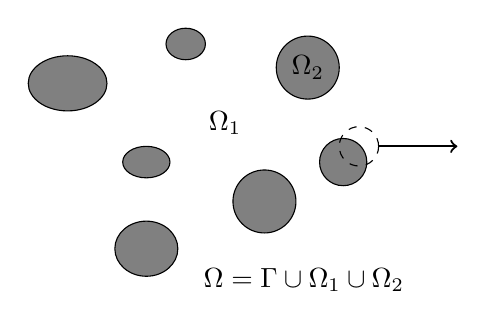
\begin{tikzpicture}
        \foreach \x/\y/\ra/\r in {
        1/3/0.2/0.25,
        2.55/2.7/0.4/0.4,
        0.5/0.4/0.35/0.4,
        2/1/0.4/0.4,
        3/1.5/0.3/0.3,
        0.5/1.5/0.2/0.3,
        -0.5/2.5/0.35/0.5}{
            \draw[fill=gray](\x,\y) ellipse(\r cm and \ra cm);
        }
        \draw[dashed](3.2,1.7)circle(0.25);
        % \draw[thick,->](3.2,1.7)++(0.1767,0.1767)--++(0.4,0.4)--++(1,0);
        \draw[thick,->](3.2,1.7)++(0.25,0)--++(1,0);
        \draw(2.55,2.7)node{$\Omega_2$};
        \draw(1.5,2)node{$\Omega_1$};
        \draw(2.5,0)node{$\Omega = \Gamma \cup \Omega_1 \cup \Omega_2$};
        % \draw(2.5,-1)node{$\Gamma = \sum_\alpha \Gamma_\alpha$};
        % \draw(2.5,-0.5)node{$\Omega_2 = \sum_\alpha \Omega_\alpha$};
    \end{tikzpicture}
    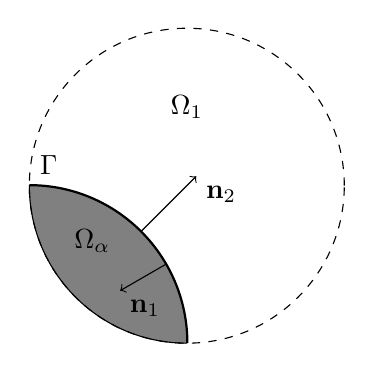
\begin{tikzpicture}%[scale = 0.9]
        \draw[very thick](0:2)arc(0:90:2)node[above right]{$\Gamma$};
        \draw[fill=gray](0:2)arc(0:90:2)arc(180:270:2);
        \draw[dashed](2,2)circle(2);
        \draw[->](1.42,1.42)--++(0.7,0.7)node[below right]{$\textbf{n}_2$};
        \draw[->](1.73,1)--++(-0.577,-0.333)node[below right]{$\textbf{n}_1$};
        \draw(2,3)node{$\Omega_1$};
        \draw(0.8,1.3)node{$\Omega_\alpha$};
    \end{tikzpicture}
    \caption{Topology of dispersed two-phase flows.}%Domain definitions and scheme of the topology of dispersed two-phase flows.}
    \label{fig:Scheme}
\end{figure}

We consider a system consisting of two phases, separated by a sharp interface $\Gamma(t)$ which evolves over time. 
For further insights into the modeling of sharp interface thermodynamics, a comprehensive review may be found in \cite{bothe2022sharp}. 
Each phase subdomain is denoted as $\Omega_1(t)$ and $\Omega_2(t)$, representing the continuous phase (1) and the dispersed phase (2) respectively (refer to Figure \ref{fig:Scheme}).
The entire domain, denoted as $\Omega$, is defined as the union of $\Omega_1$, $\Omega_2$, and $\Gamma$.
To track the position of the phase indexed $k$ and the interfaces, we introduce the phase indicator function $\chi _k$ defined as
\begin{align}
    \chi_k(\textbf{x},t) =  \left\{
      \begin{tabular}{cc}
        $1 \;\text{if} \;\textbf{x} \in \Omega_k(t)$\\
        $0 \;\text{if} \;\textbf{x} \notin \Omega_k(t)$
      \end{tabular}
      \right.
      \text{for $k = 1,2$}.
      \label{eq:PIF}
\end{align}


\subsection{Topological equations}
Using the distribution formalism, one may show that $\chi_k$ obeys the following relations \citep{drew1983mathematical,orlando2023evolution}. 
\begin{align}
    \pddt \chi_k
    + \textbf{u}_I^0 \cdot \grad \chi_k
    &= 0,
    \label{eq:dt_chi_k}\\
    \label{eq:grad_chi_k}
    \grad \chi_k
    &= - \delta_I \textbf{n}_k. 
\end{align}
where $u^0_I$ is the velocity of the interface and $\delta_I$ is the Dirac function localized on the interface.
Then, to describe the evolution of $\delta_I$ we take the gradient for \ref{eq:dt_chi_k} and the gradient of \ref{eq:grad_chi_k} which yields two equations of the interface indicator function \citep{marle1982macroscopic,morel2007surface,orlando2023evolution},
\begin{align}
    \pddt \delta_I
    + \div (\delta_I (\textbf{u}_I^0\cdot \textbf{n}) \textbf{n})
    &= \delta_I (\textbf{u}_I^0 \cdot \textbf{n})(\div\textbf{n})
    \label{eq:dt_delta_I}\\
    \grad\delta_I 
    &= \textbf{n} \cdot \grad (\textbf{n} \delta_I),
    \label{eq:grad_delta_I}
\end{align}
Notice that only the normal components of the surface velocity plays a role in this equation. 
We also employ the subscript $_I$ to indicate any quantity inherently defined on the interface such as its local velocity $\textbf{u}_I^0$. 

\ref{eq:dt_chi_k}, \ref{eq:dt_delta_I}, \ref{eq:grad_delta_I} and \ref{eq:grad_chi_k} are commonly referred to as the topological equations. 
It describes the evolution in space and time of the topology of the flow interfaces.
To enhance clarity, we will omit the time and position parameters from $\chi_k(\textbf{x},t)$ and $\delta_I(\textbf{x},t)$ in the subsequent sections.

\subsection{Local conservation equations}
\label{sec:local_eq}
Let now introduce the local conservation laws that govern the fluid inside bulk phases and the interfaces. 

\subsubsection{Inside the volumes}

Within phase $k$, we note $\rho_k$ the density, $\textbf{u}_k^0$ the local velocity and $E_k^0$ the local total energy per units of mass.
All over the domain $\Omega_k(t)$ the mass, momentum and total energy obey these conservation laws :
\begin{align}
    \label{eq:dt_rho}
    \pddt \rho_k  
    + \div (
        \rho_k\textbf{u}_k^0
    )
    &= 
    0\\
    \label{eq:dt_rhou_k}
    \pddt (\rho_k\textbf{u}_k^0)  
    + \div (
        \rho_k\textbf{u}_k^0\textbf{u}_k^0
        - \bm{\sigma}_k^0 
    )
    &= 
    \rho_k \textbf{g}\\
    \label{eq:dt_rhoE_k}
    \pddt (\rho_kE_k^0)  
    + \div (
        \rho_kE_k^0\textbf{u}_k^0
        + \textbf{q}_k^0
        - \textbf{u}_k^0 \cdot \bm{\sigma}_k^0 
        )
    &= 
    \textbf{u}_k^0 \cdot \textbf{g}  \rho_k
\end{align} 
All along this work the continuous phase will be considered as Newtonian fluid thus, $\bm{\sigma}_1^0 = - p_1^0 \bm\delta + \bm{\tau}_1^0$ where $\bm{\tau}_1^0$ is the Newtonian stress tensor with $p_1 ^0$ the local pressure and $\bm{\tau}_1^0 = \mu_1[\grad \textbf{u}_1^0+(\grad \textbf{u}_1^0)^T]$ the shear rate. 
The vector $\textbf{q}_k^0$ represent the thermal energy flux and is often model with a Fourier law : $\textbf{q}_k^0 = -\lambda \grad T_k^0$ where $T_k$ is the temperature and $\textbf{g}$ is the acceleration of gravity which will be the only body force in the present problem. 
All along this work the superscript $^0$ indicate that the variable is defied at the local or microscopic scale, in opposition to the averaged or macroscopic quantities that will be presented latter. 

The total energy is decomposed in the usual way, i.e. $E_k^0 = e_k^0 + (u_k^0)^2/2$ where  $e_k^0$ is the internal energy which represent the molecular agitation and $(u_k^0)^2/2$ is the kinetic energy per unit of mass.
This decomposition and the previous set of equations lead us to two independent equations for $e_k$ and $u_k$, namely,
\begin{align}
    \label{eq:dt_rhou_k2}
    \pddt [\rho_k(u_k^0)^2]  
    + \div [\rho_k(u_k^0)^2\textbf{u}_k^0/2 - \textbf{u}_k^0 \cdot \bm{\sigma}_k^0]
    &=
    \rho_k\textbf{u}_2^0 \cdot \textbf{g}  
    -  \bm{\sigma}_k^0 : \grad \textbf{u}_k^0,
    \\
    \label{eq:dt_rhoe_k}
    \pddt (\rho_ke_k^0)  
    + \div (
        \rho_ke_k^0\textbf{u}_k^0
        + \textbf{q}_k^0
        )
    &= 
    \bm{\sigma}_k^0 : \grad \textbf{u}_k^0. 
\end{align} 
We can observe that the viscous dissipation term, $\bm{\sigma}_k^0 : \grad \textbf{u}_k^0$,  appears with opposite sign in both of the above equations.
This indicates that $\bm{\sigma}_k^0 : \grad \textbf{u}_k^0$ is the energy that is transformed from kinetic to internal energy. 
By the use of thermodynamics equilibrium laws one can show that from the internal energy equation one can derive an equation for the local temperature \citet{ishii2010thermo}.
In this work we display the internal energy equation for completeness, no link with the temperature or any other thermodynamic quantity will be given. 
We will rather focus on the fluid and particle kinetic energy. 

\subsubsection{On interfaces}

\tb{
    dans cette section il y a une petite incoherence sur les equation energetique de surface. 
    En fait $E_I^0 = e_I^0 + (u_I^0)^2$ avec $e_I$ energie iinerne de surface qui est liée a la tension de surface par $\gamma = e_I − T_I s_I$ avec $T$ la temperature et $s$ l'entropie. bref faut que je mette tout ca au claire. 
    Pour résoudre le pbl voir\cite{ishii2010thermo}
}

On the interface $\Gamma(t)$ the conservation laws take the form of $2d$ conservation laws due to the topology of the interface. 
They are often viewed as \textit{jump condition} which make the link between the conservation equations in both phases. 
The interface mass and momentum conservation equation are well established.
However, the energy conservation law jump condition at the interface is less employed.
In the most general case the mass, momentum and energy surface equations can be written as\citep{morel2015mathematical}, 
\begin{align}
    \label{eq:dt_rhoI}
    \pddt \rho_I
    + \rho_I (\textbf{u}_I^0 \cdot \textbf{n})(\div \textbf{n})
    + \divI (\rho_I\textbf{u}_{I||}^0)
    &= 
    0
    % \Jump{
    %     \rho_k (\textbf{u}_I - \textbf{u}_k)
        % \mathbf{T}_k
    % }
    \\
    \label{eq:dt_rhoIu_I}
    \pddt (\rho_I\textbf{u}_I^0)  
    + \rho_I \textbf{u}_I^0 (\textbf{u}_I^0 \cdot \textbf{n})(\div \textbf{n})
    + \divI (
    \rho_I\textbf{u}_I^0\textbf{u}_{I||}^0
    - \bm{\sigma}_{I||}^0)
    &= 
    \rho_I \textbf{g}
    - \Jump{
        % \rho_k \textbf{u}_k (\textbf{u}_I - \textbf{u}_k)
        \bm\sigma^0_k
    }\\
    \label{eq:dt_rhoIE_I}
    \pddt (\rho_IE_I^0)  
    + \rho_IE_I^0  (\textbf{u}_I \cdot \textbf{n})(\div \textbf{n})
    + \divI (
        \rho_I E_I^0\textbf{u}_{I||}^0
        - \textbf{u}_I^0 \cdot \bm{\sigma}_I^0 
        + \textbf{q}_{I||}^0
        )
    &= 
    \textbf{u}_k^0 \cdot \textbf{g}  \rho_I
    - \Jump{\textbf{u}_k^0 \cdot \bm{\sigma}_k^0 - \textbf{q}_k^0}
\end{align} 
where, $\rho_I$ is the mass per unit of surface of the interface, $\textbf{u}_I^0$ is the local velocity of the interface $\Gamma(t)$, $\bm{\sigma}_I^0$ is the local momentum diffusive flux of surface, $\textbf{q}_I^0$ is the local internal energy diffusive flux of surface and $E_I^0 = e_I^0 + \frac{1}{2}(u_I^0)^2$ is the total energy at the interface, with $e_I^0$ the interface internal energy. 
We introduced the surface divergence operator defined as $\divI ()= (\bm\delta-\textbf{nn})\cdot \div ()$, which correspond to the divergence operator projected on $\Gamma(t)$. 
Throughout this work we use the subscript  $_{||}$ to indicate the projection of a quantity onto the plane tangential to the surface $\Gamma(t)$. 
Specifically, for an arbitrary quantity $\textbf{f}$ defined on $\Gamma(t)$, we denote its tangential projection as $\textbf{f}_{||}^0 = (\bm\delta-\textbf{nn})\cdot \textbf{f}^0$. 
Notice that the diffusive flux $\bm{\sigma}_{I||}^0$ and $\textbf{q}_{I||}^0$ appear as quantity projected on the surface tangential plane.
Indeed, it can be shown that only the tangential parts of the diffusive flux plays a role in the surface momentum balance equations, see \citet{slattery2007interfacial}.
We also introduced the notation $\Jump{\ldots}$, which is defined as $\Jump{\ldots} = \sum_{k=1}^2 [\ldots] \cdot \textbf{n}_k$.
Where $\textbf{n}_k$ is the outward normal vector associated with the domain $\Omega_k$ (see \ref{fig:Scheme}).

The formulations given by \ref{eq:dt_rho_I},\ref{eq:dt_rhoIu_I}and \ref{eq:dt_rhoI} remains quite general and needs some further simplifications. 
First we assume a thermodynamic local equilibrium everywhere at the interfaces. 
In this case the interfacial energy is closely related to the surface tension coefficient noted $\gamma$, that will be considered constant throughout this work. 
We assume that the momentum diffusive flux of surface is solely due to surface tension, therefore $\bm{\sigma}_I^0  = \gamma (\bm\delta - \textbf{nn}) = \gamma \bm\delta_{||}$ where $\gamma$ is the surface tension coefficient which will be assumed constant overall the interfaces \citep[Chapter 2]{tryggvason2011direct}.  
Note that in a more general case, interfacial viscous stress could be included into $\bm{\sigma}_{I}^0$ \citep{brenner2013interfacial,slattery2007interfacial,nadim1996concise}, nevertheless it will not be addressed in this study. 
Additionally, we assume the surface density to be negligible thus $\rho_I = 0$ and since we considered no energy accumulation at the interface $\textbf{q}_I=0$.
Also, instead of 
Consequently, the interfacial mass, momentum and total energy balance equations reduce to the common expressions :
\begin{align}
    \label{eq:dt_rho_I}
    \Jump{
        \rho_k (\textbf{u}_I - \textbf{u}_k)
        % \mathbf{T}_k
    }
    &=0, \\
    \Jump{\bm{\sigma}_k^0} 
    &=
    \divI\bm\sigma^0_{I||}
    =
    -\gamma\textbf{n}(\div \textbf{n}),
    % + \gradI\sigma 
    \label{eq:surface_tension}\\
    \label{eq:dt_rhoI_EI}
    - \Jump{\textbf{u}_k^0 \cdot \bm{\sigma}_k^0 - \textbf{q}_k^0}
    &=
    \pddt \gamma + \divI(\gamma \textbf{u}_I - \bm\sigma^0_{I||}\cdot \textbf{u}_I^0 )
    =
    + \gamma\textbf{n}\cdot \textbf{u}_{I}^0(\div \textbf{n}),
    % +
    % \label{eq:dt_rhoIe_I}
    % \Jump{ \textbf{q}_k^0}eq:dt_rho_I
    % &= 
    %  0
\end{align}
respectively. 
Where $ - \div\textbf{n}$ is twice the mean interface curvature.
% In \ref{eq:surface_tension}, we can clearly identify two contributions : the first one related to the curvature, and the second one from the non-constant surface tension coefficient along the surface. 
% The latter contribution is responsible for the Marangonie effect.
% This terms 
\ref{eq:dt_rhoI_EI} is the jump equation for the total energy.
However, in the following it will be more practical to deal with an equation for the kinetic and internal energy separately. 
Thus, we take the dot product of \ref{eq:surface_derivative}, \ref{eq:} with $\textbf{u}_I$ and subtract this new expression to \ref{eq:dt_rhoI_EI} which gives us, 
\begin{align}
    \label{eq:dt_rhoI_uI2}
    \Jump{\textbf{u}_k^0 \cdot \bm{\sigma}_k^0}
    &=
    -\gamma\textbf{n}\cdot \textbf{u}_{I}^0(\div \textbf{n})\\
    \label{eq:dt_rhoIe_I}
    \Jump{ \textbf{q}_k^0}
    &= 
     0
\end{align}
for the interface kinetic energy and the internal interface energy, respectively. 
Notice that this decomposition is possible only under the assumption of no mass transfer in which case $\textbf{u}_I^0=\textbf{u}_k^0$ for $k =1,2$ and a constant surface tension coefficient.


In the perspective of ensemble averaging the objective of the next two subsections is to extend the domain of definition of these two equations to the whole space $\Omega$.


\subsubsection{Generic formulation}

For ease of understanding, we now introduce generic conservation laws in the volumes and on the interfaces. 
Let $f_k^0(\textbf{x},t)$ denote a volumetric quantity of arbitrary tensorial order defined in $\Omega_k(t)$.
Likewise, let $f_I^0(\textbf{x}_I,I)$ represent an arbitrary surface property defined on $\Gamma(t)$.
Using the strategy outlined in \citep{bothe2022sharp,morel2015mathematical,slattery2007interfacial}, we can derive the local conservation equations for both $f_k^0(\textbf{x},t)$ and $f_I^0(\textbf{x}_I,t)$, that is,  
\begin{align}
    \label{eq:dt_f_k}
    \pddt f_k^0
    +\div \left(
        f_k^0\textbf{u}_k^0
        - \mathbf{\Phi}_k^0
        \right)
    &= 
    s_k^0
    & \text{ in } \Omega_k(t),&\\
    \pddt f_I^0 
    + f_I^0 (\textbf{u}_I \cdot \textbf{n})(\div \textbf{n})
    +\divI
    (f_I^0 \textbf{u}_{I||}^0
        - \mathbf{\Phi}_{I||}^0 )
    &= 
    s_I^0
    - \Jump{
       f_k (\textbf{u}_I^0 - \textbf{u}_k^0)
       + \mathbf{\Phi}_k^0
    } 
    & \text{ on } \Gamma(t),&
    \label{eq:dt_f_I}
\end{align}
respectively.
The tensors $\mathbf{\Phi}_k^0(f_k)$ and $\mathbf{\Phi}_{I||}^0(f_I)$ represent the non-convective fluxes corresponding to $f_k^0$ and $f_I^0$. 
Notice that $\mathbf{\Phi}_{I||}^0$ also carries the $_{||}$ subscript which implies that only the tangential component of this tensor remain in the surface balance equation. 
Similarly, $s_k^0(f_k^0)$ and $s_I^0(f_I^0)$ represent the source terms of $f_k^0$ and $f_I^0$, respectively.
Notice, that in \ref{eq:dt_f_I} we kept the mass transfer term $f_k (\textbf{u}_I^0 - \textbf{u}_k^0)$ for purpose of generality. 
For practical uses, note that the advecting term in \ref{eq:dt_f_I}can be written in the more compact form $f_I^0 (\textbf{u}_I \cdot \textbf{n})(\div \textbf{n})
+\divI(f_I^0 \textbf{u}_{I||}^0) = \divI(f_I^0 \textbf{u}_I^0)$ by noticing that $\textbf{n}\cdot\gradI(\ldots) = 0$ and $\divI\textbf{n} = \div\textbf{n}$ \citep{nadim1996concise}.
It is important to note that \ref{eq:dt_f_k} and \ref{eq:dt_f_I} are solely defined within $\Omega_k(t)$ and $\Gamma(t)$, respectively.
This was also the case for the equations presented in the last two subsections. 
Consequently, these equations are referred to as local conservation equations. 


\subsection{The two-fluid formulation}
The presence function $\chi_k$, and the Dirac delta function $\delta_I$, allow the extension of local conservation equations to the entire flow domain $\Omega$. 
This extension is achieved by employing the methodology introduced by \citet{drew1983mathematical} and \citet{kataoka1986local} for the conseriving laws inside the volume (\ref{eq:dt_f_k}).
For any local quantities $f_k^0$ defined in $\Omega_k(t)$, we assign the field $\chi_k f_k^0$, which is defined over the entire domain $\Omega$. The two-fluid formulation may be obtained by multiplying \ref{eq:dt_f_k} by $\chi_k$. 
Using \ref{eq:dt_chi_k} and \ref{eq:grad_chi_k} we obtain
\begin{equation}
    \pddt (\chi_k f_k^0)
    + \div (
        \chi_k f_k^0 \textbf{u}_k^0
        - \chi_k \mathbf{\Phi}_k^0 
        )
    = 
    \chi_k s_k^0
    + \delta_I\left[
        f_k^0
        \left(
            \textbf{u}_I^0
            - \textbf{u}_k^0
        \right)
        + \mathbf{\Phi}_k^0
    \right]
    \cdot \textbf{n}_k.
    \label{eq:dt_chi_k_f_k}
\end{equation}
Likewise, for any surface property $f_I^0$ defined on $\Gamma(t)$, we assign the field $\delta_I f_I^0$, which is also defined all over $\Omega$. 
Following the approach outlined \citet[Appendix 2]{marle1982macroscopic} we can generalize \ref{eq:dt_f_I} to the 3D space. 
Making use of the topological equations \ref{eq:dt_delta_I} and \ref{eq:grad_delta_I} gives,
\begin{equation}
    \pddt (\delta_If_I^0)  
    + \div (
        \delta_I f_I^0 \textbf{u}_I^0
        - \delta_I \mathbf{\Phi}_{I||}^0 
        )
    = 
    \delta_Is_I^0
    - \delta_I\Jump{
    f_k^0 (\textbf{u}_I^0 - \textbf{u}_k^0)
    + \mathbf{\Phi}_k^0} 
    \label{eq:dt_delta_I_f_I}
\end{equation}
which correspond to the conservation equation for $\delta_If_I^0$.
The last term on the right hands side of \ref{eq:dt_chi_k_f_k} represent the phase transfer of $f_k$ across the interfaces and the non-convective fluxes across phases.
The set of equations formed by \ref{eq:dt_chi_k_f_k} for $k =1,2$ is commonly known as the \textit{two-fluid} formulation of multiphase flows, to which we add the \textit{jump condition} across the phase given by \ref{eq:dt_delta_I_f_I} \citep{morel2015mathematical,tryggvason2011direct,drew1983mathematical,kataoka1986local}. 

\tb{this formulation is useful for the bulk stress}
In this work, we prefer to think of those equations as a set of three equations formed by \ref{eq:dt_chi_k_f_k} for $k=1,2$ and \ref{eq:dt_delta_I_f_I}. 
We define the \textit{bulk} property $\textbf{f}$ as $\textbf{f}^0 = \sum_k \chi_k \textbf{f}_k^0 + \delta_I \textbf{f}_I^0$ where $\textbf{f}^0$ represents any property of the flow of arbitrary tensorial order at the local scale.
Then by summing \ref{eq:dt_chi_k_f_k} for $k=1,2$ and \ref{eq:dt_delta_I_f_I}, one obtain the \textit{single-fluid} formulation conservation equation, namely,
\begin{equation}
   \pddt f^0
   + \div (
       f^0 \textbf{u}^0
       -  \mathbf{\Phi}^0 
    )
   = s^0. 
   \label{eq:dt_f}
\end{equation}
It should be noted that in the literature we rather define the \textit{bulk} quantities as $f^0 = \sum_k \chi_k f_k^0$, while the interfacial component is treated as a source term in \ref{eq:dt_f} \citep{morel2015mathematical,tryggvason2011direct,drew1983mathematical}. 
Nevertheless, we want to point out here that with this definition we recover a classic transport equation for the bulk quantity $f^0$ which makes the whole system of equation consistent.




\subsection{The averaged conservation equations}
In this study, we employ the ensemble average technique to establish the averaged conservation equations. 
This method is just one of several averaging approaches, including the volume average method \citep{jackson1997locally} and time averaging \citep{ishii2010thermo}. 
Despite their differences, all these techniques yield the same set of averaged equations \citep{jackson1997locally,zhang1997momentum}.
In the following we recall some properties of the ensemble average operator. 
Let, $P(\FF)$ be the probability density function that describe the probability of finding the flow in the configuration $\FF$. 
It follows from this definition, that the ensemble average of an arbitrary local property $f^0(\textbf{x},t;\FF)$ defined on the whole space $\Omega$, is,
\begin{equation}
    f(\textbf{x},t)
    = \avg{f^0}(\textbf{x},t)
    =\int f^0(\textbf{x},t;\FF) d\mathscr{P}. 
    \label{eq:avg}
\end{equation}  
Note that we dropped the super script $^0$ on $f$ to indicate that this is an averaged quantity. 
Therefore, all variables denoted with a $^0$ are functions of $(\textbf{x}, t; \FF)$, whereas all macroscopic variables are averaged over all $\FF$ and thus depend only on $(\textbf{x}, t)$.
The ensemble average quantities are assumed to satisfy the following properties \citep{drew1983mathematical}
\begin{align}
    \avg{f^0+h^0} &= f+h, \\ 
    \avg{\avg{f^0}h^0} &= fh, \\
    \avg{\pddt f^0} 
    &= \pddt f, \\ 
    \avg{\grad f^0}
    &= \grad f. 
    \label{eq:avg_properties}
\end{align}
were $f$ and $h$ are two arbitrary Eulerian fields. The first two relations are called the Reynolds' rules, the third one is the Leibniz' rule and the last one, the Gauss' rule \citep{drew1983mathematical}.
Additionally, for any phase quantity defined in $\Omega_k$ we introduce the definition, 
\begin{equation}
    \phi_k f_k (\textbf{x},t) = \avg{\chi_k f_k^0}
    \label{eq:1_avg}
\end{equation}
where, $\phi_k(\textbf{x},t) = \avg{\chi_k}$ is the volume fraction of the phase $k$
and $f_k(\textbf{x},t)$ the average of the field $f_k^0$ conditioned on the presence of the phase $k$ at $\textbf{x}$ and time $t$.
Equally, for interface quantities we have 
\begin{equation}
    \phi_I f_I (\textbf{x},t) = \avg{\delta_I f_I^0}
\end{equation}
with $\phi_I = \avg{\delta_I}$ the interfacial area concentration function and $f_I(\textbf{x},t)$ the average of $f^0_I(\textbf{x},t,\FF)$ conditioned on the presence of an interface at $\textbf{x}$ and time $t$. 
The fluctuation of a phase-averaged quantity around its mean is defined by,
\begin{align}
    f_k' = f_k^0 - f_k.
    && f_I' = f_I^0 - f_I.
    \label{eq:def_fluctu}
\end{align}
Thus, the product $\avg{\chi_k f^0_kg^0_k}$ can be decomposed as $\avg{\chi_k f_k^0g_k^0}=\phi_k f_kg_k + \avg{\chi_k f'_kg'_k}$. 


Applying the ensemble average on \ref{eq:dt_chi_k_f_k} and \ref{eq:dt_delta_I_f_I} and considering the properties from \ref{eq:avg_properties} together with \ref{eq:def_fluctu} yields the general form of the averaged equations of multiphase flows, namely,
\begin{align}
    \pddt (\phi_k f_k)
    +\div (\phi_k f_k \textbf{u}_k - \mathbf{\Phi}_k^\text{eq})
    &= 
    \phi_k s_k
    + \avg{\delta_I\left[
        \mathbf{\Phi}_k^0
        + f_k^0
        \left(
            \textbf{u}_I^0
            - \textbf{u}_k^0
        \right)
    \right]
    \cdot \textbf{n}_k} ,
    \label{eq:avg_dt_chi_f}\\
    \pddt (\phi_I f_I)
    +\div (\phi_I f_I \textbf{u}_I- \mathbf{\Phi}_{I}^\text{eq})
    &= 
    \phi_I s_I
    - \avg{\delta_I 
    \Jump{
    f_k^0 (\textbf{u}_I^0 - \textbf{u}_k^0)
    + \mathbf{\Phi}_k^0
    } 
     }.
    \label{eq:avg_dt_delta_f}
\end{align}
where $\mathbf{\Phi}_{I}^\text{eq}$ and $\mathbf{\Phi}_{I}^\text{eq}$ are the equivalent non-convective fluxes defined as 
\begin{align*}
    \mathbf{\Phi}_k^\text{eq}
    = \avg{\chi_k f_k' \textbf{u}_k'}
    - \phi_k \bm\Phi_k,
    &&
    \mathbf{\Phi}_{I}^\text{eq}
    = \avg{\delta_I f_I' \textbf{u}_I'}
    - \phi_I \bm\Phi_I. 
\end{align*}
% Note that while all terms are just the average of their local counterpart, the covariance term $\avg{\chi_k f_k' \textbf{u}_k'}$ and $\avg{\delta_I f_I' \textbf{u}_I'}$ arise fropurely mathematical 
These equations are to be solved for the averaged field $\phi_k,\phi_I,f_k$ and $f_I$ with a complementary equation of volume conservation, i.e. $\phi_1+\phi_2+\phi_I w_I = 1$ where $w_I$ is the mean width of the interfaces.
% Thus, all term in these equations must be expressed as a function of $\phi_k,\phi_I,f_k$ and $f_I$. 
The main differences between these equations and their microscale counterparts (\ref{eq:dt_f_k} and \ref{eq:dt_f_I}) are:
(1) The unknowns are averaged quantities,
(2) Factors $\phi_k$ and $\phi_I$ are introduced in front of all the terms, and
(3) The additional stresses $\avg{\chi_k f_k' \textbf{u}_k'}$ and $\avg{\delta_I f_I' \textbf{u}_I'}$ appear, representing the covariance between the conserved quantity and the local velocities.  
For a complete understanding, we derived the mass, momentum, and energy averaged equations in \ref{ap:two-fluid_model}. 
Especially we demonstrate how to derive the secondary equations of the averaged energy $E_k$, i.e. the equation for the mean internal energy $e_k$, the pseudo turbulent energy (defined therein) and the averaged kinetic energy $(u_k)^2/2$.  

It is important to highlight that the two-fluid model fails to adequately distinguish between the two phases, as evidenced by the \textit{symmetry} $k = 1$ and $2$ in the aforementioned equations. This symmetry does not hold physically because the dispersed phase possesses a distinct topological nature compared to the continuous phase. 
More importantly, in a dispersed two phase flow system the closure terms are expressed as a function of the Lagrangian properties of the particles whereas this system of equation provides us with continuously averaged quantities. 
Specifically, the mean drag force term in the averaged momentum equation is expressed as a function of the  center of mass velocity of the particles. 
Whereas this system of equation provides us with the phase averaged velocity of the whole phase not with no consideration for the center of mass.  
Therefore, in the subsequent section, we will introduce a kinetic model specifically devoted to the dispersed phase. 
As illustrated below, the equations governing the dispersed phase are more comprehensive as they bear a resemblance to the equations governing a single particle.



\section{Lagrangian equations for the dispersed phase}
\label{sec:Lagrangian}

While \ref{eq:dt_chi_k_f_k} and \ref{eq:dt_delta_I_f_I} describe multiphase-flow in a general manner, they do not leverage the topology of the dispersed phase. 
Therefore, in this section, we present a Lagrangian-based model capable of describing the dispersed phase with an arbitrary order of accuracy.

\subsection{Fundamental properties}

At this stage, it is crucial to define some fundamental properties associated to each particle.
Following the strategy of \citet{lhuillier2009rheology,lhuillier1992volume,zaepffel2011modelisation} and \citet[Chapter 2]{morel2015mathematical}
we define the mass, position of center of mass, momentum and total energy of the particle $\alpha$, such as,
\begin{align}
    &m_\alpha(t)
    = \int_{\Omega_\alpha(t)} \rho_2  d\Omega,
    % &&
    &\textbf{x}_\alpha(t)
    = \frac{1}{m_\alpha(t) }\int_{\Omega_\alpha(t)} \rho_2 \textbf{x} d\Omega,\\
    % &&
    &\textbf{p}_\alpha(t) 
    = \int_{\Omega_\alpha(t)} \rho_2 \textbf{u}_2^0 d\Omega,
    % &&
    & m_\alpha E_\alpha(t) 
    = \int_{\Omega_\alpha(t)} \rho_2 [e_2^0 + (u_2^0)^2/2] d\Omega,
    \label{eq:position_and_momentum_def}
\end{align}
respectively. 
Where $\Omega_\alpha$ is the domain occupied by the particle $\alpha$ (see \ref{fig:Scheme}). 
Subsequently, we define the velocity of the particle's center of mass, denoted as $\textbf{u}_\alpha$ which is given by $\textbf{u}_\alpha = \ddt \textbf{x}_\alpha$. 
The derivation of $\ddt \textbf{x}_\alpha$ is straightforward but requires some algebra which are detailed in \ref{ap:velocity_definition}. 
The final expression reads,
\begin{equation}
    \textbf{u}_\alpha(t) = \frac{1}{m_\alpha(t)} \left(
        \textbf{p}_\alpha(t)
        +  \int_{\Sigma_\alpha(t)} \rho_2 \textbf{r} (\textbf{u}_I^0 - \textbf{u}_2^0)\cdot \textbf{n}_2 d\Sigma
        \right),
        \label{eq:dt_y_alpha}
\end{equation}
where $\textbf{r}(\textbf{x},t) = \textbf{x} - \textbf{x}_\alpha(t)$. 
In Equation \ref{eq:dt_y_alpha}, it can be observed that the first component of the velocity represents the linear momentum divided by the mass of the particle. 
This corresponds to the mass-averaged velocity over the volume of the particle.
The second term in Equation \ref{eq:dt_y_alpha} arises from the contribution of anisotropic mass transfer across the surface of the particle. 
This mass transfer leads to the motion of the particle's center of mass, thereby contributing to the total velocity.
To illustrate this concept, let us consider a fixed drop with no momentum lying over a very hot plate.
In this scenario, we assume that the plate is sufficiently hot to induce evaporation, specifically on the bottom portion of the drop.
Hence, under the effect of an anisotropic evaporation flux one may expect the second term to be non-negligible.
Consequently, the center of mass of the drop has a non-zero velocity in the opposite direction of the plate, even though the momentum is assumed to be zero.
We can also consider the case of the nucleation of a bubble in water. 
In this case, although the particle momentum is null at all time the center of mass of the particle moves due to the growth of the particle. 
In both cases, we need to take into account the mass transfer term in \ref{eq:dt_y_alpha}, while the first term is negligible. 
Note that \ref{eq:dt_y_alpha} generalized usual expression of the center of mass velocity whom neglect the second term.
In the following, we discard the time dependency notation for all Lagrangian quantities denoted by the subscript $_\alpha$ and also $\Sigma(t)$ and $\Omega_\alpha$.
Nevertheless, the reader must understand that all Lagrangian quantities and integration domains subscribed by $_\alpha$ are time dependent. 

The particle's internal relative motions or the \textit{inner velocity} is given by $\textbf{w}_2^0(\textbf{x},t) = \textbf{u}_2^0(\textbf{x}) - \textbf{u}_\alpha(t)$.
Thus, from its definition in \ref{eq:position_and_momentum_def}, we can rewrite the momentum as follows,
\begin{equation}
    \label{eq:momentum_definition_1}
    \textbf{p}_\alpha
    = m_\alpha \textbf{u}_\alpha
    + \int_{\Omega_\alpha} \rho_2 \textbf{w}_2^0 d\Omega.
\end{equation}
Alternatively, by manipulating \ref{eq:dt_y_alpha}, we obtain,
\begin{equation}
    \textbf{p}_\alpha
    =  m_\alpha \textbf{u}_\alpha
    - \int_{\Sigma_\alpha} \rho_2\textbf{r}(\textbf{u}_I^0 - \textbf{u}_2^0)\cdot \textbf{n}_2 d\Sigma
    \label{eq:momentum_definition}
\end{equation}
Therefore, the momentum of a particle can be seen as a sum of the mean velocity plus the integral of the fluctuation (\ref{eq:momentum_definition_1}), with the latter being equivalent to minus the first moment of mass transfer term (\ref{eq:momentum_definition}).
Indeed, by identification we obtain : $\int_{\Omega_\alpha} \rho_2 \textbf{w}_2^0 d\Omega =\int_{\Sigma_\alpha}  \rho_2\textbf{r} (\textbf{u}_I^0 - \textbf{u}_2^0)\cdot \textbf{n}_2 d\Sigma$. 
The essential aspect of this relation highlighted here is that the internal velocity fluctuations within a fluid particle do not contribute to the total linear momentum $\textbf{p}_\alpha$, as long as the anisotropic mass transfer is negligible.  
Additionally, the total energy $E_\alpha$ can be decomposed following a similar procedure which leads us to, 
\begin{equation*}
    \label{eq:E_alpha_def}
    m_\alpha E_\alpha(t) 
    = m_\alpha e_\alpha 
    + W_\alpha
    + m_\alpha (u_\alpha)^2/2
    % + \textbf{u}_\alpha \cdot \int_{\Omega_\alpha(t)} \rho_2  \textbf{w}_2^0 d\Omega
\end{equation*}
where we introduced the internal kinetic energy : $W_\alpha = \int_{\Omega_\alpha(t)} \rho_2  (w_2^0)^2/2 d\Omega$. 
In that expression mass transfer have been neglected. 
Anyhow, the total energy of a particle is the sum of its internal energy $e_\alpha$, internal kinetic energy $W_\alpha$ and the kinetic energy  due to its own center of mass displacement $u_\alpha^2/2$. 
To gain in understanding, let's express $W_\alpha$ in the case of a solid particle.
The velocity inside a solid particle can be expressed : $\textbf{u}_2^0(\textbf{x}_\alpha + \textbf{r}) = \textbf{u}_\alpha + \textbf{r}\times \bm{\omega}_\alpha$ where $\bm{\omega}_\alpha$ is the angular velocity.  
In this case, $W_\alpha = \bm{\omega}_\alpha\bm{\omega}_\alpha\cdot \mathcal{I}_\alpha$ where $\mathcal{I}_\alpha$ is the inertia matrices of the particle. 
As a matter of facts for solid particles $W_\alpha$ represents the angular kinetic energy for solid particles.
Thus, for particles with fluid internal motion, $W_\alpha$ is just a more general definition of the particle internal kinetic energy. 

\subsection{Conservation laws}
We assign to a particle indexed, $\alpha$, occupying the domain $\Omega_\alpha$ (see \ref{fig:Scheme}) an arbitrary Lagrangian property $q_\alpha$ defined by $q_\alpha  = \int_{\Omega_\alpha} f_2^0(\textbf{x},t) d\Omega$.
Similarly, we define $q_{I\alpha} = \int_{\Sigma_\alpha} f_I^0(\textbf{x},t) d\Sigma$ as being an integrated surface property associated to the particle $\alpha$.


To describe the evolution of any arbitrary Lagrangian quantity $q_\alpha$, we need to establish its time derivative.
Since, $q_\alpha$ is an integral quantity with a time-dependent domain of integration, we apply the general Reynolds transport theorem for volume integral (exposed in \ref{ap:math}) to compute its time derivative \citep{morel2015mathematical}.
This yields the following expression :
\begin{equation}
    \ddt  q_\alpha
    = \int_{\Omega_\alpha}\left[ \pddt f_2^0 + \div\left(f_2^0\textbf{u}_2^0\right) \right]d\Omega\\
    + \int_{\Sigma_\alpha} f_2^0 (\textbf{u}_I^0-\textbf{u}_2^0)\cdot \textbf{n}_2 d\Sigma.
\end{equation}
By substituting the integrand of the first integral on the right-hand side (RHS) with \ref{eq:dt_f_k} we obtain the conservation laws of the quantity $q_\alpha$, namely,  
\begin{equation}
    \ddt  q_\alpha
    = \int_{\Omega_\alpha} s_2^0 d\Omega
    + \int_{\Sigma_\alpha} \left[
        f_2^0 (\textbf{u}_I^0-\textbf{u}_2^0) 
        + \mathbf{\Phi}_2^0 
        \right] \cdot \textbf{n}_2 d\Sigma,
    \label{eq:dt_q_alpha}
\end{equation}
The first term on the RHS accounts for the total contribution of the source term $s_2^0$ to the particle $\alpha$.
While, The second term on the RHS is the surface integration of the exchange terms, which includes the phase transfer flux $f_2^0 (\textbf{u}_I^0-\textbf{u}_2^0)$ and the diffusive flux $\mathbf{\Phi}_2^0$. 
For clarity, let us consider the specific case of the momentum balance, i.e. when $q_\alpha = \textbf{p}_\alpha$.
In this situation, the first term reads as $\int_{\Omega_\alpha} \rho_2\textbf{g} d\Omega$ and represents the total weight acting on the particle $\alpha$. 
Likewise, the second term represents the total source of momentum due to phase transfer, and it is expressed as, $\int_{\Sigma_\alpha} \rho_2 \textbf{u}_2^0 (\textbf{u}_I^0-\textbf{u}_2^0)\cdot\textbf{n}_2 d\Sigma$. 
Lastly, $\int_{\Sigma_\alpha} \bm{\sigma}_2^0\cdot\textbf{n}_2 d\Sigma$ represents the resultant of the hydrodynamic forces acting on the surface of the particle.
It is important to notice that under this form, the exchange terms are expressed as integrals of dispersed phase fields denoted by the subscript $_2$.
Nevertheless, depending on the nature of the dispersed phase, these fields may not always be defined.
For infinitely rigid particles it is indeed the case since, the stress $\bm{\sigma}_2^0$ isn't defined.  
Hence, our objective is to express these exchange terms, in terms of the continuous phase field quantities instead of the dispersed phase field, i.e. in terms of $\mathbf{\Phi}_1^0$ and $\textbf{u}_1^0$ rather than $\mathbf{\Phi}_2^0$ and $\textbf{u}_2^0$. 

To address this issue, let us derive the conservation equation for the integrated surface property $q_{I\alpha}$.
To differentiate time-varying surface integrals within time, we can use the general Leibniz rule (see \ref{eq:Leibnitz}), to derive the following expression :
\begin{equation}
    \ddt  q_{I\alpha}
    = \int_{\Sigma_\alpha} \left[
        \pddt f_I^0
        +   \gradI \cdot (\textbf{u}_I^0f_I^0)
    \right]d\Sigma.
    \label{eq:surface_derivative}
\end{equation}
Substituting the RHS terms of \ref{eq:surface_derivative} using \ref{eq:dt_f_I}, and making use of the surface divergence theorem on closed surfaces (see \ref{eq:surf_div_theorem}), gives,
\begin{equation}
    \ddt  q_{I\alpha}
    = \int_{\Sigma_\alpha} 
        s_I^0
    d\Sigma
    - \int_{\Sigma_\alpha} \Jump{
        f_k^0 (\textbf{u}_I^0 - \textbf{u}_k^0)
        + \mathbf{\Phi}_k^0
    }
    d\Sigma.
    \label{eq:dt_q_I_alpha}
\end{equation}
This equation can be interpreted as the surface conservation equation for the integrated surface property $f_I$, or as the flux jump condition integrated on a closed surface. 
Notice that $\bm{\Phi}_{I}^0$ isn't present in this balance equation. 
This is due to the fact that as mentioned earlier, only the tangential components of $\bm{\Phi}_{I}^0$ appear inside the surface balance equation, while we perform an integration over a closed surface which is null due to \ref{eq:surf_div_theorem}. 

As discussed above we wish to get rid of $\mathbf{\Phi}_2^0$ in \ref{eq:dt_q_alpha}. To achieve this, we treat the particle's volume and surface as a unified entity and derive a conservation equation for $q_\alpha^\text{tot} = q_\alpha + q_{I\alpha}$. 
This is done by summing \ref{eq:dt_q_alpha} and \ref{eq:dt_q_I_alpha} which leads to, 
\begin{equation}
    \ddt  q_\alpha^\text{tot}
    = 
    \int_{\Omega_\alpha} s_2^0 d\Omega
    + \int_{\Sigma_\alpha} s_I^0 d\Sigma
    + \int_{\Sigma_\alpha} \left[
        f_1^0 (\textbf{u}_I^0-\textbf{u}_1^0) 
        + \mathbf{\Phi}_1^0 
        \right] \cdot \textbf{n}_2 d\Sigma. 
    \label{eq:dt_q_alpha_tot}
\end{equation}
This equation is the general form of the linear conservation law of $\chi_2 f_2^0 + \delta_I f_I^0$ for the system consisting of the particle volume $\Omega_\alpha$, and its surface $\Sigma_\alpha$. It is applicable to any particle immersed into a continuous phase following the local conservation,\ref{eq:dt_f_k} and \ref{eq:dt_f_I}.
We refer to this equation as the zeroth-order conservation equation or the linear conservation law for the particle $\alpha$.

Following the same assumption as in \ref{sec:local_eq}, i.e. we consider no mass transfer and weightless interfaces, the Lagrangian  mass, momentum and energy equations for a single particle can be derived using the generic form \ref{eq:dt_q_alpha_tot} and reads as, 
\begin{align}
    \label{eq:dt_m_alpha}
    \ddt m_\alpha
    &= 
    0\\
    \label{eq:dt_p_alpha}
    \ddt (m_\alpha \textbf{u}_\alpha)
    &= 
    m_\alpha\textbf{g}
    +  \intS{\bm{\sigma}_2^0 \cdot \textbf{n}_2}\\
    \label{eq:dt_E_alpha}
    \ddt (m_\alpha E_\alpha + s_\alpha \gamma)
    &= 
    m_\alpha \textbf{u}_\alpha \cdot \textbf{g}
    +\textbf{u}_\alpha \cdot \intS{\bm{\sigma}_2^0 \cdot \textbf{n}_2}   
    +\intS{\textbf{w}_1^0 \cdot \bm{\sigma}_1^0 \cdot  \textbf{n}_2} 
    - \intS{\textbf{q}_2^0 \cdot \textbf{n}_2}
\end{align}
where  $\int_{\Sigma_\alpha}  \bm{\sigma}_1^0 \cdot \textbf{n}_2 d\Sigma$ is the resultants of the hydrodynamic force and $\int_{\Sigma_\alpha} \textbf{q}_1^0 \cdot \textbf{n}_2 d\Sigma$ is the resultants of the surface heat flux. 
The second term on the right hands side of the energy equation is the work produced by the mean force and the translational motion of the droplets, while $\intS{\textbf{w}_1^0 \cdot \bm{\sigma}_1^0 \cdot  \textbf{n}_2}$ is the work produced by the local forces and local motion of the fluid at the surface of the particle.
Since we integrated the energy over the particle's volume and its surface, we explicitly made appear the surface energy $\gamma s_\alpha$ within the derivative operator. 
Note that these equations does not explicitly account for inter-particle interactions. 
However, it is possible to include manually such forces by noticing that the surface external stress flux $\bm{\sigma}_1^0$ is the sum of hydrodynamic and particles-particles interaction forces, regardless it is pure contact forces from direct contact or a force mediated through the carrier fluid.
From this consideration it is possible to split every term involving the stress $\bm{\sigma}_1^0$ into two terms representing these contributions. 
Same comments can be made for the heat flux $\textbf{q}_1^0$. 
Although this distinction is important, for purpose of clearly we will stay general, and we will keep the fluxes $\bm{\sigma}_1^0$ and $\textbf{q}_1^0$ as such. 

In the spirit of the energy decomposition exposed in \ref{eq:E_alpha_def} the total energy equation can be split into three equations, one for the center of mass kinetic energy, internal motion and internal kinetic energy, namely,  
\begin{align}
    \label{eq:dt_u2_alpha}
    \frac{1}{2}\ddt (m_\alpha u_\alpha^2)
    &= 
    \textbf{u}_\alpha\cdot
    \textbf{g}m_\alpha
    + 
    \textbf{u}_\alpha\cdot
    \textbf{f}_\alpha,\\
    \label{eq:dt_w2_alpha}
    \ddt W_\alpha 
    &= 
    \intS {\textbf{w}_1^0 \cdot \bm{\sigma}_1^0 \cdot \textbf{n}_2 }
    - \intO{ \bm{\sigma}_2^0 : \grad\textbf{u}_2^0 }
    - \ddt (s_\alpha \gamma) 
    \\
     \label{eq:dt_e_alpha}
    \ddt (m_\alpha e_\alpha )
    &= 
     \intO{ \bm{\sigma}_2^0 : \grad\textbf{u}_2^0  }
    -  \intS{\textbf{q}_1^0\cdot \textbf{n}_2 } 
\end{align}
respectively. 
Note that in \citet{eq:dt_w2_alpha} the use of \ref{eq:dt_rhoI_uI2} makes appear explicitly the derivative of the surface energy $s_\alpha \gamma$. 
Note that under this form we see that the energy loss in the deformation represented by $W_p$ will be gathered in the surface energy which will in turn act as a source term in the internal kinetic energy motion.
The surface tension plays the role as a spring in the energy balance.   
From this set of equation we can easily see that the rate of dissipation terms $\intS{\bm{\sigma}_2^0 : \grad\textbf{u}_2^0}$ represent an energy sink in the equation of $W_\alpha$ while it is a source term in the internal energy equation. 
As it has been observed in the previous section, this terms convert the energy of internal motion to molecular agitation. 
However, the interplay between the center of mass  kinetic energy and the internal fluctuation is not obvious and has no common term with the heat and internal kinetic energy equation.
In fact, we will see that the transfer between these scales is archived thought the fluid phase pseudo turbulent energy. 


Finally, we would like to highlight that  due to the consideration of closed surface, the diffusive flux $\mathbf{\Phi}_I$, plays no role at all in \ref{eq:dt_q_alpha_tot}.
Therefore, in the case of the linear momentum conservation law, the contribution of the surface tension forces exposed in \ref{eq:surface_tension}, do not contribute to the momentum balance in \ref{eq:dt_p_alpha}.
As a consequence, even in the presence of local Marangoni forces, the resultant of the local surface tension forces cancels out in the linear momentum balance.
This fact has already been demonstrated by \citet{hesla1993note} who showed that the surface tension force does not contribute to the linear and angular momentum balance. 
Here, we have provided the general proof that the interfacial diffusive flux $\mathbf{\Phi}_I^0$, which is present at the local scale according to \ref{eq:dt_f_I}, does not contribute to the zeroth-order conservation law of a particle with a closed surface.
This is therefore applicable to other conservation equations, such as the surface energy balance or the surface mass balance of constituents, where surface diffusive fluxes are also present \citep{bothe2022sharp,manikantan2020surfactant}. 

Nevertheless, it is known that surface tension forces impact the hydrodynamic of droplets and bubbles \citep{kentheswaran2022direct,pesci2018computational}. 
Therefore, if the diffusive flux of surface are not involved in the linear conservation law, it must appear at some point in the momentum description of Lagrangian particles. 
To find out where this contribution arise we shall describe the particle with a higher level of accuracy. 
This is the purpose of the next section. 

\subsection{First order moment equations}

To better describe the local properties within the particles, we now introduce the first moment or the dipole of a particle.
We define the first moment of any properties $f_2^0$ and $f_I^0$ by respectively,
\begin{align}
    &\mathcal{Q}_\alpha 
    = \int_{\Omega_\alpha} \textbf{r} f_2^0 d\Omega,
    &\text{and}&
    &\mathcal{Q}_{I\alpha}
    = \int_{\Sigma_\alpha} \textbf{r} f_I^0 d\Sigma,
    \label{eq:first_moment_definition}
\end{align}
where we recall that $\textbf{r} = \textbf{x} - \textbf{x}_\alpha$ is the distance between any point inside $\Omega_\alpha$ or $\Sigma_\alpha$, to the center of mass of the particle $\alpha$.
It is then possible to differentiate these moments with respect to time in order to obtain their conservation laws.
Indeed, considering \ref{eq:dt_f_k}, \ref{eq:dt_f_I} and applying the Leibniz rule for volume and surface integrals (see \ref{eq:Reynolds} and \ref{eq:Leibnitz} respectively), we can show equally that,
\begin{align}
    \ddt \mathcal{Q}_\alpha
    &= \int_{\Omega_\alpha} \left(
        \textbf{r} s_2^0         
        + f_2^0  \textbf{w}_2^0 
        - \mathbf{\Phi}_2^0
    \right) d\Omega,
    + \int_{\Sigma_\alpha} \textbf{r} \left[
        \mathbf{\Phi}_2^0
        + f_2^0 (\textbf{u}_I^0-\textbf{u}_2^0)
    \right]\cdot \textbf{n}_2  d\Sigma 
    \label{eq:dt_Q_alpha}\\
    \ddt \mathcal{Q}_{I\alpha}
    &= \int_{\Sigma_\alpha} \left(
        \textbf{r}s_I^0
        + f_I^0 \textbf{w}_I^0
        - \mathbf{\Phi}_{I||}^0
    \right) d\Sigma,
    - \int_{\Sigma_\alpha}\textbf{r} 
    \Jump{\mathbf{\Phi}_k^0
        + f_k^0 (\textbf{u}_I^0 - \textbf{u}_k^0)
    }
    d\Sigma
    \label{eq:dt_Q_I_alpha}
\end{align}
where $\textbf{w}_I^0 = \textbf{u}_I^0 - \textbf{u}_\alpha$.
The detailed derivation of \ref{eq:dt_Q_alpha} is provided in \ref{ap:moment_derivative}.
The derivation of \ref{eq:dt_Q_I_alpha} follows a similar procedure. 
% \JL{je n'ai pas relu la derivation detaillee en annexe, ... je te fais confiance. par contre en annexe tu ne derive pas le premier moment interfacial. 
% J'imagine que la derivation est la meme encore faut il le preciser. 
% Egalement j'ai regorganise les elements dans les equations precedentes par signification physique. 
% D'ailleurs il y avait des differences dans les deux equations (la premiere $r S$, la seconde $S r$)... 
% Merci de faire attention a ce genre de detail. 
% J'avoue avoir du mal a comprendre l'interpretation physique de l'integrale de la contrainte dans le volume. 
% Comme on en discutait, par exemple pour une particule solide, celle integrale n'est pas determinee, donc il faudrait la remplacer par quelque chose que l'on connait non ? 
% \tb{Dans le cas ou les contrainte ne sont pas defini les degrées de liberté des particules solid font que cette contrainte ne peux ne pas etre prise en compte la partie symmetrique de cette formule 
% permet justement de remonter a la contrainte dans le cas ou elle ne serait pas defini. dans le cas des particue fluid cela a du sens parcontre c'est les contraintes interne qui s'oppose a la deformations}}
% \JL{
%  Enfin bon a discuter (pas forcement ici). 
%  je pense que c'est un point important. 
% }\tb{cela va etre discuter dans la partie ou on traitre du momentum non ?}
% \JL{
%  Par ailleurs dans quel cas l'integrale des fluctuations $w_2$ est elle nulle ? 
%  pour une particule solide est ce le cas ? 
%  j'imagine que oui ? 
%  J'imagine que tout cela est traite plus tard (dans la derniere section), mais ca me parait crucial de bien expliquer a quoi servent ces termes et dans quel cas ils sont nuls. 
%  \tb{dur a expliquer pour une quantité general }
%  }\JL{
%  Une maniere d'expliciter tout cela pourrait etre de separer j'imagine le premier moment (au moins pour la vitesse) en une partie symmetrique et une partie anti symmetrique pour bien differencier ce qui est lie a la vitesse angulaire et la deformation. 
%  \tb{dans ce cas il faudrait donner l'application du momentum maintenant ce qui change le plan}}
In \ref{eq:dt_Q_alpha}, we recognize the first moment of the source term $s_2^0$, the first moment of the diffusive flux term $\mathbf{\Phi}_2^0\cdot\textbf{n}_2$ and the first moment of phase exchange term, $f_2^0 (\textbf{u}_I^0-\textbf{u}_2^0)\cdot\textbf{n}_2$. 
Additionally, two supplementary terms appear in \ref{eq:dt_Q_alpha}, namely : the integral of the diffusive flux $\mathbf{\Phi}_2^0$, and a term related to the fluctuation of the internal velocity $f_2^0 \textbf{w}_2^0$.
Similar observations can be made for the fist moment of surface equation \ref{eq:dt_Q_I_alpha}, as it shares similarities with \ref{eq:dt_Q_alpha}. 
In particular, it is worth noting the presence of the surface diffusive flux $\mathbf{\Phi}_{I||}^0$ in \ref{eq:dt_Q_I_alpha}.
This term will be further discussed and analyzed in the following. 

For similar reason than the linear conservation equations, we sum \ref{eq:dt_Q_alpha} and \ref{eq:dt_Q_I_alpha} to expresses the conservation equation of the total first moment $\mathcal{Q}_\alpha^\text{tot} = \mathcal{Q}_\alpha + \mathcal{Q}_{I\alpha}$.
This leads to the following expression:
\begin{multline}
    \ddt \mathcal{Q}_\alpha^\text{tot}
    = \int_{\Omega_\alpha} \left(
        \textbf{r} s_2^0         
        + f_2^0  \textbf{w}_2^0 
        - \mathbf{\Phi}_2^0
    \right) d\Omega\\
    + \int_{\Sigma_\alpha} \left(
        \textbf{r}s_I^0
        + f_I^0 \textbf{w}_I^0
        - \mathbf{\Phi}_{I||}^0
    \right) d\Sigma
    + \int_{\Sigma_\alpha} \textbf{r} \left[
        \mathbf{\Phi}_1^0
        + f_1^0 (\textbf{u}_I^0-\textbf{u}_1^0)
    \right]\cdot \textbf{n}_2  d\Sigma.
    \label{eq:dt_Q_alpha_tot}
\end{multline}
Likewise, conservation laws can be derived for an arbitrary $n^{th}$ order moments of volume and surface, i.e. for
\begin{align}
    \mathcal{Q}_\alpha^n
    = \int_{\Omega_\alpha}
        \textbf{r}^n
        f_2^0 d\Omega,
        && \text{and} &&
    \mathcal{Q}_{I\alpha}^n
    = \int_{\Sigma_\alpha}
        \textbf{r}^n
    f_I^0 d\Sigma,
    \label{eq:Q_n_definition}
\end{align} 
respectively, where $\textbf{r}^n$ is the shorthand for the tensor product $\textbf{r}^n = \underbrace{\textbf{rr}\ldots \textbf{rr}}_{n\text{ times}} $ with $n$ times itself. 
It can be shown that the derivative with time of do not involve any additional terms than in \ref{eq:dt_Q_alpha} and \ref{eq:dt_Q_I_alpha}, but rather just the $n^{th}$ order moments of the already presented terms.
We provide the full derivation of $\ddt \mathcal{Q}_\alpha^n$ in \ref{ap:Moments_equations}.
In short, these higher order moments describe the distributions of the local quantities $f_2^0$ and $f_I^0$ inside the domain $\Omega_\alpha$ and $\Sigma$ respectively.
Consequently, an infinite number of moments would be theoretically necessary to recover the fields of $f_2^0$ and $f_I^0$  within $\Omega_\alpha$ and $\Sigma$. 


At this stage it is difficult to interpret the physical meaning behind these moments equations. 
Therefore, to gain in understanding we now discuss the second order moment of mass and first order moment of momentum conservation equations. 
For clearly, in the following examples, we consider a negligible area density, i.e. $\rho_I=0$. 
Additionally, we assume no phase exchange, resulting in $\textbf{u}_I^0=\textbf{u}_1^0=\textbf{u}_2^0$. 

Following \ref{eq:Q_n_definition} we define the second-order moment of mass and the first-order moment of momentum as respectively,
\begin{equation}
    \mathcal{M}_\alpha 
    = \int_{\Omega_\alpha} \rho_2 \textbf{r} \textbf{r} d\Omega
    \;\;\;\text{and}\;\;\;
    \mathcal{P}_\alpha 
    = \int_{\Omega_\alpha} \rho_2 \textbf{r} \textbf{u}_2^0 d\Omega.
    \label{eq:first_moment_of_momentum_def}
\end{equation}
Note that $\mathcal{M}_\alpha$ is analogous to the inertia tensor $\mathcal{I}_\alpha$ in solid mechanics, and they are related through the expression, $\mathcal{I}_\alpha = \text{tr}(\mathcal{M}_\alpha)\textbf{I} - \mathcal{M}_\alpha$.
At constant density the tensor $\mathcal{M}_\alpha$ describes the volume distribution around the particle's center of mass and, consequently, the shape of the particle.
In order to provide a clearer physical interpretation to the moment of momentum tensor, we decompose $\mathcal{P}_\alpha$ into two distinct part, namely,
$\mathcal{P}_\alpha = \mathcal{S}_\alpha+\mathcal{T}_\alpha$ where $\mathcal{S}_\alpha$ represents the symmetric part and $\mathcal{T}_\alpha$ is the antisymmetric part of $\mathcal{P}_\alpha$.
The tensors $\mathcal{S}_\alpha$ and $\mathcal{T}_\alpha$ correspond respectively to the stretching and angular momentum of the particle $\alpha$. 
The tensor $\mathcal{S}_\alpha$ quantifies how fast and in which direction the particle get elongated, it represents the rate of stretching or deformation experienced by the particle.
The tensor $\mathcal{T}_\alpha$ is related to the angular momentum of the particle. 
In this study we use the pseudo vector $\bm{\mu}_\alpha = \int_{\Omega_\alpha} \rho_2 \textbf{r} \times \textbf{u}_2^0 d\Omega$ to express this quantity. 
Indeed, both  $\mathcal{T}_\alpha$ and $\bm{\mu}_\alpha$ represent the angular momentum and are related through $(\bm{\mu}_\alpha)_i = \epsilon_{ijk} (\mathcal{P}_\alpha)_{jk}= \epsilon_{ijk} (\mathcal{T}_\alpha)_{jk}$, where $\epsilon$ is the third order alternating unit tensor. 
Lastly, we also introduce the scalar $\mathcal{D}_\alpha = \text{tr}(\mathcal{P}_\alpha) = \frac{1}{3}\int_{\Omega_\alpha} \rho_2 \textbf{r} \cdot \textbf{u}_2^0 d\Omega.$, which quantifies the rate at which the particle is being compressed.


Injecting, $f_2 = \rho_2$ in the second-order moment equation derived in \ref{ap:Moments_equations} gives:
\begin{equation}
    \ddt \mathcal{M}_\alpha=2\mathcal{S}_\alpha. 
    \label{eq:dt_M_alpha}
\end{equation}
From \ref{eq:dt_M_alpha} we deduce that the evolution of the distribution of mass of a particle is solely motivated by the stretching of momentum, denoted by $\mathcal{S}_\alpha$. 
Note that if the particle has a constant $\mathcal{M}_\alpha$ under change of reference frame, such as for spherical particles where $\mathcal{M}_\alpha= J \textbf{I}$ with $J$ a constant, then the stretching of momentum is null $\mathcal{S}_\alpha=0$.
This argument is also valid for spherical fluid particles with inner velocity motion.  
Additionally, applying the trace operator on both sides of \ref{eq:dt_M_alpha}, yields the interesting relation : $\ddt \text{tr}(\mathcal{M}_\alpha)=2\mathcal{D}_\alpha$.
Since the tensor $\mathcal{M}_\alpha$ is symmetric, it can always be diagonalized. 
Therefore, we can state that $\text{tr}(\mathcal{M}_\alpha) = \lambda^\alpha_1(t)+\lambda^\alpha_2(t)+\lambda^\alpha_3(t)$, with $\lambda_1^\alpha$,$\lambda_2^\alpha$ and $\lambda_3^\alpha$, being the eigenvalues of $\mathcal{M}_\alpha$.
For unreformable particles it is evident that the eigenvalues are not function of time, therefore $\ddt \text{tr}(\mathcal{M}_\alpha)=0$.  
Consequently, $\mathcal{D}_\alpha$ has the notable property of being null whenever the particle shape remain constant, irrespective of the orientation.
\tb{the third invarient of this tensor can be shown to be related to the volume of the particle. 
Consequently, $\text{det}(\mathcal{M}_\alpha) = cst$ if the volume is conserved}
% It could also be  demonstrated that the time derivative of the determinant of $\mathcal{M}_\alpha$ is null, i.e. $\ddt \text{det}(\mathcal{M}_\alpha)=0$, for any particle with constant mass. 


% \begin{figure}
%     \centering
%     \begin{tikzpicture}
%         % \draw[fill=gray] (-4,0) circle(1);
%         \draw[fill=gray] (0,0) circle(1);
%         \foreach \th in {0,30,60,90,120,150,180}{
%         \foreach \r in {0.2,0.5,0.8}{
%             \draw[->](\r*{cos(\th)},\r*{cos(\th)})--(\r*{cos(\th)},\r*{cos(\th)});
%         }
%         }
%         % \draw[fill=gray] (4,0) circle(1);
%     \end{tikzpicture}
%     \caption[short]{Representation of the internal velocity fields for three case with pur symmetric , antisymmetric and isotropic  moment of momentum }
% \end{figure}


The moment of momentum equation is derived injecting $\mathcal{Q}_\alpha = \mathcal{P}_\alpha$ in \ref{eq:dt_Q_alpha_tot}, it reads, 
\begin{equation}
    \ddt \mathcal{P}_\alpha
    = \int_{\Omega_\alpha} \left(
        \rho_2  \textbf{w}_2^0 \textbf{w}_2^0 
        - \bm{\sigma}_2^0
    \right) d\Omega
    - \int_{\Sigma_\alpha} 
        \sigma \textbf{I}_{||}
    d\Sigma
    + \int_{\Sigma_\alpha} \textbf{r}\bm{\sigma}_1^0\cdot \textbf{n}_2d\Sigma 
    \label{eq:dt_P_alpha}
\end{equation}
Notice that in \ref{eq:dt_P_alpha} the first moment  $\int_{\Omega_\alpha} \textbf{rg} d\Omega$ doesn't appear since \textbf{g} is a constant vector, i.e. $\int_{\Omega_\alpha} \textbf{rg} d\Omega =\textbf{g}\int_{\Omega_\alpha} \textbf{r} d\Omega=0$. 
The last term on the right hands side of \ref{eq:dt_P_alpha} represents the first hydrodynamic moment of the force traction on the particle surface.
It is usually decomposed into a symmetric and an antisymmetric part defined as, 
\begin{align}
    \label{eq:M_decomposition}
    \mathscr{S}_{\alpha,ij}^*
    &= \frac{1}{2}  \int_{\Sigma_\alpha} \left[
        r_i(\sigma_{1,jk}^0 n_k)
        + (\sigma_{1,ik}^0 n_k)r_j
        \right]d\Sigma
    %     - \frac{\delta_{ij}}{3}\int_{\Sigma_\alpha} \left[
    %         r_l(T_{lk}n_k)
    % \right]d\Sigma
    \\
    \mathscr{L}_{\alpha,ij}
    &= \frac{1}{2}  \int_{\Sigma_\alpha} \left[
        r_i(\sigma_{1,jk}^0 n_k)
        - (\sigma_{1,ik}^0 n_k)r_j
    \right]d\Sigma, \nonumber
\end{align}
respectively. 
It will be shown in \ref{sec:averaged_eq} that $\mathscr{S}_\alpha$ is related to a quantity called the stresslet. 
We introduce the torque vector as $\textbf{t}_\alpha = \int_{\Sigma_\alpha} \textbf{r} \times (\bm{\sigma}_1\cdot \textbf{n}_2) d\Sigma$ which is related to the skew symmetric part of the first moments $t_{\alpha,i} = \epsilon_{ikj} \mathscr{L}_{\alpha,jk}$. 
Each of the other terms appearing in \ref{eq:dt_P_alpha} is discussed in further detail in the following.
 

The conservation equation of the angular momentum $\bm{\mu}_\alpha$ is obtained by taking the double contracted product of \ref{eq:dt_P_alpha} with $\epsilon$, which gives the simple expression :
\begin{equation}
    \ddt\bm{\mu}_\alpha
    =  
    \textbf{t}_\alpha.
    \label{eq:dt_mu_alpha}
\end{equation}
Notice that every terms on the RHS of \ref{eq:dt_P_alpha} vanish due to their symmetric nature apart from the first hydrodynamic moment $\textbf{M}_\alpha$.
Particularly, the surface tension terms do not appear in the angular momentum balance, which is consistent with the findings of \citet{hesla1993note}. 
As a consequence, the surface tension has no effect on the angular momentum regardless of the particle's shape. 
In the literature it is common to include the torque due to inter-particular interactions in the angular momentum balance, as it is done in \citet{jackson1997locally} and \citet{zhang1997momentum}.
Therefore, we remind the reader that $\bm{\sigma}_0^1$ contain interaction forces thus $\textbf{t}_\alpha$ includes particles-particles interactions.


Taking the symmetric part of \ref{eq:dt_P_alpha}, yield an equation for the stretching of momentum, which can be written as,
\begin{equation}    
    \ddt \mathcal{S}_\alpha
    =  \int_{\Omega_\alpha} \left(
        \rho_2\textbf{w}_2^0 \textbf{w}_2^0
        - \bm{\sigma}_2^0
        \right) d\Omega
        - \int_{\Sigma_\alpha} 
        \sigma (\textbf{I}-\textbf{nn})
        d\Sigma
        + \textbf{S}_\alpha.
    \label{eq:dt_S_alpha}
\end{equation}
This, equation is in facts an extension to Batchelor’s famous result, 
\begin{equation*}
    \intO{\bm{\sigma}_0^1}
    = \textbf{S}_\alpha
\end{equation*}
% \tb{it is also an extension to dolata recent results for teh first and second moment equation }
which has been use widely in stokes flow theory to express the unknown internal stress within solid particles to a surface integral, i.e. the stress let $\textbf{S}_\alpha$.
This relation is the main tools used to express the bulk stress of a suspension, it eventually leads to the computation of the famous Einstein equivalent viscosity upon having an analytical formula for $\textbf{S}_\alpha$. 
Therefore, the significant aspect of \ref{eq:dt_S_alpha} is that it can be interpreted as a generalized equation for the integrated stress tensor within the volume of the particle.
This will become particularly relevant when determining the total stress of an inertial suspension as it will be mentioned in \ref{sec:averaged_eq}.
On the right hands side of \ref{eq:dt_S_alpha} we can identify several terms: 
the internal kinetic energy $\int \rho_2\textbf{w}_2^0\textbf{w}_2^0 d\Omega$; 
the integral of the particle internal stress $\int_{\Omega_\alpha} \bm{\sigma}_2^0
 d\Omega$; 
the integral of the surface stress $\int_{\Sigma_\alpha} \sigma (\textbf{I}- \textbf{nn}) d\Sigma$; 
and the stresslet tensor, $\textbf{S}_\alpha$ introduced earlier.
Based on \ref{eq:dt_M_alpha} we can infer that the evolution of $\mathcal{M}_\alpha$ is driven by the internal kinetic energy and the stresslet.
However, it is being counteracted by surface tension forces and internal stresses which tend to oppose the deformation of the particle. 
Therefore, if the surface tension forces play no role in the linear and angular momentum equation, it does impact the stretching of momentum $\mathcal{S}_\alpha$.
As a consequence, the surface tension force impact the hydrodynamic behavior of a particle solely through its action on $\mathcal{S}_\alpha$, which is related to the shape of a particle through \ref{eq:dt_M_alpha}.
As remarked by \citet{batchelor1970stress}, since the surface tension force oppose the deformation of a particle, it can be understood as an elastic force. 
Which, as it will be shown in \ref{sec:averaged_eq} has a role on the bulk stress of the suspension. 
Additionally, note that \ref{eq:dt_S_alpha} can be seen as a formula to reformulate the integral of the internal stress $\pOavg{\bm{\sigma}}$.
Equally, in \ref{ap:moment_derivative} we show how to derive the higher order moment of momentum equations, which can also be viewed as formulas for the higher moments of the internal particle stress. 
It is interesting to mention that in a recent study of \citet{dolata2021faxen} they use energy method and recover the first two moments of momentum equations hidden into another but equivalent form, valid in the stokes flow regime. 

Lastly, we take the trace of \ref{eq:dt_Q_alpha_tot}, which directly yields the scalar equation :
\begin{equation}
    \ddt \mathcal{D}_\alpha
    = \int_{\Omega_\alpha} \left(
        \rho_2 \textbf{w}_2^0 \cdot \textbf{w}_2^0
        - \bm{\sigma}_2^0 : \textbf{I}
        \right) d\Omega
        - 2\int_{\Sigma_\alpha} \sigma d\Sigma
        + \text{tr}(\textbf{M}_\alpha)
    \label{eq:dt_D_alpha}
\end{equation}
which correspond to the isotropic work balance within the particle's volume and surface. 
As a matter of fact, the rate of compression of a particle, denoted by the scalar $\mathcal{D}_\alpha$ evolves according to : 
the internal kinetic energy, $\int_{\Omega_\alpha}\rho_2 \textbf{w}_2^0 \cdot \textbf{w}_2^0 d\Omega$;
the trace of the integral of the hydrodynamic stresses, $\int_{\Omega_\alpha} \text{tr}(\bm{\sigma}_2^0)d\Omega$; 
the surface energy $\int_{\Sigma_\alpha} \sigma d\Sigma$; 
and the trace of the hydrodynamic first moment, $\text{tr}(\textbf{M}_\alpha)$.
To provide a concrete insight of the physical implication of the above equation, 
% we consider the example of spherical bubbles with time dependent radius $a_\alpha(t)$ and show that from the scalar moment of momentum equation one can recover the Rayleigh-Lamb-Plesset equation. 
% Indeed, in this situation, the internal velocity can be expressed as, $\textbf{w}_2^0 = \frac{d a_\alpha(t)}{dt} \frac{\textbf{r}}{a_\alpha(t)}$, which makes the scalar moment of momentum equation as, 
% \begin{equation*}
%     \frac{3}{5}\rho_2 a_\alpha(t)\frac{d^2 a_\alpha(t)}{dt^2}
%     = \intO{(\bm{\sigma}_2^0)_{kk}}
%     - a_\alpha(t)\intS{\textbf{n}\cdot \bm{\sigma}_2^0 \cdot \textbf{n}}
%     - 2 \gamma s_\alpha
% \end{equation*}
% Upon making use of the constitutive law $\bm{\sigma}_k^0 = -p_k \textbf{I} + \mu_k (\grad \textbf{u}_k^0 + (\grad \textbf{u}_k^0)^T) + \zeta_k \div \textbf{u}$ which we will consider true in both phases except that for the carrier fluid $\zeta_1=0$, one obtain, 
% \begin{equation*}
%     (\rho_1 + \frac{1}{5}\rho_2)a_\alpha\frac{d^2 a_\alpha}{dt^2}
%     + \frac{3}{2}\rho_1\left(\frac{d a_\alpha}{dt}\right)^2
%     + (4\mu_1 + 3\zeta_2) \frac{1}{a_\alpha}\frac{d a_\alpha}{dt}
%     = \smallavg{p_1}{\Sigma_\alpha} - \smallavg{\sigma}{\Sigma_\alpha} - \frac{2\gamma}{a_\alpha}
% \end{equation*}
% where,  $\smallavg{p_1}{\Sigma_\alpha}$ and  $\smallavg{\sigma}{\Sigma_\alpha}$ are the surface-averaged external pressure and surface tension coefficient respectively, and $\smallavg{p_2}{\Omega_\alpha}$ represent the volume-averaged internal pressures.
% We indeed recovered the Rayleigh-Lamb-Plesset equation. 
% \tb{Re do the derivation}
 we examine a single spherical fluid particle of radius $a$, immersed in a steady flow such that $\textbf{u}^0 = 0$ on $\Omega$. 
In this situation, the stress tensor can be written as $\bm{\sigma}_k = \textbf{I} p_k^0$ for $k = 1, 2$ where $p_k^0$ is the local pressure in the phase $k$. 
Therefore, applying these considerations to \ref{eq:dt_D_alpha} yields the relation, 
\begin{equation*}
    \smallavg{p_2^0}{\Omega_\alpha} 
    - \smallavg{p_1^0}{\Sigma_\alpha}
    =
    \frac{2}{a} \smallavg{\sigma}{\Sigma_\alpha}
    \label{eq:Laplace_law}
\end{equation*}
Under this form it is evident that \ref{eq:Laplace_law} represent the well-known Laplace's Law. 
Additionally, in light of \ref{eq:dt_M_alpha}, the scalar moment of momentum equation can be interpreted as an equilibrium equation for the particle internal mass distribution, or moment of inertia, since $\ddt\text{tr}(\mathcal{M}_\alpha) = 2 \mathcal{D}_\alpha$. 
From this argument and \ref{eq:dt_D_alpha}, one is able to derive the \textit{Rayleigh-Plesset} equation by considering compressible spherical particles with a non-constant particles radius $a_\alpha(t)$ taking an internal velocity written as, $\textbf{w}^0_2 = \frac{d a_\alpha(t)}{dt}  \frac{\textbf{r}}{a_\alpha(t)}$. 
A demonstration of this derivation can be found in the class of \tb{CITER LE COURS DE Lhuillier}. 
By the mean of kinetic theory \citet{zhang1994averaged} derived the \textit{Rayleigh-Plesset} equation under an equivalent but averaged form.
What we demonstrated is that the scalar moment of momentum balance, i.e. \ref{eq:dt_D_alpha} quantify any isotropic dynamical related to a particle. 

Hence, the scalar moment of momentum is important for spherical bubbles and more generally the moment of momentum is a quantity of utmost importance for all kinds of particles with variable shape or volume.
For the special case of spherical particles $\mathcal{S}_\alpha=0$ and therefore, only the skew symmetric part of the moment of momentum is relevant. 
In fact, if one wish to describe the distribution of any local quantity $f_2^0$ and $f_I^0$ over the surface or volume of the particle, one must use the first moments' conservation equations. 
In the  study of \citet{kentheswaran2022direct} they have demonstrated that the mean concentration and distribution of surfactants on the bubbles' surface have a significant impact on the mass transfer rate between the dispersed and continuous phases.
As an example, the first moment of surfactant concentration could be considered here to track the evolution of the surfactant concentration and orientation over the particle surface, which enable to compute the drag force term correctly.

For now, these equations are limited to a Lagrangian time description of the particles properties, thus we need to extend this Lagrangian definition to an Eulerian space-time description. 
This is the purpose of the next section. 

\subsection{From Lagrangian to Eulerian fields}
Up to this point, we have described the dispersed phase within a Lagrangian framework.
However, to be coherent with the Eulerian conservation equations used to describe the continuous phase, we need to extend the Lagrangian equations to an Eulerian models. 
In order to achieve this, we introduce the function $\delta_\alpha$, which is defined as follows, 
\begin{align}
    \delta_\alpha(\textbf{x},t) = \delta(\textbf{x}-\textbf{x}_\alpha(t)).
    \label{eq:delta_alpha}
\end{align}
where $\delta$ is the Dirac delta function.
By noticing that $\delta_\alpha(\textbf{x}_\alpha,t) = 1$ independently of the time $t$, it can be shown that the convective derivative of the function $\delta_\alpha(\textbf{x},t)$ results in the following expression, 
\begin{equation}
    \pddt \delta_\alpha
    + \div (\textbf{u}_\alpha  \delta_\alpha)
    =0,
    \label{eq:dt_delta_alpha}
\end{equation}
Additionally, it should be noted that \ref{eq:dt_delta_alpha} is not applicable if changes in topology, such as break up or coalescence events, occur.
In such cases it is possible, as it is done in population balance equations, to include a source term on the RHS of \ref{eq:dt_delta_alpha} to account for particle birth or death. 
Multiplying each Lagrangian quantities by $\delta_\alpha$ yields the \textit{particle field} of a quantity $q_\alpha$, denoted as $q_\alpha(t)\delta_\alpha(\textbf{x},t)$, which is defined throughout space and time.
Likewise, for any derivative of Lagrangian quantities, such as $\ddt q_\alpha$, we define its corresponding Eulerian field by Multiplying $\ddt q_\alpha$ with $\delta_\alpha$ and show that :
\begin{equation}
    \delta_\alpha \ddt q_\alpha
    = \pddt (\delta_\alpha q_\alpha)
    + \div (\delta_\alpha q_\alpha \textbf{u}_\alpha)
    \label{eq:dt_delta_alpha_q_alpha}
\end{equation}
where we have utilized the fact that $q_\alpha(t)$ and $\textbf{u}_\alpha(t)$ are solely functions of time, and we made use of \ref{eq:dt_delta_alpha}.
Additionally, let's consider a volume containing $N$ particles.
We can then define the particle-field of a given quantity $q_\alpha$ as the sum of all the independent field, i.e. $\sum_{\alpha=0}^N \delta_\alpha q_\alpha$.
Notice that \ref{eq:dt_delta_alpha_q_alpha} remains valid for a sum of fields since derivative operators are linear.
To simplify the notations, we consider implicitly the summation over all particles included in $\Omega$ whenever a Lagrangian field denoted by $\delta_\alpha (\ldots)$ is present.

Multiplying \ref{eq:dt_q_alpha_tot} and \ref{eq:dt_Q_alpha_tot} by $\delta_\alpha$, summing over all particles, and by considering \ref{eq:dt_delta_alpha_q_alpha}, it is straightforward to show that,
\begin{equation}
    \pddt (\delta_\alpha  q_\alpha^\text{tot})
    + \div (\delta_\alpha\textbf{u}_\alpha q_\alpha^\text{tot})
    = \delta_\alpha\int_{\Omega_\alpha} s_2^0 d\Omega
    + \delta_\alpha\int_{\Sigma_\alpha} s_I^0 d\Sigma
    + \delta_\alpha\int_{\Sigma_\alpha} \left[\mathbf{\Phi}_1^0 + f_1^0 (\textbf{u}_I^0-\textbf{u}_1^0) \right] \cdot \textbf{n}_2 d\Sigma,
    \label{eq:dt_dq_alpha_tot}
\end{equation}
\begin{multline}
    \pddt (\delta_\alpha  \mathcal{Q}_\alpha^\text{tot})
    + \div (\delta_\alpha\textbf{u}_\alpha \mathcal{Q}_\alpha^\text{tot})
    = \delta_\alpha\int_{\Omega_\alpha} \left(
        \textbf{r} s_2^0         
        + f_2^0  \textbf{w}_2^0 
        - \mathbf{\Phi}_2^0
    \right) d\Omega\\
    + \delta_\alpha\int_{\Sigma_\alpha} \left(
        \textbf{r}s_I^0
        + f_I^0 \textbf{w}_I^0
        - \mathbf{\Phi}_{||I}^0
    \right) d\Sigma
    + \delta_\alpha\int_{\Sigma_\alpha} \textbf{r} \left[
        \mathbf{\Phi}_1^0
        + f_1^0 (\textbf{u}_I^0-\textbf{u}_1^0)
    \right]\cdot \textbf{n}_2  d\Sigma.
    \label{eq:dt_dQ_alpha_tot}
\end{multline}
Similar consideration can be applied to the higher order moments equations derived in \ref{ap:moment_derivative}.

At this stage, we obtained two sets of equations that can be used to describe the dispersed phase. 
The first set of equations is the global conservation laws, i.e. \ref{eq:dt_chi_k_f_k} with for $k=2$ and \ref{eq:dt_delta_I_f_I}. 
The other is the particle-fields equations, such as \ref{eq:dt_dq_alpha_tot} and potentially the higher moments equations.
Therefore, some comments are in order regarding the differences and compatibility of these two sets of equations.
Solving \ref{eq:dt_dq_alpha_tot} ideally provides us with a field $\delta_\alpha(q_\alpha+q_{I\alpha})$ which contains the Lagrangian properties $q_\alpha+q_{I\alpha}$.
Thus, it corresponds to the volume and surface integral of $f_2^0$ and $f_I^0$ on $\Omega_\alpha$ and $\Sigma_\alpha$ respectively.
While, in \ref{eq:dt_chi_k_f_k} we solve the equation for the complete field $f_2^0$ defined inside the domains $\Omega_\alpha$.  
Thus, from  \ref{eq:dt_f_k} to \ref{eq:avg_dt_dq_alpha_tot} we lose the detailed description of $f_2^0$ within the particles' domain.
Indeed, with \ref{eq:avg_dt_dq_alpha_tot}, we recover solely the integrated value of $f_2^0$ over the particles' volume and surface. 
Therefore, \ref{eq:dt_dq_alpha_tot} can be though as averaged equations of \ref{eq:dt_chi_k_f_k} and \ref{eq:dt_delta_I_f_I} since we recover only the integrated properties of each particle. 
It is important to understand that in this sense, the passage from \ref{eq:dt_chi_k_f_k} and \ref{eq:dt_delta_I_f_I} to \ref{eq:dt_dq_alpha_tot} is an average operation carried out on the particles' volume and surface.
Likewise, \ref{eq:dt_dQ_alpha_tot} is an equation for the first moment of the distribution of $f_2^0$ and $f_I^0$ within the particle's volume and surface.

% Note that this is different to the usual averaged technics that refer to the ones used to derive the classic averaged models such as in \citet{jackson1997locally} and \citet{zhang1994averaged}.
% which are the subject of the following section. 



\section{The hybrid model}
\label{sec:averaged_eq}
Up to now we have considered the particle phase equation and continuous phase equations independently. 
The aim of this section is first to demonstrate how to recover averaged equations for the particle phase and then to show explicitly the relations between the two method of average, i.e. continuous and particle.
And then we write the system of equation of conservation in the hybrid form. 

\subsection{Particles phase averaged equations}

Up to this point, we have described the dispersed phase within a Lagrangian framework.
However, to be consistent with the Eulerian conservation equations used to describe the continuous phase, we need to extend the Lagrangian equations to an Eulerian models. 
In order to achieve this, we introduce the function $\delta_\alpha$, which is defined as follows, 
\begin{align}
    \delta_\alpha(\textbf{x},t) = \delta(\textbf{x}-\textbf{x}_\alpha(t,\FF)).
    \label{eq:delta_alpha}
\end{align}
where $\delta$ is the Dirac delta function.
Note that we explicitly note $\textbf{x}_\alpha(t,\FF)$ since the posiiton of the particle $\alpha$ is function of time and of the flow configuration $\FF$.
In the sens of generalized functions, the partial time derivative, $\pddt \delta_\alpha(\textbf{x},t,\FF) =  \frac{\partial \textbf{x}_\alpha}{\partial t} \cdot \grad_{\textbf{x}_\alpha} \delta_\alpha$ can be re-written into the following expression, 
\begin{equation}
    \pddt \delta_\alpha
    + \div (\textbf{u}_\alpha  \delta_\alpha)
    =0,
    \label{eq:dt_delta_alpha}
\end{equation}
where we used the identity, $\grad_{\textbf{x}_\alpha} \delta_\alpha = -\grad \delta_\alpha$ and the fact that $\textbf{u}_\alpha(t;\FF)$ is not a function of $\textbf{x}$. 
Additionally, it should be noted that \ref{eq:dt_delta_alpha} is not applicable if changes in topology, such as break up or coalescence events, occur.
In such cases it is possible, as it is done in population balance equations, to include a source term on the RHS of \ref{eq:dt_delta_alpha} to account for particle birth or death. 
Multiplying each Lagrangian quantities by $\delta_\alpha$ yields the \textit{particle field} of a quantity $q_\alpha$, denoted as $q_\alpha(t)\delta_\alpha(\textbf{x},t)$, which is defined throughout space and time.
Likewise, for any derivative of Lagrangian quantities, such as $\ddt q_\alpha$, we define its corresponding Eulerian field by Multiplying $\ddt q_\alpha$ with $\delta_\alpha$ and show that :
\begin{equation}
    \delta_\alpha \ddt q_\alpha
    = \pddt (\delta_\alpha q_\alpha)
    + \div (\delta_\alpha q_\alpha \textbf{u}_\alpha)
    \label{eq:dt_delta_alpha_q_alpha}
\end{equation}
where we have utilized the fact that $q_\alpha(t)$ and $\textbf{u}_\alpha(t)$ are solely functions of time, and we made use of \ref{eq:dt_delta_alpha}.
Additionally, let's consider a volume containing $N$ particles.
We can then define the particle-field of a given quantity $q_\alpha$ as the sum of all the independent field, i.e. $\sum_{\alpha=0}^N \delta_\alpha q_\alpha$.
Notice that \ref{eq:dt_delta_alpha_q_alpha} remains valid for a sum of fields since derivative operators are linear.
To simplify the notations, we consider implicitly the summation over all particles included in $\Omega$ whenever a Lagrangian field denoted by $\delta_\alpha (\ldots)$ is present.

In the objective of obtaining coarse-grained level equations for the dispersed phase, one multiply \ref{eq:dt_q_alpha_tot} and \ref{eq:dt_Q_alpha_tot} by $\delta_\alpha$ and apply the ensemble average which is made possible since the particle fields $\delta_\alpha \ldots$ are now defined over the whole space $\Omega$ thanks to the Dirac delta functions $\delta_\alpha$.  
These equations yield
\begin{align}
    \pddt \avg{\delta_\alpha  q_\alpha^\text{tot}}
    + \div \avg{\delta_\alpha\textbf{u}_\alpha q_\alpha^\text{tot}}
    &= \pOavg{ s_2^0 }
    + \pSavg{ s_I^0 }
    + \pSavg{ \left[\mathbf{\Phi}_1^0 + f_1^0 (\textbf{u}_I^0-\textbf{u}_1^0) \right] \cdot \textbf{n}_2 ,}
    \label{eq:avg_dt_dq_alpha_tot}\\
    \pddt \avg{\delta_\alpha \textbf{Q}_\alpha^\text{tot}}
    + \div \avg{\delta_\alpha\textbf{u}_\alpha\textbf{Q}_\alpha^\text{tot}}
    &=\pOavg{ \left(
        \textbf{r} s_2^0         
        + f_2^0  \textbf{w}_2^0 
        - \mathbf{\Phi}_2^0
    \right) }
    + \pSavg{ \left(
        \textbf{r}s_I^0
        + f_I^0 \textbf{w}_I^0
        - \mathbf{\Phi}_{I||}^0
    \right) }\nonumber\\
    &+ \pSavg{ \textbf{r} \left[
        \mathbf{\Phi}_1^0
        + f_1^0 (\textbf{u}_I^0-\textbf{u}_1^0)
    \right]\cdot \textbf{n}_2  }.
    \label{eq:avg_dt_dQ_alpha_tot}
\end{align}
In \ref{ap:Moments_equations} the derivation of the higher moment particle-averaged equations is provided. 
In this study,\ref{eq:avg_dt_chi_f} and \ref{eq:avg_dt_delta_f} are refereed to as the phase-averaged equations, while \ref{eq:avg_dt_dq_alpha_tot} and \ref{eq:avg_dt_dQ_alpha_tot} are denoted as the particle-averaged equation. 
In these expressions we kept a general notation yet. 
But note that, we can note the particle phase averaged quantity by,
\begin{equation}
     n_p q_p(\textbf{x},t) = \avg{\delta_\alpha q_\alpha}
     \label{eq:p_avg}
\end{equation}
where, $n_p(\textbf{x},t) = \avg{\delta_\alpha}$ is the probable number of finding a particle center of mass at $\textbf{x}$
and $q_p$ is the conditional average of $q_\alpha$ conditionally on the presence of a particle at \textbf{x}. 
Additionally, notice that it is possible to define the fluctuating parts of a property by, 
\begin{equation}
    q_\alpha' = q_\alpha - q_p
    % \;\;\;\;\;\;\text{and}
    % \;\;\;\;\;\;
\end{equation}
such that the particle average of a product can be rewritten, $\pavg{q_\alpha\textbf{u}_\alpha} = n_p q_p \textbf{u}_p + \pavg{q_\alpha' \textbf{u}_\alpha'}$. 
These notations will find their use in \ref{sec:averaged_eq}, but for now we keep the formulation rather generic as in \ref{eq:avg_dt_dQ_alpha_tot} and \ref{eq:avg_dt_dq_alpha_tot}

 





%\subsubsection*{Equivalence between particle and continuous models}
\subsection{Link between particle-averaged and phase-averaged equations}
\label{sec:equivalence}
%To model the dispersed phase we can either use \ref{eq:avg_dt_chi_f} with $k=d$, or the particle-averaged equations: \ref{eq:avg_dt_dq_alpha_tot}, \ref{eq:avg_dt_dQ_alpha_tot} and possibly the higher moments equations in \ref{ap:Moments_equations}. 
%Consequently, it is fair to address the question of the compatibility and differences between both formalisms. 
To model the dispersed phase, there are two distinct approaches. 
We can either use \ref{eq:avg_dt_chi_f} with $k=d$, or we can employ the particle-averaged equations \ref{eq:avg_dt_dq_alpha_tot}, \ref{eq:avg_dt_dQ_alpha_tot} and potentially the higher moments equations found in \ref{ap:Moments_equations}.
% Consequently, it is important to address the compatibility between these two formalisms.
To better understand the physical significance of this choice and determine which formalism is more appropriate, it is essential to discuss the relationship that connects these two formalisms. 

It has been demonstrated in various studies \citep{buyevich1979flow,lhuillier1992ensemble,zhang1994averaged}, that phase-averaged quantities can be expressed as a Taylor series expansion of particle-averaged quantities. 
The aforementioned studies used the single-particle conditionally averaged approach to demonstrate this equivalence.  
%In this work, we adopt the "distributional" approach introduced by \citet{pahtz2023general}, as it elucidates the connection between phase quantities and moment expansions before applying any averaging formalism.
In this work, we follow the "distributional" approach proposed by \citet{pahtz2023general}, as it clarifies the relationship between phase quantities and moment expansions prior to the application of any averaging formalism.
%highly general, 
%as demonstrated below. 
%Furthermore, this approach elucidates the connection between phase and surface quantities and moment expansions.
%In this work we use instead the ``distributional'' approach introduced by \citet{pahtz2023general} since, as shown below it is very general. 
%Moreover this approach makes clear the link between the phasis quntites and the moments expansion.% yields more general and simpler formulation. 
\color{blue}
As demonstrated by \citet{pahtz2023general} (see also appendix ... for a demonstration in the sense of ditribution)
\begin{equation}
    (f^0_d \chi_\alpha)[\textbf{x}]
    = 
    \delta_\alpha
    \int_{\mathbb{R}^3}
        f^0_d\chi_\alpha
    d\textbf{r}
    + \div\left(    
    \delta_\alpha
    \int_{\mathbb{R}^3}
    \textbf{r}
    f^0_d\chi_\alpha
    d\textbf{r}
    \right)
    + \ldots
\end{equation}
Additionally, we extend this approach to surface quantities.


The dispersed phase indicator function $\chi_d$ can be expressed as a sum of phase indicator function, $\chi_d(\textbf{x},t,\FF) = \sum_\alpha\chi_\alpha(\textbf{x},t,\FF)$ where $\chi_\alpha =1$ in the particle domain $\Omega_\alpha(\FF,t)$ and $0$ otherwise. 
Thus, any dispersed phase quantity pertaining to a single particle can be written as, 
\begin{equation}
   f^0_d \chi_\alpha(\textbf{x},t,\FF)
   = 
   \int_{\mathbb{R}^3} 
    f^0_d \chi_\alpha(\textbf{x}_\alpha + \textbf{r},t,\FF)\delta(\textbf{x} - \textbf{x}_\alpha - \textbf{r}) 
    d\textbf{r} 
   \label{eq:taylor_f_d}
\end{equation}
Likewise, we assume that the interface indicator function $\delta_\Gamma$ can be partitioned into $N$ interface indicator functions, such that $\delta_\Gamma =  \sum_\alpha  \delta_{\Gamma\alpha}$.
In that case any surface-averaged quantities may be written, 
\begin{equation}
    f_\Gamma^0 \delta_\Gamma(\textbf{x},t,\FF) = 
    \sum_\alpha 
    \int_{\mathbb{R}^3} 
     f_\Gamma^0 \delta_{\Gamma\alpha}(\textbf{x}_\alpha + \textbf{r},t,\FF)\delta(\textbf{x} - \textbf{x}_\alpha - \textbf{r}) 
     d\textbf{r}. 
    \label{eq:taylor_f_I}
\end{equation}
% Notice that \ref{eq:taylor_f_d} and \ref{eq:taylor_f_I} are well-defined in the distributional sense since the integral on the right-hand side of both equations correspond to a convolution product.
Note that the integral on the right-hand side of \ref{eq:taylor_f_d} and \ref{eq:taylor_f_I} corresponds to a convolution product.
Additionally, since the Dirac distribution $\delta(\textbf{x} - \textbf{x}_\alpha - \textbf{r})$, is the unit of convolution \ref{eq:taylor_f_d} is verified (see \citet[Chapter 9]{appel2007}).
The convolution product of the Dirac delta and the derivative of the Heaviside distribution is also well-defined, see \citet[Chapter 9]{appel2007}.
It follows that \ref{eq:taylor_f_d} and \ref{eq:taylor_f_I} are well-defined in the distributional sense. 
Upon using the Taylor expansion of the Dirac delta function $\delta(\textbf{x} - \textbf{x}_\alpha - \textbf{r})$ in the neighborhood of $\textbf{r}=0$ one obtain,
\begin{equation}
\delta(\textbf{x} - \textbf{x}_\alpha - \textbf{r})
= \delta(\textbf{x} - \textbf{x}_\alpha)
- \textbf{r}\cdot\grad \delta(\textbf{x} - \textbf{x}_\alpha)
+ \frac{\textbf{rr}}{2}:\grad\grad\delta(\textbf{x} - \textbf{x}_\alpha) 
- \ldots.
% + \ldots
\label{eq:exp_delta}
\end{equation}
Injecting \ref{eq:exp_delta} into \ref{eq:taylor_f_d} and \ref{eq:taylor_f_I}, and noticing that the indicator functions, $\chi_\alpha$ and $\delta_\Gamma$, reduce the domain of integration from $\mathbb{R}^3$ to, $\Omega_\alpha$ and $\Gamma_\alpha$, respectively,  yields: 
\begin{align}
    f^0_d \chi_d
    =\delta_p\intO{f^0_d}
    - \div\left(\delta_p\intO{\textbf{r} f^0_d}\right)
    + \frac{1}{2}\grad\grad :\left(\delta_p\intO{\textbf{rr} f^0_d}\right)
    \ldots 
    \label{eq:fd_asympt}
   \\
   f_\Gamma^0 \delta_\Gamma 
   =\delta_p\intS{f^0_\Gamma}
   - \div\left(\delta_p\intS{\textbf{r} f^0_\Gamma}\right)
   + \frac{1}{2}\grad\grad :\left(\delta_p\intS{\textbf{rr} f^0_\Gamma}\right)
   \ldots 
   \label{eq:fG_asympt}
%    \\
\end{align} 
Where we recognize the zeroth, first and second order moments of $f_d^0$ and $f_\Gamma^0$, into \ref{eq:fd_asympt} and \ref{eq:fG_asympt}, respectively. 
Note that even before applying any kind of averaging procedure \ref{eq:fd_asympt} and \ref{eq:fG_asympt} illustrate the connection between the dispersed phase fields, of the form $\chi_d(\ldots)$ or $\delta_\Gamma(\ldots)$, and the particle fields of the form $\delta_p(\ldots)$. 
It is interesting to note that these relations hold in a distributional sense at a local level. 


Applying similar considerations to the interface indicator function $\delta_\Gamma$, and averaging over all configurations, we obtain the general relations that link continuous-averaged and particle-averaged fields, namely \citep{lhuillier1992ensemble,lhuillier1998,lhuillier2000bilan}, 
\begin{align}
    \avg{\chi_df_d^0} 
    &=  \pavg{\text q_\alpha}
        - \div  
        \pavg{\textbf{q}_\alpha^{(1)}}        
        + \frac{1}{2} \grad\grad : \pavg{\textbf{q}_{\alpha}^{(2)}}
        + \ldots  \label{eq:f_exp_chi} \\
    \avg{\delta_\Gamma  f_\Gamma ^0} 
    &=  \pavg{\text q_{\Gamma \alpha}}        
        - \div \pavg{\textbf{q}_{\Gamma\alpha}^{(1)}}
        + \frac{1}{2} \grad\grad : \pavg{\textbf{q}_{\Gamma\alpha}^{(2)}}
        + \ldots  
    \label{eq:f_exp_delta}
\end{align}
\color{black}

%\JL{j'ai ajoute la sommes des contributions dans les particules et de surfaces}
Summing \ref{eq:f_exp_chi} and \ref{eq:f_exp_delta} we obtain
\begin{equation}
    \avg{\chi_df_d^0+\delta_\Gamma  f_\Gamma ^0} = \pavg{\text Q_\alpha}
    - \div  
    \pavg{\textbf{Q}_\alpha^{(1)}}        
    + \frac{1}{2} \grad\grad : \pavg{\textbf{Q}_{\alpha}^{(2)}}
    + \ldots  \label{eq:f_exp}
\end{equation}
When considering an infinite number of terms in \ref{eq:f_exp} one might eventually obtain a converged approximation of $\avg{\chi_d f_d^0+\delta_\Gamma  f_\Gamma ^0}$. 
However, it is important to note that Taylor series have what is known as a \textit{radius of convergence} beyond which adding more terms does not necessarily improve the approximation \citep[Chapter 1]{appel2007}. 
In particular, for distances beyond a certain limit \textbf{r} the series might diverges depending on the behavior of the function $\avg{\chi_d f_d^0+\delta_\Gamma  f_\Gamma ^0}$ near the point $\textbf{x}$. 
For the purposes of this article, we will assume that the Taylor series has an infinite radius of convergence, although this assumption warrants further investigation.%function $f_d^0$ evaluated at a point $\textbf{x}_\alpha$ is greater than the particle size, then \ref{eq:f_exp} might converges and provides a good approximation.
%\JL{j'ai vraiment raccourci cette partie, car meme si je la trouve pertinente il y a des elements que je trouvais peu claire:
%\begin{itemize}
%\item tu dis que "to assume that $f_d$ is slowly variying at the scale of the particle", justement je ne pense pas que l'on veuille cela car sinon a quoi serve les moments d'ordres superieurs.
%Par ailleurs pr moi (mais peut etre que je me trompe), le rayon de convergence dsun' serie de Taylor n'a rien a voir avec le fait que la fonction dont on cherche la serie varie peu à l'endroit du developpement
%Enfin sur cette idée de precision de la série, pr moi le developpement en série se fait dans l'hypothèse ou la grandeur d'interet (moyennée) varie peut sur l'échelle des grandeurs macroscopiques
%en gros un developpement limite en $a/L$ ou $L$ est la taille des echelles macro.
%\end{itemize}
%}

%In brief, high care must be taken when using these kind of taylor expansion especially in that context since we do not know the exact form of $f_d$.  
%Nevertheless it is reasonable to assume that $f_d$ is slowly variying at the scale of the particle with a radius of convergence sufficiently large, in this case \ref{eq:f_exp} might provide a good approximation, 
%and we might expect an error of $\mathcal{O}[(a/L)^{n}]$ when the highest moment of the series is of order $n-1$ with $L$ being a macroscopic length scale. 
%It is within the context of this assumption that the following disscussion takes place. 

% \JL{pour l'instant j'ai eneleve la partie applicative (meme si elle me semble tres interessante). 
% D'ailleurs pq le second terme du dvt pr les conservation de la masse est nul ? 
% Ce serait bien de donner de petites lois d'echelles pr evaluer les ordres de grandeurs de chacun des termes.}
%Particularly we note that if $f_d^0 = \rho_d$ and $f_d^0 = \rho_d \textbf{u}_d^0$ we obtain, 
%\begin{align}
%    \label{eq:f_exp_exe1}
%    \phi_d \rho_d
%    = m_p n_p 
%    + \frac{1}{2}\grad^2 : (n_p\textbf{M}_p)+\ldots,\\
%    \phi_d \rho_d \textbf{u}_d
%    = m_p n_p \textbf{u}_p 
%    - \div (n_p\textbf{P}_p)+\ldots,
%    \label{eq:f_exp_exe}
%\end{align}
%respectively. 
%Meaning that $\phi_d\rho_d$ is related to the shape of the particles, represented by $\textbf{M}_p$ through \ref{eq:f_exp_exe1}.
%Additionally, considering \ref{eq:f_exp_exe}, it becomes apparent that the phase-averaged velocity $\textbf{u}_d$ encompasses the first moment of momentum $\textbf{P}_p$, which as discussed (in \ref{sec:Lagrangian}) accounts for the rotational, dilatational, and stretching motions of the particles. 
%The second terms on the right-hand side of \ref{eq:f_exp_exe1} and \ref{eq:f_exp_exe} become negligible for homogeneous mixture, i.e. if $n_p$, $\textbf{M}_p$ and $\textbf{P}_p$ are not function of \textbf{x}. 
%Conversely, these terms might become significant if $n_p$, $\textbf{M}_p$ or $\textbf{P}_p$ are space-dependent.
%For example, close to solid boundaries of a macroscopic flow strong gradients of $n_p$ are present at the particle length scale, since at the exact location of the boundaries we must respect $n_p = 0$. 
%In \cite{prosperetti1995finite} they study the importance of these terms, especially their remark that the approximation $\phi \approx n_p v_p$ may have significant consequence on the hyperbolicity of a two-phase flow system. 

To demonstrate the equivalence between the two formalisms, we follow a strategy similar to \citep{lhuillier2000bilan,lhuillier2009rheology}. 
%\JL{j'ai simplifie la description}
%We take the Taylor expansion of each terms in \ref{eq:avg_dt_chi_f} with $k=d$ using the relation \ref{eq:f_exp_chi}. 
%A similar procedure is followed for  the surface transport equations.
%Since we made use of the surface transport equations in the particles phase equations : \ref{eq:avg_dt_dq_alpha_tot} and \ref{eq:avg_dt_dQ_alpha_tot}, we also consider \ref{eq:avg_dt_delta_f} to prove equivalence. 
%As the resulting expression can become quite cumbersome, we will adopt the following definition. 
Let $\mathcal{C}_d$ denote the phase-averaged equation of conservation (\ref{eq:avg_dt_chi_f} with $k=d$) and $\mathcal{C}_\Gamma $ the averaged surface transport equation (\ref{eq:avg_dt_delta_f}).
Specifically, they are defined as follows
\begin{align}
    \mathcal{C}_d
    &=
    - \pddt \avg{\chi_df_d^0}
    - \div \avg{\chi_d \mathbf{\Phi}_d^0 - \chi_df_d^0 \textbf{u}_d^0}
    + \avg{\chi_d s_d^0}
    + \avg{\delta_\Gamma \left[
        \mathbf{\Phi}_d^0
        + f_d^0
        \left(
            \textbf{u}_\Gamma ^0
            - \textbf{u}_d^0
        \right)
    \right]
    \cdot \textbf{n}_d},\\
    \mathcal{C}_\Gamma 
    &= 
    -\pddt \avg{\delta_\Gamma f_\Gamma ^0}
    -\div \avg{\delta_\Gamma  f_\Gamma ^0 \textbf{u}_\Gamma ^0-\delta_\Gamma  \mathbf{\Phi}_{I||}^0 }
    + \avg{\delta_\Gamma s_\Gamma ^0} 
    - \avg{\delta_\Gamma  \Jump{
     \mathbf{\Phi}_k^0+
    f_k^0 (\textbf{u}_\Gamma ^0 - \textbf{u}_k^0)
    } }. 
\end{align}
It should be noted from \ref{eq:avg_dt_chi_f} and \ref{eq:avg_dt_delta_f} that $\mathcal{C}_d\equiv 0$ and $\mathcal{C}_\Gamma  \equiv 0$.
By applying the Taylor expansion to each term of $\mathcal{C}_d+\mathcal{C}_\Gamma $ as described in \ref{eq:f_exp} yields
\begin{equation}
    \mathcal{C}_d 
    + \mathcal{C}_\Gamma  
    = \mathcal{M}^{(0)} - \div \mathcal{M}^{(1)} + \frac{1}{2} \grad\grad : \mathcal{M}^{(2)} \ldots = 0,
    \label{eq:scheme_equivalence}
\end{equation} 
where the expressions for $\mathcal{M}^{(0)}$ and $\mathcal{M}^{(1)}$ are given by 
\begin{align}
    &\mathcal{M}^{(0)}
    = 
    - \avg{\delta_p \ddt {\text Q_\alpha}}
    % -\avg{\delta_p\textbf{u}_\alpha q_\alpha^\text{tot}}
    + \pOavg{ s_d^0 }
    + \pSavg{ s_\Gamma ^0 }
    + \pSavg{ 
    \left[\mathbf{\Phi}_f^0 
    + f_f^0 (\textbf{u}_\Gamma ^0-\textbf{u}_f^0) \right] \cdot \textbf{n}_d },\\
    &\mathcal{M}^{(1)} =
    -  \avg{\delta_p \ddt {\textbf{Q}_\alpha^{(1)}}}
    % - \avg{\delta_p\textbf{u}_\alpha \textbf{Q}_\alpha^\text{tot}}
     + \pOavg{ \left(
        \textbf{r} s_d^0         
        + f_d^0  \textbf{w}_d^0 
        - \mathbf{\Phi}_d^0
    \right) }
    + \pSavg{ \left(
        \textbf{r}s_\Gamma ^0
        + f_\Gamma ^0 \textbf{w}_\Gamma ^0
        - \mathbf{\Phi}_{\Gamma||}^0
    \right) } \nonumber\\
    &+ \pSavg{ \textbf{r} \left[
        \mathbf{\Phi}_f^0
        + f_f^0 (\textbf{u}_\Gamma ^0-\textbf{u}_f^0)
    \right]\cdot \textbf{n}_d  }.
\end{align}
Using \ref{eq:scheme_equivalence}, we reach one of the main conclusion of this study. 
We observe that $\mathcal{M}^{(0)}$ and $\mathcal{M}^{(1)}$ correspond to the zeroth and first-order moment equations, respectively. 
Additionally, as demonstrated in \ref{ap:Moments_equations} the coefficient $\mathcal{M}^{(n)}$ in \ref{eq:scheme_equivalence} represents the $n^{th}$ order moment in the particle-averaged conservation equation. 
From \ref{eq:scheme_equivalence} we conclude that combining \ref{eq:avg_dt_chi_f} for $k=d$ and \ref{eq:avg_dt_delta_f} effectively captures the particle moment equations through a Taylor expansion around the particle center of mass. 
%Thus, it is evident that one can use an arbitrary order of particles moments equations to achieve an arbitrarily accurate description of the dispersed phase, regardless of the properties of the multiphase flow.
Therefore, it is clear that by considering an arbitrary order of particle moments equations, one can achieve a highly accurate description of the dispersed phase.


The particle-averaged equations ($\mathcal{M}^{(0)}$\ldots $\mathcal{M}^{(n)}$) form a system with $n$ equations, one for each moment. 
In contrast, the dispersed phase-averaged equations ($\mathcal{C}_d$ and $\mathcal{C}_\Gamma$) consist of only two equations, which aggregate all the particle-averaged equations. 
This indicates that the particle-averaged formalism provides more information since it yields a separate equation for each moment, as opposed to the phase-averaged equations, which are limited to just two. 
This enhanced level of detail is achieved by considering the topology of the dispersed phase as demonstrated in the previous sections.
%Therefore, the particle-averaged formalism encompasses more information since it provides one equation for each moment, in opposition to the phase averaged equations which are only two. 
%Note that this gain in information has been possible through the consideration of the topology of the dispersed phase. 




%In \ref{ap:Moments_equations} we provide the expression for each $\mathcal{M}_n$ as well as the complete derivation of \ref{eq:scheme_equivalence}. 

%Another approach is to notice that $\mathcal{M}_n=0$ for all $n$ since \ref{eq:dt_Q_n} holds for all $n$. 
%Thus, we can rewrite \ref{eq:scheme_equivalence} such that all moments equations vanish, except $\mathcal{M}_0$ (which is arbitrary), this gives, 
%\begin{equation}
%    \mathcal{C}_d 
%    + \mathcal{C}_\Gamma 
%    = \mathcal{M}^{(0)} = 0.
%    \label{eq:proof2}
%\end{equation}
%This implies that equation \ref{eq:avg_dt_chi_f} with the surface transport equation \ref{eq:avg_dt_delta_f} is rigorously equivalent to \ref{eq:avg_dt_dq_alpha_tot}.
%\citet[Appendix A]{zhang1997momentum} provided evidences that the particle-averaged momentum equation is as legitimate as the phase-averaged momentum equation, which is consistent with \ref{eq:proof2}. 
%Additionally, \citet[Appendix A]{nott2011suspension} derived a similar expression than \ref{eq:proof2}, also in the case of the averaged momentum equation for suspension of solid spherical particles.
%Thus, in light of \ref{eq:proof2}, we generalize the conclusion of these authors and demonstrated that this is also true for all conservation laws regardless of the dispersed phase nature.  
%Considering the Lagrangian equations derived in \ref{sec:Lagrangian} this conclusion is not surprising at all since the phase-averaged and particle-averaged equations are all built on \ref{eq:dt_f_k} and \ref{eq:dt_f_I}.
%However, if one does not consider a proper derivation of the lagrangian balance equations as it is done in \ref{sec:Lagrangian} it might not be as obvious, even if \ref{eq:proof2} should remain true as demonstrated by \citet{zhang1997momentum,nott2011suspension}.
%Nevertheless, it is important to note that the conclusion given by \ref{eq:proof2} is not entirely objective since following the same procedure we could show equally that $\mathcal{C}_d+\mathcal{C}_\Gamma  = -\div\mathcal{M}^{(1)}=0$ and $\mathcal{C}_d+\mathcal{C}_\Gamma  = \frac{1}{2}\grad\grad:\mathcal{M}^{(2)}=0$ and so on. 
%Thus, it is more appropriate to examine the problem from the perspective of \ref{eq:scheme_equivalence}. 
%Namely, the particle-averaged equations ($\mathcal{M}^{(1)}$\ldots $\mathcal{M}^{(n)}$) constitute a system of equations with $n$ equations, one equation for each moment, while the phase-averaged equations ($\mathcal{C}_d$ and $\mathcal{C}_\Gamma$) is a system of two equations made of all the particle-averaged equations.
%Therefore, the particle-averaged formalism encompasses more information since it provides one equation for each moment, in opposition to the phase averaged equations which are only two. 
%Note that this gain in information has been possible through the consideration of the topology of the dispersed phase. 




\subsection{Conservation equations}

Given that the aim of this work is not only to demonstrate the relationship between particle and phase-averaged formalisms but also to establish a comprehensive framework for analyzing dispersed two-phase flows, we now present \textit{the hybrid} set of conservation equations.
%Let us assume that we are interested by a macroscopic quantity $f$ that follows \ref{dt_f} at the local scale, (here $f^0$ could be the mass, momentum, concentration of chemical species etc \ldots) . 
The system of equations governing a macroscopic quantity $f$ consists of one equation for the fluid phase, which ensures the conservation of $f_f$ and $n$ equations for the dispersed phase, representing the conservation of the quantities $\textbf{Q}_p^{(n)}$.  
In its most general form, the hybrid description of $f$ can be expressed as
%The system of equations for a macroscopic quantity $f$ is constituted from one equation describing the fluid phase, meaning the conservation of $f_f$ and $n$ equations describing the dispersed phase, i.e. the conservation of the $\textbf{Q}_p^{(n)}$.  
%In all its generality the hybrid description of $f$ may be written,
\begin{align}
    \pddt (\phi_f f_f)
    +\div (\phi_f f_f \textbf{u}_f + \mathbf{\Phi}_f^\text{eff})
    &= 
    \phi_f s_f
    - \pSavg{\left[
        \mathbf{\Phi}_f^0
        + f_f^0
        \left(
            \textbf{u}_\Gamma^0
            - \textbf{u}_f^0
        \right)
    \right]
    \cdot \textbf{n}_d} ,
    \label{eq:avg_hybrid_dt_chi_f}\\
        % \pddt \pavg{[\textbf{Q}_\alpha^{(n)}]_{i_1\ldots i_n}^\alpha}
        % + \div  \pavg{\textbf{u}_\alpha [\textbf{Q}_\alpha^{(n)}]_{i_1\ldots i_n}^\alpha}
        % = \sum_{e=1}^{n} 
        % \pOavg{
        %     \prod^{n}_{\substack{ m=1 \\m \neq e}} r_{i_m} [f_d^0\textbf{w}_d^0  - \bm\Phi_d^0]_{i_e}
        % }\nonumber\\
        % + \pOavg{ \pri{1}{n} (\textbf{s}_d^0)_k }
        % +     
        % \sum_{e=1}^{n} 
        % \pSavg{
        %     \prod^{n}_{\substack{ m=1 \\m \neq e}} r_{i_m} [f_\Gamma^0\textbf{w}_\Gamma^0 - \bm\Phi_{||\Gamma}^0]_{i_e}
        % }
        % + \pSavg{ \pri{1}{n} (\textbf{s}_\Gamma^0)_k }\nonumber\\
        % +\pSavg{ \pri{1}{n} ([\bm\Phi_f^0 + \textbf{f}_f^0 \left(\textbf{u}_\Gamma^0 - \textbf{u}_f^0\right)]\cdot \textbf{n}_d)_k }.
        \pddt (n_p\text Q_p)
        + \div (n_p \text Q_p \textbf{u}_p + \pavg{\textbf{u}_\alpha' \text Q_\alpha'})
        &= \pOavg{ s_d^0 }
        + \pSavg{ s_\Gamma^0 }\nonumber\\
        &+ \pSavg{ \left[\mathbf{\Phi}_f^0 + f_f^0 (\textbf{u}_\Gamma^0-\textbf{u}_f^0) \right] \cdot \textbf{n}_d },
        \label{eq:avg_hybrid_q}
        \\
        \pddt (n_p\textbf{Q}_p^{(1)})
        + \div (n_p \textbf{Q}_p^{(1)} \textbf{u}_p + \pavg{\textbf{u}_\alpha' (Q_\alpha^{(1)})'})
        &=\pOavg{ \left(
            \textbf{r} s_d^0         
            + f_d^0  \textbf{w}_d^0 
            - \mathbf{\Phi}_d^0
        \right) }\nonumber\\
        + \pSavg{ \left(
            \textbf{r}s_\Gamma^0
            + f_\Gamma^0 \textbf{w}_\Gamma^0
            - \mathbf{\Phi}_{I||}^0
        \right) }
        &+ \pSavg{ \textbf{r} \left[
            \mathbf{\Phi}_f^0
            + f_f^0 (\textbf{u}_\Gamma^0-\textbf{u}_f^0)
        \right]\cdot \textbf{n}_d  },
        \label{eq:avg_hybrid_q_1}
        \\\nonumber
        \vdots
\end{align}
where the effective continuous phase non-convective flux term reads 
\begin{align}
    \mathbf{\Phi}_f^\text{eff}
    = \avg{\chi_f f_f' \textbf{u}_f'}
    - \avg{\chi_f \bm\Phi_f^0}
    - \pSavg{\textbf{r}\left[
        \mathbf{\Phi}_f^0
        + f_f^0
        \left(
            \textbf{u}_\Gamma^0
            - \textbf{u}_f^0
        \right)
    \right]
    \cdot \textbf{n}_d}
    + \div[\ldots].
\end{align}
%and \eqref{eq:avg_hybrid_dt_chi_f} is that in
The only difference in the conservation equation for the continuous phase between \eqref{eq:avg_dt_chi_f} and \eqref{eq:avg_hybrid_dt_chi_f} is the expansion of the exchange term $\avg{\delta_\Gamma \left[
    \mathbf{\Phi}_f^0
    + f_f^0
    \left(
        \textbf{u}_\Gamma ^0
        - \textbf{u}_f^0
    \right)
\right]
\cdot \textbf{n}_d}$
 into a Taylor series in a similar way to \ref{eq:f_exp_delta}. 
The presence of the terms $\div[\ldots]$ in the expression for  $\mathbf{\Phi}_f^\text{eff}$ suggests that higher-order moments of the interphase exchange term are involved.
Similarly, the ellipsis below \ref{eq:avg_hybrid_q_1} implies that an arbitrary number of dispersed phase moment equations can be introduced. In this format, it becomes evident that the exchange term on the right-hand side of \ref{eq:avg_hybrid_dt_chi_f} is identical to that on the right-hand side of \ref{eq:avg_hybrid_q}. 
Additionally, in the effective flux $\mathbf{\Phi}_f^\text{eff}$ the exchange term from  \ref{eq:avg_hybrid_q_1} appears, and this property continues for higher-order moments.  
Consequently, the zeroth order exchange term in the equation for $\text Q_\alpha^{(0)}$ plays the role of a source term for $f_f$, while the first and higher order exchange terms act as a source into the higher moment equations, and contribute to the effective non-convective fluxes for $f_f$. 



The system of equations presented here offers a clear understanding of the roles of the dispersed phase non-convective flux terms, $\bm\Phi_d$ and $\bm\Phi_\Gamma$, in the particle phase conservation equation. 
As evidenced in \ref{eq:avg_hybrid_q}, $\bm{\Phi}_d$ and $\bm{\Phi}_\Gamma$  do not influence the lowest order particle-phase averaged conservation equation, i.e. the equation of $n_p \text Q_p$. 
However, \ref{eq:avg_dt_chi_f} (for $k = d$) and \ref{eq:avg_dt_delta_f}, show that the phase-averaged quantities $f_d$ and $f_\Gamma$, are affected by the non-convective fluxes at the particle surface and internally, since $\bm{\Phi}_d$ and $\bm{\Phi}_\Gamma$ appear in these equations.
This may seem contradictory at first, but it is important to note that $\bm{\Phi}_d^0$ and $\bm{\Phi}_\Gamma^0$ serve as source terms in the conservation equations for higher moments such as $\textbf{Q}^{(1)}_p$ \ldots $\textbf{Q}^{(n)}_p$, which are related to $f_d$ and $f_\Gamma$ through \ref{eq:f_exp}.
In summary, the non-convective fluxes $\bm{\Phi}_d$ and $\bm{\Phi}_\Gamma$  are not explicitly related to $\text Q_p$, regardless of particle nature or volume fraction. 
Instead, their influence on $\text Q_p$ is mediated through the closure terms in equation \ref{eq:avg_hybrid_q}, which may depend on the higher moments $\textbf{Q}^{(1)}_p$ \ldots $\textbf{Q}^{(n)}_p$ or other higher-order particle-related moments.%\footnote{This is typically the configuration observed in dilute flows of axisymmetric fibers within the Stokes regime. In this regime, the force acting on the fiber (which represents the exchange term in the momentum equation) is dependent on the orientation tensor, which in turn is directly linked to the second-order moment of the mass distribution.}. 
These moments, in turn, explicitly depend on $\bm{\Phi}_d$ and $\bm{\Phi}_\Gamma$ as indicated by \ref{eq:avg_hybrid_q_1}. 
%Consequently, it must be understood that the kinetic-like equations (\ref{eq:avg_dt_dq_alpha_tot}) is formally exact and apply for any type of particle and particle volume fraction, as long as the closure terms are well modeled and that the Taylor expansion used in these expressions reaches a convergence on the scale of the particles as discussed below.
%The reader is invited to interpret this expression for the specific case of the momentum conservation law. 






% 


\subsection{Reformulation of the flux, Interphase terms and fluid mediated interactions.} 


\subsubsection{The flux reformulation}

One of the problem encountered in the classic two fluid formulation of the momentum equation is that the averaged pressure terms $\phi_1 p_1$  appear under the gradient operator. 
Under this form this terms leads to physical behavior \citet{jackson2000}.
Consequently, we reformulate the flux and exchange terms of \ref{eq:dt_avg_rho} and \ref{eq:dt_avg_rhoE_k} following these relations, 
\begin{align*}
    \avg{\delta_I \bm{\sigma}_1^0  \cdot \textbf{n}_2} + \grad (p_1 \phi_1)
    &\approx 
    + \phi_1 \grad p_1
    + \avg{\delta_I \bm{\sigma}_1'\cdot \textbf{n}_2}
    \\
    \avg{\delta_I  \textbf{q}_2 \cdot \textbf{n}_2} - \div (\textbf{q}_1\phi_1)
    &\approx 
    \phi_1 \grad(\textbf{q}_1)
    + \avg{\delta_I \textbf{q}_1' \cdot \textbf{n}_2}\\
    \avg{\delta_I (\textbf{u}_1^0 \cdot\bm{\sigma}_1^0 )\cdot \textbf{n}_2} - \div (\textbf{u}_1p_1\phi_1)
    % = \avg{\delta_I (\textbf{u}_1 \cdot \bm{\sigma}_1' + \textbf{u}_1' \cdot \bm{\sigma}_1^0 )\cdot \textbf{n}_2}
    &\approx 
    \phi_1 \grad(\textbf{u}_1 p_1)
    + \textbf{u}_1 \cdot \avg{\delta_I \bm{\sigma}_1'\cdot \textbf{n}_2}
    + \avg{\delta_I (\textbf{u}_1' \cdot \bm{\sigma}_1^0 )\cdot \textbf{n}_2}
\end{align*}
where $\bm{\sigma}_1' = \bm{\sigma}_1^0 + p_1 \textbf{I}$ is the stress over the surface of the particle, minus the contribution from the mean pressure gradient which is accounted by the term, $\phi_1\grad p_1$. 




% On the fluid side equations (\ref{eq:dt_avg_rho}, \ref{eq:eq:dt_avg_rho_ku})
% Before exposing the complete system for dispersed two-phase flow equations we make a brief points on the exchanges terms reformulation. 
\subsubsection{Particle and continuous inter phase phase exchange terms}

Now that we retrieve the mean flux to the different exchanges terms we must expand them as particle terms to be consistent with the particle phase equations. 
Indeed, to reach conciseness, the exchange terms on the continuous phase conservation equation of the form of : (\ref{eq:avg_dt_chi_f}), must be the same as for the particle phase equations (\ref{eq:avg_dt_dq_alpha_tot} and \ref{eq:avg_dt_dq_alpha_tot}). 
However, in the latter we find interfacial averaged term in the form of $\avg{\delta_I \ldots}$ and on the other we find particle averaged term such that $\pnnavg{\intS{\ldots}}$. 
Therefore, on the fluid side equations we must expand the terms in a series following \ref{eq:f_exp} to be well consistent.
For the momentum and energy equations it reads, 
\begin{align*}
    \avg{\delta_I \bm{\sigma}_1'\cdot \textbf{n}_2}
    &=
    \pavg{\intO{\bm{\sigma}_1'\cdot \textbf{n}_2}}
    - \div 
    = \pavg{\intO{\textbf{r}\bm{\sigma}_1'\cdot \textbf{n}_2}}
    = 
    n_p \textbf{f}_p
    -\div (n_p \textbf{F}_p)\\
    \avg{\delta_I (\textbf{u}_1' \cdot \bm{\sigma}_1^0 )\cdot \textbf{n}_2}
    &=
    \pavg{\intS{\textbf{u}_1' \cdot \bm{\sigma}_1^0 \cdot \textbf{n}_2}}
    -\div \pavg{\intS{\textbf{r}\textbf{u}_1' \cdot \bm{\sigma}_1^0 \cdot \textbf{n}_2}}
    = 
    n_p \textbf{c}_p
    -\div (n_p \textbf{C}_p)\\
    \avg{\delta_I \textbf{q}_1' \cdot \textbf{n}_2}
    &=
    \pavg{\intS{\textbf{q}_1' \cdot \textbf{n}_2}}
    - \div \pavg{\intS{\textbf{r}\textbf{q}_1' \cdot \textbf{n}_2}}
    =
    n_p \textbf{q}_p
    -\div (n_p \textbf{Q}_p)
\end{align*}
where we introduce $\textbf{f}_p$, $\textbf{c}_p$ and $\textbf{q}_p$ as the particle averaged drag force, work due to local forces over the surface of the particle and heat flux, respectively. 
Additionally, under the divergence sign we observe the terms $\textbf{F}_p$, $\textbf{C}_p$ and $\textbf{Q}_p$ which are the first moment of the hydrodynamic force, work of the surface force and heat flux. 

On the particles phase equations it can be demonstrated that similar relations holds to retrieve the mean flux contribution to the exchange terms.
For the drag force and first moment of the drag force we have the following relations :
\begin{align*}
    \pavg{\intS{\bm{\sigma}^0_1 \cdot \textbf{n}_2}}
    \approx
    n_p \textbf{f}_p
    - n_p v_p \grad p_1,\\
    \pavg{\intS{\textbf{r}\bm{\sigma}^0_1 \cdot \textbf{n}_2}}
    \approx
    n_p \textbf{F}_p
    - n_p v_p p_1 \textbf{I}.
\end{align*}
Similar relations can be found to recover the others terms appearing in the fluid phase equations. 
Unlike the previous equations, these relations are not exact to $\mathcal{O}(a/L)$. 

\subsubsection{Fluid mediated interactions and nearest-neighbors statistics}

In this section we would like to separate fluid mediated interaction such as lubrication forces or in the case of droplets surface tension forces from the drag force term $\textbf{f}_p$.  

From \citet{nott2011suspension} and more recently \citet{zhang2021ensemble} it has been demonstrated that it is possible to separate the mean drag force term $\textbf{f}_p$ into a binary or pure drag force term : $\textbf{f}_\text{pm}$, and the divergence of a second order tensor called the particle-fluid-particle stress : $\textbf{F}_\text{pfp}$. 
To be more specific $\textbf{f}_p n_p  = n_p \textbf{f}_\text{pm} + \div (n_p \textbf{F}_\text{pfp})$. 
This tensor account for long and short range interaction between particles through the ambient phase. 
It can be through as the correlation between the force experienced by the particles and the position of its nearest neighbor. 
It describes the particle phase pressure. 
This terms must be accounted in our model since it has been shown to be circuital to obtain a hyperbolic equation of momentum \citep{fox2020hyperbolic}. 

Note that following the methodology of \citet{zhang2021ensemble} any particle averaged terms could be expanded following the decomposition of the drag force term. 
However, the first order terms are relevant only if the particle quantity is correlated with the position of its neighboring particles.  
For the heat flux it would imply that a particle would receive more heat due to the close presence of another particles. 
For simplicity, we will consider that it is only the case for the drag force term. 
\tb{maybe look at pathz to expose like him}

\subsection{Continuous phase equations}


\subsubsection{Primary equations}

We start by exposing the continuous phase primary equation. 
They are simply derived using the general formulation \ref{eq:avg_dt_chi_f} and using the preceding remarks. 
Applying the above methodology, we express the mass, momentum and total energy of the continuous phase yielding, 
\begin{align}
    \label{eq:dt_hybrid_rho_1}
    \pddt (\phi_1 \rho_1)  
    + \div (
        \phi_1 \rho_1\textbf{u}_1
    )
    &= 
    0\\
    \label{eq:dt_hybrid_rho_1u_1}
    \pddt (\phi_1 \rho_1\textbf{u}_1)  
    + \div (
        \phi_1 \rho_1\textbf{u}_1\textbf{u}_1
        + \bm{\sigma}_1^\text{eq}
    )
    &= 
    \phi_1 (\rho_1 \textbf{g} 
    - \grad p_1 ) 
    -  n_p \textbf{f}_\text{pm}\\
    \label{eq:dt_hybrid_rho_1E_1}
    \pddt (\phi_1\rho_1E_1)  
    + \div (
        \phi_1\rho_1E_1\textbf{u}_1
        + \bm{q}_1^\text{eq}
        + \textbf{u}_1 \cdot \bm{\sigma}_1^\text{eq}
        )
    &= 
    n_p (\textbf{F}_\text{pfp}- \textbf{F}_p) :\grad \textbf{u}_1
    +\phi_1 [\rho_1\textbf{u}_1 \cdot \textbf{g} 
    - \div(\textbf{u}_1p_1 + \textbf{q}_1)]\nonumber\\
    &- n_p \textbf{u}_1 \cdot \textbf{f}_\text{pm}
    - n_p \textbf{c}_p
    + n_p \textbf{q}_p
\end{align} 
where we defined the equivalent stress tensor $\bm{\sigma}_1^\text{eq}$ and energy flux $\textbf{q}^\text{eq}_1$ as,
\begin{align*}
    &\bm{\sigma}_1^\text{eq}
    = \phi_1\rho_1\oneavg{\textbf{u}_1'\textbf{u}_1'}
    - \bm{\tau}_1 \phi_1
    + n_p (\textbf{F}_\text{pfp} - \textbf{F}_\text{p})
    &\textbf{q}_1^\text{eq}
    =\textbf{q}_1^\text{e} +\textbf{q}_1^\text{k} \\
    &\textbf{q}_1^\text{e}
    = \phi_1\rho_1 \oneavg{\textbf{u}_1' e_1'} + n_p \mathbf{Q}_p
    &\textbf{q}_1^\text{k}
    = \phi_1\rho_1 \oneavg{\textbf{u}_1' k_1} 
    - \phi_1\oneavg{\textbf{u}_1' \cdot \bm{\sigma}_1^0}
    - n_p \textbf{C}_p 
\end{align*}
\tb{Thinck about the exchange terms $\textbf{c}_p$ in faxen form }
It is clear that those equations yield essentially the same as the previous set of equations except for the exchanges terms modifications.
It is interesting to notice the appearing of $\textbf{F}_\text{pfp}$ and $\textbf{F}_p$ as a diffusive term in  \ref{eq:dt_hybrid_rho_1E_1}.
\todo[inline]{make bibliography and comparaison} 

\subsubsection{Secondary equations}

In light of \ref{eq:E_def} the total energy equation must be completed by using eigher one of the following sub equations, 
\begin{align}
    \pddt (\phi_1 \rho_1u_1^2/2)  
    + \div (
        \phi_1 \rho_1\textbf{u}_1u_1^2/2
        + \textbf{u}_1 \cdot \bm{\sigma}_1^\text{eq}
    )
    &= 
    + \bm{\sigma}_1^\text{eq} : \grad \textbf{u}_1
    + \phi_1  \textbf{u}_1\cdot(\rho_1 \textbf{g} - \grad p_1) 
    - n_p \textbf{u}_1\cdot \textbf{f}_\text{p}\\
    \label{eq:dt_hybrid_k1}
    \pddt (\phi_1\rho_1k_1)  
    + \div (
        \phi_1\rho_1k_1\textbf{u}_1
        + \textbf{q}_1^\text{k} 
        )
    &= 
    - \phi_1\textbf{d}_1
    + \phi_1(\bm{\sigma}_1 - \rho_1 \oneavg{\textbf{u}_1'\textbf{u}_1'} ): \grad \textbf{u}_1
    - n_p \textbf{c}_p\\
    \pddt (\phi_1\rho_1e_1)  
    + \div (
        \phi_1 \rho_1e_1\textbf{u}_1
        +
        \textbf{q}_1^\text{e} 
        )
    &= 
    \phi_1\textbf{d}_1
    - \phi_1 \div \textbf{q}_1
    + n_p \textbf{q}_p
\end{align}
where we introduced the averaged local dissipation tensor $\textbf{d}_1 = \oneavg{\bm{\sigma}_1^0 : \grad \textbf{u}_1^0}$. 
It is interesting to notice that in \ref{eq:dt_hybrid_k1} nor the first moment of hydrodynamic forces $\textbf{F}_p$ nor the particle-fluid-particle stress $\textbf{F}_\text{pfp}$ appear under the macroscopic sink term. 
The only additional flux is $n_p \textbf{C}_p$, which is the first moment of the surface correlation of the work of the local forces. 
Similar comments hold for the  internal energy. 

Usually one would need only two of the energy equations, usually the equation of $k_1$ and $e_1$.
Therefore, closure must be provided for both equations. 


\subsection{Dispersed phase equations}

\subsubsection{Primary equations}

Regarding the dispersed phase we have :
\begin{align}
    \label{eq:dt_hybrid_mp}
    \pddt \left(n_p m_p\right)
    + \div \left(n_pm_p\textbf{u}_p
    \right)
    &= 
    0\\
    \label{eq:dt_hybrid_up}
    \pddt \left(n_p m_p \textbf{u}_p\right)
    + \div \left(n_p
    m_p \textbf{u}_p \textbf{u}_p 
    + \bm{\sigma}_p^\text{eq}
    \right)
    &= 
    n_p v_p (\rho_2 \textbf{g}
    - \grad p_1)
    + n_p \textbf{f}_{pm},\\
    \label{eq:dt_hybrid_Ep}
    \pddt(m_p n_pE_p^\text{tot})
    + \div(m_pn_p E_p^\text{tot} \textbf{u}_p 
    + \textbf{q}_p^\text{eq} 
    + \textbf{u}_p \cdot \bm{\sigma}_p^\text{eq})
    &= n_p (\textbf{F}_p -\textbf{F}_\text{pfp}): \grad \textbf{u}_1 \\
    + n_p v_p [\rho_2 \textbf{u}_p\cdot  \textbf{g}
    - \div (\textbf{u}_1 p_1 + \textbf{q}_1)]
    % +  n_p ( \textbf{u}'_1 \cdot \bm{\sigma}_1^0 \cdot \textbf{n}_2)_p^\Sigma
    &-  n_p \textbf{q}_p
    +  n_p \textbf{u}_1 \cdot \textbf{f}_{pm}
    +  n_p \textbf{c}_p
\end{align}
\begin{align*}
    &\bm{\sigma}_p^\text{eq}
    = m_p\pnavg{\textbf{u}_\alpha'\textbf{u}_\alpha'} 
    - n_p \textbf{F}_\text{pfp} 
    &\textbf{q}_p^\text{eq}
    =\textbf{q}_p^\text{e} 
    +\textbf{q}_p^\text{k}  
    +\textbf{q}_p^\text{w}  
    \\
    &\textbf{q}_1^\text{e}
    = m_p \pnavg{\textbf{u}_\alpha' e_\alpha'} 
    &\textbf{q}_p^\text{k}
    = m_p \pnavg{\textbf{u}_\alpha' k_\alpha} 
    \\
    &\textbf{q}_p^\text{w}
    = 
    + \pnavg{\textbf{u}_\alpha'(\rho_2 (w^0_2)^2/2 )'_\Omega}
    + \gamma \pnavg{\textbf{u}_\alpha' s_\alpha'}
    - n_p (\textbf{u}_1 - \textbf{u}_p)\cdot \textbf{F}_\text{pfp}
\end{align*}
Here too we observe the first moment and fluid particle stress appearing. 
It is exchange terms appear due to the manipulation of the exchange term. 

\subsubsection{Secondary equations}

For the particle phase the energy decomposition is somewhat more involving. 
It reads, 
\begin{equation*}
    n_p m_p E_p(t) 
    = m_p n_p e_p 
    + n_p W_p
    + m_p n_p k_p
    + m_p n_p (u_p)^2/2
\end{equation*}
where we have introduced the internal kinetic energy with $n_pW_p = \pnavg{\intO{\rho_2  (w_2^0)^2/2}}
+ n_p s_p \gamma$
Each of these terms have a clear meaning. 
Form left to right we find : The internal energy, the internal kinetic energy, the surface energy, the granular temperature and the mean kinetic energy. 

Applying the average procedure on \ref{eq:dt_e_alpha}, \ref{eq:dt_w2_alpha} and \ref{eq:dt_u2_alpha} one can derive an equation for the particle averaged internal energy, internal kinetic energy and mean kinetic energy, it yields, 
\begin{align}
    \label{eq:dt_hybrid_u2p}
    &\pddt \left(n_p m_p (u_\alpha^2)_p/ 2\right)
    + \div \left(n_p
    m_p (u_\alpha^2)_p/ 2 \textbf{u}_p 
    + \textbf{q}^k_p
    + \textbf{u}_p \cdot \bm{\sigma}_p^\text{eq}
    \right)
    = 
    - \textbf{F}_\text{pfp} : \nabla \textbf{u}_p
    + n_p v_p \textbf{u}_p \cdot
    (\rho_2 \textbf{g} - \grad p_1)  \nonumber\\
    &+ n_p\textbf{u}_p \cdot \textbf{f}_\text{pm}
    +n_p(\textbf{u}_\alpha'\cdot(\bm{\sigma}_1^0 \cdot \textbf{n}_2)^\Sigma)_p
    \\
    \label{eq:dt_hybrid_w2p}
    &\pddt \left(n_p W_p\right)
    + \div 
    (n_p W_p
    \textbf{u}_p 
    +  \textbf{q}_p^\text{w}
    )
    = 
    - n_p \textbf{d}_p
    +n_p (\textbf{u}_1 - \textbf{u}_p)  \cdot \textbf{f}_\text{pm}
    - n_p \textbf{F}_\text{pfp} : \grad \textbf{u}_p\nonumber
    + n_p (\textbf{F}_p-\textbf{F}_\text{pfp}) : \grad \textbf{u}_1\\
    &+ n_p \textbf{u}_p \cdot  v_p\grad p_1
    - n_pv_p \div (p_1 \textbf{u}_1)
    + \textbf{c}_p
    - n_p(\textbf{u}_\alpha'\cdot(\bm{\sigma}_1^0 \cdot \textbf{n}_2)^\Sigma)_p\\
    \label{eq:dt_hybrid_ep}
    &\pddt \left(n_p m_p e_p\right)
    + \div \left(n_p
    m_p e_p \textbf{u}_p 
    +  \textbf{q}_p^\text{e}
    \right)
    = 
    + n_p \textbf{d}_p
    - n_p v_p \div \textbf{q}_1
    - n_p \textbf{q}_p
\end{align}


Additionally, taking the dot product of \ref{eq:dt_hybrid_up} with $\textbf{u}_p$ one obtain, 
\begin{equation}
    \label{eq:dt_hybrid_up2}
    \pddt \left(n_p m_p u_p^2/ 2\right)
    + \div \left(n_p
    m_p u_p^2/ 2 \textbf{u}_p 
    + \textbf{u}_p \cdot \bm{\sigma}_p^\text{eq}
    \right)
    = 
     \bm{\sigma}_p^\text{eq}  :\grad \textbf{u}_p
    +  n_p v_p \textbf{u}_p \cdot 
    (\rho_2 \textbf{g} - \grad p_1)
    + n_p \textbf{u}_p \cdot \textbf{f}_{pm},\\
\end{equation}
which is the mean kinetic energy equations. 
Finally by substracting \ref{eq:dt_hybrid_up2} to \ref{eq:dt_hybrid_u2p} we obtain the granular temperature equation :
\begin{multline}
    \label{eq:dt_hybrid_kp}
    \pddt(m_p n_pk_p)
    + \div(m_pn_p k_p \textbf{u}_p 
    + \textbf{q}_p^\text{k})
    = 
     - \bm{\sigma}_p^\text{Re} :\grad \textbf{u}_p
     + n_p (\textbf{u}_\alpha' \cdot (\bm{\sigma}_1^0 \cdot  \textbf{n}_2)^\Sigma)_p
    \\
\end{multline}
remark that this equation is consistent with the usual granular temperature equations derived using kinetic theory. 
One can verify that summing \ref{eq:dt_hybrid_ep}, \ref{eq:dt_hybrid_w2p} and \ref{eq:dt_hybrid_kp} and \ref{eq:dt_hybrid_up2} makes \ref{eq:dt_hybrid_Ep}.  

Under this form we clearly see the fomr of the terms which are in the energy cascade. 
Indeed, the source term $\bm{\sigma}_p^\text{Re} :\grad \textbf{u}_p$ appear in \ref{eq:dt_hybrid_up2} and \ref{eq:dt_hybrid_k1} with opposite sign. 
Consequently, macroscopic kinetic energy is transmitted to granular agitation through the macroscopic diffusion scalar : $\bm{\sigma}_p^\text{Re} :\grad \textbf{u}_p$. 
Then from \ref{eq:dt_hybrid_kp} to \ref{eq:dt_hybrid_w2p} the common term is 
$(\textbf{u}_\alpha' \cdot (\bm{\sigma}_1^0 \cdot  \textbf{n}_2)^\Sigma)_p$. 
Meaning that granular agitation is converted to internal agitation energy through the velocity for covariance term. 
Then among the term appearing in \ref{eq:dt_hybrid_w2p} only the diffusion term $\textbf{d}_1$ is common with  the internal energy equation. 

The remaining terms are the exchange term with the continuous phase. 
To summarize this quite complicated energy cascade we propose this scheme :
\begin{center}
    \tikzstyle{quadri}=[rectangle,draw]
    \begin{tikzpicture}
        \node[quadri] (u2) at (0,0){$(u_p)^2 / 2$};
        \node[quadri] (kp) at (4,0){$(k_p)$};
        \node[quadri] (Wp) at (8,0){$(W_p)$};
        \node[quadri] (ep) at (12,0){$(e_p)$};
        \node[quadri] (u12) at (2,-3){$\frac{\rho_1}{2}(u_1)^2$};
        \node[quadri] (k1) at (6,-3){$k_1$};
        \node[quadri] (e1) at (10,-3){$e_1$};
        \draw[->] (u2)--(kp)node[midway,above]{\footnotesize $\bm{\sigma}^\text{Re}:\grad \textbf{u}_1$};
        \draw[<->,text width=2cm] (u2)--(u12) node[midway,left]{\footnotesize $+  n_p v_p \textbf{u}_p \cdot 
        (\rho_2 \textbf{g} - \grad p_1)
        + n_p \textbf{u}_p \cdot \textbf{f}_{pm} - \textbf{F}_\text{pfp}$};
        % \draw[<->,text width=2cm] (kp)--(u12) node[midway,left]{\footnotesize $+  n_p v_p \textbf{u}_p \cdot 
        % (\rho_2 \textbf{g} - \grad p_1)
        % + n_p \textbf{u}_p \cdot \textbf{f}_{pm} - \textbf{F}_\text{pfp}$};
        \draw[<->,text width=2cm] (k1)--(u12) node[midway,below]{\footnotesize $\bm{\sigma}^\text{eq}_1:\grad \textbf{u}_1$};
        \draw[<->,text width=2cm] (k1)--(e1) node[midway,below]{\footnotesize $\textbf{d}_1$};
        \draw[<->,text width=2cm] (k1)--(Wp) node[midway,below]{\footnotesize $\textbf{c}_p$};
        \draw[->] (kp)--(Wp)node[midway,above]{$(\textbf{u}_\alpha' \cdot \textbf{f}_\alpha')_p$};
        \draw[->] (Wp)--(ep)node[midway,above]{$\textbf{d}_p$};
        \draw[->] (e1)--(ep)node[midway,above]{$\textbf{q}_p$};
    \end{tikzpicture}
\end{center}
Nevertheless, under this form the equation lose its meaning. 


\subsection{The first order momentum equations}

Finnaly, if additional information are needed, regarding the internal aspect of the particle. 
As it is suggested by the above equations of energy one can derive the higher moment equations of mass and velocity. 
If one need to solve for additional degree of freedom of the particle one can use the first order moment of momentum and first order moment of mass averaged equaiton which yields, 
\begin{align}
    \pddt \left(n_p \mathcal{M}_p\right)
    + \div \left(
        n_p \textbf{u}_p \mathcal{M}_p
    + \mathcal{M}_p^\text{eq}
    \right)
    &=
    n_p \mathcal{S}_p\\
    \label{eq:dt_hybrid_Pp}
    \pddt \left(n_p \mathcal{P}_p\right)
    + \div \left(
        n_p \textbf{u}_p \mathcal{P}_p
    + \mathcal{P}_p^\text{eq}
    \right)
    &=
    -n_p v_p p_1 \textbf{I}
    + n_p \mathcal{F}_p
    + \left(
        \rho_2 \textbf{w}_2^0  \textbf{w}_2^0 
        - \bm{\sigma}_2'
    \right)^\Omega_p
    - n_p (\gamma \textbf{I}_{||})^\Sigma_p,
\end{align}
This set of equation is complicated. 
We now have a complete set of equation describing the internal kinetic of the particle. 



As remarked by \citet{jackson1997locally} for the angular momentum equations of solid spherical particles, and here in a more general case :\ref{eq:dt_hybrid_rho_1u_1} and \ref{eq:dt_hybrid_up} may seem to be not coupled with the higher order moments equations, i.e. \ref{eq:dt_hybrid_Pp}. 
Indeed, the first order moment $\mathcal{Q}_\alpha$ do not appear explicitly in either \ref{eq:hybrid_avg_dt_chif} or \ref{eq:avg_dt_dq_alpha_tot}.
However, the exchange terms 
$\textbf{f}_p$ 
and 
$\textbf{F}_p$ 
appearing in both \ref{eq:dt_hybrid_rho_1u_1} and \ref{eq:dt_hybrid_up} might depend on the higher order moments of the particles.
% Indeed, in the momentum equation of the continuous phase, i.e. the ensemble average of \ref{eq:dt_rhou_k}, the exchange term corresponds to the averaged drag force, namely $\textbf{f}_p$. 
Indeed, it is clear that $\textbf{f}_p$ has a strong dependency with $\textbf{u}_p$,$\mathcal{P}_p$ and $\mathcal{M}_p$ since the drag force is a function of both the particle's kinematic and its shape. 
Therefore, \ref{eq:dt_hybrid_Pp} is linked to \ref{eq:dt_hybrid_rho_1u_1} and \ref{eq:dt_hybrid_up} solely through the dependence of the exchange terms with the properties of the particles, e.g. $\textbf{u}_p,\mathcal{M}_p$ and $\mathcal{P}^n_p$ and possibly the higher order moments. 
This reasoning applies for the energy equation and all kinds of conservation equation. 
Ultimately, the significance of the higher moments equations can be evaluated based on the dependency of the exchange terms present in \ref{eq:hybrid_avg_dt_chif} with the properties of the particle : $q_p, \mathcal{Q}_p$ and potentially the higher-order moments of the particles. 


\subsection{Comments on the closure problem}
\begin{itemize}
    \item Reformulation of the stress
    \item Reformulation of upup 
    \item Explain that we need some terms for kp
    \item Try to derive the dissipation term of the fluid phase
\end{itemize}
Before exposing the hybrid model it is important to begin with the formulation of the fluid phase averaged stress.
Indeed, this formulation will determine the shape of the averaged model.
For instance the stress appearing on the left hands side of the fluid phase momentum balance is of the form, 
$\phi_1 (\rho_1\kavg{\textbf{u}_1'\textbf{u}_1'} - \bm{\tau}_1) - \textbf{F}_p n_p$. 
Developing,  $\bm{\tau}_1\phi_1$  gives for Newtonian fluids,
\begin{equation*}
    \phi_1 \phi_1
    = \mu_1 \textbf{e} - \mu_1 \phi_2 \textbf{e}_2
\end{equation*}
where the last term is sometime referred as the extra deformation tenors and, one can find closure in \citet{ishii2010thermo}. 

However, here we argue that is term is rather part of the definition of the stresslet.
Indeed, in stokes theory we have the following definition,  



\section{Mass, momentum and total energy}
\label{ap:hypothesis}

In this section we re iterate the derivation presented from \ref{sec:local_eq} to \ref{sec:Lagrangian} applied to mass, momentum and energy conservation laws. 
We consider a mono-disperse emulsions with subject to buoyancy forces. 
The dispersed and continuous phases are considered Newtonian fluids defined by the constant viscosities $\mu_k$ and density $\rho_k$.


\subsection{Local conservation equations}

Within phase $k$, we note, $E_k^0 = e_k^0 + (u_k^0)^2/2$ the local total energy per unit of mass, where $e_k^0$ is the internal energy per unit of mass and $(u_k^0)^2/2$ is the kinetic energy per unit of mass.
All over the domain $\Omega_k$ the mass, momentum and total energy obey 
\begin{align}
    \label{eq:dt_rho}
    % \pddt \rho_k  
    % + 
    \div \textbf{u}_k^0
    &= 
    0,\\
    \label{eq:dt_rhou_k}
    \pddt (\rho_k\textbf{u}_k^0)  
    + \div (
        \rho_k\textbf{u}_k^0\textbf{u}_k^0
        - \bm{\sigma}_k^0 
    )
    &= 
    \rho_k \textbf{g},\\
    \label{eq:dt_rhoE_k}
    \pddt (\rho_kE_k^0)  
    + \div (
        \rho_kE_k^0\textbf{u}_k^0
        + \textbf{q}_k^0
        - \textbf{u}_k^0 \cdot \bm{\sigma}_k^0 
        )
    &= 
    \textbf{u}_k^0 \cdot \textbf{g}  \rho_k, 
\end{align} 
respectively. 
Where $\bm\sigma_k^0$ and $\textbf{q}_k^0$ represent the stress tensor and the thermal energy flux of phase $k$, respectively. 
The vector $\textbf{g}$ is the acceleration of gravity which is the only body force considered here.
We consider Newtonian fluids therefore $\bm\sigma_k^0 = -p_k^0\bm\delta + 2\mu_f \textbf{e}_k^0$ with $\textbf{e}_k^0$ is the local rate of strain of phase $k$, namely $\textbf{e}_k^0 = \frac{1}{2}[\grad \textbf{u}_k^0 + (\grad \textbf{u}_k^0)^\dagger]$. 
No heat source will be considered in this study. 
From the previous set of equations we can derive two independent equations, one for $e_k^0$ and a second for $(u_k^0)^2/2$, they read
\begin{align}
    \label{eq:dt_rhou_k2}
    \pddt [\rho_k(u_k^0)^2]  
    + \div [\rho_k(u_k^0)^2\textbf{u}_k^0/2 - \textbf{u}_k^0 \cdot \bm{\sigma}_k^0]
    &=
    \rho_k\textbf{u}_2^0 \cdot \textbf{g}  
    -  \bm{\sigma}_k^0 : \grad \textbf{u}_k^0,
    \\
    \label{eq:dt_rhoe_k}
    \pddt (\rho_ke_k^0)  
    + \div (
        \rho_ke_k^0\textbf{u}_k^0
        + \textbf{q}_k^0
        )
    &= 
    \bm{\sigma}_k^0 : \grad \textbf{u}_k^0,
\end{align} 
respectively. 
We can observe that the term, $\bm{\sigma}_k^0 : \grad \textbf{u}_k^0$,  appears with opposite signs in \ref{eq:dt_rhou_k2} and \ref{eq:dt_rhoe_k}.
This indicates that the amount of energy transformed from kinetic to internal energy is given by $\bm{\sigma}_k^0 : \grad \textbf{u}_k^0$.

% \subsection{On interfaces}

% On the interface $\Gamma$ the governing equations take the form of $2D$ conservation laws. 
% They are often viewed as \textit{jump conditions} or as boundary conditions for  \ref{eq:dt_rho}, \ref{eq:dt_rhou_k} and \ref{eq:dt_rhoE_k}. 
% In the most general case, the mass, momentum and energy surface equations read as \citep{ishii2010thermo,morel2015mathematical,bothe2022sharp}, 
% \begin{align}
%     \label{eq:dt_rhoI}
%     \pddt \rho_I^0
%     + \divI (\rho_I^0\textbf{u}_{I}^0)
%     + \rho_I^0 (\textbf{u}_I^0 \cdot \textbf{n})(\div \textbf{n})
%     &= 
%     -\Jump{
%         \rho_k (\textbf{u}_I - \textbf{u}_k)
%     }
%     \\
%     \label{eq:dt_rhoIu_I}
%     \pddt (\rho_I^0\textbf{u}_I^0)  
%     + \divI (
%         \rho_I^0\textbf{u}_{I}^0\textbf{u}_{I||}^0
%         - \bm{\sigma}_{I||}^0)
%         + \rho_I^0 \textbf{u}_I^0 (\textbf{u}_I^0 \cdot \textbf{n})(\div \textbf{n})
%     &= 
%     \rho_I^0 \textbf{g}
%     - \Jump{
%         \rho_k \textbf{u}_k (\textbf{u}_I - \textbf{u}_k)
%         + \bm\sigma^0_k
%     }
%     \\
%     \label{eq:dt_rhoIE_I}
%     \pddt (\rho_I^0E_I^0)  
%     + \divI (
%         \rho_I^0 E_I^0\textbf{u}_{I||}^0
%         - \textbf{u}_I^0 \cdot \bm{\sigma}_{I||}^0 
%         + \textbf{q}_{I||}^0
%         )
%     + \rho_I^0E_I^0  (\textbf{u}_I \cdot \textbf{n})(\div \textbf{n})
%     &= 
%     \textbf{u}_I^0 \cdot \textbf{g}  \rho_I^0 \nonumber\\
%     &- \Jump{\textbf{u}_k^0 \cdot \bm{\sigma}_k^0 - \textbf{q}_k^0
%     + \rho_k E_k (\textbf{u}_I - \textbf{u}_k)
%     },
% \end{align} 
% respectively.
% Where $\rho_I^0$ is the interface density, $\rho_I^0\textbf{u}_I^0$ the interface momentum 
% and $E_I^0 = e_I^0 + \frac{1}{2}(u_I^0)^2$ the total energy of the interface, with $e_I^0$ the internal energy of the interface.
% $\bm{\sigma}_{I||}^0$ and $\textbf{q}_{I||}^0$ denote the momentum and heat fluxes on the interface, respectively.


% In \ref{ap:hypothesis} we expose the surface conservation equations considering no surface properties except the uniform surface tension effects, i.e. first term of \ref{eq:surface_fluxes} with $\gamma$ constant. 
% This yields a much simpler set of equations for the interfaces that will be used in the last section of the present paper (see \ref{sec:application}). 
% For further insights into the modeling of sharp interface thermodynamics a comprehensive review may be found in \cite{bothe2022sharp}. 

% \subsection{Simplifying hypothesis}

For the equations governing the interfaces we consider that :
(1) The mass, momentum and kinetic energy per unit of surface can be neglected.
(2) No mass transfer is allowed at the interface, together with the previous assumption this implies that $\textbf{u}_k^0 = \textbf{u}_I^0$ for $k = 1,2$. 
(3) All molecular diffusion fluxes can be neglected, i.e. the viscous stress at the interfaces as well as the surface heat flux can be neglected.
(4) The surface stress tensor is assumed surface isotropic, and is written $\bm{\sigma}_I^0  = \gamma (\bm\delta - \textbf{nn}) = \gamma \bm\delta_{||}$ where $\gamma$ is the constant surface tension coefficient.
Under these restrictive assumptions we obtain the mass, momentum and total energy equations valid on the domain $\Gamma$, namely
\begin{align}
    \label{eq:dt_rho_I}
    \textbf{u}_k^0 = \textbf{u}_I^0, \\
    \Jump{\bm{\sigma}_k^0} 
    &=
    \divI\bm\sigma^0_{I||}
    =
    -\gamma\textbf{n}(\div \textbf{n}),
    \label{eq:surface_tension}\\
    \label{eq:dt_rhoI_EI}
    \Jump{\textbf{u}_k^0 \cdot \bm{\sigma}_k^0 - \textbf{q}_k^0}
    &=
    -\gamma\textbf{n}\cdot \textbf{u}_{I}^0(\div \textbf{n}).
\end{align}
% respectively. 
% The jump condition for the total energy can be separated into an expression for the kinetic and internal energy. 
Subtracting the dot product of \ref{eq:surface_tension} with $\textbf{u}_I^0$ to \ref{eq:dt_rhoI_EI}, gives 
\begin{align}
    \label{eq:dt_rhoI_uI3}
    \Jump{\textbf{u}_k^0 \cdot \bm{\sigma}_k^0}
    &=
    -\gamma\textbf{n}\cdot \textbf{u}_{I}^0(\div \textbf{n})\\
    \label{eq:dt_rhoIe_I}
    \Jump{ \textbf{q}_k^0}
    &= 
     0.
\end{align}
\ref{eq:dt_rhoI_uI3} and \ref{eq:dt_rhoIe_I} correspond to the interface kinetic energy and the internal interface energy jump condition, respectively. 
As witnesses by \ref{eq:dt_rhoI_uI3} the discontinuity of mechanical energy through the surface is equivalent to the work of the tension forces. 
\subsection{Lagrangian's equations for a single particle}
\label{ap:particles_eq}

As discussed in \ref{sec:Lagrangian} we now express the mass, momentum and energy equation for a single Lagrangian particles. 

\subsubsection{Fundamental properties of a particle}

At this stage, we define some fundamental properties associated to each particle labeled $\alpha$.
Following the strategy of \citet{lhuillier2009rheology,lhuillier1992volume,zaepffel2011modelisation} and \citet[Chapter 2]{morel2015mathematical}
we define the mass $m_\alpha$, position of center of mass $\mathbf{x}_\alpha$, the momentum $\textbf{p}_\alpha$ and the total energy $E_\alpha$ of the particle $\alpha$, as
\begin{align}
    m_\alpha
    &= \intO{ \rho_d  }, 
    \\
    \textbf{x}_\alpha
    &= \frac{1}{m_\alpha }\intO{ \rho_d \textbf{x} }, 
    \\\textbf{p}_\alpha 
    &= \intO{ \rho_d \textbf{u}_d^0 },
    \label{eq:mass_pos}
    \\
    E_\alpha(t) 
    &=\frac{1}{m_\alpha} 
    \intO{ \rho_d [e_d^0 + (u_d^0)^2/2] }
    % \label{eq:momentum_energy}
\end{align}
% $\Omega_\alpha(t,\FF)$ is the time-dependent domain occupied by the particle $\alpha$ (see \ref{fig:Scheme}). 
% Subsequently, we define the velocity of the particle center of mass as
% \begin{equation*}
% \textbf{u}_\alpha = \frac{d \textbf{x}_\alpha}{dt}.
% \end{equation*}
% Replacing $\textbf{x}_\alpha$ by its definition (\ref{eq:mass_pos}) we obtain
% \begin{equation*}
%     \textbf{u}_\alpha = \frac{1}{m_\alpha}
%     \frac{d}{dt} 
%     \left(
%         \intO{ \rho_d \textbf{x} }
%     \right)
%     - \frac{1}{m_\alpha^2} \frac{d}{dt} \left(\intO{ \rho_d } \right)
%     \intO{ \rho_d \textbf{x} }.
% \end{equation*}
% %\tb{ A finaliser
% Using the Reynolds transport theorem (\ref{eq:reynolds_transport}) for both terms in parentheses and making use of the conservation of mass (\ref{eq:dt_rho}) and the definition of $\textbf{x}_\alpha(t,\FF)$ in the last term, gives
% \begin{equation}
%     \textbf{u}_\alpha = 
%     \frac{1}{m_\alpha}\intO{ \left[
%         \pddt (\textbf{x}\rho_d ) + \div\left(\textbf{u}_d^0 \textbf{x} \rho_d\right) 
%     \right]} \\
%     + \frac{1}{m_\alpha}\intS{ \textbf{x} \rho_d(\textbf{u}_I   - \textbf{u}_d^0) \cdot \textbf{n}_d }
%     -  \frac{\textbf{x}_\alpha}{m_\alpha}    \intS{ \rho_d(\textbf{u}_I   - \textbf{u}_d^0) \cdot \textbf{n}_d }
% \end{equation}
% Then by considering the mass conservation for the first term and noticing that $\grad \textbf{x} = \bm\delta$ with $\bm\delta$ the unit tensor, for the second term gives, 
% \begin{equation}
%     \textbf{u}_\alpha(t,\FF) = \frac{1}{m_\alpha(t,\FF)} \left(
%         \textbf{p}_\alpha(t,\FF)
%         +  \intS{\rho_d \textbf{r} (\textbf{u}_I^0 - \textbf{u}_d^0)\cdot \textbf{n}_d }
%         \right),
%         \label{eq:dt_y_alpha}
% \end{equation}
% where $\textbf{r}(\textbf{x},t) = \textbf{x} - \textbf{x}_\alpha(t)$. 
% In \ref{eq:dt_y_alpha}, it can be observed that the first component of the velocity represents the linear momentum divided by the mass of the particle. 
% This corresponds to the mass-averaged velocity over the volume of the particle.
% The second term in \ref{eq:dt_y_alpha} arises from the contribution of anisotropic mass transfer across the surface of the particle. 
% This mass transfer leads to the motion of the particle's center of mass, thereby contributing to the total velocity.
% To illustrate this concept, let us consider a fixed drop with no momentum lying over a very hot plate.
% In this scenario, we assume that the plate is sufficiently hot to induce evaporation, specifically on the bottom portion of the drop.
% Hence, under the effect of an anisotropic evaporation flux one may expect the second term to be non-negligible.
% Consequently, the center of mass of the drop has a non-zero velocity in the opposite direction of the plate, even though the momentum is assumed to be zero.
% Note that \ref{eq:dt_y_alpha} generalized usual expression of the center of mass velocity whom neglect the second term.
% In the following, for the sake of brevity we discard the dependency on $t$ and $\FF$ on the notations for all Lagrangian quantities denoted by the subscript $_\alpha$ and in particular $\Gamma_\alpha$ and $\Omega_\alpha$.
% Nevertheless, the reader must understand that all Lagrangian quantities and integration domains subscribed by $_\alpha$ are time and configuration-dependent. 

The particle's internal relative motions or the \textit{inner velocity} is given by $\textbf{w}_d^0 = \textbf{u}_d^0 - \textbf{u}_\alpha$. 
Substituting the inner velocity in the momentum definition (\ref{eq:mass_pos}) yields
\begin{equation}
    \label{eq:momentum_definition_1}
    \textbf{p}_\alpha
    = m_\alpha \textbf{u}_\alpha
    + \int_{\Omega_\alpha} \rho_d \textbf{w}_d^0 d\Omega.
\end{equation}
Alternatively, from \eqref{eq:dt_y_alpha}, we obtain,
\begin{equation}
    \textbf{p}_\alpha
    =  m_\alpha \textbf{u}_\alpha
    - \int_{\Gamma_\alpha} \rho_d\textbf{r}(\textbf{u}_I^0 - \textbf{u}_d^0)\cdot \textbf{n}_d d\Sigma
    \label{eq:momentum_definition}
\end{equation}
Therefore, the momentum of a particle can be seen as a sum of the mean velocity plus the integral of the fluctuation (\ref{eq:momentum_definition_1}), with the latter being equivalent to minus the first moment of mass transfer term (\ref{eq:momentum_definition}).
Indeed, by identification we obtain : $\intO{ \rho_d \textbf{w}_d^0 } = - \intS{  \rho_d\textbf{r} (\textbf{u}_I^0 - \textbf{u}_d^0)\cdot \textbf{n}_d }$. 
Hence, the internal velocity fluctuations within a fluid particle do not contribute to the total linear momentum $\textbf{p}_\alpha$, as long as the anisotropic mass transfer is negligible.  
Only within this simplified context which is assumed in this study we can consider the classic relation $\textbf{p}_\alpha = m_\alpha \textbf{u}_\alpha$. 


Using the decomposition $\textbf{u}_d^0 = \textbf{u}_\alpha + \textbf{w}_d^0$, the total energy $E_\alpha$ can be decomposed according to,
\begin{equation*}
    \label{eq:E_alpha_def}
    m_\alpha E_\alpha
    = m_\alpha e_\alpha 
    + W_\alpha
    + m_\alpha (u_\alpha)^2/2
    % + \gamma s_\alpha 
\end{equation*}
Consequently, the total energy of a particle is the contribution of :
its internal energy $m_\alpha e_\alpha = \intO{\rho_d^0 e_d^0}$; 
its internal kinetic energy, $W_\alpha =  \intO{\rho_d  (w_d^0)^2/2 }$;
its center of mass kinetic energy, $u_\alpha^2/2$;. 
Finally, we introduce the total energy of both the volume and the surface of the particle, which is defined as 
\begin{equation*}
    m_\alpha E_\alpha^\text{tot}
    = 
    s_\alpha  E_{\alpha I}
    + m_\alpha E_\alpha
    = 
    s_\alpha \gamma 
    + m_\alpha E_\alpha
\end{equation*}
where we noted $s_\alpha = \intS{}$ the surface of the particle $\alpha$, meaning that $E_{\alpha I} s_\alpha = \gamma s_\alpha $ corresponds to the surface energy of the particle. 


In the objective of describing the shape as well as the deformation of a particle we now introduce the second moment of mass and first order moment of momentum of a particle. 
Following \ref{eq:Q_n_definition} we define the second-order moment of mass and the first-order moment of momentum as respectively,
\begin{equation}
    \textbf{M}_\alpha 
    = \intO{ \rho_d \textbf{r} \textbf{r} }
    \;\;\;\text{and}\;\;\;
    \textbf{P}_\alpha 
    = \intO{ \rho_d \textbf{r} \textbf{u}_d^0 }.
    \label{eq:first_moment_of_momentum_def}
\end{equation}
Note that $\textbf{M}_\alpha$ is analogous to the inertia tensor $\textbf{I}_\alpha$ in solid mechanics, $\textbf{M}_\alpha$ and $\textbf{I}_\alpha$ are related through the expression $\textbf{I}_\alpha = (\bm\delta : \textbf{M}_\alpha)\bm\delta - \textbf{M}_\alpha$.
For a fluid with a constant density, the tensor $\textbf{M}_\alpha$ describes the second moment of the volume distribution around the particle center of mass.
Likewise, the tensor $\textbf{P}_\alpha$ describes the first moment of the velocity distribution within the particle volume. 
To provide a clearer physical interpretation of the moment of momentum tensor, we decompose $\textbf{P}_\alpha$ into two distinct parts, denoted as $\textbf{S}_\alpha$ and $\textbf{T}_\alpha$ such that,
$\textbf{P}_\alpha = \textbf{S}_\alpha+\textbf{T}_\alpha$, where $\textbf{S}_\alpha = \frac{1}{2}(\textbf{P}_\alpha + \textbf{P}_\alpha^\dagger)$ represents the symmetric part and $\textbf{T}_\alpha = \frac{1}{2}(\textbf{P}_\alpha - \textbf{P}_\alpha^\dagger)$ is the antisymmetric part of $\textbf{P}_\alpha$.
Then, the tensors $\textbf{S}_\alpha$ and $\textbf{T}_\alpha$ correspond respectively to the stretching and angular momentum of the particle $\alpha$. 
The tensor $\textbf{S}_\alpha$ quantifies how fast and in which direction the particle gets elongated or flattened, in other words it represents the mean rate of deformation experienced by the particle.
The tensor $\textbf{T}_\alpha$ is related to the angular momentum of the particle denoted by the pseudo vector $\bm\mu_\alpha = \intO{ \rho_d \textbf{r} \times \textbf{u}_d^0 }$. 
Indeed, both  $\textbf{T}_\alpha$ and $\bm{\mu}_\alpha$ represent the angular momentum and are related through $(\bm{\mu}_\alpha)_i = \epsilon_{ijk} (\textbf{T}_\alpha)_{jk} = \epsilon_{ijk} (\textbf{P}_\alpha)_{jk}$, where $\bm\epsilon$ is the third order alternating unit tensor or Levi-Cita tensor. 
Lastly, we also introduce the scalar $M_\alpha =\frac{1}{3}\bm\delta : \textbf{P}_\alpha = \frac{1}{3}\intO{ \rho_d \textbf{r} \cdot \textbf{u}_d^0 }.$, which quantifies the rate at which the particle is being compressed or expanded.
To better explain the implication of these quantities on the particle kinematics we provide in \ref{eq:scheme}, three plots representing possible inner velocity fields with their corresponding value of the moment of momentum tensor.
% Note that in \ref{eq:scheme} we explicit
\begin{figure}[h!]
    \centering
    \hfill
    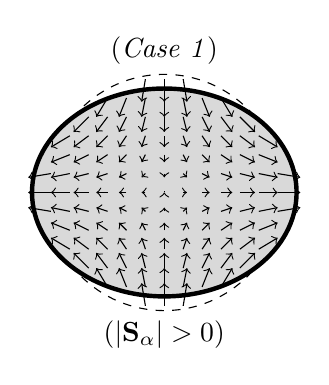
\begin{tikzpicture}[ultra thick,scale=0.6]
        \def\nRows{6}
        \def\nCols{6}
        \draw[dashed,thin] (0,0)circle(2.5);
        \draw[fill=gray!30] (0,0)ellipse(2.8 and 2.2);
        \foreach \x in {-\nRows,...,\nRows} {
            \foreach \y in {-\nCols,...,\nCols} {
                \pgfmathsetmacro\distance{veclen(\x*0.4, \y*0.4)};
                \pgfmathparse{\distance < 2.45 ? "blue" : "white"}
                \edef\colour{\pgfmathresult};
                \ifthenelse{\equal{\colour}{blue}}{                    
                    \draw[thin,->](\x*0.4,\y*0.4)--++(0.08*\x,-0.08*\y);
                }
            }
        }
        \node (txt) at (0,3){(\textit{Case 1})};
        \node (txt) at (0,-3){($|\textbf{S}_\alpha| > 0$)};
    \end{tikzpicture}
     \hfill
    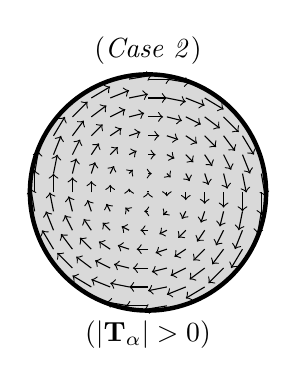
\begin{tikzpicture}[ultra thick,scale=0.6]
        \def\nRows{6}
        \def\nCols{6}
        \draw[fill=gray!30] (0,0)circle(2.5);
        \foreach \x in {-\nRows,...,\nRows} {
            \foreach \y in {-\nCols,...,\nCols} {
                \pgfmathsetmacro\distance{veclen(\x*0.4, \y*0.4)};
                \pgfmathparse{\distance < 2.5 ? "blue" : "white"}
                \edef\colour{\pgfmathresult};
                \ifthenelse{\equal{\colour}{blue}}{                    
                    \draw[thin,->](\x*0.4,\y*0.4)--++(0.08*\y,-0.08*\x);
                }
            }
        }
        \node (txt) at (0,3){(\textit{Case 2})};
        \node (txt) at (0,-3){($|\textbf{T}_\alpha| > 0$)};
    \end{tikzpicture}
    \hfill
    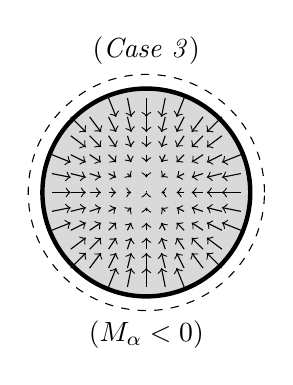
\begin{tikzpicture}[ultra thick,scale=0.6]
        \def\nRows{6}
        \def\nCols{6}
        \draw[dashed,thin] (0,0)circle(2.5);
        \draw[fill=gray!30] (0,0)circle(2.2);
        \foreach \x in {-\nRows,...,\nRows} {
            \foreach \y in {-\nCols,...,\nCols} {
                \pgfmathsetmacro\distance{veclen(\x*0.4, \y*0.4)};
                \pgfmathparse{\distance < 2.3 ? "blue" : "white"}
                \edef\colour{\pgfmathresult};
                \ifthenelse{\equal{\colour}{blue}}{                    
                    \draw[thin,->](\x*0.4,\y*0.4)--++(-0.08*\x,-0.08*\y);
                }
            }
        }
        \node (txt) at (0,3){(\textit{Case 3})};
        \node (txt) at (0,-3){($M_\alpha < 0$)};
    \end{tikzpicture}
    \hfill
    \caption{Graphical representation of the inner kinematics of an arbitrary particle under three scenarios. 
        The arrows represent the velocity field inside the particle, $\textbf{w}_d^0$, with the corresponding value of the moment of momentum tensor indicated below. 
        The operator $|\ldots|$ refers to the norm of the tensors. 
        According to the inner velocity field:
        (\textit{Case 1}) The particle experiences a mean rate of deformation, resulting in non-zero stretching of momentum along the principal axis of deformation;
        (\textit{Case 2}) The particle is rotating, leading to a non-zero angular momentum vector in the direction of rotation;
        (\textit{Case 3}) The particle undergoes compression, resulting in a negative trace of the moment of momentum.
    }
    \label{eq:scheme}
\end{figure}

% \subsection{Conservation laws}



% \subsubsection{Inside the volume}

 


% Let us consider the specific case of the momentum balance, i.e. $q_\alpha = \textbf{p}_\alpha$.
% In this situation, \ref{eq:dt_q_alpha} reads
% \begin{equation}
%     \ddt  \textbf{p}_\alpha
%     = \intO{ \rho_d\textbf{g} }
%     + \intS{ 
%         \left[
%         f_d^0 (\textbf{u}_I^0-\textbf{u}_d^0)
%          + \bm{\sigma}_d^0%\cdot\textbf{n}_d  
%         %+ \mathbf{\Phi}_d^0 
%         \right] 
%         \cdot \textbf{n}_d },
% \end{equation}
% first term reads as $\intO{ \rho_d\textbf{g} }$ 
% The first term on the right-hand side represents the total weight acting on the particle $\alpha$, 
% the second term represents the total source of momentum due to phase transfer, and it is expressed as, $\intS{ \rho_d \textbf{u}_d^0 (\textbf{u}_I^0-\textbf{u}_d^0)\cdot\textbf{n}_d }$,
% and the last term $\intS{ \bm{\sigma}_d^0\cdot\textbf{n}_d }$, represents the resultant of the hydrodynamic forces acting on the surface of the particle.
% It is important to notice that under this form, the exchange terms are expressed as integrals of dispersed phase fields denoted by the subscript $_d$.
% Nevertheless, depending on the nature of the dispersed phase, these fields may not always be defined.
% For rigid particles the stress within the particle $\bm{\sigma}_d^0$ is indeterminate \citep{guazzelli2011}.  
% Hence, our objective is to express these exchange terms, in terms of the continuous phase field quantities instead of the dispersed phase fields, i.e. in terms of $\mathbf{\Phi}_f^0$ and $\textbf{u}_f^0$ rather than $\mathbf{\Phi}_d^0$ and $\textbf{u}_d^0$. 

%\subsubsection{On the interfaces}
 

%For completeness, we exposed in \ref{ap:particles_eq} a clear derivation of the mass, momentum and total energy equations for a single particle.
%The derivation takes place using the same hypothesis as it is exposed in \ref{ap:hypothesis}.
%Especially, it is shown that the integration of the kinetic energy jump condition corresponds to the Lagrangian derivative of the particle surface, see \ref{eq:int_u_I2}.

 \section{Lagrangian equation for a single particle}
\label{ap:particles_eq}
\tb{MAYBE EXPLICITE A BIT MORE THE BOUNDARY FOR ENERRGY}
Following the same assumption as in \ref{sec:local_eq}, i.e. we consider no mass transfer and weightless interfaces, the Lagrangian  mass, momentum and energy equations for a single particle can be derived using the generic form \ref{eq:dt_q_alpha_tot} and reads as, 
\begin{align}
    \label{eq:dt_m_alpha}
    \ddt m_\alpha
    &= 
    0\\
    \label{eq:dt_p_alpha}
    \ddt (m_\alpha \textbf{u}_\alpha)
    &= 
    m_\alpha\textbf{g}
    +  \intS{\bm{\sigma}_1^0 \cdot \textbf{n}_2}\\
    \label{eq:dt_E_alpha_tot}
    \ddt (m_\alpha E_\alpha^\text{tot})
    &= 
    m_\alpha \textbf{u}_\alpha \cdot \textbf{g}
    +\textbf{u}_\alpha \cdot \intS{\bm{\sigma}_1^0 \cdot \textbf{n}_2}
    +\intS{\textbf{w}_1^0 \cdot \bm{\sigma}_1^0 \cdot  \textbf{n}_2} 
    - \intS{\textbf{q}_1^0 \cdot \textbf{n}_2}
\end{align}
where  $\intS{  \bm{\sigma}_1^0 \cdot \textbf{n}_2 }$ is the resultants of the hydrodynamic force and $\intS{ \textbf{q}_1^0 \cdot \textbf{n}_2 }$ is the resultants of the surface heat flux. 
The second term on the right hands side of the energy equation is the work produced by the mean force and the translational motion of the droplets, while $\intS{\textbf{w}_1^0 \cdot \bm{\sigma}_1^0 \cdot  \textbf{n}_2}$ is the work produced by the local forces and local motion of the fluid at the surface of the particle.
Since we integrated the energy over the particle's volume and its surface, we explicitly made appear the surface energy $\gamma s_\alpha$ within the derivative operator. 
Note that these equations does not explicitly account for inter-particle interactions. 
However, it is possible to include manually such forces by noticing that the surface external stress flux $\bm{\sigma}_1^0$ is the sum of hydrodynamic and particles-particles interaction forces, regardless it is pure contact forces from direct contact or a force mediated through the carrier fluid.
From this consideration it is possible to split every term involving the stress $\bm{\sigma}_1^0$ into two terms representing these contributions. 
Same comments can be made for the heat flux $\textbf{q}_1^0$. 
Although this distinction is important, for purpose of clearly we will stay general, and we will keep the fluxes $\bm{\sigma}_1^0$ and $\textbf{q}_1^0$ as such. 

In the spirit of the energy decomposition exposed in \ref{eq:E_alpha_def} the total energy equation can be split into three equations, one for the center of mass kinetic energy, internal motion and internal kinetic energy, namely,  
\begin{align}
    \label{eq:dt_u2_alpha}
    \frac{1}{2}\ddt (m_\alpha u_\alpha^2)
    &= 
    \textbf{u}_\alpha\cdot
    \textbf{g}m_\alpha
    + 
    \textbf{u}_\alpha\cdot
    \intS{\bm\sigma_1^0 \cdot \textbf{n}_2},\\
    \label{eq:dt_w2_alpha}
    \ddt (W_\alpha + \gamma s_\alpha)
    &= 
    \intS {\textbf{w}_1^0 \cdot \bm{\sigma}_1^0 \cdot \textbf{n}_2 }
    - \intO{ \bm{\sigma}_2^0 : \grad\textbf{u}_2^0 }
    \\
     \label{eq:dt_e_alpha}
    \ddt (m_\alpha e_\alpha )
    &= 
     \intO{ \bm{\sigma}_2^0 : \grad\textbf{u}_2^0  }
    -  \intS{\textbf{q}_1^0\cdot \textbf{n}_2 } 
\end{align}
respectively. 
The first equation is obtained by taking the dot product of \ref{eq:dt_p_alpha} with $\textbf{u}_\alpha$. 
The third equation is directly obtained using the local conservation of $e_k^0$ (\ref{eq:dt_rhoe_k}) and setting $f_2^0 = e_2^0$ in \ref{eq:dt_q_alpha_tot}.
The last equation is then obtained by subtracting the first and third equations to \ref{eq:dt_E_alpha_tot}. 
Note that in \citet{eq:dt_w2_alpha} the use of \ref{eq:dt_rhoI_uI2} makes appear explicitly the derivative of the surface energy $s_\alpha \gamma$. 
Note that under this form we see that the energy loss in the deformation represented by $W_p$ will be gathered in the surface energy which will in turn act as a source term in the internal kinetic energy motion.
The surface tension plays the role as a spring in the energy balance.   
From this set of equation we can easily see that the rate of dissipation terms $\intS{\bm{\sigma}_2^0 : \grad\textbf{u}_2^0}$ represent an energy sink in the equation of $W_\alpha$ while it is a source term in the internal energy equation. 
As it has been observed in the previous section, this terms convert the energy of internal motion to molecular agitation. 
However, the interplay between the center of mass  kinetic energy and the internal fluctuation is not obvious and has no common term with the heat and internal kinetic energy equation.
In fact, we will see that the transfer between these scales is archived thought the fluid phase pseudo turbulent energy. 


\section{Averaged two-fluid model}
\label{ap:two-fluid_model}
Before introducing the \textit{hybrid model} which will be the subject of the next section, we expose in the first place the classic averaged two-fluid model. 

\subsection{Averaged volume equations}
Using the generic formulation \ref{eq:avg_dt_chi_f} and the local expression of the mass, momentum and total energy equation, i.e. : \ref{eq:dt_rho}, \ref{eq:dt_rhou_k} and \ref{eq:dt_rhoE_k} we easily find the averaged form of the mass, momentum and total energy equation.
They read, 
\begin{align}
    \label{eq:dt_avg_rho_k}
    \pddt (\phi_k \rho_k)  
    + \div (
        \phi_k \rho_k\textbf{u}_k
    )
    &= 
    0,\\
    \label{eq:dt_avg_rhou_k}
    \pddt (\phi_k \rho_k\textbf{u}_k)  
    + \div (
        \phi_k \rho_k\textbf{u}_k\textbf{u}_k
        + \bm{\sigma}_k^\text{eq}
    )
    &= 
    \phi_k \rho_k \textbf{g} 
    +  \avg{\delta_I \bm{\sigma}_k^0 \cdot \textbf{n}_k},\\
    \label{eq:dt_avg_rhoE_k}
    \pddt (\phi_k\rho_kE_k)  
    + \div (
        \phi_k\rho_kE_k\textbf{u}_k
        + \bm{q}_k^\text{eq}
        + \textbf{u}_k \cdot \bm{\sigma}_k^\text{eq}
        % - \textbf{u}_k^0 \cdot \bm{\sigma}_k^0 
        % + \textbf{q}_k^0
        )
    &= 
    \phi_k \rho_k\textbf{u}_k \cdot \textbf{g} 
    + \avg{\delta_I (\textbf{u}_k^0 \cdot \bm{\sigma}_k^0 - \textbf{q}_k^0)\cdot \textbf{n}_k},
\end{align} 
respectively. 
Where we have introduced the effective stress and heat fluxes namely, 
\begin{align*}
    &\bm{\sigma}_k^\text{eq}
    = 
     \rho_k\avg{\chi_k \textbf{u}_k'\textbf{u}_k'}
      - \phi_k \bm{\sigma}_k,%- n_p \textbf{M}_p
    &\textbf{q}_k^\text{eq}
    =\textbf{q}_k^\text{e} +\textbf{q}_k^\text{k},  \\
    &\textbf{q}_k^\text{e}
    = \rho_k \avg{\chi_k\textbf{u}_k' e_k'} 
    + \phi_k\textbf{q}_k,
    &\textbf{q}_k^\text{k}
    = \rho_k \avg{\chi_k \textbf{u}_k' k_k} 
    - \avg{\chi_k \textbf{u}_k' \cdot \bm{\sigma}_k^0}.
\end{align*}
The main differences between these equations and their microscale counterpart, is that : 
(1) we have introduced a pre factor $\phi_k$ in front of most the unknown  ($\textbf{u}_k$ and $E_k$), 
(2) the non-convective fluxes appear under the form of an effective tensor containing the covariance of the quantity to be conserved with the local velocity of the phase, 
and (3) a new source term appear on the RHS accounting for the exchange across the phases. 
Additionally, it is interesting to notice that the effective fluxes of the total energy is written as the mean work done by the effective stress of the momentum $\textbf{u}_k \cdot \bm{\sigma}_k^\text{eq}$ plus an effective heat flux $\bm{q}_k^\text{eq}$. 

The terms $\avg{\chi_k \textbf{u}_k'\textbf{u}_k'}$ will be referred as the Reynolds stress or pseudo turbulent stress. 
It has a fundamental importance in the multiphase flow problem as it appear in \ref{eq:dt_avg_rhou_k} and as we see now its trace is related to the mean kinetic energy. 
Indeed, the phase averaged total energy can be further decompose into three energy components, that is,  
\begin{align}
    E_k = e_k + k_k + u_k^2/2
    \label{eq:E_def2}
\end{align}
where $k_k$ is the pseudo-turbulent kinetic energy defined as, $\phi_k k_k = \frac{1}{2}\avg{\chi_k \textbf{u}_k'\cdot \textbf{u}_k'}$. 
Each of the components of the total energy represent the averaged agitation at different scales. 
From molecular agitation which quantified by $e_k$, to the macroscopic scale agitation or kinematic energy $u_k^2$, and in between we find the pseudo turbulent energy $k_k$ which represents the local scale velocity fluctuation. 
To fully describe the averaged total energy one must add at least a supplementary equation either for $k_k$ or $e_k$ assuming \ref{eq:dt_avg_rhoE_k} is solved. 
Using \ref{eq:dt_avg_rhou_k} dotted with $\textbf{u}_k$ yields an equation for the mean kinetic energy. 
Averaging \ref{eq:dt_rhoe_k} yields un equation for $e_k$.  
Then, subtracting these two equations to \ref{eq:dt_avg_rhoE_k} gives us an equation for $k_p$. 
The kinetic energy, pseudo turbulent and internal averaged equations are, 
\begin{align}
    \label{eq:dt_avg_uk2}
    &\pddt (\phi_k \rho_ku_k^2/2)  
    + \div (
        \phi_k \rho_k\textbf{u}_ku_k^2/2
        + \textbf{u}_k \cdot \bm{\sigma}_k^\text{eq}
    )
    = 
    \bm{\sigma}_k^\text{eq} : \grad \textbf{u}_k
    + \phi_k \rho_k \textbf{u}_k\cdot \textbf{g} 
    +  \textbf{u}_k\cdot \avg{\delta_I \bm{\sigma}_k^0 \cdot \textbf{n}_k},\\
    \label{eq:dt_avg_kk}
    &\pddt (\phi_k\rho_kk_k)  
    + \div (
        \phi_k\rho_kk_k\textbf{u}_k
        + \textbf{q}_k^\text{k} 
        )
    = 
    - \avg{\chi_k\bm{\sigma}_k^0 : \grad \textbf{u}_k^0}
    - \bm{\sigma}_k^\text{eq} : \grad \textbf{u}_k
    + \avg{\delta_I \textbf{u}_k' \cdot \bm{\sigma}_k^0 \cdot \textbf{n}_k},\\
    \label{eq:dt_avg_ek}
    &\pddt (\phi_k\rho_ke_k)  
    + \div (
        \phi_k \rho_ke_k\textbf{u}_k
        +
        \textbf{q}_k^\text{e} 
        )
    = 
    \avg{\chi_k\bm{\sigma}_k^0 : \grad \textbf{u}_k^0}
    - \avg{\delta_I \textbf{q}_k^0 \cdot \textbf{n}_k},
\end{align}
respectively. 
This derivation is in agreement with \citet{morel2015mathematical}. 
Under this form the energy transfer across scale is clear. 
Indeed, the term $\bm{\sigma}_k^\text{eq} : \grad \textbf{u}_k$ act as a sink term in \ref{eq:dt_avg_uk2} and a source term in \ref{eq:dt_avg_kk}, while the averaged diffusive terms $\avg{\chi_k\bm{\sigma}_k^0 : \grad \textbf{u}_k^0}$ is a sink in \ref{eq:dt_avg_kk} and a source in \ref{eq:dt_avg_ek}. 
To determine the total energy only two of the four energy equations must be solved. 
In practice, it is useful to solve one equation for $k_k$ since it is useful for the Reynolds stress modeling since $\avg{\chi_k \textbf{u}_k^0 \textbf{u}_k^0}: \bm\delta = 2 k_k$, and another for $e_k$ since $u_k^2$ is already determined by the momentum equation. 

\subsection{Averaged surface equations}
The volume averaged equations must be completed by an averaged surface transport equation.  
For this purpose we multiply \ref{eq:surface_tension}, \ref{eq:dt_rhoIe_I} and \ref{eq:dt_rhoI_uI3} by $\delta_I$ and apply the average operator.
By considering the topological equations we obtain the  momentum, kinetic and internal energy averaged surface equations, namely
\begin{align}
    \label{eq:dt_avg_uI}
    \avg{\delta_I \Jump{\bm{\sigma}^0_k}}
    &= -\gamma \div \avg{\delta_I (\bm\delta - \textbf{nn})},\\
    \label{eq:dt_avg_gamma}
    \avg{\delta_I \Jump{\textbf{u}_k^0 \cdot \bm{\sigma}^0_k}}
    &= - \gamma \left[
        \pddt \phi_I
        +  \div \avg{\delta_I (\textbf{u}_{I}^0 \cdot \textbf{n})\textbf{n} },
    \right]\\
    \avg{\delta_I \Jump{\textbf{q}^0_k}}
    &= 0
\end{align}
respectively. 
The first equation represents the contribution of the surface tension stresses to the bulk momentum equation.
The second equation represents the amount of energy stored as surface deformation.
And the last equation witnesses of the continuity of heat flux through the interface. 

\subsection{Averaged single fluid formulation}
Lastly, by summing the above formulations we can also derive equations for the bulk quantities. 
Indeed, summing \ref{eq:dt_avg_rho_k}, \ref{eq:dt_avg_rhou_k} and \ref{eq:dt_avg_rhoE_k} for $k=f,d$ with the surface equations one obtain the bulk conservation equations, 
\begin{align}
    \label{eq:dt_avg_rho}
    \pddt \rho 
    + \div (
         \rho \textbf{u}_m
    )
    &= 
    0,\\
    \label{eq:dt_avg_rhou}
    \pddt ( \rho\textbf{u}_m)  
    + \div (
         \rho\textbf{u}_m\textbf{u}_m
        + \bm{\sigma}^\text{eq}_m
    )
    &= 
     \rho \textbf{g} \\
    \label{eq:dt_avg_rhoE}
    \pddt (\rho E_m)  
    + \div (
        \rho E_m \textbf{u}_m
        + \bm{q}^\text{eq}_m
        + \textbf{u}_m \cdot \bm{\sigma}^\text{eq}_m
        % - \textbf{u}_k^0 \cdot \bm{\sigma}_k^0 
        % + \textbf{q}_k^0
        )
    &= 
     \rho \textbf{u}_m  \cdot \textbf{g} 
\end{align} 
respectively. 
Where we have introduced the effective stress and heat fluxes namely, 
\begin{align*}
    &\bm{\sigma}^\text{eq}_m
    = 
    \avg{ \rho^0\textbf{u}'_m\textbf{u}'_m}
      - \phi_f\bm\sigma_f
      - \phi_d\bm\sigma_d
      - \phi_I\bm\sigma_I,%- n_p \textbf{M}_p
    &\textbf{q}^\text{eq}_m
    =\textbf{q}^\text{e}_m +\textbf{q}^\text{k}_m,  \\
    &\textbf{q}^\text{e}_m
    = \avg{\rho^0\textbf{u}_m' e_m'} 
    + \phi\textbf{q}_m,
    &\textbf{q}^\text{k}_m
    = \avg{\rho^0 \textbf{u}_m' k_m} 
    - \avg{ \textbf{u}_m' \cdot \bm{\sigma}^0}.
\end{align*}
In these equations we have make use of the subscript $_m$ to denote the Favre average quantities, such that, 
\begin{align*}
    \rho \textbf{u}_m
    = \avg{\rho^0 \textbf{u}^0}
    &&
    \rho E_m
    = \avg{\rho^0 \textbf{u}^0}
    &&
    \rho e_m
    = \avg{\rho^0 \textbf{u}^0}
\end{align*}
Likewise, the fluctuating quantity are written as, 
\begin{equation}
    \textbf{u}_m'
    = \textbf{u}^0 - \textbf{u}_m.
\end{equation}
In \ref{eq:dt_avg_rhoE} we have defined the bulk total energy as the average of the sum of the local energy, namely, 
\begin{equation}
    \rho E_m = \avg{\sum_k \rho_k [e_k^0 + \frac{1}{2}(u_k)^2] 
    + \delta_I \gamma}
    = \rho( e_m +  k_m + \frac{1}{2}u_m^2)
\end{equation}
with, $e_m = \avg{\sum_k \rho_k\phi_k e_k + \phi_I \gamma}$ and $k = \avg{\rho^0 \textbf{u}'\cdot \textbf{u}'}/2$. 


These equations are particularly interesting from an experimental point of view. 
% Indeed, as in experiment we cannot distinguish between the details of both phase. 
For example in a Rheometer we are able to measure only for the \textit{Bulk stress} $\bm\sigma^\text{eq}_m$ and not $\bm\sigma^\text{eq}_f$ and $\bm\sigma^\text{eq}_d$ separately, as it measure the stress response from the mixture phases. 
Therefore, it is of interest to describe a bit more in details the \textit{Bulk stress}, which is the subject of the next section.


\subsection{The bulk stress in dispersed multiphase flow}


Now that the architecture of the averaged dispersed multiphase flow equation is clarified, we would like to present the expression of the bulk stress tensor in a suspension of inertial particles subject to an arbitrary local body force field, $\textbf{b}^0$.
Firstly, is important to recall the definition of the \textit{bulk stress}. 
We define the \textit{bulk stress} tensor as a force applied on the fluid and on the particles phase, having the form $\div \bm{\Sigma}$, which added to the total external force $\textbf{B}$, balance exactly the material derivative of the mixture momentum : $\frac{D \rho \textbf{u}}{Dt}$. 
In this definition $\textbf{B}$ cannot be decomposed into a vector and a divergence of a tensor, in which case the latter would just contribute to $\bm{\Sigma}$.
Equally, we insist on the fact that the momentum considered is $\rho\textbf{u}$ which is the bulk momentum. 

We first expose the averaged mixture momentum and angular momentum equation easily derived from \ref{eq:dt_avg_f}, 
\begin{align}
    \pddt (\rho u_i)
    + \partial (\rho u_iu_k
    + \sigma_{ik}^\text{eq})
    = b_i\\
    \epsilon_{ijk} \sigma_{jk}
    = 0 
    \label{eq:momentum_bulk}
\end{align}
In the momentum equation we have defined, $\sigma_{ik}^\text{eq} = \avg{\rho\textbf{u}'\textbf{u}'}
- \avg{\chi_1\bm{\sigma}_1^0}-\avg{\chi_2\bm{\sigma}_2^0} - \avg{\delta_I \bm{\sigma}_I^0}$. 
Additionally, in the averaged angular momentum equation we have assumed that no-body torque exist at the local scale making the second equality equal to $0$ \citet{leal2007advanced} and the averaged mixture stress $\bm{\sigma}$ a symmetric quantity. 
However, note that $\bm{\sigma}$ is not exactly equal to the \textit{bulk stress} tensor $\bm{\Sigma}$ since $\textbf{b}$ can be expressed as a divergence of a stress.
Indeed, have defined $\textbf{b} = \textbf{B} + \div  \pMOavg{\textbf{b}_2^0}$ where $\textbf{B} = \phi_1 \textbf{b}_1 +  \pOavg{\textbf{b}_2^0 }$ and  $\pMOavg{\textbf{r}\textbf{b}_2^0}$ is defined accordingly to the previous definition. 
It follows the definition of the \textit{bulk stress} : 
\begin{equation}
    \bm{\Sigma}
    = 
    \avg{\rho\textbf{u}'\textbf{u}'}
    - \avg{\chi_1\bm{\sigma}_1^0}
    - \avg{\chi_2\bm{\sigma}_2^0} 
    - \avg{\delta_I \bm{\sigma}_I^0}
    - \pMOavg{\textbf{r}\textbf{b}_2^0}
\end{equation}
which proves already, in the absence of particles moments of the body forces $\pMOavg{\textbf{r}\textbf{b}_2^0}$, the antisymmetric part of the suspension stress is null, in agreement with \citet{dolata2020heterogeneous}.
% This skew symmetric part can be written in vector form as, 
% \begin{equation*}
%     \epsilon_{ijk}\textbf{T}_{jk}
%     = 
%     -\epsilon_{ijk} \pOavg{r_kb_j}
%     -\epsilon_{ijk}\frac{1}{2}\partial_l \pOavg{r_lr_kb_j}
%     = 0  
% \end{equation*}
We recall that the carrier fluid is a Newtonian fluid, therefore we may express the fluid phase stress as, 
\begin{equation}
    \phi_1 \sigma_{1,jk}
    = -p_1 \delta_{jk}
    + \mu_1 e_{jk}
    - \mu_1 \phi_2 e_{2,jk}. 
\end{equation} 
Additionally, we use the methodology of \citep{lhuillier1992volume,lhuillier1996contribution} to re express the averaged particle stress terms. 
The divergence of the particle phase stress may be expressed using \ref{eq:f_exp}, 
\begin{align}
    \label{eq:exp_sigma22}
    \partial_k \avg{\chi_2 {\sigma}_2^0}_{ik}
    &=  \partial_k\pOavg{ {\sigma}_{2,ik}^0}
    -\frac{1}{2} \partial_k\partial_j
    \pOavg{ r_j{\sigma}^0_{2,ik} + r_k\sigma^0_{2,ij}}
    + \ldots  \\
    \label{eq:exp_sigmaI2}
    \partial_k \avg{\delta_I {\sigma}^0_I}_{ik} 
    &=  \partial_k\pSavg{ {\sigma}_{I,ik}^0 }
        -\frac{1}{2} \partial_k\partial_j \pSavg{ r_j {\sigma}_{I,ik}^0+r_k {\sigma}_{I,ij}^0 }
        + \ldots  
\end{align}
Note that the heterogeneous terms must remain symmetric in the index $kj$ due to the double contraction with the operator $\partial_k\partial_j$, thus only the symmetric part in $jk$ remain and the terms such as, $\pOavg{ r_j{\sigma}^0_{2,ik} - r_k\sigma^0_{2,ij}}$ vanish. 
Upon the use of the moment of momentum equation of the first and second order we can easily derive these expressions, 
\begin{align}
    \intS{ (\bm{\sigma}_I)_{ik}}
    +\intO{ (\bm{\sigma}_2^0)_{ik}}
    = 
    \intO{ \rho_2 
    (\textbf{w}_2^0\textbf{w}_2^0  )_{ik}
    }
    -\ddt \intO{ r_i (\textbf{u}^0_2)_k }
    +\intS{ 
        b_{i}
        r_k 
    }
    +\intS{ 
     r_i (\bm{\sigma}_1^0 \cdot \textbf{n}_2)_{k}
    }\\
    \intO{ r_{j}(\bm{\sigma}^0_2)_{ik}+r_{k}(\bm{\sigma}^0_2)_{ji}}
    +\intS{ r_{j}(\bm{\sigma}^0_I)_{ik}+r_{k}(\bm{\sigma}_I^0)_{ji}}
    = 
    - \ddt\intO{ \rho_2 (\textbf{u}_2^0)_i r_j r_k }\nonumber\\
    + \intO{ \rho_2 (r_{j} (\textbf{w}_2^0)_k (\textbf{u}^0_2)_i + r_k (\textbf{w}_2^0)_j (\textbf{u}^0_2)_i)}
    +\intS{  r_{k}r_{j} (\bm{\sigma}_1^0)_{il} (\textbf{n}_2)_l }
    + \intO{ r_{k}r_{j}  \rho_2 b_i } 
    \label{eq:dt_P2_alpha}
\end{align}
It is evident that by using an arbitrary order of moment of momentum equation one can substitute any volume integral of the particle stress appearing in the expansion \ref{eq:exp_sigma22}. 
% By consideration of symmetric of the local stress, it is evident that the skew symmetric part of the moment of momentum will not have any dynamical role thus we can retrieve the average of \ref{eq:dt_mu_alpha} to the first relation. 
% To extract the skew symmetric part we start by writing the permutation of these equations with $ik$ yielding,  
% \begin{align}
%     \intS{ 
%     (\bm{\sigma}_I)_{ki}
%     }
%     +\intO{ 
%     (\bm{\sigma}_2^0)_{ki}
%     }
%     = 
%     \intO{ \rho_2 
%     (\textbf{w}_2^0\textbf{w}_2^0  )_{ki}
%     }
%     -\ddt \intO{ r_k (\textbf{u}^0_2)_i }
%     +\intS{ b_{k}r_i }
%     +\intS{ r_k (\bm{\sigma}_1^0 \cdot \textbf{n}_2)_{i}}\\
%     \intO{ r_{j}(\bm{\sigma}^0_2)_{ki}+r_{i}(\bm{\sigma}^0_2)_{jk}}
%     +\intS{ r_{j}(\bm{\sigma}^0_I)_{ki}+r_{i}(\bm{\sigma}_I^0)_{jk}}
%     = 
%     - \ddt\intO{ \rho_2 (\textbf{u}_2^0)_k r_j r_i }\nonumber\\
%     + \intO{ \rho_2 (r_{j} (\textbf{w}_2^0)_i (\textbf{u}^0_2)_k + r_i (\textbf{w}_2^0)_j (\textbf{u}^0_2)_k)}
%     +\intS{  r_{i}r_{j} (\bm{\sigma}_1^0)_{kl} (\textbf{n}_2)_l }
%     + \intO{ r_{i}r_{j}  \rho_2 b_k } \\
%     \intO{ r_{i}(\bm{\sigma}^0_2)_{jk}+r_{k}(\bm{\sigma}^0_2)_{ij}}
%     +\intS{ r_{i}(\bm{\sigma}^0_I)_{jk}+r_{k}(\bm{\sigma}_I^0)_{ij}}
%     = 
%     - \ddt\intO{ \rho_2 (\textbf{u}_2^0)_j r_i r_k }\nonumber\\
%     + \intO{ \rho_2 (r_{i} (\textbf{w}_2^0)_k (\textbf{u}^0_2)_j 
%     + r_k (\textbf{w}_2^0)_i (\textbf{u}^0_2)_j)}
%     +\intS{  r_{k}r_{i} (\bm{\sigma}_1^0)_{jl} (\textbf{n}_2)_l }
%     + \intO{ r_{k}r_{i}  \rho_2 b_j } 
% \end{align}
% Acknowledgement of the symmetrical nature of $\bm{\sigma}_2^0$ and $\bm{\sigma}_I^0$ gives the following antisymmetrical balance equations, 
% \begin{align}
%     0
%     = 
%     -\ddt \intO{ r_i (\textbf{u}^0_2)_k -r_k (\textbf{u}^0_2)_i }
%     +\intS{ b_{i}r_k -b_{k}r_i }
%     +\intS{r_i (\bm{\sigma}_1^0 \cdot \textbf{n}_2)_{k} - r_k (\bm{\sigma}_1^0 \cdot \textbf{n}_2)_{i}}\\
%     \intO{ r_{j}(\bm{\sigma}^0_2)_{ik}
%             -r_{i}(\bm{\sigma}^0_2)_{jk}}
%     +\intS{ r_{j}(\bm{\sigma}^0_I)_{ik}
%            - r_{i}(\bm{\sigma}_I^0)_{jk}}
%     = 
%     - \ddt\intO{ \rho_2 (\textbf{u}_2^0)_i r_j r_k -  \rho_2 (\textbf{u}_2^0)_j r_i r_k }\nonumber\\
%     + \intO{ \rho_2 (r_{j} (\textbf{w}_2^0)_k (\textbf{u}^0_2)_i + r_k (\textbf{w}_2^0)_j (\textbf{u}^0_2)_i)}
%     - \intO{ \rho_2 (r_{i} (\textbf{w}_2^0)_k (\textbf{u}^0_2)_j + r_k (\textbf{w}_2^0)_i (\textbf{u}^0_2)_j)}\\
%     +\intS{  r_{k}r_{j} (\bm{\sigma}_1^0)_{il} (\textbf{n}_2)_l 
%     -r_{k}r_{i} (\bm{\sigma}_1^0)_{jl} (\textbf{n}_2)_l }
%     + \intO{ r_{k}r_{j}  \rho_2 b_i
%     - r_{k}r_{i}  \rho_2 b_j } 
% \end{align}
% The last equation need to be added to the second permutation which gives, 
% \begin{align*}
% \intO{ r_{j}(\bm{\sigma}^0_2)_{ik}}
% +\intS{ r_{j}(\bm{\sigma}^0_I)_{ik}}
% = 
% - \ddt\intO{ \rho_2 (\textbf{u}_2^0)_k r_j r_i 
% + \rho_2 (\textbf{u}_2^0)_i r_j r_k 
% -  \rho_2 (\textbf{u}_2^0)_j r_i r_k }\nonumber\\
% + \intO{ \rho_2 (r_{j} (\textbf{w}_2^0)_k (\textbf{u}^0_2)_i + r_k (\textbf{w}_2^0)_j (\textbf{u}^0_2)_i)}
% - \intO{ \rho_2 (r_{i} (\textbf{w}_2^0)_k (\textbf{u}^0_2)_j + r_k (\textbf{w}_2^0)_i (\textbf{u}^0_2)_j)}\\
% - \intO{ \rho_2 (r_{j} (\textbf{w}_2^0)_i (\textbf{u}^0_2)_k + r_i (\textbf{w}_2^0)_j (\textbf{u}^0_2)_k)}\\
% +\intS{  r_{k}r_{j} (\bm{\sigma}_1^0)_{il} (\textbf{n}_2)_l 
% +r_{j}r_{i} (\bm{\sigma}_1^0)_{kl} (\textbf{n}_2)_l 
% -r_{k}r_{i} (\bm{\sigma}_1^0)_{jl} (\textbf{n}_2)_l }
% + \intO{ r_{k}r_{j}  \rho_2 b_i
% + r_{j}r_{i}  \rho_2 b_k 
% - r_{k}r_{i}  \rho_2 b_j 
% } 
% \end{align*}
In, addition one must notice that the particle angular momentum balance equation doesn't involve the integral of the particle local stress and has therefore, no dynamical role in the equivalent stress expression. 
Making use of these remarks we obtain this general formula for the suspension stress,  
\begin{multline}
    \bm{\Sigma}
    = \avg{\rho\textbf{u}'\textbf{u}'}_{ik}
    + \phi_1 p_1 \delta_{ik}
    - \mu_1 e_{ik}
    % + \mu_1 \phi_2 e_{2,ik}. 
    - \pOavg{ \rho_2 (\textbf{w}_2^0\textbf{w}_2^0  )_{ik}}
    + \pavg{\ddt {\mathcal{S}_{ik}} }\\
    - \pSavg{ b_{i}r_k - b_{k}r_i }
    - \pSavg{ r_i (\bm{\sigma}_1^0 \cdot \textbf{n}_2)_{k}
    + r_k (\bm{\sigma}_1^0 \cdot \textbf{n}_2)_{i}}
    + \mu_1 \pOavg{e_2^0}_{ik}
    + \frac{1}{2} \div\bm{\Sigma}_1
    \label{eq:eq_stress}
\end{multline}
with the inhomogeneous stress gathered in $\bm{\Sigma}_1$, namely,
\begin{multline}
    \bm{\Sigma}_1
    = 
    - \pavg{\ddt\intO{ \rho_2 (\textbf{u}_2^0)_i r_j r_k }}
    + \pOavg{ \rho_2 (r_{j} (\textbf{w}_2^0)_k (\textbf{u}^0_2)_i + r_k (\textbf{w}_2^0)_j (\textbf{u}^0_2)_i)}\nonumber\\
    +\pSavg{  r_{k}r_{j} (\bm{\sigma}_1^0)_{il} (\textbf{n}_2)_l }
    - \mu_1 2 \pOavg{\textbf{r} \textbf{e}_2^0}_{jik}
\end{multline}
According to \ref{eq:scheme_equivalence}, expanding each component related to the dispersed phase in \ref{eq:momentum_bulk} one would see appear each moment of momentum equations under the divergence operator.
However, to stay consistent with the definition of the bulk stress tensor $\bm{\Sigma}$, we must keep the advecting term on the LHS of \ref{eq:momentum_bulk} unchanged, this is however not the case of the averaged body force term $\textbf{b}$ which allowed us to cancel all the body forces terms with the expansion of $\textbf{T}$.  

One of the major question in suspension dynamic raised by several authors, is the evaluation of the bulk stress or equivalent stress tensor of a suspension, see \citep{prosperetti2006stress, batchelor1970stress,zhang1997momentum,nadim1996concise} and more recently \citet{dolata2020heterogeneous}. 
The answer to this question is given in the general case of the generic averaged mixture equation. 
In light of \ref{eq:eq_stress} we have demonstrated how to express in a routine manner the bulk stress of the particle phase. 
And doing so without making appear explicitly the particles  internal stress. 
This, conclusion deserve several comments regarding previous studies. 
In  \citet{jackson1997locally},  the volume averaged momentum balance (equation (38) of \citet{jackson1997locally}) they make appear the higher moment of velocity of the particles as closure terms, these are hidden in $\pOavg{\textbf{w}_2^0 \textbf{w}_2^0}$.
However, in \citet{jackson1997locally} they did not remove the angular momentum to the stress yieldings a slightly different term. 
What we have shown here is that these higher moments of the particles phase such has the particles rotations have no dynamical significance in the mixture equations. 
Therefore, equation (38) of \citet{jackson1997locally} can be further simplified to the fluid and first order particle averaged equations. 
Equally, in the momentum mixture equation derived by \citet{zhang1997momentum} (equation (8.2)), they make appear explicitly the higher moment of acceleration and the higher moments of velocity in their equivalent stress. 
These terms must therefore simplify. 
In fact as, it could be supposed in their appendix these moments equally cancel. 
In agreement with \citet{dolata2021faxen} which also found that the only remaining part of the stress were solely the fluid phase exchange terms upon the calculation of the body forces moments. 
Similar, comments can be made on the study of \citet{prosperetti2006stress}. 
This also explain why \citet{nadim1996concise} found out that the interfacial terms of the surface tension and viscous interfacial forces play no direct role in the equivalent stress of the emulsion.

\section{Application}
\label{sec:application}
\section{Averaged equations}



Now that we reached a clear understanding of the mathematical structures of the averaged two-phase flow equations we now expose the averaged set of equations which constitute the \textit{Hybrid model}. 
In this section we consider the simplifying assumption exposed in \ref{ap:hypothesis}. 
As mentioned in \ref{sec:two-fluid} we derive the mass, momentum and energy for the particles and continuous phase. 
Additionally, to describe the particle shape and inner velocity, one must consider the second moment of mass and first moment of momentum averaged equations. 
This, makes a total of 10 equations, 6 for the particle phase and 4 for the continuous phase.

To support the subsequent discussion, we provide the expressions of the closure terms of a dilute emulsion of spherical droplets. 
We will consider a monodisperse suspension of droplets with radius $a$ and constant viscosity $\lambda \mu_f$. 
% Additionally, both phases are assumed Newtonian therefore, $\bm{\sigma}_k^0 = - p_k^0 \bm\delta + \mu_k \textbf{e}_k^0$, with $\textbf{e}_k^0 = \grad \textbf{u}_k^0+(\grad \textbf{u}_k^0)^\dagger$ the shear rate tensor, $\bm\delta$ the identity tensor and $p_k ^0$ the local pressure. 
It must be understood that our goal is not to derive a set of equations for non-inertial spherical particles, in which case the energy equations and first order moment equations would be unnecessary. 
Instead, we provide the closures in stokes flow regime to illustrate their physical implication. 
Thus, even though the closures are expressed in the Stokes limit, note that the set of equations provided remains valid regardless of the flow regime.


\subsection{Averaged equations}

In this section we derive and discuss the averaged equations governing the continuous and teh dispersed  phase. 

\subsubsection{Continuous phases}


The equations for the carrier fluid are basically the same as in the classic two-fluid model derived in \ref{ap:two-fluid_model}, except that the interfacial terms of the form $\avg{\delta_I \ldots }$ need to be reformulated.
Indeed, the interfacial terms must be reformulated in terms of particle-averaged quantities in order to be consistent with the particle-phase equations \citep{jackson1997locally,zhang1994averaged}. 
This is achieved through the use of \ref{eq:f_exp} which enables us to convert the exchange terms appearing in \ref{eq:avg_dt_chi_f} into a series expansion of particle phase quantities. 
For clarity, we only retain the first, second and sometime third order terms of this expansion. 
The continuous phase averaged mass, momentum and total energy equations yield, 
\begin{align}
    \label{eq:dt_hybrid_rho}
    &\pddt (\phi_f \rho_f)  
    + \div (
        \phi_f \rho_f\textbf{u}_f
    )
    = 
    0,\\
    \label{eq:dt_hybrid_rhou_f}
    &\pddt (\phi_f \rho_f\textbf{u}_f)  
    + \div (
        \phi_f \rho_f\textbf{u}_f\textbf{u}_f
        + \bm{\sigma}_f^\text{eq}
    )
    = 
    \phi_f \rho_f \textbf{g} 
    - \pSavg{{\bm{\sigma}_f^0 \cdot \textbf{n}_d}},
    % +\div  \pSavg{{\textbf{r}\bm{\sigma}_f^0 \cdot \textbf{n}_d}}
    \\
    \label{eq:dt_hybrid_rhoE_f}
    &\pddt (\phi_f\rho_fE_f)  
    + \div (
        \phi_f\rho_fE_f\textbf{u}_f
        + \bm{q}_f^\text{eq}
        + \textbf{u}_f \cdot \bm{\sigma}_f^\text{eq}
        % - \textbf{u}_f^0 \cdot \bm{\sigma}_f^0 
        % + \textbf{q}_f^0
        )
    = 
    \phi_f \rho_f\textbf{u}_f \cdot \textbf{g} 
    - \textbf{u}_p \cdot \pSavg{{\bm{\sigma}_f^0 \cdot \textbf{n}_d}}\nonumber \\
    &- \pavg{ \textbf{u}_\alpha' \cdot \intS{  \bm{\sigma}_f^0 \cdot \textbf{n}_d}}
    - \pavg{ \intS{\textbf{w}_d^0 \cdot \bm{\sigma}_f^0 \cdot \textbf{n}_d}}
    + \pSavg{{\textbf{q}_f\cdot \textbf{n}_d}},
    % &\div [    
        % \textbf{u}_p \cdot \pSavg{{ \textbf{r}\bm{\sigma}_f^0 \cdot \textbf{n}_d}}
    % + \pavg{ \textbf{u}_\alpha' \cdot \intS{ \textbf{r} \bm{\sigma}_f^0 \cdot \textbf{n}_d}}
    % + \pavg{ \intS{\textbf{r}\textbf{w}_d^0 \cdot \bm{\sigma}_f^0 \cdot \textbf{n}_d}}
    % - \pavg{ \intS{\textbf{r}  \textbf{q}_f^0 \cdot \textbf{n}_d}}
    % ]
\end{align} 
respectively. 
Where we have introduced the equivalent stress tensor $\bm{\sigma}_f^\text{eq}$ and equivalent energy flux $\textbf{q}^\text{eq}_f$ as,
\begin{align}
    \label{eq:sigma_eq_def}
    \bm{\sigma}_f^\text{eq}
    =& 
    \avg{\chi_f\rho_f\textbf{u}_f'\textbf{u}_f'}
    - \phi_f \bm{\sigma}_f%- n_p \textbf{M}_p
    - \pSavg{{\textbf{r}\bm{\sigma}_f^0 \cdot \textbf{n}_d}}
    +\frac{1}{2}\div \pSavg{{\textbf{rr}\bm{\sigma}_f^0 \cdot \textbf{n}_d}}
    + \ldots
    \\
    \textbf{q}_f^\text{eq}
    =&\textbf{q}_f^\text{e} +\textbf{q}_f^\text{k} \nonumber \\
    \textbf{q}_f^\text{e}
    =& \rho_f \avg{\chi_f \textbf{u}_f' e_f'} 
    + \phi_f\textbf{q}_f 
    +\pSavg{{\textbf{r}\textbf{q}_f^0 \cdot \textbf{n}_d}} 
    -\frac{1}{2}\div \pSavg{{\textbf{rr}\textbf{q}_f^0 \cdot \textbf{n}_d}} 
    + \ldots
    \\
    \textbf{q}_f^\text{k}
    =& \rho_f \avg{\chi_f \textbf{u}_f' k_f} 
    - \avg{\chi_f \textbf{u}_f' \cdot \bm{\sigma}_f^0}
    + (\textbf{u}_f - \textbf{u}_p)\cdot
    \pSavg{{\textbf{r}\bm{\sigma}_f^0 \cdot \textbf{n}_d}}
    \label{eq:q_f_k_def}
    \\\nonumber &
    - \pavg{ \textbf{u}_\alpha' \cdot \intS{ \textbf{r} \bm{\sigma}_f^0 \cdot \textbf{n}_d}}
    - \pavg{ \intS{\textbf{r}\textbf{w}_d^0 \cdot \bm{\sigma}_f^0 \cdot \textbf{n}_d}}
    + \div[\ldots]
\end{align}
It is clear that those equations yield essentially the same as the previous set of equations presented in \ref{ap:two-fluid_model}.
The only difference is the presence of additional terms inside $\bm{\sigma}^\text{eq}_f$ and $\textbf{q}^\text{eq}_f$ due to the expansion of the interfacial terms. 
The $[\ldots]$ in \ref{eq:sigma_eq_def} to \ref{eq:q_f_k_def} refers to the higher moments of the expansion of the interfacial terms that are not display here for purpose of clarity. 
The averaged continuous-phase momentum balance \eqref{eq:dt_hybrid_rhou_f} under its \textit{hybrid} form was established long ago by \citet{zhang1997momentum,jackson1997locally}.  
\ref{eq:dt_hybrid_rhou_f} is of course consistent with the formulation given by these authors.

Now, let us discuss the continuous-phase averaged total energy balance \eqref{eq:dt_hybrid_rhoE_f}. 
Most of the terms have already been addressed in \ref{ap:two-fluid_model}, so for now, let's direct our attention to the exchange terms that have been re-formulated in this \textit{hybrid model}. 
% On the right-hand side of \ref{eq:dt_hybrid_rhoE_f} we identify four exchange terms.
Indeed, after taking the Taylor expansion of the interfacial term $\avg{\delta_I (\textbf{u}^0_d \cdot \bm{\sigma}_f^0 \cdot \textbf{n}_d)}$ on the right-hand side of \ref{eq:dt_avg_rhoE_k}, we used the following decomposition on each of the moments:
\begin{align}
    \label{eq:exergysource}
    \pavg{ \intS{\textbf{u}^0_d \cdot \bm{\sigma}_f^0 \cdot \textbf{n}_d}}
    &= 
    \textbf{u}_p \cdot \pSavg{{\bm{\sigma}_f^0 \cdot \textbf{n}_d}}
    + \pavg{ \textbf{u}_\alpha' \cdot \intS{  \bm{\sigma}_f^0 \cdot \textbf{n}_d}}
    + \pavg{ \intS{\textbf{w}_d^0 \cdot \bm{\sigma}_f^0 \cdot \textbf{n}_d}},
%     \label{eq:exergysource2}
%     \pavg{ \intS{\textbf{r}\textbf{u}^0_d \cdot \bm{\sigma}_f^0 \cdot \textbf{n}_d}}
%    &= 
%     \textbf{u}_p \cdot \pSavg{{\bm{\sigma}_f^0 \cdot \textbf{n}_d}}
%     + \pavg{ \textbf{u}_\alpha' \cdot \intS{\textbf{r}  \bm{\sigma}_f^0 \cdot \textbf{n}_d}}
%     + \pavg{ \intS{\textbf{r}\textbf{w}_d^0 \cdot \bm{\sigma}_f^0 \cdot \textbf{n}_d}},
\end{align}
where we have noticed that $\textbf{u}_d^0 = \textbf{u}_p + \textbf{u}_\alpha' +\textbf{w}_d^0$ according to \ref{eq:def_fluc_p} and to the definition of the particles \textit{inner velocity} $\textbf{w}_d^0$. 
Under this form the contribution of the kinetic energy exchange is explicit. 
Indeed, the first term on the right hands side of \ref{eq:exergysource} represents the work done by the mean particle-phase motion with the mean drag force.
The second term is the covariance term of the velocity of the particles with their respective drag forces.
Note that in a dilute suspension the drag force applied on each particle is likely to be a function of its instantaneous velocity, such as in \ref{eq:first_mom}, thus in a general manner this term is non-negligible. 
The last term represents the work made by the local force traction on the particle surface with the velocity at the surface of the particles $\textbf{w}_d^0$.
Regarding the higher order moment of kinetic energy exchange same comments can be made except that these terms act as energy fluxes instead of sources. 
The relative importance of these three contribution depends highly on the particles' nature. 
To our knowledge, such a decomposition is not present in the literature except in \citep[Chapter 2]{scorsim2021particle} where they make similar consideration, but for solid spherical particles.
We recall that the stress integral $\pSavg{\bm{\sigma}_f^0 \cdot \textbf{n}_d}$ could include particles-particles close interaction as well, making our model consistent with the latter study.

As mentioned in \ref{ap:two-fluid_model}, to fully describe the averaged total energy of the continuous phase one must add at least a supplementary equation, either for $k_k$ or $e_k$.  
Under the hybrid formulation, the kinetic energy, pseudo turbulent energy and internal energy equations read as,
\begin{align}
    \pddt (\phi_f \rho_fu_f^2/2)  
    + \div (
        \phi_f \rho_f\textbf{u}_fu_f^2/2
        + \textbf{u}_f \cdot \bm{\sigma}_f^\text{eq}
    )
    = 
    \phi_f \rho_f \textbf{u}_f\cdot \textbf{g} 
    + \bm{\sigma}_f^\text{eq} : \grad \textbf{u}_f
    -  \textbf{u}_f\cdot 
        \pSavg{{\bm{\sigma}_f^0 \cdot \textbf{n}_d}},
        \label{eq:dt_hybrid_u12}
        \\
    \label{eq:dt_hybrid_k1}
    \pddt (\phi_f\rho_fk_f)  
    + \div (
        \phi_f\rho_fk_f\textbf{u}_f
        + \textbf{q}_f^\text{k} 
        )
    = 
    - \avg{\chi_f\bm{\sigma}_f^0 : \grad \textbf{u}_f^0}
    - \bm{\sigma}_f^\text{eq} : \grad \textbf{u}_f\nonumber
    - \pavg{ \textbf{u}_\alpha' \cdot \intS{  \bm{\sigma}_f^0 \cdot \textbf{n}_d}}\\
    + (\textbf{u}_f - \textbf{u}_p)\cdot \pSavg{{\bm{\sigma}_f^0 \cdot \textbf{n}_d}} 
    - \pavg{ \intS{\textbf{w}_d^0 \cdot \bm{\sigma}_f^0 \cdot \textbf{n}_d}},
    \\
    \label{eq:dt_hybrid_e1}
    \pddt (\phi_f\rho_fe_f)  
    + \div (
        \phi_f \rho_fe_f\textbf{u}_f
        +
        \textbf{q}_f^\text{e} 
        )
    = 
    \avg{\chi_f\bm{\sigma}_f^0 : \grad \textbf{u}_f^0}
    + \pSavg{{\textbf{q}_f^0 \cdot \textbf{n}_d}},
\end{align}
respectively. 
One can verify that summing these three equations gives back \ref{eq:dt_hybrid_rhoE_f}. 
As \ref{eq:dt_hybrid_u12} and \ref{eq:dt_hybrid_e1} are rather similar to \ref{eq:dt_avg_uk2} and \ref{eq:dt_avg_ek} let us discuss \ref{eq:dt_hybrid_k1}. 
According to  \ref{eq:dt_hybrid_k1} we can stipulate that the pseudo turbulent energy $k_f$ in a dispersed two phase flow is generated by five different sources. 
The one corresponds to the local scale energy dissipation that acts as a source term in the internal equation \eqref{eq:dt_hybrid_e1} (first term on the right-hand of \ref{eq:dt_hybrid_k1}). 
The second contribution corresponds to the macroscopic dissipation term which is in fact the gradient of the mean fluid phase velocity contracted with the effective stress of the momentum equation.  
The last three exchange terms correspond to the generation of energy made by the particles through three distinct mechanism, which are given by \ref{eq:exergysource}. 
Note that \eqref{eq:dt_hybrid_k1} is consistent with those in former studies \citep[Chapter 7]{morel2015mathematical}\citep[Chapter 2]{scorsim2021particle}\citet{kataoka1989basic}. 
However, the decomposition of the exchange term is not present \eqref{eq:exergysource}, and the expression of $\textbf{q}_f^k$ with the first moment of the exchange term has not been exposed in the literature in such generality.
Additionally, it seems that the identification of the effective stress $\bm\sigma^\text{eq}_f$ in the energy equations have not been remarked up to now.
At least in the \textit{hybrid formulation} of the energy equations. 
The energy exchange between the macroscopic, microscopic, internal energy as well as the energy exchange between both phases, will be addressed later on.   


\subsubsection{Dispersed phase}

Now, we turn our attention to the particle phase equations and closure terms. 
By applying the ensemble average on the particle phase equations, namely \ref{eq:dt_m_alpha}, \ref{eq:dt_p_alpha} and \ref{eq:dt_E_alpha_tot} we obtain the particle-phase averaged mass, momentum and energy equations, namely, 
\begin{align}
    \label{eq:dt_hybrid_mp}
    \pddt \left(n_p m_p\right)
    + \div \left(n_pm_p\textbf{u}_p
    \right)
    = 
    0\\
    \label{eq:dt_hybrid_up}
    \pddt \left(n_p m_p \textbf{u}_p\right)
    + \div \left(n_p
    m_p \textbf{u}_p \textbf{u}_p 
    + \bm{\sigma}_p^\text{eq}
    \right)
    = 
    n_p m_p \textbf{g}
    + \pSavg{{\bm{\sigma}_f^0 \cdot \textbf{n}_d}},\\
    \label{eq:dt_hybrid_Ep}
    \pddt(m_p n_pE_p^\text{tot})
    + \div(m_pn_p E_p^\text{tot} \textbf{u}_p 
    + \textbf{q}_p^\text{eq} 
    + \textbf{u}_p \cdot \bm{\sigma}_p^\text{eq})
    =  n_p m_p \textbf{u}_p\cdot  \textbf{g}
    % +  n_p ( \textbf{u}'_f \cdot \bm{\sigma}_f^0 \cdot \textbf{n}_d)_p^\Sigma
    -  \pSavg{\textbf{q}_f^0 \cdot \textbf{n}_d}\nonumber\\
    + \textbf{u}_p \cdot\pSavg{{\bm{\sigma}_f^0 \cdot \textbf{n}_d}}
    + \pavg{\textbf{u}_\alpha' \cdot\intS{\bm{\sigma}_f^0 \cdot \textbf{n}_d}}
    + \pSavg{{\textbf{w}_d^0 \cdot\bm{\sigma}_f^0 \cdot \textbf{n}_d}}
\end{align}
where we have defined, 
\begin{align*}
    &\bm{\sigma}_p^\text{eq}
    =  m_p\pavg{\textbf{u}_\alpha'\textbf{u}_\alpha'}
    &\textbf{q}_p^\text{eq}
    =\textbf{q}_p^\text{e} 
    +\textbf{q}_p^\text{k}  
    +\textbf{q}_p^\text{w}  
    \\
    &\textbf{q}_f^\text{e}
    = m_p \pavg{\textbf{u}_\alpha' e_\alpha'} 
    &\textbf{q}_p^\text{k}
    = m_p \pavg{\textbf{u}_\alpha' k_\alpha} 
    \\
    &\textbf{q}_p^\text{w}
    = 
     \pavg{\textbf{u}_\alpha'W_\alpha'}
    + \pavg{\textbf{u}_\alpha' s_\alpha' \gamma}.
\end{align*}
Where we have introduced the averaged internal kinetic energy as $W_p = \pavg{W_\alpha}/n_p$, and recall that $W_\alpha = \intO{\rho_d  (w_d^0)^2/2}$. 
We recognize that these equations all posses the same exchange terms appearing in the fluid phase averaged equations but with opposite sign. 
However, note that in opposition to the fluid phase averaged equations, the first order moments do not appear inside the fluxes of the particles equations. 
Consequently, under this form only the fluctuating quantities plays the role of dissipative fluxes. 
However, it is noteworthy to mentions that for example the term, $ \pSavg{{\bm{\sigma}_f^0 \cdot \textbf{n}_d}}$ can be reformulated in certain situation a mean drag force term plus a divergence of a stress, the latter represent particles-particles contact forces, \citet{jackson1997locally,zhang1997momentum,nott2011suspension,zhang2021ensemble}. 
Likewise, in some recent models it is possible to expands the momentum exchange terms, as the sum of a \textit{binary force} and the divergence of a stress accounting for particles' long range interaction forces \citep{zhang2021ensemble,nott2011suspension}. 
In opposition to the contact stress this long range interaction stress, appears on the particle and carrier fluid momentum conservation equation. 
Even though, the latter stresses have been shown to be indispensable to ensure the hyperbolicity of the two phase flow equations\citep{fox2020hyperbolic}, we choose to not explicitly display this stresses. 

% \subsubsection{Secondary equations}

The particle-phase averaged total energy can also be decomposed into five different contributions, it yields 
\begin{equation*}
    n_p m_p E_p^\text{tot}(t) 
    = m_p n_p e_p 
    + n_p W_p
    + n_p s_p \gamma
    + m_p n_p k_p
    + m_p n_p (u_p)^2/2. 
    \label{eq:E_p_def}
\end{equation*}
Each of these terms represent: 
the mean particle's internal energy $e_p$; 
the averaged particle's internal kinetic energy $W_p$;
the averaged particle's surface energy $n_p s_p \gamma$;
the granular temperature $n_p k_p =\pavg{\textbf{u}_\alpha \cdot\textbf{u}_\alpha}/2$;
and the kinetic energy of the mean particle phase velocity. 
If one wish to solve for every component of the energy it is therefore needed to derive two supplementary equation. 
In \ref{ap:particles_eq} we have demonstrated how to derive the secondary equations for the energy of a single particle, see  \ref{eq:dt_e_alpha}, \ref{eq:dt_w2_alpha} and \ref{eq:dt_u2_alpha}. 
Thus, applying the average procedure on these equations one obtains, the particle averaged kinetic energy, internal kinetic energy and internal energy equations, namely,
\begin{align}
    % &\pddt \left(n_p m_p u_p^2/ 2\right)
    % + \div \left(n_p
    % m_p u_p^2/ 2 \textbf{u}_p 
    % + \textbf{u}_p \cdot \bm{\sigma}_p^\text{eq}
    % \right)
    % = 
    % + \bm{\sigma}_p^\text{eq}  :\grad \textbf{u}_p
    % +  n_p v_p \textbf{u}_p \cdot 
    % \rho_d \textbf{g}
    % + n_p \textbf{u}_p \cdot (\bm{\sigma}_f^0 \cdot \textbf{n}_d)^\Sigma_p,\\
    \label{eq:dt_hybrid_u2p}
    \pddt \left(\pavg{m_\alpha u_\alpha^2/2}\right)
    + \div \left(\pavg{m_\alpha u_\alpha^2/2} \textbf{u}_p 
    + \textbf{q}^k_p
    + \textbf{u}_p \cdot \bm{\sigma}_p^\text{eq}
    \right)
    = 
    n_p m_p \textbf{u}_p \cdot
    \textbf{g}\nonumber\\
    + \textbf{u}_p\cdot\pSavg{{\bm{\sigma}_f^0 \cdot \textbf{n}_d}}
    + \pavg{\textbf{u}_\alpha'\cdot\intS{\bm{\sigma}_f^0 \cdot \textbf{n}_d}}
    \\
    \label{eq:dt_hybrid_Wp}
    \pddt \left(n_p (W_p + s_p\gamma)\right)
    + \div 
    (n_p (W_p + \gamma s_p)
    \textbf{u}_p 
    +  \textbf{q}_p^\text{w}
    )
    = 
    - \pOavg{{\bm{\sigma}_d^0 : \grad\textbf{u}_d^0}}
    + \pSavg{{\textbf{w}_d^0 \cdot \bm{\sigma}_f^0 \cdot  \textbf{n}_d}}
    % - \pavg{\dot{ s_\alpha}}
    \\
    \pddt \left(n_p m_p e_p\right)
    + \div \left(n_p
    m_p e_p \textbf{u}_p 
    +  \textbf{q}_p^\text{e}
    \right)
    = 
    \pOavg{{\bm{\sigma}_d^0 : \grad\textbf{u}_d^0}}
    - \pSavg{{\textbf{q}_f^0\cdot \textbf{n}_d}}
    \label{eq:dt_hybrid_ep}
\end{align}
The center of mass kinetic energy can be further decomposed such as $\pavg{u_\alpha^2}/2 = n_p k_p + n_p u_p^2/2$. 
Then, to derive an equation for $k_p$ one must retrieve to \ref{eq:dt_hybrid_u2p} the dot product of \ref{eq:dt_hybrid_up} with $\textbf{u}_p$, which yields an equation for the mean kinetic energy and another for the granular temperature $k_p$, namely,
\begin{align}
    \label{eq:dt_hybrid_up2}
\pddt \left(n_p m_p u_p^2/ 2\right)
    + \div \left(n_p
    m_p u_p^2/ 2 \textbf{u}_p 
    + \textbf{u}_p \cdot \bm{\sigma}_p^\text{eq}
    \right)
    = 
    \bm{\sigma}_p^\text{eq}  :\grad \textbf{u}_p
    +  n_p m_p \textbf{u}_p \cdot 
     \textbf{g}
    + \textbf{u}_p \cdot \pSavg{{\bm{\sigma}_f^0 \cdot \textbf{n}_d}},\\
    \label{eq:dt_hybrid_kp}
    \pddt \left(n_p m_p k_p\right)
    + \div \left(n_p
    m_p k_p \textbf{u}_p 
    + \textbf{q}^k_p
    % + \textbf{u}_p \cdot \bm{\sigma}_p^\text{eq}
    \right)
    = 
    - \bm{\sigma}_p^\text{eq}  :\grad \textbf{u}_p
    + \pavg{\textbf{u}_\alpha'\cdot\intS{\bm{\sigma}_f^0 \cdot \textbf{n}_d}},
\end{align}
respectively.
\ref{eq:dt_hybrid_Wp}, \ref{eq:dt_hybrid_ep} and \ref{eq:dt_hybrid_up2} are discussed in \ref{ap:particles_eq} under a non-averaged form.
The only difference with the non averaged form is the presence of the equivalent fluxes, $\textbf{q}_p^e$, $\textbf{q}_p^w$ and $\bm\sigma^\text{eq}_p$ which contain the covariance tensors. 
Additionally, one can verify that summing \ref{eq:dt_hybrid_ep}, \ref{eq:dt_hybrid_Wp} and \ref{eq:dt_hybrid_kp} and \ref{eq:dt_hybrid_up2} makes \ref{eq:dt_hybrid_Ep}.  
Now let us focus on the equation for granular temperature $k_p$ \eqref{eq:dt_hybrid_kp}. 

The usual way to derive the granular temperature equations is by the use of Liouville equations, see \citet[Chapter 7 and 9]{rao2008introduction} equation (7.75). 
To bridge the usual formulation of the equation for $k_p$ with the kinetic theory and our model, we remark that the term $\pSavg {\bm{\sigma}_d^0 \cdot \textbf{n}_d}$ takes in account both hydrodynamic forces and particle interaction forces. 
Consequently, the second term on the right hands side of \ref{eq:dt_hybrid_kp} can be decomposed into a contribution due to particle-particle interactions and a contribution due to particle fluid interactions, the former is the dissipation term of see \citet[Chapter 7 and 9]{rao2008introduction} equation (7.75). 
Also, a term written as the divergence of a stress is in fact included in kinetic theory, it is supposed to account for fluxes of granular agitation due to particle-particle elastic interactions. 
This terms can be recovered from the exchange term $\pavg{\textbf{u}_\alpha'\cdot\intS{\bm{\sigma}_f^0 \cdot \textbf{n}_d}}$ with a similar procedure than the derivation of the contact stress tensor, see \citet{scorsim2021particle}. 
Consequently, if we consider only particles-particles interaction term such as in \citet{rao2008introduction} we obtain consistent results. 
Notice that we did not make any hypothesis so far, consequently, \ref{eq:dt_hybrid_kp} itself is valid regardless of the particles nature and concentration.
The hypothesis made in kinetic theory are in fact needed to derive the closure for the exchange term, $\pavg{\textbf{u}_\alpha'\cdot\intS{\bm{\sigma}_f^0 \cdot \textbf{n}_d}}$. 

\subsubsection{The first order momentum and mass equations}

As it is suggested in the previous section, the needs for higher moments equations arise if one of the closure terms present in the previous set of equation is highly dependent on one of the moments of the particles. 
In our case we suppose that the second order description of the averaged shape, i.e. $\textbf{M}_p$, and a first order description of velocity distribution, i.e. $\textbf{P}_p$,  is enough to express all closure terms. 
By applying the average operator on \ref{eq:dt_M_alpha},\ref{eq:dt_S_alpha} and \ref{eq:dt_mu_alpha}, one get the second order moment of mass, and first order moment of momentum symmetric and skew symmetric parts, namely, 
\begin{align}
    \pddt \left(n_p \textbf{M}_p\right)
    + \div \left(
        n_p \textbf{u}_p \textbf{M}_p
    + \textbf{M}_p^\text{Re}
    \right)
    &=
    n_p2  \textbf{S}_p
    \label{eq:dt_hybrid_Mp}\\
    \label{eq:dt_hybrid_mup}
    \pddt \left(n_p \bm{\mu}_p\right)
    + \div \left(
    n_p \textbf{u}_p \bm{\mu}_p
    + \bm{\mu}_p^\text{Re}
    \right)
    &=
    \pSavg{\textbf{r}\times(\bm\sigma_f^0\cdot \textbf{n}_d)}
    \\
    % \label{eq:dt_hybrid_Pp}
    % \pddt \left(n_p \textbf{P}_p\right)
    % + \div \left(
    %     n_p \textbf{u}_p \textbf{P}_p
    % + \textbf{P}_p^\text{Re}
    % \right)
    % &=
    % % -n_p v_p p_f \textbf{I}
    % % + n_p \textbf{F}_p
    % \pSavg{
    %     \textbf{r} \bm{\sigma}_f^0 \cdot\textbf{n}_d
    % }
    % + \pOavg{
    %     \rho_d \textbf{w}_d^0  \textbf{w}_d^0 
    %     - \bm{\sigma}_d'
    % }
    % -  \pSavg{\gamma (\textbf{I} - \textbf{nn})},\\
\label{eq:dt_hybrid_Sp}
\pddt \left(n_p \textbf{S}_p\right)
+ \div \left(
    n_p \textbf{u}_p \textbf{S}_p
+ \textbf{S}_p^\text{Re}
\right)
&=
% -n_p v_p p_f \textbf{I}
\pSavg{\frac{1}{2}(\textbf{r}\bm\sigma_f^0+\bm\sigma_f^0\textbf{r})\cdot \textbf{n}_d}
% n_p  \mathscr{S}_p^*
% + \pSavg{
%     \textbf{r} \bm{\sigma}_f^0 \cdot\textbf{n}_d
% }
+ \pOavg{
    \rho_d \textbf{w}_d^0  \textbf{w}_d^0 
    - \bm{\sigma}_d
}\nonumber\\
&-  \pSavg{\gamma (\bm\delta - \textbf{nn})},
\end{align}
respectively, where we have defined the fluctuaiton terms as $
 \textbf{M}_p^\text{Re}
 = \pavg{\textbf{M}_\alpha' \textbf{u}_\alpha'} $,  $ 
 \textbf{S}_p^\text{Re}
 = \pavg{\textbf{P}_\alpha' \textbf{u}_\alpha'}$ and $ 
 \bm{\mu}_p^\text{Re}
 = \pavg{\bm{\mu}_\alpha' \textbf{u}_\alpha'}
$.
Notice that \ref{eq:dt_hybrid_Mp}  is an equation for the mean inertia matrix, it is therefor an equation for the mean orientation. 
Upon considering solid non-spherical particles this equation reduce to the well known folgar-tuker models. 
The closes terms will be discussed in more detail in the following. 

\subsubsection{The energy exchanges}

Under this form it is easy to observe the exchange terms which drive the energy transfer between each component of the total energy. 
Firstly, the source term $\bm{\sigma}_p^\text{Re} :\grad \textbf{u}_p$ appear in \ref{eq:dt_hybrid_up2} and \ref{eq:dt_hybrid_k1} with opposite sign. 
Consequently, macroscopic kinetic energy is transmitted to granular agitation through the macroscopic diffusion scalar : $\bm{\sigma}_p^\text{Re} :\grad \textbf{u}_p$. 
Then between \ref{eq:dt_hybrid_Wp} and \ref{eq:dt_hybrid_ep} we already observed that the source terms is the dissipation term,  $\pOavg{\bm{\sigma}_d^0:\grad \textbf{u}_d^0}$.
However, note that no common term is present between \ref{eq:dt_hybrid_kp} and \ref{eq:dt_hybrid_Wp} which implies that there is no direct transfer of energy between the center of mass velocity fluctuation quantified by $k_p$ and the internal velocity fluctuation energy $W_p$. 
However, notice that the transport equation for $k_f$, \ref{eq:dt_hybrid_k1}, contains the terms $\pavg{\textbf{u}_\alpha' \intS{\bm{\sigma}_f^0 \cdot \textbf{n}_d}}$ and $\pSavg{\textbf{w}_d^0 \cdot \bm{\sigma}_f^0 \cdot \textbf{n}_d}$ which are also present in \ref{eq:dt_hybrid_kp} and \ref{eq:dt_hybrid_Wp}. 
Consequently, the energy transfer from granular agitation $k_p$ and the internal kinetic energy $W_p$ is done through the fluid phase pseudo turbulent kinetic energy. 
To summarize this quite complicated energy cascade between both phases and the different scales we propose the following diagram, see \ref{fig:energy}. 
\begin{figure}[h!]
    \centering
    \tikzstyle{quadri}=[rectangle,draw]
    \begin{tikzpicture}[scale=1.2]
        \node[quadri,fill=gray!10] (u2) at (0,0){$(u_p)^2 / 2$};
        \node[quadri,fill=gray!10] (kp) at (4,0){$k_p$};
        \node[quadri,fill=gray!10] (Wp) at (8,0){$W_p +s_p\gamma$};
        \node[quadri,fill=gray!10] (ep) at (12,0){$e_p$};
        \node[quadri,fill=gray!10] (u12)at (0,-3){$\frac{\rho_f}{2}(u_f)^2$};
        \node[quadri,fill=gray!10] (k1) at (6,-3){$k_f$};
        \node[quadri,fill=gray!10] (e1) at (10,-3){$e_f$};
        \draw[->] (u2)--(kp)node[midway,above]{\footnotesize $\bm{\sigma}^\text{eq}_p:\grad \textbf{u}_f$};
        % \draw[<->,text width=2cm] (kp)--(u12) node[midway,left]{\footnotesize $+  n_p v_p \textbf{u}_p \cdot 
        % (\rho_d \textbf{g} - \grad p_f)
        % + n_p \textbf{u}_p \cdot \textbf{f}_{pm} - \textbf{F}_\text{pfp}$};
        \draw[<->] (k1)--(u12) node[midway,above]{\footnotesize $\bm{\sigma}^\text{eq}_f:\grad \textbf{u}_f$}node[midway,below,sloped]{\footnotesize $\textbf{u}_f\cdot\pSavg{\bm{\sigma}_f^0\cdot \textbf{n}_d} $};
        \draw[<->] (k1)--(e1) node[midway,below]{\footnotesize $\avg{\chi_f \bm{\sigma}_f^0 : \grad \textbf{u}_f^0}$};
        \draw[<->,sloped] (k1)--(kp) node[midway,above]{\footnotesize $\pavg{ \textbf{u}_\alpha'\cdot \intS{\bm{\sigma}_f^0\cdot\textbf{n}_d}}$};
        \draw[<->] (k1)--(u2) node[midway,below,sloped]{\footnotesize $\textbf{u}_p\cdot \pSavg{\bm{\sigma}_f^0 \cdot \textbf{n}_f}$};
        \draw[<->,sloped] (k1)--(Wp) node[midway,below]{\footnotesize $\pSavg{{\textbf{w}_d^0 \cdot \bm{\sigma}_f^0\cdot \textbf{n}_f}}$};
        % \draw[->] (kp)--(Wp)node[midway,above]{$(\textbf{u}_\alpha' \cdot \textbf{f}_\alpha')_p$};
        \draw[->] (Wp)--(ep)node[midway,above]{\footnotesize $\pOavg{\bm{\sigma}_d^0 : \grad \textbf{u}_d^0}$};
        \draw (e1)--(ep)node[midway,above,sloped]{\footnotesize $\pSavg{\textbf{q}_f^0 \cdot \textbf{n}_d}$};
    \end{tikzpicture}
    \caption{Energy exchange between the different components of energy in a dispersed two phase flow.
    Macroscopic kinetic energy of the particle phase, $u_p^2/2$, and of the carrier fluid $u_f^2/2$.
    $k_f$, Pseudo turbulent energy of the carrier fluid. 
    $k_p$, Pseudo turbulent energy of particle center of mass. 
     }
    \label{fig:energy}
\end{figure}
% Consequently, the energy gain due to internal dissipation stress $\pOavg{\bm{\sigma}_d^0:\grad \textbf{u}_d^0}$ comes from the internal velocity fluctuation equation. 
In the literature, it is said that the transfer terms between internal energy $e_p$ and the granular temperature $k_p$ is the \textit{dissipation rate} due to inelastic particle-particle collision present in \ref{eq:dt_hybrid_up2}, see for example \citet{fox2014multiphase,rao2008introduction}. 
However, in light of \ref{fig:energy} the energy gain due to  $\pOavg{\bm{\sigma}_d^0:\grad \textbf{u}_d^0}$ which is the \textit{dissipation rate} has no reason to be equal to the energy loss in \ref{eq:dt_hybrid_up2} represented by the term $\pavg{\textbf{u}_\alpha' \cdot \intS{\bm{\sigma}_f^0 \cdot \textbf{n}_d}}$. 
In fact some energy is first transmitted to the fluid phase $k_p$, then some of this energy is transmitted to the internal kinetic energy $W_p$, which will induce viscous dissipation within the particle. 
In short, the internal kinetic energy is transformed into internal energy but by no means the \textit{dissipation rate} $\pOavg{\bm{\sigma}_d^0:\grad \textbf{u}_d^0}$ makes the link between to the granular temperature $k_p$ and the internal energy of the particle phase $e_p$. 





\subsection{The fluid phase equivalent stress}
\tb{This section can be shortened a lotsss }
% In this section we focus on the formulation of the averaged fluid phase equivalent stress tensor $\bm{\sigma}_1^\text{Re}$. 
For instance the stress appearing on the left hands side of the fluid phase momentum balance is of the form of \ref{eq:sigma_eq_def}. 
However, it is more convenient to express the equivalent stress as a Newtonian stress, plus a contribution arising due to the presence of the particles. 
We first reformulate $\bm{\sigma}_1$ by considering that the carrier fluid is Newtonian, therefore $\phi_1 \bm{\sigma}_1 = - \phi_1 p_1 + \phi_1 \mu_1 \textbf{e}_1$ where $\phi_1 \bm{e}_1 = \avg{\chi_1  (\grad \textbf{u}_1^0 + (\grad \textbf{u}_1^0)^T)}$. 
Additionally, we state that the fluid strain is equal to the bulk strain $\textbf{e} = \grad \textbf{u}+ (\grad \textbf{u})^T$, minus the particle averaged strain, i.e. $\phi_1 \mu_1 \textbf{e}_1 = \mu_1\textbf{e} - \mu_1 \phi_2 \textbf{e}_2$. 
Under this form we clearly remark that $\phi_2 \textbf{e}_2 = 0$ for solid particles, recovering the expression $\phi_1 \textbf{e}_1 = \textbf{e}$ of \citet{jackson1997locally}. 
Upon developing $\phi_2 \textbf{e}_2$ multipolar series, the equivalent stress of the fluid phase can be reformulated as, 
\begin{multline}
    \bm{\sigma}^\text{eq}_1 = 
    \rho_1\avg{\chi_1\textbf{u}_1'\textbf{u}_1'} 
    + \phi_1 p_1 \textbf{I} 
    - \mu_1 \textbf{e} 
    - \pSavg{\textbf{r}\bm{\sigma}_1^0\cdot \textbf{n}_2}
    + \mu_1 \pOavg{\textbf{e}_2^0}\\
    + \frac{1}{2} \div \left[
        \pSavg{\textbf{rr}\bm{\sigma}_1^0\cdot \textbf{n}_2}
        + 2\pOavg{\mu_1 \textbf{re}_2^0 }
        + \ldots
    \right]
    \label{eq:sigma_eq_0}
\end{multline} 
It is worth noting that $\textbf{e} = \grad \textbf{u} + ^\dagger \grad \textbf{u}$. 
Nevertheless, the bulk velocity \textbf{u} is not part of our unknown instead we have access to $\textbf{u}_1$, $\textbf{u}_p$, $\textbf{P}_p$ and eventually the higher moments. 
Therefore, the bulk shear rate must be reformulated as 
% \begin{equation*}
%     e_{ik}
%     = \partial_i u_k
%     + \partial_k u_i
%     = \partial_i (\phi_1 u_{1,k} + n_p u_{p,k} - \partial_l (n_p P_{p,kl}))
%     + \partial_k (\phi_1 u_{1,i} + n_p u_{p,i} - \partial_l (n_p P_{p,il}))
% \end{equation*}
\begin{equation*}
    e_{ik}
    = 
    \grad \textbf{U} + (\grad \textbf{U})^\dagger
    - \grad (\div (n_p \textbf{P}_p))
    - \grad (\div (n_p \textbf{P}_p))^\dagger
\end{equation*}
where $\textbf{U} = \phi_1 \textbf{u}_1 + n_p \textbf{u}_p$ is the bulk velocity of a homogeneous medium. 

Already, we can see that the equivalent stress of the fluid phase is the made of the average fluid stress represented by the two first terms on the right hands side of \ref{eq:sigma_eq_0}. 
The first moment $\pSavg{\textbf{r}\bm{\sigma}_1^0 \cdot \textbf{n}_2}$ appearing in \ref{eq:sigma_eq_0} posses a skew-symmetric part and a symmetric part, the latter corresponding to the stresslet (see \ref{eq:stresslet_def}).
However, for non-solid particles \ref{eq:stresslet_def} is not entirely valid since in stokes theory the quantity referred as the stresslet is defined as \citet{pozrikidis1992boundary,kim2013microhydrodynamics},
\begin{equation}
    \label{eq:stresslet_def}
    n_p \mathscr{S}_{p,ki}
    = \frac{1}{2}
    \pSavg{
        x_k \sigma_{il}n_l + x_i \sigma_{kl}n_l 
        - \delta_{ik}
        \frac{2}{3}
        x_l \sigma_{lk}n_k
        - 2 \mu_f (u_k n_i+u_i n_i)
    }
\end{equation}
Likewise, we introduce the average skew symmetric part $\mathscr{L}_p$ and the average trace of the first moments $\mathscr{D}_p$ such as, 
\begin{align}
    \label{eq:torque_def}
    n_p \mathscr{L}_{p,ki}
    = \frac{1}{2}\pSavg{ x_k \sigma_{il}n_l - x_i \sigma_{kl}n_l }\\
    \label{eq:trace_def}
    n_p \mathscr{D}_{p,ij}
    = \frac{1}{3}\pSavg{ x_k (\sigma_{kl} + p_1 \delta_{kl})n_l } \delta_{ij}
    - n_p v_p p_1 \delta_{ij}
\end{align}
where we have retrieved the mean pressure from the trace of the first moments, so that we make appear the hydrostatic pressure  $n_p v_p p_1 \textbf{I}$ explicitely.  
Notice that the volume fraction $\phi_1$ is present in front of the averaged pressure terms in \ref{eq:sigma_eq_0}.  
In various study \citep{prosperetti2009computational,chu2016flux}, this term is shown to be problematic  since it might generate nonphysical flux of momentum. 
However, shown above and pointed out by  \citet{zhang1997momentum,jackson1997locally}, the first moment of hydrodynamic force tensor contains a part of the hydrostatic pressure.
With that contribution the total pressure in the fluid stress reach $\phi_1p_1 + n_p p_1 \approx p_1$ which is consistent.
Additionally, as seen in \ref{sec:two-fluid} the Reynolds stress is related to the pseudo turbulent kinetic energy through $\avg{\chi_1 \rho_1\textbf{u}_1'\textbf{u}_1'} : \textbf{I} = 2k_1$ . 
Therefore, we can write, $\avg{\chi_1 \rho_1\textbf{u}_1'\textbf{u}_1'} = 2 \rho_1 k_1 \textbf{I} + \avg{\textbf{u}_1'\textbf{u}_1'}^\text{dev}$ where the second term is the deviatoric part of the Reynolds stress. 

These remarks motivate us to rewrite the equivalent fluid phase stress under the general expression,  
\begin{multline*}
    \bm{\sigma}_1^\text{eq}
    = 
    \underbrace{p_1  \textbf{I}
    - \mu_1 \textbf{e} }_\text{Newtonian fluid stress}
    +  \underbrace{\phi_1 k_1 \textbf{I}
    + \rho_1 \avg{\chi_1\textbf{u}_1'\textbf{u}_1'}^\text{dev}}_\text{fluctuating stresses}
    - \underbrace{(n_p \mathscr{S}_p
    + n_p \mathscr{L}_p
    + n_p \mathscr{D}_p )}_\text{interfacial particles stresses}\\
    % + \mu_1  \pSavg{{\textbf{u}_1\textbf{n}_2 + \textbf{n}_2 \textbf{u}_1}}
    % - n_p \textbf{F}_\text{p}
    % + n_p \textbf{F}_\text{pfp} 
    + \frac{1}{2} \div \underbrace{\left[
        \pSavg{\textbf{rr}\bm{\sigma}_1^0\cdot \textbf{n}_2}
        + 2\pOavg{\mu_1 \textbf{re}_2^0 }
        + \ldots
        \right]
        }_\text{inhomogeneous particles stresses}
    \label{eq:sigma_eq1_def}
\end{multline*}
% with, 
% \begin{equation*}
%      \bm{\Sigma}
%     = 
%      \pMSavg{\textbf{rr} \bm{\sigma}_1^0\cdot \textbf{n}_2}
%      -\pMOavg{\mu_1 \textbf{r} \textbf{e}_2 }\\
% \end{equation*}
The contribution of the fluid phase equivalent pressure is made of,
the averaged $p_1$, the fluctuating part of the moment of force traction $\mathscr{D}_p$, and the fluid pseudo turbulent energy, $\phi_1 k_1$. 
The deviatoric part of the stress is constituted of the deviatoric part of the Reynolds stress $\avg{\chi_1\textbf{u}_1'\textbf{u}_1'}^\text{dev}$, the mean fluid shear rate $\mu_1 \textbf{e}$, the stresslet $\mathscr{S}_p$ and the hydrodynamic torque $\mathscr{L}_p$. 
The higher order moments found in $\bm{\Sigma}$ are not necessarily negligible, as shown in \citet{lhuillier1996contribution,jackson1997locally}, in fact they exhibit a different physical meaning. 
The first order moments will be function of the mean gradient of the fluid velocity while the other will be function of the background relative motion. 

\tb{a enlever}
It is known that the $n_p \mathscr{S}_p$ plays a significant role in the determination of the equivalent viscosity of the mixture. 
Therefore, it is of major importance to be able to measure it in DNS or experiment.
As, demonstrated by the expression of the ensemble averaged stress it is quite difficult to obtain such an information by experimental means, since it is mixed among other stresses.  
In DNS however we have access to pretty much any information, nevertheless surface integration of the stress can be shown to be inaccurate when performing volume of fluid method. 
Therefore, we propose the following formulas based on \ref{eq:dt_hybrid_Sp} which enable us to compute the stresslet by almost only volume integration,  


The last integral accounting for surface tension cannot be converted to volume integral. 
However, this integral is related only to the geometry of the interface. 
Besides, note that the pressure is absent as $\mathscr{S}_p$ is traceless. 

\begin{multline}    
    + n_p \mathscr{S}_p
    =
    \frac{1}{2}\pavg{\ddt^2{\textbf{M}_\alpha^\text{dev}}}
    - \pOavg{\left(
    \rho_2\textbf{w}_2^0 \textbf{w}_2^0
    - \rho_2\frac{1}{3}(\textbf{w}_2^0 \cdot \textbf{w}_2^0)\bm\delta\right)}\\
    + \mu_1 (\lambda - 1)\pOavg{\textbf{e}_2^0}
    + \pSavg{\gamma\left(\frac{1}{3}\bm\delta-\textbf{nn}\right)}\\
\end{multline}



\section{Discussion and conclusion}
\section{Conclusion}
\label{sec:conclusion}




In this work, we aimed to present a complete exposition of the averaged equations and the derivation of closures for complex dispersed phases. 
The general derivation carried from \ref{sec:local_eq} to \ref{sec:equivalence} explains in detail the structure of the system of averaged equations under the so-called hybrid formulation.  
To illustrate our approach, in \ref{sec:closure}and \ref{sec:averaged_surface} we study the example of a dilute viscous-dominated suspension of droplets, including non-uniform surface tension effects. 
We demonstrated how surface tension gradients induce a momentum source, which is responsible for the Marangoni drift of the dispersed phase, and how they also lead to non-Newtonian behavior in the momentum equations. 
Then, we determined how to calculate the averaged shape of the droplets based on the moment of momentum equations. 
An obvious perspective of this work is to use the surfaces Lagrangian-averaged equations to properly derive the transport equations for surfactant concentration (or temperature field), thereby relating surface tension gradients to physical quantities.  


On another note, there have been very few efforts to extend these results to finite Reynolds number regimes, despite the fact that most flows of interest exhibit inertial characteristics. 
\citet{stone2001inertial} demonstrated that, in the case of general linear flow, the effect of finite inertia is to produce normal stresses, leading to non-Newtonian behavior, while the effective viscosity remains unchanged with respect to Einstein's original formula. 
This prediction was extended to the case of drops by \citet{raja2010inertial}. 
However, in these works they only consider neutrally buoyant particles, hence neglecting the effects of relative motion on the suspension rheology. 
To provide a first glimpse of how inertial effects could impact the suspension rheology and droplet deformation, we need to find at least the first order correction in $\mathcal{O}(Re)$ of the closure terms in \ref{eq:dt_hybrid_Sp} and \ref{eq:dt_uf2}. 
Based on symmetry arguments (similar to those used for \ref{eq:Reynolds_stress_functional_form}) one may state that the stresslet is given by, 
\begin{equation}
    \pSavg{\textbf{r}\bm\sigma^*_f\cdot \textbf{n}}
    -\pOavg{2\mu_f\textbf{e}^*_f}
    =
    Re \phi 
    \left[
       C_s^1 \textbf{u}_{r}\textbf{u}_{r} 
    +  C_s^2 (\textbf{u}_{r}\cdot \textbf{u}_{r})\bm\delta
    \right]
    + O(Re^2,\phi^2),
    \\
\end{equation}
at the first order in Reynolds number. 
We conclude that at finite Reynolds number relative motions impact the shape balance of the particle, at least through this term (in agreement with \citet{taylor1964deformation}) and the counterpart is that it induces stresses in the suspension proportional to $\sim \textbf{u}_r\textbf{u}_r$ in addition to the contribution of the Reynolds stress \eqref{eq:Reynolds_stress_functional_form}. 
In a work in preparation we investigate the effects of drop translation at finite Reynolds numbers on the stresslet, notably we provide the exact values of the constant $C_s^{1}$ and $C_s^{2}$ (see also \citet{fintzi2025}). 
 


%\end{enumerate}
%=======
%\item \tb{
%    Note that in the continuous phase conservation equation \eqref{eq:avg_hybrid_dt_chi_f}, in the total volume conservation \ref{eq:volume_conservation}, and in the bulk velocity formulation \ref{eq:velocity_conservation}, an infinite number of moments are involved. 
%    Hence, the last reason why one may need to obtain such higher moments is because it is required directly by \ref{eq:avg_hybrid_dt_chi_f}, \ref{eq:volume_conservation} and \ref{eq:velocity_conservation}. 
%    As discussed above the moments of hydrodynamic momentum exchanges are crucial to describe the suspension rheology \eqref{eq:avg_hybrid_dt_chi_f}, but also note how the second moment of volume and momentum in \ref{eq:volume_conservation} and \ref{eq:velocity_conservation} are relevant for the stability and hyperbolicity of the system of equations \citep{prosperetti1995finite}. 
%}
%\end{enumerate}
%>>>>>>> 4731d90 (JLP: hybrid)
%Thus, we can conclude that the higher moments $\textbf{Q}_p^{(n)}$ is needed uniquely if the closure terms are highly dependent on this moment, or if the information given by $\textbf{Q}_p^{(n)}$ is the final objective of the study. 
%In conclusion, the higher-order moments, $\textbf{Q}_p^{(n)}$, are specifically required if the closure terms are significantly influenced by this moment or if the primary goal of the study is to analyze the information provided by $\textbf{Q}_p^{(n)}$, \tb{or when they appear explicitly in the conservation law and turns out being non-negligible}.
 %for the unknowns $f_f$,  $Q_\alpha$, $\textbf{Q}_p^{(1)}$\ldots$\textbf{Q}_p^{(n)}$. 

 
 %A priori cela ne vient que du moment d'ordre 2. Le cpt non-newtonien vient de la differente de vitesse

%%%%%%%%%%%%%%%%%%%%%%%%% CHAPITRE 2
\chapter{Averaged equations for deformable ellipsoidal fluid particles : Stress in homogeneous buoyant rising deformable bubbles suspension }
\localtableofcontents

\section{Introduction}
\label{sec:intro_ellipse}
Many studies have been conducted to determine the influence of the droplets' deformation on suspension Rheology \citet{goddard1967nonlinear,lhuillier1987phenomenology,maffettone1998equation,raja2010inertial}.
Most of the authors if not all of them considered the Rheology of neutrally buoyant droplets in linear flows. 
In fiber media modeling it is common to use averaged equations describing the averaged orientation of fiber in a suspension, for example see \citep{wang2008objective}. 
However, these equations (1) do not consider the particles' deformation, and (2) they neglect inertial contribution. 
In the study by \citet{curtiss1956kinetic}, a set of averaged equations describing the mass and momentum conservation of axisymmetric solid particles was derived including the effect of inertia. 
To the authors' knowledge, since the cited studies, no other extended model for non-isotropic deformable particles has been proposed. 
In this work, we would like to present a more general framework in which we consider the deformation of droplet's in arbitrary linear flows, including relative translation between phases. 
% We would like to generalize this approach including the effect of inertia, deformation as well as buoyancy forces. 

% Therefore, this chapter aims to propose a minimal set of averaged equations describing the mean particle shape and orientation of the particles. 
Therefore, in this chapter we explore the possibility to derive a set of averaged equations describing particle deformation, orientation and the kinematic counterpart of these properties. 
We first describe the behavior of a single deformable drop, and propose a minimal set of conservation laws to describe its orientation and deformation. 
Specifically, we consider deformable ellipsoidal particles, which might represent rising droplets or bubbles under the action of gravity, which are known to adopt an ellipsoidal shape \citep{taylor1964deformation} at low inertial effect.
After a complete presentation of the closure problem, we decide to focus on a simplifying senario. 
More specifically, we present effect of uniform phase relative motion on the Rheology at finite Reynolds number, and how this is closely related to the particle deformation. 



In organization of this chapter is as follows. 
In \ref{sec:local_eq_ellipse} we recall the general form of the Lagrangian equations governing the continuous and dispersed phases bulk quantities as well as the interfaces properties.
Then, in \ref{sec:Lagrange_ellipse} we introduce the Lagrangian conservation equation, describing the evolution of the particle mass, velocity, momentum, second-moment of mass and moment of momentum conservation. 
Then, by assuming, a priori, that the particle adopt an ellipsoidal shape we demonstrate that the equations of deformation and orientation arise naturally from the first moment of momentum and the second-order moment of mass of the particle.
In \ref{sec:averaged_ellipsoid} we expose the set of averaged equation for the particle orientation and deformation. 
It is shown that by expressing the particle's properties in the eigenbasis of the particle second moment of mass, we reduce drastically the number of equations. 
Lastly, in \ref{sec:particle_def} we make use of the averaged equation of deformation to compute the deformation of buoyant droplets in dilute emulsions. 
It is shown that the deformation is cased by the \textit{Stresslet} tensor, which also appears in the equivalent continuous phase stress.
We conclude that the effect of small inertia generates a stress proportional to the square of the relative velocity, which in turns deform the droplets. 


%\section{The two-fluid model}
% \section{Eulerian equation of motion}
\section{Local scale equations}
% \label{sec:two-fluid}
\begin{figure}[h!]
    \centering
    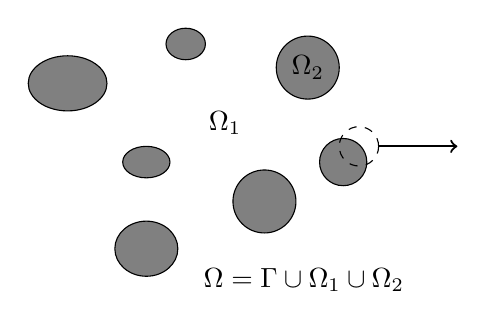
\begin{tikzpicture}
        \foreach \x/\y/\ra/\r in {
        1/3/0.2/0.25,
        2.55/2.7/0.4/0.4,
        0.5/0.4/0.35/0.4,
        2/1/0.4/0.4,
        3/1.5/0.3/0.3,
        0.5/1.5/0.2/0.3,
        -0.5/2.5/0.35/0.5}{
            \draw[fill=gray](\x,\y) ellipse(\r cm and \ra cm);
        }
        \draw[dashed](3.2,1.7)circle(0.25);
        % \draw[thick,->](3.2,1.7)++(0.1767,0.1767)--++(0.4,0.4)--++(1,0);
        \draw[thick,->](3.2,1.7)++(0.25,0)--++(1,0);
        \draw(2.55,2.7)node{$\Omega_2$};
        \draw(1.5,2)node{$\Omega_1$};
        \draw(2.5,0)node{$\Omega = \Gamma \cup \Omega_1 \cup \Omega_2$};
        % \draw(2.5,-1)node{$\Gamma = \sum_\alpha \Gamma_\alpha$};
        % \draw(2.5,-0.5)node{$\Omega_2 = \sum_\alpha \Omega_\alpha$};
    \end{tikzpicture}
    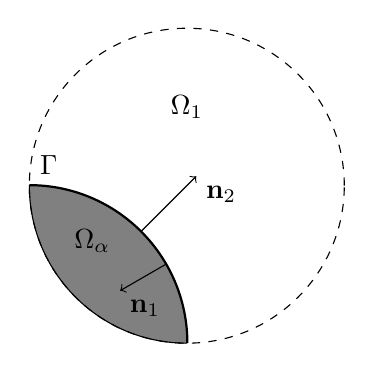
\begin{tikzpicture}%[scale = 0.9]
        \draw[very thick](0:2)arc(0:90:2)node[above right]{$\Gamma$};
        \draw[fill=gray](0:2)arc(0:90:2)arc(180:270:2);
        \draw[dashed](2,2)circle(2);
        \draw[->](1.42,1.42)--++(0.7,0.7)node[below right]{$\textbf{n}_2$};
        \draw[->](1.73,1)--++(-0.577,-0.333)node[below right]{$\textbf{n}_1$};
        \draw(2,3)node{$\Omega_1$};
        \draw(0.8,1.3)node{$\Omega_\alpha$};
    \end{tikzpicture}
    \caption{Domain definitions and scheme of the topology of dispersed two-phase flows.}
    \label{fig:Scheme}
\end{figure}
We consider a system consisting of two phases, separated by a sharp interface $\Gamma(t)$ which evolves over time. 
Each phase subdomain is denoted $\Omega_1(t)$ and $\Omega_2(t)$ for the continuous phase ($1$) and the dispersed phase ($2$) respectively (see \ref{fig:Scheme}). 
The mathematical and physical definition of $\Gamma(t)$ is by no means straightforward, therefore, the interested reader is refereed to \cite{bothe2022sharp} to have a deeper understanding of sharp interface modeling. 
The entire domain, denoted as $\Omega$, is defined as the union of $\Omega_1$, $\Omega_2$, and $\Gamma$.
To track the position of the phase indexed $k$ and the interfaces, we introduce the phase indicator function and the interface indicator function, 
\begin{align}
    \chi_k(\textbf{x},t) =  \left\{
      \begin{tabular}{cc}
        $1 \;\text{if} \;\textbf{x} \in \Omega_k(t)$\\
        $0 \;\text{if} \;\textbf{x} \notin \Omega_k(t)$
      \end{tabular}
      \right.
      \text{for $k = 1,2$},
    %   \label{eq:PIF}
    && \delta_I(\textbf{x},t) =  \left\{
      \begin{tabular}{cc}
        $1 \;\text{if} \;\textbf{x} \in \Gamma(t)$\\
        $0 \;\text{if} \;\textbf{x} \notin \Gamma(t)$
      \end{tabular}
      \right.,
      \label{eq:PIF}
\end{align}
respectively. 
For clarity, we omit the time and position arguments of $\chi_k(\textbf{x},t)$ and $\delta_I(\textbf{x},t)$ in the following sections. 

For the purpose of clarity, we only consider the specific case of the mass, momentum and energy conservation equations for a buoyant dispersed two phase flow.
Equally, we consider a constant density and viscosity in each domain as well as a constant surface tension on the interfaces.

% \subsubsection{Inside the volumes}
Within phase $k$, we note $\rho_k$ the density, $\textbf{u}_k^0$ the local velocity and $E_k^0$ the local total energy per units of mass.
All over the domain $\Omega_k(t)$ the mass, momentum and total energy obey these conservation laws :
\begin{align}
    \label{eq:dt_rho}
    \pddt \rho_k  
    + \div (
        \rho_k\textbf{u}_k^0
    )
    &= 
    0\\
    \label{eq:dt_rhou_k}
    \pddt (\rho_k\textbf{u}_k^0)  
    + \div (
        \rho_k\textbf{u}_k^0\textbf{u}_k^0
        - \bm{\sigma}_k^0 
    )
    &= 
    \rho_k \textbf{g}\\
    \label{eq:dt_rhoE_k}
    \pddt (\rho_kE_k^0)  
    + \div (
        \rho_kE_k^0\textbf{u}_k^0
        + \textbf{q}_k^0
        - \textbf{u}_k^0 \cdot \bm{\sigma}_k^0 
        )
    &= 
    \textbf{u}_k^0 \cdot \textbf{g}  \rho_k
\end{align} 
All along this work the continuous phase will be considered as Newtonian fluid thus, $\bm{\sigma}_1^0 = - p_1^0 \textbf{I} + \bm{\tau}_1^0$ where $\bm{\tau}_1^0$ is the Newtonian stress tensor with $p_1 ^0$ the local pressure and $\bm{\tau}_1^0 = \mu_1[\grad \textbf{u}_1^0+(\grad \textbf{u}_1^0)^T]$ the shear rate. 
The vector $\textbf{q}_k^0$ represent the thermal energy flux and is often model with a Fourier law : $\textbf{q}_k^0 = -\lambda \grad T_k^0$ where $T_k$ is the temperature and $\textbf{g}$ is the acceleration of gravity which will be the only body force in the present problem. 
All along this work the superscript $^0$ indicate that the variable is defied at the local or microscopic scale, in opposition to the averaged or macroscopic quantities that will be presented latter. 

% \subsubsection{On interfaces}

On the interfaces the mass, momentum and total energy balance equations reduce to the common expressions :
\begin{align}
    \label{eq:dt_rho_I}
    \textbf{u}_I = \textbf{u}_k
    &=0, \\
    \Jump{\bm{\sigma}_k^0} 
    &=
    \divI\bm\sigma^0_{I||}
    =
    \gamma\kappa\textbf{n},
    % + \gradI\sigma 
    \label{eq:surface_tension}\\
    \label{eq:dt_rhoI_uI2}
    \Jump{\textbf{u}_k^0 \cdot \bm{\sigma}_k^0}
    &=
     \gamma\kappa\textbf{n}\cdot \textbf{u}_{I}^0\\
    \label{eq:dt_rhoIe_I}
    \Jump{ \textbf{q}_k^0}
    &= 
     0
\end{align}
for the interface kinetic energy and the internal interface energy, respectively. 
Notice that this decomposition is possible only under the assumption of no mass transfer in which case $\textbf{u}_I^0=\textbf{u}_k^0$ for $k =1,2$ and a constant surface tension coefficient.



\section{Lagrangian equations for the dispersed phase}
% \label{sec:Lagrangian}

\subsection{Generic first order description of the particles}

Let us introduce the fundamental Lagrangian properties of a single particle. 
We define the mass, position of the center of mass, momentum, second moment of mass, and moment of momentum, including both the symmetric and skew-symmetric parts, of particle $\alpha$ such as, 
\begin{align}
    m_\alpha
    &= \intO{ \rho_d  },\\
    \textbf{x}_\alpha
    &= \frac{1}{m_\alpha }\intO{ \rho_d \textbf{x} },\\
    \textbf{p}_\alpha 
    &= \intO{ \rho_d \textbf{u}_d^0 },\\
    % & m_\alpha E_\alpha 
    % &= \intO{ \rho_d [e_d^0 + (u_d^0)^2/2] },\\
    \textbf{M}_\alpha 
    &= \intO{ \rho_d \textbf{rr} }, \\
    \textbf{S}_\alpha 
    &= \frac{1}{2}\intO{ \rho_d (\textbf{r}\textbf{u}_d^0+\textbf{u}_d^0\textbf{r}) },\\
    \bm\mu_\alpha 
    &= \intO{ \rho_d \textbf{r}\times\textbf{u}_d^0 },
    \label{eq:position_and_momentum_def}
\end{align}
respectively. 
We recall that $\textbf{r} = \textbf{x} - \textbf{x}_\alpha$ and that $\textbf{u}_\alpha = \textbf{p}_\alpha /m_\alpha$ is the definition of the center of mass velocity in the absence of mass transfer. 
Following the assumptions made in the preceding subsection and the generalized derivation proposed in \ref{chap:daniel2} it can be readily shown that each of these quantities satisfies the following conservation equations:
\begin{align}
    \label{eq:dt_m_alpha}
    \ddt m_\alpha
    &= 
    0\\
    \ddt {\textbf{x}_\alpha}
    &=\textbf{u}_\alpha. 
    \label{eq:dt_x_alpha}\\
    \label{eq:dt_p_alpha}
    \ddt \textbf{p}_\alpha
    &= 
    m_\alpha\textbf{g}
    +  \intS{\bm{\sigma}_f^0 \cdot \textbf{n}_d}\\
    \ddt {\textbf{M}_\alpha}
    &=2\textbf{S}_\alpha. 
    \label{eq:dt_M_alpha}
    \\
    \ddt {\textbf{S}_\alpha}
    &= \intO{ \left(
        \rho_d  \textbf{w}_d^0 \textbf{w}_d^0 
        - \bm{\sigma}_d^0
    \right) }
    - \intS{ 
        \gamma (\bm\delta - \textbf{nn})
    }
    + \frac{1}{2}\intS{ (\textbf{r}\bm{\sigma}_f^0+\bm{\sigma}_f^0\textbf{r})\cdot \textbf{n}_d} 
    \label{eq:dt_S_alpha}\\
    \ddt {\bm\mu_\alpha}
    &=
     \intS{ \textbf{r}\times(\bm{\sigma}_f^0\cdot \textbf{n}_d)} 
    \label{eq:dt_mu_alpha}
    % \label{eq:dt_E_alpha}
    % \ddt E_\alpha^\text{tot}
    % &= 
    % m_\alpha \textbf{u}_\alpha \cdot \textbf{g}
    % +\textbf{u}_\alpha \cdot \intS{\bm{\sigma}_f^0 \cdot \textbf{n}_d}
    % +\intS{\textbf{w}_f^0 \cdot \bm{\sigma}_f^0 \cdot  \textbf{n}_d} 
    % - \intS{\textbf{q}_f^0 \cdot \textbf{n}_d} 
\end{align}
This set of equations can be complemented with an equation for $M_\alpha = \frac{1}{3}\intO{\rho_d \textbf{r}\cdot \textbf{r}}$ which is obtained by taking the double contracted product of\ref{eq:dt_S_alpha} with $\bm\delta$,
it reads, 
\begin{equation}
    \frac{3}{2}\frac{d^2 M_\alpha}{dt^2}
    - \intO{ \rho_d \textbf{w}_d^0 \cdot \textbf{w}_d^0}
    = 
    - \intO{\bm\sigma_d^0:\bm\delta} 
    % - \frac{1}{3}\intS{p_f^0 \textbf{r}\cdot \textbf{n}}
    - \gamma 2 \intS{}
    % - \frac{1}{3}\intS{p_f^0 \textbf{r}\cdot \textbf{n}}
    + \intS{\textbf{r}\cdot\bm\sigma_f^0\cdot \textbf{n}}.
    \label{eq:dt_D_alpha}
\end{equation}
At this stage, the properties and evolution equations of the particles remain general and can be adapted to various types of problems. 
This general framework involves integrals of local quantities, such as $\textbf{w}_d^0$, $\bm\sigma_d^0$ \ldots and others, which are currently unknown. 
Therefore, these integral terms can be considered as closure terms since they are not yet expressed in terms of the Lagrangian unknowns, referred to as the particle's fundamental properties.
For example, in the case of solid particles, we can simplify most of these integral terms by substituting the particle's internal velocity, $\textbf{w}_d^0$ with $ \bm\omega \times \textbf{r}$. 
This solid body motion represents the simplest closure for these equations.  
Thus, for deformable fluid particles, we must find a way to reduce the degrees of freedom related to the particle shape and internal motion and develop a method to simplify the corresponding equations by finding closures for $\bm\sigma_d^0$ and $\textbf{w}_d^0$.
Consequently, in the next section, we adopt restrictive hypotheses regarding the particle shape and internal kinematics, which will allow us to partially close these equations.
% 
\subsection{Spheroidal fluid particles}

Many studies have been conducted to determine the influence of the droplets' deformation on suspension Rheology \citet{goddard1967nonlinear,lhuillier1987phenomenology,maffettone1998equation}.
Most of the authors considered the Rheology of such an emulsion for neutrally buoyant droplets in shearing flow. 
In this work we would to present a first glimps  of the form Rheology of deformable droplets or bubbles with relative motion. 
As a first step to describe the rheology we are interested in the kinematic and dynamic of a single deformable drop. 
In \ref{sec:Exemples} we study the case of 

\subsubsection*{The drop shape}

In this study we consider spheroidal particles described by a conformation tensor that we note $\textbf{C}_\alpha(t)$.  
This tensor is defined such that its eigenvalues are the dimensionless square length of the semi-axis of the spheroid minus one, such that $\textbf{C}_\alpha = (a_1^2/a^2 - 1) \textbf{pp} + (a_2^2 /a^2 - 1) (\textbf{I}-\textbf{pp})$ where $r$ is the radius of the sphere of same volume and \textbf{p} the orientation vector of the particle (see Figure \ref{fig:scheme2}).  
In this way $\textbf{C}_\alpha = 0$ when the particle is spherical and  $\textbf{C}_\alpha + \textbf{I}$ is equivalent to the Cauchy strain tensor well-defined in solid mechanics \citet{mwasame2017macroscopic}. 
In a general coordinate system the point on the surface of the spheroid verify the relation, 
\begin{equation*}
    \textbf{r}\cdot(\textbf{C}_\alpha + \textbf{I})^{-1}\cdot\textbf{r} = a^2,
\end{equation*}
\tb{is it really usefull to define this traceless matrix instead of the actual ellipse}
where $^{-1}$ is the inverse operator.  
One can verify that the second order moment of mass of the particles is related to the conformation tensor through, $\textbf{M}_\alpha = \frac{m_\alpha  a^2}{5} (\textbf{C}_\alpha + \textbf{I})$. 
The last property of the of this tensor is that it the constant volume conservation can be obtained by ensuring that $\text{det}(\textbf{C}_\alpha +\textbf{I}) = (a_1a_2^2)^2 /(a^6) = 1$. 
\begin{figure}[h!]
    \centering
    \hfill
    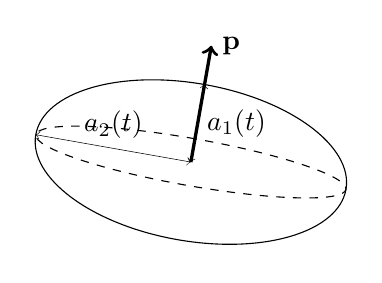
\begin{tikzpicture}[rotate=80]
        \draw(0,0) ellipse (1 cm and 2 cm);
        \draw[dashed](0,0) ellipse (0.3 cm and 2 cm);
        \draw[<->,very thin](0,0) --++ (1,0)node[midway,right]{$a_1(t)$};
        \draw[->,very thick](0,0) --++ (1.5,0)node[right]{$\textbf{p}$};
        \draw[<->,very thin](0,0) --++ (0,2)node[midway,above]{$a_2(t)$};
    \end{tikzpicture}
    \hfill
    \caption{Scheme of an  oblate spheroid oriented along the unit vector \textbf{p} with $a_1(t)$ and $a_2(t)$ the length of the semi axes of the spheroid.}
\end{figure}


\subsubsection*{The droplet internal velocity}

The internal velocity of a solid elastic particle following a homogeneous linear deformation can be described such as $\textbf{w}_2^0 = \bm\Gamma_\alpha \cdot \textbf{r}$ where we have introduced, $\bm\Gamma_\alpha$, the mean velocity gradient inside the particle, which symmetric part : $\textbf{E}_\alpha$, represents the rate of strain, and skew symmetric part : $\bm\Omega_\alpha$, represents the angular velocity. 
Even through the velocity fields $\textbf{w}_2^0 = \bm\Gamma_\alpha \cdot \textbf{r}$  can apply for liquid deforming droplet, an additional flow is present. 
Indeed, from the solution of the stokes equations we can predict the flow within a spherical isolated drop immersed in an unbounded fluid. 
Especially, we know that an solated droplet in translation exhibit internal motion known as Hill vortexes, see \ref{fig:flowlines} (b). 
For a drop immersed in an unbounded linear flow we can also derive an analytical solution such that $\textbf{w}_2^0 \sim \textbf{rrr}$, see \ref{fig:flowlines} (a). 
Therefore, the droplet's internal velocity fields is constituted with a component accounting for the complex internal motions that does not alter the shape of the drop, and another component that account for the linear deformation of the drop.  
\begin{figure*}
    \centering
    \begin{tikzpicture}
        \node (img3) at (0.6\textwidth,0) {\includegraphics[width=0.3\textwidth,angle=270]{image/Rising_def_Stokes.png}};
        \node (img2) at (0.3\textwidth,0) {\includegraphics[width=0.3\textwidth]{image/Rising_Stokes.png}};
        % \draw (0.45\textwidth,0)node{$\rightarrow$};
        % \draw (0.45\textwidth,0.4cm)node{$\bm\Gamma_\alpha\cdot \textbf{r}$};
        \node (img1) at (0.0\textwidth,0) {\includegraphics[width=0.3\textwidth]{image/Shear_Stokes.png}};
        \draw (img3.south)node{(c)};
        \draw (img2.south)node{(b)};
        \draw (img1.south)node{(a)};
    \end{tikzpicture}
    \caption{Three examples of steady state flow lines plots of an isolated droplet immersed into a viscous fluid. 
    (a) Rising sphere in uniform stokes flow (analytical solution in \ref{ap:Translating_sphere}). 
    (b) Fixed droplet in extensional flow (analytical solution in \ref{ap:Translating_sphere}).
    (c) Deformed droplet in rising motion (analytical solution of \citet{taylor1964deformation}). }
\end{figure*}
Consequently, the particle internal velocity might be written, 
\begin{equation}
    \textbf{w}_{2,i}^0(\textbf{x}_\alpha)
    = \bm\Gamma_{\alpha,ik}(t) \cdot \textbf{r}_k
    + \textbf{w}^{s}_{2,i}(t,\textbf{r})
    =\bm{\Omega}_{\alpha,ik}\cdot \textbf{r}_k
    + \textbf{E}_{\alpha,ik} \cdot \textbf{r}_k
    + \textbf{w}^{s}_{2,i}(t,\textbf{r})
\end{equation}
Where we introduced the vector $\textbf{w}^{s}_2(t,\textbf{r}) =\textbf{w}^{0}_{2,i}(t,\textbf{r})  - \bm\Gamma_{\alpha,ik}(t) \cdot \textbf{r}_k$ which represents all the internal motions that does not alter the drop's shape. 
Examples of such motions are displayed \ref{fig:flowlines}. 


From now on we consider that the internal velocity $\textbf{w}^{s}_2(t,\textbf{r})$ is not part of the particles unknown, but a function entirely determined by the particle and flow properties such that $\textbf{w}^{s}_2(t,\textbf{r}) =f_\textbf{w}(\textbf{u}_\alpha,\textbf{C}_\alpha,\bm\Gamma_\alpha,\textbf{u}_1,\bm \Gamma_1,\phi_2) $, where $\bm\Gamma_1 = \grad \textbf{u}_1$ and $\textbf{u}_1$ is the mean velocity fields evaluated at the particle position. 
As it is demonstrated in \ref{ap:Translating_sphere} the internal motion of an isolated spherical drop such as the one in \ref{eq:def_vel} might be determined theoretically from the relative motion and flow fields gradient in the limit of low Reynolds number.
We assume that such a relation exist for other regime. 
Consequently, The particle mean velocity gradient $\bm\Gamma_\alpha$ and its conformation tensor $\textbf C_\alpha$ are the only unknown of our problem. 
Therefore, we need to provide two equations, one for $\textbf{C}_\alpha$ and another for $\bm\Gamma_\alpha$. 

\subsubsection*{Kinematic and dynamic of a deformable spheroid}

The evolution of $\textbf{C}_\alpha$ and $\bm\Gamma_\alpha$ will be described by the second moment of mass and first moment of momentum equation.
Consequently, we must reformulate the terms in \ref{eq:dt_M_alpha} and \ref{eq:dt_P_alpha} in terms of $\textbf{C}_\alpha$ and $\bm\Gamma_\alpha$. 
The integrals constitutive of these moments equations can be written, 
\begin{align}
    \intO{(\textbf{rw}_2^0 )_{ij}+ (\textbf{w}_2^0 \textbf{r})_{ij}} 
    = \textbf{C}_{\alpha,ik} \cdot \bm\Gamma_{\alpha,kj}
    +  \bm\Gamma_{\alpha,ki} \cdot \textbf{C}_{\alpha,jk}
    +  \bm\Gamma_{\alpha,ij} + \bm\Gamma_{\alpha,ij}
    \\
    \intO{\rho_2 \textbf{w}_{2,i}^0\textbf{w}_{2,j}^0}
    = \frac{m_\alpha a^2}{5}[
        \bm\Gamma_{\alpha,lj}\bm\Gamma_{\alpha,ki} \textbf{C}_{\alpha,kl} 
        + \bm\Gamma_{\alpha,kj}\bm\Gamma_{\alpha,ki} 
        % + f_\textbf{ww}(\textbf{u}_\alpha,\textbf{C}_\alpha,\bm\Gamma_\alpha,\textbf{u}_1,\bm \Gamma_1,\phi_2)
        + f_\textbf{ww}(\textbf{u}_\alpha,\textbf{C}_\alpha,\bm\Gamma_\alpha,\textbf{u}_1,\bm \Gamma_1,\phi_2)
        ]
    \\
    \intO{\bm\sigma_{2,ij}^0}
    =
    % -\intO{p_2^0} \textbf{I}_{ij}
    \mu_2 v_\alpha [\bm\Gamma_{\alpha,ij} + \bm\Gamma_{\alpha,ij}
    + f_{\bm{\sigma}}(\textbf{u}_\alpha,\textbf{C}_\alpha,\bm\Gamma_\alpha,\textbf{u}_1,\bm \Gamma_1,\phi_2)]
    % + \textbf{I}_{ij}\intO{p_2^0} 
    \\
    \intS{\bm\sigma_{I,ij}^0}
    = \frac{2 \gamma v_\alpha }{a} \textbf{I}_{ij} - \frac{4 \gamma v_\alpha }{5 a} \textbf{C}_{\alpha,ij}
    +\mathcal(|\textbf{C}|^2)\\
    \intS{\textbf{r}\bm\sigma_1^0\cdot \textbf{n}_2}
    = 
    \frac{1}{2}\intS{(\textbf{r}\bm\sigma_1^0-\bm\sigma_1^0\textbf{r})\cdot \textbf{n}_2}
    + \frac{1}{2}\intS{(\textbf{r}\bm\sigma_1^0+\bm\sigma_1^0\textbf{r})\cdot \textbf{n}_2}
    % \textbf{M}(\textbf{u}_\alpha,\textbf{C}_\alpha,\bm\Gamma_\alpha,\textbf{u}_1,\bm \Gamma_1,\phi_2)
\end{align}
\tb{carry the actual decomposition with the velocity components }
\tb{mettre sous forme plus simple et expliquer l'osciallater sous forme 1d}
First, as discussed above only the deforming motion contribute to the symmetric part of the moment of momentum, we could therefore express it explicitly in terms of the particle unknown. 
Regarding the first moment of the surface tension, it has been computed analytically carrying a surface integral on the ellipsoidal surface of the droplet. 
Since, the droplets remain spheroidal under small deformation we choose to approximate $\intS{\bm\sigma_I^0}$ with its first order Taylor series in $\textbf{C}_\alpha$ without lost of generality.
Note that our expression of $\intS{\bm\sigma_I^0}$ is in agreement with \citet{lhuillier1987phenomenology} if one account for the slight difference of his definition of the deformation tensor which is half of $\textbf{C}_{\alpha}$. 
% in which our $\textbf{C}_\alpha$ is twice his, in the limit of small \textbf{C}_\alpha.
For the expression of $\intO{\rho_2 \textbf{w}_{2,i}^0\textbf{w}_{2,j}^0}$, $ \intO{\bm\sigma_{2,ij}^0}$ we had to introduce two unknown functions, $f_\textbf{ww}$, $f_{\bm{\sigma}}$, which vanish when $\textbf{w}^s_2 =0$. 
Therefore, these expressions are a sum of a function involving $\bm\Gamma_\alpha$ and an unknown part which depend on the parameters of the problem and need to be closed. 
The expression of $\intO{\rho_2 \textbf{w}_{2,i}^0\textbf{w}_{2,j}^0}$, $ \intO{\bm\sigma_{2,ij}^0}$ and $\intS{\textbf{r}\bm\sigma_1^0\cdot \textbf{n}_2}$ are very problem dependent. 
To provide a clearer example we computed these terms in \ref{ap:Translating_sphere} in the simplified scenario of an isolated droplet in a general linear flow. 

% The most common example is the expression for first moment \textbf{M}, which has been widely investigated in the pure straining situation, an example is given in \ref{ap:Translating_sphere} for spherical drop, and in \citet{raja2010inertial} for slightly deformable droplet in inertial flows. 
% It is important to notice that these functions are dependent of the relative drop-carrier fluid velocity, in such a way that the momentum and first moment of momentum are linked through the function $f_{\textbf{ww}},f_{\bm{\sigma}}$ and $\intS{\textbf{r}\bm\sigma_1^0\cdot \textbf{n}_2}$. 
% Indeed, even if it has been uniquely studied in pure linear flows, the relative motion of a particle might generate a first moment on its surface. 


At this point it wouldn't be wise trying to find an expression for each of these unknown functions in such a generality. 
Instead, we expose the unclosed set of equation of motions for spheroidal particles. 
In addition to the previously exposed equations (mass, momentum and energy equation) this system is constituted of three equations, one for $\textbf{C}_\alpha$ and two equation for the moment of momentum, the symmetric and skew-symmetric moment of momentum. 
% These read, 
\begin{align*}
    \ddt \textbf{C}_{\alpha,ij}
    = \textbf{C}_{\alpha,ik} \cdot \bm\Gamma_{\alpha,kj}
    +  \bm\Gamma_{\alpha,ki} \cdot \textbf{C}_{\alpha,jk},\\
    \frac{a^2  m_\alpha}{5} \ddt( \textbf{C}_{ik} \cdot \bm\Gamma_{\alpha,kj}
    -  \bm\Gamma_{\alpha,ki} \cdot \textbf{C}_{jk})
    =  \intS{(\textbf{r}\bm\sigma_2^0- \bm\sigma_2^0\textbf{r})\cdot \textbf{n}}\\
    \frac{m_\alpha a^2}{5}\ddt^2 \textbf{C}_\alpha
    - \frac{m_\alpha a^2}{5}[
    \bm\Gamma_{\alpha,lj}\bm\Gamma_{\alpha,ki} \textbf{C}_{\alpha,kl} + f_\textbf{ww}]
    + \mu_2 v_\alpha [(\bm \Gamma_{p,ij}+\bm \Gamma_{p,ji})
    + f_{\bm{\sigma}}]\\
    + \frac{2 \gamma v_\alpha }{a} \textbf{I}_{ij} 
    - \frac{4 \gamma v_\alpha }{5 a} (\textbf{C}_{ij} - \textbf{I}_{ij})
    = \intS{(\textbf{r}\bm\sigma_2^0+ \bm\sigma_2^0\textbf{r})\cdot \textbf{n}}
    % + \textbf{I}_{ij}\intO{p_2^0}
\end{align*}
% Where we placed the unknown function at the right hands side of these equations. 
Now, we would like to propose a more intuitive interpretation of the mass and momentum equations.
To that end, we make the problem dimensionless by introducing, 
the \textit{Capillary number} $Ca= \frac{\mu_1 U}{\gamma}$, The viscosity ratio $\lambda = \mu_2/\mu_1$, the density ratio $\zeta = \rho_2/\rho_1$ and the Reynolds number $Re = \frac{a U \rho_1}{\mu_1}$, with $U$ as the velocity scale. 
%  such that  $\bm\Gamma_\alpha'  = \frac{a}{U}\bm\Gamma$, and $\tau_a$ the timescale related to the drop shape evolution.
In the low Reynolds regime the first moment of surface traction forces will be proportional to a viscous stress (see \ref{ap:Translating_sphere}), therefore :$\intS{\textbf{r}\bm\sigma_2^0\cdot \textbf{n}} =\mu_1  \tau v_\alpha \intS{\textbf{r}\bm\sigma_2^0\cdot \textbf{n}}^*$, with $\tau$ the inverse timescale of the external solicitation.
The ratio between the external flow scale $\tau$ and the drop timescale $\tau_a$ is noted $\beta$. 
With that in mind, \ref{eq:dt_M_alpha}, \ref{eq:dt_mu_alpha} and \ref{eq:dt_S_alpha} might be written :
\begin{align}
    \beta \ddt \textbf{C}_{\alpha,ij}
    - \textbf{C}_{\alpha,ik} \cdot \bm\Gamma_{\alpha,kj}^*
    - \bm\Gamma_{\alpha,ki}^* \cdot \textbf{C}_{\alpha,jk},
    = 
    \bm\Gamma_{\alpha,ij}^*
    +  \bm\Gamma_{\alpha,ji}^*\\
    Re \zeta \beta \ddt( \textbf{C}_{\alpha,ik} \cdot \bm\Gamma_{\alpha,kj}^*
    -  \bm\Gamma_{\alpha,ki}^* \cdot \textbf{C}_{\alpha,jk}
    + \bm\Gamma_{\alpha,ji} - \bm\Gamma_{\alpha,ij})
    =  \intS{(\textbf{r}\bm\sigma_2^0- \bm\sigma_2^0\textbf{r})\cdot \textbf{n}}^*\\
    \zeta Re \frac{1}{5}  
    \left[
        \frac{1}{2}\beta^2 \ddt^2_* \textbf{C}_\alpha
        - \bm\Gamma_{\alpha,lj}^* \bm\Gamma_{\alpha,ki}^* \textbf{C}_{\alpha,kl}^* 
        - \bm\Gamma_{\alpha,kj}^* \bm\Gamma_{\alpha,ki}^* 
        - f_\textbf{ww}
    \right]\nonumber\\
    + \lambda \left[
        \beta \ddt \textbf{C}_{\alpha,ij}
        -\textbf{C}_{\alpha,ik} \cdot \bm\Gamma_{\alpha,kj}
        - \bm\Gamma_{\alpha,ki}^* \cdot \textbf{C}_{\alpha,jk},
        + f_{\bm{\sigma}}
    \right]\nonumber\\
    - \frac{1}{Ca}\left[
        \frac{4}{5} \textbf{C}_{\alpha,ij}
        +2 \textbf{I}_{ij} 
    \right]
    =
    \frac{1}{2}\intS{(\textbf{r}\bm\sigma_1^0+ \bm\sigma_1^0\textbf{r})\cdot \textbf{n}}^*
\end{align}
\tb{at this point it is not usefull to introduce the substitution in the last equaiton instead explain that it is proportional to the derivative in the limit}
The second moment of mass \ref{eq:dt_Cs}, is consistent with the equation found by \citet{goddard1967nonlinear} and \citet{lhuillier1987phenomenology}. 
Following, \citet{goddard1967nonlinear}  terminology, the left-hand side of \ref{eq:dt_Cs} is referred as the \textit{convected} derivative of $\textbf{C}^*_\alpha$. 
Therefore, the \textit{convected} derivative of $\textbf{C}_\alpha$ is equal to the rate of strain of the particle. 
The skew-symmetric part of the first moment of momentum \ref{eq:dt2_C}, it is basically the angular momentum balance of a non-spherical object. 
The right-hands side accounting for the external torque contribution. 
The symmetric part however has the form of a non-linear forced harmonic oscillatory equation for the droplet deformation. 
Indeed, the first groups of terms on the left-hand side represent the inertial contribution of the droplet internal fluid. 
It is made of a second order derivative plus non-linear terms in $\bm\Gamma_\alpha$. 
The second groups of terms is internal viscous contribution that arise directly from the definition of the stress \ref{eq:sigma_2_def}. 
It vanishes for small viscosity ration and is linear in the first derivative of $\textbf{C}_\alpha$. 
The last term on the left-hand side is the elastic response from the interface which is negligible for high capillary number $Ca \to \infty$. 
Then on right-hand side of the equation we find the first moment of surface force, $\intS{(\textbf{r}\bm\sigma_1^0+ \bm\sigma_1^0\textbf{r})\cdot \textbf{n}}^*$ which has an unknown expression at this stage. 
\ref{eq:dt2_C} might be regarded as a second order harmonic equation with non-linear contributions. 
However, the unknown function $f_\textbf{ww},\ f_{\bm{\sigma}}$ and $\intS{(\textbf{r}\bm\sigma_1^0+ \bm\sigma_1^0\textbf{r})\cdot \textbf{n}}^*$ are in general function of $\textbf{C}_\alpha$ and its higher derivatives of $\textbf{C}_\alpha$.   
Therefore, at this stage it is impossible to predict the nature of the harmonic regime followed by the droplet. 
To conclude on this matter one must find an expression for all this closure as well as determinate the impact of the non-linear terms.

We now examine the specific case studied by \citet{lamb1924hydrodynamics} where he considered no external contribution around the particle, therefore, $\intS{(\textbf{r}\bm\sigma_1^0+ \bm\sigma_1^0\textbf{r})\cdot \textbf{n}}^* = 0$.
It is found, that the amplitude of the second order harmonic mode of deformation, noted $\epsilon_2$, follows the second order partial differential equations,  
\begin{equation*}
    \ddt^2{\epsilon_2}
    + 2\lambda_2 \ddt \epsilon_2
    + \omega_2^2 \epsilon_2
     = 0,
\end{equation*}
where $\lambda_2$ and $\omega_2$ are the damping and frequency of coefficient defined as, 
\begin{align*}
    \lambda_2 = 5 \frac{\mu_2}{\rho_2a^2},
    && \omega_2 = \sqrt{8 \frac{\mu_2}{\rho_2 a^2}}.
\end{align*}
Where this equation has been obtained in the linear deformation regime for $\epsilon_2 \ll 1$. 
When multiplying \ref{eq:dt2_C} by, $\frac{10}{\zeta Re}$ we indeed find the exact same coefficient $\lambda_2$ and $\omega_2^2$ in front of, $\ddt \textbf{C}_{\alpha,ij}$ and $\textbf{C}_{\alpha,ij}$, respectively. 
In the limit of small $\textbf{C}_\alpha$, only these linear terms remain, therefore consistent with the reference work of \citet{lamb1924hydrodynamics}. 
\ref{eq:dt2_C} is somewhat more general than lamb's solution since it is expressed in an arbitrary reference frame. 
Which will prove to be useful in \ref{sec:Exemples} were we apply ensemble average on these quantities. 
However, with this equation we are able to describe only the second oscillatory mode. 
To study higher order modes one must use higher moment of momentum equations. 

In the past studies, the coupling between translational and oscillating nature of rising bubbles or droplets have been investigated \citet{lalanne2013effect}. 
For an isolated spherical droplet in translation through a stokes or potential flow we know that $
    f_\textbf{ww}
    = \frac{m_\alpha}{140 (\lambda +1)^2}
    (7 \textbf{u}_{\alpha 1} \textbf{u}_{\alpha 1} + \textbf{u}_{\alpha 1}\cdot \textbf{u}_{\alpha 1}\textbf{I})$, 
(see \ref{ap:Translating_sphere}). 
It is reasonable to guess that for a slightly spheroidal droplet in translation the expression might preserve the same form. 
Indeed, a coefficient related to $\textbf{C}_\alpha$ might appear in the expression nevertheless the overall contribution must be still proportional to $\textbf{u}_{\alpha 1} \textbf{u}_{\alpha 1}$. 
Likewise, for an inertial drops, it might be found that 
$\intS{(\textbf{r}\bm\sigma_1^0+ \bm\sigma_1^0\textbf{r})\cdot \textbf{n}}^* \sim A \textbf{u}_{\alpha 1} \textbf{u}_{\alpha 1} + B \textbf{u}_{\alpha 1} \cdot \textbf{u}_{\alpha 1}$ where $A$ and $B$ are constant. 
Indeed, the translational motion a spherical particle at slight inertia induce an overall unbalance stress on the surface of the particle generating a first moment \citet{taylor1964deformation}. 
The point is that the yet unknown closures, will help us bridge translational and drop's straining motions. 
Therefore, injecting these expressions into \ref{eq:dt2_C} would be a first step to accomplish a coupling between oscillating, or deforming motion with translating motion.
This is the subject of the last section. 
Obviously, now that we obtained a general formulation for the dynamic of the droplets' deformation, the most challenging aspect is to find expressions for closure terms. 


\subsubsection*{The particle internal energy balance.}

The surface of the particles, and internal kinetic energy can be written in this context as, 
\begin{align*}
    \beta \ddt \textbf{C}_{\alpha,ij}
    - \textbf{C}_{\alpha,ik} \cdot \bm\Gamma_{\alpha,kj}^*
    - \bm\Gamma_{\alpha,ki}^* \cdot \textbf{C}_{\alpha,jk},
    = 
    2\textbf{E}_{\alpha,ij}\\
    \intO{\rho_2 \textbf{w}_{2,i}^0\textbf{w}_{2,i}^0}
    = \frac{m_\alpha a^2}{5}[
        \bm\Gamma_{\alpha,li}\bm\Gamma_{\alpha,ki} \textbf{C}_{\alpha,kl} 
        + \bm\Gamma_{\alpha,ki}\bm\Gamma_{\alpha,ki} 
        + f_\textbf{ww}(\textbf{u}_\alpha,\textbf{C}_\alpha,\bm\Gamma_\alpha,\textbf{u}_1,\bm \Gamma_1,\phi_2)
        ]
    \\
    \intO{\bm\sigma_{2,ij}^0:\grad \textbf{u}_2^0}
    = 2 \mu_2 \intO{\textbf{e}_2^0:\textbf{e}_2^0}
    = 2\mu_2v_\alpha\left[ \textbf{E}_{\alpha,ij}\textbf{E}_{\alpha,ij}
    + f_{\textbf{e}}\right]\\
    % -\intO{p_2^0} \textbf{I}_{ij}
    \mu_2 v_\alpha [\textbf{E}_{\alpha,ij}
    + f_{\bm{\sigma}}(\textbf{u}_\alpha,\textbf{C}_\alpha,\bm\Gamma_\alpha,\textbf{u}_1,\bm \Gamma_1,\phi_2)]
    % + \textbf{I}_{ij}\intO{p_2^0} 
    \\
    s_\alpha \gamma
    = 
    \frac{3 \gamma v_\alpha }{a}\left[
        1
        + \frac{1}{20}\textbf{C}_\alpha:\textbf{C}_\alpha
    \right]
\end{align*}

\begin{equation}
    \ddt (W_\alpha + \gamma s_\alpha)
    + \intO{ \bm{\sigma}_2^0 : \grad\textbf{u}_2^0 }
    =\intS{\textbf{w}_1^0 \cdot \bm{\sigma}_1^0 \cdot \textbf{n}_2} 
\end{equation}

In conclusion, we have demonstrated how the first and second moment of momentum and mass equation can be used to describe the second mode oscillatory motion of a spheroidal drop in a Galilean reference frame. 
Therefore, the moment of momentum is a quantity of utmost importance for all kinds of particles with variable shape or volume.
This isn't limited to the momentum distribution, but all kind of properties can be described that way. 
In fact, if one wish to describe the first moment of the distribution of any local quantity $f_2^0$ and $f_I^0$ over the surface or volume of the particle, he must use the first moments' conservation equations. 
As an example, the mean concentration and distribution of surfactants on the bubbles' surface have a significant impact on the mass transfer rate between the dispersed and continuous phases.
In this case first moment of surfactant concentration could be considered here to track the evolution of the surfactant concentration and orientation over the particle surface, which would enable us to compute a better approximation of the drag force coefficient. 

% 
% \section{Re-derivation but more easy}
% \label{ap:local_basis_eq}

% All these went way to complicated. 
% So here is a more consize derivation that does keep track of the physics. 
% We describe the geometry of the particle with the second moment of mass tensor, 
% \begin{equation*}
%     M_{\alpha,ij} 
%     =\frac{m_\alpha a^2}{5} M_{\alpha,ij}^*
%     = \frac{m_\alpha a^2}{5}\left[
%         \left(
%             \frac{a_1}{a}
%         \right)^2 p_i p_j
%         + 
%         \left(
%             \frac{a_1}{a}
%         \right)^2(\delta_{ij}-  p_i p_j)
%     \right]
% \end{equation*}
% This tensor has several notable properties, the volume conservation : $a_1 a_2^2 = a^3$ which means that $\textbf{M}_\alpha^*$ has two eigenvalues linked through $M^1 = (M^2)^{-2}$ or $M^2 = (M^1)^(-1/2)$. 
% At small deformation, i.e. $M_1 - 1\ll 1$ we therefore have $M^1 = 1 - (M^1-1)/2$.
% This ultimately means that at small deformation the trace is a constant namely $M_{ij} \delta_{ij} = 3+\mathcal{O}((M^1 -1)^2)$. 




% Let's now reformulate the integral of the problem namely, 
% \begin{align}
%     \intO{(\textbf{rw}_ 2^0 )_{ij}+ (\textbf{w}_2^0 \textbf{r})_{ij}} 
%     = \textbf{M}_{\alpha,ik} \cdot \bm\Gamma_{\alpha,jk}
%         +  \bm\Gamma_{\alpha,ik} \cdot \textbf{M}_{\alpha,jk}
%     \\
%     \intO{\rho_2 \textbf{w}_{2,i}^0\textbf{w}_{2,j}^0}
%     = \bm\Gamma_{\alpha,jl}\bm\Gamma_{\alpha,ik} \textbf{M}_{\alpha,kl}  
%         +\intO{\rho_2 \textbf{w}_{2,i}^s\textbf{w}_{2,j}^s}
%     \\
%     \intO{\bm\sigma_{2,ij}^0}
%     =
%     2 \mu_2 v_\alpha \textbf{E}_{\alpha,ij}
%     - \intO{p_2^0} \textbf{I}_{ij}
%     + \mu_2 \intS{(\textbf{n}_i \textbf{w}_{2,j}^s + \textbf{n}_j \textbf{w}_{2,i}^s)}
%     \\
%     \intS{\bm\sigma_{I,ij}^0}
%     = \frac{\gamma v_\alpha }{a} \left[
%         2\textbf{I}_{ij} 
%         - \frac{4  }{5} (\textbf{M}_{\alpha,ij}^* - \textbf{I}_{\alpha,ij})
%     \right]
%     +\mathcal(O)(\textbf{C}\cdot \textbf{C})\\
%     s_\alpha 
%     = 4\pi a^2 (1+\frac{\textbf{C}:\textbf{C}}{15})
% \end{align}
% for the surface tension term is made of two terms, one corresponding to Laplace pressure and the other to the deviatoric stress. 




% The equation for the orientation, second moment of mass torque, symmetric moment of momentum and trace of the moment of momentum reads, 
% \begin{align*}
%     \ddt \textbf{pp}_{\alpha,ij}
%     = \textbf{pp}_{\alpha,ik} \cdot \bm\Omega_{\alpha,jk}
%     +  \bm\Omega_{\alpha,ik} \cdot \textbf{pp}_{\alpha,jk}\\
%     \ddt \textbf{M}_{\alpha,ij}
%     = \textbf{M}_{\alpha,ik} \cdot \bm\Gamma_{\alpha,jk}
%     +  \bm\Gamma_{\alpha,ik} \cdot \textbf{M}_{\alpha,jk}\\
%     \ddt (\textbf{I}_{\alpha,ik}\bm\omega_{\alpha,k} )
%     = 
%     \intS{(\textbf{r}\times\bm\sigma_1^0\cdot \textbf{n})_i} \\
%     \frac{1}{2}\ddt^2 \textbf{M}_{\alpha,ij}
%     -  \bm\Gamma_{\alpha,jl}\bm\Gamma_{\alpha,ik} \textbf{M}_{\alpha,kl}  
%     + 2 \mu_2 v_\alpha \textbf{E}_{\alpha,ij}
%     + \frac{\gamma v_\alpha }{a} \left[
%     2\textbf{I}_{ij} 
%     - \frac{4 \gamma v_\alpha }{5 a} (\textbf{M}_{\alpha,ij}^* - \textbf{I}_{\alpha,ij})
%     \right]\\
%     = 
%     \frac{1}{2}\intS{(\textbf{r}\bm\sigma_1^0 + \bm\sigma_1^0\textbf{r})\cdot \textbf{n}} 
%     + \intO{\rho_2 \textbf{w}_{2,i}^s\textbf{w}_{2,j}^s}
%     + \intO{p_2^0} \textbf{I}_{ij}
%     - \mu_2 \intS{(\textbf{n}_i \textbf{w}_{2,j}^s + \textbf{n}_j \textbf{w}_{2,i}^s)}\\
%     % \frac{1}{2}\ddt^2 \textbf{M}_{\alpha,mm}
%     -  \bm\Gamma_{\alpha,ml}\bm\Gamma_{\alpha,mk} \textbf{M}_{\alpha,kl}  
%     + \frac{\gamma v_\alpha }{a} 
%     % \left[
%     2\textbf{I}_{mm} 
%     % - \frac{4 }{5 } (\textbf{M}_{\alpha,mm}^* - \textbf{I}_{\alpha,mm})
%     % \right]
%     % \\
%     = 
%     \intS{\textbf{r}_m\cdot\bm\sigma_{1,mk}^0\cdot \textbf{n}_k} 
%     + \intO{\rho_2 \textbf{w}_{2,m}^s\cdot \textbf{w}_{2,m}^s}
%     + \intO{p_2^0} \textbf{I}_{mm}
% \end{align*}

% As the derivative of $M_{ij}$ in these equations actually takes in account the change of orientation of the particle it might be useful to re-derive these equations in the eigenbasis of the matrix $M_{ij}$

% To the first order in deformation the deviatoric part reads, 
% \begin{align*}
%     \frac{1}{2}\ddt^2 \textbf{M}_{\alpha,ij}
%     -   \textbf{M}_{\alpha,kl} 
%     (\bm\Gamma_{\alpha,jl}\bm\Gamma_{\alpha,ik}  
%     - \frac{1}{3}
%     \bm\Gamma_{\alpha,ml}\bm\Gamma_{\alpha,mk}  
%     \textbf{I}_{ij}
%     )
%     + 2 \mu_2 v_\alpha \textbf{E}_{\alpha,ij}
%     - \frac{\gamma v_\alpha }{a} 
%     \frac{4  }{5} (\textbf{M}_{\alpha,ij}- \textbf{I}_{ij})
%     \\
%     = 
%     \frac{1}{2}\intS{(\textbf{r}\bm\sigma_1^0 + \bm\sigma_1^0\textbf{r} - \frac{2}{3}\textbf{r}\cdot \bm\sigma_1^0 \textbf{I})\cdot \textbf{n}} 
%     + \intO{\rho_2 (\textbf{w}_{2,i}^s\textbf{w}_{2,j}^s - \frac{1}{3}\textbf{w}_{2,m}^s\textbf{w}_{2,m}^s \textbf{I}_{ij}) }
%     - \mu_2 \intS{(\textbf{n}_i \textbf{w}_{2,j}^s + \textbf{n}_j \textbf{w}_{2,i}^s)}\\
% \end{align*}
% It can be somewhat useful to extract the proportionality coefficient of each terms. 
% Denotining dimensionless qte by a $*$ we have, 
% \begin{align*}
%     \frac{\rho_2 a^2}{5 \tau^2}\left[\frac{1}{2}\ddt^2 \textbf{M}_{\alpha,ij}^*
%     -  \bm\Gamma_{\alpha,jl}^*\bm\Gamma_{\alpha,ik}^* \textbf{M}_{\alpha,kl}^*
%     \right]  
%     + \frac{2 \mu_2  }{\tau} \textbf{E}_{\alpha,ij}^*
%     + \frac{\gamma  }{a} \left[
%     2\textbf{I}_{ij} 
%     - \frac{4 }{5} (\textbf{M}_{\alpha,ij}^* - \textbf{I}_{\alpha,ij})
%     \right]\\
%     = 
%     \frac{1}{2}\intS{(\textbf{r}\bm\sigma_1^0 + \bm\sigma_1^0\textbf{r})\cdot \textbf{n}} 
%     + \intO{\rho_2 \textbf{w}_{2,i}^s\textbf{w}_{2,j}^s}
%     + \intO{p_2^0} \textbf{I}_{ij}
%     - \mu_2 \intS{(\textbf{n}_i \textbf{w}_{2,j}^s + \textbf{n}_j \textbf{w}_{2,i}^s)}\\
% \end{align*}

% The forcing terms are really problem dependent. 
% Thus, at this stage it cannot be scaled in terms of timescale. 

% In order to be more consis, we may write :
% \begin{align*}
%     \textbf{F}_{ij}(\textbf{w}^s,\bm\sigma_1^0)
%     = 
%     \frac{1}{2}\intS{(\textbf{r}\bm\sigma_1^0 + \bm\sigma_1^0\textbf{r} - \frac{2}{3}\textbf{r}\cdot \bm\sigma_1^0 \textbf{I})\cdot \textbf{n}} 
%     + \intO{\rho_2 (\textbf{w}_{2,i}^s\textbf{w}_{2,j}^s - \frac{1}{3}\textbf{w}_{2,m}^s\textbf{w}_{2,m}^s \textbf{I}_{ij}) }
%     - \mu_2 \intS{(\textbf{n}_i \textbf{w}_{2,j}^s + \textbf{n}_j \textbf{w}_{2,i}^s)}\\
% \end{align*} 
% Indicating that the forcing term is related to the exterior contribution and the external stresses. 

% \begin{align*}
%     \ddt^2 \textbf{M}_{\alpha,ij}^*
%     -2  \textbf{M}_{\alpha,kl}^* 
%     (\bm\Gamma_{\alpha,jl}^*\bm\Gamma_{\alpha,ik}^*  
%     - \frac{1}{3}
%     \bm\Gamma_{\alpha,ml}^*\bm\Gamma_{\alpha,mk}^*  
%     \textbf{I}_{ij}
%     )
%     + \frac{10 \mu_2 \tau}{ \rho_2 a^2} 2\textbf{E}_{\alpha,ij}^*
%     - 8 \frac{\tau^2 \gamma  }{\rho_2 a^3} 
%      (\textbf{M}_{\alpha,ij}^*- \textbf{I}_{ij})\\
%     = 
%     \frac{\tau^2 10}{a^2 m_\alpha}
%     \left[\textbf{F}_{\sigma_1, ij}
%     + \textbf{F}_{ww, ij}
%     + \textbf{F}_{\sigma_2, ij}\right]
% \end{align*}

% All these unclose term are really problem dependent, for now all we now is that at low Reynolds number we are in the viscous regime, besides this external flow that drives these scales. 
% Meaning that, 
% \begin{align*}
%     \intO{\rho_2 \textbf{w}_{2,i}^0\textbf{w}_{2,j}^0}
%     \sim \frac{m_\alpha a^2}{\tau_u^2} \textbf{F}_{ww}^*
%     \\
%     \mu_2 \intS{(\textbf{n}_i \textbf{w}_{2,j}^s + \textbf{n}_j \textbf{w}_{2,i}^s)}
%     \sim \frac{v_\alpha \mu_2}{\tau_u} \textbf{F}_{e}^*
%     \\
%     \intS{\bm\sigma_1^0 \textbf{rn}}
%     \sim 
%     \frac{v_\alpha \mu_1}{\tau_u} \textbf{F}_{\sigma}^*
% \end{align*} 

% \begin{align*}
%     \ddt^2 \textbf{M}_{\alpha,ij}^*
%     -2  \textbf{M}_{\alpha,kl}^* 
%     (\bm\Gamma_{\alpha,jl}^*\bm\Gamma_{\alpha,ik}^*  
%     - \frac{1}{3}
%     \bm\Gamma_{\alpha,ml}^*\bm\Gamma_{\alpha,mk}^*  
%     \textbf{I}_{ij}
%     )
%     + \frac{10 \mu_2 \tau}{ \rho_2 a^2} 2\textbf{E}_{\alpha,ij}^*
%     - 8 \frac{\tau^2 \gamma  }{\rho_2 a^3} 
%      (\textbf{M}_{\alpha,ij}^*- \textbf{I}_{ij})\\
%     = 
%     \frac{\tau^2 10 \mu_1 }{a^2 \rho_2 \tau_u}
%     \textbf{F}_{\sigma_1, ij}
%     + \frac{\tau^2 10}{\tau_u^2} \textbf{F}_{ww, ij}
%     + \frac{\tau^2 10 \mu_1 }{a^2 \rho_2 \tau_u} \textbf{F}_{\sigma_2, ij}
% \end{align*}


% \subsubsection*{Re-derivation but with dimensionless scaling}

% \begin{align}
%     \intO{(\textbf{rw}_ 2^0 )_{ij}+ (\textbf{w}_2^0 \textbf{r})_{ij}} 
%     = \textbf{M}_{\alpha,ik} \cdot \bm\Gamma_{\alpha,jk}
%         +  \bm\Gamma_{\alpha,ik} \cdot \textbf{M}_{\alpha,jk}
%     \\
%     \intO{\rho_2 \textbf{w}_{2,i}^0\textbf{w}_{2,j}^0}
%     = \bm\Gamma_{\alpha,jl}\bm\Gamma_{\alpha,ik} \textbf{M}_{\alpha,kl}  
%         +\intO{\rho_2 \textbf{w}_{2,i}^s\textbf{w}_{2,j}^s}
%     \\
%     \intO{\bm\sigma_{2,ij}^0}
%     =
%     2 \mu_2 v_\alpha \textbf{E}_{\alpha,ij}
%     - \intO{p_2^0} \textbf{I}_{ij}
%     + \mu_2 \intS{(\textbf{n}_i \textbf{w}_{2,j}^s + \textbf{n}_j \textbf{w}_{2,i}^s)}
%     \\
%     \intS{\bm\sigma_{I,ij}^0}
%     = \frac{\gamma v_\alpha }{a} \left[
%         2\textbf{I}_{ij} 
%         - \frac{4  }{5} (\textbf{M}_{\alpha,ij}^* - \textbf{I}_{\alpha,ij})
%     \right]
%     +\mathcal(O)(\textbf{C}\cdot \textbf{C})\\
%     s_\alpha 
%     = 4\pi a^2 (1+\frac{\textbf{C}:\textbf{C}}{15})
% \end{align}

% Then, 
% \begin{align*}
%     \frac{\rho_2 a^2}{5}\left[
%         \frac{1}{\tau^2}\frac{1}{2}\ddt^2 \textbf{M}_{\alpha,ij}
%     -   \frac{1}{\tau^2}\bm\Gamma_{\alpha,jl}\bm\Gamma_{\alpha,ik} \textbf{M}_{\alpha,kl}  
%     - \frac{1}{\tau_u^2} \textbf{F}_{ww}^*
%     \right]\\
%     + \mu_2  \left[
%         \frac{1}{\tau} 2\textbf{E}_{\alpha,ij}
%     + \frac{1}{\tau_u} \textbf{F}_\sigma^*
%     \right]\\
%     + \frac{\gamma  }{a} \left[
%     2\textbf{I}_{ij} 
%     - \frac{4  }{5} (\textbf{M}_{\alpha,ij}^* - \textbf{I}_{\alpha,ij})
%     \right]\\
%     = 
%     \frac{1}{2}
%     \frac{ \mu_1}{\tau_u} 
%     \textbf{F}_{\sigma_1}^*
%     % \intS{(\textbf{r}\bm\sigma_1^0 + \bm\sigma_1^0\textbf{r})\cdot \textbf{n}} 
%     % + \intO{p_2^0} \textbf{I}_{ij}
% \end{align*}

% which then, 
% \begin{align*}
%     \frac{\rho_2}{\rho_1}\frac{\rho_1 a^2}{5\mu_1\tau_u}\left[
%         \frac{\tau_u^2}{\tau^2}\frac{1}{2}\ddt^2 \textbf{M}_{\alpha,ij}
%     -   \frac{\tau_u^2}{\tau^2}\bm\Gamma_{\alpha,jl}\bm\Gamma_{\alpha,ik} \textbf{M}_{\alpha,kl}  
%     - \textbf{F}_{ww}^*
%     \right]\\
%     + \frac{\mu_2}{\mu_1}  \left[
%         \frac{\tau_u}{\tau} 2\textbf{E}_{\alpha,ij}
%     +  \textbf{F}_\sigma^*
%     \right]\\
%     + \frac{\gamma \tau_u }{a\mu_1} \left[
%     2\textbf{I}_{ij} 
%     - \frac{4  }{5} (\textbf{M}_{\alpha,ij}^* - \textbf{I}_{\alpha,ij})
%     \right]\\
%     = 
%     \frac{1}{2}
%     \textbf{F}_{\sigma_1}^*
%     % \intS{(\textbf{r}\bm\sigma_1^0 + \bm\sigma_1^0\textbf{r})\cdot \textbf{n}} 
%     % + \intO{p_2^0} \textbf{I}_{ij}
% \end{align*}

% In terms of dimensionless groups
% \begin{align*}
%     \zeta Re\left[
%         \beta^2 \frac{1}{2}\ddt^2 \textbf{M}_{\alpha,ij}
%     -   \beta^2 \bm\Gamma_{\alpha,jl}\bm\Gamma_{\alpha,ik} \textbf{M}_{\alpha,kl}  
%     - \textbf{F}_{ww}^*
%     \right]\\
%     + \lambda  \left[
%         \beta 2\textbf{E}_{\alpha,ij}
%     +  \textbf{F}_\sigma^*
%     \right]\\
%     + \frac{1}{Ca} \left[
%     2\textbf{I}_{ij} 
%     - \frac{4  }{5} (\textbf{M}_{\alpha,ij}^* - \textbf{I}_{\alpha,ij})
%     \right]\\
%     = 
%     \frac{1}{2}
%     \textbf{F}_{\sigma_1}^*
%     % \intS{(\textbf{r}\bm\sigma_1^0 + \bm\sigma_1^0\textbf{r})\cdot \textbf{n}} 
%     % + \intO{p_2^0} \textbf{I}_{ij}
% \end{align*}


% \subsubsection*{Slow flows wheer beta equal 0 }

% \textbf{Steady state equillibrium }
% \begin{align*}
%     - \zeta Re \textbf{F}_{ww}^*
%     + \lambda  \textbf{F}_\sigma^*
%     + \frac{1}{Ca} \left[
%     2\textbf{I}_{ij} 
%     - \frac{4  }{5} (\textbf{M}_{\alpha,ij}^* - \textbf{I}_{\alpha,ij})
%     \right]
%     = 
%     \frac{1}{2}
%     \textbf{F}_{\sigma_1}^*
%     % \intS{(\textbf{r}\bm\sigma_1^0 + \bm\sigma_1^0\textbf{r})\cdot \textbf{n}} 
%     % + \intO{p_2^0} \textbf{I}_{ij}
% \end{align*}

% In the last part i want to be able to neglect all the components on the left

% if the reynolds number is indeed negligible we have 

% \begin{align*}
%     + \lambda  \textbf{F}_\sigma^*
%     + \frac{1}{Ca} \left[
%     2\textbf{I}_{ij} 
%     - \frac{4  }{5} (\textbf{M}_{\alpha,ij}^* - \textbf{I}_{\alpha,ij})
%     \right]
%     = 
%     \frac{1}{2}
%     \textbf{F}_{\sigma_1}^*
%     % \intS{(\textbf{r}\bm\sigma_1^0 + \bm\sigma_1^0\textbf{r})\cdot \textbf{n}} 
%     % + \intO{p_2^0} \textbf{I}_{ij}
% \end{align*}
% which give the equillibrium of surface tension internal / external stresses
% This must be respected for almost all steady state equilibrium presented in appendix
% It is clear that if either $\lambda = 0$ or that we are looking for the fluid phase stress then the int on the left vanish. 
% And we are left with an equillibrium between surface tension and stresslet

% \tb{In this regime one might recognize Laplace law}

% \textbf{Drop in air }
% \begin{align*}
%     \zeta Re\left[
%          \frac{1}{2}\ddt^2 \textbf{M}_{\alpha,ij}
%     -    \bm\Gamma_{\alpha,jl}\bm\Gamma_{\alpha,ik} \textbf{M}_{\alpha,kl}  
%     \right]
%     +   
%         \frac{\lambda}{\beta} 2\textbf{E}_{\alpha,ij}
%     + \frac{1}{Ca\beta^2} \left[
%     2\textbf{I}_{ij} 
%     - \frac{4  }{5} (\textbf{M}_{\alpha,ij}^* - \textbf{I}_{\alpha,ij})
%     \right]\\
%     = 
%     0 
% \end{align*}
% Indeed, in this case we still consier that the surface tension is comparable with the ratio of time scale of course. 
% Besides, 
% \tb{In this regime one might recognize Lamb's equation }



\section{The local basis equation}
\label{ap:local_basis_eq}

In this appendix we give details about the derivation of the angular momentum and rate of strain equations in the local basis of the particle. 

Firstly, we consider that any second order tensor $\textbf{A}$ can be expressed in the basis formed by the unit vectors $\{\textbf{p}^0,\textbf{p}^1,\textbf{p}^2\}$, which form an orthonormal basis. 
The first vector $\textbf{p}^0$ corresponds to the vector of the particle orientation. 
The vector $\textbf{p}^1$ and $\textbf{p}^2$ are defined such that $\textbf{p}^1 \times \textbf{p} =\textbf{p}^1 \times \textbf{p}^2=\textbf{p}^2 \times \textbf{p} =0$. 
Since, the vectors $\{\textbf{p}^0,\textbf{p}^1,\textbf{p}^2\}$ form a linearly independent family, any arbitrary second order tensor  \textbf{A} can be written, 
\begin{equation}
    A_{ij}
    = 
    A^{ab}
    p_i^a
    p_j^b.
\end{equation}
The indices in superscript are used to denote the local basis tensors  components and operations, such that $A^{ab}$ corresponds to the components of \textbf{A} in the basis $\{\textbf{p}^0,\textbf{p}^1,\textbf{p}^2\}$. 
Additionally, we also used the Einstein summation convention for the indices in superscript. 
Note that the components $A^{ab}$ can be obtained from \textbf{A} applying the double contracted product,  
\begin{equation*}
    A_{ij} 
    p_i^a
    p_j^b
    = 
    A^{cd}
    p_i^c
    p_j^d
    p_i^a
    p_j^b
    = 
    A^{ab}
\end{equation*}
From there it is easy to understand that to obtain the evolution equation in the eigenbasis one has to multiply the previous set of equation with $p_i^ap_j^b$. 

Let us recall some tensor properties. 
Note that if $\bm{\Omega}$ is defined as a skew-symmetric tensor, such that, 
\begin{equation}
    \Omega_{ij} = \frac{1}{2} [A_{ij}-A_ji],
\end{equation}
then, the tensor $\bm\Omega$ written in the local basis will also be skew-symmetric, thus we have
\begin{equation}
    \Omega^{ab} = \frac{1}{2} [A^{ba}-A^{ab}]. 
\end{equation}
Indeed, using the expression of $A_{ij}$ in the local basis one may show the relation, 
\begin{equation}
    \Omega_{ij} = \frac{1}{2} [A^{ab} p^a_i p^b_j-A^{ba} p^b_j p^a_i]
    =  \frac{1}{2} [A^{ab} - A^{ba} ]p^b_j p^a_i
    =  \Omega^{ab} p^b_j p^a_i. 
\end{equation}
Therefore, by identification we deduce the former equation. 
Since the eigenvectors $\textbf{p}^0$, $\textbf{p}^1$ and  $\textbf{p}^2$ rotate according to the same angular velocity tensor $\bm\Omega$, we can write $\ddt p_i^a =\Omega_{ik} p_k^a$ for $a =0,1,2$. 
We deduce the evolution equation for the dyadic $p_i^ap_j^b$, namely,
\begin{equation*}
    \ddt(p_i^ap_j^b)
    = 
    \Omega_{ik} p_k^ap_j^b
    + \Omega_{jk} p_i^ap_k^b.
    \label{eq:orientation_pp}
\end{equation*}
This equation is the key tool that we use to reformulate \ref{eq:dt_M2}, \ref{eq:dt_S2} and \ref{eq:dt_mu2} in the particle local basis. 

\paragraph*{Local equation of the deformation:}
As described in the main text we multiply \ref{eq:dt_M2} by $p_i^ap_j^b$ and directly obtain the equaiton, 
\begin{equation*}
    \ddt M^{ab}
    = 
    M^{ac} E^{bc} 
    + E^{ac} M^{bc}. 
\end{equation*}
Note that the tensor $M^{ab}$ and $E^{ab}$ are diagonal in this basis meaning that we have, 
\begin{equation*}
    \ddt M^I
    = 
    2 M^I E^I
\end{equation*}
where $M^I$ represents the $I^{th}$ eigenvalue of the tensor $M_{ij}$. 

\paragraph*{The local equation of the rate of strain:}
We multiply, \ref{eq:dev} by $p_i^ap_j^b$, then the first term on the left-hand side of \ref{eq:dev} then reads, 
\begin{align}
    p_i^ap_j^b\ddt^2 M_{ij}
    = 
    % \ddt( p_i^ap_j^b \ddt M_{ij})
    % - \ddt (p_i^ap_j^b )\ddt M_{ij}\\
    % = 
    % \ddt( \ddt (p_i^ap_j^b M_{ij}))
    % - \ddt(   M_{ij} \ddt  p_i^ap_j^b )
    % - \ddt (p_i^ap_j^b )\ddt M_{ij}\\
    % = 
    \ddt^2 M^{ab}
    - 2 \ddt (p_i^ap_j^b) \ddt M_{ij}
    - M_{ij} \ddt^2 (p_i^ap_j^b)
    \label{eq:pp_dt2_M}
\end{align}
To get the second order derivative of $p_i^ap_j^b$ we can directly carry out the derivation, it gives, 
\begin{align*}
    \ddt\ddt(p_i^ap_j^b)
    % = 
    % \ddt (\Omega_{ik} p_k^ap_j^b)
    % + \ddt (\Omega_{jk} p_i^ap_k^b)\\
    % = 
    % \dot{\Omega}_{ik} p_k^ap_j^b
    % + \dot{\Omega}_{jk} p_i^ap_k^b
    % + (
    %     \Omega_{kl} p_l^ap_j^b
    % + \Omega_{jl} p_k^ap_l^b
    % )\Omega_{ik}
    % + (\Omega_{il} p_l^ap_k^b
    % + \Omega_{kl} p_i^ap_l^b)\Omega_{jk}\\
    = 
    \dot{\Omega}_{ik} p_k^ap_j^b
    + \dot{\Omega}_{jk} p_i^ap_k^b
    + \Omega_{ik}\Omega_{kl} p_l^ap_j^b
    + \Omega_{ik}\Omega_{jl} p_k^ap_l^b
    + \Omega_{jk}\Omega_{il} p_l^ap_k^b
    + \Omega_{jk}\Omega_{kl} p_i^ap_l^b,
\end{align*}
where we introduced the angular acceleration tensor $\dot{\Omega}_{ik} = \ddt \Omega_{ik}$. 
The third term on the right-hand side of \ref{eq:pp_dt2_M} reads, 
\begin{align*}
    M_{ij} \ddt^2 (p_i^ap_j^b)
    = M^{cb} \dot{\Omega}^{ca}
    + M^{ac} \dot{\Omega}^{cb}
    + M^{cd} \Omega^{ca}\Omega^{db}
    + M^{cd} \Omega^{ca}\Omega^{db}
    + M^{cb} \Omega^{cd}\Omega^{da} 
    + M^{ac} \Omega^{cd}\Omega^{db} 
\end{align*}
The second third term on the right-hand side of \ref{eq:pp_dt2_M} reads, 
\begin{align*}
    \ddt (p_i^ap_j^b) \ddt M_{ij}
    % = 
    % (\Omega_{ik} p_k^ap_j^b
    % + \Omega_{jk} p_i^ap_k^b)
    % (M_{il} \Gamma_{jl}
    % +  \Gamma_{il} M_{jl})\\
    = 
    + M_{cd}\Omega_{ca} \Gamma_{bd}   
    + M_{cd}\Omega_{db} \Gamma_{ac}   
    + M_{bd}\Omega_{ca} \Gamma_{cd}  
    + M_{ad}\Omega_{cb}  \Gamma_{cd} 
\end{align*}
The second term of \ref{eq:dev} multiplied by $p_i^ap_j^b$, reads, 
\begin{align*}
    p_i^a p_j^b M_{kl}( \Gamma_{jl}\Gamma_{ik} 
    - \frac{1}{3}
    \Gamma_{ml}\Gamma_{mk}  
    \delta_{ij})
    = 
    M^{cd} \Gamma^{bd}\Gamma^{ac} 
    - \frac{1}{3}
    M^{cd}\Gamma^{ed}\Gamma^{ec}  
    \delta^{ab}
\end{align*}
The of the first and second term of \ref{eq:dev} may be written in the local basis as, 
\begin{align*}
    - \frac{1}{2}(
    M^{cb} \dot{\Omega}^{ca}
    + M^{ac} \dot{\Omega}^{cb}
    + M^{cd} \Omega^{ca}\Omega^{db}
    + M^{cd} \Omega^{ca}\Omega^{db}
    + M^{cb} \Omega^{cd}\Omega^{da} 
    + M^{ac} \Omega^{cd}\Omega^{db}
)\\
    - M^{cd}\Omega^{ca} \Gamma^{bd}   
    - M^{cd}\Omega^{db} \Gamma^{ac}   
    - M^{bd}\Omega^{ca} \Gamma^{cd}  
    - M^{ad}\Omega^{cb}  \Gamma^{cd} 
    - M^{cd}( \Gamma^{bd}\Gamma^{ac} 
    - \frac{1}{3}
    \Gamma^{ed}\Gamma^{ec}  
    \delta^{ab})\\
    = 
    -\frac{1}{2}(
    M^{cb} \dot{\Omega}^{ca}
    + M^{ac} \dot{\Omega}^{cb}
    + M^{ac} \Omega^{dc} \Omega^{db}  
    + M^{bd} \Omega^{cd}  \Omega^{ca}
    + 2 M^{ac} E^{dc} \Omega^{db}  
    + 2 M^{bd} E^{cd} \Omega^{ca}
    )\\
    - M^{cd} E^{ac} E^{bd} 
    + \frac{1}{3} M^{cd}
    \Gamma^{ed}\Gamma^{ec}  
    \delta^{ab}
\end{align*}
Considering this results, we finally re-write \ref{eq:dev} in the particle eigenbasis of the particle it yields,
\begin{align*}
    \frac{1}{2}\ddt^2 M^{ab}
    -\frac{1}{2}(
        M^{cb} \dot{\Omega}^{ca}
        + M^{ac} \dot{\Omega}^{cb}
        + M^{ac} \Omega^{dc} \Omega^{db}  
        + M^{bd} \Omega^{cd}  \Omega^{ca}
        + 2 M^{ac} E^{dc} \Omega^{db}  
        + 2 M^{bd} E^{cd} \Omega^{ca}
        )\\
        - M^{cd} E^{ac} E^{bd} 
        - \frac{1}{3} M^{cd}
        \Gamma^{ed}\Gamma^{ec}  
        \delta^{ab}
    + 2 \mu_2 v_\alpha E^{ab}
    - \frac{\gamma v_\alpha }{a} 
    \frac{4  }{5} \chi^{ab}
    = F^{ab}. 
\end{align*}
This equation can be further simplified noticing that $M^{ab} = E^{ab} = 0$ for $a\neq b$, in which case we write,
\begin{align*}
    \frac{1}{2}\ddt^2 M^{ab}
    - M^{ac} \Omega^{dc} \Omega^{db}  
    - M^{cd} E^{ac} E^{bd} 
    + \frac{1}{3} M^{cd}
    \Gamma^{ed}\Gamma^{ec}  
    \delta^{ab}
    + 2 \mu_2 v_\alpha E^{ab}
    - \frac{\gamma v_\alpha }{a} 
    \frac{4  }{5} \chi^{ab}
    = F^{ab}
\end{align*}

Interestingly, when $a\neq b$ we obtain this relation, 
\begin{align*}
    -\frac{1}{2}(
        M^{cb} \dot{\Omega}^{ca}
        + M^{ac} \dot{\Omega}^{cb}
        + M^{ac} \Omega^{dc} \Omega^{db}  
        + M^{bd} \Omega^{cd}  \Omega^{ca}
        )
    = \textbf{F}^{ab}
\end{align*}
which might be considered as a constraint on the particle rotation. 

\paragraph{Local basis angular momentum equation:}
We now demonstrate how to derive the angular momentum equation in the particle eigenbasis. 
The angular momentum initially reads, 
\begin{equation*}
    \ddt (\textbf{I}_{\alpha,ik}\bm\omega_{\alpha,k} )
    = 
    \intS{(\textbf{r}\times\bm\sigma_f^0\cdot \textbf{n})_i} . 
    \label{eq:dt_mu_demo}
\end{equation*}
Firstly, the terms on the left-hand side can be written in the local basis as, 
\begin{equation*}
    I_{ik}\omega_{k}
    = 
    I^{ab} p_i^a p_k^b \omega^c p^c_k
    = 
    I^{ab}   \omega^b p_i^a. 
\end{equation*} 
Therefore, we multiply \ref{eq:dt_mu_demo} by $\textbf{p}_i^a$ which eventually leads us to the expression, 
\begin{equation*}
    \ddt (I^{ab}   \omega^b)
    = 
    + I^{ab}\omega^b p_i^a  \ddt p_i^a
    + \intS{(\textbf{r}\times\bm\sigma_f^0\cdot \textbf{n})_i} p_i^a. 
\end{equation*}
Which is the local angular momentum equation in the local reference frame of the particle, with $\omega^b$ the particle's rate of rotation in the eigenbasis. 
Nevertheless, we may simplify this equation noticing that $\ddt p_i^a = \epsilon_{ijk} \omega_j p_k^a = \epsilon_{ijk} \omega^c p_j^c p_k^a$, which gives us, 
\begin{equation*}
    \ddt (I^{ab}   \omega^b)
    = 
    I^{ab}\omega^b  \omega^c \epsilon_{ijk} p_i^a p_j^c p_k^a
    + \intS{(\textbf{r}\times\bm\sigma_f^0\cdot \textbf{n})_i} p_i^a
    = 
    % I^{ab}\omega^b  \omega^c \epsilon_{jki} p_i^a p_j^c p_k^a
    p_i^a\intS{(\textbf{r}\times\bm\sigma_f^0\cdot \textbf{n})_i}, 
\end{equation*}
where we could pass from the first to the second equality by noticing that $\epsilon_{jki} p_i^a p_j^c p_k^a = (\textbf{p}\times \textbf{p}) \cdot \textbf{p} = 0$ since the vector product of any unit tensor with itself is identically null. 
Since $I^{ab} = 0$ for $a \neq b$, we deduce that this vector equation can be reduced to these three equations for the principal values of the rotation vector, namely,
\begin{align*}
    \ddt (I^0   \omega^0)
    = 
    % I^{ab}\omega^b  \omega^c \epsilon_{jki} p_i^a p_j^c p_k^a
    p_i^0\intS{(\textbf{r}\times\bm\sigma_f^0\cdot \textbf{n})_i} \\
    \ddt (I^1   \omega^1)
    = 
    % I^{ab}\omega^b  \omega^c \epsilon_{jki} p_i^a p_j^c p_k^a
    p_i^1\intS{(\textbf{r}\times\bm\sigma_f^0\cdot \textbf{n})_i} \\
    \ddt (I^2   \omega^2)
    = 
    % I^{ab}\omega^b  \omega^c \epsilon_{jki} p_i^a p_j^c p_k^a
    p_i^2\intS{(\textbf{r}\times\bm\sigma_f^0\cdot \textbf{n})_i} 
\end{align*}
Interestingly, for solid particles, the $I^i$ are constant scalar, meaning that it is possible to simply remove these of the derivative operators. 
In our case we may reformulate the inertia tensor as, 
\begin{equation*}
    I^{ab}_\alpha
    = 
    M^{jj}_\alpha \delta^{ab}
    - M^{ab}_\alpha
    = 
    \frac{5}{m_\alpha a^2}[(\chi^{jj} + 2) \delta^{ab}
    - \chi^{ab}]
    = 
    \frac{5}{m_\alpha a^2}[2\delta^{ab} - \chi^{ab}]
    + \mathcal{O}(\chi_I^2)
\end{equation*}
where we have considered only small deformation. 
In conclusion the $I^{th}$ component of the rotation vector can be obtained using the angular momentum equation expressed in the particle eigenbasis, namely, 
\begin{align*}
    \ddt\omega^I 
    = 
    % I^{ab}\omega^b  \omega^c \epsilon_{jki} p_i^a p_j^c p_k^a
    \frac{5}{m_\alpha a^2 (2 - \chi_I)}
    \left(
    \omega^I E^I 
    +
    p_i^0\intS{(\textbf{r}\times\bm\sigma_f^0\cdot \textbf{n})_i} 
    \right). 
\end{align*}
Note that for solid particle the first term on the right-hand side vanish, as expected. 
\subsection{Oblate spheroidal fluid particles}


% \subsubsection{Shape description of the droplet}
We now consider that all particles possess an oblate spheroidal shape as represented in \ref{fig:scheme_spheroid}. 
This shape is advantageous because, for small deformations, it has been theoretically shown that droplets and bubbles tend to adopt an ellipsoidal shape. 
This holds for particles undergoing sedimentation \citep{taylor1964deformation}. 
For droplets immersed in pure linear flows it is shown that, in the limit of small deformation, the droplet shape also remain spheroidal \citep{leal2007advanced}. 
However, droplets immersed in quadratic flows do not deform as ellipsoids, as shown by \citet{nadim1991motion}. 
This implies that, for instance, in the closure problem, we must neglect the quadratic contributions from the carrier fluid. 
\begin{figure}[h!]
    \centering
    \hfill
    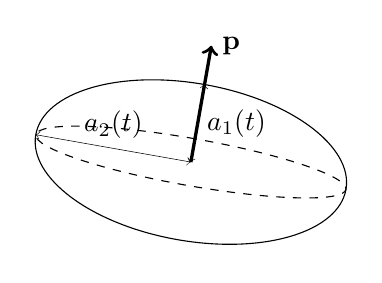
\begin{tikzpicture}[rotate=80]
        \draw(0,0) ellipse (1 cm and 2 cm);
        \draw[dashed](0,0) ellipse (0.3 cm and 2 cm);
        \draw[<->,very thin](0,0) --++ (1,0)node[midway,right]{$a_1(t)$};
        \draw[->,very thick](0,0) --++ (1.5,0)node[right]{$\textbf{p}$};
        \draw[<->,very thin](0,0) --++ (0,2)node[midway,above]{$a_2(t)$};
    \end{tikzpicture}
    \hfill
    \caption{Scheme of an  oblate spheroid oriented along the unit vector \textbf{p} with $a_f(t)$ and $a_2(t)$ the length of the semi axes of the spheroid.
    Note that when the drop is spherical we have $a_f=a_2=a$}
    \label{fig:scheme_spheroid}
\end{figure}

The shape of a particle is entirely described by an orientation vector $\textbf{p}$ and its two semi-axis, $a_1$ and $a_2$.  
By direct integration over the spheroidal particle volume in its local reference frame, i.e. the reference frame formed by $\textbf{p}$ and two other orthogonal unit vectors, it can be shown that $M_1$ and $M_2$ which are the eigenvalues of $\textbf{M}_\alpha$, read as,
\begin{align*}
    M_1 = \frac{m_\alpha a_1^2}{5},
    && M_2 = \frac{m_\alpha a_2^2}{5}.
\end{align*}
Since the particle volume remains constant over time, as given by  \ref{eq:dt_m_alpha}, we can state that $a_2^2 a_1 =a^3$, where $a$ is the radius of the equivalent spherical particle.
To measure the deviation from a spherical shape, we use the dimensionless properties $\chi_I$ and $\chi_{II}$ defined as, $\chi_I = (a_1/a)^2 - 1$ and $\chi_{II} = (a_2/a)^2 - 1$. 
With this definition, $\chi_I = 0$ when, $a_1/a =1$, in other worlds $\chi_I =\chi_{II} = 0$ when the droplet is spherical. 
Thus, $\chi_I$ will be termed the first aspect ratio of the droplet.  
Based on these definitions, the volume conservation condition \eqref{eq:dt_m_alpha} implies that $\chi_{II} = (\chi_I + 1)^{-1/2} - 1$.
% $a_2^2 a_1 =a^3 \to \chi_{II} + 1 = a /a_1$
% $\chi_I = (a_1/a)^2 - 1 \to (\chi_I +1)^{-1/2} = a/a_1$
% $a_1/a = a^2/a_2^2$
% Thus, the droplets shape is entirely determined by its orientation vector and one of its aspect ratio $\chi_I = a_1/a$ or $\chi_{II} = a_2^2/a^2$. 
Considering all these remarks we may describe the droplet shape using the dimensionless tensor, 
\begin{equation*}
    \bm\chi_\alpha
    = \frac{5}{m_\alpha a^2}\textbf{M}_\alpha - \bm\delta
    = \chi_I \textbf{pp}
        +[(\chi_I + 1)^{-1/2} - 1 ] (\bm\delta - \textbf{pp}). 
\end{equation*}
Thus, the droplet spheroidal shape is entirely characterized by two relevant parameters: the orientation vector \textbf{p} and its aspect ratio $\chi_I$.
It is interesting to notice that since $\textbf{p}$ is an eigenvector of $\textbf{M}_\alpha$ and $\bm\chi_\alpha$, $\chi_I$ and $\chi_{II}$ constitute the eigenvalues of $\bm\chi_\alpha$. 
Additionally, note that with the definition used here, $\bm\chi_\alpha +\bm\delta$ corresponds to the Cauchy green deformation tensor often employed in solid mechanics \citep{mwasame2018macroscopic}. 
The geometrical description of the surface of the droplet can also be obtained using the tensor $\bm\chi_\alpha$. 
Indeed, the distance function  $f_\alpha(\textbf{x})$, describing the particle ellipsoidal surface can be defined as \citep{nadim1996concise},  
\begin{equation*}
    f_\alpha(\textbf{x}_\alpha +\textbf{r},t) = \textbf{rr}:(\bm\chi_\alpha +\bm\delta)-a^2.  
    \label{eq:distance_function}
\end{equation*}
It is to be understood from this definition that the points $\textbf{x}$ lying on the surface of the particles respect the constraint $f_\alpha(\textbf{x},t) = 0$. 
Being able to define the droplet's surface in this way will find its use in the calculation of the surface tension stress term present in \ref{eq:dt_S_alpha}. 

% \begin{remark}{Hypothesis of small deformation :}
    
% \end{remark}
\paragraph*{Hypothesis of small deformation: }
A droplet in a pure linear flow will deform into an spheroidal shape \citet{leal2007advanced} at first order in capillary number. 
A buoyant rising droplet with the effect of small inertia will deform at the first order in $Re$ into an ellipsoid as well \citep{taylor1964deformation}.
However, as soon as the inertial effects become higher or the flow quadratic for example, the droplets' deformation is found to exhibit other shapes than spheroidal \citep{taylor1964deformation,stone1990simple}.
Therefore, in this work, we limit our study to small deformations since as soon as the droplet deformation reaches high values one might expect other shapes than ellipsoid, which is in contradiction with the initial assumption. 
Thus, to stay within our study's hypothesis we may consider only small deformation. 
This means that we neglect all the term of $\mathcal{O}(\chi_I^2)$ or $\mathcal{O}(\chi_{II}^2)$ or higher. 
In this situation notice that $\chi_{II} = (\chi_I + 1)^{-1/2} -1 \approx  - \chi_I /2$. 
Thus, the deformation tensor can be written in the simple form, 
\begin{equation}
    \bm\chi 
    = \chi_I
    \left[
        \textbf{pp} 
        - \frac{1}{2}(\bm\delta - \textbf{pp})
    \right]
    = \chi_I \frac{1}{2} \left[
        3 \textbf{pp} - \bm\delta
    \right]
    \label{eq:chi_I_small_def}
\end{equation}
Thus, the trace of $\bm\chi_\alpha$ may be written for small deformation as :  $\bm\delta:\bm\chi_\alpha  = \chi_I + 2\chi_{II} = \mathcal{O}(\chi_{I}^2)$, in other worlds for small deformation $\bm\chi_\alpha$ is purely deviatoric. 
Thus, the trace of $\bm\chi_\alpha$ is null only when considering small deformations. 
This property will be useful in the following sections.
Notice that at the next order of deformation, we have $\bm\delta:\bm\chi_\alpha  = \chi_I + 2\chi_{II} = 3 \chi_I^2 /4 +  \mathcal{O}(\chi_{I}^3)$. 

\subsection{Droplet internal velocity field}

Now that the droplet shape is properly defined we turn our attention to the description of the internal flow present within the droplets.
Indeed, the droplet internal flow $\textbf{w}_d^0$ present in the closure terms of \ref{eq:dt_S_alpha} is not part of the Lagrangian unknown, and therefore must be either directly closed or related to the Lagrangian properties which are part of the unknown of the problem.  
In \citet{lhuillier1987phenomenology} he assumes that the flow within the droplets is linear with the position. 
In our notation, this means that $\textbf{w}_d^0 = \textbf{r}\cdot \textbf{E}_\alpha(t)$ where $\textbf{E}_\alpha(t)$ corresponds to the mean rate of strain of the particle. 
In this case, $\textbf{E}_\alpha(t)$ constitutes an unknown of the particle phase which is solved in \citet{lhuillier1987phenomenology} with an equation similar to \ref{eq:dt_S_alpha}. 
For deformable solid bodies, this approach is accurate since the internal velocity field is indeed linear.
Nevertheless, as discussed in \citet{lhuillier1987phenomenology} for fluid droplets, the internal velocity field $\textbf{w}_d^0$ is far from being linear, as $\textbf{w}_d^0$ exhibits complicated fluid circulation in most of the situations, and this hypothesis is somewhat doubtful. 
Consequently, in this work, we adopt a more general approach that still accounts for the complicated internal flow present inside the particles while using a mean rate of strain tensor, $\textbf{E}_\alpha(t)$, to account for the linear deforming motions. 

It is known that an isolated droplet in creeping flow condition with relative translating motion with the carrier fluid exhibits internal motions. In this specific situation the streamlines formed by $\textbf{w}_d^0$ are known as Hill vortices, see \ref{fig:flowlines1} (b).
In this case $\textbf{w}_d^0$ has a term proportional to \textbf{rr}.  
If slightly more inertial effects are present, the initially spherical droplet deforms into an oblate spheroid \citep{taylor1964deformation}, and one might find that the internal motion of such a spheroid is close to Hill vortexes but with an oblate spheroidal shape, see \ref{fig:flowlines1} (c). 
For a drop immersed in an unbounded pure linear flow, still in stokes flow, we can derive an analytical solution for $\textbf{w}_d^0$ and find that $\textbf{w}_d^0 \sim \textbf{rrr}$ with $\textbf{r}$ the position in space relative to the center of mass of the particle, see \ref{fig:flowlines1} (a), (see \ref{chap:closure-disperse}). 
Thus, in all those cases the internal motions are more complicated than a simple linear velocity field since the internal flow is rather quadratic or cubic. 
Moreover, in all those cases the droplet's internal velocity fields are steady-state solutions.
However, for a droplet to transition from the state depicted in \ref{fig:flowlines1} (b) to the state shown in \ref{fig:flowlines1} (c) it must deform from a sphere to an oblate ellipsoid. 
Equally, a droplet immersed in a pure linear flow may experience deformation, in that case, $\textbf{w}_d^0$ and the shape of the droplet may be a function of time and capillary number \citet[chapter 7]{leal2007advanced}.
\begin{figure*}
    \centering
    \begin{tikzpicture}
        \node (img3) at (0.6\textwidth,0) {\includegraphics[width=0.3\textwidth,angle=270]{image/Rising_def_Stokes.png}};
        \node (img2) at (0.3\textwidth,0) {\includegraphics[width=0.3\textwidth]{image/Rising_Stokes.png}};
        % \draw (0.45\textwidth,0)node{$\rightarrow$};
        % \draw (0.45\textwidth,0.4cm)node{$\bm\Gamma_\alpha\cdot \textbf{r}$};
        \node (img1) at (0.0\textwidth,0) {\includegraphics[width=0.3\textwidth]{image/Shear_Stokes.png}};
        \draw (img3.south)node{(c)};
        \draw (img2.south)node{(b)};
        \draw (img1.south)node{(a)};
    \end{tikzpicture}
    \caption{Three examples of steady state flow lines plots of an isolated droplet immersed into a viscous fluid. 
    (a) Fixed droplet in extensional flow (analytical solution in \ref{chap:daniel2}).
    (b) Rising sphere in uniform stokes flow (analytical solution in \ref{chap:daniel2}). 
    (c) Deformed droplet in rising motion (analytical solution of \citet{taylor1964deformation}). }
    \label{fig:flowlines1}
\end{figure*} 

To account for this deformation in our case we assume that the \textit{transient internal velocity field} which is responsible for this deformation is homogeneous and linear with position \textbf{r}. 
Thus, the \textit{transient internal velocity field} of a particle can be modeled as $\textbf{w}_d^0 = \bm\Gamma_\alpha \cdot \textbf{r}$, where we have introduced, $\bm\Gamma_\alpha$, the mean velocity gradient inside the particle, which symmetric part: $\textbf{E}_\alpha$, represents the rate of strain, and skew-symmetric part: $\bm\Omega_\alpha$, represents the angular velocity. 
Note that the angular velocity tensor $\bm\Omega_\alpha$ is related to the angular velocity \textit{pseudo} vector $\bm\omega_\alpha$ with the relation $\bm\omega_\alpha = -\frac{1}{2}\epsilon_{ijk} (\bm\Omega_\alpha)_{jk}$. 
To summarize, we assume that the inner velocity field of the drop can be decomposed into two distinct parts. 
The first one is the steady-state component, examples are: Hill's vortices for a spherical drop in uniform linear motion, the Hill vortices-like velocity field observed for oblate spheroidal droplets in translation,  the inner velocity field of a drop in steady-state linear flows, and so on.  
The second contribution is the inner velocity fields that alter the drop's shape, this field is assumed linear with the position and homogeneous, it reads  $\bm\Gamma_\alpha\cdot \textbf{r}$. 
Adopting these definitions, the particle's internal velocity is decomposed as, 
\begin{equation}
    \textbf{w}_{d}^0[\textbf{x}_\alpha(t)+\textbf{r},t]
    = \bm\Gamma_{\alpha} \cdot \textbf{r}
    + \textbf{v}^0_{d}[\textbf{r},t]
    =\bm{\Omega}_{\alpha}\cdot \textbf{r}
    + \textbf{E}_{\alpha} \cdot \textbf{r}
    + \textbf{v}^0_{d}[\textbf{r},t]
    \label{eq:def_vel}
\end{equation}
Where we introduced the vector $\textbf{v}^0_d[\textbf{r},t] =\textbf{w}^{0}_{d}[\textbf{x}_\alpha(t)+\textbf{r},t]  - \bm\Gamma_{\alpha}[t] \cdot \textbf{r}$.
With this definition $\textbf{v}_d^0$ represents the particle's internal motion that does not contribute to the linear homogeneous deformation and angular rotation of the drop. 
Thus, $\textbf{v}_d^0$ could be one of the three velocity fields presented in \ref{fig:flowlines1}. 

Due to the consideration of mass conservation \eqref{eq:dt_m_alpha} additional properties can be noted for the tensor $\textbf{E}_\alpha$.
Indeed, at steady-state the local mass conservation inside the particle imposes that $\div \textbf{v}_d^0 = 0$. 
Thus, for a deformable droplet we obtain that $\div \textbf{u}_d^0 = \bm\Gamma_\alpha : \bm\delta = \textbf{E}_\alpha : \bm\delta =  0$.  
Also, note that to preserve the spheroidal shape of the particle we must assume that the particle's rate of strain principal direction is the same as the droplet's shape principal axis. 
In other words, $\textbf{E}_\alpha$ must have the same eigenbasis as $\textbf{M}_\alpha$. 
Making up with these two constrain leads to the expression: $\textbf{E}_\alpha = E_I \textbf{pp} + E_{II} (\bm\delta - \textbf{pp})$, where $E_I$ and $E_{II}$ are the first and second eigenvalue of $\textbf{E}_\alpha$ which are related through $E_I = - 2E_{II}$ due to the volume conservation constraint, ($\bm\delta : \textbf{E}_\alpha =0$). 


Let us now introduce the upper-convected time derivative, also known as the Oldroyd derivative, for an arbitrary Lagrangian second-order tensor $\textbf{A}$ with respect to the mean gradient $\bm\Gamma_\alpha$. 
This derivative is expressed as: 
\begin{equation}
    \overset{\triangledown  }{\textbf{A}}
    = 
    \ddt \textbf{A}
    - \textbf{A} \cdot \bm\Gamma_\alpha
    - \bm\Gamma_\alpha \cdot \textbf{A}
    \label{eq:def_upper}
\end{equation}
The physical interpretation of this operator is that it represents the time derivative of the tensor $\textbf{A}$ in a coordinate system rotating and stretching according to $\bm\Gamma_\alpha$.  
According to our assumption, the droplet shape $\textbf{M}_\alpha$ remains spheroidal under the linear transformation governed by $\bm\Gamma_\alpha$, it is self-similar. 
Additionally, recall that the field $\textbf{r}\cdot \bm\Gamma_\alpha$ accounts for the entire deformation of the droplet. 
Consequently, we deduce that:
\begin{equation}
    \overset{ \triangledown  }{\textbf{M}}_\alpha
    = 0, 
    \label{eq:def_conseq}
\end{equation}
since the shape of the droplet seen in a coordinate system that stretches and rotates with $\bm\Gamma_\alpha$ does not change \footnote{
    This expression is analogous to the definition used in rheology, which states that the upper-convected time derivative of the Finger tensor is always zero.
}.
On the other hand, substituting $\textbf{w}_d^0$ by its definition \eqref{eq:def_vel} in \ref{eq:dt_M_alpha}, gives, 
\begin{equation}
    \ddt \textbf{M}_{\alpha,ik}
    -
    \textbf{M}_{\alpha,ik} \cdot \bm\Gamma_{\alpha,kj}
    -  \bm\Gamma_{\alpha,ki} \cdot \textbf{M}_{\alpha,jk}
    =
    \intO{ 
        (\textbf{v}_{d,i}^0\textbf{r}_j
        + \textbf{r}_i\textbf{v}_{d,j}^0)
    },
\end{equation}
where we have used the Einstein indices summation convention. 
Using the definition of the upper-convected derivative given by \ref{eq:def_conseq}, leads us to the relation,
\begin{equation}
    % \overset{ \footnotesize \triangledown  }{\textbf{M}}_\alpha
    % = 
    \intO{ 
        (\textbf{v}_{d,i}^0\textbf{r}_j
        + \textbf{r}_i\textbf{v}_{d,j}^0)
    }
    =
    0.  
    \label{eq:def_v}
\end{equation}
In summary, the assumption that the droplet shape remains spheroidal and that only the linear velocity field $\textbf{r}\cdot \bm\Gamma_\alpha$ were responsible for the droplet deformation, leads us to the conclusion that $\overset{\triangledown}{\textbf{M}}_\alpha= 0$. 
Then, using the evolution equation for $\textbf{M}_\alpha$ leads us to \ref{eq:def_v}, which can be interpreted as a constraint that the field $\textbf{v}_d^0$ must satisfy. 
Thus, $\textbf{v}_d^0$ is defined by the general relation $\textbf{v}^0_d[\textbf{r},t] =\textbf{w}^{0}_{d}[\textbf{x}_\alpha(t)+\textbf{r},t]  - \bm\Gamma_{\alpha}[t] \cdot \textbf{r}$ and the constraint given by \ref{eq:def_v}. 
One can remark that this constraint is satisfied by each of the solutions represented in \ref{fig:flowlines1}.
This can be verified for the case (a) and (b) with the analytical solution provided in \ref{chap:closure-disperse}. 



% Likewise, $\textbf{v}_d^0$ is assumed not to affect the particle's angular momentum, as the kinematic description of the angular momentum is solely based on its angular velocity $\bm\Omega_\alpha$, just as $\textbf{E}_\alpha$ is assumed to be the only source of deformation. 
% The kinematic description of the angular momentum relies solely on the particle's angular velocity.
% This assumption means that the velocity decomposition has the desirable property that: $\textbf{P}_\alpha = \bm\Gamma_\alpha \cdot \textbf{M}_\alpha + \intO{\textbf{v}^0_{d,i} \textbf{r}_j} =  \bm\Gamma_\alpha \cdot \textbf{M}_\alpha $, at all times, since $\textbf{v}^0_{d,i} $ is not supposed to contribute to either the angular momentum or the symmetric part of the momentum. 
% As it will be shown this simplifies the equations of motion without entirely neglecting the internal motion.
% This means that $\textbf{v}^0_{d}$ can depend on the current shape of the particle through $\textbf{M}_\alpha$ or $\bm\chi_\alpha$ (as shown in \ref{fig:flowlines1} (c)) or its current center of mass velocity $\textbf{u}_\alpha$ (since the Magnitude of Hill vortex depends on the particle center of mass velocity), however, it must satisfy the condition $\intO{\textbf{v}^0_{d,i} \textbf{r}_j}  = 0$.



As demonstrated in \ref{chap:closure-disperse} the internal motions of an isolated spherical drop, such as the one presented in  \ref{fig:flowlines1}, are entirely determined  from $\textbf{u}_f$,$\grad\textbf{u}_f$ and $\textbf{u}_\alpha$ and the shape of the particle. 
Therefore, it is reasonable to assume that in a more general case, $\textbf{v}_d^0$ might be entirely determined by the carrier fluid and particles' properties, specifically, $\textbf{u}_\alpha$ $\textbf{M}_\alpha$, $\textbf{u}_f$ and $\grad\textbf{u}_f$. 
For non-dilute flows we might even, need to consider the volume fraction $\phi_d$ or more complicated functions.
However, this chapter will not delve into these considerations and will focus solely on dilute scenarios.
From now on we consider that the internal velocity $\textbf{v}^0_d(t,\textbf{r})$ is not part of the particle' unknown, but rather as a closure term that should be expressed in terms of $\textbf{u}_\alpha$ $\textbf{M}_\alpha$, $\textbf{u}_f$ and $\grad\textbf{u}_f$. 
Consequently, in this problem, we will explore and demonstrate how a single droplet can be exhaustively described by the parameters, $\textbf{x}_\alpha, \textbf{u}_\alpha, \bm\chi_\alpha$ and $\bm\Gamma_\alpha$, while accounting for more complex internal motion inside the droplets through different closure terms.
As we have seen $\bm\chi_\alpha$ and $\bm\Gamma_\alpha$ may also be replaced by the scalars $\chi_I$, $E_I$ and the vector \textbf{p} and $\bm\omega_\alpha$. 

\subsection{Conservation equations}

Now that the particle's shape and internal kinematics are properly defined we may simplify the moments of mass and momentum equations. 
The integrals appearing in \ref{eq:dt_M_alpha}, \ref{eq:dt_mu_alpha} and \ref{eq:dt_S_alpha} can be reformulated using the definition of $\textbf{w}_d^0$ adopted in \ref{eq:def_vel}, to find, 
\begin{align}
    \textbf{M}_\alpha 
    = \intO{ \rho_d \textbf{rr} }
    = \frac{m_\alpha a^2}{5} (\bm\chi_\alpha+\bm\delta)\\
    % \textbf{P}_\alpha = \textbf{M}_{\alpha,ik} \cdot \bm\Gamma_{\alpha,jk}\\
    \bm\mu_\alpha 
    = \intO{ \rho_d \textbf{r}\times\textbf{u}_d^0 }
    = \textbf{I}_\alpha \cdot \bm\omega_\alpha
    + \intO{ \rho_d \textbf{r}\times\textbf{v}_d^0 }
    \\
    \label{eq:S_def}
    \textbf{S}_{\alpha,ij} = \intO{(\textbf{rw}_ 2^0 )_{ij}+ (\textbf{w}_d^0 \textbf{r})_{ij}} 
    = \textbf{M}_{\alpha,ik} \cdot \bm\Gamma_{\alpha,jk}
        +  \bm\Gamma_{\alpha,ik} \cdot \textbf{M}_{\alpha,jk}
    \\
    \intO{\rho_d \textbf{v}_{d,i}^0\textbf{v}_{d,j}^0}
    = \bm\Gamma_{\alpha,jl}\bm\Gamma_{\alpha,ik} \textbf{M}_{\alpha,kl}  
    +\intO{\rho_d \textbf{v}_{d,i}^0\textbf{v}_{d,j}^0}
    \label{eq:ww_def}
    \\
    \label{eq:sigma_d_def}
    \intO{\bm\sigma_{d,ij}^0}
    =
    2 \mu_d v_\alpha \textbf{E}_{\alpha,ij}
    - \intO{p_d^0} \bm\delta_{ij}
    + \mu_d \intS{(\textbf{n}_i \textbf{v}_{d,j}^0 + \textbf{n}_j \textbf{v}_{d,i}^0)}
    \\
    \intS{\bm\sigma_{I,ij}^0}
    = \frac{\gamma v_\alpha }{a} \left[
        2\bm\delta_{ij} 
        + \frac{4  }{5} \bm\chi_{\alpha,ij}
    \right]
    +\mathcal{O}(|\bm\chi_\alpha|^2)
    % s_\alpha 
    % = 4\pi a^2 (1+\frac{\textbf{M}:\textbf{M}}{15})
\end{align}
where we have introduced the \textit{inertia moment} of the particle $\alpha$ as $\textbf{I}_\alpha = (\bm\delta : \textbf{M}_\alpha)\bm\delta - \textbf{M}_\alpha$. 
These expressions are rather straightforward since one only needs to use the definition of $\textbf{w}_d^0$ in these integrals. 
However, the surface tension stress tensor, $\intS{\bm\sigma_{I,ij}^0}$, is not so easy to obtain since it requires carrying an integral over the spheroidal surface of the particle.
Thus, the detailed calculation of the surface tension stress tensor is given in \ref{ap:surface_tension}. 
We provide the exact results as well as the Taylor expansion of this formula for small deformation. 
Notice that the spheroidal shape remains valid only for small deformations; therefore, the exact formula for $\intS{\bm\sigma_{I,ij}^0}$ considering arbitrary deformation is of limited interest. 
It is good to notice that our formula agrees with the one derived by \citet{lhuillier1987phenomenology} but with the addition of the higher order term not present in this study. 
Additionally, we can observe that two new integrals terms appeared on the right-hand side of \ref{eq:sigma_d_def}  and \ref{eq:ww_def}. 
They correspond respectively to the particle internal viscous stress and the particle internal inertial motions generated by $\textbf{v}_d^0$.
As discussed in the preceding subsection, these contributions arise from motions that are independent of particle deformation and rotation and must be treated as closure terms. 



Injecting these formulas inside \ref{eq:dt_M_alpha}, \ref{eq:dt_mu_alpha}, \ref{eq:dt_S_alpha} yields an equation for $\bm\chi_\alpha$, $\bm\omega_\alpha$ and $\textbf{E}_\alpha$, namely,
\begin{align}
    % \ddt \textbf{pp}_{\alpha,ij}
    % = \textbf{pp}_{\alpha,ik} \cdot \bm\Omega_{\alpha,jk}
    % +  \bm\Omega_{\alpha,ik} \cdot \textbf{pp}_{\alpha,jk}\\
    \overset{ \triangledown  }{\bm\chi}_\alpha
    = 
    \ddt \bm\chi_{\alpha,ij}
    -\bm\chi_{\alpha,ik} \cdot \bm\Gamma_{\alpha,jk}
    - \bm\Gamma_{\alpha,ik} \cdot \bm\chi_{\alpha,jk}
    =
    2\textbf{E}_{\alpha,ij},
    \label{eq:dt_M2}
    \\
    \ddt (\textbf{I}_{\alpha,ik}\bm\omega_{\alpha,k} )
    = 
    \intS{(\textbf{r}\times\bm\sigma_f^0\cdot \textbf{n})_i}
    - \ddt\intO{\rho_d(\textbf{r}\times \textbf{v}_d^0)_i},
    \label{eq:dt_mu2}
    \\
    \ddt \textbf{S}_{\alpha,ij}
    -  \bm\Gamma_{\alpha,jl}\bm\Gamma_{\alpha,ik} \textbf{M}_{\alpha,kl}  
    + \mu_d v_\alpha 2\textbf{E}_{\alpha,ij}
    + \frac{\gamma v_\alpha }{a} \left(
    2\bm\delta_{ij} 
    + \frac{4 }{5} \bm\chi_{\alpha,ij}
    \right) \nonumber\\
    = 
    \frac{1}{2}\intS{(\textbf{r}\bm\sigma_f^0 + \bm\sigma_f^0\textbf{r})_{ijk}\cdot \textbf{n}_k} 
    + \intO{\rho_d \textbf{v}_{d,i}^0\textbf{v}_{d,j}^0}
    + \bm\delta_{ij}\intO{p_d^0} \nonumber\\
    - \mu_d \intS{(\textbf{n}_i \textbf{v}_{d,j}^0 + \textbf{n}_j \textbf{v}_{d,i}^0)},
    \label{eq:dt_S2}
\end{align}
respectively. 
The second moment of mass \ref{eq:dt_M2}, represents the kinematic equation describing the evolution of $\bm\chi_\alpha$ due to the particle elongation and rotation. 
Note that this expression is consistent with the equation obtained by \citet{goddard1967nonlinear} if one accounts for the slightly different definitions of $\bm\chi_\alpha$ and \textbf{C} in \citet{goddard1967nonlinear}.
Following \citet{goddard1967nonlinear} the left-hand side term of \ref{eq:dt_M2} is identified as the upper-convected derivative of $\bm\chi_\alpha$, which returns the rate of strain $\textbf{E}_\alpha$. 
The equation for the skew-symmetric part of the first moment of momentum \ref{eq:dt_mu2}, is the angular momentum balance of the particle when considering the moment of inertia of a deformable particle.
Notice that in this expression the moment of inertia $\textbf{I}_\alpha$ arises naturally since its use simplifies the expression. 
The first term on the right-hand side of \ref{eq:dt_mu2} accounts for the hydrodynamic torque contribution due to the surrounding fluid.
And, the second term represents the changes of angular momentum generated by inner velocity currents. 
The symmetric part of the moment of momentum equations \ref{eq:dt_S2} is an equation for the rate of deformation, $\textbf{E}_\alpha$. 
The first two terms on the left-hand side correspond to the inertial contribution of the mean droplet rate of deformation $\textbf{E}_\alpha$. 
The third term corresponds to the contribution of the droplet's internal stress generated due to the mean drop deformation. 
The last term on the left-hand side is the contribution from the surface tension force which is the only reason why the droplet shape reaches a spherical shape equilibrium. 
These terms are directly related to either $\bm\chi_\alpha$, $\bm\omega_\alpha$ or $\textbf{E}_\alpha$, our unknowns, therefore they are gathered on the left-hand side of the equation. 
On the right-hand side of the equation, we gathered every forcing term, or closure term that is not explicitly a function of the droplet's current shape or deformation.  
The first term is the first moment of the external hydrodynamic forces, $\intS{(\textbf{r}\bm\sigma_f^0+ \bm\sigma_f^0\textbf{r})\cdot \textbf{n}}$ which is a function of the external flow properties but also of the current droplet properties. 
The second forcing term comes from the internal droplet inertia, that is the inertia related to the internal circulation of the drop. 
The third term is the mean droplet's hydrostatic pressure which is balanced mainly by the isotropic part of the surface tension contribution and the mean fluid pressure. 
The last term on the right-hand side then corresponds to the internal viscous stress generated by the relative motion of the drop with the carrier fluid. 


From \ref{eq:dt_D_alpha} we can also derive a conservation for the trace of $\bm\Gamma_\alpha$ it reads, 
\begin{equation}
    -  \bm\Gamma_{\alpha,ml}\bm\Gamma_{\alpha,mk} \textbf{M}_{\alpha,kl}  
    + \frac{\gamma v_\alpha }{a} 
    \left[
    2\bm\delta_{mm} 
    % - \frac{4 }{5 } (\textbf{M}_{\alpha,mm}^* - \textbf{I}_{\alpha,mm})
    \right]
    = 
    \intS{\textbf{r}_m\cdot\bm\sigma_{1,mk}^0\cdot \textbf{n}_k} 
    + \intO{\rho_d \textbf{v}_{d,m}^0\cdot \textbf{v}_{d,m}^0}
    + \intO{p_d^0} \bm\delta_{mm},
    \label{eq:dt_trM2}
\end{equation}
This equation, corresponds to a scalar equation describing the dynamical balance of the isotropic part of the moment of momentum of the particle. 
This equation contains the trace of every term present in \ref{eq:dt_S2} except that both viscous terms and the derivative of the trace of $\textbf{S}_\alpha$ canceled since they are traceless tensors. 
Notice that the second term on the left-hand side is the isotropic part of the surface tension forces, it corresponds to the well-known Laplace pressure. 
Additionally, on the right-hand side of \ref{eq:dt_trM2} we notice the trace of the hydrodynamic forces, which together with the particle internal pressure form the Laplace equation. 
Nevertheless, \ref{eq:dt_trM2} is more general than the classic Laplace equilibrium equation as it includes inertial effects as well as particle internal motions and deformations effects.  
Initially, \ref{eq:dt_trM2} is supposed to be used as an equation for $M_\alpha$, or more precisely the trace of $\bm\chi_\alpha$.
However, since the particle volume is assumed constant, \ref{eq:dt_trM2} can be considered as an equation for the particle mean internal pressure. 
Indeed, using that expression to cancel out the particle pressure in \ref{eq:dt_S2} gives us a novel expression that describes the deviatoric part of $\textbf{M}_\alpha$ or $\bm\chi_\alpha$.
Therefore, it corresponds to the description of the deviation from the spherical particle's shape $\bm\chi_{\alpha,ij}$. 
Indeed, injecting \ref{eq:dt_trM2,eq:dt_M2,eq:S_def} into  \ref{eq:dt_S2} one obtain, 
\begin{align}
        \frac{1}{2}\ddt^2 \bm\chi_{\alpha,ij}
        - (\bm\chi_{\alpha,kl} + \bm\delta_{kl})
        (\bm\Gamma_{\alpha,jl}\bm\Gamma_{\alpha,ik}  
        - \frac{1}{3}
        \bm\Gamma_{\alpha,ml}\bm\Gamma_{\alpha,mk}  
        \bm\delta_{ij}
        )
    &+ 
    \overset{ \triangledown  }{\bm\chi}_\alpha
    / \tau_\mu
    +
    \bm\chi_{\alpha,ij}
    / \tau_\gamma^2
    = 
    \textbf{F}_{ij}
    \label{eq:dev}
\end{align}
where,
\begin{align}
    1/\tau_\mu 
    =
    \frac{\mu_d 10}{\rho_d a^2}  
    &&
    1/\tau_\gamma^2
    = 
    \frac{\gamma 8 }{\rho_d a^3} 
\end{align}
and,
\begin{align}
    \textbf{F}_{ij}
    &= 
    \textbf{F}_{ij}^h
    +\textbf{F}_{ij}^{vv}
    + \textbf{F}_{ij}^{\sigma}\\
    \textbf{F}_{ij}^h
    &= \frac{10}{2m_\alpha a^2}\intS{(\textbf{r}\bm\sigma_f^0 + \bm\sigma_f^0\textbf{r} - \frac{2}{3}(\textbf{r}\cdot \bm\sigma_f^0) \bm\delta)\cdot \textbf{n}} \\
    \textbf{F}_{ij}^{vv}
    &= 
    \frac{10 \rho_d}{m_\alpha a^2}\intO{(\textbf{v}_{d,i}^0\textbf{v}_{d,j}^0 - \frac{1}{3}\textbf{v}_{d,m}^0\textbf{v}_{d,m}^0 \bm\delta_{ij}) }\\
    \textbf{F}_{ij}^{\sigma}
    &= - \frac{ 10 \mu_d}{m_\alpha a^2} \intS{(\textbf{n}_i \textbf{v}_{d,j}^0 + \textbf{n}_j \textbf{v}_{d,i}^0)}\nonumber
\end{align}
where we have gathered all the closures or forcing terms into the tensor $\textbf{F}_{ij}$ which has the unit [s$^{-2}$]. 
% Notice that $\textbf{E}_{\alpha,ij}$ is related to the \textit{convected} derivative of $\bm\chi_\alpha$ through \ref{eq:dt_M2}. 
One might recognize in \ref{eq:dev} a forced second-order oscillatory harmonic equation.
Indeed, the left-hand side terms correspond to the second, first and zeroth order derivative of $\bm\chi$ (i.e. $\ddt^2 \bm\chi_{\alpha,}$, $\overset{ \triangledown  }{\bm\chi}_\alpha$ and $\bm\chi_\alpha$ respectively), with the addition of the non-linear term, $ (\bm\chi_{\alpha,kl}+\bm\delta_{kl}) 
(\bm\Gamma_{\alpha,jl}\bm\Gamma_{\alpha,ik}  
- \frac{1}{3}
\bm\Gamma_{\alpha,ml}\bm\Gamma_{\alpha,mk}  
\bm\delta_{ij}
)$, while the right-hand side terms correspond to the forcing terms. 

Although oscillatory harmonic equations are typically scalar, this formulation is more general and holds for the deformation tensor. 
Notably, the coefficients $\tau_\mu$ and $\tau_\gamma$ in \ref{eq:dev} which appear in front of $\overset{ \triangledown  }{\bm\chi}_\alpha$ and $\bm\chi_\alpha$ respectively, correspond precisely to the damping ratio and the square of the natural frequency of the secondary mode of oscillation for nearly spherical droplets, as described by \citep{lamb1924hydrodynamics}. 
Indeed, in the case of freely oscillating droplets, the natural time governing the period of oscillation of droplet deformation is given by $\tau_\gamma = \sqrt{\frac{a^3\rho_d}{8 \gamma }}$ \citep{lamb1924hydrodynamics}. 
Likewise, the damping coefficient, which corresponds to the timescale over which oscillations decay, is given by  $\tau_\mu = a^2\rho_d/10 \mu_d$ \citep{lamb1924hydrodynamics}. 


To conclude, the system of equations formed by \ref{eq:dt_M2}, \ref{eq:dt_mu2} and \ref{eq:dev}, with unknown $\bm\chi_\alpha$, $\textbf{E}_\alpha$ and $\bm\omega_\alpha$, allows us to describe the deformation and the rate of deformation of a spheroidal droplet with constant volume.

\subsection{The dimensionless equations}


To enhance the physical understanding of \ref{eq:dev} we derive in the present section the dimensionless form of this equation. 
We introduce the timescale, $\tau$ which represents the droplet's natural time of deformation rate in the absence of external influences.
It is important to note that these scalings are specific to the particular scenarios described and are not applicable to general situations. 
Consequently, we consider $\tau$ as the characteristic timescale for droplet deformation, acknowledging that its exact definition remains context-dependent.
Meaning that for example, $|\ddt^2 \bm\chi_{\alpha,ij} |\sim 1/\tau^2$ and $ \overset{ \triangledown  }{\bm\chi}_\alpha \sim 1/\tau$. 
\tb{in fact that is not true $\pddt \sim 1/ \tau_u$ in podzrikidis}

Additionally, we assume that the forcing terms introduced in \ref{eq:dev} are governed by a timescale independent of the droplet's natural timescale, denoted as $\tau_u$. 
This is because the external solicitation timescale is imposed by the ``background flow'' condition and thus is quite independent of the current droplet rate of deformation. 
For example, the term $\textbf{F}_{ij}^{vv}$ representing the kinetic energy of the internal droplet velocity, is mainly driven by the relative velocity between the droplet's center of mass and the background flow. 
In fact in \ref{chap:closure-disperse} we compute this term in the situation represented in \ref{fig:flowlines1} (b) and show that $ \textbf{F}^{vv}\sim (\textbf{u}_f - \textbf{u}_p)(\textbf{u}_f - \textbf{u}_p)$. 
Thus, in this case, the timescale of the forcing term is given by $\tau_u = a /(\textbf{u}_f - \textbf{u}_p)$. 
This means that the Hill vortices velocity in \ref{fig:flowlines1} (b) are driven by the velocity scale $\textbf{u}_f - \textbf{u}_p$ and therefore the term $\textbf{F}^{vv}$ scale as $1/\tau_u^2$. 
If the ``background flow'' is not uniform but linear or represents isotropic turbulence, the principle stays the same and $\tau_u$ will be related to the background flow timescale. 
Consequently, the forcing terms can be defined proportional to the scales: 
\begin{align*}
    \textbf{F}_{ij}^h
    &= \frac{1}{2v_\alpha}\intS{(\textbf{r}\bm\sigma_f^0 + \bm\sigma_f^0\textbf{r} - \frac{2}{3}(\textbf{r}\cdot \bm\sigma_f^0) \bm\delta)\cdot \textbf{n}} 
    \sim \mu_f  /\tau_u \\
    \textbf{F}_{ij}^{vv}
    &= \frac{\rho_d}{v_\alpha}
    \intO{(\textbf{v}_{d,i}^0\textbf{v}_{d,j}^0 - \frac{1}{3}\textbf{v}_{d,m}^0\textbf{v}_{d,m}^0 \bm\delta_{ij}) }
    \sim  \rho_d a^2  /\tau_u^2 \\
    \textbf{F}_{ij}^{\sigma}
    &= - \frac{\mu_d}{v_\alpha} \intS{(\textbf{n}_i \textbf{v}_{d,j}^0 + \textbf{n}_j \textbf{v}_{d,i}^0)}
    \sim  \mu_d  /\tau_u. 
\end{align*}
Where it has been assumed that the term $\textbf{F}_{ij}^h$ scale as a viscous force. 
Re-writing \ref{eq:dt_trM2} considering these scales yields the dimensionless tensor equation, 
\begin{multline}
    \frac{\zeta Re \beta^2}{5}
    \left[
        \frac{1}{2}\ddt^2 \bm\chi_{\alpha,ij}
        -   (\bm\chi_{\alpha,kl} + \bm\delta_{kl})
        (\bm\Gamma_{\alpha,jl}\bm\Gamma_{\alpha,ik}  
        - \frac{1}{3}
        \bm\Gamma_{\alpha,ml}\bm\Gamma_{\alpha,mk}  
        \bm\delta_{ij}
        )
    \right]\\
    + \lambda \beta \overset{ \triangledown  }{\bm\chi}_\alpha
    + \frac{1}{Ca}
    \frac{4  }{5} \bm\chi_{\alpha,ij}
    = (\textbf{F}_{ij}^h )^*
    + \zeta Re (\textbf{F}_{ij}^{vv})^*
    + \lambda (\textbf{F}_{ij}^{\sigma})^* 
    \label{eq:dev_dim}
\end{multline}
where we have defined the following dimensionless groups : 
\begin{align*}
    \beta = \frac{\tau_u}{\tau},
    && \zeta = \rho_d /\rho_f,
    && \lambda = \mu_d/\mu_f,
    && Re = \frac{\rho_f a^2 }{ \mu_f \tau_u},
    && Ca = \frac{a \mu_f}{\gamma \tau_u}. 
\end{align*}
The superscript $^*$ indicates that the argument is made dimensionless. 
Each of these dimensionless numbers has a distinct physical signification. 
Let us start with $\beta$, this number compares the typical timescale of the external contribution with the natural timescale of the droplets' deformation.
$\zeta$ is the ratio of the carrier fluid density to the droplet density. 
$\lambda$ is the ratio of the carrier fluid viscosity to the droplet viscosity. 
The number $Re$ compares the viscous forces to inertial forces. 
And $Ca$ is the ratio of the capillary forces compared to the viscous forces. 
Thus, on the left-hand side of \ref{eq:dev_dim} we identify the inertial terms; (the terms factor of $Re$), the viscous terms (i.e. the terms factor of $\lambda$) and the surface tension or capillary contribution which are factor of $1/Ca$. 
The same comments can be made regarding the forcing terms on the right-hand side. 


We will now explore specific regimes where this equation simplifies. To provide a clearer physical understanding, we consider four different scenarios: the low Reynolds number regime, the quasi-steady regime, the bubbly flow regime, and the free-oscillating droplet regime. 


\subsubsection{Free oscillating droplets}

As a first example let us consider a freely oscillating droplet, meaning that we neglect the carrier fluid property. 
This example applies well to viscous droplets in air where the influence of the carrier fluid on the droplet can be completely neglected, meaning that all the forcing terms on the right-hand side of \ref{eq:dev_dim} can be ignored.\footnote{
    Note that even $\textbf{F}^{vv}$ can be neglected since it is the external forcing that induces an internal velocity through the droplet interface motion, hence in the absence of external forcing  $\textbf{F}^{vv}=0$.  
} 
Thus, \ref{eq:dev_dim} reduce to, 
\begin{multline}
    \frac{\zeta Re \beta^2}{5}
    \left[
        \frac{1}{2}\ddt^2 \bm\chi_{\alpha,ij}
        -  ( \bm\chi_{\alpha,kl} +\bm\delta_{kl})
        (\bm\Gamma_{\alpha,jl}\bm\Gamma_{\alpha,ik}  
        - \frac{1}{3}
        \bm\Gamma_{\alpha,ml}\bm\Gamma_{\alpha,mk}  
        \bm\delta_{ij}
        )
    \right]
    + \lambda \beta \overset{ \triangledown  }{\bm\chi}_\alpha
    + \frac{1}{Ca}
    \frac{4  }{5} \bm\chi_{\alpha,ij}
    =
    0.
\end{multline}
In this regime, the droplet shape follows a non-linear homogeneous partial differential tensorial equation. 
As no forcing terms are present in this equation, we can predict that in the steady state $\bm\chi_\alpha = 0$ meaning that the droplet shape will eventually relax into a spherical shape in this regime.
This holds under the condition that $\lambda$ remains finite.   
% In the following we show that, upon linearizing this equation, we recover the second-order free-oscillatory harmonic equations introduced by \citet{lamb1924hydrodynamics}. 

\subsubsection{Low Reynolds number or viscous dominated regime}

Now, let us assume that the relative motion between the droplets and the carrier phase is rather viscous such that $Re \ll 1$.
In this situation \ref{eq:dev_dim} reduces to, 
\begin{equation*}
    % \frac{\zeta Re \beta^2}{5}
    % \left[
    %     \frac{1}{2}\ddt^2 \bm\chi_{\alpha,ij}
    %     -   \textbf{M}_{\alpha,kl} 
    %     (\bm\Gamma_{\alpha,jl}\bm\Gamma_{\alpha,ik}  
    %     - \frac{1}{3}
    %     \bm\Gamma_{\alpha,ml}\bm\Gamma_{\alpha,mk}  
    %     \bm\delta_{ij}
    %     )
    % \right]\\
    \lambda \beta \overset{ \triangledown  }{\bm\chi}_\alpha
    + \frac{1}{Ca}
    \frac{4  }{5} \bm\chi_{\alpha,ij}
    = (\textbf{F}_{ij}^h)^* 
    % + \zeta Re \textbf{F}_{ij}^{vv}
    + \lambda (\textbf{F}_{ij}^{\sigma})^*
    \label{eq:stokes_shape}
\end{equation*}
We can observe that in this regime the shape of the particle is governed by a balance of viscous stress due to the rate of current deformation (first term), the surface tension force (second term), the external hydrodynamic contribution (first term on the right-hand side), and finally the particle's internal viscous stresses generated due to the internal re-circulation (second term on the right-hand side). 
This situation is typically experienced by neutrally buoyant droplets immersed in a shear flow at low $Re$. 
For example in \citet[Chapter 7]{leal2007advanced} they derive the evolution equation for a deformable droplet in a pure linear flow, in this case, this balance should hold. 

\subsubsection{Quasi-steady state regime}

% In certain situations the natural times related to the droplet rate of deformation, $\tau$, is greater than the timescale of the external flow $\tau_u$ which is generally much smaller. 
Let us consider the situation of rising buoyant droplets or bubbles. 
In that case, the external contributions are all proportional to the only relative motion present in homogeneous rising flows which is the relative phase velocity $\textbf{u}_p-\textbf{u}_f$ (or the square of that in inertial regime).
When the droplets reach their terminal rising velocity it is clear that $\tau_u \sim a / \textbf{u}_p-\textbf{u}_f $.
On the other hand, the natural times related to the droplet rate of deformation might be given either by $1 / \tau \sim \sqrt{\frac{ \gamma }{a^3\rho_d}}$ or $\sim  \mu_d  /(a^2\rho_d)$. 
Therefore, the Quasi-steady state assumption, $\beta \ll 1$ requires, 
\begin{equation}
  1/\beta^2 =  \frac{a\rho_d |\textbf{u}_p-\textbf{u}_f|^2}{\gamma } = \zeta We \gg 1 
\end{equation}
Or, 
\begin{equation}
    1/\beta = (a\rho_d|\textbf{u}_p-\textbf{u}_f|)/(\mu_d ) = \frac{\zeta Re }{\lambda} \gg 1
\end{equation}

Thus, in this case, $\beta \ll 1$ and we can neglect the transient effects arising due to the droplets' deformation, which yields, 
\begin{equation}
    % \frac{\zeta Re \beta^2}{5}
    % \left[
    %     \frac{1}{2}\ddt^2 \bm\chi_{\alpha,ij}
    %     -   \textbf{M}_{\alpha,kl} 
    %     (\bm\Gamma_{\alpha,jl}\bm\Gamma_{\alpha,ik}  
    %     - \frac{1}{3}
    %     \bm\Gamma_{\alpha,ml}\bm\Gamma_{\alpha,mk}  
    %     \bm\delta_{ij}
    %     )
    % \right]\\
    % \lambda \beta 2 \textbf{E}_{\alpha,ij}
    \frac{1}{Ca}
    \frac{4  }{5} \bm\chi_{\alpha,ij}
    = (\textbf{F}_{ij}^h)^*
    + \zeta Re (\textbf{F}_{ij}^{vv})^*
    + \lambda (\textbf{F}_{ij}^{\sigma})^*
    \label{eq:steady}
\end{equation}
Consequently, in the quasi-steady-state regime, the droplet deformation is given explicitly by the sum of: the external hydrodynamic contribution; the inertial due to internal particle re-circulation; and the particle internal stresses due to this internal motion. 
Notice that in \citet{taylor1964deformation} they compute the shape of a steady state rising droplet analytically and consider low but finite inertial effects. 
In this case \ref{eq:steady} typically governs the shape balance.
 

\subsubsection{Bubbly flow regime}
Finally, for bubbly flows where the density and viscosity of the bubbles are negligible compared to those of the carrier fluid, we have $\zeta \ll 1$ and $\lambda \ll 0$. 
In this particular situation, the shape equation simplifies significantly to:
\begin{equation}
    % \frac{\zeta Re \beta^2}{5}
    % \left[
    %     \frac{1}{2}\ddt^2 \bm\chi_{\alpha,ij}
    %     -   \textbf{M}_{\alpha,kl} 
    %     (\bm\Gamma_{\alpha,jl}\bm\Gamma_{\alpha,ik}  
    %     - \frac{1}{3}
    %     \bm\Gamma_{\alpha,ml}\bm\Gamma_{\alpha,mk}  
    %     \bm\delta_{ij}
    %     )
    % \right]\\
    % \lambda \beta 2 \textbf{E}_{\alpha,ij}
    \frac{1}{Ca}
    \frac{4  }{5} \bm\chi_{\alpha,ij}
    = (\textbf{F}_{ij}^h)^*. 
    \label{eq:bubbles}
\end{equation}
This implies that the shape of a bubble is entirely determined by the external fluid solicitation. 
The absence of both $\textbf{E}_\alpha$ and the derivative of $\bm\chi_\alpha$ indicates that bubbles adjust their shape instantaneously to the carrier fluid’s forces.

However, it is known that bubbles in water can still exhibit oscillations due to the added mass effect. 
This might seem contradictory to \ref{eq:bubbles} as no second-order derivatives of $\bm\chi_\alpha$ are present in this equation. 
However, the term $\textbf{F}_{ij}^h$ can be proportional to $\ddt^2 \bm\chi_\alpha$ with the proportionality constant being the added mass coefficient, which is related to the first moment of the hydrodynamic forces. 
In that case, the natural oscillation frequency of the bubbles will be related to added mass effects. 

As stated earlier, the spheroidal shape of a particle can be described uniquely using the scalars $\chi_I$ and $E_I$ since the other components of $\bm\chi_\alpha$ and $\textbf{E}_\alpha$ might be entirely deduced from $\chi_I$ and $E_I$, and the orientation vector \textbf{p}. 
Therefore, progress can be made to reduce this system of tensor equations to one equation for \textbf{p}, $\bm\omega_\alpha$ and two scalars equations, one for $\chi_I$ and another for $E_I$. 
This is the purpose of the next subsection. 


\subsection{Local reference frame equations}

In order to derive equations for the scalars $\chi_I$ and $E_I$ we demonstrate here that we need to express \ref{eq:dt_M2} and \ref{eq:dev} in they principal basis, i.e. the basis formed by the eigenvector of $\bm\chi_\alpha$ and $\textbf{E}_\alpha$. 
Since we are not interested in all eigenvalues of $\bm\chi_\alpha$ and $\textbf{E}_\alpha$ but rather only on $\chi_I$ and $E_I$, it is sufficient to project the equations onto the first eigenvector $\textbf{p}$. 

\subsubsection{Preliminaries and orientation equation}
We first introduce the relation,
\begin{equation}
    \bm\chi_{\alpha,ij} \textbf{p}_i\textbf{p}_j
    = 
    (
        \chi_I \textbf{p}_i\textbf{p}_j
        + \chi_{II} (\bm\delta_{ij} - \textbf{p}_i\textbf{p}_j)
    ) \textbf{p}_i\textbf{p}_j
    = \chi_I.
    \label{eq:chi_I_def}
\end{equation} 
This relation simply states that the projection of $\bm\chi_\alpha$ on its first eigenvector $\textbf{p}$, returns (by definition) its first eigenvalue $\chi_I$. 
Likewise, we might show that, 
\begin{equation}
    \textbf{E}_{\alpha,ij} \textbf{p}_i\textbf{p}_j
    = 
    (
        E_I \textbf{p}_i\textbf{p}_j
        + E_{II} (\bm\delta_{ij} - \textbf{p}_i\textbf{p}_j)
    ) \textbf{p}_i\textbf{p}_j
    = E_I.
    \label{eq:E_I_def}
\end{equation} 
Notice that this equation requires that the main axis of deformation occurs in the same direction as the current state of deformation, that is in the direction of $\textbf{p}$. 
As mentioned earlier this assumption is made here, since to preserve the droplet spheroidal shape the deformation must occur along the axis of deformation. 
One might deduce that to derive an equation for $\chi_I$ one just need to multiply \ref{eq:dt_M2} by $\textbf{p}_i \textbf{p}_j$, likewise to obtain an equation for $E_I$ one needs to multiply \ref{eq:dev} by $\textbf{p}_i \textbf{p}_j$. 
Nevertheless, notice that this will make appear the derivative of $\textbf{p}_i \textbf{p}_j$ in the resulting equations, introducing the need of a transport equation for this tensor. 

Therefore, let us focus on the derivation of an equation for the tensor  $\textbf{p}_i \textbf{p}_j$. 
This transport equation is straightforward to obtain if one first notices that due to purely kinematics constraints, any unit vector \textbf{p} follows the kinetic relation $\ddt \textbf{p} = \bm\Omega_\alpha \cdot \textbf{p}$.
Indeed, the angular velocity of \textbf{p} corresponds, by definition, to the particle's angular velocity. 
Taking the time derivative of $\textbf{pp}$ and using the chain rule directly yields the relation, 
\begin{equation}
    \ddt (\textbf{pp})_{ij}
    = 
    (\textbf{pp})_{ik}\cdot\bm\Omega_{\alpha,jk}. 
    +\bm\Omega_{\alpha,ik}\cdot (\textbf{pp})_{jk}
    \label{eq:dt_pp}
\end{equation}
Notice that this equation is extensively used in fiber media theory to predict the evolution of fiber orientation in a medium. 
% This equation constitutes the theoretical ground from which all Folgar-Tukers-like models are derived. 
% This will be discussed in the next section.

\subsubsection{Local reference frame kinematic equation}

Now that the basic relations are derived let us focus on the derivation of the equation for $\chi_I$. 
Multiplying \ref{eq:dt_M2} by $(\textbf{pp})_{ij}$ and using \ref{eq:chi_I_def},\ref{eq:E_I_def} and  \ref{eq:dt_pp} gives, 
\begin{equation}
    \ddt \chi_I
    = 
    \bm\chi_{\alpha,ij} [(\textbf{pp})_{ik}\cdot\bm\Omega_{\alpha,jk}. 
    +\bm\Omega_{\alpha,ik}\cdot (\textbf{pp})_{jk}]
    + (\textbf{pp})_{ij}(\bm\chi_{\alpha,ik} \cdot \bm\Gamma_{\alpha,jk}
    + \bm\Gamma_{\alpha,ik} \cdot \bm\chi_{\alpha,jk}
    + 2\textbf{E}_{\alpha,ij})
    \label{eq:step_one}
\end{equation}
The product $\bm\chi_{ij} (\textbf{pp})_{ik}$ and $(\textbf{pp})_{ij}\bm\chi_{\alpha,ik}$ both gives, 
\begin{equation*}
    \bm\chi_{ij} (\textbf{pp})_{ik}
    =
    (\textbf{pp})_{ij}\bm\chi_{\alpha,ik}
    = 
    \chi_I (\textbf{pp})_{jk}
\end{equation*}
and so on for $\bm\chi_{ij} (\textbf{pp})_{jk}$ and $(\textbf{pp})_{ij} \bm\chi_{\alpha,jk}$. 
Thus, the right-hand side of \ref{eq:step_one} may be written as, 
\begin{equation}
    \ddt \chi_I
    = 
    \chi_I [(\textbf{pp})_{jk}:(\bm\Omega_{\alpha,jk} + \bm\Gamma_{\alpha,jk}). 
    +(\bm\Omega_{\alpha,ik} + \bm\Gamma_{\alpha,ik}) :(\textbf{pp})_{ik}]
    + 2E_I
    \label{eq:step_two}
\end{equation}
One might directly notice that the skew-symmetric part of $\bm\Gamma_\alpha$ and the tensor $\bm\Omega_\alpha$ vanish due to the double contracted product with the symmetric tensor $\textbf{pp}$. 
This finally gives 
\begin{equation}
    \ddt \chi_I
    = 
    2(\chi_I +1)E_I. 
    \label{eq:dt_chi_I}
\end{equation}
This equation simply states that the derivative of the deformation corresponds to the rate of strain in that same direction time the current deformation plus one.  
Rearranging this equation one can equally show that $2E_I = \ddt (\ln(\chi_I+1))$ which for small deformations gives,
\begin{equation}
    2E_I =  \ddt \chi_I + \mathcal{O}(\chi_I^2). 
    \label{eq:small_def}
\end{equation}
The absence of $\bm\Omega_\alpha$ indicates that in the local basis of the particle, the rotation of the latter does not impact the kinematic relation between the deformation $\chi_I$ and the rate of deformation $E_I$.
This is easily understandable as it is a kinematic relation. 
In contrast, the particle's rotation plays a significant role in the particle's dynamical balance equations.


\subsubsection{Local reference frame dynamic equations}
% \subsubsection{The local reference frame rate of strain equations}

Now we apply the same reasoning on the rate of strain conservation \eqref{eq:dt_S2} and angular momentum conservation \eqref{eq:dt_mu_alpha},
by multiplying each terms on the left-hand side of \ref{eq:dt_S2} and \ref{eq:dt_mu_alpha} by $(\textbf{pp})_{ij}$. 
As the mathematical derivation is more lengthily, the details are presented in \ref{ap:local_basis_eq}. 
Note that in \ref{ap:local_basis_eq} we demonstrate how to project an equation or tensor on its $3$ eigenvectors, not only the first one ($\textbf{p}$). 
To accomplish such a task we have to introduce the \textit{local basis notations}. 
Let us consider the local basis $\{\textbf{p}^0, \textbf{p}^1, \textbf{p}^2\}$ which constitutes an orthonormal eigenbasis of both the tensors $\bm\chi_\alpha$ and $\textbf{E}_\alpha$. 
It must be understood here that $\textbf{p}^0 = \textbf{p}$. 
Then, any second-order tensor $A_{ij}$ can be written in the form, 
\begin{equation*}
    (\textbf{A})_{ij}
    = 
    \sum_{a,b =1}^3
    (A^{ab} \textbf{p}^a\textbf{p}^b)_{ij}
    = 
    \sum_{a,b =1}^3
    A^{ab} p_i^ap_j^b,
\end{equation*}
where $A^{ab}$ are the scalar components of the tensor \textbf{A} in the local basis  $\{\textbf{p}^0, \textbf{p}^1, \textbf{p}^2\}$. 
If $\{\textbf{p}^0, \textbf{p}^1, \textbf{p}^2\}$ constitutes an eigenbasis of the tensor \textbf{A} then the off diagonal components $A^{ab}$ with $a\neq b$ all vanish. 
Thus, one is left with the formula, 
\begin{equation*}
    A_{ij}
    = 
    \sum_{a =1}^3
    A^{aa} p_i^ap_j^a. 
\end{equation*}
Where the $A^{aa}$ are the eigenvalues of the tensor \textbf{A}. 
Particularly, since $\{\textbf{p}^0, \textbf{p}^1, \textbf{p}^2\}$ is the eigenbasis of $\bm\chi_\alpha$ and $\textbf{E}_\alpha$ we can write, 
\begin{align*}
    (\bm\chi_\alpha)_{ij}
    =
    \sum_{a =1}^3
    (\chi^{aa} \textbf{p}^a\textbf{p}^a)_{ij}. 
    =
    \chi_I  p_i^0p_j^0
    + \chi_{II}  p_i^1p_j^1
    + \chi_{II}  p_i^2p_j^2. \\
    (\textbf{E}_\alpha)_{ij}
    =
    \sum_{a =1}^3
    (E^{aa} \textbf{p}^a\textbf{p}^a)_{ij}. 
    = 
    E_I  p_i^0p_j^0
    + E_{II}  p_i^1p_j^1
    + E_{II}  p_i^2p_j^2. \\
\end{align*}


Additionally, the tensor $\bm\Omega_\alpha$, even though not diagonal in the basis  $\{\textbf{p}^0, \textbf{p}^1, \textbf{p}^2\}$ can be written as, 
\begin{equation*}
    \Omega_{\alpha,ij}
    = 
    \sum_{a,b=1}^3
    \Omega^{ab}_\alpha p_i^ap_j^b. 
\end{equation*}
Where $\Omega_\alpha^{ab} = \bm\omega_\alpha : \textbf{p}^b\textbf{p}^a$ are the components of $\bm\Omega_\alpha$ in the basis $\{\textbf{p}^0, \textbf{p}^1, \textbf{p}^2\}$. 
Likewise, the pseudo vector $\bm\omega_\alpha$ can be express as, 
\begin{equation*}
    \bm\omega_{\alpha,i}
    = 
    \sum_{a=1}^3
    \bm\omega_\alpha^a p_i^a. 
\end{equation*}
Where $\omega_\alpha^a = \bm\omega_\alpha \cdot \textbf{p}^a$ are the components of $\bm\omega_\alpha$ in the basis $\{\textbf{p}^0, \textbf{p}^1, \textbf{p}^2\}$. 



\paragraph*{Angular momentum equation:}
As demonstrated in \ref{ap:local_basis_eq} taking the dot product of \ref{eq:dt_mu2} with $\textbf{p}^i$ gives directly the momentum balance of a single particle in its matrix of inertia local basis. 
The evolution of the $a^{th}$ component of the angular velocity vector in the basis $\{\textbf{p}^0, \textbf{p}^1, \textbf{p}^2\}$ can then be written as, 
\begin{equation}
    \ddt\omega^a_\alpha
    = 
    % I^{ab}\omega^b  \omega^c \epsilon_{jki} p_i^a p_j^c p_k^a
    \frac{5}{m_\alpha a^2 (2 - \chi_I)}
    \left[
    \omega^a E^a 
    +
    \textbf{p}^a \cdot \left(
        \intS{(\textbf{r}\times\bm\sigma_f^0\cdot \textbf{n})} 
        - \ddt\intO{\rho_d(\textbf{r}\times \textbf{v}_d^0)}
    \right)
    \right].  
    \label{eq:dt_omega_a}  
\end{equation}
It is important to note that this equation applies separately for each $i = 0,1,2$, thus, this remains a vector equation. 
The first term on the right-hand side appears due to the change of reference frame and is caused by the rate of deformation of the particle.
Note that this term vanishes for solid particles, indeed $E^i = 0$ for unreformable particles. 
The second source term on the right-hand side represents the hydrodynamic torque vector projected onto the axis $\textbf{p}^i$. 
Similarly, the last term corresponds to the rate of changes of the internal angular momentum, projected onto axis $\textbf{p}^i$. 
% Additionally, the absence of the inertia matrix within the derivative on the left-hand side, makes the equation considerably easier to solve.
% In the limit of small deformation, we may reformulate the first term on the right-hand side using the approximation, 
% $
%     \frac{1}{(2-\chi_I)} \frac{1}{2} E_I 
%     = \frac{E_I}{2}
% $
% which gives the angular momentum for small deformation as, 
% \begin{align*}\textsc{
%     \ddt\omega^i 
%     = 
%     % I^{ab}\omega^b  \omega^c \epsilon_{jki} p_i^a p_j^c p_k^a
%     \frac{5}{ 2 m_\alpha a^2}
%     \left(
%     \omega^i E^i
%     +
%     \frac{\textbf{p}^i}{2 - \chi_I}\cdot \intS{(\textbf{r}\times\bm\sigma_f^0\cdot \textbf{n})_i} 
%     \right).    
%     \label{eq:dt_omega_I}
% \end{align*}}
We obtained a vector equation for the angular rotation vector in the eigenbasis of the particle, in terms of the principal values of deformation and rate of deformation as well as the hydrodynamic torque projected onto the principal axis of the particles.  




\paragraph*{Rate of strain equation}
We now project \ref{eq:dt_S2} onto its first eigenvector $\textbf{p}$.
This gives a scalar equation for the principal value of the rate of deformation $E_I$, it reads, 
\begin{equation}
    \frac{m_\alpha a^2}{5} \left[
        \ddt (E_I (\chi_I+1))
        - (\chi_I+1)( \Omega^{d0} \Omega^{d0}  - E_I^2) 
        + \frac{1}{3} \chi^{cd}
        \Gamma^{ed}\Gamma^{ec}
    \right]
    + 2 \mu_d v_\alpha E_I
    + \frac{\gamma v_\alpha }{a} 
    \frac{4  }{5} \chi_I
    = F_{||},
    \label{eq:dt_E_I}
\end{equation} 
where we have noted $F_{||} = \textbf{F}: \textbf{pp}$.
The details of the derivation of \ref{eq:dt_E_I} are given in \ref{ap:local_basis_eq}. 
Here it must be understood that $\Omega^{d0}  = \bm\Omega_{ij} \textbf{p}_j \textbf{p}^{d}_i $ where $d$ is either $0$, $1$ or $2$. 
Therefore, the term $\chi_I \Omega^{d0} \Omega^{d0} =\chi_I (\Omega^{00} \Omega^{00} + \Omega^{10} \Omega^{10} +\Omega^{20} \Omega^{20} ) $ corresponds to the inertial contribution of the particle rotation on the particle rate of deformation. 
In other words, this term corresponds to the contribution of the centrifugal forces on the particle deformation. 
Additionally, notice that \ref{eq:dt_E_I}, even though being a scalar equation for the rate of strain $E_I$, involves components of the tensors $\bm\chi$ on another axis than $\textbf{p}$ through the term $M^{cd}\Gamma^{ed}\Gamma^{ec}$ which is a shorthand for $\sum_{e,c,d=1}^3 M^{cd}\Gamma^{ed}\Gamma^{ec}$. 
Thus, there is a coupling between the particle principal component of deformation ($\chi_I$ and $\chi_{II}$) with the particle principal rate of deformation components ($E_I$ and $E_{II}$).
The latter term appears when substituting the particle internal pressure inside this equation. 
Thus, this coupling is caused by the effect of the particle's internal pressure term. 
Note that this is the only explicit coupling in this equation between $E_I$ and the other principal values of deformation or rate of deformation. 
We may expect these kinds of terms as well within the forcing term $\textbf{F}:\textbf{pp}$ . 


In the objective of averaging the equations, it is more practical to consider \ref{eq:dt_E_I} as an equation for $E_I$ and \ref{eq:dt_chi_I} as an equation for $\chi_I$ which is what we have done until now. 
However, for a better physical interpretation, we may combine these two equations to obtain a single second-order equation PDE. 
This is done by injecting \ref{eq:dt_chi_I} into \ref{eq:dt_E_I}, which gives, 
\begin{equation}
    \frac{m_\alpha a^2}{5} \left[
        \ddt^2 \chi_I
        - (\chi_I+1)( \Omega^{d0} \Omega^{d0}  - E_I^2) 
        + \frac{1}{3} \chi^{cd}
        \Gamma^{ed}\Gamma^{ec}
    \right]
    +  \mu_d v_\alpha \ddt \ln(\chi_I+1)
    + \frac{\gamma v_\alpha }{a} 
    \frac{4  }{5} \chi_I
    = F_{||}. 
    \label{eq:dt2_chi_I2}
\end{equation} 
We finally obtained an equation for the droplets' deformation $\chi_I$ in the eigenbasis of the particle.
We recall here that the closure for the surface tension force, i.e. $\frac{\gamma v_\alpha }{a} \frac{4  }{5} \chi_I$ has been truncated at first order in $\chi_I$.
Thus, this equation is accurate at $\mathcal{O}(\chi_I)$.
Nevertheless, if one wishes to reach higher order accuracy in $\chi_I$ he may include the next order term in $\chi_I$, namely 
\begin{equation*}
    \frac{a}{\gamma v_\alpha}\intS{\bm\sigma_{I,ij}^0} : [\textbf{pp} - \frac{1}{3} \bm\delta]
    = \frac{4}{5} \chi_I - \frac{19}{35}\chi_I^2 + \mathcal{O}(\chi_I^3). 
\end{equation*}
This result is derived in \ref{ap:surface_tension}, the exact formula for the surface tension stress is provided too.  
We conclude from \ref{eq:dt2_chi_I2} that the equation describing the droplet main deformation is non-linear and involves centrifugal forces as well as droplet rate of deformation on its other axis. 


By linearizing \ref{eq:dt2_chi_I2} under the assumption of small deformations and neglecting particle rotation, one can derive the following expression:
\begin{equation}
    \ddt^2 \chi_I
    +\frac{10 \mu_d}{a^2\rho_d}   \ddt \chi_I
    + \frac{8 \gamma }{a^3\rho_d} 
     \chi_I
    = \frac{10}{m_\alpha a^2}F_{||}. ,
    \label{eq:lamb_like_model}
\end{equation} 
Under that form, we recognize the second-order harmonic ODE of the deformation of a droplet.
For free oscillating drops with no forcing term, i.e. $F_{||} = 0$, the natural frequency of the drop is given by $\sqrt{\frac{8 \gamma }{a^3\rho_d}}$ and the damping ratio by $10 \mu_d  /(a^2\rho_d)$. 
This corresponds to the results obtained by  \citet{lamb1924hydrodynamics} for freely oscillating droplets. 
As discussed earlier, if one of the components of $F_{||}$ turns out to be proportional to $\ddt^2 \chi_I$ (due to added mass-like effect for example) then the natural frequency may be modified. 

We conclude that \ref{eq:dev} represents the equation governing the second oscillatory mode of droplet deformation. 
When projected onto the first eigenvector of the particle's shape tensor \ref{eq:dev} simplifies to the classical model proposed by \citet{lamb1924hydrodynamics}, a model still employed in recent studies \citep{riviere2021sub}. 
However, incorporates the effects of particle rotation and deformation along the other principal axes into the conservation equation for $E_I$. 
Indeed, with \ref{eq:dt_E_I} we have shown that a non-linear coupling exist between $\chi_I$, $\chi_{II}$, $E_I$ and $E_{II}$. 
More importantly, unlike previous models, our approach provides an explicit expression for the forcing terms $F_{||}$ in terms of integrals of local quantities such as $\bm\sigma_f^0$ and $\textbf{v}_d^0$.
This has to be put in perspective with the work of \citet{lalanne2013effect} who studied the oscillatory motion of translating droplets. 
While forcing terms were included in their model to account for droplet translation, our approach provides the explicit form of these forcing terms, even though they remain unclosed at this stage.
% We have seen that explicit expression of these forcing terms could be obtained upon considering simple scenario.  

% In short \ref{eq:dt_chi_I} demonstrates that when assuming a spheroidal shape for the particles, the equation governing $\bm\chi_\alpha$ is a nonlinear tensor equation rather than the typical second-order linear PDE. 
% However, within the current framework, our model is only valid to first order in droplet deformation, as beyond this, the droplet shape deviates from an ellipsoid. 
% Consequently, in this scenario, the nonlinear terms, as well as those dependent on droplet rotation, can be neglected, making \ref{eq:lamb_like_model} is sufficient. 


% 
\subsection{From Lagrangian to Eulerian fields}

Up to this point, we have described the dispersed phase within a Lagrangian framework.
However, to be consistent with the Eulerian conservation equations used to describe the continuous phase, we need to extend the Lagrangian equations to an Eulerian models. 
In order to achieve this, we introduce the function $\delta_\alpha$, which is defined as follows, 
\begin{align}
    \delta_\alpha(\textbf{x},t) = \delta(\textbf{x}-\textbf{x}_\alpha(t,\FF)).
    \label{eq:delta_alpha}
\end{align}
where $\delta$ is the Dirac delta function.
Note that we explicitly note $\textbf{x}_\alpha(t,\FF)$ since the posiiton of the particle $\alpha$ is function of time and of the flow configuration $\FF$.
In the sens of generalized functions, the partial time derivative, $\pddt \delta_\alpha(\textbf{x},t,\FF) =  \frac{\partial \textbf{x}_\alpha}{\partial t} \cdot \grad_{\textbf{x}_\alpha} \delta_\alpha$ can be re-written into the following expression, 
\begin{equation}
    \pddt \delta_\alpha
    + \div (\textbf{u}_\alpha  \delta_\alpha)
    =0,
    \label{eq:dt_delta_alpha}
\end{equation}
where we used the identity, $\grad_{\textbf{x}_\alpha} \delta_\alpha = -\grad \delta_\alpha$ and the fact that $\textbf{u}_\alpha(t;\FF)$ is not a function of $\textbf{x}$. 
Additionally, it should be noted that \ref{eq:dt_delta_alpha} is not applicable if changes in topology, such as break up or coalescence events, occur.
In such cases it is possible, as it is done in population balance equations, to include a source term on the RHS of \ref{eq:dt_delta_alpha} to account for particle birth or death. 
Multiplying each Lagrangian quantities by $\delta_\alpha$ yields the \textit{particle field} of a quantity $q_\alpha$, denoted as $q_\alpha(t)\delta_\alpha(\textbf{x},t)$, which is defined throughout space and time.
Likewise, for any derivative of Lagrangian quantities, such as $\ddt q_\alpha$, we define its corresponding Eulerian field by Multiplying $\ddt q_\alpha$ with $\delta_\alpha$ and show that :
\begin{equation}
    \delta_\alpha \ddt q_\alpha
    = \pddt (\delta_\alpha q_\alpha)
    + \div (\delta_\alpha q_\alpha \textbf{u}_\alpha)
    \label{eq:dt_delta_alpha_q_alpha}
\end{equation}
where we have utilized the fact that $q_\alpha(t)$ and $\textbf{u}_\alpha(t)$ are solely functions of time, and we made use of \ref{eq:dt_delta_alpha}.
Additionally, let's consider a volume containing $N$ particles.
We can then define the particle-field of a given quantity $q_\alpha$ as the sum of all the independent field, i.e. $\sum_{\alpha=0}^N \delta_\alpha q_\alpha$.
Notice that \ref{eq:dt_delta_alpha_q_alpha} remains valid for a sum of fields since derivative operators are linear.
To simplify the notations, we consider implicitly the summation over all particles included in $\Omega$ whenever a Lagrangian field denoted by $\delta_\alpha (\ldots)$ is present.

Multiplying \ref{eq:dt_q_alpha_tot} and \ref{eq:dt_Q_alpha_tot} by $\delta_\alpha$, summing over all particles, and by considering \ref{eq:dt_delta_alpha_q_alpha}, it is straightforward to show that,
\begin{equation}
    \pddt (\delta_\alpha  q_\alpha^\text{tot})
    + \div (\delta_\alpha\textbf{u}_\alpha q_\alpha^\text{tot})
    = \delta_\alpha\intO{ s_2^0 }
    + \delta_\alpha\intS{ s_I^0 }
    + \delta_\alpha\intS{ \left[\mathbf{\Phi}_1^0 + f_1^0 (\textbf{u}_I^0-\textbf{u}_1^0) \right] \cdot \textbf{n}_2 },
    \label{eq:dt_dq_alpha_tot}
\end{equation}
\begin{multline}
    \pddt (\delta_\alpha  \mathcal{Q}_\alpha^\text{tot})
    + \div (\delta_\alpha\textbf{u}_\alpha \mathcal{Q}_\alpha^\text{tot})
    = \delta_\alpha\intO{ \left(
        \textbf{r} s_2^0         
        + f_2^0  \textbf{w}_2^0 
        - \mathbf{\Phi}_2^0
    \right) }\\
    + \delta_\alpha\intS{ \left(
        \textbf{r}s_I^0
        + f_I^0 \textbf{w}_I^0
        - \mathbf{\Phi}_{||I}^0
    \right) }
    + \delta_\alpha\intS{ \textbf{r} \left[
        \mathbf{\Phi}_1^0
        + f_1^0 (\textbf{u}_I^0-\textbf{u}_1^0)
    \right]\cdot \textbf{n}_2  }.
    \label{eq:dt_dQ_alpha_tot}
\end{multline}
Similar consideration can be applied to the higher order moments equations derived in \ref{ap:moment_derivative}.

At this stage, we obtained two sets of equations that can be used to describe the dispersed phase. 
The first set of equations is the global conservation laws, i.e. \ref{eq:dt_chi_k_f_k} with for $k=2$ and \ref{eq:dt_delta_I_f_I}. 
The other is the particle-fields equations, such as \ref{eq:dt_dq_alpha_tot} and potentially the higher moments equations.
Therefore, some comments are in order regarding the differences and compatibility of these two sets of equations.
Solving \ref{eq:dt_dq_alpha_tot} ideally provides us with a field $\delta_\alpha(q_\alpha+q_{I\alpha})$ which contains the Lagrangian properties $q_\alpha+q_{I\alpha}$.
Thus, it corresponds to the volume and surface integral of $f_2^0$ and $f_I^0$ on $\Omega_\alpha$ and $\Sigma_\alpha$ respectively.
While, in \ref{eq:dt_chi_k_f_k} we solve the equation for the complete field $f_2^0$ defined inside the domains $\Omega_\alpha$.  
Thus, from  \ref{eq:dt_f_k} to \ref{eq:avg_dt_dq_alpha_tot} we lose the detailed description of $f_2^0$ within the particles' domain.
Indeed, with \ref{eq:avg_dt_dq_alpha_tot}, we recover solely the integrated value of $f_2^0$ over the particles' volume and surface. 
Therefore, \ref{eq:dt_dq_alpha_tot} can be though as averaged equations of \ref{eq:dt_chi_k_f_k} and \ref{eq:dt_delta_I_f_I} since we recover only the integrated properties of each particle. 
It is important to understand that in this sense, the passage from \ref{eq:dt_chi_k_f_k} and \ref{eq:dt_delta_I_f_I} to \ref{eq:dt_dq_alpha_tot} is an average operation carried out on the particles' volume and surface.
Likewise, \ref{eq:dt_dQ_alpha_tot} is an equation for the first moment of the distribution of $f_2^0$ and $f_I^0$ within the particle's volume and surface.

% Note that this is different to the usual averaged technics that refer to the ones used to derive the classic averaged models such as in \citet{jackson1997locally} and \citet{zhang1994averaged}.
% which are the subject of the following section. 


\section{The hybrid model}
\subsection{Averaged particle phase equation}
\subsubsection{First order simple laws}
\subsubsection{Orientation / rotations law (get from appendix) order simple laws}
\tb{These are valid for solid particles only the closures changes }
\subsubsection{Deformation laws in the local reference frame}

\tb{maybe useless in averaged form but whatever}
\subsection{Averaged continuous phase equation}

\subsubsection{Fluid phase momentum and mass equations}
\section{
    Finite inertial effect on the Rheology of deformable droplets' emulsion.
    % phase relative velocity on the rheology of mono-disperse dilute emulsion of deformable droplets
    }

In this section we make use of the \textit{hybrid model} to demonstrate how to derive the minimal set of equation intended to model deformable droplets in a buoyant emulsion. 

Preceding studies have intended to model the rheology of dilute emulsion of neutrally buoyant deformable droplets, in stokes regime \citep{goddard1967nonlinear,lhuillier1987phenomenology,maffettone1998equation}.
More recently, researcher have been trying to include inertial effect in these models \citet{raja2010inertial,mwasame2018macroscopic}. 
However, these studies have been conducted in the objective of determining the equivalent shear stress of a neutrally buoyant suspension, i.e. they study the mean stress $\bm{\sigma}$ in terms of the imposed flow gradient $\textbf{e}$ for a given microstructure. 
Therefore, to the knowledge of the author all preceding study disregards the impact of relative motion on the suspension rheology. 

In this application, we focus on the Rheological behavior of an inertial emulsion of spheroidal deformable rising droplets with a finite phase relative velocity. 
Thus, we seek for an expression of the bulk stress $\bm{\sigma}$, in terms of the mean relative motions $\textbf{u}_{pf}$. 
As the purpose is to point out the effect of the translational motions on the stress, we consider that there is no mean shear within the emulsion, i.e. $\textbf{e} = 0$. 
Nevertheless, we want to be clear on the facts that of mean shear are present its contribution to the stress is certainly non-negligible. 

\subsubsection*{Determination of the shape and strain based on \citet{taylor1964deformation} theoretical results}

\begin{itemize}
    \item In the capillary dominant regime stresslet = shape and this is it 
    \item Iso-viscous low density bubbles (that might not existe) permitt to neglect these
    \item (1) In the prvious section we proposed an equation for shape and rate of strain of the particles
    \item (2) In taylor they provide direct closure for the shape in steady state regime, no need for an equation anymore
    \item (3) considering this relation we can in fact re formulate the  bulk stress in term of this shape direct closure
    \item (4) Also the fluid phase stress can be written as ww -p etc... In any case we now that the functional form of the stress will be proportional to $u u $ 
    \item (5) In inertial regime the stresslet will also be present 
    \item (6) Major  conclusion is that the stesslet is also function of uu and that is far from being negligible. 
\end{itemize}




In \citet{taylor1964deformation} they derive the shape and the drag force of a translating droplet at $\textbf{O}(Re^2)$ in a steady state situation. 
The derivation is done in the low but finite $Re$ and $Ca$. 
The dimensionless radius of the droplets can be express in the polar coordinate reference frame of the drop as, 
\begin{equation*}
    \frac{R_\text{taylor}(\theta)}{a} = 1 - \beta \textit{We} P_2(\cos\theta)
    + \mathcal{O}(We^2)
    \label{eq:taylor_solution}
\end{equation*}
where $Re = |\textbf{u}_{pf}| a /\nu_1$ with $|\textbf{u}_{pf}|$ the phase relative velocity, $P_2(\cos\theta)$ is the Legendre polynomial of degree two and $\kappa$ is a coefficient related to physical parameters given in \citet{taylor1964deformation}.  
This solution need to satisfy $\kappa Re \ll 1$ and $Re \ll 1$ to be valid. 
It is then possible to reformulate $\textbf{C}_\alpha$ in terms of the relative velocity $\textbf{u}_{pf}$, it yields, 
\begin{equation}
    \textbf{C}_\alpha =  \frac{ \rho_1 a \beta}{\gamma} \left[
        -  3
        (\textbf{u}_{\alpha f}\textbf{u}_{\alpha f})
        +   (\textbf{u}_{\alpha f}\cdot\textbf{u}_{\alpha f})\textbf{I}
    \right]
    % +\textbf{u}_{\alpha f}\cdot\textbf{u}_{\alpha f}\left(\frac{ \beta \rho_1 a}{\gamma}\right)^2
    % \left[
    %     \frac{3}{4}
    %     \textbf{u}_{p f}\textbf{u}_{p f}
    %     +
    %     \frac{1}{4}
    %     (\textbf{u}_{p f}\cdot\textbf{u}_{p f})
    %     \textbf{I}
    % \right]
    + \mathcal{O}(\textit{We}^2)
\end{equation}
where we have neglected terms of $\mathcal{O}(\textit{We}^2)$ as at this order the droplet shape isn't spheroidal anymore \citet{taylor1964deformation}. 
We now apply an average procedure on $\textbf{C}_\alpha$, and by noticing that, $\pavg{\textbf{u}_{\alpha f}\textbf{u}_{\alpha f}} = \textbf{u}_{pf}\textbf{u}_{pf} + \pavg{\textbf{u}_\alpha'\textbf{u}_\alpha'}$ we obtain the following expression 
for the averaged shape of the droplets, 
\begin{equation*}
    \textbf{C}_p  =  \frac{ \rho_1 a \beta}{\gamma} \left[
        -  3
        (\textbf{u}_{p f}\textbf{u}_{p f} + \avg{\textbf{u}_\alpha'\textbf{u}_\alpha'})
        +   (\textbf{u}_{p f}\cdot\textbf{u}_{p f}+2k_p)\textbf{I}
    \right]
    + \mathcal{O}(\textit{We}^2)
\end{equation*}
Under these quite restrictive assumption we have shown that the shape of the particle $\textbf{C}_p$ can be expressed with the relative phase velocity and particles fluctuating terms. 

Now that we have determined the mean deformation tensor within our suspension we use the second moment of mass equation to determine the strain rate and angular velocities of the particles. 
Averaging \ref{eq:dt_Cs} directly gives, 
\begin{equation}
    n_p 
    (\bm\Gamma_{p,ij}
    +  \bm\Gamma_{p,ji})
    + \textbf{C}_{p,ik}^* \cdot \bm\Gamma_{p,kj}
    + \bm\Gamma_{p,ki}^* \cdot \textbf{C}_{p,jk},
    = 
    % \pavg{\ddt \textbf{C}_{p,ij}^*}
    \pddt (n_p \textbf{C}_{p,ij}^*)
    + \div(n_p \textbf{u}_p \textbf{C}_{p,ij}^*)
\end{equation}
The fluctuations terms between the particles shape, $\textbf{C}_\alpha^*$ and the particle velocity $\textbf{u}_\alpha$, will in fact be fluctuations terms of third order in the particle velocity distribution.
Indeed, using \ref{C_def_with_u} eventually leads to $\pavg{\textbf{C}'_\alpha \textbf{u}_\alpha'} \sim \pavg{\textbf{u}_\alpha'\textbf{u}_\alpha' \textbf{u}_\alpha'}$. 
Regarding the rate of strain particle's velocity covariance we suppose that it is null as the rate of strain isn't a priori correlated with the latter property. 
Anyhow, at this stage of advancement we must suppose these terms negligible. 

\subsubsection*{Expression of the fluid phase equivalent stress}

We have seen that for spherical particle the relative velocity $\textbf{u}_{fp}$ is involved in the momentum equation through its presence via the drag force term and the second moment of the surface stress only.  
In this case we have shown that the averaged stresslet, is also a function of the relative velocity due to the inertial nature of the suspension. 

In the equivalent stress, the stress let contribution appear as, 

% Using \ref{eq:Stresslet_quasi_steay} 
% Therefore, the stress for the fluid phase can be re written, 
% \begin{align*}
%     \bm{\sigma}^\text{eq}_{1,ik} =
%     \rho_1\avg{\chi_1\textbf{u}_1'\textbf{u}_1'}_{ik} 
%     + p_1 \delta_{ik}
%     - 2 \mu_{Ein}(\phi_2) \textbf{e}\\
%     + \mu_{Rel}(Re) \left[\partial_k (\phi_2\textbf{u}_{fp,i}) + \partial_i (\phi_2\textbf{u}_{fp,k})\right]
%     + \lambda_\text{Rel}(Re)
%         \delta_{ik} \partial_l(\phi_2 u_{fp,l})
% \end{align*}
% where we have assumed that the second moment of the surface traction preserve its functional form but have an additional coefficient proportional to $Re$. 

% \tb{FOR BUBBLE WE CAN GIVES A CLEAR CONCLUSION # the stresslet is directly linked to the pressure + shape}
The expression for equivalent bulk stress might be written in the most general way as, 
\begin{align*}
    \bm{\sigma}^\text{eq}
    = \avg{\textbf{u}'\textbf{u}'}
    - p \textbf{I}
    + \mu_1 \textbf{e}
    + \mu_1 \phi_2 \textbf{e}_2 (\lambda - 1)
    +\phi_I \bm{\sigma}_I 
\end{align*}
The integral of the internal stress is quite complicated. 
If we discard internal stresses we found, 
\begin{align*}
    \bm{\sigma}^\text{eq}
    = \avg{\textbf{u}'\textbf{u}'} 
    - p_1 \textbf{I}
    + \mu_1 \textbf{e}
    + \frac{\phi_2 \gamma}{a} \left[
        2 \textbf{I}_{ij} - \frac{4}{5} \textbf{C}_{p,ij}^*
    \right]
\end{align*}
\tb{add all the terms and say it is neglected }
where the function is the integral of the stress in the expression of \citet{taylor1964deformation}. 
In the quasi steady hypothesis the ratio of viscosity must respect $\lambda \to 0$. 
However, we keep it there since it doesn't bring any simplifications to the expression of the bulk stress. 
The unknown function $f_{\bm\sigma}$ can be determined from the velocity fields solution of \citet{taylor1964deformation} by integrating the stress over the volume of the spheroidal droplet. 
The expression obtained is determined by the relative phase velocities $\textbf{u}_{\alpha f}$, and will add a contribution to the stress due to the steady state internal velocity and pressure flied of the drops. 
Note that it is possible to give a similar expression for carrier fluid phase stress. 
The only difference with the former is that in the carrier fluid phase stress the coefficient $(\lambda - 1)$ becomes $1$. 
% \subsubsection*{The expression of the carrier fluid stress}
% Regarding the fluid phase stressit 
% As before we assume a homogeneous suspension yielding a fluid phase stress similar to \ref{eq:sigma_eq_0} but without the term under the divergence operator. 
% Substituting the first moment of the particle by \ref{eq:dt} 
\begin{multline*}
    \bm{\sigma}^\text{eq}_1 = 
    \rho_1\avg{\chi_1\textbf{u}_1'\textbf{u}_1'} 
    + \phi_1 p_1 \textbf{I} 
    - \mu_1 \textbf{e} 
    + \frac{1}{2}\ddt^2 \textbf{M}_{\alpha,ij}
    -  \bm\Gamma_{\alpha,jl}\bm\Gamma_{\alpha,ik} \textbf{M}_{\alpha,kl}  
    + \mu_2 v_\alpha 2\textbf{E}_{\alpha,ij}\\
    + \frac{\gamma v_\alpha }{a} \left[
    2\textbf{I}_{ij} 
    - \frac{4 }{5} (\textbf{M}_{\alpha,ij}^* - \textbf{I}_{\alpha,ij})
    \right]\\
    - \intO{\rho_2 \textbf{w}_{2,i}^s\textbf{w}_{2,j}^s}
    - \intO{p_2^0} \textbf{I}_{ij}
    + (\mu_2 - \mu_1)\intS{(\textbf{n}_i \textbf{w}_{2,j}^s + \textbf{n}_j \textbf{w}_{2,i}^s)}
    \label{eq:Steady_state_bubble}
\end{multline*} 
% where $f_{\textbf{e}}$ is the integral of the strain rate within the drop from the solution of \citet{taylor1964deformation}. 
As mentioned for small particle deformation and quasi steady state we have,  
\begin{multline*}
    \bm{\sigma}^\text{eq}_1 = 
    \rho_1\avg{\chi_1\textbf{u}_1'\textbf{u}_1'} 
    + \phi_1 p_1 \textbf{I} 
    - \mu_1 \textbf{e} 
    + \frac{\gamma v_\alpha }{a} \left[
    2\textbf{I}_{ij} 
    - \frac{4 }{5} (\textbf{M}_{\alpha,ij}^* - \textbf{I}_{\alpha,ij})
    \right]\\
    - \intO{\rho_2 \textbf{w}_{2,i}^s\textbf{w}_{2,j}^s}
    - \intO{p_2^0} \textbf{I}_{ij}
    + (\mu_2 - \mu_1)\intS{(\textbf{n}_i \textbf{w}_{2,j}^s + \textbf{n}_j \textbf{w}_{2,i}^s)}
\end{multline*} 
Note that in quasi steady state 
\begin{equation*}
    + \frac{\gamma v_\alpha }{a} 
    \left[
    2
    % - \frac{4 }{5 } (\textbf{M}_{\alpha,mm}^* - \textbf{I}_{\alpha,mm})
    \right]
    = 
    \frac{1}{3}\intS{\textbf{r}_m\cdot\bm\sigma_{1,mk}^0\cdot \textbf{n}_k} 
    + \frac{1}{3}\intO{\rho_2 \textbf{w}_{2,m}^s\cdot \textbf{w}_{2,m}^s}
    + \intO{p_2^0} \textbf{I}_{mm}
\end{equation*}
\tb{bulk pressure with laplace on the side why not, the problem is that all closure are related to $p_1$... That is not evident}
In summary the effect of relative motion on the bulk stress appear to be anisotropic due to the imbalance of the stresses at the surface of the droplet caused by inertial effect. 
The bulk stress can be determined by averaging the particle internal and surface stresses in terms of the relative drop velocity. 
The surface stress brings quadratic terms with respect to the relative phase velocity. 
In is in fact similar to the Reynolds stress in potential flows \citet{van1982bubble}. 
The internal stress has the form of a \textit{convected} derivative of the surface velocity plus contribution $f_{\bm\sigma} \sim \textbf{u}_{p 1}$. 

It must be understood that the anisotropic nature of the stress isn't solely due to the deformation of the particles but to the unbalenced surface traction on the surface of the drop which generate a first moment. 
Consequently, inertial spherical particle in translation in a fluid will also have a non-null first moment.  

These expressions remain true under very specific circonstencies.
Clearly, more work is needed on the determination of $f_{\bm\sigma}$, $f_{\textbf{ww}}$ and $\pSavg{\textbf r \bm\sigma_1^0 \textbf{n}_2}$.  
Nevertheless, we shown that a stress is present due to the non-spherical shape of particle which is itself due to the presence of relative velocity between phases in slightly inertial regime. 
In this section we propose to study two example. 
This objective is to demonstrate how to derive specific application from our general hybrid model. 
Secondly, we wish to point out in wish situation one needs or might not need the more than the zeroth order equation of the particle phase.

% \subsection{Solid axis symmetric particle suspension}

% Let's start by the second moment of mass averaged equation.
As a first example let examine the case of a mono-disperse axissymmetric suspension of solid particles, such as ellipsoid or cylinders.
Let the vector $\textbf{p}$ denote the unit vector representing the orientation of the particle along its main axis of inertia. 
Then, the second moment of mass can be written as $\mathcal{M}_{\alpha,ij} =  p_ip_j M_\alpha^{||} +  \delta_{ij} M_\alpha^\bot$, where $M_{\bot}$ and $M_{||}$ represent the coefficients corresponding to the principal directions of the particles' mass distribution.
It is well-established that at least the drag force exhibits a significant dependence on the orientation of the particle \citep{kim2013microhydrodynamics}.
Therefore, despite being a second-order moment, the particle field $\mathcal{M}_p$ is indispensable to close the mono-disperse axissymmetric suspension problem.
We will see that to determine the orientation of the particles one need to know about its angular velocity, which give the use to the equation for $\mathcal{P}_p$, equally.  


% \subsubsection{Single particle equations}

We first focus on the one particle dynamic before deriving the averaged equations. 
As stated above we assume the velocity of the dispersed phase to be of the form : $u_{2,i}^0(\textbf{x}_\alpha + \textbf{r}) = u_{i}^\alpha + \epsilon_{ijk} {\omega}_{j}^\alpha {r}_k$, with $\omega_{a}^\alpha$ the angular velocity of the particle $\alpha$ and $\epsilon$ the Levi-Cita symbol.
Injecting this definition of the velocity in \ref{eq:mu_def}, \ref{eq:S_def} and \ref{eq:E_def} one can re-write the moment of momentum skew-symmetric and symmetric part and the internal energy equation, of the particle as,
\begin{align}
    % \label{eq:S_def}
    2\mathcal{S}_{\alpha,ij}
    % = \Omega_{\alpha,jk} \mathcal{I}_{\alpha,ki} + \Omega_{\alpha,ik} \mathcal{I}_{\alpha,kj}
    = - \epsilon_{jak} \omega_a^\alpha \mathcal{I}_{ki}^\alpha
      - \epsilon_{ibk} \omega_b^\alpha \mathcal{I}_{kj}^\alpha
    % = 
    % M_\alpha^{||}  \left(
    %     \epsilon_{ikl} \omega_k 
    %     p_lp_j 
    %     +  \epsilon_{jkl} \omega_k 
    %     p_lp_i 
    % \right)
    \\
    % \label{eq:mu_def}
    \mu_{\alpha,i}
    % = 
    % \omega_{\alpha,j}(\mathcal{M}_{\alpha,kk} \delta_{\alpha,ij} - \mathcal{M}_{\alpha,ij})=
    % \omega_j \left[
    %     \delta_{ji} (M_\alpha^{||} + 2M_\alpha^\bot)
    %     - p_jp_i M_\alpha^{||} 
    % \right]
    =  \mathcal{I}_{ij}^\alpha \omega^\alpha_j\\
    2W_\alpha 
    = \omega^\alpha_k\omega^\alpha_l \mathcal{I}_{kl}^\alpha
\end{align}
Under this form notice that the angular momentum is the product of the angular velocity $\omega_{\alpha,i}$ times $\mathcal{I}_{ik}^\alpha = (\mathcal{M}_{kk}^\alpha \delta_{ij} - \mathcal{M}_{ij}^\alpha)$ which is consistent with the definition of the moment of inertia used in solid mechanics.
In fact, it has been found  more practical to express the following equation with $\mathcal{I}_\alpha$ rather than with $\mathcal{M}_\alpha$. 
Thus, in this section we express all closure and equation with respect to $\mathcal{I}_\alpha$
Now we make use of the preceding definition to rewrite the first moment of mass, angular momentum and internal energy equation, i.e. \ref{eq:dt_M_alpha}, \ref{eq:dt_P_alpha} and \ref{eq:dt_w2_alpha}, gives directly, 
\begin{align}
    \label{eq:dt_I_alpha}
    \ddt \mathcal{I}_{ij}
    = - \epsilon_{jak} \omega_a^\alpha \mathcal{I}_{ki}^\alpha + 
    - \epsilon_{ibk}   \omega_b^\alpha \mathcal{I}_{kj}^\alpha\\
    \label{eq:dt_Iomega_alpha}
    \ddt (\mathcal{I}_{ij}^\alpha \omega_j^\alpha)
    = t^\alpha_i\\
    \label{eq:dt_Iomegaomega_alpha}
    \frac{1}{2}\ddt (\omega^\alpha_k\omega^\alpha_l \mathcal{I}_{kl}^\alpha)
    = \omega_k t^\alpha_k. 
\end{align}
As, can be seen here the dependence of the inertia matrices with time induce a significant complication to the problem. 
Firstly we must keep track of the evolution of the inertia matrices which add one supplementary equation. 
Secondly, the angular momentum and angular kinetic energy of the particle is not function solely of the angular velocity but also on its own inertia matrices. 
Which will add difficulty to unpair to angular velocity from the inertia matrix in the averaged equation. 

% \tb{maybe add the heat issipation}
% It will be useful in the following derivation to have an equation for $\omega_i^\alpha$, manipulating the equation of angular momentum with the use of the equation of evolution of the inertia matrix we obtain, 
% \begin{equation}
%     \ddt (\omega_i^\alpha)
%     = (\mathcal{I}^\alpha)_{ik}^{-1}(  
%         t^\alpha_k
%     -  \mathcal{S}_{kl}^\alpha\omega_l^\alpha
%     )
% \end{equation}
% Taking the dot product of this equation with $\omega_j^\alpha$ and adding its transpose in the indices $ij$ gives, 
% \begin{equation}
%     \ddt (\omega_i^\alpha\omega_j^\alpha)
%     = 
%     \omega_j^\alpha
%     (\mathcal{I}^\alpha)_{ik}^{-1}(  
%         t^\alpha_k
%     -  \mathcal{S}_{kl}^\alpha\omega_l^\alpha
%     )
%     + \omega_i^\alpha
%     (\mathcal{I}^\alpha)_{jk}^{-1}(  
%         t^\alpha_k
%     -  \mathcal{S}_{kl}^\alpha\omega_l^\alpha
%     )
% \end{equation}

% Also, notice that the stress within the particle is supposed to be unknown. 
% Indeed, we considered rigid body motion inside the particles.
% However, it is still possible to evaluate the stress using the stretch of momentum equation which in this case yields, 
% \begin{equation*}
%     \intO{(\sigma_2^0)_{ij}}
%     = 
%     - \ddt \mathcal{S}^\alpha_{ij}
%     + \epsilon_{iab}\epsilon_{ibd}\omega_{b}^\alpha\omega_{d}^\alpha(
%         \frac{1}{2}\mathcal{I}_{kk}\delta_{ac}
%         - \mathcal{I}^\alpha_{ac} )
%     + S^\alpha_{ij}.
%     \\
% \end{equation*}
% Therefore, the stress can be computed conditionally on the knowledge of the angular velocity and acceleration of the particle, which can be determinate by solving the previous equations. 
% It is then possible to validate the hypothesis of deformable particle  upon the knowledge of the material body law. 

% Finally, in the perspective of deriving an equation for the covariance of the translational motion and the orientation we multiply the equation of $\mathcal{I}_{ij}^\alpha$ by $u_k^\alpha$ and the equation of $u_k^\alpha$ by $\mathcal{I}_{ij}^\alpha$, which gives us get the following equation,
% \begin{equation*}
%     \ddt (\mathcal{I}_{ij}^\alpha u_k^\alpha)
%     =
%     u_k^\alpha
%     \ddt \mathcal{I}_{ij}^\alpha
%     + \mathcal{I}_{ij}^\alpha \ddt u_k^\alpha
%     = u_k^\alpha \mathcal{S}_{ij}^\alpha
%     +  \mathcal{I}_{ij}^\alpha g_k
%     +  \mathcal{I}_{ij}^\alpha f_k^\alpha/m^\alpha
% \end{equation*}

% \subsubsection{Averaged equation for the fluid phase}

% It is somewhat simpler to first modify the fluid phase equations. 
% Indeed, among the 4 equations to be solved only the terms involving the internal velocity will be explicitly modified.  
% These terms appear in \ref{eq:dt_hybrid_k1}, under the form $\pSavg{{\textbf{rw}_2^0\times\bm{\sigma}_1^0 \cdot \textbf{n}_2}}$, where we substitute $\textbf{w}$ for the expression of a solid particle velocity field. 
% Substituting these terms into the pseudo turbulent energy equation gives, 
% \begin{multline*}
%     \pddt (\phi_1\rho_1k_1)  
%     + \div (
%         \phi_1\rho_1k_1\textbf{u}_1
%         + \textbf{q}_1^\text{k} 
%         )
%     = 
%     - \avg{\chi_1\bm{\sigma}_1^0 : \grad \textbf{u}_1^0}
%     - \bm{\sigma}_1^\text{eq} : \grad \textbf{u}_1
%     + (\textbf{u}_1 - \textbf{u}_p)
%     \cdot \pSavg{{\bm{\sigma}_1^0 \cdot \textbf{n}_2}}\\
%     - \pavg{ \textbf{u}^{\alpha'} \cdot \intS{  \bm{\sigma}_1^0 \cdot \textbf{n}_2}}
%     - \bm{\omega}_{p} \cdot  \pavg{\intS{\textbf{r}\times\bm{\sigma}_1^0 \cdot \textbf{n}_2}}
%     - \pavg{\bm{\omega}^{'}_\alpha  \cdot \intS{\textbf{r} \times \bm{\sigma}_1^0 \cdot \textbf{n}_2}}
%     % \pSavg{\textbf{r}\textbf{w}^0_2 \cdot \textbf{r}\bm{\sigma}_1^0 \cdot \textbf{n}_2}_l
% \end{multline*}
% with,
% \begin{multline*}
%     \textbf{q}_1^\text{k}
%     = \rho_1 \avg{\chi_1 \textbf{u}_1' k_1} 
%     - \avg{\chi_1 \textbf{u}_1' \cdot \bm{\sigma}_1^0}
%     + (\textbf{u}_1 - \textbf{u}_p)\cdot
%     \pSavg{{\textbf{r}\bm{\sigma}_1^0 \cdot \textbf{n}_2}}
%     \\
%     - \pavg{ \textbf{u}_\alpha' \cdot \intS{ \textbf{r} \bm{\sigma}_1^0 \cdot \textbf{n}_2}}
%     - \epsilon_{ijk} \omega_{p,j} \pavg{ \intS{\textbf{rr}\bm{\sigma}_1^0 \cdot \textbf{n}_2}}_{kli}
%     - \epsilon_{ijk}\pavg{\omega^{\alpha'}_{j}  \intS{\textbf{rr}\bm{\sigma}_1^0 \cdot \textbf{n}_2}}_{kli}
% \end{multline*}
% Now, we clearly see appear the mean and fluctuating work due to the rotational motion of the particles. 
% Which are the product of the angular velocities times the torque on the surface of the particles. 
% Similar comments can be made for the flux term were we see appear the work of the second moments of the surface traction with the angular velocity. 

% By the assumption of solid particle motion we already reformulated the closure terms of the form $\pSavg{{\textbf{rw}_2^0\times\bm{\sigma}_1^0 \cdot \textbf{n}_2}}$ surface traction tensor which were already present in the problem. 
% Nevertheless, we still now need to find additional closure related to the angular velocity covariance with the torque. 

% \begin{align*}
%     \pSavg{\textbf{w}^0_2\cdot \bm{\sigma}_1^0 \cdot \textbf{n}_2}
%     =
%     \epsilon_{ijk}\omega_{p,j}  \pavg{\intS{\textbf{r}\bm{\sigma}_1^0 \cdot \textbf{n}_2}_{ki}}
%     + \epsilon_{ijk}\pavg{{\omega}^{\alpha'}_{j}  \intS{\textbf{r}\bm{\sigma}_1^0 \cdot \textbf{n}_2}_{ki}}\\
%     \pSavg{\textbf{r}\textbf{w}^0_2 \cdot \textbf{r}\bm{\sigma}_1^0 \cdot \textbf{n}_2}_l
%     =
%     \epsilon_{ijk} \omega_{p,j} \pavg{ \intS{\textbf{rr}\bm{\sigma}_1^0 \cdot \textbf{n}_2}_{kli}}
%     + \epsilon_{ijk}\pavg{\omega^{\alpha'}_{j}  \intS{\textbf{rr}\bm{\sigma}_1^0 \cdot \textbf{n}_2}_{kli}}
% \end{align*}


\subsubsection{Orientation equation in stoke regime.}

Averaging the second-order moment of mass yields, $n_p \mathcal{M}_p =  \textbf{A}_p (M_p^{||} - M_p^\bot) +  \textbf{I} M_p^\bot$ where $\textbf{A}_p$ is the orientation tensor defined as $\textbf{A}_p = \avg{\delta_\alpha\textbf{pp}}$.
Then, let's express the internal motion of a solid particle by : $\textbf{u}_2(\textbf{x}_\alpha) = \textbf{u}_\alpha + \textbf{r}\times \omega_\alpha$ where $\omega_\alpha$ represents the angular velocity of the particle.
It follows the expression of the stretching of momentum : $\mathcal{S}_\alpha = (M_\alpha^{||} - M_\alpha^\bot) \left(
    \omega_\alpha \times
    \textbf{pp}
    + \textbf{pp} \times \omega_\alpha
\right)$. 
Subsequently,  we can easily derive the transport equation for $\textbf{A}$ by averaging \ref{eq:dt_M_alpha} and using the previous expressions for $\mathcal{M}_\alpha$ and $\mathcal{S}_\alpha$.
The resulting equation is given by~:
\begin{equation}
    \pddt (n_p\textbf{A})
    + \div (
        n_p\textbf{u}_p\textbf{A}_p
        + \mathbf{\Sigma}
        )
    =
    \pavg{\textbf{pp} \times \omega_\alpha}
    + \pavg{\omega_\alpha \times \textbf{pp}},
    % + \pnavg{\textbf{pp}' \times \omega_\alpha'}
    % +\pnavg{\omega_\alpha' \times \textbf{pp}'}
    \label{eq:avg_dt_M_alpha}
\end{equation}
where $\mathbf{\Sigma} = \pavg{\textbf{u}'_\alpha(\textbf{pp})'}$ is the covariance term between the fluctuation of the velocity and the orientation tensor.
We recall that the definition of the fluctuation notation is provided by the expression from \ref{eq:def_fluctu}.
At this stage we need to find closure for both terms on the RHS of \ref{eq:avg_dt_M_alpha}. 
Therefore, we assume torque free rigid particle in to Stokes flow, where we can utilize Jeffery's equation \citep{guazzelli2011}.
It reads,
\begin{equation}
    \omega_\alpha \times \textbf{p}
    = \mathbf{\Omega}\cdot\textbf{p}
    + \beta\left(
        \textbf{E}\cdot \textbf{p}
        - \textbf{E} : \textbf{ppp}
    \right),
    \label{eq:jefferey}
\end{equation}
with $\textbf{E}$ and $\mathbf{\Omega}$ being the symmetric and antisymmetric parts of the bulk velocity gradient, respectively, such that $\grad\avg{\textbf{u}}=\textbf{E}+\mathbf{\Omega}$.
The coefficient $\beta$  is a constant related to the aspect ratio of the particle.
Finally, by substituting the RHS terms of \ref{eq:avg_dt_M_alpha}, by using \ref{eq:jefferey}, we arrive at the closed form of the second moment of mass equation~:
\begin{equation}
    \pddt \textbf{A}
    + \div (
        \pnnavg{\textbf{u}_\alpha}\textbf{A}
    )
    =
    \mathbf{\Omega} \cdot \textbf{A}
    - \textbf{A} \cdot \mathbf{\Omega}
    + \beta\left[
        \textbf{E} \cdot \textbf{A}
        -\textbf{A} \cdot \textbf{E}
        - \textbf{E} : \mathbb{A}
    \right]
    - \div \mathbf{\Sigma}
    \label{eq:hybrid_avg_dt_pp}
\end{equation}
where the fourth-order tensor $\mathbb{A}$, is defined as $\mathbb{A} = \pavg{\textbf{pppp}}$.
In this expression we removed the fluctuation terms, but they must appear and they are surly not negligible. 
In \citet{wang2008objective} they derive \ref{eq:hybrid_avg_dt_pp} by the means of kinetic theory, based on \ref{eq:jefferey} and the fact that $\ddt \textbf{p} = \omega_\alpha \times \textbf{p}$ (Equation (3) of their article).
Their equation is similar to \ref{eq:hybrid_avg_dt_pp} except that their employ a phenomenological closure for the term, $\div \mathbf{\Sigma}$, which account for particles interactions \tb{je pense que c'est ca mais pas sur}.
Anyhow, we showed how it is possible to derive the orientation tensor conservation equation, commonly used in fiber field theory, from the second-order moments of mass's equation. 
However, \ref{eq:jefferey} is valid in low inertial regime only. 
Therefore, it is indispensable to consider a more general framework when working with inertial particles. 

\subsubsection{Averaged equation for the particle phase}

Now let's turn our attention to the particle phase equations in inertial form. 
We first introduce the average of the inertia matrix, angular momentum and internal energy as,
\begin{align}
    \label{eq:Sp_def}
    2(\mathcal{S}_{p})_{ij}
    = - \epsilon_{jak} \omega_{p,a} \mathcal{I}_{p,ki}
    - \epsilon_{ibk}   \omega_{p,b} \mathcal{I}_{p,kj}
    - \epsilon_{jak} k_{p,kia}^{\mathcal{I}\omega} 
    - \epsilon_{ibk} k_{p,kjb}^{\mathcal{I}\omega}
    \\
    \label{eq:mup_def}
    \mu_{p,i}
    = \mathcal{I}_{p,ij} \omega_{p,j}
    + k_{p,ijj}^{\mathcal{I}\omega}
    \\
    \label{eq:Wp_deformations}
    2 W_p 
    = 
    {\omega}_{p,i}{\omega}_{p,j} \mathcal{I}_{p,ij}
    % \omega_{p,i}\mu_{p,i}
    + \mathcal{I}_{p,ij} {k}^{ww}_{p,ij}
    + 2 {\omega}_{p,i} {k}_{p,ijj}^{\mathcal{I}\omega}
    + k^{Iww}_p
\end{align}
where we introduced the following fluctuating quantities, 
\begin{align*}
    n_p(\textbf{k}_p^{\mathcal{I}\omega})_{ijk}
    = 
    \pavg{\mathcal{I}^{\alpha'}_{ij} \omega^{\alpha'}_k}
    && n_p (k_p^{\omega\omega})_{ij}
    = 
    \pavg{\omega^{\alpha'}_i \omega^{\alpha'}_j}
    && n_p{k}_p^{\mathcal{I}\omega\omega}
    = 
    \pavg{\mathcal{I}^{\alpha'}_{ij} \omega^{\alpha'}_i\omega^{\alpha'}_j}
\end{align*}
Due to the covariance terms, the problem which contained only two unknown at the particle scale, i.e. $\mathcal{I}_\alpha$ and $\bm{\omega}_\alpha$, now contains 5 unknown on the macroscopic scale, i.e. $\mathcal{I}_p$, $\bm{\omega}_p$, $\textbf{k}^{\mathcal{I}\omega}_p$,$\textbf{k}^{ww}_p$ and $\textbf{k}_p^{\mathcal{I}\omega\omega}$
We therefore, need to derive five equation to compute properly the angular momentum and internal fluctuating energy of the particle phase. 


Taking the particle average of \ref{eq:dt_I_alpha},\ref{eq:dt_Iomega_alpha} and \ref{eq:dt_Iomegaomega_alpha} yield the particle average equations for the averaged inertia matrix the angular momentum and the internal kinetic energy, 
\begin{align}
    \label{eq:dt_avg_Ip}
    \pddt (n_p\mathcal{I}_{p,ij})
    + \div (n_p\mathcal{I}_{p,ij} u_{p,k}
    + \mathcal{I}^\text{flux}_{p,ijk})
    = n_p \mathcal{S}_{p,ij},\\ 
    \label{eq:dt_avg_mup}
    \pddt (
    %     n_p \mathcal{I}_{p,ij} \omega_{p,j}
    % + n_p k^{\mathcal{I}\omega}_{p,ijj}
    n_p \mu_{p,i}
    )
    + \div (
        n_p \mu_{p,i}u_{p,k}
    %     n_p \mathcal{I}_{p,ij} \omega_{p,j} u_{p,k}
    % + k^{\mathcal{I}\omega}_{p,ijj} u_{p,k}
    +  \omega_{p,j} \mathcal{I}^\text{flux}_{p,ijk}
    + \mu_{p,ik}^\text{flux}
    )
    = n_p t_{p,i},\\
    \pddt (n_p W_p)
    + \div  (
        n_p W_p u_{p,k}
        + \omega_{p,i} \omega_{p,j}
        \mathcal{I}_{p,ij}^\text{flux}/2
        + \omega_{p,i}\mu_{p,ik}^\text{flux}
    + W_{p,k}^\text{flux}
    )
    = 
    n_p \omega_{p,k} t_{p,k}
    +  \pavg{\omega_k^{\alpha'} t^\alpha_k},
\end{align}
respectively. 
Also, within these averaged equations the correlation of the translational velocity and each of these quantities  appear under the form $(\ldots)^\text{flux}$ have the following expression, 
\begin{align*}
    n_p \mathcal{I}_{p,ijk}^\text{flux}
    = n_p k_{p,ijk}^{\mathcal{I}u}
    = 
    \pavg{\mathcal{I}^{\alpha'}_{ij} u_{k}^{\alpha'}}
    &&
    n_p \mu_{p,ik}^\text{flux}
    = 
    \pavg{\mathcal{I}^{\alpha'}_{ij} \omega^{\alpha'}_j u_{k}^{\alpha'}} 
    + \mathcal{I}_{p,ij} \pavg{u_k^{\alpha'}\omega_j^{\alpha'}}\\
    && n_p W_{p,k}^\text{flux}
    = \frac{1}{2}\mathcal{I}_{p,ij}
    \pavg{
        \omega_j^{\alpha'}
        \omega_i^{\alpha'}
        u_k^{\alpha'}
    }
    + \frac{1}{2}\pavg{
        \mathcal{I}_{ij}^{\alpha'}
        \omega_j^{\alpha'}
        \omega_i^{\alpha'}
        u_k^{\alpha'}
    }.
\end{align*}
At this stage all the fluctuating terms $k^{\ldots}$ can be considered as closure term or as terms to be solved thanks to a secondary transport equations in the same spirit as the pseudo turbulent equation for $k_p$.
Upon substituting $\mathcal{I}_p$ with the orientation vector $\textbf{pp}$ the reader can notice that \ref{eq:dt_avg_Ip} reveal being the equation for the orientation tensor $\pavg{\textbf{pp}}$ \citep{wang2008objective} which is widely used in the fiber suspension study. 
In the context of stokesian suspension the term appearing in the RHS of \ref{eq:dt_avg_Ip} is directly closed through the use of Jeffery's equation \citet{guazzelli2011}.
It leads to a closed equation for the orientation tensor in terms of the derivative of the mean flow field. 
In a more general context, to close the inertia tensor equation and compute the total angular momentum, one needs to obtain an equation for $k^{\mathcal{I}\omega}_{p,ijj}$. 
This is done by first taking the dot product of $\bm{\omega}_{p}$ with \ref{eq:dt_avg_Ip} on the index $j$, then subtracting this expression to \ref{eq:dt_avg_mup}.
This gives rise to an equation for the mean angular velocity and mean fluctuating part of the angular momentum, namely, 
\begin{align}
    \label{eq:dt_avg_kIp}
    \pddt (n_p\mathcal{I}_{p,ij}\omega_{p,j})
    + \div (n_p\mathcal{I}_{p,ij}\omega_{p,j} u_{p,k}
    + \omega_{p,j}\mathcal{I}^\text{flux}_{p,ijk})
    &= 
    n_p \mathcal{S}_{p,ij}\omega_{p,j}
    + \mathcal{I}_{p,ijk}^\text{flux}\grad \omega_{p,j}
    + \mathcal{I}_{p,ij}\pavg{\dot{\omega}^\alpha_j}
    \\
    \label{eq:dt_avg_kIp}
    \mathcal{I}_{p,ij}\left[
        \pddt (n_p\omega_{p,j})
        + \div (n_p\omega_{p,j} u_{p,k})
    \right]
    &= 
    \omega_{p,j}\div\mathcal{I}_{p,ijk}^\text{flux} 
    + \mathcal{I}_{p,ij}\pavg{\dot{\omega}^\alpha_j},
    \\
    \pddt (n_p k^{\mathcal{I}\omega}_{p,ijj})
    + \div (k^{\mathcal{I}\omega}_{p,ijj} u_{p,k}
    + \mu_{p,ik}^\text{flux}
    )
    &= 
    - n_p \mathcal{S}_{p,ij}\omega_{p,j}
    - \mathcal{I}_{p,ijk}^\text{flux}\grad \omega_{p,j}
    - \mathcal{I}_{p,ij}\pavg{\dot{\omega}^\alpha_j}
    + n_p t_{p,i},
\end{align}
respectively. 
The third term in the right hands side of this equation and the mean torque term eventually cancel out leaving only with fluctuating quantities. 
% Now let's turn our attention to the energy parts, 
% \begin{align*}
%     \pddt (n_p\mathcal{I}_{p,ij}\omega_{p,j}\omega_{p,i})
%     + \div (n_p\mathcal{I}_{p,ij}\omega_{p,j}\omega_{p,i} u_{p,k}
%     + \omega_{p,j}\omega_{p,i}\mathcal{I}^\text{flux}_{p,ijk})
%     = 
%     n_p \mathcal{S}_{p,ij}\omega_{p,j}\omega_{p,i}\\
%     + \mathcal{I}_{p,ijk}^\text{flux}\grad (\omega_{p,j}\omega_{p,i})
%     + \mathcal{I}_{p,ij}(
%         \omega_{p,i}\pavg{\dot{\omega}^\alpha_j}
%         +  \omega_{p,j}\pavg{\dot{\omega}^\alpha_i}
%     )
%     \\
%     \pddt (n_p \omega_{p,i}k^{\mathcal{I}\omega}_{p,ijj})
%     + \div (\omega_{p,i}k^{\mathcal{I}\omega}_{p,ijj} u_{p,k}
%     + \omega_{p,i}\mu_{p,ik}^\text{flux}
%     )
%     = 
%     - \omega_{p,i} n_p \mathcal{S}_{p,ij}\omega_{p,j}
%     - \omega_{p,i} \mathcal{I}_{p,ijk}^\text{flux}\grad \omega_{p,j}\\
%     - \omega_{p,i} \mathcal{I}_{p,ij}\pavg{\dot{\omega}^\alpha_j}
%     + \omega_{p,i} n_p t_{p,i}
%     + k^{\mathcal{I}\omega}_{p,ijj} \pavg{\dot{\omega}^\alpha_i}
%     + \mu_{p,ik}^\text{flux} \grad\omega_{p,i}
% \end{align*}
Subtracting from the energy equation half of \ref{eq:dt_avg_Ip} times $\omega_{p,i}\omega_{p,j}$, and \ref{eq:dt_avg_kIp} time $\omega_{p,i}$ gives us the last equation for the angular velocity covariance terms, namely, 
\begin{multline}
    \pddt (n_p (\mathcal{I}_{p,ij} k^{\omega\omega}_{p,ij}+k^{\mathcal{I}\omega\omega}_{p}))
    + \div  (
        n_p (\mathcal{I}_{p,ij} k^{\omega\omega}_{p,ij}+k^{\mathcal{I}\omega\omega}_{p}) u_{p,k}
    + W_{p,k}^\text{flux}
    )
    % = 
    % n_p \omega_{p,k} t_{p,k}
    % + \pavg{\omega_k^{\alpha'} t^\alpha_k} \\
    % + \omega_{p,i} n_p \mathcal{S}_{p,ij}\omega_{p,j}
    % + \omega_{p,i} \mathcal{I}_{p,ijk}^\text{flux}\grad \omega_{p,j}
    % + \omega_{p,i} \mathcal{I}_{p,ij}\pavg{\dot{\omega}^\alpha_j}
    % - \omega_{p,i} n_p t_{p,i}
    % - k^{\mathcal{I}\omega}_{p,ijj} \pavg{\dot{\omega}^\alpha_i}
    % - \mu_{p,ik}^\text{flux} \grad\omega_{p,i}\\
    % - \frac{1}{2} n_p \mathcal{S}_{p,ij}\omega_{p,j}\omega_{p,i}
    % - \frac{1}{2} \mathcal{I}_{p,ijk}^\text{flux}\grad (\omega_{p,j}\omega_{p,i})
    % - \frac{1}{2} \mathcal{I}_{p,ij}(
    %     \omega_{p,i}\pavg{\dot{\omega}^\alpha_j}
    %     +  \omega_{p,j}\pavg{\dot{\omega}^\alpha_i}
    % )\\
    = \\
    \pavg{\omega_k^{\alpha'} t^\alpha_k} 
    + \frac{n_p}{2}\omega_{p,i} \omega_{p,j} \mathcal{S}_{p,ij}
    % + \omega_{p,i} \mathcal{I}_{p,ijk}^\text{flux}\grad \omega_{p,j}
    % + \omega_{p,i} \mathcal{I}_{p,ij}\pavg{\dot{\omega}^\alpha_j}
    % - \omega_{p,i} n_p t_{p,i}
    - k^{\mathcal{I}\omega}_{p,ijj} \pavg{\dot{\omega}^\alpha_i}
    - \mu_{p,ik}^\text{flux} \grad\omega_{p,i}
    % - \frac{1}{2} n_p \mathcal{S}_{p,ij}\omega_{p,j}\omega_{p,i}
    % - \frac{1}{2} \mathcal{I}_{p,ijk}^\text{flux}\grad (\omega_{p,j}\omega_{p,i})
    % - \frac{1}{2} \mathcal{I}_{p,ij}(
    %     \omega_{p,i}\pavg{\dot{\omega}^\alpha_j}
    %     +  \omega_{p,j}\pavg{\dot{\omega}^\alpha_i}
    % )
    \label{eq:dt_avg_kpww}
\end{multline}
However, we can observe that the exchange term appearing in the fluid phase turbulent equation is also present here. 
Meaning that the correlation of the torque with the angular velocity makes the energy transfer between the fluid turbulent energy $k_1$ and the particles fluctuating motion $\mathcal{I}_{p,ij} k^{\omega\omega}_{p,ij}+k^{\mathcal{I}\omega\omega}_{p}$. 
It is now complicated to see how to isolate $k^{\omega\omega}_{p,ij}$ from $k^{\mathcal{I}\omega\omega}_{p}$ into two distinct equation ,however it is really needed ? 
In the specific case of solid spherical particles all the quantities involving the inertial matrix contribution vanish due to the frame independence.
Upon noticing that, compare \ref{eq:dt_avg_kpww} with Equation (9.28) of \citet[Chapter 9]{rao2008introduction}. 
Their equation, derived with the help of kinetic theory remain consistent with \ref{eq:dt_avg_kpww} however in the form of the hybrid model we clearly see which exchange terms communicate with which equations. 


% In order to isolate these terms we must derive the averaged equation for $(\omega\omega)$. 
% \begin{multline*}
%     \pddt (n_p \omega_{p,i}\omega_{p,j} 
%     +n_p k^{\omega\omega}_{p,ij})
%     + \div (n_p \omega_{p,i}\omega_{p,j}u_{p,k} 
%     +n_p k^{\omega\omega}_{p,ij}u_{p,k}
%     + \omega^\text{flux}_{p,ijk})
%     = \\
%     \pavg{\omega_j^\alpha
%     (\mathcal{I}^\alpha)_{ik}^{-1}(  
%         t^\alpha_k
%     -  \mathcal{S}_{kl}^\alpha\omega_l^\alpha
%     )}
%     + \pavg{\omega_i^\alpha
%     (\mathcal{I}^\alpha)_{jk}^{-1}(  
%         t^\alpha_k
%     -  \mathcal{S}_{kl}^\alpha\omega_l^\alpha
%     )}
% \end{multline*}
% Which upon multiplying by $\mathcal{I}_{p,ij}$ gives the last equations, 
% \begin{multline*}
%     \pddt (n_p \omega_{p,i}\omega_{p,j} \mathcal{I}_{p,ij}
%     +n_p k^{\omega\omega}_{p,ij}\mathcal{I}_{p,ij}
%     )
%     + \div (n_p \omega_{p,i}\omega_{p,j}u_{p,k}  \mathcal{I}_{p,ij}
%     +n_p k^{\omega\omega}_{p,ij}u_{p,k} \mathcal{I}_{p,ij}
%     + \omega^\text{flux}_{p,ijk} \mathcal{I}_{p,ij}
%     )
%     = \\
%     +\omega_{p,ijk}^\text{flux}\grad \mathcal{I}_{p,ij}
%     + 2 \mathcal{I}_{p,ij} 
%     \pavg{\ddt(\omega_i^\alpha\omega_j^\alpha)}
    % \\
    % \mathcal{I}_{p,ij}\pavg{\omega_j^\alpha
    % (\mathcal{I}^\alpha)_{ik}^{-1}(  
    %     t^\alpha_k
    % -  \mathcal{S}_{kl}^\alpha\omega_l^\alpha
    % )}
    % + \mathcal{I}_{p,ij}\pavg{\omega_i^\alpha
    % (\mathcal{I}^\alpha)_{jk}^{-1}(  
    %     t^\alpha_k
    % -  \mathcal{S}_{kl}^\alpha\omega_l^\alpha
    % )}
% \end{multline*}
% Now by subtracting from this equation the equation of the mean angular momentum gives us, 
% \begin{multline*}
%     \pddt (
%     n_p k^{\omega\omega}_{p,ij}\mathcal{I}_{p,ij}
%     )
%     + \div (
%     n_p k^{\omega\omega}_{p,ij}u_{p,k} \mathcal{I}_{p,ij}
%     + \omega^\text{flux}_{p,ijk} \mathcal{I}_{p,ij}
%     - \omega_{p,i}\omega_{p,j}\mathcal{I}_{p,ijk}^\text{flux}
%     )
%     = 
%     \omega_{p,ijk}^\text{flux}\grad \mathcal{I}_{p,ij}
%     + 2 \mathcal{I}_{p,ij} 
%     \pavg{\ddt(\omega_i^\alpha\omega_j^\alpha)}
%     \\
%     - n_p \mathcal{S}_{p,ij}\omega_{p,j}\omega_{p,i}
%     - \mathcal{I}_{p,ijk}^\text{flux}\grad (\omega_{p,j}\omega_{p,i})
%     - \mathcal{I}_{p,ij}(
%         \omega_{p,i}\pavg{\dot{\omega}^\alpha_j}
%         +  \omega_{p,j}\pavg{\dot{\omega}^\alpha_i}
%     )
% \end{multline*}
% which finally gives us the equation for the variance of the angular velocity. 

% Let's now derive a transport equation for the correlation tensor $\mathcal{I}^\text{flux}_{ijk}$. 
% \begin{equation*}
%     \pddt(n_p \mathcal{I}_{p,ij} u_{p,k} + \mathcal{I}^\text{flux}_{p,ijk})
%     + \div(\mathcal{I}_{p,ij} u_{p,k} u_{p,l}
%     + \mathcal{I}^\text{flux}_{p,ijk} u_{p,l}
%     + 
%     )
%     = 
%        \pavg{u_k^\alpha \mathcal{S}_{ij}^\alpha}
%     +  \pavg{\mathcal{I}_{ij}^\alpha }g_k
%     +  \pavg{\mathcal{I}_{ij}^\alpha f_k^\alpha/m^\alpha}
% \end{equation*}





\section{Discussion and conclusion}

In this chapter many advances have been maid regarding the modeling of dilute emulsion of slightly deformable droplets. 
We summary these progesses in three main points which are as follows: 
\begin{enumerate}
    \item We have shown in the first place how, from the first moment of momentum and second moment of mass equation we could derive tensor equations for the particle mean shear rate and deformation tensor. 
In addition to the classic equation of deformation, already obtained in \citet{goddard1967nonlinear},  and the angular momentum equation, it has been shown that the symmetric part of the moment of momentum equation corresponds to the second oscillatory mode equation of the droplets. 
More specifically, we derived this equation while staying general on the droplets internal motion, making the forcing term of this oscillatory equation explicit in terms of the local properties of the particles and carrier fluid. 
Although not closed these forcing terms exhibit a lots more physical sense than the usually undefined  forcing term used in the classic second order oscillatory model.
For example in \citet{riviere2021sub} they  use such a forcing term, but it is not directly related to the fluid and particle locals properties.
However, with our formalism we were able to express explicitly what are the forcing terms of this equation, although not closed. 

\item 
The second advancement of this chapter is the proposition of solving for the eigenvalues of the deformation and rate of deformation and angular rotation vector of the particle, instead of directly solving for the corresponding quantities in the laboratory basis. 
In this way we demonstrate that we reduce drastically the number of equations due to the limited degrees of freedom considered for the deformation of the drops. 
These Lagrangian equations are then averaged. 
We then discover the counterpart of solving for the eigenvalues of the mentioned tensors; 
Indeed, at the cross-grained level we solve for the average of these eigenvalues. 
However, we now need new closure to determine the average of the corresponding tensor in the laboratory reference frame.  
This calls into question the efficiency of these local basis formulation since the expression of some of these tensor, especially the angular rotation vector is being indispensable in some situation. 

\item Finally,  in the motivation of improving the modeling 1D Navier-Stokes averaged equations we end this work on an analysis of the phases relative motion on the particle deformation and carrier fluid phase stress. 
In the first place, we could demonstrate an alternative derivation of the droplet's deformation generated by relative translation at finite Reynolds number, as in the study of \citet{taylor1964deformation}. 
Our methodology is based on the averaged particle-equations derived in the previous section and explicit closure are derived using a extended Reciprocal Theorem suited for spherical droplets. 
Lastly, we discuss the impact of particles translation on the suspension stress. 
It is shown that the exchange terms responsible for the droplets' deformation, i.e. the \textit{Stresslet} term, were also responsible for an additional source in the continuous phase stress. 
Notably, we could show that the \textit{Stresslet} terms neglected in this context were in fact not null and function of the particle-carrier phase relative velocity square and $\phi Re$.  
When considering only relative translation this term is in competition with the \textit{Reynolds stress} term, which is shown to be comparable to the \textit{Stresslet} term. 
The \textit{Stresslet} term might eventually be more important than the \textit{Reynolds stress} term if the droplets posses higher density ratio. 
\end{enumerate}





% \part{Theoretical modeling of dispersed two phase flows}
% \localtableofcontents

% \chapter{The hybrid model for dispersed multiphase flow made of fluid particles}
% \chapterquote{The motion of a suspension can be viewed in two ways.}{R. Jackson}{Poet}
\label{chap:avg}

As stated in \ref{chap:intro} it is computationally too expensive to carry out direct numerical simulation of multiphase flows at the industrial scales. 
Additionally, the microscale interactions themselves are not relevant to optimize these processes, only the macroscopic quantities are significant. 
Therefore, we require laws that can describe the macroscopic scale without having to solve the computationally expensive multiphase problems at the particle scale. 
This is the aim of averaging or Up-scaling technics.
Indeed, by averaging the quantities over a representative volume, timescale or realization, it is possible to derive macro-scale conservation equations for the mean fields, such as the mean velocity and pressure fields. 
Even though we solve these equations for averaged variables, the macro-scale equations still require information related to the microscale phenomena.
The connection between the micro and macro scales is established through different closure laws in these equations. 
These terms, are referred to as the closure terms, they are the mathematical representations of the microscale behavior incorporated into the macro-scale equations
For dispersed multiphase flows, several methods are then available to derive these averaged equations.  
Each of these methods are suited to a given problem depending on the flow's nature and topology. 
In the following, we make an overview of those technics. 

Multiphase flows can be categorized into dispersed flows, such as bubbly flows or emulsions, and arbitrary flows, where the mixture does not exhibit a distinct geometry.
Even though the industrial context of this work focus on dispersed two phases flows we will be interested in a more general formalism in this manuscript. 
Now, let's have a closer look to the different model exposed in the literature. 
Numerous authors introduced theoretical framework to derive averaged equations.
\citet{drew1983mathematical} and \citet{ishii2010thermo} performed ensemble average on the equations of motion, for a mixture of immiscible fluid. 
They make no assumption on the phases' topology therefore this formalism is somewhat the most general. 

Regarding the dispersed two-phase flows, many authors derived averaged equations considering in the first place solely solid spherical particles mono-disperse suspension.
In \citet{jackson1997locally,anderson1967fluid} the continuous-phase conservation equations are averaged with the volume average method.
Then, they consider the dispersed phase as a Lagrangian-phase and perform the average defining an average operator related to the center of mass of the particles instead of their whole volume. 
Consequently, the first set of equations results from the continuous average of the continuous phase equations, and the second from the particular average of the dispersed phase equations, it is therefore known as the \textit{hybrid model}.  
Finally, they considered a suspension of solid spherical particles in the limit of low Reynolds number, and derived theoretical expressions for the closure terms based on classic theoretical results of hydrodynamic.
A different methodology was proposed by \citet{zhang1994averaged} where they also considered a suspension of equal rigid spheres.
They carried out ensemble average method on both phases and derive rigorously the averaged equations similar to \citet{jackson1997locally}.
The closures terms were then derived considering inviscid flows in the dilute limit. 
The statistical averaging method, used in \citet{zhang1994averaged} can  be applied considering an arbitrary number of particles' internal coordinates.  
As an example, in \citet{zhang1994ensemble} they consider variable diameter of spheres with a constant mean diameter and derived with the statistical averaged conservation equations. 
These considerations involve inevitably additional closure terms related to the microscale variation of the diameters.
On another hand, the time averaging method is used by \citet{ishii2010thermo} to derive the macroscopic governing equations, which again, yields the same equations of conservation. 
Although the statistical average turns out to be more practical for the general cases, the other average methods are of course equivalent and lead to the same macroscopic equations. 

Most of the studies mentioned before focus on mono-disperse two phases flows. 
However, fluid-fluid multiphase flows are poly disperse in nature.  
The size distribution of the particles greatly influence the hydrodynamics, energy transfer and mass transfer phenomenons.
Besides, the closure terms of the averaged equations of motion depend highly on the size distribution of particle size. 
Consequently, the population balance equations (PBE) are needed to predict the size distribution in poly disperse flows.
PBE have been derived in the context of Crystallizer in chemical industry \citep{randolph2012theory}.
Numerous authors \citep{marchisio2013computational,fox2022hyperbolic,morel2015mathematical} have been using  and developing those models in the purpose of bubbly flows and emulsion modeling. 

As can be observed, there is numerous framework and tools to average conservation equations for dispersed multiphase flows. 
The suitability of a particular method for the derivation of the averaged equations depend on the physical characteristics of the phases present and the topology of the flow being considered.
In other words, one method may be better adapted than another depending on these factors.
The studies regarding the derivation of the dynamical conservation equations mostly focus on suspension of mono-disperse solid spherical particles.
In some cases they consider other type of particles but still with the mono-disperse assumption.  
As it will be shown the conservation equations using this framework and the PBE use different type of averaging technics and therefore involve different type of averaged velocity fields.
This distinction is often neglected while solving the PBE equations together with the conservation equations from the hybrid models \citet{KAMP20011363}.
While \citep{zaepffel2011modelisation} acknowledges that it is possible to consider the issue, it is noted that doing so can result in mathematical complexities.

In this chapter we present the classic equations of conservation for multiphase flow based on the formulation of \citet{drew1983mathematical,kataoka1986local,ishii2010thermo}. 
Which can be referred to as the \textit{continuous} averaged equations for multiphase flows. 
We then derive a new Lagrangian model for fluid particles, in the continuity of the study of \citet{morel2015mathematical,zaepffel2011modelisation}.
\tb{
By making use of this Lagrangian description, we present the classic way to model poly-dispersity with PBE based on \citet{sporleder2012population,marchisio2013computational,randolph2012theory} and introduce the dynamic Lagrangian equation of kinetic theory.
As it will be shown this formalism is not explicitly linked to the continuous phase averaged equations as both average methods are different.} 
Afterward we apply volume average to the Lagrangian local balance equations, so that we obtain the \textit{particular} averaged equations for the dispersed phase.  
Besides, we demonstrate that it is possible to include change in topology in that model. 
Up to this point we present a set of equation for the continuous phase obtained with the \textit{continuous} averaged method and another for the dispersed phase derived with the \textit{particular} average method. 
Together they form the hybrid model for fluid particles. 
The link and compatibility between the PBE and the classic  generalized hybrid model is discussed, and the latter is shown to fix the inconsistency that the PBE induced. 
On the other hand, as it will be shown in this chapter, the particular averaged equations consider by essence point of mass particles whether it is obtained with statistical approach and PBE or volume averaged Lagrangian equations.
While the continuous average method applied to the dispersed phase by definition doesn't make this point of mass assumption.  
Meaning that two option are available to average the dispersed phase, both leading to different averaged equations as one is continuous and the other discrete. 
Therefore, in the last section of this chapter we address the problem of the equivalence between both method of derivation. 
It is shown that both method are in fact consistent and lead to the same hybrid models but still yields some differences. 
At last, we present the set of equation  and closure terms of the hybrid model for fluid particles.  



% 
\section{Microscopic scale governing equations for two-phase flow}
\label{sec:conservation_laws}

In this section we define the local scale governing equations of multiphase flow using the formulation of \citet{kataoka1986local} and \citet{drew1983mathematical}. 
Before diving into the derivation we would like to emphasize that the local position vector at the local scale is noted $\textbf{y}$.
This clarification will have its usage in the next section where we will use another variable for the global location, namely the vector $\textbf{x}$. 
Also, in this manuscript we write in bold symbols the vectors and tensors, while the scalar variables are written with the usual font. 

Any conservation equation for an arbitrary quantity $f_k(\textbf{y})$, where $f_k$ represent the quantity $f$ but defined in the arbitrary phase $k$, will takes the form,
\begin{equation}
    \pddt f_k
    = \grad \cdot \left(
        \bm{\Phi}_k
        - f_k\textbf{u}_k
        \right)
    + \textbf{S}_k
    \label{eq:general_conservation}
\end{equation}
where $\grad\cdot()$ is the local divergence operator defined as, $\frac{\partial}{\partial \textbf{y}}\cdot()$, $\textbf{u}_k$ is the phase velocity defined in the phase $k$. 
$\bm{\Phi}_k$ is the non-conservative flux corresponding to the quantity $f_k$,
The non-conservative flux is often expressed through a constitutive equation depending on the nature of the flow such as the stress tensor for the momentum. 
And $\textbf{S}_k$ is the volumetric source of $f_k$, such as the body forces still for the momentum equation.
It is important to note that \ref{eq:general_conservation} is solely defined in the volume occupied by the phase $k$.
To generalize the conservation equation over the whole domain, i.e. in each phase and also at the interfaces, we will need supplementary equations. 
To carry out the derivation of these equations we first introduce the Phase Indicator Function (PIF),
\begin{equation}
    \chi_k(\textbf{y}) =  \left\{
      \begin{tabular}{cc}
        $1 \;\text{if} \;\textbf{y} \in V_k$\\
        $0 \;\text{if} \;\textbf{y} \notin V_k$
      \end{tabular}
      \right.,
      \label{eq:phase_indicator}
\end{equation}
with $V_k$ the volume occupied by the $k^{th}$ phase.
As an example, $V_c$ is the volume occupied by the continuous phase and $V_d$ by the dispersed phase. 
With the use of this function we will be able to generalize the phase quantities to general fields, and to derive two kinds of conservation equations, namely, the single-fluid formulation and the two-fluid formulation. 

\subsection{Topological equations}

Before introducing the physical balance equations such as the mass and momentum conservation equations, we study the transport of the volume occupied by a phase $k$ and the interface between the phases considered. 
Therefore, the topological balance equations correspond to the transport equations of $\chi_k$, and the transport of its \textit{roots} along the velocity of its interfaces. 
First, the transport equation of $\chi_k$ reads as \citep{drew1983mathematical,kataoka1986local,morel2015mathematical},
\begin{equation}
    \pddt \chi_k
    + \textbf{u}_I \cdot \grad \chi_k 
    = 0,
    \label{eq:phaseindicator_transport}
\end{equation}
where $\textbf{u}_I$ is the velocity of the interface.
It is important here to make the distinction between the velocity \textbf{of the interface} which is different from the velocity of the phase $k$ \textbf{at the interface} location which is noted $\textbf{u}_k$.
Besides, it can be shown \citep{tryggvason2011direct} that, 
\begin{equation}
    \grad \chi_k 
    = - \delta_I \textbf{n}_k   
\end{equation}
where we have introduced the interface indicator function $\delta_I$, defined as $\delta(\textbf{y}-\textbf{y}_I)$, where $\delta$ is the Dirac-delta function and $\textbf{y}_I$ the position vector of the interfaces. 
We also define $\textbf{n}_k$ as the outward normal vector of the phase $k$. 
We apply the Reynolds transport theorem on $\delta(\textbf{y}-\textbf{y}_I)$, which permit us to obtain the surface balance equation \citep{lhuillier2003dynamics,morel2015mathematical}, 
\begin{equation}
    \pddt \delta_I
    + \grad \cdot\left[
        (\textbf{u}_I\cdot\textbf{n})\textbf{n}\delta_I 
    \right]
    = \delta_I (\textbf{u}_I\cdot\textbf{n})
    (\grad_I\cdot\textbf{n}),
    \label{eq:interface_transport}
\end{equation}
where, $\grad_I$ is the interfacial gradient operator defined as $\grad_I\cdot() = (\textbf{I}-\textbf{nn}):\grad()$.
Note that the normal vector \textbf{n} appear twice in each term, the sign has therefore no importance and there isn't any ambiguity regarding the definition of \textbf{n}, so we removed the index $k$.  
The first term on the right-hand side (RHS) of this equation corresponds to the source term due to the deformation of the interface.
Indeed, it is expressed as the normal velocity $\textbf{u}\cdot\textbf{n}$ times the curvature of the interface defined as $\kappa = - \grad \cdot \textbf{n}$.
Consequently, we can stipulate that the interface evolution is explicitly function of the velocity times the curvature at the interface and its own advection along the interfacial velocity. 
We would like to highlight that this source term doesn't explicitly include topological change in the flow. 
Indeed, it is important to understand that coalescence and break-up phenomenons affect the curvature term, which, in turn, have an impact on the evolution of the interface. 
\footnote{Besides, we will see in the last part of this chapter, that this term is somehow equivalent to the Coalescence kernel of the kinetic theory, which acts directly acts on the area transport equation.} 
As pointed out by \citet{morel2007surface}, this equation can be rewritten under the more common form,
\begin{equation}
    \pddt \delta_I
    + \grad \cdot (\delta_I \textbf{u}_I)
    = \delta_I \grad_I \cdot \textbf{u}_I.
    \label{eq:interface_transport2}
\end{equation}
Note that now the velocity involved is simply $\textbf{u}_I$ and not the normal velocity $\textbf{u} \cdot \textbf{n}$ as in \ref{eq:interface_transport}.
Therefore, this equation has the form of a traditional transport equation, which is the reason why it is preferred. 

\subsection{Generalized balance equations}

As stipulated above, \ref{eq:general_conservation} is solely defined on phase $k$.
We thus need to generalize this equation over the whole domain constituted by all phases.  
There are two possible formulations to carry out this task.
In the following, we give a brief overview of both formulations in the case of a general conservation equation such as \ref{eq:general_conservation}.
The first formulation is the so-called \textit{Two-fluid formulation}.
In this formulation we transport the quantity $f_k\chi_k$, so that $f_k\chi_k$ is defined over the whole domain, since $\chi_k f_k = f_k$ where $\textbf{y} \in V_k$ and $\chi_k f_k = 0$ else where.
So we derive the so called \textit{two-fluid} formulation by multiplying \ref{eq:general_conservation} by the PIF, $\chi_k$ and rearranging each term. 
By making use of the \ref{eq:phaseindicator_transport}, it yields  
\begin{equation}
    \pddt (\chi_k f_k)
    = \grad \cdot (\chi_k \bm{\Phi}_k - \chi_k f_k \textbf{u}_k)
    + \chi_k \textbf{S}_k
    + \left[
        \bm{\Phi}_k 
        + f_k 
        \left(
            \textbf{u}_I
            - \textbf{u}_k
        \right) 
    \right]
    \cdot \textbf{n}_k \delta_I, 
    \label{eq:two-fluid_global}
\end{equation}
where the last term is the interfacial source term representing the interactions across the phases. 
As an example, if $f_k$ turns out to be the momentum, then the interfacial source term would be the drag forces between the phases (see next section). 
For a more detailed derivation of this equation see \ref{ap:average}.
As desired, in this equation all quantities $f_k$ are factor of $\chi_k$. 
So we transport the field $\chi_k f_k$, which is a field quantity defined over the whole domain. 
Note that the interfacial term is factor of $\delta_I$ instead of $\chi_k$ as it is defined on the interface.
Anyhow, \ref{eq:two-fluid_global} is defined over the entire domain and is therefore considered as a valid transport equation. 

The consistency across several phase's conservation equations, is made through the interfacial source term.  
And more precisely it is done with the use of the \textbf{jump condition} at the interface.
It is defined as the sum of the interfacial terms of each phase $k$ over the domain of the interfaces $\textbf{y}_I$. 
It will or will not be null depending on the nature of $f_k$. 
Therefore we define this jump condition as
\begin{equation}
    \sum_k 
    \left[
        \bm{\Phi}_k 
        + f_k 
        \left(
            \textbf{u}_I
            - \textbf{u}_k
        \right) 
    \right]
    \cdot \textbf{n}_k\delta_I
    = \textbf{J}_I\delta_I
    \label{eq:general_jump}
\end{equation}
where $\textbf{J}_I$ is the \textit{jump quantity} related to $f_k$, such as the surface tension force if $f_k$ were the momentum.

Now that we properly defined any conservation laws inside and across each phase, let's derive the \textit{single-fluid} formulation for \ref{eq:general_conservation}.
To do so we sum on all phases \ref{eq:two-fluid_global}, and make use of the jump condition \ref{eq:general_jump} to simplify the interfacial terms. 
Besides, we define the arbitrary quantity $f$ being the sum of the $f_k\chi_k$'s on all phases, i.e. $f = \sum_k \chi_k f_k$.
By taking into account these remarks it is trivial to show that, 
\begin{equation}
    \pddt f
    = \grad \cdot (\bm{\Phi} - f \textbf{u})
    + \textbf{S}
    + \textbf{J}_I \delta_I,
    \label{eq:single-fluid_global}
\end{equation}
which is the \textit{single-fluid} formulation. 
In the following we expose the most important conservation equations for our purpose by replacing $f_k$ or $f$ by the desired quantities.  

\subsection{Mass balances}

Let's introduce the incompressible mass balance for multiphase flows by taking $f_k = \rho_k$. 
According to \ref{eq:two-fluid_global} the \textit{two-fluid} formulation mass balance reads as,
\begin{equation}
    \rho_k\pddt\chi_k
    = 
    - \rho_k\grad\cdot(\textbf{u}_k \chi_k)  
    + \rho_k (\textbf{u}_k-\textbf{u}_I) \cdot \textbf{n}_k \delta_I,
    \label{eq:two-fluid_mass}
\end{equation}
where the first term on the right-hand side (RHS) is the advection of the mass and second term the mass transfer source term.
The points located on the interface must respect the mass jump condition,
\begin{equation}
    \sum_k \left[
        \rho_k (\textbf{u}_k-\textbf{u}_I) \cdot \textbf{n}_k
    \right]
    =\sum_k M_k 
    = 0,
    \label{eq:mass_jump}
\end{equation}
where we introduced the notation $M_k$ to refer to the mass transfer term, and we set $\sum M_k =0$ since any mass leaving a phase is conserved in the neighboring phase.
Note that this equation is valid under the condition that there is no accumulation of mass at the 
interface which is usually what is considered (see \citet{morel2015mathematical}). 

By summing \ref{eq:two-fluid_mass} on all phases and using the jump condition \ref{eq:mass_jump} and the definition of the field quantities we can derive the \textit{single-fluid} formulation of the mass balance equation, namely,  
\begin{equation}
    \pddt \rho
    + \grad\cdot(\rho\textbf{u}_k). 
    = 0 
    \label{eq:single-fluid_mass}
\end{equation}
Note that even though the densities $\rho_k$ are constant in each phase, the overall density $\rho$ isn't since it varies across the phases, therefore it must be considered inside the derivatives.


\subsection{Momentum balances}

We can apply the same routine to obtain the momentum balance equation than for the mass balance, i.e. we transport the momentum field, thus we set $f_k = \rho_k \textbf{u}_k$ in \ref{eq:two-fluid_global}.
Then, the momentum balance in the \textit{two-fluid} formulation is given by,
\begin{equation}
    \pddt (\rho_k \chi_k \textbf{u}_k)
    = \grad \cdot \left(
        \chi_k\textbf{T}_k 
        -\rho_k \chi_k \textbf{u}_k \textbf{u}_k 
    \right) 
    + \textbf{b}_k\chi_k
    +  \delta_I\left(
        M_k \textbf{u}_k
        + \textbf{T}_k \cdot \textbf{n}_k 
    \right),
    \label{eq:two-fuild_momentum}
\end{equation}
where $\textbf{T}_k$ is the stress tensor.
In this work we consider solely Newtonian fluid therefore,
\begin{equation*}
    \textbf{T}_k 
    = -\grad p_k 
    + \mu_k \left[\grad \textbf{u} - (\grad\textbf{u})^T\right],
\end{equation*}
with $p_k$ the pressure field and $\textbf{b}_k$ the body forces present in the phase $k$.
The last term on the RHS is due to the exchange momentum at the interface.
The force acting on the interface is made up of two contribution : the drag force represented by $\textbf{T}\cdot\textbf{n}$, and the momentum transfer resulting from mass exchange, which is represented by $M_k \textbf{u}_k$.
The jump condition at the interface for the momentum reads as, 
\begin{equation*}
    \sum_k \left(
        M_k \textbf{u}_k
        + \textbf{T}_k \cdot \textbf{n}_k
    \right)
    = \textbf{f}_I,
    \label{eq:stressjump}
\end{equation*}
where $\textbf{f}_I$ is the \textit{jump force}. 
If we consider no momentum jump caused by the mass transfer, this force is solely due to the surface tension forces. 
Therefore, it can be expressed as \citep{tryggvason2011direct},  
\begin{equation}
    \textbf{f}_I    
    = \sigma \kappa \textbf{n}
    +\grad_I \sigma,
    \label{eq:f_I}
\end{equation}
where we recall that $\kappa$ is the curvature of the interface defined by $\kappa = -\grad_I\cdot\textbf{n}$ or $\kappa = -\grad\cdot\textbf{n}$. 
We can note that the surface tension force include a term expressed as the divergence of $\sigma$, which is the contribution of non-constant superficial surface tension coefficient which it is commonly known as the  Marangoni forces.
In this work we discard the effect of these forces and consider solely a constant surface tension coefficient.  

Next, we introduce the \textit{single-fluid} formulation of the momentum balance by adding on all phases \ref{eq:two-fuild_momentum} and using the momentum jump condition \ref{eq:stressjump}, 
\begin{equation}
   \pddt (\rho \textbf{u})
    = \grad \cdot (\textbf{T} -\rho  \textbf{u} \textbf{u})
    + \textbf{b}
    + \textbf{f}_I\delta_I.
    \label{eq:one-fuild_momentum}
\end{equation}
where, $\textbf{f}_I\delta_I$ is the contribution of the surface force due to \ref{eq:stressjump} to the bulk momentum $\rho \textbf{u}$. 
It is interesting to note that in the static case, when $\textbf{u}=0$ on all the domain, we recover the famous Laplace equation, i.e. $ -\bm{b} = \hat{\bm{\nabla}}p +\sigma \kappa \textbf{n} $.

\subsection{Energy balance}

Finally, the balance equation for the total Energy transport can be obtained by transporting the total energy $\rho_k E_k$, defined such that $\rho_k E_k = \rho_k(e_k + \frac{1}{2}u_k^2)$, 
where $e_k$ is the internal energy and $u_k^2$ the dot product $\textbf{u}_k\cdot\textbf{u}_k$.
Therefore, $\rho_k E_k$ is the sum of the internal energy and the kinetic energy of phase $k$.
The total energy balance for phase $k$ is obtained by setting $f_k = \rho_k E_k$ in \ref{eq:two-fluid_global} and reads as
\begin{multline}
    \pddt \left(
        \chi_k \rho_k E_k
    \right)
    = \grad \cdot \left[
        \chi_k\left(
            \textbf{T}_k\cdot\textbf{u}_k
            - \textbf{q}_k
            - \textbf{u}_k \rho_k E_k 
        \right)
    \right]
    + \chi_k\textbf{b}_k\cdot\textbf{u}_k\\
    +\left[
        M_k E_k
        + \left(
        \textbf{T}_k\cdot\textbf{u}_k
        - \textbf{q}_k
        \right) 
        \cdot\textbf{n}_k   
    \right]\delta_I,
    \label{eq:two-fuild_totenergy}
\end{multline}
where $\textbf{q}_k$ is the internal energy flux in the phase $k$, usually defined with a Fourier 
law, namely, $\textbf{q}_k = D_k\grad T_k$ with $T_k$ the temperature and $D_k$ the thermal 
conductivity. 
The first term on the RHS correspond to the work of the stress $\textbf{T}_k\cdot \textbf{u}_k$ the internal flux, $\textbf{q}_k$,  and the advection of the total energy, $\textbf{u}_k \rho_k E_k$. 
The source term $\textbf{b}\cdot\textbf{u}_k$ correspond to the work of the body forces. 
Lastly, the interfacial term contains the total energy exchange caused by mass transfer, $M_k E_k$, the exchange of work $\textbf{T}_k\cdot\textbf{u}_k$ due to interfacial stress, and the internal flux from the neighboring phases $\textbf{q}_k$.   
The total energy jump condition reads as, 
\begin{equation}
    \sum_k \left[
        M_k E_k
        + \left(
            \textbf{T}_k \cdot \textbf{u}_k
            - \textbf{q}_k 
        \right)
        \cdot \textbf{n}_k
    \right]
    = \textbf{f}_I\cdot\textbf{u}_I.
    \label{eq:total_energy_jump}
\end{equation}
where we assumed that the \textit{energy jump} is solely due to the work of the interfacial forces. 
Indeed, the jump due to different thermal conductivity and energy mass exchange is not necessarily null. 
However, it will not be addressed in this manuscript as it falls outside the scope of its focus. 

Likewise, the \textit{single-fluid} formulation is given by adding up \ref{eq:two-fuild_totenergy}
on all phases and making use the above jump condition, it is then trivial to show that
\begin{equation}
    \pddt (\rho E)
    = \grad \cdot \left(
        \textbf{T}\cdot\textbf{u}
        - \textbf{q}
        -\rho E \textbf{u} 
    \right)
    + \textbf{b}\cdot\textbf{u}
    +(\textbf{f}_I\cdot\textbf{u})\delta_I.
    \label{eq:one-fuild_totenergy}
\end{equation}
This equation can be split into two distinct equation, one for the kinetic energy and the other for the internal energy. 
The kinetic energy equation is obtained by taking the dot product between 
\ref{eq:two-fuild_momentum} and the velocity vector $\textbf{u}$, yielding,
\begin{equation}
    \frac{1}{2}\pddt (\rho u^2)
    +\frac{1}{2} \grad \cdot (\rho u^2 \textbf{u})
    =\textbf{u}\cdot\left(
        \grad\cdot\textbf{T}
        +\textbf{b}
        +\textbf{f}_I\delta_I.
    \right)
    \label{eq:one-fuild_meca}
\end{equation}
The LHS of this equation is the advection of the kinetic energy $\frac{1}{2}\rho u^2$, while on the RHS we recognize the work of the stress, body forces and surface tension forces. 
Additionally, by taking the difference between the mechanical and the total energy equation, one 
obtain the internal energy equation \citep{tryggvason2011direct}
\begin{equation}
    \pddt (\rho e)
    = 
    \textbf{T}:\grad\textbf{u}
    - \grad\cdot(\textbf{q} + \rho  e\textbf{u}),
    \label{eq:one-fuild_internal_energy}
\end{equation}
where the first term on the RHS is the source term caused by friction in the fluid and the remaining terms have already been defined. 

As a conclusion, in the \textit{two-fluid} approach the interfacial force term is taken into account though the jump condition. 
It is mostly used in theoretical developments, since it describes explicitly the forces between the phases in presence. 
Where in the \textit{single-fluid} method, it is included as a body forces term in the momentum conservation balance (\ref{eq:two-fuild_momentum}) and in the total energy conservation, \ref{eq:two-fuild_totenergy}. 
This formulation allows a greater ease to implement multiphase flows into CFD code for reason that will be detailed in the next section.
More detailed and derivations of these equations can be found in the book of \citet{morel2015mathematical}. 

% 
\section{Averaged equations for two-phase flows.}
\label{sec:introavg}

As stated in the introduction of this chapter we now present the continuous averaged equations for multiphase flow. 
It is important to keep in mind that up to now and all along this section we do not assume anything on the topology of the phase.


\subsection{The averaging concepts}

We start this section by presenting the most common technics of averages and their operators. 
Therefore, we note $\left<f\right>(\textbf{x})$ the average of an arbitrary quantity $f(\textbf{y})$, 
where $\textbf{y}$ is the spacial coordinate in the laboratory reference frame, 
and $\textbf{x}$ macro scale coordinate at which we evaluate the average.
Therefore, we define the \textbf{volume average} operator such as,
\begin{equation}
    \left<f\right>(\textbf{x},t) = \int g(\textbf{x},\textbf{y}) f(\textbf{y},t)dV,
    \label{eq:avg}
\end{equation}
where $g(\textbf{x},\textbf{y})$ is the smoothing (or weighting) function introduced by 
\citet{jackson1997locally,marle1982macroscopic}.
The first argument, $\textbf{x}$, is location at which we take the average, and \textbf{y} is the variable of integration or the local coordinate vector.
The smoothing function $g(\textbf{x},\textbf{y})$ must follow two properties, the first one is normalization to unity 
$\int g(\textbf{x},\textbf{y}) dV = 1 \;\forall g$.
The second one is that $g$ vanish for all $\textbf{y}$ far form $\textbf{x}$, thus $\lim\limits_{|\textbf{r}| \to \infty} g(\textbf{x},\textbf{y}) = 0$ with $\textbf{r} = \textbf{x} - \textbf{y}$.
Also, the radius $R$, of the weighting function $g$, it is defined as $1/2 = \int_{|\textbf{r}|<R} g(\textbf{x},\textbf{y})dV$.
Those characteristics ensure that the integral of \ref{eq:avg} is convergent and well normalized. 

All Eulerian quantities are function of time also. 
Thus, we can average a quantity $f$ on a period of time $T$. 
Therefore, the \textbf{time average} operator is defined such as (see \citet{morel2015mathematical,drew1983mathematical,ishii2010thermo}), 
\begin{equation*}
    \left<f\right>(\textbf{x},t) = \frac{1}{T}\int_{t-T}^t f(\textbf{x},t')dt',
\end{equation*}
with $t$ the time and $t'$ the variable of integration.
Notice that the location vector \textbf{x} is the same after and before averaged $f$ since we average over the time dependency of $f$ therefore we use a unique position vector.  

Next, we introduce the ensemble average. 
This averaging technics has been introduced in the context of averaged dispersed 
two-phase flows by \citet{batchelor1972sedimentation,hinch1977averaged} and latter by \citet{zhang1994averaged}.
It is based on statistical approach and defined as follows. 
Let $\mathscr{C}_N$ be a set of parameters describing a configuration of a dispersed two phase flow. 
We then define $P(\mathscr{C}_N,t)$ as the probability density function of being in the configuration $\mathscr{C}_N$ at the time $t$. 
Then for any quantity $f(\mathscr{C}_N,\textbf{x},t)$ of the flow, we can define the \textbf{ensemble average} operator as
\begin{equation}
    \label{eq:enselblea}
    \avg{f}(\textbf{x},t) 
    = \int f(\mathscr{C}_N,\textbf{x},t) P(\mathscr{C}_N)d\mathscr{C}_N,
\end{equation}
where the integration is on all the realization $\mathscr{C}_N$. 
This method is somewhat more general because it allows averaging over an entire 
phase-space of parameters, unlike the two previous methods. 
This averaging technics is widely used in kinetic theory or in turbulence while deriving the Maxwell equation  for example, see \citet[Chapter 7]{rao2008introduction}.  

In short, the first method focus on averaging over the timescale, the second over a volume and the third method over all or a set of configuration of the flow.
While, the latter method and the Volume averaged method seem different in a lot of ways it has been shown that there are strictly equivalent \citet{jackson1997locally,zhang1994ensemble}.
In what follow we apply the volume average method to derive the averaged equation of motion, as we think it is more instinctive.
It is important to notice that in any averaging process we must respect the separation of 
scale. 
Consequently, we must respect the mathematical constraints, $D\ll R\ll \mathcal{L}$ with $\mathcal{L}$ the size of the domain, i.e. the scale of the vessel in the industrial context of the process. 
Moreover, it is interesting to mention some mathematical properties shared by all the averaging operators. 
For two arbitrary Eulerian fields $f$ and $h$ we have,
\begin{align}
    &\avg{f+h} = \avg{f}+\avg{h}, 
    &\avg{\avg{f}h} = \avg{f}\avg{h}, \nonumber \\
    &\avg{\frac{\partial f}{\partial t}} 
    = \pddt\avg{f}, 
    &\avg{\frac{\partial f}{\partial x_i}}
    = \frac{\partial}{\partial x_i}\avg{f}. 
    \label{eq:avg_properties}
\end{align}
The two first relations are called the Reynolds' rules, the $3^{th}$ one is the Leibniz' 
rule and the last one, the Gauss' rule \citep{drew1983mathematical}.
Besides, it is important to notice that the derivative operator of the last equation change of differentiation variable, from \textbf{y} to \textbf{x}, in the context of volume average.
In the following, we use the notation $\nablab$ to represent the global gradient operator, $\frac{\partial}{\partial \textbf{x}}$.
Thus, this last property can be re-written as, $\avg{\nablabh f}= \nablab \avg{f}$ in the volume average context \citep{jackson1997locally}.

Now we introduce the subclass operators, or conditional average operators.
The average of the quantity $f$ considering only the volume of the $k^{th}$ phase, will be defined, such that, 
\begin{equation}
    \phi_k \kavg{f} 
    = \avg{\chi_k f_k},
    \label{eq:avg_k_phase}
\end{equation}
where $\phi_k$ is the volume fraction of the phase $k$ at \textbf{x} and $\kavg{\ldots}$ is the conditional average operator on the phase $k$.
It can be obtained by substituting $f$ by $1$ in \ref{eq:avg_k_phase}, it reads,
\begin{equation*}
    \phi_k  
    = \avg{\chi_k}
\end{equation*}
\tb{We recall here that as all the global average operators are all equivalent, thus we adopt here the general notation $\avg{\ldots}$ to refer to a kind of global average.  }
Additionally, from the previous averaging operators, we can define the mass-weighted average operator by
\begin{equation}
    \avg{\rho} \mavg{f} 
    = \avg{\rho f}
    = \sum_k \phi_k \rho_k\kavg{f}.
\end{equation}

Having established averages operators over the volume of both phases independently, we now define one last conditional averaging operator.
Namely, the surface phase average operator,  
\begin{equation}
    a_I\Iavg{f} 
    = \avg{\delta_I f},
    \label{eq:avg_I_phase}
\end{equation}
where $a_I$ is the interfacial area concentration.  
$a_I$ can be thought of the ratio between the surface of the interfaces over the volume where the interface are included. 
It is defined by, 
\begin{equation}
    a_I
    = \avg{\delta_I}.
\end{equation}

Now, we would like to emphasize that the quantities inside phase average, are implicitly defined inside the $k^{th}$ phase so that it avoid redundancies. 
Therefore, $\kavg{f} = \kavg{f_k}= \avg{f_k\chi_k}$.
At the interface however it is not the case, indeed by definition, at the interface the quantities are defined in both phases.
Thus, we adopt the following convention, when averaging an equation on the volume of phase $k$, $\Iavg{f_k}$ will be the interfacial average of $f_k$, with $f_k$ being the quantity $f$ defined on the phase $k$. 
However, $\Iavg{f}$ without the subscript $_k$, will refer to the interface average of the quantity $f$ defined on the neighboring phase of $k$. 

From the \textit{single-fluid} and \textit{two-fluid} equations exposed previously, one can  notice that to obtain an averaged equation on the volume of the $k$ phase two choices are available. 
The first one and more logical choice is to apply the global average on the \textit{two-fluid} formulation equations.
Indeed, half the work is already done since our quantities are already product of $\chi_k$ and the average operators commute with the derivatives.
The other way is to take the conditional average on the volume of the $k$ phase on the \textit{single-fluid} formulation. 
Which implies re-doing some algebra which were already done to get this form of the 
equation.
Anyhow, those two methods are of course strictly equivalent.
In the next few sections we follow the same routine as the previous one and expose the conservation equations in both form but under the averaged form. 


\subsection{The averaged topological equations}

We start by averaging the PIF transport equation, or \ref{eq:phaseindicator_transport}. 
Using the phase average operator \ref{eq:avg_k_phase}, we can easily show that
\begin{equation}
    \pddt \phi_k 
    + \nablab \cdot \left(
        \kavg{\textbf{u}}\phi_k 
    \right) 
    = a_I\Iavg{(\textbf{u}_k-\textbf{u}_I) \cdot \textbf{n}_k}, 
\end{equation}
which correspond to the transport equation of the volume fraction $\phi_k$ advected by the mean velocity fields $\kavg{\textbf{u}}$.
The term on the RHS is the interface average of the volume exchange term. 
We will see in the next subsection that this equation is strictly equivalent to the averaged mass balance divided by the density.

Regarding the averaged interfacial transport equation, we can obtain it by averaging \ref{eq:interface_transport}, yielding
\begin{equation}
    \pddt a_I
    + \nablab \cdot \left(
        a_I
        \Iavg{\textbf{u}}
    \right)
    = - a_I \Iavg{\kappa \textbf{u}_I \cdot \textbf{n}}
    \label{eq:avg_I_a}
\end{equation}
where this equation correspond to the transport equation of the interfacial concentration $a_I$, along the interfacial averaged velocity field $\Iavg{\textbf{u}}$.

\subsection{Average of an arbitrary conservation equation}

From the \ref{eq:two-fluid_global} and the phase average operator definition (\ref{eq:avg_k_phase}) we can show that the phase averaged conservation equation of an arbitrary quantity $f_k$ reads as, 
\begin{equation}
    \pddt (\phi_k\kavg{f})
    = \nablab \cdot \left(
        \phi_k \kavg{\bm{\Phi} - f \textbf{u}}
    \right)
    + \phi_k \kavg{\textbf{S}}
    + a_I \Iavg{
        \bm{\Phi}_k \cdot \textbf{n}_k
        + f_k 
        \left(
            \textbf{u}_I
            - \textbf{u}_k
        \right) \cdot \textbf{n}_k
    },
    \label{eq:avg_k_global}
\end{equation}
where we have used the average operator properties \ref{eq:avg_properties}.
Likewise, the jump condition can be averaged too, using \ref{eq:avg}, yielding,
\begin{equation}
    \sum_k 
    \Iavg{
        \bm{\Phi}_k 
        \cdot \textbf{n}_k
        + f_k 
        \left(
            \textbf{u}_I
            - \textbf{u}_k
        \right) 
        \cdot \textbf{n}_k
    }
    = \Iavg{\textbf{J}_I}.
    \label{eq:avg_general_jump}
\end{equation}
So as the microscopic jump condition this equation maintains the consistency between the different averaged quantity in presence. 
Similarly, the bulk or global averaged conservation equation can be obtained averaging \ref{eq:single-fluid_global} yielding,
\begin{equation*}
    \pddt \avg{f}
    = \nablab \cdot \avg{\bm{\Phi} - f \textbf{u}}
    + \avg{\textbf{S}}
    + a_I\avg{\textbf{J}_I}.
    \label{eq:avg_global}
\end{equation*}


\subsection{The averaged mass balance equations}

We first consider the mass conservation. 
By applying the phase average operator (\ref{eq:avg}) to the mass conservation (\ref{eq:two-fluid_mass}) one obtain the mass balance of the $k^{th}$ phases, 
\begin{equation}
    \pddt \phi_k 
    + \nablab \cdot \left(
        \kavg{\textbf{u}}\phi_k 
    \right) 
    = \frac{a_I}{\rho_k}\Iavg{M_k},
    \label{eq:avg_k_mass}
\end{equation}
Notice that it correspond to the transport equation of the mass fraction of the 
$k^{th}$ phase $\rho_k \phi_k$. 
The source term due to mass transfer can also be expressed though the jump condition, 
\ref{eq:mass_jump} as, $a_I\Iavg{M_k} = - a_I\Iavg{M}$, where we recall that $M$ is the mass transfer term of the neighboring phase such as defined by our notation convention adopted in the previous section. 
We can notice that taking the sum of \ref{eq:avg_k_mass} for every phase $k^{th}$ and using the jump condition \ref{eq:mass_jump}, gives us and equation for the bulk density,
\begin{equation}
    \pddt \avg{\rho}
    + \nablab \cdot 
        \avg{\rho\textbf{u}} 
    = 0,
    \label{eq:avg_mass}
\end{equation}
which is also the global averaged equation of the \textit{single-fluid} formulation of the mass balance. 
Notice that it is possible to uncorrelated $\rho$ and $\textbf{u}$ under the global average operator by using the mass weighted average operator, indeed $\avg{\rho\textbf{u}} = \avg{\rho}\mavg{\textbf{u}}$.
Therefore, the mean density is transported by the mass weighted average velocity. 

\subsection{The averaged momentum balance equations}

The averaged momentum conservation equation on the $k$ phase is obtain by applying 
\ref{eq:avg} on \ref{eq:one-fuild_momentum}. 
It directly gives, 
\begin{equation}
    \pddt (\phi_k\kavg{\rho\textbf{u}}) 
    % + \nablab\cdot(\phi_k\kavg{\textbf{uu}})
    = \nablab\cdot\left(
        \phi_k \kavg{\textbf{T}
        - \rho\textbf{uu}}
    \right)
    +\phi_k\kavg{\textbf{b}}
    + a_I\Iavg{M_k \textbf{u}_k +\textbf{n}_k\cdot\textbf{T}_k},
\end{equation}
Notice that the term including the density, are both average on the volume of the phase $k$.
Thus, the density can be taken out the average such as, $\kavg{\rho \textbf{u}} = \rho_k\kavg{\textbf{u}}$ since $\rho$ is constant in each phase. 
Also, the stress and mass transfer terms inside the interfacial term at the RHS of the equation, are both expressed in their own phase as a consequence of the subscript $_k$.
Usually the drag force term is expressed as the force applied on the interface due to the stress from the neighboring phase. 
Similar thinking goes for the mass transfer term. 
Then to introduce such quantities we make use of the jump condition \ref{eq:stressjump}. 
Applying the preceding remarks on the previous equation yields,
\begin{equation}
    \pddt \left(
        \phi_k\kavg{\rho\textbf{u}}
    \right)
    = \nablab\cdot\left(
        \phi_k \kavg{
            \textbf{T}
            -\rho \textbf{uu}}
    \right)
    +\phi_k\kavg{\textbf{b}}
    + a_I\Iavg{
        \textbf{f}_I 
        - M \textbf{u} 
        - \textbf{n}\cdot\textbf{T}
    }.
    \label{eq:avg_k_momentum}
\end{equation}
We recall that by dropping the indices on the interfacial terms $M$, $\textbf{n}$ and $\textbf{T}$ refer to the mass transfer stress tensor defined in the neighboring phase. 
Also, the advantage of \ref{eq:avg_k_momentum} is that we clearly see the action of the surface tension force $\textbf{f}_I$ explicitly.

Applying \ref{eq:avg} on \ref{eq:two-fuild_momentum} gives the bulk average of the momentum equation, namely,
\begin{equation}
    \pddt 
        \avg{\rho\textbf{u}}
    % +  \nablabh \cdot \left(
    %     \avg{\rho \textbf{u} \textbf{u}}
    % \right)
    = \nablab \cdot \avg{
        \textbf{T}
        -  \rho \textbf{u} \textbf{u}} 
    + \avg{\textbf{b}}
    + \Iavg{\textbf{f}_I}.
    \label{eq:avg_momentum}
\end{equation}
In this equation it is interesting to notice that the surface jump force appear as a source term. 
On closed surfaces, i.e. droplets or bubbles surface, the resultant of the force $\textbf{f}_I$ cancel out as a result of the divergence theorem \citep{tryggvason2011direct}. 
Nonetheless, the averaged quantity $\Iavg{\textbf{f}_I}$ is not null, despite the fact that we consider solely closed surfaces.
Indeed, it can be shown that this force has the form 
\begin{equation*}
    \avg{\textbf{f}_I}
    = \nabla \cdot \textbf{M}_I + \mathcal{O}(D^2/R^2),
\end{equation*} 
with $\textbf{M}_I$ being a second order tensor that has the form of a stress. 
This point will be discussed in \ref{sec:hybrid_model} were we demonstrate that any averaged quantity can be express as a Taylor expansion series of higher order moments. 

\subsection{The averaged energy balance equations}

Likewise, we apply \ref{eq:avg} to \ref{eq:two-fuild_totenergy} to derive the phase averaged total energy equation.
Also, by making use of the jump condition (\ref{eq:total_energy_jump}), it is trivial to show, 
\begin{multline}
    \pddt \left(
        \phi_k\kavg{\rho E}
    \right)
    % + \rho_k \nablab \cdot \left(
    %     \phi_k\kavg{\textbf{u} E} 
    % \right)
    % \\
    = \nablab \cdot \left(
        \phi_k\kavg{\textbf{T}\cdot\textbf{u}
        - \textbf{q}
        - \rho E \textbf{u} }
    \right)
    + \phi_k\kavg{\textbf{b}\cdot\textbf{u}} \\
    +a_I \Iavg{
        \textbf{f}_I\cdot\textbf{u}_I
        + \left(
        \textbf{q}
        - \textbf{T}\cdot\textbf{u}
        \right) 
        \cdot\textbf{n}
        -M E}.
    \label{eq:avg_k_total_energy}
\end{multline}
The interfacial on the RHS represent, the heat flux directed inside the phase,
the work of the interfacial force from the external phase, the energy transfer due 
to mass transfer, and the work of the interfacial forces.
The other terms have been described in the previous section. 
Again we can derive an equation for the total energy conservation averaged on the whole bulk. 
From \ref{eq:one-fuild_totenergy}, it yields
\begin{equation}
    \pddt \avg{\rho E}
    = \nablab \cdot 
        \avg{\textbf{T}\cdot\textbf{u}
        - \textbf{q}
        - \rho E \textbf{u}}
    + \avg{\textbf{b}\cdot\textbf{u}}
    + \Iavg{\textbf{f}_I\cdot\textbf{u}_I}.
    \label{eq:avg_totenergy}
\end{equation}
Again, as previously it is possible to separate, mechanical and internal energy from this general equation. 
The mechanical energy equation is obtained by averaging \ref{eq:one-fuild_meca}, namely,
\begin{equation}
    \frac{1}{2}\frac{\partial }{\partial t}
            \avg{\rho u^2}
    + \frac{1}{2}\nablab \cdot 
            \avg{\rho u^2 \textbf{u}}
    = \nablab\cdot\avg{\textbf{u}\cdot \textbf{T}}
    +\avg{\textbf{u}\cdot\textbf{b} - \textbf{T}: \nablabh\textbf{u}}
    +\Iavg{\textbf{u}\cdot\textbf{f}_I}
\end{equation}
Since we considered the \textit{energy jump} as being solely due to the work of the \textit{force jump}, it must appear entirely in this equation. 
Likewise, the internal averaged energy equation is obtained averaging \ref{eq:one-fuild_internal_energy},
\begin{equation}
    \pddt \avg{\rho e}
    + \nablab \cdot \avg{\rho  e\textbf{u}}
    = \avg{\textbf{T}:\nablabh\textbf{u}}
    + \avg{\nablabh\cdot\textbf{q}}.
\end{equation}
Again, since the \textit{energy jump} is purely mechanical the surface source term do nor appear in this equation. 
Additional, work on the averaged equations of energy is presented in \ref{ap:average}.

% \section{Lagrangian description of a single fluid particle}
\label{sec:Lagrangian_desc}

In the previous sections we derived equations of conservation for Newtonian multiphase flows. 
Then we averaged them in a continuous manner, leading us to a set of averaged conservation equations regardless of the topology of the dispersed phase. 
However, as stated in introduction, the industrial context of this work focuses on dispersed multiphase flows. 
Thus, it is important to take advantage of the dispersed nature of the flow. 
Before, introducing the different averaged models considering dispersed phases, it is important to accurately define the conservation laws acting on a single particle. 
It may seem trivial at first, nevertheless for a whole fluid particle immersed in a Newtonian fluid the Lagrangian balance equations turns out be quite complicated. 

Therefore, in this section we present a complete set of Lagrangian equations describing the evolution of the Lagrangian particle's properties within time. 
We first give a rigorous definition of what is a Lagrangian property for a whole fluid particle. 
Then, we derive general balance equations similar to \ref{eq:general_conservation}, but for a Lagrangian particle. 
Afterward we expose the mass, linear momentum and energy conservation laws.
Additionally, we present a method to describe the evolution of the shape, angular and strain of momentum, and more generally any higher order properties related to a whole fluid particle. 

\subsection{Definition of the Lagrangian properties}

Let us define a particle indexed, $\alpha$, occupying the volume $V_\alpha(t)$ having a Lagrangian property $q_\alpha(t)$.
Then $q_\alpha(t)$ is defined as the mean of the arbitrary Eulerian quantity $f_k(\textbf{y},t)$ over the domain $V_\alpha(t)$, or a subdomain included in $V_\alpha(t)$.
In this section the phase $k$ represent the phase of the dispersed phase as it is arbitrary. 
Therefore, we define $q_\alpha(t)$ such as 
\begin{equation}
    q_\alpha(t)
    = \int_{\Omega_\alpha(t)} f_k(\textbf{y},t) d\Omega,
    \label{eq:q_alpha}
\end{equation}
where $\Omega_\alpha(t)$ is the domain defined such that $\Omega_\alpha \subseteq  V_\alpha$.
Usually, we transport volume quantities, therefore in most of the cases $\Omega_\alpha = V_\alpha$, but it can also be surface quantities, in which case $\Omega_\alpha = S_\alpha$, where $V_\alpha$ and $S_\alpha$ are respectively the volume and surface of the particle $\alpha$.
As an example, $q_\alpha$ is the mass of the particle $\alpha$ when $f_k = \rho_k$ in \ref{eq:q_alpha}.
Also, if $f_k$ has the form of an arbitrary quantity times the surface identification function, i.e. $f_k = f_k \delta_I$, then it is possible to write, 
\begin{equation}
    q_\alpha(t)
    = \int_{V_\alpha} f_k(\textbf{y}) \delta_I dV,
    = \int_{S_\alpha} f_k(\textbf{y}) dS,
    \label{eq:q_surf_alpha}
\end{equation}
in which case $\Omega_\alpha$ turns out to be $S_\alpha$. 
So both expressions remain equivalent. 

All along this section we refer to the Lagrangian quantities labelled by $_\alpha$ solely for quantities that are owned by the particle indexed $\alpha$.
Since, all Lagrangian quantities depend solely on time we discard the argument $t$ in all variables indexed $\alpha$.

\subsection{Generalized balance equations}

For any arbitrary Lagrangian quantity $q_\alpha$ we wish to define its evolution within time. 
To do so, we carry out the total derivative of $q_\alpha$, namely $\ddt q_\alpha$, thanks to Reynolds transport theorem.
So let's introduce the general Reynolds transport equation for any quantity $q_\alpha$, namely, 
\begin{equation*}
    \ddt  q_\alpha 
    = \ddt \int_{V_\alpha} f_k dV 
    = \int_{V_\alpha} \pddt f_kdV 
    + \int_{S_\alpha} f_k \textbf{u}_I \cdot \textbf{n}_k d S,
\end{equation*}
where $\textbf{u}_I$ is the velocity of the interface and $\textbf{n}_k$ the unit outward normal vector to $S_\alpha$. 
By adding and subtracting, $\int_{S_\alpha} f_k \textbf{u}_k\cdot \textbf{n}_k dS$ on the RHS,  this integral can be reformulated as,
\begin{equation}
    \ddt  q_\alpha 
    = \int_{V_\alpha}\left[ \pddt f_k + \grad \cdot\left(f_k\textbf{u}_k\right) \right]dV 
    + \int_{S_\alpha} f_k (\textbf{u}_I-\textbf{u}_k)\cdot \textbf{n}_k d S,
    \label{eq:q_alpha_dt}
\end{equation}
where we clearly distinguish, the volume integral of the local material derivative (first term), and the surface integral of the flux of $f_k$ across the phases (second term).
By substituting the first term with the general conservation law from \ref{eq:general_conservation}, it is straightforward to show that 
\begin{equation}
    \ddt  q_\alpha 
    = \int_{V_\alpha} \textbf{S}_k dV 
    + \int_{S_\alpha} \left[\bm{\Phi}_k + f_k (\textbf{u}_I-\textbf{u}_k) \right] \cdot \textbf{n}_k d S,
\end{equation}
where we used the divergence theorem to transform the non-conservative flux $\bm{\Phi}$ to a surface integral. 
The jump condition \ref{eq:general_jump} can be used to rewrite the previous equation into
\begin{equation}
    \ddt  q_\alpha 
    = \int_{V_\alpha} \textbf{S}_k dV 
    + \int_{S_\alpha} \left[\bm{\Phi} + f (\textbf{u}_I-\textbf{u}) \right] \cdot \textbf{n}_k d S
    + \int_{S_\alpha} \textbf{J}_I dS,
    \label{eq:q_alpha_balance}
\end{equation}
where we recall that \textbf{u} and $\bm{\Phi}$ refer to the velocity and the non-conservative flux of the neighboring phase since we dropped the indices (based on the convention that we adopted in \ref{sec:conservation_laws}). 
Besides, note that we kept the index $k$ on $\textbf{n}_k$ so that it still refer to the normal outward of the particle $\alpha$. 
Now it is clear that the derivative of any integral quantities over the volume of a particle is the sum of the volumetric source term $\textbf{S}_k$ integrated over the volume, the integral of the jump quantity $\textbf{J}_I$ and integral of the non-convective flux and the flux of $f$ across the surface of the particle. 

Next, let's transport the arbitrary surface quantity $f_k \delta_I$.
In this specific case we must use the general Reynolds transport theorem known as the Leibniz integral rule. 
Indeed, it reads as \citep[Appendix B]{morel2015mathematical}, 
\begin{equation}
    \ddt  q^I_\alpha
    = \int_{S_\alpha} f_k dS 
    = \int_{S_\alpha} \left[
        \pddt f_k 
        +   \grad_I \cdot (\textbf{u}_If_k)
    \right]dS,
    \label{eq:q_alpha_I_dt}
\end{equation}
where this relation is valid for any surface topology. 
Note that fixing $f=1$ in the above equation gives us an equation of transport for the interfacial area of a particle, which can lead us back to the topological balance \ref{eq:interface_transport}. 
This matter will be discussed in the next few sections. 
Additionally, here is another interesting relation that can be applied to the second term on the RHS of \ref{eq:q_alpha_I_dt} \citep[Appendix B]{tryggvason2011direct}, 
\begin{equation}
    \int_{S_\alpha}  \grad_I  \cdot F dS
    = \int_{C_\alpha} F \cdot \textbf{p} dC
    - \int_{S_\alpha} \kappa F \cdot \textbf{n} dS. 
    \label{eq:surf_div_theorem}
\end{equation}
where $F$ is a tensor of any rank, $C_\alpha$ the boundary of $S_\alpha$, $dC$ is an infinitesimal piece of $C_\alpha$, and \textbf{p} is the vector normal to the line $C_\alpha$ and tangent to the surface $S_\alpha$.
Remark that the first term on the RHS is null for closed surface. 
Note that in this definition, the direction of \textbf{n} doesn't matter as it appear twice in the expression, indeed a second normal vector \textbf{n} appear inside the definition of the curvature $\kappa$. 

\subsection{Area and surface energy equations}

Let's begin by describing the evolution of the particle surface area within time.
It can be obtained simply by setting $f_k = 1$ in \ref{eq:q_alpha_I_dt}.  
In agreement with \citet{morel2007surface} we obtain,  
\begin{equation*}
    \ddt A_\alpha
    = \ddt \int_{S_\alpha} dS
    = \int_{S_\alpha} \grad_I \cdot \textbf{u}_I dS,
\end{equation*}
where $A_\alpha$ is the surface of the particle $\alpha$. 
Using $F = \textbf{u}_I$ in \ref{eq:surf_div_theorem}, and considering a closed surface, yields the following relation, 
\begin{equation}
    \ddt A_\alpha
    = - \int_{S_\alpha} \kappa \textbf{u}_I \cdot \textbf{n} dS,
    \label{eq:A_dt}
\end{equation}
We can note on the RHS of \ref{eq:A_dt} that only the normal velocity of the interface appears.
Consequently, the area of a particle surface evolve proportionally to local normal velocity times the local curvature of the interface. 

Likewise, let's consider the derivative of the surface energy of a particle, by substituting $f_k$ by $\sigma$ in \ref{eq:q_alpha_dt} (we recall that $\sigma$ is the surface tension coefficient), resulting in 
\begin{equation*}
    \ddt  E^\sigma_\alpha
    = \int_{S_\alpha} \sigma dS 
    = \int_{S_\alpha} \left[
    \pddt \sigma
    - \kappa \sigma (\textbf{u}_I \cdot \textbf{n})
    \right]dS,
\end{equation*}
where we used the divergence theorem on the last term of the RHS. 
If we consider the expression of the surface force \ref{eq:f_I} with a constant surface tension coefficient $\sigma$ we obtain the following simplified expression,
\begin{equation}
    \ddt  E^\sigma_\alpha
    = \int_{S_\alpha} 
    \textbf{f}_I \cdot \textbf{u}_I
    dS.
    \label{eq:E_sigma_dt}
\end{equation}
\ref{eq:E_sigma_dt} shows that the rate of change of the surface energy is strictly equivalent to the work done by the local surface tension force $\textbf{f}_I$. 
This expression will be useful to clarify the contribution of the surface force in the total energy balance equation. 

\subsection{Mass, momentum and total energy balance equations}

The first set of conservation laws that we can derive rather easily, is  the mass, momentum and total energy balance equations. 
Indeed, substituting $f_k$ with $\rho_k$, $\rho_k \textbf{u}_k$ and $\rho_k E_k$  in \ref{eq:q_alpha_balance}, and making use of the previously defined microscopic balance \ref{eq:two-fluid_mass}, \ref{eq:two-fuild_momentum} and \ref{eq:two-fuild_totenergy}, together with the jump condition of each transport equations, i.e. \ref{eq:mass_jump},\ref{eq:stressjump} and \ref{eq:total_energy_jump} lead us to respectively the mass, momentum and total energy balance equations for a whole fluid particle.
These equations read as,
\begin{align}
    \label{eq:dt_m_alpha}
    \ddt m_\alpha 
    % = \ddt \int_{V_\alpha} \rho_k  dV
    &= \int_{S_\alpha} M_k dS
    = - \int_{S_\alpha} M dS, \\
    \label{eq:dt_p_alpha}
    \ddt \textbf{p}_\alpha 
    % = \ddt \int_{V_\alpha} \rho_k \textbf{u}_k dV
    &= \int_{V_\alpha} \textbf{b}_k dV
    + \int_{S_\alpha} \left(
    \textbf{T}\cdot\textbf{n}_k
    + \textbf{f}_I 
    + M_k \textbf{u}_k
    \right)dS, \\
    \label{eq:dt_e_alpha}
    \ddt E_\alpha 
    % = \ddt \int_{V_\alpha} \rho_k E_k dV
    &= \int_{V_\alpha} \textbf{b}_k \cdot \textbf{u}_k dV 
    + \int_{S_\alpha} \left[
        (\textbf{T}\cdot \textbf{u} 
    - \textbf{q})\cdot\textbf{n}_k 
    + M_k E_k 
    + \textbf{f}_I \cdot \textbf{u}_I 
    \right]dS, 
\end{align}
where $m_\alpha =  \int_{V_\alpha} \rho_k dV$, $\textbf{p}_\alpha= \int_{V_\alpha} \rho_k \textbf{u}_k dV$ and $E_\alpha= \int_{V_\alpha} \rho_kE_k dV$ are respectively the mass, momentum and total energy of the particle $\alpha$. 
We recall that $M_k$ is the mass transfer term, $E_k$ the local total energy, \textbf{T} the stress tensor of the neighboring phase, $\textbf{b}_k$ the body forces of the phase $k$, $\textbf{f}_I$ the surface tension force. 
Note that thanks to the jump condition of the energy and the momentum equation, we made appear the stress and heat flux of the neighboring phase together with the surface tension force. 
Which is more appropriate when dealing with solid particles as the internal stress $\textbf{T}_k$ and heat flux $\textbf{q}_k$ is not always defined. 
It is possible to reformulate these equations in several ways. 
First, if we consider \ref{eq:f_I}, it can be shown that the integral of $\textbf{f}_I$ over a closed surface is null \citep[Appendix B]{tryggvason2011direct}, therefore this term vanishes.
Additionally, by substituting the term $\textbf{f}_I \cdot \textbf{u}_I$ by \ref{eq:E_sigma_dt} in the energy equation we can make appear the surface tension energy.  

Before diving in further details it is crucial to define some fundamental quantities of the particles $\alpha$. 
First, the position of the center of mass of the particle, $\textbf{y}_\alpha$, is defined as, 
\begin{equation*}
    m_\alpha \textbf{y}_\alpha
    = \int_{V_\alpha} \rho_k \textbf{y}_k dV,
\end{equation*}
Additionally, we define the distance between any points inside $V_\alpha$ and $\textbf{y}_\alpha$ by the vector \textbf{r}, such that, $\textbf{r}(\textbf{y},t) = \textbf{y} - \textbf{y}_\alpha(t)$.
Again, we can note here, and it will be of major importance in the next derivations, that $\textbf{r}$ is function of space and time. 
Now that the position of the center of mass is stated, we can define the point velocity of a whole fluid particle.
The unique and non-arbitrary definition of the particle's center of mass velocity, is that it is the derivative within time of its position vector $\textbf{y}_\alpha$.
Therefore, by making use of the Reynolds transport theorem (\ref{eq:q_alpha_dt}), and classical rules of derivation, it can be shown that (see \ref{ap:average}),  
\begin{equation}
    \textbf{u}_\alpha
    = \frac{1}{m_\alpha} \left(
        \textbf{p}_\alpha
        +  \int_{S_\alpha} \textbf{r} M_k dS
    \right)
    \label{eq:dt_y_alpha}
\end{equation}
where we introduced the notation of the particle's center of mass velocity, 
\begin{equation*}
    \textbf{u}_\alpha = \ddt \textbf{y}_\alpha,
\end{equation*}
and we made use of the momentum definition \ref{eq:dt_p_alpha}.
Note that the first component of the RHS of the velocity is the linear momentum divided by the mass of the particle.
The second term is less intuitive, it results from the contribution of the anisotropic mass transfer over the surface of the particle. 
We emphasize that this term is different from the momentum exchange term $\int \textbf{u}_kM_k dS$ (in \ref{eq:dt_p_alpha}) as it does not involve momentum exchange, but rather mass exchanges. 
In \citet{zaepffel2011modelisation}, \citet{paisant2014modelisation} and \citet{morel2015mathematical}, they state that the particle's center of mass velocity is $\textbf{u}_\alpha = \textbf{p}_\alpha / m_\alpha$ even though they are considering mass transfer. 
It is indeed what we would expect in most of the cases, nevertheless this definition turns out to be not adapted in the presence of anisotropic mass transfer as denoted by \ref{eq:dt_y_alpha}. 
To give a better understanding on the physical implication of this contribution we propose the following example :
Let consider the particle of volume $V_\alpha$ be represented by a rocket of volume $V_\alpha$.
Then while the rocket is taking off, a considerable amount of kerosene leaves the volume $V_\alpha$ causing mass transfer from the inside to the outside of the rocket's volume.
Then the center of mass of the rocket, $\textbf{y}_\alpha$, rise up because of two distinct contribution.
The first one is because of newton 3$^{th}$ law which stipulate that any transfer of momentum results in a source of momentum in the opposite direction.
This contribution corresponds to the last term of \ref{eq:dt_p_alpha}, namely, $\int \textbf{u}_kM_k dS$.
The second contribution is due to the loss of kerosene in the rocket, which makes the center of mass slightly move upward in the rocket frame of reference, since the mass balance within the rocket changes.
The rate of change of the center of mass is the second contribution to the total velocity, i.e. the second term of \ref{eq:dt_y_alpha}, namely $\int_{S_\alpha} \textbf{r}M_kdS$.  
Knowing that, it is hard to imagine how such contribution could have any importance in the context of dispersed two-phase flows. 
Besides, it is interesting to note that regardless of the particle's internal motions, the relevant velocity is $\textbf{u}_\alpha = \textbf{p}_\alpha /m_\alpha,$ if we neglect mass transfer.
Also, we define the \textit{inner velocity} $\textbf{w}_k(\textbf{y},t)$, such that $\textbf{w}_k(\textbf{y},t) = \textbf{u}_k(\textbf{y}) - \textbf{u}_\alpha(t)$. 
Using this definition, and after manipulating \ref{eq:dt_y_alpha} we obtain the following relation for the momentum, 
\begin{equation}
    \textbf{p}_\alpha
    =  m_\alpha \textbf{u}_\alpha
    - \int_{S_\alpha} \textbf{r} M_k dS
    = m_\alpha \textbf{u}_\alpha
    + \int_{V_\alpha} \rho_k \textbf{w}_k dV,
    \label{eq:velocity_definition}
\end{equation}
where the step from the second to the third equality is made possible thanks to a relation derived in the next section, see \ref{eq:M_alpha_dt}. 
Anyhow, as we stated above the integral of the innner velocity is \textbf{rigorously null}, regardless of the internal motions, as long as there is no mass transfer across the  particle's surface.  

At this point it is interesting to reformulate the LHS of the momentum equation by making use of the previous remarks. 
By using the momentum decomposition and the derivative of the mass equation, respectively \ref{eq:velocity_definition} and \ref{eq:dt_m_alpha}, we can demonstrate that
\begin{equation*}
    \ddt \textbf{p}_\alpha 
    = m_\alpha  \ddt \textbf{u}_\alpha
    + \textbf{u}_\alpha \int_{S_\alpha} M_k dS  
    - \ddt \int_{S_\alpha} \textbf{r}M_k dS.
\end{equation*}
Above all of those considerations, we can re-write the momentum and energy balance equations under a more simplified form, namely, 
\begin{align}
    \label{eq:u_alpha_dt}
    m_\alpha \ddt \textbf{u}_\alpha 
    &= \int_{V_\alpha} \textbf{b}_k dV
    + \int_{S_\alpha} \left(
    \textbf{T}\cdot\textbf{n}_k
    +\textbf{w}_k M_k
    \right)dS
    + \ddt \int_{S_\alpha} \textbf{r}M_k dS,\\
    \label{eq:dt_e_esig_alpha}
    \ddt (E_\alpha + E^\sigma_\alpha) 
    &= \int_{V_\alpha} \textbf{b}_k \cdot \textbf{u}_k dV
    + \int_{S_\alpha} \left[
        (\textbf{T}\cdot \textbf{u} 
    - \textbf{q})\cdot\textbf{n}_k 
    - M_k E_k 
    \right]dS.
\end{align}
Under this form we clearly distinguish the contribution of phenomenons to the momentum balance. 
Indeed, the first term on the RHS is the contribution of the body force, the second term is the stress applied on the surface of the particle from the neighboring fluid, the third one is the contribution of the momentum exchange, and finally the last term correspond to the contribution due to the rate of anisotropic mass transfer. 
Regarding the total energy equation we demonstrate in \ref{ap:average} how to decompose the total energy into an equation of internal energy and kinetic energy. 
Besides, The kinetic energy equation can itself be decomposed into the kinetic energy of the center of mass motions and the kinetic internal motion.
Resulting into 3 independent equations for the energy.  

\subsection{Higher order description of the particles}

Now that we have defined these fundamental quantities, we can introduce the definition of the moments of a particle.
Indeed, we define the first moment or dipole of any property $q_\alpha$ as,
\begin{equation*}
    \textbf{Q}_\alpha 
    = \int_{V_\alpha} \textbf{r} f_k dV
\end{equation*}
As, before we use the Reynolds transport theorem to describe the evolution of any $\ddt \textbf{Q}_\alpha$ within time. 
Considering \ref{eq:general_conservation}, the Reynolds theorem, and the relation,
$  \pddt \textbf{r}
+ \textbf{u}_k \cdot \grad \textbf{r}
= - \frac{d}{dt} \textbf{y}_\alpha  + \textbf{u}_k \cdot \textbf{I}
= \textbf{w}_k$,
where $\textbf{I}$ is the identity tensor, it can be shown that, 
\begin{align}
    \ddt \textbf{Q}_\alpha
    = \int_{V_\alpha} \left( 
        \textbf{r} \textbf{S}_k 
        - \bm{\Phi}_k
        + f_k  \textbf{w}_k 
    \right) dV
    + \int_{S_\alpha} \textbf{r} \left[
        \bm{\Phi}_k
        + f_k (\textbf{u}_I-\textbf{u}_k)
    \right]\cdot \textbf{n}_k  dS.
    \label{eq:dt_Q_alpha}
\end{align}
As the derivation is rather complicated we provide the full derivation in \ref{ap:cinematic}. 
This equation is equivalent to the \ref{eq:q_alpha_balance}, in the sense that we recover all the terms, but multiplied by the vector \textbf{r}.
Yielding the moment of the source term $\textbf{rS}_k$, the moment of the non-convective term $\textbf{r}\mathbf{\Phi}_k\cdot\textbf{n}_k$ and the moment of phase exchange term,$\textbf{r} f_k (\textbf{u}_I-\textbf{u}_k)\cdot\textbf{n}_k$. 
Additionally, two supplementary terms appear in this equation, the integral of the non-convective flux $- \int \bm{\Phi}_k dV$ and the integral of the fluctuation of the internal velocity times the property of interest $f_k$, i.e. $\int \textbf{w}_k f_k dV$. 
 
Furthermore, it can be shown that the transport of an arbitrary order moments,
\begin{equation*}
    \textbf{Q}_\alpha^n
    = \int_{V_\alpha} \underbrace{
        \textbf{r}\textbf{r}\ldots\textbf{r}
    }_{
        \text{n times}
    }
    f_k dV
\end{equation*} 
do not involve additional terms in its own balance, but just higher order moments of the already present quantities, (see \ref{eq:dt_P_order_l}).
In short, these higher order equilibrium equations will be able to describe the moment of the distributions of $f_k$ inside the particle.
As an example, the zeroth order moments are the mean quantities, the first order moments measure the symmetry of the distribution, the second order moments represent the standard deviations of the distribution and so on.


\subsection{Dipole of mass and momentum equations.}

Thanks to the derivation carried out in the previous subsection we can derive the balance equations for the moment or dipole of mass and moment of momentum equations.
To do so, we substitute $f_k$ in \ref{eq:dt_Q_alpha} by $\rho_k \textbf{r}$ and $\rho_k \textbf{u}_k \textbf{r}$, yielding, 
\begin{align}
    \label{eq:M_alpha_dt}
    \ddt \int_{V_\alpha} \textbf{r} \rho_k dV
    = \int_{V_\alpha} \rho_k  \textbf{w}_k  dV
    &+ \int_{S_\alpha} \textbf{r} M_k  dS = 0,\\
    \label{eq:P_alpha_dt}
    \ddt \mathcal{P}_\alpha
    % = \ddt \int_{V_\alpha} \rho_k  \textbf{r} \textbf{u}_k dV
    = \int_{V_\alpha} \left( 
        \textbf{r} \textbf{b}_k 
        - \textbf{T}_k
        + \rho_k \textbf{u}_k  \textbf{w}_k 
    \right) dV
    &+ \int_{S_\alpha} \textbf{r} \left(
        \textbf{f}_I
        + \textbf{T} \cdot \textbf{n}_k
        + \textbf{u}_k M_k
    \right) dS,
    % \\
    % \label{eq:dt_E_alpha}
    % \ddt \mathcal{E}_\alpha
    % = \ddt \int_{V_\alpha} \rho_k  \textbf{r} E_k dV
    % &= \int_{V_\alpha} \left( 
    %     \textbf{r} \textbf{b}_k \cdot \textbf{u}_k
    %     + \textbf{q}_k
    %       - \textbf{T}_k\cdot\textbf{u}_k
    %     + \rho_k E_k  \textbf{w}_k 
    % \right) dV \nonumber \\
    % &+ \int_{S_\alpha} \textbf{r} \left[
    %     \textbf{f}_I \cdot \textbf{u}_I
    %     + (\textbf{T} \cdot \textbf{u} - \textbf{q}) \cdot \textbf{n}_k
    %     - E M
    % \right]  dS,
\end{align}
with $\int_{V_\alpha} \rho_k \textbf{r} dV$ and  $\mathcal{P}_\alpha$, being respectively, the first moment of mass and the first moment of momentum. 
Note that the first equation is null by essence of the definition of \textbf{r}. 
The moment of momentum can be re rewritten as $\int_{V_\alpha} \rho_k \textbf{rw} dV$ since $\int_{V_\alpha} \textbf{r} dV = 0$. 
Besides, the third term of this equation can be simplified using the inner velocity definition, i.e.  $\textbf{w}_k = \textbf{u}_k - \textbf{u}_\alpha$, and \ref{eq:M_alpha_dt} yielding, 
\begin{equation*}
    \int_{V_\alpha} \rho_k \textbf{u}_k \textbf{w}_k dV 
    + \int_{S_\alpha} \textbf{r} \textbf{u}_k M_k dS
    = 
    \int_{V_\alpha} \rho_k \textbf{w}_k \textbf{w}_k dV 
    + \int_{S_\alpha} \textbf{r} \textbf{w}_k M_k dS. 
\end{equation*}

Additionally, we must include to this already complex system, the second moment of mass's equation of conservation. 
Following the previous definitions the second moment of mass reads as, $\mathcal{G}_\alpha = \int_{V_\alpha} \rho_k \textbf{rr}dV$.
This tensor is similar to the classic inertia tensor defined for solid particle.  
Indeed, if we note $\mathcal{I}_\alpha$ the \textit{classic} inertia tensor used in solid mechanics then, $\mathcal{I}_\alpha = \frac{1}{3}(\mathcal{G}_\alpha : \textbf{I})\mathbf{I} - \mathcal{G}_\alpha$. 
Meaning that $\mathcal{I}_\alpha$ is in fact the deviatoric part of the more general tensor $\mathcal{G}_\alpha$. 
Then the tensor $\mathcal{G}_\alpha$ gives  us information on the shape of the particle as it correspond to the standard deviation of the position vectors inside a particle. 
The time derivative of this tensor reads as,  
\begin{equation}
    \ddt \mathcal{G}_\alpha
    = \ddt \int_{V_\alpha} \rho_k \textbf{rr} dV 
    = 2 \mathcal{S}_\alpha
    + \int_{S_\alpha} \textbf{rr} M_k dS,
    \label{eq:G_alpha_dt}
\end{equation}
where we introduced $\mathcal{S}_\alpha$ the strain of momentum tensor which is defined as the symmetric part of $\mathcal{P}_\alpha$.
Likewise, if we take the antisymmetric part of the moment of momentum tensor we obtain the angular momentum tensor $\mathcal{A}_\alpha$. 
Therefore, taking the symmetric and antisymmetric part of the moment of momentum balance (\ref{eq:dt_p_alpha}) yields the strain and angular momentum balance. 
Considering the previous few facts and carrying out the decomposition of the moment of momentum equation,  gives
\begin{align}
    \label{eq:dt2_G_alpha_dt}
    \frac{d^2}{dt^2} \mathcal{G}_\alpha
    &=2 \int_{V_\alpha}\left[
        (\textbf{r} \textbf{b}_k)^S 
        - \textbf{T}_k
        + \rho_k \textbf{w}_k  \textbf{w}_k 
    \right] dV  
    - \ddt \int_{S_\alpha} \textbf{rr} M_k dS, \nonumber \\
    &+ \frac{1}{2}\int_{S_\alpha} \left(
            \textbf{r}\textbf{f}_I
            + \textbf{r}\textbf{T} \cdot \textbf{n}_k
            + \textbf{r}\textbf{w}_k M_k
    \right)^SdS, \\
    \label{eq:dt_2A_alpha}
    \ddt \mathcal{A}_\alpha
    &= \int_{V_\alpha} \left( 
        \textbf{r} \textbf{b}_k 
    \right)^A dV
    + \int_{S_\alpha} 
            (\textbf{r}\textbf{f}_I
            + \textbf{r}\textbf{T} \cdot \textbf{n}_k
            + \textbf{r}\textbf{w}_k M_k)^A 
    dS,
\end{align}
where $(\ldots)^S$ and $(\ldots)^A$ are functions that return respectively the symmetric and antisymmetric part of the argument.  


With \ref{eq:dt2_G_alpha_dt} we clearly identify all the contributions to the shape evolution of the particle. 
Indeed, the second derivative of the inertia tensor of a particle is proportional to the symmetric part of the moment of body forces, the internal fluctuations, the surface tension forces and the external hydrodynamic forces. 
Besides, the inertia tensor is inversely proportional to the internal stress, and the derivative of the second moment of mass transfer term. 
Then, when the former contributions generate deformation inside the particle, the latter contributions increase and act again the deformation of the particle.  
Regarding the angular momentum balance it is interesting to remark that neither the internal stress nor the internal fluctuations contribute to the angular momentum balance. 
Therefore, no internal forces from the particle dump the angular momentum as it is the case for the strain of momentum. 
Otherwise, it is clear that the antisymmetric part of the moment of force generate angular momentum.  


% \section{Particular averaged equaitons.}
\label{sec:Lagrange_to_Euler}
In this section, we introduce an average method suited to the dispersed nature of the flow, namely the particular averaged. 
This type of average has been used massively during the past few years, and has been introduced in this context, by \citet{jackson1997locally,zhang1994ensemble}. 
Most of the studies focus on solid point of mass particles\footnote{\textit{point of mass} refer to the assumption made when the particles' length scale is small enough, relatively to the length scale of the problem, to be considered as infinitely small spheres.}. 
% However, another type of dispersed phase change considerably the physic of the bulk. 
% As an example, non-Newtonian behavior arise from anisotropic particle suspensions \citep{guazzelli2011}.
In \citet[Chapter 3]{morel2015mathematical} they consider whole fluid dispersed phase, and they point out the differences with the classic point of mass dispersed models resulting from the arbitrary nature of the dispersed phase. 
In this section we revisit this model and point out the compatibility of this method with the volume average method. 

\subsection{From a Lagrangian to Eulerian description of the dispersed phase}


Up to now we described the particles within a Lagrangian framework, meaning that the particles' properties were solely function of time (see \ref{sec:Lagrangian_desc}). 
Indeed, any quantity related to a particle $\alpha$, namely $q_\alpha(t)$, isn't defined though space. 
In continuous mechanics we wish to transport fields defined at any point \textbf{y} in space, so that we are able to average a quantity over several particles contained in a given volume of space.
Therefore, we define the field quantity related  to $q_\alpha$ by, $\delta_\alpha q_\alpha$, where we introduced the Dirac delta function, $\delta_\alpha$ \citep{morel2015mathematical}, defined such as
\begin{equation}
    \delta_\alpha(\textbf{y},t) = \delta(\textbf{y}-\textbf{y}_\alpha(t)).
\end{equation}
This way, any the field $q_\alpha \delta_\alpha$ is defined everywhere in space and time, with a value of $q_\alpha$ at $\textbf{y}_\alpha$ and a null value everywhere else. 
At the microscopic level we know that the $\delta_\alpha$ function is transported along the velocity of the particle $\alpha$ since it is defined with its position $\textbf{y}_\alpha$. 
Therefore, $\delta_\alpha$ follows the transport equation 
\begin{equation}
    \pddt \delta_\alpha 
    + \grad \cdot (\textbf{u}_\alpha  \delta_\alpha) 
    = \psi_\alpha \delta_\alpha,
    \label{eq:delta_alpha_dt}
\end{equation}
where we included $\textbf{u}_\alpha$ in the divergence operator since we recall that it is solely function of time. 
The source term is due to change of topology, i.e. coalescence and break-up of particles.
The function $\psi_\alpha(t)$ is defined so that it is equal to 0 for all time were the particle $\alpha$ is present, 1 when a particle $\alpha$ appear and -1 when it disappears.
Note that $\psi$ is a Dirac function such that $\psi = \delta(t - t_0)$ where $t_0$ is either the birth or death time of a particle. 
As an example, if the particle indexed $1$ were to merge with particle $2$ at time $t_1$ giving birth to a $3^{th}$ particle indexed $3$, then $\psi_1(t_1) = \psi_2(t_1) = -1$, and $\psi_3(t_1) = 1$. 
Similarly, for any derivative of Lagrangian quantity, i.e. $\ddt q_\alpha$, we define its related field quantity, i.e. $\delta_\alpha \ddt q_\alpha$, and we show that, 
\begin{equation}
    \delta_\alpha \ddt q_\alpha
    = \pddt (\delta_\alpha q_\alpha)
    + \grad (\delta_\alpha q_\alpha \textbf{u}_\alpha)
    - q_\alpha \psi_\alpha \delta_\alpha
    \label{eq:delta_q_alpha_dt}
\end{equation}
where we use the fact that $q_\alpha(t)$ and $\textbf{u}_\alpha(t)$ are solely function of time, and the \ref{eq:delta_alpha_dt}.
We can observe that the source term due to change in topology is now proportional to $q_\alpha$. 
Now let's consider a volume containing $N$ particles, we define the \textit{particular} field of a given quantity, $q_\alpha$, as the sum of all independent field, i.e. $\sum_\alpha \delta_\alpha q_\alpha$.
Notice that \ref{eq:delta_q_alpha_dt} remains valid for a sum of fields since derivative operators are linear.  
Now that we defined properly the Eulerian equivalent quantities, i.e. $\sum_\alpha q_\alpha \delta_\alpha$, we can introduce the averaging procedure. 
For consistency, we use the volume average operator from \ref{eq:avg}.
So form this step it is similar to the last section. 
Indeed, the volume average of $\sum_\alpha \delta_\alpha q_\alpha$ yields, 
\begin{equation*}
    \pavg{q_\alpha}(\textbf{x},t)
    = \avg{\sum_\alpha\delta_\alpha q_\alpha} (\textbf{x},t)
    = \int_V 
    \sum_\alpha \delta_\alpha(\textbf{y}- \textbf{y}_\alpha) q_\alpha(t)  
    g(\textbf{x},\textbf{y}) 
    dV
    \label{eq:avg_p}
    % =  \sum_\alpha g(\textbf{x},\textbf{y}_\alpha) q_\alpha(t) 
\end{equation*}
where we introduced the number density of particles, $n(\textbf{x})$, defined by $n = \avg{\delta_\alpha}$, and the \textbf{particular average} operator, $\pavg{\ldots}$.  
The Reynolds’s, Leibniz's and Gauss's rules from \ref{eq:avg_properties} still hold while averaging the fields, $\sum_\alpha q_\alpha \delta_\alpha$.
Thus, if we consider the previous properties we can show that any mean of Lagrangian derivative reads as, 
\begin{equation}
    \pavg{\ddt q_\alpha}
    = \pddt \left(\pavg{q_\alpha}\right)
    + \grad \cdot \left(\pavg{q_\alpha \textbf{u}_\alpha}\right)
    - \pavg{\psi_\alpha q_\alpha}
    ,\label{eq:q_alpha_dt_avg}
\end{equation}
in agreement with \citep{anderson1967fluid}.

It is now straight forward to average any Lagrangian balance equation, indeed one has to multiply the aforesaid equation by $\delta_\alpha$, sum over all particles contained in a given domain and apply the volume average operator (\ref{eq:avg}) on each term. 
Applying this process on the general balance equation for an arbitrary quantity $q_\alpha$ (\ref{eq:q_alpha_balance}), yields the general particular averaged equilibrium equation,
\begin{multline}
    \pddt   \left(\pavg{q_\alpha}\right)
    + \grad \cdot \left(\pavg{q_\alpha \textbf{u}_\alpha}\right) 
    = \pavg{\int_{V_\alpha} \textbf{S}_k dV}\\
    + \pavg{\int_{S_\alpha} \left[\bm{\Phi} + f (\textbf{u}_I-\textbf{u}_k) \right] \cdot \textbf{n}_k d S}
    + \pavg{\psi_\alpha q_\alpha}
    .\label{eq:q_avg_p_global}
\end{multline}
Similarly, if we consider the balance equation for an arbitrary fist moment tensor, $\textbf{Q}_\alpha$ (\ref{eq:dt_Q_alpha}), its particular average yield,  
\begin{multline}
    \pddt   \left(\pavg{\textbf{Q}_\alpha}\right)
    + \grad \cdot \left(\pavg{\textbf{Q}_\alpha \textbf{u}_\alpha}\right) 
    = \pavg{\int_{V_\alpha} \left( 
        \textbf{r} \textbf{S}_k 
        - \bm{\Phi}_k
        + f_k  \textbf{w}_k 
    \right) dV}\\
    + \pavg{\int_{S_\alpha} \textbf{r} \left[
        \bm{\Phi}_k
        + f_k (\textbf{u}_I-\textbf{u}_k)
    \right]\cdot \textbf{n}_k  dS}
    + \pavg{\psi_\alpha \textbf{Q}_\alpha}
    .\label{eq:dt_avg_Q_alpha}
\end{multline}
Notice that these equations include the source term due to change in topology as $\psi_\alpha q_\alpha$, nevertheless it is important to understand that this term is somewhat less general than the one appearing in Kinetic theories or PBE. 
As a matter of fact $\psi$ include solely change in topology while the source term of Kinetic theory include also the pair interactions phenomenon between particles such as collisions. 
Also, from those equations one can choose an averaged set of equations such that it describe the desired properties of the dispersed phase at any desired level of accuracy.
Indeed, in \ref{sec:Lagrangian_desc} and \ref{ap:cinematic} we demonstrate how to describe the evolution of the moments of shape, inertia and momentum at any order.
Therefore, if one wish to describe completely the dispersed phase, he would need to include an infinite number of higher moments, in addition to the already displayed ones. 
Despite the technical complications it is theoretically possible but shows little interest as the first order moments are usually already enough to describe the dispersed phase.  

\subsection{Topological equations}
We start by the simplest equation, namely, the transport equation of the number density of particles $n$. 
It is in fact the average of \ref{eq:delta_alpha_dt}, it can be obtained by setting $q_\alpha = 1$ in \ref{eq:q_avg_p_global}, which directly gives, 
\begin{equation}
    \pddt n 
    + \grad \cdot \left(
        \pavg{\textbf{u}_\alpha}
    \right) 
    = \pavg{\psi_\alpha}.
    \label{eq:avg_p_n}
\end{equation}
This equation keep track of the mean number of particle per unit of volume.

The second topological equation, is the surface conservation equation. 
Which is obtained from \ref{eq:A_dt} by applying the average process, namely, 
\begin{equation}
    \pddt (\pavg{A_\alpha})
    + \grad\cdot(\pavg{A_\alpha \textbf{u}_\alpha})
    = - \pavg{\int_{S_\alpha} \kappa \textbf{u}_I \cdot \textbf{n} dS},
    % + \tb{\pavg{\psi_\alpha A_\alpha}},
    \label{eq:A_avg_p}
\end{equation}
in agreement with \citet{lhuillier2000bilan,lhuillier2003dynamics}.
Note that the source term is due to the averaged deformation of the surface of the particles.
\footnote{Depending on the consideration either this or to coalesce source term must be taken into account, this matter will be discussed in a future work} 
The change of topology source term $\avg{A_\alpha \psi_\alpha} = 0$ in the continuous approach. 
Indeed, if we consider two droplets that merge at the time $t_0$, then the average area $\pavg{A_\alpha}$, would be the same just before and after coalesce.
However, at the exact instant of Coalescence the curvature of the merged droplet becomes infinite at the point of contact.
As a consequence the surface decrease since curvature is one of the source terms of the equation. 
Therefore, coalescence and break up doesn't act directly on the mean surface of the flow but act through the curvature source term. 
\tb{
    This is one of the differences with the PBE seen in \ref{sec:PBE} which consider instantaneous coalescence with spherical particles at all times.   
    Therefore, the kernel of coalescence acts directly on the surface equation.
}

\subsection{Mass, momentum and energy equations}

As stated above the volume or mass conservation equations are equivalent in the case of constant densities and read as, 
\begin{equation}
    \pddt   \left(\pavg{m_\alpha}\right)
    + \grad \cdot \left(\pavg{m_\alpha \textbf{u}_\alpha}\right) 
    = 
    \pavg{\int_{S_\alpha} M_k d S}. 
    \label{eq:avg_p_m_mass}
\end{equation}
We would like to highlight that this equation is strictly equivalent to \ref{eq:avg_p_n} in the case of mono dispersed flows. 
Indeed, the average $\pavg{m_\alpha}$ simplify to $m_\alpha n$, then by dividing by the mass we get the transport of the number density equation. 
Thus instead of considering one equation for the transport of the number density and the mass as it is usually done in mono-disperse multiphase flow, here we must take into account both equations due to the poly-disperse nature of the flow. 
Also, as the mass is conserved through topology changes the source term $\pavg{\psi m_\alpha} = 0$ in accordance with kinetic theory.

The particular averaged momentum and total energy equations are obtained by averaging respectively, \ref{eq:dt_p_alpha} and \ref{eq:dt_e_alpha}, yielding, 
\begin{multline}
    \pddt   \left(\pavg{\textbf{p}_\alpha}\right)
    + \grad \cdot (\pavg{\textbf{p}_\alpha \textbf{u}_\alpha})
    = \pavg{\int_{V_\alpha} \textbf{b}_k dV}\\
    + \pavg{\int_{S_\alpha} \left[\textbf{T}_k  \cdot \textbf{n}_k  + \textbf{u}_k M_k \right]d S}
    \label{eq:avg_p_momentum}
\end{multline}
\begin{multline}
    \pddt (\pavg{E_\alpha})
    + \grad \cdot ( \pavg{E_\alpha \textbf{u}_\alpha})
    = \pavg{\int_{V_\alpha} \textbf{b}_k \cdot \textbf{u}_k dV}\\
    + \pavg{\int_{S_\alpha} \left[
        (\textbf{T}_k\cdot \textbf{u}_k 
    - \textbf{q}_k)\cdot\textbf{n}_k 
    - M_k E_k 
    \right]dS}.
    \label{eq:avg_p_energy}
\end{multline}
Notice that the source term due to changes in topology vanish for these equations as coalesce and breakup do not impact the averaged momentum nor the total energy.  
\tb{In the  momentum equation it is interesting to notice that we cannot introduce the collision flux term that appear in kinetic theory \citep{rao2008introduction}. 
Indeed, as mentioned earlier the kernel from kinetic theory included pair interaction of particles where in this framework we cannot account for these.   
}
\subsection{Multipole or first moment equations}

It is also straight forward to obtain the moment of momentum and the dipole of mass equations, by averaging respectively, \ref{eq:G_alpha_dt} and \ref{eq:P_alpha_dt}, which gives, 
\begin{equation}
    \pddt   \left(\pavg{\mathcal{G}_\alpha}\right)
    + \grad \cdot \left(\pavg{\mathcal{G}_\alpha \textbf{u}_\alpha}\right) 
    = 2 \pavg{\mathcal{S}_\alpha}
    + \pavg{\int_{S_\alpha} \textbf{rr} M_k dS}
    +\pavg{\psi \mathcal{G}_\alpha},
    \label{eq:avg_p_G_alpha}
\end{equation}
\begin{multline}
    \pddt   \left(\pavg{\mathcal{P}_\alpha}\right)
    + \grad \cdot \left(\pavg{\mathcal{P}_\alpha \textbf{u}_\alpha}\right) 
    = \pavg{\int_{V_\alpha} \left( 
        \textbf{r} \textbf{b}_k 
        - \textbf{T}_k
        + \rho_k \textbf{w}_k  \textbf{w}_k 
    \right) dV}\\
    + \pavg{
    \int_{S_\alpha} \textbf{r} \left[
        \textbf{T}_k \cdot \textbf{n}_k
        + \textbf{w}_k M_k
    \right] dS},
    \label{eq:avg_p_P_alpha}
\end{multline}
where, we recall that $2\mathcal{S}^\alpha_{ij} = \mathcal{P}^\alpha_{ij} + \mathcal{P}^\alpha_{ji}$, is the strain of momentum. 
As well as the momentum and energy equations we already discussed these in the previous section.
Also, the change in topology kernel do not cancel for the inertia tensor equation. Indeed, the instantaneous coalescence of two droplets does change the shape of the resulting particle.  
Let's consider two spherical droplets coalescing at time $t_0$ for example.
Then, at time $t_0^-$ just before coalescence, the mean shape tensor is isotropic as both sphere are spherical.
At time $t_0^+$ just after the coalescence, the third droplet becomes axisysmmetric and therefore $\pavg{\mathcal{G}_\alpha}$ isn't isotropic anymore. 
Therefore, the kernel of coalescence must remain.  
Which is not the case for the moment of momentum quantity as it is conserved through coalescence. 

This set of 7 equations is the minimal set of equation to describe an arbitrary dispersed two phase flow at the first order of accuracy (by including the first moment equations).
Great simplifications can be made depending on the nature of the dispersed phase.
As stated before mono disperse flows, the equations for the number density, the area conservation and mass balance would be equivalent.
Also, for solid particles all the symmetric part of the moment of momentum, the strain of momentum $\mathcal{S}_\alpha$, equation cancel, which greatly simply the equation. 
Therefore, when dealing with mono-disperse spherical particles suspensions we usually solve solely the number of density equation and the momentum equation without mass transfer together with the continuous phase averaged equations presented in the last section. 
Considering arbitrary particular phase seems therefore a lot more involving. 

\tb{
In the previous sections we derived the zeroth, second and first order PBE (\ref{eq:PBEarea},\ref{eq:PBEmass},\ref{eq:PBEsize}) which are equivalent to respectively the number density, surface and volume averaged transport equations of this system (\ref{eq:avg_p_momentum} \ref{eq:avg_p_m_mass} and \ref{eq:A_avg_p}). 
Both systems are therefore approximately equivalent.
Indeed, the number density, mean surface and volume of the droplets can lead us the knowledge of the size distribution.  
Regarding the number density equations, both system lead to the same equation since in this case the source term is solely due to change in topology. 
On the other hands, the surface transport equation (\ref{eq:A_avg_p}) include a source term due to the curvature,  which is neglected in the PBE formulation (\ref{eq:PBEarea}).  
This difference is due to the different consideration made while deriving both formalism. 
Indeed, in PBE we consider spherical particle coalescing instantaneously leading to an instantaneous change in the area in the system. 
In this model we did not made any assumption and therefore considered a continuous coalesce model, meaning that the discontinuity at the coalescence time yields inside the curvature term. 
Lastly, the mass transport equation yields consistent between both formalism.  

Also, remark that the equations derived in this section are all consistent by the use of the same advection velocity fields $\pavg{\textbf{u}_\alpha}$, and therefore avoid the complications linked to the weighted velocity appearing in the PBE \citep{zaepffel2011modelisation}.
However, It must be said that one equation lake in this system to accurately model the poly disperse nature of the flows.
Indeed, in \citet{zaepffel2011modelisation} they demonstrate that for the use of more sophisticated size's distribution functions, one needs also the first moments of the size distribution. 
But, our present system possesses no such equivalent equation since it would be the equivalent of the diameter transport equation. 
On another hand, in the global case, the source term in this model account solely for the appearing and despairing of particles in the system, while in PBE and Kinetic theory we saw that in addition to take in account these changes in topology, it also accounts for pair interaction such as the collision flux.
These two point are the two major drawback of this model.  

We would like to emphasize that kinetic theory is fundamentally the same as this volume averaged system of equation if we consider the same hypothesis but displayed under a different form. 
Anyhow, we provided a consistent Lagrangian model for whole fluid particles taking in account topology changes and the poly disperse nature of the flow. 
}
% \section{Derivation of the hybrid model for poly-disperse multiphase flows made fluid particles}
\label{sec:hybrid_model}


In the field of dispersed two phase flow it is usual to use a set of continuous averaged equations to describe the continuous phase. 
Which in our case correspond to continuous averaged mass and momentum conservation, respectively, \ref{eq:avg_k_mass} and \ref{eq:avg_k_momentum} seen in \ref{sec:introavg}.
However, for the dispersed phase it is more practical to use particular averaged equations, i.e. \ref{eq:avg_p_m_mass} and \ref{eq:avg_p_momentum} for reason discussed previously.
So we have a set of two mass balance equation and two momentum balance equations, where both phases' equations are derived under different averaging operators, one use the continuous average and the other the particular average.
This set of equations is therefore known as the hybrid model. 
Based on the framework build in the past few sections, we present in this section the usual way to build a consistent hybrid model containing solely the mass and momentum balance, following the classic method of \citet{jackson1997locally}. 

On another hand, The dispersed phase model assume point of mass particles regardless of the framework considered, resulting in an error of order of $\mathcal{O}(D^2 /R^2)$ where $R$ is the macroscopic length scale of the problem.    
Even though this error is more likely to be insignificant due to the separation of scale hypothesis, we investigate in this section a brand new hybrid model derived without the point of mass assumption. 
Indeed, by using the continuous formulation of the dispersed phase's equations we re derive a set of particular averaged equations. 
Which yield a similar but different form than the original one. 
We call this model the \textit{no-assuption} hybrid model as it uses both, particular averaged and continuous averaged equations, but without any assumption on the dispersed phase resulting a null error. 
As we said, this new model has few practical uses yet, as the error in the original model were negligible.
However, it has great theoretical interest as it allows us to identify explicitly the contribution of each property of the arbitrary dispersed phase and proves the equivalence between continuous and particular average. 
For compactness, in all our derivation we present solely the mass and momentum balance, but the derivation holds for any conservation laws.
Similarly, we drop all the terms related to change in topology in this section as it is not relevant for the understanding of this equivalence principle. 

\subsection{Presentation of the classic hybrid model}

It is evident that both method of averaging seen in the previous parts lead to different terms in the equations. 
This part aim to point out the compatibility of both set of equations as they are solved together, namely, the equations produced by the continuous averaged operator defined by \ref{eq:avg_k_global}, and the one defined by the particular averaged formulation \ref{eq:q_avg_p_global}. 
As derivation operators are linear, the latter comparison is equivalent to evaluate the differences between the continuous averaged terms, $\kavg{f_k}$ and $\Iavg{f_k}$, against the particular averaged terms, namely $\pnavg{q_\alpha}$.

To start with, it is well known that the weighting function $g(\textbf{x},\textbf{y})$ in the volume average method can be expressed as a Taylor series expansion around any particles center of mass $\textbf{y}_\alpha$ \citep{jackson1997locally},
\begin{equation}
    g(\textbf{x},\textbf{y})
    = g(\textbf{x},\textbf{y}_\alpha)
    - \textbf{r} \cdot \grad g(\textbf{x},\textbf{y}_\alpha)
    + \frac{1}{2} \textbf{r}\textbf{r} : \grad\grad g(\textbf{x},\textbf{y}_\alpha)
    + \ldots
    \label{eq:g_exp}
\end{equation} 
where, we used the relation $\grad g_\alpha = - \grad g_\alpha$, to make appear the global gradient operators. 
This relation is the starting point to carry out the comparison between both averaging methods. 
Indeed, from this Taylor expansion it can be shown that any phase and interface averaged quantities can be expressed as a Taylor expansion series of particular averaged quantities. 
We can show that any continuous averaged volumetric and surface quantities follows these relations
\begin{align*}
    \phi_k \kavg{f_k} 
    &=  \pavg{q_\alpha}
        - \grad \cdot  
        \left(\pavg{\textbf{Q}_\alpha}\right)        
        + \frac{1}{2} \grad\grad : \left(\pavg{\textbf{Q}_\alpha^2}\right)
        + \ldots  \\
    a_I \Iavg{f_k} 
    &=  \pavg{q_\alpha^I}        
        - \grad \cdot  \left(\pavg{\textbf{Q}_\alpha^I}\right)        
        + \frac{1}{2} \grad\grad : \left(\pavg{\textbf{Q}_\alpha^{I2}}\right)
        + \ldots  
\end{align*}      
where, we have used the definition of the particular, volume and interface average, together with the \ref{eq:g_exp}. 
We recall that $q_\alpha = \int_{V_\alpha} f_k dV$, $\textbf{Q}_\alpha = \int_{V_\alpha} \textbf{r} f_k dV$, $q_\alpha^I = \int_{S_\alpha} f_k dS$  and $\textbf{Q}_\alpha^I = \int_{S_\alpha} \textbf{r} f_k dS$ and so on for the higher moments. 
As a matter of fact this expression clearly exhibit the link between particular and continuous average.
Since these expansions have a cumbersome notation, we propose the following formulation, 
\begin{align}
    \phi_k \kavg{f_k} 
    &= \pavg{q_\alpha} - \grad \cdot \Exp{\textbf{Q}_\alpha},\\
    a_I \Iavg{f_k} 
    &= \pavg{q_\alpha^I} - \grad \cdot \Exp{\textbf{Q}^I_\alpha}, 
    \label{eq:q_alpha_exp}
\end{align}   
where $\Exp{\ldots}$ is the operators that return the first and above order terms of the expansion series of the arguments.

By making use of the previous expansion series, we can now present the classic dispersed two phase flow hybrid model. 
As stated in the introduction of this section, this model contains, in the most simplified form, one equation of mass and second equation of momentum for each phase. 
Nonetheless, each equation of the continuous average phase must be consistent with the particular averaged equations, therefore the interfacial terms sheared by both phase must be consistent. 
Therefore, in the following we make use of \ref{eq:q_alpha_exp} to clearly demonstrate the consistency of these equations. 
Indeed, regarding the mass conservation equations we have,
\begin{equation}
    \pddt (\pavg{m_\alpha})
    + \grad \cdot \left(\pavg{m_\alpha\textbf{u}_\alpha}\right) 
    = 
    - \pavg{\int_{S_\alpha} M_c dS},
    \label{eq:classic_hybrid_mass_p}
\end{equation}
for the dispersed phase and from \ref{eq:avg_k_mass} and \ref{eq:q_alpha_exp}, we get
\begin{equation}
    \pddt \phi_c 
    + \grad \cdot \left(
        \cavg{\textbf{u}}\phi_c 
    \right) 
    =  \pavg{\int_{S_\alpha} M_c dS} - \grad \cdot \Exp{\int \textbf{r} M_c dS},
    \label{eq:classic_hybrid_mass_c}
\end{equation}
for the continuous phase. 
Also, note that from now on $c$ will be the label which refer to the continuous phase.
Under this form we clearly see that the former equation's mass transfer term is exactly the opposite as the one appearing in the latter equations. 
Therefore, both formulation are explicitly consistent since both source terms are equivalent. 
As a consequence, we remark that the higher terms expansion is present in the continuous phase equation. 

Similarly, the continuous momentum balance interfacial term in \ref{eq:avg_k_momentum}, to be consistent with the particular averaged momentum balance \ref{eq:avg_p_momentum}, need to be expressed as an expansion series according to \ref{eq:q_alpha_exp}.  
We recall that the particular averaged dispersed phase momentum equation reads as,
\begin{multline}
    \pddt   \left(\pavg{\textbf{p}_\alpha}\right)
    + \grad \cdot (\pavg{\textbf{p}_\alpha \textbf{u}_\alpha})
    = \pavg{\int_{V_\alpha} \textbf{b}_d dV}\\
    - \pavg{\int_{S_\alpha} \left(\textbf{T}_c  \cdot \textbf{n}_c  + \textbf{u}_c M_c \right) d S}.
    \label{eq:classic_hybrid_momentum_p}
\end{multline}
On the other hand, after expanding the interfacial term the continuous averaged momentum equation of the continuous phase reads as, 
\begin{multline}
    \pddt (\phi_c\cavg{\rho\textbf{u}}) 
    + \grad \cdot ( \phi_c \cavg{\rho\textbf{uu}})
    = \pavg{\int_{S_\alpha} (\textbf{T}_c  \cdot \textbf{n}_c + \textbf{u}_c M_c) d S}\\
    +\phi_c\cavg{\textbf{b}}
    + \grad\cdot\left[
    \phi_c \cavg{\textbf{T}}
    - \Exp{\int_{S_\alpha} \textbf{r} (\textbf{T}_c  \cdot \textbf{n}_c + \textbf{u}_c M_c)dS}
    \right]
    \label{eq:classic_hybrid_momentum_c}
\end{multline}
where we included the higher moments of the interfacial source term inside the divergence operator. 
Thus, in addition to the averaged stress term $\cavg{\textbf{T}}$, the expansion of the interfacial term adds a contribution to the overall stress.
We clarify to the reader that $\Exp{\int \textbf{r}\textbf{T}_c  \cdot \textbf{n}_c}$, represent the higher moment of the interfacial forces, thus it represents at the lowest order, the particular averaged first moment of the hydrodynamic loads.
This tensor can be decomposed into a symmetric and an antisymmetric part, respectively $\int \textbf{r} \times (\textbf{T}_c\cdot\textbf{n}) dS$ and $\int \left[\textbf{r} (\textbf{T}_c\cdot\textbf{n}) +(\textbf{T}_c\cdot\textbf{n}) \textbf{r} \right]  dS$. 
Under this form we recognize the former tensors as being respectively, the averaged torque  and the averaged stresslet applied on each particle due to hydrodynamic loads \citep{kim2013microhydrodynamics}. 
Similar transformation holds for the interfacial term of the energy equation and for the other conservation equations. 

The four previous equations constitute the so-called \textit{classic hybrid model}. 
By doing such transformations to the equations we introduced terms of higher order under the divergence operator, i.e. the divergence of the higher moments of the interfacial terms. 
This permitted us to maintain consistency between the equations' interfacial terms of each phase. 
However, is it relevant to reach a better accuracy by including the higher order terms appearing in the continuous phase equations, 
while on the other sides the particular averaged equations themselves assume point of mass particles, and therefore generate an error. 
% while we might have neglect first order terms in the particular phase equation since they are derived considering the particles as being point of mass ? 
Indeed, the particular average operator assume by definition point of mass particles, since we applied the volume average on Dirac delta functions fields representing the dispersed phase  (see \ref{sec:Lagrange_to_Euler}).  
To address this issue we derive in the next section the particular averaged equation without the point of mass assumption. 

\subsection{The equivalence between continuous and particular averaged equations.}

\citet{nott2011suspension} demonstrated that the continuous averaged momentum equation, for mono disperse suspension of solid spheres, were strictly equivalent to the particular averaged momentum equation.
While they didn't provide many details on the derivation of this equivalence, they limited their study to mono disperse suspension of solid spherical particles. 
Originally, this work pointed out that no term expressed as the divergence of a stress appear in the particular averaged momentum balance (\ref{eq:avg_p_momentum}).
However, from their arguments, the dispersed phase momentum equation must possess a non-convective terms.
Indeed, since we observe particle migration in suspensions of solid particles \citep{guazzelli2011}, a term express as the divergence of a stress must appear inside the momentum equation even at low inertia. 
That is the main argument for the proof of the existence of the so called, \textit{particle-fluid-particle} stress.
Anyhow, our motivation is to extend this equivalence to the whole system of equation of the dispersed two-phase flows model.  

Based on the derivation of \citet{nott2011suspension}, in \ref{ap:exp}, we extended their theory to any kind of conservation laws and particles nature and demonstrated, as they did for mono disperse solid particles suspensions, the equivalence between both formalism. 
To be brief, in \ref{ap:exp} we demonstrate that the continuous phase averaged non-convective term of \ref{eq:avg_k_global}, i.e.  $\kavg{\bm{\Phi}}$, can  be expressed as a multipole expansion following \ref{eq:g_exp}.
Likewise, the other terms of \ref{eq:avg_k_global} can also be expanded in such a way. 
It turns out that terms of the former expansion cancel out the terms of the latter expansion except for the zeroth order moments of these expansions.
Therefore, the phase average balance, \ref{eq:avg_k_global}, is \textbf{rigorously equivalent} to the corresponding particular averaged laws, i.e. \ref{eq:q_alpha_dt_avg}.
Nevertheless, this property is true if and only if, there is indeed a non-convective term present in the equation, i.e. if $\bm{\Phi} \neq \textbf{0}$. Because as stated above it is the expansion of the convective term that cancels out the others terms' expansion.
Therefore, as an example the phase averaged mass conservation law, \ref{eq:avg_k_mass}, and the particular averaged mass balance \ref{eq:avg_p_m_mass} are not equivalent. 
The same holds for the surface conservation laws, i.e. \ref{eq:A_avg_p} and \ref{eq:interface_transport}, as pointed out by \citet{lhuillier2000bilan}.

From \ref{ap:exp} we can be certain that the momentum and total energy averaged equations are equivalent in the continuous and particular formulation.
Indeed, in both cases the microscale balance of energy and momentum equation possess a non-convective term, respectively $\textbf{T}$ and $\textbf{T}\cdot\textbf{u}-\textbf{q}$.
What about the dipole equations, i.e. the first moment of momentum and mass equation ?
With similar developments as in \ref{eq:dt_Q_alpha}, it is possible to derive a local transport law for any arbitrary quantity $\textbf{r}f_k$.
It reads as,
\begin{equation*}
    \pddt (f_k \textbf{r})
    + \grad \cdot \left(
        f_k \textbf{r} \textbf{u}_k
    \right)
    = \textbf{r} \textbf{S}_k 
    - \bm{\Phi}_k
    + f_k \textbf{w}_k
    + \grad \cdot \left(
        \textbf{r}\bm{\Phi}_k
    \right),
\end{equation*}
where it is evident that the term $\textbf{r} \bm{\Phi}_k$, is the non-convective term in the transport equation of the moment $\textbf{r}f_k$.
As a consequence of the equivalence principle demonstrated in \ref{ap:exp}, the above equation averaged using particular or continuous average method will ultimately lead to the exact same equation as long as $\bm{\Phi}\neq 0$. 
Besides, as shown in \ref{ap:cinematic} the higher order moments' conservation equations have similar structure, in particular they all posses a non-convective term of the form $\textbf{rr}\ldots\textbf{r}\mathbf{\Phi}$.
Therefore, we can also state that these higher order equations are equivalent whether in the continuous or particular averaged formulation.
In short, we can state that the averaged kinematic conservation laws, as the mass or surface conservation, particularly or continuously averaged, are not equivalent. 
While, the others balance equations studied in this work are rigorously equivalent whether we use the particular or continuous averaging method.   

Now that we properly exposed the equivalence or the non-equivalence for the different type of conservation equations with both averaging technics, let's present the hybrid model for the dispersed two-phase flows. 
We recall that the idea is to expand each term of \ref{eq:avg_k_mass} and \ref{eq:avg_k_momentum} while taking into account the equivalence property defined above.
In such a way that we obtain the mass and momentum balance for the particular phase with additional higher order moments. 
Regarding the averaged equations for the continuous phase, they remain the same as in the \textit{classic hybrid} model presented previously (\ref{eq:classic_hybrid_mass_c} and \ref{eq:classic_hybrid_momentum_c}) therefore they will not be display here.
Anyhow, the dispersed phase mass and momentum averaged equations in the hybrid model reads respectively as, 
\begin{equation}
    \pddt   \left(\pavg{m_\alpha}\right)
    + \grad \cdot \left(\pavg{m_\alpha \textbf{u}_\alpha} 
    + \frac{1}{2}\grad\grad : \Exp{ \mathcal{G}_\alpha\textbf{u}_\alpha}\right) 
    = -\pavg{\int_{S_\alpha} M_c d S},
        \label{eq:hybrid_mass_p}
\end{equation}
\begin{multline}
    \pddt   \left(\pavg{\textbf{p}_\alpha}\right)
    + \grad \cdot (\pavg{\textbf{p}_\alpha \textbf{u}_\alpha})
    = \pavg{\int_{V_\alpha} \textbf{b} dV}\\
    + \pavg{\int_{S_\alpha} \left(\textbf{T}_c  \cdot \textbf{n}_c  + \textbf{u}_c M_c \right) dS},
    \label{eq:hybrid_momentum_p}
\end{multline}
First, we emphasize that these equations are just another form of the continuous average formulation \ref{eq:avg_k_mass} and \ref{eq:avg_k_momentum}, applied on the dispersed phase. 
We note that, as stated by the equivalence principle, the phase averaged momentum balance (\ref{eq:avg_k_momentum}), reduce to the particular averaged momentum balance (\ref{eq:avg_p_momentum}), so the momentum equation in this model is found to be exactly the same as in the \textit{classic} hybrid model presented above. 
Regarding the mass balance equation, we can note that as expected higher order terms stay and do not cancel out.
This equation is obtained after simplification of the higher order moments of each terms in the original mass balance equation. 
Indeed, the derivation isn't trivial, it makes use of the use of \ref{eq:velocity_definition}, \ref{eq:G_alpha_dt} and \ref{eq:dt_G_alpha_l}.
As a result, we see appear in the LHS of this equation the advection of the higher moments of mass; i.e. $\grad \grad : \Exp{ \mathcal{G}_\alpha\textbf{u}_\alpha}$. 
Interestingly enough, the higher moments of the mass transfer terms and the time derivative of the moments of mass vanish. 
Also, note that the particular averaged equation of mass (\ref{eq:avg_p_m_mass}) remain valid, therefore subtracting the no-assumption mass balance with the former equation results in the following condition, $\grad\grad\grad \vdots \left(\pavg{ \mathcal{G}_\alpha\textbf{u}_\alpha}\right) = 0$, where we keep solely the first term of the expansion. 
From the view of this condition we can state that the flux of the shape of each particle through a control volume must remain null. 
This term can might have a certain importance in inhomogeneous medium. 

In the context of poly-disperse dispersed flows it is essential to derive an equation for surface transport. 
As shown in the previous section the continuous averaged model leads to \ref{eq:avg_I_a}, and the particular transport model leads to \ref{eq:A_avg_p}. 
The equivalence between both equations has been partially studied by \citep{lhuillier2000bilan}, indeed, they considered solely spherical particles. 
In \ref{ap:exp} we derive the surface transport equation by carrying out the expansion of each term of \ref{eq:avg_I_a}, resulting in the particular averaged transport equation of the area transport, namely, 
\begin{equation}
    \pddt (\pavg{A_\alpha})
    + \grad \cdot (\pavg{\textbf{u}_\alpha A_\alpha})
    = -\pavg{\int_{S_\alpha} \kappa\textbf{u}_I\cdot \textbf{n} dS }\\
    - \grad \cdot \Exp{\int_{S_\alpha} \textbf{u}^I \cdot\textbf{nn} dS}^S,
    % + \Exp{\Psi A_\alpha}
    \label{eq:hybrid_area}
\end{equation}
where we recall that the $^S$ refer to the symmetric part of the argument. 
On the RHS we can note two source terms due to the deformation of the surface. 
The first term is already present in the classic Lagrangian derivation, \ref{eq:A_avg_p} and is due to the deformation of the interfaces. 
The second  terms are the higher moments of the normal velocity distribution over the interface. 
\tb{
It is interesting to note that the first and second terms on the RHS vanish if we consider spherical particles. 
Which is consistent with the PBE since they consider instantaneous coalesce of spherical particle and therefore do not consider this source terms. 
However, the second term remains present even for spherical particles, indicating that it could be significant in contrast with \ref{eq:PBEarea} which doesn't consider any divergent terms. 
Indeed, if we consider rigid spherical particles $\int_{S_\alpha}\textbf{u}^I\cdot\textbf{nn} dS = \frac{A_\alpha}{3} \textbf{u}_\alpha$.
}

We derived the hybrid model based on the continuous averaged equations. 
Which differ from the classical approaches that have been presented earlier. 
This leads to additional terms in the mass and surface transport equations. 
From these observations we deduce that to solve the hybrid model we need to know a priory the particular quantity $\mathcal{G}_\alpha$ and $\int_{S_\alpha} (\textbf{u}_I \cdot \textbf{nn})^S dS$ at the order considered. 
The inertia tensor can be considered as a part of the closure terms or can be solved through \ref{eq:avg_p_G_alpha} and \ref{eq:avg_p_P_alpha}. 
Similarly, the closure terms for the surface area transport, can be obtained through the averaged transport equation \citep{lhuillier2000bilan}.  
We would like to emphasize that those additional terms are more likely to be negligible, nevertheless we provided a proof of the equivalence between the continuous and particular averaged equations.

% % \section{\tb{Three dispersed phases flows}}
% \section{The closure problem for the hybrid model}

As it is widely known the system of equations derived above (\ref{eq:classic_hybrid_mass_c}, \ref{eq:classic_hybrid_momentum_c}, \ref{eq:hybrid_mass_p} and \ref{eq:hybrid_momentum_p}), needs to be feed with closure terms in order to be solved. 
Indeed, as previously observed the equations contain in the most general case an averaged source, diffusive and interfacial terms. 
Those terms are the macroscopic representation of the microscopic phenomenons.
In this section we give a brief idea of the form of the different closure terms, solely focusing on the previous stated equations, in order to stay succinct.
We will start by reformulating the equations into a more explicit form, meaning that we must isolate the averaged velocities, volume fraction, mass, surface and number density variable for which we solve the equation, respectively $\pnavg{\textbf{u}}$, $\cavg{\textbf{u}}$,$\phi_c$, $\pnavg{m_\alpha}$,$\pnavg{A_\alpha}$, and $n$. 
Depending on the method used to solve the system, we could find others variables considered as unknown, such as the averaged temperature, but it will not be discussed here.
Nevertheless, for succinctness we only apply this simple logic, i.e. we consider those variables as unknown and the others terms as closure terms. 
Afterwards, we pinpoint each closure terms and provide a brief discussion of each. 
Notice that the closure terms are specific to the nature of the flows, thus each closure will be clarified in more details in the following chapters where we consider specific cases of dispersed two phase flow. 
So there's no confusion in this section we expose the terms of zeroth and first order, but as soon as a first order moment is presented it implies that higher order moments exist in the equation.

We can now re-write the equations of the hybrid model for the dispersed phase, making explicitly appear the variables and closure terms.
Following the procedure described in the next few subsection we obtain, 
\begin{multline*}
    \pddt   \left(\pavg{m_\alpha}\right)
    + \nablab \cdot \left[\pavg{m_\alpha} \pnavg{\textbf{u}_\alpha} 
    + \frac{1}{2}\nablab\nablab : (\pavg{ \mathcal{G}_\alpha\textbf{u}_\alpha})\right] \\
    = -\pavg{\int_{S_\alpha} M_c d S}
    - \nablab \cdot \left(\pavg{m_\alpha' \textbf{u}_\alpha'} \right) ,
\end{multline*}
\begin{multline*}
    \pddt \left(\pavg{A_\alpha}\right)
    + \nablab \cdot \left(\pavg{\textbf{u}_\alpha} \pnavg{A_\alpha}\right)\\
    = -\pavg{\int_{S_\alpha} \kappa\textbf{u}_I\cdot \textbf{n} dS }
    - \nablab \cdot \left[
        \pavg{A_\alpha' \textbf{u}_\alpha'}
        +\Exp{ \int_{S_\alpha} \textbf{u}^I \cdot\textbf{nn} dS}^S
    \right],
    % + \Exp{\Psi A_\alpha}
\end{multline*}
for the mass and surface balance equations. 
Finally, the momentum transport equation yields,
\begin{multline}
    \pddt   \left(\pavg{\textbf{u}_\alpha}\right)
    + \nablab \cdot \left(\pavg{\textbf{u}_\alpha}\pnavg{\textbf{u}_\alpha}\right)
    = \pavg{\frac{1}{m_\alpha}\int_{V_\alpha} \textbf{b} dV}
    + \pavg{\frac{1}{m_\alpha}\ddt \int_{S_\alpha} \textbf{r}M_c dS}\\
    - \pavg{\frac{1}{m_\alpha}\int_{S_\alpha} \left(\textbf{T}_c  \cdot \textbf{n}_c  + \textbf{w}_c M_c \right) dS}
    - \nablab \cdot \left(\pavg{\textbf{u}_\alpha' \textbf{u}_\alpha'}\right). 
\end{multline}
In this system of equation we clearly distinguish the source of each contribution or closure terms at the RHS, while on the LHS we solely have the unknown mean variable $\pavg{A_\alpha}$, $\pavg{m_\alpha}$ and $\pavg{\textbf{u}_\alpha}$. 
On the other hands the continuous equations can also be re-written in a more convenient form namely,
\begin{equation*}
    \pddt \phi_c 
    + \nablab \cdot \left(
        \cavg{\textbf{u}}\phi_c 
    \right) 
    =  \pavg{\int_{S_\alpha} M_c dS} 
    - \nablab \cdot \left(
        \pavg{\int \textbf{r} M_c dS}
    \right),
\end{equation*}
\begin{multline*}
    \rho_c \pddt (\phi_c\cavg{\textbf{u}}) 
    +\rho_c \nablab \cdot ( \phi_c \cavg{\textbf{u}}\cavg{\textbf{u}})
    = \pavg{\int_{S_\alpha} (\textbf{T}_c  \cdot \textbf{n}_c + \textbf{u}_c M_c) d S}\\
    +\phi_c\cavg{\textbf{b}}
    + \nablab\cdot\left[
    \phi_c (\cavg{\textbf{T}}
    - \cavg{\textbf{u'u'}})
    - \pavg{\int_{S_\alpha} \textbf{r} (\textbf{T}_c  \cdot \textbf{n}_c + \textbf{u}_c M_c)dS}
    \right].
\end{multline*}


\subsection{Mass transfer closure terms}

Let's start by a simple consideration. 
Each mass and momentum balance equation of the hybrid model posses respectively, a mass transfer term and a momentum transfer term. 
Indeed, in the particular phase balance, \ref{eq:hybrid_mass_p} and \ref{eq:hybrid_momentum_p}, we can notice the presence of the terms,
\begin{equation*}
    \pavg{\int_{S_\alpha} M_c dS},  \;\;\;
    \pavg{\int_{S_\alpha} M_c \textbf{u}_c dS}.  \;\;\;
\end{equation*}
Both of these terms are closures terms that need theoretical or empirical expression as they do not depend explicitly on the averaged velocity nor the averaged pressure. 
These terms are also found in the continuous phase balance equations together with the higher moments of these terms, $\pavg{\int_{S_\alpha} \textbf{r} M_c dS}$ and $\pavg{\int_{S_\alpha} \textbf{r}  \textbf{u}_c M_c dS}$ which are also part of the closure problem. 

Another, but less obvious mass transfer closure term can be found in the averaged particular momentum balance (\ref{eq:hybrid_momentum_p}). 
Indeed, if we make use of the decomposition from \ref{eq:velocity_definition}, on \ref{eq:dt_p_alpha},  it  can be shown with ease that the LHS of \ref{eq:hybrid_momentum_p} can be reformulated as  
\begin{multline}
    \pddt   (\pavg{\textbf{p}_\alpha})
    + \nablab \cdot (\pavg{\textbf{p}_\alpha \textbf{u}_\alpha}) 
    = \pddt (\pavg{m_\alpha\textbf{u}_\alpha}) \\
    + \nablab \cdot (\pavg{m_\alpha \textbf{u}_\alpha \textbf{u}_\alpha})
    - \pavg{\ddt \int_{S_\alpha} \textbf{r} M_c dS}.
    \label{eq:advection_term_eq}
\end{multline}
In addition to the explicit appearance of the mass transfer term, this manipulation allow us to isolate to velocity vector, $\textbf{u}_\alpha$, from the total momentum $\textbf{p}_\alpha$. 
The physical meaning of these mass transfer terms have been outlined in \ref{sec:Lagrangian_desc}.
Besides, up to this point no additional details will be  given regarding the mass transfer terms as it is not the subject  of this manuscript to give a closure for these terms. 

\subsection{The stress, body force and interfacial force closure terms}

The averaged stress tensor term $\cavg{\textbf{T}}$ appearing in \ref{eq:classic_hybrid_momentum_c}, is a closure term, as it is the average value of the microscopic stress. 
Nevertheless, simple expression can be derived for Newtonian flows. 
Indeed, if we make use of the relation, $\textbf{T}_c = -p_c\textbf{I} + \mu_c \left(\nablabh \textbf{u}_c+ (\nablabh \textbf{u}_c)^T\right)$, 
we can show that \citep{jackson2000dynamics}, 
\begin{equation*}
    \cavg{\textbf{T}} \approx - \cavg{p}\textbf{I} 
    + \frac{\mu_c}{\phi_c} \left[\nablab \avg{\textbf{u}} + \left(\nablab \avg{\textbf{u}}\right)^T\right].
\end{equation*}
This relation is true for solid particles since there is no internal strain in the dispersed phase, therefore it is an approximation in the case of fluid particles.  
Where the reader can notice that the velocity average is taken solely though the continuous phase, unlike in most dispersed two phase flow model where they consider solid particle with no internal rate of strain \citep{jackson1997locally}. 
Regarding the integral of the body force term, i.e. $\pavg{\int_{V_\alpha} \textbf{b} dV}$ and $\phi_c\cavg{\textbf{b}}$ in respectively \ref{eq:classic_hybrid_momentum_c} and \ref{eq:classic_hybrid_momentum_p}, they represent in our context only gravitational acceleration forces. 
According to \citet{nott2011suspension} these terms also contains forces such as the \textit{action at a distance}, inter-particle forces.
Nevertheless, the latter won't be treated here, and we will consider the field $\textbf{b}$ as being solely due to the gravity acceleration $\textbf{g}$. 
Therefore, at the microscopic scale the body force fields can be expressed as, $\textbf{b} = \sum_{k} \rho_k \textbf{g}$. 
Consequently, it follows the simple relations, $\phi_c\cavg{\textbf{b}} = \phi_c \rho_c \textbf{g}$ and $\pavg{\int_{V_\alpha} \textbf{b} dV} = \pavg{m_\alpha}\textbf{g}$.  


On the RHS of the hybrid model momentum equations, the only remaining closure terms is now, the \textit{Drag force} terms and higher order moments of the drag force terms. 
The drag force term, common to both equations, reads as $\int \textbf{T}_c \cdot \textbf{n} dS$ and the first moment as $ \int \textbf{T}_c \cdot \textbf{nr} dS$. 
Both terms are source of extensive studies that will be further discussed in \ref{chap:mono-disperse}.

\subsection{Closure terms related to the Poly-dispersion}

In this section we present all the closure terms related to the poly dispersion of the flow. 
Indeed, in \ref{eq:hybrid_mass_p} and \ref{eq:hybrid_area} the advection terms are respectively, $\pavg{m_\alpha \textbf{u}_\alpha}$ and $\pavg{m_\alpha \textbf{u}_\alpha\textbf{u}_\alpha}$  (where we made use of \ref{eq:advection_term_eq} to transform the second term).  
In mono disperse suspension $\pnavg{m_\alpha \textbf{u}_\alpha} = \pnavg{m_\alpha}\pnavg{\textbf{u}_\alpha}$, however for poly disperse suspensions, we must use the following decomposition to isolate the velocity vector.
We define $\avg{f'}$ as being the fluctuation of any quantity around the arbitrary average of $q$.
To be more specific we define in the general case for an Eulerian fields, 
\begin{equation*}
    f' = f - \avg{f}. 
\end{equation*}
From this definition, it follows that, $\pavg{m_\alpha \textbf{u}_\alpha} = \pavg{m_\alpha}\pnavg{\textbf{u}_\alpha} + \pavg{m_\alpha' \textbf{u}_\alpha'}$.
Therefore, in the mass balance, the term, $-\nablab\cdot(\pavg{m_\alpha' \textbf{u}_\alpha'})$ appear in the RHS of the equation. 
Similarly, for the surface area transport balance, \ref{eq:A_avg_p}, we see appear the term $-\nablab \cdot \pavg{\textbf{u}_\alpha' A_\alpha'}$ on the LHS of the equation. 

The same procedure can be applied to the terms on the LHS of \ref{eq:hybrid_momentum_p}, nevertheless it is more convenient to use the momentum formulation of \ref{eq:u_alpha_dt} to perform this task. 
Indeed, under this form the only term involving the mass is the average of the LHS term, namely $\pnavg{m_\alpha \textbf{a}_\alpha}$ where we recall that $\textbf{a} = \ddt \textbf{u}_\alpha$. 
As a consequence the closure for the momentum equation reads as, $\pnavg{m_\alpha' \textbf{a}_\alpha'}$.
It is also possible to divide the momentum balance of an isolated particle by $m_\alpha$ so that we avoid the apparition of this term.
The latter option is therefore used here.

Consequently, the effect of poly dispersion on the surface, mass and momentum balance is the appearance of one additional term for each equation.
In the mass and surface balance, we observe respectively, the mean fluctuation of the velocity with the particles' mass and surface. 
While for the momentum balance, it is the correlation of the acceleration with the mass of each particle that appear as a source term. 
In the PBE equation we had to find closure for the weighted velocities fields which appear in each moment equations \citet{zaepffel2011modelisation}.
In those equations the problem is turned into the finding of the fluctuating quantities mentioned above which is somewhat equivalent.  
The understanding of those terms, is a complex issue, therefore it is not trivial to guess phenomenological closure on these terms, consequently a numerical analysis will be carried out to estimate the values of those terms in \ref{chap:mono-disperse}.


\subsection{Reynolds stress or pseudo turbulence tensor}

Last but not least, the \textit{Reynolds stress} or \textit{Pseudo turbulent} tensor is the closure related to the velocity fluctuation. 
Indeed, let's consider the advection terms in \ref{eq:classic_hybrid_momentum_c} and \ref{eq:hybrid_momentum_p}, in which we can notice the average of product of velocities or momentum. 
However, as said previously, in our basic reasoning, we solve the system solely for averaged velocities.
Therefore, we must transform the average of a product into product of averaged quantities. 
Thus, if we start by the continuous averaged phase momentum equation, the manipulation to perform is to decompose the averaged product $\kavg{\textbf{u} \textbf{u}}$, to, $\kavg{\textbf{u} \textbf{u}} = \kavg{\textbf{u}} \kavg{\textbf{u}} + \kavg{\textbf{u}' \textbf{u}'}$. 
Here we just obtained the \textit{Reynolds stress} tensor, $\kavg{\textbf{u}' \textbf{u}'}$, for the continuous phase. 
Notice that this term appears under the divergence operator in \ref{eq:classic_hybrid_momentum_c}, that is why it is referred as a stress. 
Similarly, for the particular phase, if we use the average of \ref{eq:u_alpha_dt}, the closure term is nearly the same, namely, $\pnavg{\textbf{u}_\alpha'\textbf{u}_\alpha'}$.
This closure, is a topic that have been deeply studied in turbulence flows and dispersed two phases flow since decades. 
Again a more detailed discussion of these terms will be given in the following chapters where we treat specific cases. 

Notice, that instead of providing closure for the \textit{Reynolds} stress tensor, it is also possible to solve the equation of transport of $\avg{\textbf{uu}}$. 
Indeed, by carrying out mathematical manipulation we can derive the equation of transport of the \textit{granular temperature} of the flow which is the trace of the \textit{Reynolds stress}, this has been done for solid particle in \citet{jackson2000dynamics} and \citet{nott2011suspension}, and for liquid dispersion in \citet{morel2015mathematical}.
Besides, in \ref{ap:average}, we derive the equation for the granular temperature for the continuous and arbitrary dispersed phase. 
Even though it is in some case practical to solve these equations instead of providing directly closure for the \textit{Reynolds stress}, it must be said that these equations of transport will also need closures which are not necessarily simpler. 

\subsection{Higher order terms of the hybrid model}

As stated before, the tensor $\mathcal{G}_\alpha$ is part of the particular mass balance \ref{eq:hybrid_mass_p}, it thus needs closure. 
Before discussing the ways to close the equation, it is important to notice that the tensor appear in the equation under the operator $\nablab \nablab$. 
Therefore, by a simple scale argument we can guess that this term is of order $\mathcal{O}(D^5 / R^3)$ which is more likely to be negligible. 
As for the \textit{Reynolds} stress tensor there are two ways to close this term. 
Either we directly solve is averaged transport equation with the use of \ref{eq:avg_p_P_alpha} and \ref{eq:avg_p_G_alpha}.
In which case we would need others closure terms appear. 
Besides, this solution is rather costly, since it require solving two tonsorial equations. 
The second option is to search for phenomenological closures for $\mathcal{G}_\alpha$. 
Indeed, in some specific case it is possible to determine the form of those tensors based on physical arguments. 
This matter will be discussed in more depth, in \ref{chap:mono-disperse}.



\section{Discussion and conclusion}

In the course of this chapter, we have examined the averaging theories applied to the main conservation equations of the dispersed multiphase flows. 
Namely, the surface, mass, momentum and energy equations. 
We derived the average of these equations with the classic methods (the one of \citet{drew1983mathematical} and \citet{kataoka1986local}), for the continuous  and dispersed phase. 
Afterwards, we described the dispersed phase through a Lagrangian balance model for whole fluid particles, strongly motivated by the study of \cite{morel2015mathematical} and \citet{zaepffel2011modelisation}. 
Then, we either average these Lagrangian equations with the volume average method, or with the statistical approaches so that we obtained macroscopic equations for the dispersed phase. 
We would like to highlight that up to this stage, we made no assumption regarding the nature of both phases, thus we derived a complete system of equations for the dispersed and continuous phase, using both, particular, kinetic and volume average theory.

The derivation of the particular equations, leaded us to some new findings compared to the classical particular models that we could find in the literature. 
Indeed, we found out that in the momentum equation the particles' internal fluctuation motions, play a role solely when mass transfer is present.
Otherwise, the momentum of an arbitrary particle can be described solely by the center of mass velocity and the whole mass of the particles. 
This may seem trivial, but for fluid particles where the internal flow isn't necessarily a linear function of the position, it was thought to be of a certain importance.   

Regarding the averaged equations we introduced a brand-new model, namely the \textit{no-assumption} hybrid model. 
The inquiry raised at the opening of this chapter was the following :
Is the classical model from the kinetic theory, PBE or the point of mass Lagrangian formalism, consistent with the continuous averaged equation from the continuous phase ? 
In order to provide a rigorous answer, we derived the Lagrangian phase equations from the continuous phases' equations without any assumption on the dispersed phase to preserve consistency. 
This derivation demonstrated that any continuous averaged equation is rigorously equivalent to any particular averaged equations for all conservation laws, except when the non-convective term of these conservation laws is null.
We demonstrated that the particular and continuous averaged momentum equations were therefore, rigorously the same equation. 
As a consequence of this demonstration, We expose the additional terms which appears in the non-dissipative equilibrium equations, such as the mass and surface balance equations, which differs from usual hybrid models.

We concluded this chapter by exposing the \textit{no-assumption} hybrid model's closure terms. 
The following chapters will be devoted to the finding of those closure terms. 
Our approach will be to merge theoretical results together with the support of numerical simulation.  

% \chapter{Mesoscale description of dispersed two phase flows}

\section{Poly dispersed multiphase flows' models}
\label{sec:PBE}

In \ref{sec:introavg} we exposed a set of averaged equations without any consideration on the topology of the present phases. 
However, the source terms involved in \ref{eq:avg_k_mass} \ref{eq:avg_k_momentum} and \ref{eq:avg_k_total_energy} depend highly on the topology of the flow. 
The continuous averaged equations derived in \ref{sec:introavg} provide only one piece of information about the dispersed phase's topology, which is the volume fraction $\phi_k$.
As the only knowledge of $\phi_k$ is not enough to describe multiphase interactions, we must find a better way to obtain more information about the size distribution of the particle present in the flow.
The entire challenge in determining the size distribution of particles in a dispersed multiphase flow is in part due to change in topology, because of coalesce and breakup phenomenons. 

Consequently, This section presents other average theories that are based on the Lagrangian representation of the dispersed phase. 
We first expose the classic strategy to model momentum, mass and energy balance averaged equations but within this Lagrangian framework, these are called the kinetic theory equations. 
Then we introduce Population Balance Equations (PBE), which is the usual way to model poly-disperse multiphase flows. 
Changes in topology, i.e. particles coalesce and break up, are then introduced as source term in these PBE. 


\subsection{Introduction to kinetic theory}

Originally created for the modeling of granular gas, the kinetic theory is an averaging theory based on probabilistic approaches \citep{rao2008introduction,marchisio2013computational}. 
We therefore start this section by defining the basis of this framework.
Let, $P(\mathscr{C}_N,t)$ be the probability density function that describe the probability of finding the flow in the configuration $\mathscr{C}_N$ at time $t$, were $\mathscr{C}_N = (\textbf{x}_1,\textbf{u}_1,q_1\ldots\textbf{x}_N,\textbf{u}_N,q_N)$ is the set of all the Lagrangian parameters describing the dispersed phase (such as the particles' velocity and position).  
In other words, we define $P(\mathscr{C}_N,t)d\mathscr{C}_N$ as the probable number of particles in the incremental region of the particles' phase space $d\mathscr{C}_N$ around $\mathscr{C}_N$ at time $t$. 
It follows the definition of the ensemble average of a Lagrangian property $q_\alpha$ \citep{zhang1994ensemble},
\begin{equation}
    \avg{q_\alpha}
    =\int q_\alpha P(\mathscr{C}_N,t)d\mathscr{C}^N
    \label{eq:ensemble_avg}
\end{equation}  
In kinetic theory and PBE we rather focus on the reduced probability density function, $P(\mathscr{C}_1)$ defined such as
\begin{equation}
    P(\mathscr{C}_1)
    = \int  P(\mathscr{C}_N,t) d\mathscr{C}^{N-1}
\end{equation} 
where we integrated $P$ on all the particles' configurations except one, denoted by $\mathscr{C}^{N-1}$.
On the LHS, $\mathscr{C}_1 =(\textbf{x}_1,\textbf{u}_1,q_1 \ldots) $ corresponds to the vector containing the internal coordinates of one particle \citep{rao2008introduction,zaepffel2011modelisation,fede2015monte,fox2012large}. 
It is also possible to define the pair probably distribution function as, 
\begin{equation*}
    P(\mathscr{C}_1,\mathscr{C}_2)
    = \int  P(\mathscr{C}_N,t) d\mathscr{C}^{N-2},
\end{equation*} 
and so on.
From these reduced PDF we can define the conditional PDF of the $N-1$ particles' configurations, knowing one particle's configuration \citep{batchelor1972sedimentation}, it reads as,
\begin{equation}
    P(\mathscr{C}_{N-1}|\mathscr{C}_{1}) 
    = P(\mathscr{C}_N)/ P(\mathscr{C}_1). 
    \label{eq:P_conditional}
\end{equation}
From \ref{eq:ensemble_avg} and \ref{eq:P_conditional} we introduce the definition of the conditional average of $q_\alpha$ as, 
\begin{equation*}
    \condavg{q_\alpha}
    =\int q_\alpha P(\mathscr{C}_N,t)d\mathscr{C}^{N-1}
\end{equation*}  
where the subscript $_{\mathscr{C}_1}$ denotes the condition on the particle one.
By making use of these fundamental properties we can redefine the ensemble average of a Lagrangian property such that 
\begin{equation*}
    \avg{q_\alpha}
    =\int \condavg{q_\alpha} P(\mathscr{C}_1,t)d\mathscr{C}^{1}
    \approx\frac{1}{n}\int q_\alpha P(\mathscr{C}_1,t)d\mathscr{C}^{1} /d\textbf{x}_1
\end{equation*}  
where $n$ is the number density of particle in the domain defined by,
\begin{equation*}
    n(\textbf{x},t) = \int P(\mathscr{C},t) d\mathscr{C} /d\textbf{x}_1,
\end{equation*}
where we integrated $q_\alpha P(\mathscr{C}_1)$ on all the internal coordinates, except the spacial coordinates $\textbf{x}_1$. 
The step from the second to third equation may seem trivial, but it involves some mathematical complications.
Therefore, we refer the interested reader to the following work, \citet[Chpater 2]{zaepffel2011modelisation} for a detailed derivation of this equivalence.  
Anyhow, this last definitions enables us to describe the ensemble average of $q_\alpha$ on the distribution of one particle, i.e. $P(\mathscr{C}_1)d\mathscr{C}^1$,  instead of the whole PDF of the dispersed phase.  
For consistency in the following we drop the subscript $_1$ of $\mathscr{C}_1$. 
Additionally, we also drop the time argument $t$ for all functions. 

Consider that the rate of change of $P(\mathscr{C})$ is equal to the income and outcome of particles in the volume phase space \citep{sporleder2012population}.
Then it is evident that
\begin{equation}
    \ddt\int P(\mathscr{C}) d\mathscr{C} 
    = \int \Psi(\mathscr{C}) d\mathscr{C},
    \label{eq:PBMraw}
\end{equation}
where, $\Psi(\mathscr{C})d\mathscr{C}$ is the net rate of production or vanishing of particles with coordinate $\mathscr{C}$ inside the range $[\mathscr{C};\mathscr{C}+d\mathscr{C}]$. 
As we will see in the following paragraphs, $\Psi(\mathscr{C})$ can account for coalescence and breakage as well as pair's interactions of particles.
Using the extended Reynolds transport theorem for a fixed arbitrary volume one can derive the Liouville-Boltzmann equation from \ref{eq:PBMraw}\citep{zaepffel2011modelisation,rao2008introduction,zhang1994ensemble},
\begin{equation}
    \pddt P(\mathscr{C})
    +  \frac{\partial}{\partial \mathscr{C}} \cdot
    \left(
        \frac{d\mathscr{C}}{dt}  
        P(\mathscr{C})
    \right)
    = \Psi(\mathscr{C})
    \label{eq:dt_P}
\end{equation}
This equation is the starting point of all kinetic and PBE theories.
It is important to keep in mind that the distribution must remain physical, thus it must respect $\lim_{\mathscr{C} \rightarrow \partial\mathscr{C}} P(\mathscr{C})= 0$, where $\partial \mathscr{C}$ correspond to the boundary of the domain of definition of each component of $\mathscr{C}$. 

It is now possible to average this equation on all realizations $\mathscr{C}$. 
But first we must specify the phase space definition as it remained general until now. 
Indeed, here we consider solely $\mathscr{C}_1 = (\textbf{x}_1,\textbf{u}_1,q_1)$. 
Then, by multiplying \ref{eq:dt_P} by an arbitrary quantity $q_\alpha$ and integrating over $\textbf{u}_1$ and $q_1$, we obtain the following equation of transport,
\begin{equation}
    \label{eq:maxwell}
    \pddt \left( \pavg{q_\alpha}\right)
    + \bm{\nabla} \cdot \left(\pavg{\textbf{u}_\alpha q_\alpha}\right)
    = \pavg{\Psi q_\alpha}
    + \pavg{\frac{dq_\alpha}{dt}}.
\end{equation}
Again since the derivation of this equation isn't trivial we encourage the reader to look at \ref{ap:equivalence} or \citet{rao2008introduction,zaepffel2011modelisation} for a more detailed derivation. 
This equation is the general form of an averaged transport equation for the averaged Lagrangian quantity $\avg{q_\alpha}$ along the averaged Lagrangian velocity $\avg{\textbf{u}_\alpha}$.

\ref{eq:maxwell} is the general form of the Lagrangian averaged conservation equation (\ref{eq:avg_k_global}). 
It is proved to be equivalent to the Lagrangian approach exposed in \ref{sec:hybrid_model}. 
However, it offers a significant advantage by allowing the introduction of the source term $\Psi$ in a more general manner than with the Lagrangian approach.
Indeed, this term is the key point of coalesce and breakup modeling, and more generally for the modeling of particular interactions. 
From this equation we can obtain the averaged balance equations for all the particles properties studied in \ref{sec:Lagrangian_desc}.
In \ref{ap:equivalence} we demonstrate how to obtain the number density, mass and momentum conservation equations which read as respectively,
\begin{align*}
    \pddt n
    + \nablab \cdot \left(n \avg{\textbf{u}_\alpha}\right)
    &= n\avg{\Psi},\\
    \pddt \left(n\avg{m_\alpha}\right)
    + \nablab \cdot \left(n \avg{m_\alpha \textbf{u}_\alpha}\right)
    &= n\avg{\int_{S_\alpha} M_k dS},\\
    \pddt \left( n \avg{\textbf{p}_\alpha}\right)
    + \nablab \cdot \left(n \avg{\textbf{u}_\alpha \textbf{p}_\alpha}\right)
    &=  \nabla \cdot \Theta
    + n\avg{\int_{V_\alpha} \textbf{b}_k dV},\\
    &+ \avg{\int_{S_\alpha} \left(
    \textbf{T}_k\cdot\textbf{n}_k
    + M_k \textbf{u}_k
    \right)dS},
\end{align*}
where the source terms on the RHS of the umber density transport equation is a source term solely due to change in topology.
Regarding the momentum transport equation, apart from the terms already defined in \ref{sec:Lagrangian_desc} (drag, body forces and mass transfer term), we notice the additional term $\nablab\cdot\Theta$, which is the collisions flux source term \citep{curtiss1956kinetic}. 
Notice that coalescence and breakup phenomenons do not impact the momentum that is why $\pavg{\textbf{p}_\alpha \Psi} = \nabla\cdot\Theta$ (see \ref{ap:equivalence}, \citep{KAMP20011363}). 
For the mass balance equation neither change in topology nor collisions influence the mass conservation therefore the source term cancels out. 
In short, note that any Lagrangian equation derived in \ref{sec:Lagrangian_desc} can be averaged using this process, in each of this equation the source term $\Psi$ will take a different form depending on the nature of the quantity transported. 
Again we refer the reader to \ref{ap:equivalence} for more detail on the derivation of these equations. 



\subsection{The moments method}

Following the same pattern as the previous subsection we employ an averaging method to solve \ref{eq:dt_P}.
However, the method of averaging used this time involves averaging on the moments of the distribution of $P(\mathscr{C})$, i.e. the mean of $P(\mathscr{C})$, standard deviation of $P(\mathscr{C})$, and so on. 
We define the moments of the distribution with, 
\begin{equation}
    \theta_{\gamma} = \int_{\partial \mathscr{C}} \mathscr{C}^\gamma P(\mathscr{C})  d\mathscr{C}
    \label{eq:g}
\end{equation}
where $\theta_{\gamma}$ is the $\gamma^{th}$ moment of the distribution $P$.
This way we are able to solve the moment averaged equations for the moments of the distribution $P(\mathscr{C})$. 
Then by assuming the shape of $P(\mathscr{C})$ it is possible to recover the exact PDF from its moments.
Note that here we gave the definition of the moments for an arbitrary set of internal coordinates $\mathscr{C}$, but in the practical cases, we consider the moments of the size distribution, hence $\mathscr{C} = D^\alpha$.
We are then able to recover the particles' size distribution inside the averaged domain by setting the particle's size as being the only internal coordinate and.
That is the global logic of the so called, \textit{Moments method}.  
Note that it is also possible to solve directly the PBM equations without internal-average \citep{salehi2017population}.
Indeed, they only discretized the function $P(\mathscr{C})$ into several bins instead of solving the moments equations. 
Even though this method provide a good accuracy to recover $P(\mathscr{C})$, this is computationally expensive.

For any physical quantity $q_\alpha$, we define the $\gamma^{th}$ weighted average of $q_\alpha$ by,
\begin{equation}
    \theta_{\gamma}\gavg{q_\alpha}(\textbf{x})  = \int_{\partial \mathscr{C}} q_\alpha P(\mathscr{C})\mathscr{C}^\gamma d\mathscr{C}
    \label{eq:g_avg}
\end{equation}
Notice that the $0^{th}$ moment of the distribution $\theta_0$, is the number of particles concentration per unit of volume, which is $n$.
$\theta_1/n$ is then, the mean of the distribution $P(\mathscr{C})$, $\theta_2$ corresponds to the standard deviation of the distribution, and so on for the higher moments. 
Such as in 
Applying \ref{eq:g_avg} and \ref{eq:g} to \ref{eq:dt_P} yields,
\begin{equation}
    \label{eq:PBM_QBMM}
    \pddt \theta_{\gamma}  
    + \bm{\nabla} \cdot \left(\theta_\gamma \gavg{\textbf{u}_\alpha}\right)  
    = \theta_{\gamma} \gavg{\Psi} 
    +\gamma \theta_{\gamma-1} \gavg[\gamma-1]{\frac{d \mathscr{C}}{dt}}. 
\end{equation}
\ref{eq:PBM_QBMM} is the most general form of the PBE equations. 
It is valid for any set of internal coordinate $\mathscr{C}$.
Nevertheless, in practical case we use PBE in the context of finding the diameter distribution of the dispersed phase, therefore we use  $\mathscr{C} = D_\alpha$.
In this context, each moment of the distribution $P(D_\alpha)$ have a specific meaning related to the geometry of the flow. 
To start with, the first $3$ moments are related through \citep{morel2010comparison,KAMP20011363,zaepffel2011modelisation},
\begin{align}
    &\theta_0 = n&
    &\theta_1 = n D&
    &\theta_2 =  \pavg{k^a_\alpha A_\alpha}& 
    &\theta_3 =  \pavg{k^v_\alpha V_\alpha}&
    \label{eq:relation}
\end{align}
were $n$, $D$, $\pnavg{A_\alpha}$ and $\pnavg{V_\alpha}$ are respectively the number density function, the mean diameter of the drops and the mean volume. 
$k_v$ and $k_a$ are geometrical coefficient relating the size of the particle to the area or the volume. 
For spherical particles, $k_v = \frac{\pi}{6}$ and $k_a = \pi$.

By considering the size of the particles in \ref{eq:PBM_QBMM}, the second term on the RHS becomes $\frac{\partial D}{\partial t}$, and is thus the rate of variation of the size of the particles.
In this context it is solely caused by mass transfer or pressure variation. 
Besides, we assumed that the number density function $P$ vanish at $D=0$ and $D\rightarrow\infty$, which is true for any physical distribution of droplets size.
Note that this is not necessarily true with others particles.
As an example if we consider nucleation in crystallization system this assumption isn't valid anymore \citep{randolph2012theory}. 
The last source term corresponds to the coalescence and breakup phenomenons. 
Anyhow, \ref{eq:PBM_QBMM} provide $\gamma$ equations to solve, one for each moment, $\theta_\gamma$.
In some cases, only the equations of the first and second moment are needed \citet{KAMP20011363}.
Indeed, a distribution $P$ solely function of two parameters, such as normal or log-normal distribution, is representative of bubbly flows \citep*{KAMP20011363,zaepffel2011modelisation} and needs only two moments to be recovered. 
Generally speaking, only $\gamma$ equations are needed to recover a distribution with $\gamma$ parameters. 
However, in most of the case we do not know the distribution a priori, therefore we make use of the famous \textit{Quadrature-Based Moments Methods} (QBMM).
This topic has been widely investigated by Rodney Fox.
He developed several algorithms which are all derivate from QBMM. 
We can cite, the Quadrature  methods of moment (\citet{marchisio2013computational} \citet{morel2015mathematical}\citet{marchisio2003quadrature}), the Direct Quadrature methods of moment (\citet{marchisio2005solution}), And the Conditional Quadrature methods of moment (\citet{yuan2011conditional}), all of which has their own specificities.  
Although the study of these methods is of a great interest, we won't focus on this topic in this work.

If we make use of the preceding remarks, we can derive the 3 first moments' equation. 
Using \ref{eq:relation} with $\gamma = 0,1,2,3$ yields respectively the following system of equations,
\begin{align}
    \label{eq:PBM_QBMM3}
    \pddt n  
    + \nablab \cdot \left(n\gavg[0]{\textbf{u}_\alpha}\right) 
    &= n\gavg[0]{\Psi}\\
    \label{eq:PBEsize}
    \pddt \left(nD\right)
    + \nablab \cdot \left(nD\gavg[1]{\textbf{u}_\alpha}\right) 
    &= n\bar{L}\gavg[1]{\Psi}+ \gavg[0]{\dot{m_\alpha}} \\
    \label{eq:PBEarea} 
    \pddt ( \pavg{k_\alpha^A A_\alpha} ) 
    + \nablab \cdot \left( \pavg{k_\alpha^A A_\alpha} \gavg[2]{\textbf{u}_\alpha}\right) 
    &= \varrho\gavg[2]{\Psi} + \gavg[1]{\dot{m_\alpha}}\\
    \label{eq:PBEmass}
    \pddt (\pavg{ k_\alpha^V  V_\alpha} )
    + \nablab \cdot \left( \pavg{k_\alpha^V V_\alpha}  \gavg[3]{\textbf{u}_\alpha}\right) 
    &=  \gavg[2]{\dot{m_\alpha}}
\end{align}
We obtained 4 transport equations, one for each geometrical parameters of the droplets' diameter distribution, namely, the number density, the mean diameters, the mean area concentration and mean volume of the particles.
The first weighted source term on the RHS of the equations represent respectively, the rate of generation of the number density, the diameter distribution, the interfacial area fraction and in the volume fraction. 
Note that coalescence nor break-up change the latter property, therefore the source term is null. 
The second source term is related to the mass transfer phenomenons, the exact expression of this source term can be found in \citep{zaepffel2011modelisation}. 
In order to solve \ref{eq:PBM_QBMM} for the moments of the distribution, one has to know $\gavg{\textbf{u}_\alpha}$, the mass transfer source terms and $\gavg{\Psi}$.
If we discard the mass transfer terms the most critical points in the use of \ref{eq:PBM_QBMM} is the modeling of the source term $\Psi$.
It is a challenging problem because the rate of coalescence or break up of droplets involves physical and chemical microscale interactions.
This will be discussed in more details in \ref{chap:mono-disperse}.
Regarding the $\gavg{\textbf{u}_\alpha}$, they could be provided by the use of four equations of momentum each one of a moment of the velocity fields.  
It is theoretically possible to derive these equations (see \ref{ap:equivalence}) however as solving four momentum equations would be extremely expensive it is not done in the practical cases. 
In practice, we obtain the dispersed mean velocity field $\kavg{\textbf{u}}$ from \ref{eq:avg_k_momentum} and consider that $\gavg{\textbf{u}_\alpha} \approx \kavg{\textbf{u}}$ for any $\gamma$ \citep{morel2010comparison,KAMP20011363}. 
Nevertheless, the error of this approximation is yet unknown and from the best of our knowledge, it isn't discussed in the literature. 
In \citet{zaepffel2011modelisation} they introduce a way to close these terms by setting $\gavg{\textbf{u}} = \kavg{\textbf{u}} + \gavg{\Delta \textbf{u}}$, where $\gavg{\Delta \textbf{u}}$ is a fluctuation term depending on the moment considered.
However, this method involves a lot of complications in the theoretical derivation. 
Another issue related to this system is the compatibility of these equations with the continuous phase equations derived \ref{sec:introavg}.
Indeed, the average method used here is fundamentally different from the continuous phase average therefore the link between both set of equations is unclear. 

To address this issue we expose in the next section a general Lagrangian framework which account for polydispertion, changes in topology and arbitrary particle nature. 
This framework will be equivalent to the kinetic theory, nevertheless it is derived by the use of volume averaging methods which is therefore consistent with the continuous averaged equations. 
By using one singular framework the inconsistency related to the weighted velocity fields is also fixed. 



% \section{Mesoscale equations}

This aim of this part is to derive the evolution equation of $\nstavg{\textbf{u}}(\textbf{x},\textbf{r})$
% \chapter{Conditionally averaged equations}

In this chapter we would like to introduce a general and a routine way to close the ensemble averaged closure terms appearing in the averaged equations. 
In general, we express every closure in terms of integral of conditional quantities. 

\section{Conditional average fields definition}

\subsection{Lagrangian fields}
The ensemble average of an arbitrary local lagrangian field $\textbf{q}_\alpha\delta_\alpha(\textbf{x},\CC,t)$ might be computed as,
\begin{equation*}
    \textbf{q}_pn_p(\textbf{x},t)
    = \int
    \sum_{\alpha=0}^N
    \delta(\textbf{x} - \textbf{x}_\alpha(\FF,t))
     \textbf{q}_\alpha(\CC,t) 
     d\PP. 
\end{equation*}
The pair probability density is defined by, 
\begin{equation*}
    P_2(\textbf{x},\textbf{y},t)
    = \int
    \sum_{\alpha}^N
    \delta(\textbf{x} - \textbf{x}_\alpha(\FF,t))
    \sum_{\beta\neq\alpha}^N
    \delta(\textbf{y} - \textbf{x}_\beta(\CC,t))
     d\PP. 
\end{equation*}
And the average of conditional particle pair property $\textbf{q}_{\alpha,\beta}(\CC,t)$ might be defined by, 
\begin{equation*}
    \textbf{q}_{p,2}(\textbf{x},\textbf{y},t) P_2(\textbf{x},\textbf{y},t)
    = \int
    \sum_{\alpha}^N
    \delta(\textbf{x} - \textbf{x}_\alpha(\FF,t))
    \sum_{\beta\neq\alpha}^N
    \delta(\textbf{y} - \textbf{x}_\beta(\CC,t))
    \textbf{q}_{\alpha,\beta}(\CC,t) 
     d\PP. 
\end{equation*}
It follows from basic probabilistic principles that, $P_2(\textbf{x},\textbf{y},t) = P_2(\textbf{x}|\textbf{y},t)P_1(\textbf{y})$. 
Assuming molecular chaos and dilute regime one can stipulate that $P_2(\textbf{x},\textbf{y},t) = P_2(\textbf{x},t)P_1(\textbf{y},t)$. 
Assuming the latter we can define a new relation for the particle averaged by integrating the former relation, namely, 
\begin{equation*}
    \textbf{q}_pn_p(\textbf{x},t)
    =
    \int_{\mathbb{R}^3}
    \textbf{q}_{p,2}(\textbf{x},\textbf{y},t) P_2(\textbf{x},\textbf{y},t)
    d\textbf{y}
    \approx
    P(\textbf{x},t)
    \int_{\mathbb{R}^3}
    \textbf{q}_{p,2}(\textbf{x},\textbf{y},t) P(\textbf{y},t)
    d\textbf{y}
\end{equation*}


\subsubsection*{\citet{batchelor1972sedimentation} and \citet{zhang1994ensemble} ensemble average statistics}

The probability density function $P(\CC^N)$ can be defined with the Dirac delta function as, 
\begin{equation*}
    P(\CC^N,t)
    =
    P(\textbf{x}_1,\ldots,\textbf{x}_N)
    = \int 
    \prod_{i=1}^{N}\sum_{\alpha}^{N}\delta(\textbf{x}_i - \textbf{x}_\alpha(\FF,t))
    d\PP,
\end{equation*}
The norm of this PDF can then be obtained by integrating over all $d\CC^N$ by noticing that we have by definition $\int d\PP = 1$, 
\begin{align*}
    \int_{\mathbb{R}^N} P(\CC^N,t) d\CC^N
    &= 
    \int 
    \int_{\mathbb{R}^N}
    \prod_{i=1}^{N}
    \sum_{\alpha}^{N}
    \delta(\textbf{x}_i - \textbf{x}_\alpha(\FF,t))
    d\CC^N
    d\PP,\\
    &= 
    \int 
    \prod_{i=1}^{N}\left[
    \sum_{\alpha}^{N}
    \int_{\mathbb{R}^3}
    \delta(\textbf{x}_i - \textbf{x}_\alpha(\FF,t))
    d\textbf{x}_i\right]
    d\PP,
\end{align*}
Then, $\int \delta(\textbf{x}_i - \textbf{x}_\alpha(\FF,t)) d\textbf{x}_i= 1$ by definition of the Dirac delta function. 
Thus, we have got 
\begin{align*}
    \int_{\mathbb{R}^N} P(\CC^N,t) d\CC^N
    &= 
    N^N
\end{align*}
It is however possible to exclude some non-physical event such has : a single particle cannot be at $\textbf{x}_1$ and $\textbf{x}_2$ at the same $\CC,t$. 
In which case all the product $\delta(\textbf{x}_i - \textbf{x}_\alpha)\delta(\textbf{x}_j - \textbf{x}_\alpha)\ldots  = 0$

which goes along with the fields' configuration average of a local quantity $\textbf{f}^0(\CC,x,t)$, namely, 
\begin{equation*}
    \textbf{f}(\textbf{x},t;\CC^N) P(\CC^N)
    = \int 
    \prod_{i=1}^{N}\sum_{\alpha}^{N}\delta(\textbf{x}_i - \textbf{x}_\alpha(\FF,t)) \textbf{f}^0(\textbf{x},t;\CC)
    d\PP,
\end{equation*}
for a Lagrangian quantity it is exactly the same but first multiply the Lagrangian quantity by its own Dirac delata function thus we average $\delta(\textbf{x}-\textbf{x}_\alpha(\FF,t)) \textbf{f}_\alpha$ instead, which yields, 
\begin{equation*}
    \textbf{f}_p(\textbf{x},t;\CC^N) P(\textbf{x},\CC^N)
    = \int 
    \prod_{i=1}^{N}\sum_{\alpha}^{N}\delta(\textbf{x}_i - \textbf{x}_\alpha(\FF,t)) 
    \delta(\textbf{x} - \textbf{x}_\alpha(\FF,t)) 
    \textbf{f}_\alpha(t,\CC)
    d\PP,
\end{equation*}
The difference is in the presence of the $\textbf{x}$ in the particle PDF function. 
That will make appear the number density function in the end. 
Notice that while $\CC^N$ represent the Eulerian fields of the position of the $N$ particle, the $\CC$ represent the complete configurations.
Besides $\alpha$ is the index of the $N$ lagrangian particles' posiiton and $i$ the index of the $N$ eulerian phase space.
Beside $P(\CC)$  might be set up as non-time dependent while $P(\CC^N,t)$ must be time dependent through the definition above contrary to what stated \citet{zhang1994ensemble}. 

Note that from the transport equation of each Dirac delta function, i.e. 
\begin{equation*}
    \pddt \delta(\textbf{x}_i - \textbf{x}_\alpha(\FF,t))
    + \textbf{u}_\alpha(\CC,t)\cdot\partial_{\textbf{x}_i}\delta(\textbf{x}_i-\textbf{x}_\alpha(\FF,t))
    =0 
\end{equation*}
it is easy to derive a Louville-like equation for the full PDF of $\CC^N$ by adding and multiply each Dirac delta function. 
Namely, 
\begin{equation*}
    \pddt \left[
        \prod_{i=1}^{N}\sum_{\alpha}^{N}\delta(\textbf{x}_i - \textbf{x}_\alpha(\FF,t)) 
    \right]
    + 
    \sum_{j=1}^N \partial_{\textbf{x}_j}\cdot\left[
        \prod_{i=1}^{N}\sum_{\alpha}^{N}\delta(\textbf{x}_i - \textbf{x}_\alpha(\FF,t)) \textbf{u}_\alpha(t,\CC) 
    \right]
    =0 
\end{equation*}
Integrating this equation for each flow configuration $d\PP$ leads us to, 
\begin{equation*}
    \pddt P(\CC^N)
    + 
    \sum_{j=1}^N \partial_{\textbf{x}_j} \cdot
    (\textbf{u}_p(\CC^N,t) P(\CC^N) )
    =0 
\end{equation*}


In \citet{batchelor1972sedimentation} they define the ensemble average by, 
\begin{equation*}
    \textbf{f}(\textbf{x},t)
    = \frac{1}{N^N} 
    \int_{\mathbb{R}^{3N}}
    \textbf{f}(\textbf{x},t;\CC^N)
    P(\CC^N,t)
    d\CC^N
    % = \int_{\mathbb{R}^{3N}}
    % \int 
    % \prod_{i=1}^{N}\sum_{\alpha}^{N}\delta(\textbf{x}_i - \textbf{x}_\alpha(\FF,t)) \textbf{f}^0(\textbf{x},t;\CC)
    % d\PP
    % d\CC^N
\end{equation*} 
This ultimately implies the norm, 
\begin{equation*}
    \int 
    P(\CC^N)
    d\CC^N
    = 1
\end{equation*}
which we consider true by definition of $P(\CC)$. 
One of the usefulness of this average is that we can derive an equation for the one particle averaged. 
\begin{equation*}
    \textbf{f}(\textbf{x},t)
    = \int_{\mathbb{R}^{3N}}
    \textbf{f}(\textbf{x},t;\CC^N)
    P(\CC^N,t)
    d\CC^N
    = 
    \int_{\mathbb{R}^{3}}
    \int_{\mathbb{R}^{3(N-1)}}
    \textbf{f}(\textbf{x},t;\CC^N)
    P(\CC^{N-1},t;\CC^1)
    d\CC^{N-1}
    P(\CC^1,t)
    d\CC^1
    % = \int_{\mathbb{R}^{3N}}
    % \int 
    % \prod_{i=1}^{N}\sum_{\alpha}^{N}\delta(\textbf{x}_i - \textbf{x}_\alpha(\FF,t)) \textbf{f}^0(\textbf{x},t;\CC)
    % d\PP
    % d\CC^N
\end{equation*} 
The terms within the second integration can in fact be regarded as the conditional average, 
\begin{equation*}
    \textbf{f}(\textbf{x},t;\CC^1)
    = 
    \int_{\mathbb{R}^{3(N-1)}}
    \textbf{f}(\textbf{x},t;\CC^N)
    P(\CC^{N-1},t;\CC^1)
    d\CC^{N-1}
\end{equation*}
Since it has been averaged over all other particles' configuration. 
Thus, we finally obtain the relation, 
\begin{equation*}
    \textbf{f}(\textbf{x},t)
    =
    \int_{\mathbb{R}^{3}}
    \textbf{f}(\textbf{x},t;\CC^1)P(\CC^1,t)
    d\CC^1
\end{equation*} 
Which reduce the ensemble average to the knowledge of the only one particle PDF 
$P(\CC^1,t)$ however the counterpart is teh apparition of the one particle conditionally averaged quantity $\textbf{f}(\textbf{x},t;\CC^1)$. 
Notice that under these notations $\CC^1 = \textbf{x}^1$. 
In terms of dirac delata funciton the latter quantity might be written as, 
\begin{equation*}
    \textbf{f}(\textbf{x},t;\CC^1)P(\CC^1,t)
    = \int_{\mathbb{R}^{3(N-1)}}
    \int 
    \prod_{i=1}^{N}\sum_{\alpha}^{N}\delta(\textbf{x}_i - \textbf{x}_\alpha(\FF,t)) \textbf{f}^0(\textbf{x},t;\FF)
    d\PP
    d\CC^{N-1}
    \label{eq:conditional_def}
\end{equation*}

So to carry out the derivation for the conditional averaged equation one must carry an operator such as it is defined above. 
$\mathscr{X}^N$

If the function $\textbf{f}(\textbf{x},t,\FF)$ turns out to be the PIF. 
Then for solid spherical particles $\textbf{f}(\textbf{x},t;\CC^N)$ contain as much as information as $\textbf{f}(\textbf{x},t,\FF)$ and can be described by a sum of Heaviside functions, 
\begin{equation}
    \chi_2(\textbf{x},t,\FF)
    = \sum_\alpha
    H(a - |\textbf{x} -\textbf{x}_\alpha(\FF,t)|)
\end{equation}
Therefore the ensemble average of $\chi_2$ can be expressed as, 
\begin{equation}
    \phi_2(\textbf{x},t)
    = \int \chi_2(\textbf{x},t;\FF) d\PP
\end{equation}
Or equally, as, 
\begin{equation}
    \phi_2(\textbf{x},t)
    =\frac{1}{N^N} \int_{\mathbb{R}^{3N}} \phi_2[\textbf{x},t;\CC^N] P(\CC^N) d\CC^N
\end{equation}
with, 
\begin{equation*}
    \phi_2[\textbf{x},t;\CC^N] P(\textbf{x},\CC^N)
    = 
    \int 
    \prod_{i=1}^{N}\sum_{\alpha}^{N}\delta(\textbf{x}_i - \textbf{x}_\alpha(\FF,t)) 
    \chi_2(\textbf{x},t,\FF)
    d\PP,
\end{equation*}

Then it is possible to reduce this statistical description to the single use of one particle. 
To do so we use the relation introduced latter, 
\begin{equation}
    \phi_2[\textbf{x},t]
    =\frac{1}{N} 
    \int_{\mathbb{R}^3} 
    \phi_2[\textbf{x},t;\CC^1]
    P(\CC^1)
    d\CC^1
\end{equation}
With, 
\begin{equation}
    \phi_2[\textbf{x},t;\CC^1]P(\CC^1)
    =     
    \frac{1}{N^{N-1}}
    \int_{\mathbb{R}^{3(N-1)}} 
    \phi_2[\textbf{x},t;\CC^N] P(\CC^{N-1}; \CC^1) 
    d\CC^{N-1}
\end{equation}

Injecting the expression of the PIF into the average procedure yields, 
\begin{multline*}
    \phi_2^N[\textbf{x},t;\CC^N] P(\textbf{x},\CC^N)
    = 
    \int 
    \prod_{i=1}^{N}
    \sum_{\alpha}^{N}\delta(\textbf{x}_i - \textbf{x}_\alpha(\FF,t)) 
    \sum_\beta
    H(a - |\textbf{x} -\textbf{x}_\beta(\FF,t)|)
    d\PP,\\
    \approx 
    \sum_i
    H(a - |\textbf{x} -\textbf{x}_i|)
\end{multline*}
In \citet{lundgren1972slow} they define directly, 
\begin{equation}
    \phi_2^N[\textbf{x},t;\CC^N]
    = \sum_i 
    H(a-|\textbf{x} - \textbf{x}_i|)
\end{equation}
This would imply that, 
\begin{equation*}
    H(a-|\textbf{x} - \textbf{x}_i|) P(\CC^N)
    = \int 
\prod_{i=1}^{N}
\sum_{\alpha}^{N}\delta(\textbf{x}_i - \textbf{x}_\alpha(\FF,t)) 
\sum_\beta
H(a - |\textbf{x} -\textbf{x}_\beta(\FF,t)|)
d\PP
\end{equation*}

It can then be re-averaged to yields the one particle average, 
\begin{equation}
    \phi_2[\textbf{x},t;\CC^1]P(\CC^1)
    =     
    \sum_\beta
    \frac{1}{N^{N-1}}
    \int_{\mathbb{R}^{3(N-1)}} 
    \int 
    \prod_{i=1}^{N}\sum_{\alpha}^{N}\delta(\textbf{x}_i - \textbf{x}_\alpha(\FF,t)) 
    H(a - |\textbf{x} -\textbf{x}_\beta(\FF,t)|)
    d\PP
    d\CC^{N-1}
\end{equation}
The domain of integration $\mathbb{R}^{3(N-1)}$ might be reduced due to the presence of the Heaviside function and the delta function. 
First, the delta function limit the integral to all point for which $\textbf{x}_i = \textbf{x}_\alpha(\FF,t)$ so that in the second sum the argument $\textbf{x}_\beta(\FF,t)$ can be replaced by $\textbf{x}_i$ since the crossed sum $\sum_\alpha\sum_\beta$ has good chance to reduce to $\sum_\alpha$ since it cancel out when $\alpha\neq\beta$. 
In fact it is easier to notice directly that the PIF is not a function of $\textbf{x}_2\ldots\textbf{x}_{N}$ thus it can be factor out of the integration, as well as the delta function of $\textbf{x}_1$ which end up with the basic definition, 
\begin{align*}
    \phi_2^1[\textbf{x},t;\CC^1]P(\CC^1)
    &=     
    \int 
    \sum_{\alpha}^{N}\delta(\textbf{x}_1 - \textbf{x}_\alpha(\FF,t)) 
    \sum_\beta
    H(a - |\textbf{x} -\textbf{x}_\beta(\FF,t)|)
    d\PP\\
    &\approx
    P(\CC^1) 
     H(a - |\textbf{x} - \textbf{x}_1|)
\end{align*}
We can extend this definition to ,
\begin{align*}
    f_2^1\phi_2^1[\textbf{x},t;\CC^1]P(\CC^1)
    &=     
    \int 
    \sum_{\alpha}^{N}\delta(\textbf{x}_1 - \textbf{x}_\alpha(\FF,t)) 
    f_2^0(\textbf{x},t;\FF)
    \sum_\beta 
    H(a - |\textbf{x} -\textbf{x}_\beta(\FF,t)|) 
    d\PP\\
    &
    \approx
    f^1_2[\textbf{x},t;\textbf{x}^1]
    P(\CC^1)  H(a - |\textbf{x} - \textbf{x}_j|)
\end{align*}
which is a direct consequence of the first formula. 

Finally, the ensemble average can be written,  
\begin{equation}
    f_2\phi_2[\textbf{x},t]
    =\frac{1}{N} 
    \int_{\mathbb{R}^3} 
    f^1_2\phi_2^1[\textbf{x},t;\CC^1]
    P(\CC^1)
    d\CC^1
    \approx
    \int_{|\textbf{x} - \textbf{x}^1| < a} 
    P(\CC^1)
    f_2^1[\textbf{x},t;\textbf{x}^1]
    d\CC^1
\end{equation}
The last approximation is done by considering that particles have the same contribution to the PDF. 

Therefore, the terms in the conditionally averaged equations reads, 
% \begin{equation*}
%     \grad_{\textbf{x}_1}\cdot \avg{\textbf{u}_\beta\delta_\beta f^0}
%     = \grad_{\textbf{x}_1}\cdot 
%     \int 
%     \sum_\beta \delta(\textbf{x}^1 - \textbf{x}_\alpha(\FF,t)) 
%     \textbf{u}_\beta(\FF,t)  f^0(\textbf{x},t;\FF) 
%     d\PP
% \end{equation*}
\begin{equation*}
    \div  \avg{\delta_\alpha \textbf f }
    = \div
    \int 
    \sum_\alpha \delta(\textbf{x}^1 - \textbf{x}_\alpha(\FF,t)) 
      \textbf f (\textbf{x},t;\FF) 
    d\PP
\end{equation*}
If \textbf{f} is a phase quantity we have, 
\begin{align*}
    \div  \avg{\delta_\alpha \textbf f \chi_2 }
    = \div
    \int 
    \sum_\alpha \delta(\textbf{x}^1 - \textbf{x}_\alpha(\FF,t)) 
      \textbf f \chi_2  (\textbf{x},t;\FF) 
    d\PP\\
    \approx \div
    \int_{|\textbf{x} - \textbf{x}^1| < a} 
    P(\CC^1)
    f_2^1[\textbf{x},t;\textbf{x}^1]
    d\CC^1
\end{align*}

\subsubsection*{The second definition of the PDF}
To exclude all product of the same Lagrangian particle such that pairs distribution concerns actual pairs of particles we must define the PDF as, 
\begin{equation*}
    P(\CC^N,t)
    = \int 
    \sum_{\alpha_1}^{N}\delta(\textbf{x}_1 - \textbf{x}_{\alpha_1}(\CC,t))
    \sum_{\alpha_2\neq\alpha_1}^{N}\delta(\textbf{x}_2 - \textbf{x}_{\alpha_2}(\CC,t))
    \ldots
    % \sum_{\alpha_N\neq\alpha_1\ldots\alpha_{N-1}}^{N}
    \delta(\textbf{x}_N - \textbf{x}_{\alpha_N}(\CC,t))
    d\PP,
\end{equation*}
This equation might be re-written, 
\begin{equation*}
    P(\CC^N,t)
    = \int 
    \prod_i^N
    \sum_{\alpha_i}^{N}\delta(\textbf{x}_i - \textbf{x}_{\alpha_i}(\FF,t))
    \prod_j^{i-1}\left[1 -  \delta(\alpha_i-\alpha_j)\right]
    d\PP,
\end{equation*}
Or alternatively, 
\begin{equation*}
    P(\CC^N,t)
    = \int 
    \prod_{i=1}^N
    \sum_{\alpha_i = i }^{N}\delta(\textbf{x}_i - \textbf{x}_{\alpha_i}(\FF,t))
    d\PP,
\end{equation*}

The terms in the product is equivalent to the term before except that it is equal to one only for $\prod_j^i  [1 - \delta(i-j)] \neq 0$ which happen if the particle $i\neq i$. 
This definition clearly gives a norm equal to $N!$. 
Thus, one might recover the definition of \citet{zhang1994averaged} by noticing that
\begin{equation*}
    P(\CC^N,t)
    = \frac{1}{N!}\int 
    \prod_i^N
    \sum_{\alpha_i}^{N}\delta(\textbf{x}_i - \textbf{x}_{\alpha_i}(\FF,t))
    \prod_j^{i-1}\left[1 -  \delta(\alpha_i-\alpha_j)\right]
    d\PP,
\end{equation*}
and 
\begin{equation*}
    P(\CC^{K},t)
    = \frac{1}{K!}\iint 
    \prod_i^N
    \sum_{\alpha_i}^{N}\delta(\textbf{x}_i - \textbf{x}_{\alpha_i}(\FF,t))
    \prod_j^{i-1}\left[1 -  \delta(\alpha_i-\alpha_j)\right]
    d\PP d\CC^{N - K},
\end{equation*}
we recover the previous def. 

Now it is interesting to investigate in what these statistical PDf are related to the more straightforward approach use by the new Zhang articles. 
\begin{equation}
    P(\textbf{x}_1,\textbf{x}_2)
    = \int 
    \sum_{\alpha_1}^N\delta(\textbf{x}_1 - \textbf{x}_{\alpha_1}(\CC,t))
    \sum_{\alpha_2\neq \alpha_1}^N\delta(\textbf{x}_2 - \textbf{x}_{\alpha_2}(\CC,t))
    d\PP
\end{equation}
This pdf has a norm of 
\begin{align*}
    \int_{\mathbb{R}^6} P(\textbf{x}_1,\textbf{x}_2) d\CC^2
    &= \int 
    \int_{\mathbb{R}^3}
    \sum_{\alpha_1}\delta(\textbf{x}_1 - \textbf{x}_{\alpha_1}(\CC,t))
    \int_{\mathbb{R}^3}
    \sum_{\alpha_2\neq \alpha_1}\delta(\textbf{x}_2 - \textbf{x}_{\alpha_2}(\CC,t))
    d\textbf{x}_2 d \textbf{x}_1 
    d\PP\\
    &= N(N-1)
\end{align*}
which makes sense. $P(\textbf{x}_1)$ is the number density so that $\int_{\mathbb{R}^3} P(\textbf{x}_1) d\textbf{x}_1$ is the number of particles. 
We now that,
\begin{equation*}
    \textbf{f}(\textbf{x,t})
    = \int_{\mathbb{R}}
    \textbf{f}(x,t;\CC^1) 
    P(\CC^1,t)
    d\CC^1
\end{equation*}
thus we might want to solve an equation for the conditional quantities, $\textbf{f}(x,t;\CC^1)$. 

For succinctness, we introduce the notation, 
\begin{equation*}
    N! P(\CC^N,t)
    =\int 
    \Pi(\CC^N, \CC,t)
    d\PP,
\end{equation*}
which represent the product of all delta function in a physical way. 

\subsubsection*{Conditional equaitons}

Following \citet{hinch1977averaged} consider the arbitrary single fluid formulation of the generic conservation law, 
\begin{equation*}
    \pddt f^0
    + \div 
    (f^0\textbf{u}^0
    - \bm\Phi^0)
    = s^0
\end{equation*}
We first multiply this equation by the Dirac delta function product 
\begin{multline*}
    \pddt \left[\Pi(\CC^N,\CC,t)f^0\right]
    + \div \left[\Pi(\CC^N,\CC,t)
    (f^0\textbf{u}^0
    - \bm\Phi^0)
    \right] \\
    +\sum_{j=1}^N \partial_{\textbf{x}_j}\cdot\left[
        \Pi(\CC^N,\CC,t) 
        \textbf{u}_\alpha(\CC,t)
        \textbf{f}^0(\textbf{x},\CC,t)
    \right]
    = \Pi(\CC^N,\CC,t) s^0
\end{multline*}
Then, we integrate on all flow configuration $d\PP$ yielding the $N^{th}$ particle conditional averaged equation, namely,
\begin{multline*}
    \pddt [f(\textbf{x},t;\CC^N)P(\CC^N,t)]
    + \div [
    (f^0\textbf{u}^0)(\textbf{x},t;\CC^N)P(\CC^N,t)
    - \bm\Phi(\textbf{x},t;\CC^N)P(\CC^N,t)
    ] \\
    +\sum_{j=1}^N \partial_{\textbf{x}_j}\cdot[
        (\textbf{u}_\alpha f^0)(\textbf{x},t;\CC^N)P(\CC^N)
    ]
    = s(\textbf{x},t,\CC^N) P(\CC^N)
\end{multline*}
This is the $N$ particle conditional averaged equation of conservation for the continuous local quantity $f^0$. 
It is now interesting to perform an average of the other particle configuration, the $N-1$ particles configuration, to be exact. 
Thus, let's apply the operation $\int \ldots d\CC^{N-1}$ on the previous equaiton, which gives,
\begin{multline*}
    \pddt [f(\textbf{x},t;\CC^1)P(\CC^1,t)]
    + \div [
    (f^0\textbf{u}^0)(\textbf{x},t;\CC^1)P(\CC^1,t)
    - \bm\Phi(\textbf{x},t;\CC^1)P(\CC^1,t)
    ] \\
    + \partial_{\textbf{x}_1}\cdot[
        (\textbf{u}_\alpha f^0)(\textbf{x},t;\CC^1)P(\CC^1)
    ]
    = s(\textbf{x},t,\CC^1) P(\CC^1)
\end{multline*} 
where the terms in $\partial_{\textbf{x}_j}$ vanished by the use of the divergence theorem and noticing that $\lim_{\textbf{x}_j\to\infty} P(\CC^N) =0$ for any $j$. 

We now derive the conditional average from the more straightforward approach (i.e. we multiply the equation by $\sum_\alpha^N \delta(\textbf{x}_1 - \textbf{x}_\alpha(\FF,t))$) which gives, 
\begin{equation*}
    \pddt (f^0\delta_\alpha)
    + \div 
    [f^0\textbf{u}^0\delta_\alpha
    - \bm\Phi^0\delta_\alpha]
    + \partial_{\textbf{x}_1}(\textbf{u}_\alpha f^0 \delta_\alpha)
    = s^0\delta_\alpha
\end{equation*}
And then we integrate over all $d\PP$, namely, 
\begin{multline*}
    \pddt (f(\textbf{x},t;\CC^1)P(\CC^1,t))
    + \div 
    [(f^0\textbf{u}^0)(\textbf{x},t;\CC^1)P(\CC^1,t)
    - \bm\Phi(\textbf{x},t;\CC^1)P(\CC^1,t)]\\
    + \partial_{\textbf{x}_1}((\textbf{u}_\alpha f^0)(\textbf{x},t;\CC^1)P(\CC^1,t))
    = s(\textbf{x},t;\CC^1)P(\CC^1,t)
\end{multline*}
This equation doesn't tells us much, actually. 
The relevant equation is in fact the two-fluid formulation without mass transfer; because we are looking for the conditional interphase term. 
\begin{equation*}
    \pddt (\chi_k f_k^0 \delta_{1\alpha})
    + \div (
        \chi_k f_k^0 \textbf{u}_k^0 \delta_{1\alpha}
        - \chi_k \mathbf{\Phi}_k^0  \delta_{1\alpha}
        )
    + \partial_{\textbf{x}_1}\cdot (\textbf{u}_\alpha f^0_k\chi_k\delta_\alpha)
    = 
    \chi_k s_k^0 \delta_{1\alpha}
    + \delta_I
         \mathbf{\Phi}_k^0
    \cdot \textbf{n}_k  \delta_{1\alpha},
\end{equation*}
Summing on all $\alpha$ and applying the ensemble average $\int\ldots d\PP$ gives, 
\begin{equation*}
    \pddt \avg{\chi_k f_k^0 \delta_{\alpha}}
    + \div 
        \avg{\chi_k f_k^0 \textbf{u}_k^0 \delta_{\alpha}
        - \chi_k \mathbf{\Phi}_k^0  \delta_{\alpha}}
    + \partial_{\textbf{x}_1}\cdot \avg{\textbf{u}_\alpha f^0_k\chi_k\delta_\alpha}
    = 
    \avg{\chi_k s_k^0 \delta_{\alpha}}
    + \avg{\delta_I
         \mathbf{\Phi}_k^0
    \cdot \textbf{n}_k  \delta_{\alpha}},
\end{equation*}
The conditional mass equation then reads as,  
\begin{equation*}
    \pddt \avg{\chi_k \rho_k \delta_{\alpha}}
    + \div 
        \avg{\chi_k \rho_k \textbf{u}_k^0 \delta_{\alpha}}
    + \partial_{\textbf{x}_1}\cdot \avg{\textbf{u}_\alpha \rho_k \chi_k\delta_\alpha}
    = 
    0,
\end{equation*}
\begin{equation*}
    \pddt \avg{\chi_k \textbf{u}_k^0 \delta_{\alpha}}
    + \div 
        \avg{\chi_k \textbf{u}_k^0 \textbf{u}_k^0 \delta_{\alpha}
        - \chi_k \bm\sigma_k^0  \delta_{\alpha}}
    + \partial_{\textbf{x}_1}\cdot \avg{\textbf{u}_\alpha f^0_k\chi_k\delta_\alpha}
    = 
    \avg{\chi_k s_k^0 \delta_{\alpha}}
    + \avg{\delta_I
         \mathbf{\Phi}_k^0
    \cdot \textbf{n}_k  \delta_{\alpha}},
\end{equation*}
or, 
\begin{equation*}
    \pddt [\phi_k^1(\textbf{x},\textbf{x}^1,t)]
    + \div[\phi_k^1(\textbf{x},\textbf{x}^1,t) \textbf{u}_k^1(\textbf{x},t;\textbf{x}^1)]
    + \partial_{\textbf{x}_1}\cdot \avg{\textbf{u}_p\phi_k^1}
    = 
    0
\end{equation*}



\subsubsection{DEcomposition of the Reynolds stressss}


Equally, it is possible to go one step further considering the two particle average, 
\begin{align*}
    f[\textbf{x},t]
    &= \int_{\mathbb{R}^3}
    f^2[\textbf{x},t;\CC^2]
    P(\CC^2)
    \frac{d\CC^2}{N(N-1)}
\end{align*}
with, 
\begin{equation*}
    f^1[\textbf{x},t;\CC^2] P(\CC^2)
    % = \avg{\delta_\alpha \delta_\beta f^0}[\textbf{x},t;\CC^2] 
    = 
    \int 
    \sum_\alpha^N \delta(\textbf{x} - \textbf{x}_\alpha(\FF,t))
    \sum_{\beta\neq\alpha}^N \delta(\textbf{x}^1 - \textbf{x}_\beta(\FF,t))
    f^0[\textbf{x},t;\FF]
    d\PP
\end{equation*}
with $P(\CC^2)$ the pair probability density function. 

For the Reynolds stress it is trickier since it is a product of velocity. 
Indeed, we have,
\begin{align*}
    \avg{\chi_1 \textbf{u}_1'\textbf{u}_1'}[\textbf{x},t]
    =
    \int \avg{\chi_k \delta_\alpha  \textbf{u}_1'\textbf{u}_1'}[\textbf{x},t;\textbf{x}^1]
    \frac{d\textbf{x}^1}{N}
\end{align*}
Then, how to relate the quadratic quantity : $\avg{\chi_k \delta_\alpha  \textbf{u}_1'\textbf{u}_1'}$ to the conditional velocity averaged fields $\textbf{u}^1_1[\textbf{x},t;\textbf{x}^1]$  that we might be able to compute ? 
For that we may define fluctuating conditional quantity such that : 
\begin{align*}
    \textbf{u}_1^{1'}[\textbf{x},t,\FF]
    &= 
    \textbf{u}_1^0[\textbf{x},t,\FF]
    - \textbf{u}_1^1[\textbf{x},t,\textbf{x}^1]\\
    &= 
    \textbf{u}_1^0[\textbf{x},t,\FF]
    - \textbf{u}_1[\textbf{x},t]
    + \textbf{u}_1[\textbf{x},t]
    - \textbf{u}_1^1[\textbf{x},t,\textbf{x}^1]\\
    &= 
    \textbf{u}_1'[\textbf{x},t,\FF]
    - (\textbf{u}_1^1-\textbf{u}_1)[\textbf{x},t,\textbf{x}^1]
\end{align*}
Or that, 
\begin{equation*}
    (\textbf{u}_1^1-\textbf{u}_1)[\textbf{x},t,\textbf{x}^1]
    = 
    \textbf{u}_1'[\textbf{x},t,\FF]
     -\textbf{u}_1^{1'}[\textbf{x},t,\FF]
\end{equation*}
where the left hands side term vanish under the operation, $\avg{\delta_\alpha \chi_1 \textbf{u}_1^{1'}} = 0$.
It represents the velocity that changes with respect to the conditionally averaged velocity. 
Which means that the Reynolds stress might in fact be written, 
\begin{align*}
    \avg{\chi_1 \textbf{u}_1'\textbf{u}_1'}[\textbf{x},t]
    + \textbf{u}_1\textbf{u}_1
    \phi_1[\textbf{x},t]
    =
    \int_{\mathbb{R}^3}
    \avg{\delta_\alpha 
    \textbf{u}_1^{1'}
    \textbf{u}_1^{1'}
    \chi_k} \frac{d\textbf{x}^1}{N}
    +
    \int_{\mathbb{R}^3} 
    \textbf{u}_1^1\textbf{u}_1^1
    \phi_1^1
    \frac{d\textbf{x}^1}{N}
\end{align*}
In the dilute regime it is known that for a droplet in stokes flow in translation it is not computable. 
Indeed, the velocity fields decay as $r^{-1}$ it is therefore not integrable. 
But know it is clear that the second contribution must correct that. 

To solve for the conditional averaged fields $\textbf{u}^1_k$, $p^1_k$ we must derive the conditional averaged mass and momentum equations. 
To do so one needs to apply the operator $\avg{\delta_\beta \chi_k \ldots}$ defined in\ref{eq:avg_cond_1} on the local scale equations, which gives for the mass and momentum single fluid formulation equation,
\begin{equation*}
    \pddt  0
\end{equation*}
\begin{equation*}
    \pddt (\rho \textbf{u})
\end{equation*}
\begin{equation*}
    \pddt (\rho_1\phi_k^1 )
    + \div 
        (\rho_k\phi_k^1 \textbf{u}_k^1)
    + \nabla_{\textbf{x}_k}\cdot \avg{\rho_k \textbf{u}_\beta \chi_k\delta_\beta}
    = 0
\end{equation*}
\begin{equation*}
    \pddt (\rho_k\phi_k^1 \textbf{u}_k^1)
    + \div [
        \rho_k\phi_k^1 \textbf{u}_k^1\textbf{u}_k^1
        - \phi_k^1\bm\sigma_k^1
        + \bm\sigma^{1,Re}_k
    ]
    + \nabla_{\textbf{x}_k}\cdot \avg{\rho_k \textbf{u}_\beta \textbf{u}_k^0 \chi_k\delta_\beta}
    = 
    \phi_k^1 \rho_k \textbf{g}
    + \avg{\delta_{\beta} \delta_I
         \bm\sigma_k^0
    \cdot \textbf{n}_k  },
\end{equation*}
These equations are exact 
The last term of this expression might be written, 
\begin{equation*}
    \avg{\delta_{\alpha} \delta_I
         \bm\sigma_k^0
    \cdot \textbf{n}_k  }
    = 
    \avg{\delta_{\beta} 
    \delta_\alpha
    \intS{\bm\sigma_k^0
   \cdot \textbf{n}_k }}
    - \div \avg{\delta_{\beta} 
    \delta_\alpha
    \intS{\textbf{r}\bm\sigma_k^0
   \cdot \textbf{n}_k }}
   + \ldots
\end{equation*}
where the first term $\avg{\delta_{\beta} 
\delta_\alpha
\intS{\bm\sigma_k^0
\cdot \textbf{n}_k }}[\textbf{x},t;\textbf{x}^1]$ is the mean particle force at $\textbf{x}$ knowing there is a particle $\beta$ in $\textbf{x}^1$. 
Note that this time $\alpha$ and $\beta$ can represent same indices, and it is in fact normal since $\avg{\delta_{\beta} 
\delta_\alpha
\intS{\bm\sigma_k^0
\cdot \textbf{n}_k }}[\textbf{x},t;\textbf{x}]$
must be equals to the drag for $\textbf{x}=\textbf{x}_1$. 
The last term on the left-hands side represent the convection term on $\textbf{x}_1$ along the averaged particle velocity at $\textbf{x}_1$. 

These equations are exact, and one can recover the original averaged equations by integrating these over $\int_{\mathbb{R}^3}\ldots d\textbf{x}_1$. 
Nevertheless, to solve this problem one need made some hypothesis to brings us back to a solvable problem. 

\tb{
    We must show how particle average is related to something like 
    \begin{equation*}
        \int_V P(x) s(s|x^1)
    \end{equation*}
    In such case the divergence transform into first moments etc. 
    We would like to be in a stokes problem of course. solving for the relative motion between the drops and fluid...
    }
\begin{equation}
    \pddt f^0[\textbf{x},t;\FF]
    + \div(f^0\textbf{u}^0[\textbf{x},t;\FF]
    - \bm\Phi[\textbf{x},t;\FF])
    = s^0[\textbf{x},t;\FF]
\end{equation}
If i take this equation time minus the particle transport equation, 
\begin{equation*}
    \pddt (\delta_\beta  q_\beta^\text{tot}[\textbf{x}_1,t;\FF])
    + \grad_{\textbf{x}_1} \cdot (\delta_\beta\textbf{u}_\beta q_\beta^\text{tot}[\textbf{x}_1,t;\FF])
    = \delta_\beta\intO{s_2^0}[\textbf{x}_1,t;\FF]
    + \delta_\beta\intS{\mathbf{\Phi}_1^0 \cdot \textbf{n}_2}[\textbf{x}_1,t;\FF]
\end{equation*}
If we want to solve the NS equaiton knowing a particle is present at $\textbf{x}_1$ for the relative property $f^0 -  q_\beta/v_\alpha$ we first need to multiply the one fluid form with $\delta_\beta$,  
\begin{equation}
    \pddt ((f^0 - q_\beta^\text{tot}/v_\alpha)\delta_\beta  )
    + \div(f^0\textbf{u}^0\delta_\beta
    - \bm\Phi^0 \delta_\beta)
    + \partial_{\textbf{x}_1}\cdot(\textbf{u}_\beta \delta_\beta (f^0 - q_\alpha/v_\alpha))
    = (s^0 - \intO{s_2^0}/v_\alpha)\delta_\beta 
    - \delta_\beta\intS{\mathbf{\Phi}_1^0 \cdot \textbf{n}_2}/v_\alpha
\end{equation}
applying to the mass and momentum equation, 
\begin{equation}
    \pddt ((\rho  - \rho_2)\delta_\beta  )
    + \div(\rho \textbf{u}^0\delta_\beta
    - \bm\sigma^0 \delta_\beta)
    + \partial_{\textbf{x}_1}\cdot(\textbf{u}_\beta \delta_\beta (\rho - \rho_2))
    = 0
\end{equation}
\begin{equation}
    \pddt ((\rho \textbf{u}^0 - \textbf{u}_\beta\rho_2)\delta_\beta  )
    + \div(\rho \textbf{u}^0\textbf{u}^0\delta_\beta
    - \bm\sigma^0 \delta_\beta)
    + \partial_{\textbf{x}_1}\cdot(\textbf{u}_\beta \delta_\beta (\rho \textbf{u}^0 - \textbf{u}_\beta\rho_2))
    = (\rho - \rho_2)\textbf{g}\delta_\beta 
    + \delta_\beta \intS{\bm\sigma_1^0 \cdot \textbf{n}_2}/v_\alpha
\end{equation}
These equation clearly indicate the problem to solve to determine the drag force term, present on the RHS of the equation. 
Namely, the resultant of the drag force is the force intensity which balance the relative inertial forces described on the left-hand side of the relative momentum equation.
In this way the closure problem is linked to a single point of force problem. 
If we assume $U\sim (\rho \textbf{u}^0 - \textbf{u}_\beta\rho_2)$ the velocity scale between both phases, it is easy to show that 

Another way is to consider the particle conditionally average phase equation for both phase, 
\begin{equation*}
    \pddt (\chi_1 f_1^0 \delta_{\beta})
    + \div (
        \chi_1 f_1^0 \textbf{u}_1^0 \delta_{\beta}
        - \chi_1 \mathbf{\Phi}_1^0  \delta_{\beta}
        )
    + \grad_{\textbf{x}_1}\cdot (\textbf{u}_\beta f^0_1\chi_1\delta_\beta)
    = 
    \chi_1 s_1^0 \delta_{\beta}
    - 
    \delta_I
    \mathbf{\Phi}_1^0
    \cdot \textbf{n}_2  \delta_{\beta},
\end{equation*}
\begin{equation*}
    \pddt (\chi_2 f_2^0 \delta_{\beta})
    + \div (
        \chi_2 f_2^0 \textbf{u}_2^0 \delta_{\beta}
        - \chi_2 \mathbf{\Phi}_2^0  \delta_{\beta}
        )
    + \grad_{\textbf{x}_1}\cdot (\textbf{u}_\beta f^0_2\chi_2\delta_\beta)
    = 
    \chi_2 s_2^0 \delta_{\beta}
    + 
    \delta_I
    \mathbf{\Phi}_2^0
    \cdot \textbf{n}_2  \delta_{\beta},
\end{equation*}
Upon subtracting the first equation with the second one obtain, 
\begin{multline*}
    \pddt ((\chi_1 f_1^0 -\chi_2 f_2^0) \delta_{\beta})
    + \div (
        (\chi_1 f_1^0\textbf{u}_1^0  -\chi_2 f_2^0\textbf{u}_2^0 ) \delta_{\beta}
        - (\chi_1 \mathbf{\Phi}_1^0-\chi_2 \mathbf{\Phi}_2^0)  \delta_{\beta}
        )\\
    + \grad_{\textbf{x}_1}\cdot (\textbf{u}_\beta (f^0_1\chi_1 - f^0_1\chi_2)\delta_\alpha)
    = 
    (\chi_1 s_1^0 - \chi_2 s_2^0) \delta_{\beta}
    - 2
    \delta_I
    \mathbf{\Phi}_1^0
    \cdot \textbf{n}_2  \delta_{\beta},
\end{multline*}
It gives for the mass and momentum, 
\begin{multline*}
    \pddt ((\chi_1 \textbf{u}_1^0\rho_1 -\chi_2 \textbf{u}_2^0 \rho_2) \delta_{\beta})
    + \div (
        (\chi_1 \textbf{u}_1^0 \textbf{u}_1^0\rho_1 
        - \chi_2 \textbf{u}_2^0 \textbf{u}_2^0\rho_2) \delta_{\beta}
        - (\chi_2\bm{\sigma}_1^0  -\chi_2\bm{\sigma}_2^0  )\delta_{\beta}
        )
    + \grad_{\textbf{x}_1}\cdot (\textbf{u}_\beta (f^0_1\chi_1 - f^0_1\chi_2)\delta_\alpha)
    = \\
    (\chi_1 s_1^0 - \chi_2 s_2^0) \delta_{\beta}
    - 2
    \delta_I
    \bm{\sigma}_1^0
    \cdot \textbf{n}_2  \delta_{\beta},
\end{multline*}



\subsection*{The closure problem}

In this section we seek for the closure of the momentum balance defined by \ref{eq:dt_hybrid_rhou_1}.
The exhaustive list of terms that must be closed is, 
\begin{align}
    \pSavg{\bm{\sigma}_1^0\cdot \textbf{n}_2}[\textbf{x},t],\\
    \pSavg{\textbf{rr}\bm{\sigma}_1^0\cdot \textbf{n}_2}[\textbf{x},t],\\
    \pOavg{\textbf{e}_2^0}[\textbf{x},t],\\
    \pOavg{\textbf{re}_2^0}[\textbf{x},t],\\
    \rho_1 \avg{\chi_1 \textbf{u}_1'\textbf{u}_1'}[\textbf{x},t].
    \label{eq:closures}
\end{align}
These are all ensemble averaged quantities. 
To introduce the closure problem we follow the procedure initiated by \citet{hinch1977averaged} and generalized in \citet[Appendix A]{zhang1994ensemble}. 
To do so, we must introduce the one particle conditional averaged definition. 
For example, we may write the average of an arbitrary local quantity $f^0(\textbf{x},t;\FF)$ such as, 
\begin{equation}
    f[\textbf{x},t]
    = \int_{\mathbb{R}^3}
    f^1[\textbf{x},t;\textbf{x}^1]
    P(\textbf{x}^1) d\textbf{x}^1
    \label{eq:avg_cond_1}
\end{equation}
with, 
\begin{equation*}
    f^1[\textbf{x},t;\textbf{x}^1] P(\textbf{x}^1)
    =
    \frac{1}{N} 
    \avg{\delta_\alpha f^0}[\textbf{x},t;\textbf{x}^1]
    = 
    \frac{1}{N}
    \int 
    \sum_\alpha^N \delta(\textbf{x}^1 - \textbf{x}_\alpha(\FF,t))
    f^0[\textbf{x},t;\FF]
    d\PP
\end{equation*}
Where the superscript $^1$ on $f^1 = \avg{\delta_\alpha f^0}[\textbf{x},t;\textbf{x}^1]$ indicate that $f^1$ is the value of $f^1$ at \textbf{x} conditionally on the presence of one particle center of mass at $\textbf{x}^1$ averaged over all the flow realization $\FF$. 

Our original objective was to seek closure for the term of the form $\pSavg{\ldots}$, $\pOavg{\ldots}$ and $\avg{\chi_1 \ldots}$.
Under this form it is difficult to make any physical interpretation and hypotheses, therefore to bring the problem into a more convenient form one might seek an expression of these closures, in terms of the one particle conditionally averaged quantities.
Indeed, as explained by \ref{eq:avg_cond_1} the space average of this sub averaged quantities will give us directly, the ensemble averaged quantity. 
The fluid phase quantity might be expressed directly through the use of $\ref{eq:avg_cond_1}$. 

At this point it is instructive to re demonstrate some formulas regarding conditional average. 
To aim will be to link ensemble average with surface or volume integrals of conditionally averaged quantities. 
To begin with we will consider only spherical particle of radius $a$ to demonstrate how to recover some relations already derived in the literature. 
In this particular case the phase indicator function can be written, $\chi_2[\textbf{x},t;\FF] = \sum_\alpha H(a - |\textbf{x} - \textbf{x}_\alpha|)$
We first consider the continuous phase average of an arbitrary quantity $f_2^0[\textbf{x},t;\FF]$. 
It yields, 
\begin{align}
    \avg{f_2^0 \chi_2}[\textbf{x},t;\FF]
    &= \int f_2^0 \sum_\alpha  H(a - |\textbf{x} - \textbf{x}_\alpha|) d\PP\\
    &= \int _{\mathbb{R}^3} \int f_2^0 \sum_\alpha  \delta(\textbf{x}^1 - \textbf{x}_\alpha(t;\FF)) H(a - |\textbf{x} - \textbf{x}^1|) d\PP d\textbf{x}^1\\
    &= \int _{|\textbf{x} - \textbf{x}^1| < a} \avg{ \delta_\alpha f_2^0}[\textbf{x},t;\textbf{x}^1] d\textbf{x}^1
\end{align} 
Therefore, in this case we integrate over all position pf the conditionally averaged particle. 
Regarding the particles averaged quantity we must perform a sightly different operation since they are in principle already particle conditionally averaged quantities.
To introduce the procedure we first consider spherical particle of radius $a$. 
\begin{align}
    \pSavg{\bm\sigma_1^0\cdot\textbf{n}_2}[\textbf{x}^1,t]
    &= \int \sum_{\alpha=1}^N \delta(\textbf{x}^1-\textbf{x}_\alpha(t; \FF))
    \int_{\Sigma_\alpha(t; \FF)}
    \bm\sigma_1^0\cdot\textbf{n}_2(\textbf{x},t;\FF)
    d\Sigma(\textbf{x}) d\PP\\
    &= 
    \int_{\mathbb{R}^3}
    \int
     \sum_{\alpha=1}^N \delta(\textbf{x}^1-\textbf{x}_\alpha(t; \FF))
    \delta(|\textbf{x} - \textbf{x}_{\alpha}(t;\FF)|-a)
    (\bm\sigma_1^0\cdot\textbf{n}_2)[\textbf{x},t;\FF]
    d\PP
    d\textbf{x}\\
    % &= 
    % \int_{\mathbb{R}^3}
    % \int
    %  \sum_{\alpha=1}^N \delta(\textbf{x}^1-\textbf{x}_\alpha(t; \FF))
    % \delta(|\textbf{x} - \textbf{x}_{\alpha}(t;\FF)|-a)
    % (\bm\sigma_1^0\cdot\textbf{n}_2)[\textbf{x},t;\FF]
    % d\PP
    % d\textbf{x}\\
    &=
    \int_{|\textbf{x}-\textbf{x}^1|=a}
    \avg{\delta_\alpha  \bm\sigma_1^0\cdot \textbf{n}_2}
    [\textbf{x},t;\textbf{x}^1]
    d\textbf{x}\\
    &=
    \int_{|\textbf{x}-\textbf{x}^1|=a}
    \bm\sigma_1^1\cdot \textbf{n}_2
    [\textbf{x},t;\textbf{x}^1]
    P(\textbf{x}^1)
    d\textbf{x}
    \label{eq:conditional_sphere}
\end{align}
To go from the second to third equality we considered that since $\delta(|\textbf{x} - \textbf{x}_{\alpha}(t;\FF)|-a)$ does not depend on other particles parameters, it could be switched in the integration to $\delta(|\textbf{x} - \textbf{x}^1|-a)$ which afterward reduced the domain of integration. 
As it will be presented this kind of simplification does not arise when the particles have different shape and parameters.  
The ensemble averaged term $\avg{\delta_\alpha \bm\sigma_2^0\cdot \textbf{n}_2}
[\textbf{x},t;\textbf{x}^1]$, is clearly the ensemble average of the surface traction force $(\bm\sigma_2^0\cdot \textbf{n}_2)[\textbf{x},t;\FF]$ evaluated at $\textbf{x}$ knowing there is a particle at $\textbf{x}^1$.
This formulation agree with the definitions given by \citet{hinch1977averaged} and \citet{zhang1994averaged}. 
Through this manipulation we reformulated an ensemble averaged term to an integral over the surface of a particle. 

As mentioned in \citet{hinch1977averaged}, if the particle surface or volume is particle dependent relation like \ref{eq:conditional_sphere} is not sufficient. 
In the continuity of the previous example we now consider spheroidal particles described by the Lagrangian conformation tensor $\textbf{C}_\alpha(t;\FF)$. 
Now, the geometry of the particles is described in space by their position $\textbf{x}_\alpha(t,\FF)$
and shape tensor, $\textbf{C}_\alpha(t,\FF)$, besides we recall that the equation for the surface of the particle $\alpha$ is described by the equation $\textbf{rr}:\textbf{C}^{-1}_\alpha - a^2 =0$. 
The internal coordinate of the properties $\textbf{C}_\alpha$ will be noted $\textbf{C}$ in the phase space, similarly as $\textbf{x}$ is liked to $\textbf{x}_\alpha$ in the Eularian frame.  
Using these properties, the ensemble average of the surface traction term might be reformulated as, 
\begin{align}
    &\pSavg{\bm\sigma_1^0\cdot\textbf{n}_2}[\textbf{x}^1,t]
    = \int \sum_{\alpha=1}^N \delta(\textbf{x}^1-\textbf{x}_\alpha(t; \FF))
    \int_{\Sigma_\alpha(t; \FF)}
    \bm\sigma_1^0\cdot\textbf{n}_2(\textbf{x},t;\FF)
    d\Sigma(\textbf{x}) d\PP\nonumber\\
    &= 
    \int_{\mathbb{R}^3}
    \int
     \sum_{\alpha=1}^N \delta(\textbf{x}^1-\textbf{x}_\alpha(t; \FF))
    \delta(\textbf{rr}: \textbf{C}_\alpha^{-1}(t,\FF) -a^2)
    (\bm\sigma_1^0\cdot\textbf{n}_2)[\textbf{x},t;\FF]
    d\PP
    d\textbf{x}\nonumber\\
    &= 
    \int_{\mathbb{R}^9}
    \int_{\mathbb{R}^3}
    \int
     \sum_{\alpha=1}^N 
     \delta(\textbf{x}^1-\textbf{x}_\alpha(t; \FF))
     \delta(\textbf{C}^1-\textbf{C}_\alpha(t; \FF))
     \delta(\textbf{rr}: (\textbf{C}^1)^{-1} -a^2)
    (\bm\sigma_1^0\cdot\textbf{n}_2)[\textbf{x},t;\FF]
    d\PP
    d\textbf{x}
    d\textbf{C}^1
    \nonumber\\
    % &= 
    % \int_{\mathbb{R}^3}
    % \int
    %  \sum_{\alpha=1}^N \delta(\textbf{x}^1-\textbf{x}_\alpha(t; \FF))
    % \delta(|\textbf{x} - \textbf{x}_{\alpha}(t;\FF)|-a)
    % (\bm\sigma_1^0\cdot\textbf{n}_2)[\textbf{x},t;\FF]
    % d\PP
    % d\textbf{x}\\
    &=
    \int_{\mathbb{R}^9}
    \int_{\textbf{rr}: (\textbf{C}^1)^{-1} = a^2}
    \avg{\delta_\alpha \delta_\textbf{C}  \bm\sigma_1^0\cdot \textbf{n}_2}
    [\textbf{x},t;\textbf{x}^1,\textbf{C}^1]
    d\textbf{x}d\textbf{C}^1
    \label{eq:conditional_spheroid}
\end{align}
where $\textbf{r} = \textbf{x} - \textbf{x}_{\alpha}(t;\FF)$ or $\textbf{x} - \textbf{x}^1$ due to the presence of $\delta(\textbf{x} - \textbf{x}^1)$. 
On the second line $\delta(\textbf{rr}: \textbf{C}_\alpha^{-1}(t,\FF) -a^2)$ permits us to extend the particle dependent domain of integration to $\mathbb{R}^3$. 
Finally, we introduced the notation, $\delta_\textbf{C} = \delta(\textbf{C}^1 - \textbf{C}_\alpha(t,\FF))$. 
We therefore reduced our ensemble average to a space average over the surface of a spheroid, and an integral over all $\textbf{C}$ meaning over all shape possible.
However, we now need to close the term $\avg{\delta_\alpha \delta_\textbf{C} \bm\sigma_2^0\cdot \textbf{n}_2}
[\textbf{x},t;\textbf{x}^1,\textbf{C}^1]$, which can be written alternatively $\avg{\delta_\alpha \delta_\textbf{C} \bm\sigma_2^0\cdot \textbf{n}_2}
[\textbf{x},t;\textbf{x}^1] = \avg{\bm\sigma_2^0\cdot \textbf{n}_2}^{1\textbf{C}}
[\textbf{x},t,\textbf{x}^1,\textbf{C}^1]$.
The first term can be thought as the averaged surface force evaluated at $\textbf{x}$ on the surface of a particle centered at $\textbf{x}^1$ with its shape described by $\textbf{C}$.
The second term is the probability density function $P_1(\textbf{x}^1,\textbf{C}^1)$ such that $P_1(\textbf{x}^1,\textbf{C}^1)d\textbf{x}d\textbf{C}$ si the probable number of particle center of mass at $\textbf{x}^1$ having a conformation tensor $\textbf{C}$. 

All the closure exposed above can therefore be expressed as volume or surface integral of the conditionally averaged quantities.
This means that instead of seeking for expression for the terms \ref{eq:closures}, one might look for the conditionally averaged fields, $\bm\sigma^1_1$, $\textbf{u}^1$, $p^1$ \ldots from which it is possible to reconstruct the ensemble averaged quantity through \ref{eq:avg_cond_1},\ref{eq:conditional_spheroid} and other relations. 
Indeed, notice that $\avg{\delta_\alpha \bm\sigma_1^0\cdot \textbf{n}_2}
= \avg{\delta_\alpha  (-p_2^0 \textbf{I} + \mu_1 (\grad \textbf{u}_2^0+\grad \textbf{u}_2^0))\cdot \textbf{n}_2}
= - n_p p_1^1 \textbf{I} + n_p \mu_1 (\grad \textbf{u}_1^1 + \grad \textbf{u}_1^1)\cdot \textbf{n}_2$ since the Dirac delta function is function of $\textbf{x}^1$ and not \textbf{x}. 
Consequently, from the conditional velocity and pressure fields of the fluid phase one might compute the stress. 

To find these conditional fields in a rigorous manner it is common to reduce the problem to a single particle conditional averaged equations \citep{hinch1977averaged}. 
To derive such an equation we multiply the single fluid formulation of the local conservation law \ref{eq:dt_f} by $\delta(\textbf{x}_1 -\textbf{x}_\beta)$ and apply the ensemble average operator, which yields
\begin{equation}
    \pddt (f^1n_p)
    + \div(
        \avg{f^0\textbf{u}^0\delta_\beta}
    - \bm\Phi^1n_p)
    + \grad_1 \cdot
        \avg{\textbf{u}_\beta\delta_\beta f^0}
    = s^1n_p
\end{equation}
for a generic conservation law. 
The mass and momentum conservation law thus read, 
\begin{equation}
    \pddt (\rho^1n_p)
    + \div \avg{\rho^0\textbf{u}^0\delta_\beta}
    + \grad_1 \cdot
    \avg{\textbf{u}_\beta\delta_\beta \rho^0}
    = 0
\end{equation}
\begin{equation}
    \pddt \avg{\delta_\beta \rho^0 \textbf{u}^0}
    + \div(
        \avg{\delta_\beta \rho^0 \textbf{u}^0 \textbf{u}^0 }
    - \avg{\delta_\beta\bm\sigma^0})
    + \grad_1 \cdot
        \avg{\textbf{u}_\beta\delta_\beta \rho^0 \textbf{u}^0}
    = \textbf{g} n_p \rho^1
\end{equation}
At the local scale the flow is not steady, every particle move, however at the averaged scale the flow might be considered steady since it is an average. 
Similarly, at the particle scale for $\textbf{x} - \textbf{x}^1 = \mathcal{O}(a)$ we consider that the inertial effect are negligible. 
Therefore, the conditional averaged momentum equations are reduced to, 
\begin{equation}
    \div \avg{\rho^0\textbf{u}^0\delta_\beta}
    = 0
\end{equation}
\begin{equation}
    \div(
    \avg{\delta_\beta\bm\sigma^0})
    + \textbf{g} n_p \rho^1
    = 0 
\end{equation}



In the two-fluid formulation, 
\begin{equation}
    \pddt (n_p \phi_k^1)
    +  \div (n_p\phi_k^1\textbf{u}_k^1)
    +  \grad_1 \cdot
    (n_p \textbf{u}_p\phi_k^1)
    = 0
\end{equation}
\begin{equation}
    \pddt \avg{\delta_\beta \rho_k \chi_k \textbf{u}_k^0 }
    + \div(
        \avg{\delta_\beta \rho_k \chi_k \textbf{u}_k^0 \textbf{u}^0_k  }
    - \avg{\delta_\beta\chi_k\bm\sigma^0_k})
    + \grad_1 \cdot
        \avg{\textbf{u}_\beta\delta_\beta \rho_k \chi_k \textbf{u}_k^0 \textbf{u}^0}
    = n_p  \rho_k \phi_k^1 \textbf{g} 
    + \avg{\delta_\beta\delta_I \bm\sigma_k^0 \cdot \textbf{n}_k}
\end{equation}
Notice that the number density is function of \textbf{y}. 
The sources term can be written, 
\begin{equation*}
    \avg{\delta_I\delta_\beta \bm\sigma_k^0 \cdot \textbf{n}_2}[\textbf{x},t;\textbf{x}^1]
    = \int_{|\textbf{x}-\textbf{x}^2| = a}
    \avg{\delta_\alpha\delta_\beta \bm\sigma_k^0 \cdot \textbf{n}_2}[\textbf{x},t;\textbf{x}^1,\textbf{x}^2] d\textbf{x}^2
\end{equation*}
Therefore solving for the one particle conditionally averaged Navier-stokes equation, needs a closure of the form of two-particles conditionally average. 
This process might be carried forever. 
\subsubsection*{Stokes equaiton}
The conditional phase average of the carrier fluid stress, $\avg{\delta_\beta\chi_2 \bm\sigma_2^0}$ might be written,
\begin{align*}
    \avg{\delta_\beta\chi_1 \bm\sigma_1^0}
    &= 
    \avg{\delta_\beta (-p_1^0 + \mu_1 \textbf{e}^0 )}
    - \avg{\delta_\beta\chi_2 \bm\sigma_1^0}\\
    &= 
    - n_p p_1^1 \textbf{I}
    + n_p \mu_1 (\grad \textbf{u}_1^1 + \grad \textbf{u}_1^1)
    - \avg{\delta_\beta\chi_2 \bm\sigma_1^0}[\textbf{x},t;\textbf{x}^1]\\
\end{align*}
where the second term is the contribution from the particles to the conditional stress. 
Note that it appear under the divergence sign in the Stokes, equation consequently it can be reformulated as\citet{hinch1977averaged}, 
\begin{equation*}
    \div \avg{\delta_\beta\chi_2 \bm\sigma_1^0}[\textbf{x},t;\textbf{x}^1]
    =\div\int_{|\textbf{x}-\textbf{x}^2| < a}
    \avg{\delta_\alpha\delta_\beta \bm\sigma_1^0}[\textbf{x},t;\textbf{x}^1,\textbf{x}^2] d\textbf{x}^2
\end{equation*}
noticing that, 
\begin{equation*}
    \avg{\delta_\alpha\delta_\beta \bm\sigma_1^0}[\textbf{x},t;\textbf{x}^1,\textbf{x}^2]
    = \int_{|\textbf{x}'-\textbf{x}^2|<a}
    \avg{\delta_\alpha\delta_\beta \bm\sigma_1^0}[\textbf{x}',t;\textbf{x}^1,\textbf{x}^2]
    \delta(\textbf{x}' - \textbf{x})
    d\textbf{x}'
\end{equation*}
we can re-write the first equality as, 
\begin{equation*}
    \div \avg{\delta_\beta\chi_2 \bm\sigma_1^0}[\textbf{x},t;\textbf{x}^1]
    =\div
    \int_{|\textbf{x}'-\textbf{x}^2|<a}
    \int_{|\textbf{x}'-\textbf{x}^2|<a}
    \avg{\delta_\alpha\delta_\beta \bm\sigma_1^0}[\textbf{x}',t;\textbf{x}^1,\textbf{x}^2]
    \delta(\textbf{x}' - \textbf{x})
    d\textbf{x}'
    d\textbf{x}^2
\end{equation*}
The stokes equation in a steady state non-inertial situation reads, 
\begin{equation}
    \div (\phi_k^1\textbf{u}_k^1)
    = 0
\end{equation}
\begin{equation}
    - n_p \grad (p_1^1)
    + \mu_1n_p \div (\grad \textbf{u}_1^1 + \grad \textbf{u}_1^1)
    + n_p  \rho_k \phi_k^1 \textbf{g} 
    + \avg{\delta_I\delta_\beta \bm\sigma_k^0 \cdot \textbf{n}_k}
    = 0 
\end{equation}
with the boundary at large distance from a particle, 
\begin{align*}
    \lim_{|\textbf{x}^1 - \textbf{x}| \to \infty} \phi_1^k[\textbf{x},t;\textbf{x}^1] = \phi_k[\textbf{x},t]\\
    \lim_{|\textbf{x}^1 - \textbf{x}| \to \infty} \textbf{u}_k^1[\textbf{x},t;\textbf{x}^1] = \textbf{u}_k[\textbf{x},t]\\
    \lim_{|\textbf{x}^1 - \textbf{x}| \to \infty} p_k^1[\textbf{x},t;\textbf{x}^1] = p_k[\textbf{x},t]
\end{align*}
The source terms $\avg{\delta_\beta\delta_\alpha \intS{\bm\sigma_k^0 \cdot \textbf{n}_2}}[\textbf{x},t;\textbf{x}^1]$ might be reformulated using the latter manipulation to yields, 
\begin{equation*}
    \div \avg{\delta_\beta\delta_\alpha \intS{\bm\sigma_k^0 \cdot \textbf{n}_2}}
    = 
    \int_{|\textbf{x}-\textbf{x}^2| = a}
    \avg{\delta_\alpha \delta_\beta \bm\sigma_1^0\cdot\textbf{n}_2}
    [\textbf{x}^2,t;\textbf{x},\textbf{x}^1]
    d\textbf{x}^2
\end{equation*}
which is the averaged value of the surface force $\bm\sigma_1^0\cdot\textbf{n}_2$ evaluated in $\textbf{x}^2$, where $\textbf{x}^2$ is a point of the surface of a particle located at $\textbf{x}$ knowing another particle is at $\textbf{x}^1$.
This term is therefore proportional to $n_p^2$.  
\begin{equation*}
    \avg{\delta_\beta\delta_\alpha \intS{\textbf{r}\bm\sigma_k^0 \cdot \textbf{n}_2}}
    = 
    \int_{|\textbf{x}-\textbf{x}^2| = a}
    \avg{\delta_\alpha \delta_\beta  \textbf{r}\bm\sigma_1^0\cdot\textbf{n}_2}
    [\textbf{x}^2,t;\textbf{x},\textbf{x}^1]
    d\textbf{x}^2
\end{equation*}








As mentioned in \citet{hinch1977averaged}, if the particle surface or volume is particle dependent relation like \ref{eq:conditional_sphere} is not sufficient. 
In the continuity of the previous example we now consider spheroidal particles described by the Lagrangian conformation tensor $\textbf{C}_\alpha(t;\FF)$. 
Now, the geometry of the particles is described in space by their position $\textbf{x}_\alpha(t,\FF)$
and shape tensor, $\textbf{C}_\alpha(t,\FF)$, besides we recall that the equation for the surface of the particle $\alpha$ is described by the equation $\textbf{rr}:\textbf{C}^{-1}_\alpha - a^2 =0$. 
The internal coordinate of the properties $\textbf{C}_\alpha$ will be noted $\textbf{C}$ in the phase space, similarly as $\textbf{x}$ is liked to $\textbf{x}_\alpha$ in the Eularian frame.  
Using these properties, the ensemble average of the surface traction term might be reformulated as, 
\begin{align}
    \pSavg{\bm\sigma_1^0\cdot\textbf{n}_2}[\textbf{x}^1,t]
    &=
    \int_{\mathbb{R}^9}
    \int_{\textbf{rr}: (\textbf{C}^1)^{-1} = a^2}
    \avg{\delta_\alpha \delta_\textbf{C}  \bm\sigma_1^0\cdot \textbf{n}_2}
    [\textbf{x},t;\textbf{x}^1,\textbf{C}^1]
    d\textbf{x}d\textbf{C}^1
    \label{eq:conditional_spheroid}
\end{align}
where $\textbf{r} = \textbf{x} - \textbf{x}_{\alpha}(t;\FF)$ or $\textbf{x} - \textbf{x}^1$ due to the presence of $\delta(\textbf{x} - \textbf{x}^1)$. 
On the second line $\delta(\textbf{rr}: \textbf{C}_\alpha^{-1}(t,\FF) -a^2)$ permits us to extend the particle dependent domain of integration to $\mathbb{R}^3$. 
Finally, we introduced the notation, $\delta_\textbf{C} = \delta(\textbf{C}^1 - \textbf{C}_\alpha(t,\FF))$. 
We therefore reduced our ensemble average to a space average over the surface of a spheroid, and an integral over all $\textbf{C}$ meaning over all shape possible.
However, we now need to close the term $\avg{\delta_\alpha \delta_\textbf{C} \bm\sigma_2^0\cdot \textbf{n}_2}
[\textbf{x},t;\textbf{x}^1,\textbf{C}^1]$, which can be written alternatively $\avg{\delta_\alpha \delta_\textbf{C} \bm\sigma_2^0\cdot \textbf{n}_2}
[\textbf{x},t;\textbf{x}^1] = \avg{\bm\sigma_2^0\cdot \textbf{n}_2}^{1\textbf{C}}
[\textbf{x},t,\textbf{x}^1,\textbf{C}^1]$.
The first term can be thought as the averaged surface force evaluated at $\textbf{x}$ on the surface of a particle centered at $\textbf{x}^1$ with its shape described by $\textbf{C}$.
The second term is the probability density function $P_1(\textbf{x}^1,\textbf{C}^1)$ such that $P_1(\textbf{x}^1,\textbf{C}^1)d\textbf{x}d\textbf{C}$ si the probable number of particle center of mass at $\textbf{x}^1$ having a conformation tensor $\textbf{C}$. 




The conditional phase average of the carrier fluid stress, $\avg{\delta_\beta\chi_2 \bm\sigma_2^0}$ might be written,
\begin{align*}
    \avg{\delta_\beta\chi_1 \bm\sigma_1^0}
    &= 
    \avg{\delta_\beta (-p_1^0 + \mu_1 \textbf{e}^0 )}
    - \avg{\delta_\beta\chi_2 \bm\sigma_1^0}\\
    &= 
    - n_p p_1^1 \textbf{I}
    + n_p \mu_1 (\grad \textbf{u}_1^1 + \grad \textbf{u}_1^1)
    - \avg{\delta_\beta\chi_2 \bm\sigma_1^0}[\textbf{x},t;\textbf{x}^1]\\
\end{align*}
where the second term is the contribution from the particles to the conditional stress. 
Note that it appear under the divergence sign in the Stokes, equation consequently it can be reformulated as\citet{hinch1977averaged}, 
\begin{equation*}
    \div \avg{\delta_\beta\chi_2 \bm\sigma_1^0}[\textbf{x},t;\textbf{x}^1]
    =\div\int_{|\textbf{x}-\textbf{x}^2| < a}
    \avg{\delta_\alpha\delta_\beta \bm\sigma_1^0}[\textbf{x},t;\textbf{x}^1,\textbf{x}^2] d\textbf{x}^2
\end{equation*}
we can re-write this equality as, 
\begin{align*}
    \div \avg{\delta_\beta\chi_2 \bm\sigma_1^0}[\textbf{x},t;\textbf{x}^1]
    =
    \int_{|\textbf{x} -\textbf{x}^2|<a}
    \int_{|\textbf{x}'-\textbf{x}^2|<a}
    \avg{\delta_\alpha\delta_\beta \bm\sigma_1^0}[\textbf{x}',t;\textbf{x}^1,\textbf{x}^2]
    \cdot \grad \delta(\textbf{x}' - \textbf{x})
    d\textbf{x}'
    d\textbf{x}^2\\
    =
    \int_{|\textbf{x}-\textbf{x}^2|<a}
    \int_{|\textbf{x}'-\textbf{x}^2|=a}
    \avg{\delta_\alpha\delta_\beta \bm\sigma_1^0}[\textbf{x}',t;\textbf{x}^1,\textbf{x}^2]
    \cdot  \textbf{n}(\textbf{x}') \delta(\textbf{x}' - \textbf{x})
    d\textbf{x}'
    d\textbf{x}^2\\
\end{align*}
which is the volume integral of the stresslet around the point \textbf{x}. 
The stokes equation in a steady state non-inertial situation reads, 
\begin{equation}
    \div (\phi_k^1\textbf{u}_k^1)
    = 0
\end{equation}
\begin{equation}
    - n_p \grad (p_1^1)
    + \mu_1n_p \div (\grad \textbf{u}_1^1 + \grad \textbf{u}_1^1)
    + n_p  \rho_k \phi_k^1 \textbf{g} 
    + \avg{\delta_I\delta_\beta \bm\sigma_k^0 \cdot \textbf{n}_k}
    = 0 
\end{equation}
with the boundary at large distance from a particle, 
\begin{align*}
    \lim_{|\textbf{x}^1 - \textbf{x}| \to \infty} \phi_1^k[\textbf{x},t;\textbf{x}^1] = \phi_k[\textbf{x},t]\\
    \lim_{|\textbf{x}^1 - \textbf{x}| \to \infty} \textbf{u}_k^1[\textbf{x},t;\textbf{x}^1] = \textbf{u}_k[\textbf{x},t]\\
    \lim_{|\textbf{x}^1 - \textbf{x}| \to \infty} p_k^1[\textbf{x},t;\textbf{x}^1] = p_k[\textbf{x},t]
\end{align*}
The source terms $\avg{\delta_\beta\delta_\alpha \intS{\bm\sigma_k^0 \cdot \textbf{n}_2}}[\textbf{x},t;\textbf{x}^1]$ might be reformulated using the latter manipulation to yields, 
\begin{equation*}
    \div \avg{\delta_\beta\delta_\alpha \intS{\bm\sigma_k^0 \cdot \textbf{n}_2}}
    = 
    \int_{|\textbf{x}-\textbf{x}^2| = a}
    \avg{\delta_\alpha \delta_\beta \bm\sigma_1^0\cdot\textbf{n}_2}
    [\textbf{x}^2,t;\textbf{x},\textbf{x}^1]
    d\textbf{x}^2
\end{equation*}
which is the averaged value of the surface force $\bm\sigma_1^0\cdot\textbf{n}_2$ evaluated in $\textbf{x}^2$, where $\textbf{x}^2$ is a point of the surface of a particle located at $\textbf{x}$ knowing another particle is at $\textbf{x}^1$.
This term is therefore proportional to $n_p^2$.  
\begin{equation*}
    \avg{\delta_\beta\delta_\alpha \intS{\textbf{r}\bm\sigma_k^0 \cdot \textbf{n}_2}}
    = 
    \int_{|\textbf{x}-\textbf{x}^2| = a}
    \avg{\delta_\alpha \delta_\beta  \textbf{r}\bm\sigma_1^0\cdot\textbf{n}_2}
    [\textbf{x}^2,t;\textbf{x},\textbf{x}^1]
    d\textbf{x}^2
\end{equation*}



\section*{Particle property conditional average. This is the only good way to fully close the problem. }

Let $\CC_1$ be the configuration of a particle, with its Lagrangian counterpart $\CC_\alpha$. 
The configuration is decomposed into $\CC_1 = (\textbf{x}_1, \bm\Lambda_1)$, equally $\CC_\alpha = (\textbf{x}_\alpha,\bm\Lambda_\alpha)$.

In fact, the only conditionally fields that we are able to close is the $f^1$ defined such that, 
\begin{equation}
    f[\textbf{x},t]
    = \int_{\mathbb{R}^3}
    f^1[\textbf{x},t;\CC^1]
    P(\CC^1) d\CC^1
    \label{eq:avg_cond_C1}
\end{equation}
with, 
\begin{equation*}
    f^1[\textbf{x},t;\CC^1] P(\CC^1)
    =
    \frac{1}{N} 
    \avg{\delta_\alpha f^0}[\textbf{x},t;\CC^1]
    = 
    \frac{1}{N}
    \int 
    \sum_\alpha^N \delta(\CC^1 - \CC_\alpha(\FF,t))
    f^0[\textbf{x},t;\FF]
    d\PP
\end{equation*}
where $\CC^1$ is the vector which contain all the particle properties needed to compute the drag in a certain scenario. 
Note that $\CC^1$ contain only the particles properties not those of his neighbors since it would require another definition for the average. 
To prove the first equality one has to show that, 
\begin{align*}
    f[\textbf{x},t]
    = \frac{1}{N}\sum_\alpha^N\int_{\CC} \delta(\CC_1 - \CC_\alpha) d\CC_1
    \int
    f^0[\textbf{x},t;\FF]
    d\PP\\
    = 
    \int_{\CC} 
    \int
    \frac{1}{N}\sum_\alpha^N
    \delta(\CC_1 - \CC_\alpha) 
    f^0[\textbf{x},t;\FF]
    d\PP
    d\CC_1
    \\
    = 
    \int_{\CC} 
    f^1[\textbf{x},t;\CC_1]
    d\CC_1
\end{align*}
Regarding the particle averaged properties we can also derive, for spherical particle we have shown that,
\begin{align}
    \pSavg{\bm\sigma_1^0\cdot\textbf{n}_2}[\textbf{x}^1,t]
    = 
    \int_{\mathbb{R}^3}
    \int
     \sum_{\alpha=1}^N \delta(\textbf{x}^1-\textbf{x}_\alpha)
    \delta(|\textbf{x} - \textbf{x}_{\alpha}|-a)
    (\bm\sigma_1^0\cdot\textbf{n}_2)[\textbf{x},t;\FF]
    d\PP
    d\textbf{x}\\
    = 
    \int_{\mathbb{R}^3}
    \int
     \sum_{\alpha=1}^N \delta(\textbf{x}^1-\textbf{x}_\alpha)
    \delta(|\textbf{x} - \textbf{x}_{\alpha}|-a)
    (\bm\sigma_1^0\cdot\textbf{n}_2)[\textbf{x},t;\FF]
    d\PP
    d\textbf{x}\\
\end{align}
In the classic way this terms will be non-null only for $\textbf{x}_\alpha = \textbf{x}^1 = \textbf{x} + a$ therefore the domain of integration might be changed, but let add a condition. 
Noticing that $\int_{\bm\Lambda} \delta(\bm\Lambda_1 - \bm\Lambda_\alpha) d\bm\Lambda_1 = 1$ because at some point $\bm\Lambda_\alpha=\bm\Lambda_1$, therefore, 
\begin{align*}
    \pSavg{\bm\sigma_1^0\cdot\textbf{n}_2}[\textbf{x}^1,t]
    = 
    \int_{\mathbb{R}^3,\bm\Lambda}
    \int
    \sum_{\alpha=1}^N 
    \delta(\bm\Lambda_1 - \Lambda_\alpha) 
    \delta(\textbf{x}^1-\textbf{x}_\alpha)
    \delta(|\textbf{x} - \textbf{x}_{\alpha}|-a)
    (\bm\sigma_1^0\cdot\textbf{n}_2)[\textbf{x},t;\FF]
    d\PP
    d\Lambda_1
    d\textbf{x}\\
\end{align*}
The term in the integral is the local stress force evaluated at $\textbf{x},t$ knowing a particle is at $\textbf{x}^1$ with property $\bm\Lambda_1$, with the last condition that the point \textbf{x} is at a distance $a$ from $\textbf{x}_\alpha$. 
\tb{The problem is that we do not have the $1/N$ pre factor, and also the surface condition might include a factor as well  ???} 
Thus, we must integrate on all point \textbf{x} at the surface of the particles conditionally on $\CC_1$, yielding,   
\begin{align*}
    \pSavg{\bm\sigma_1^0\cdot\textbf{n}_2}[\textbf{x}^1,t]
    = 
    \int_{|\textbf{x}-\textbf{x}^1| = a,\bm\Lambda}
    \avg{\delta_1\bm\sigma_1^0\cdot\textbf{n}_2}[\textbf{x},t;\CC_1]
    d\Lambda_1
    d\textbf{x}\\
    = 
    \int_{|\textbf{x}-\textbf{x}^1| = a,\bm\Lambda}
    \bm\sigma_1^1[\textbf{x},t;\CC_1]\cdot\textbf{n}_2P(\CC_1)
    d\Lambda_1
    d\textbf{x}\\
\end{align*}

That said it is easy to generalize \ref{eq:dt_delta_alpha} to, 
\begin{equation*}
    \pddt \delta(\CC^1 - \CC_\alpha(\FF,t))
    + \frac{d \CC_\alpha}{dt}
    \frac{\partial }{\partial \CC^1} \delta(\CC^1 - \CC_\alpha(\FF,t))
    = 0 
\end{equation*}
The particle properties could include acceleration shape and so on.
Let's focus on stokes inertialess partcile. 
Assuming the only internal properties required to compute the drag force is the center of mass position $\textbf{x}^1$ and velocity $\textbf{u}^1$ of the particle, then we have $\delta(\CC^1 - \CC_\alpha(\FF,t)) =\delta(\textbf{x}^1 - \textbf{x}_\alpha(\FF,t)) \delta(\textbf{u}^1 - \textbf{u}_\alpha(\FF,t)) = \delta_1 $ and it's transport equation reduce to, 
\begin{equation*}
    \pddt \delta_1
    + 
    \textbf{u}_\alpha \cdot \grad_{\textbf{x}_1} \delta_1
    + \textbf{f}_\alpha \cdot \grad_{\textbf{u}_1} \delta_1
    = 0 
\end{equation*}
where $\textbf{f}_\alpha = \frac{1}{m_\alpha}\int_{\Sigma_\alpha} \bm\sigma_1^0 \cdot \textbf{n} d\Sigma + \textbf{g}$.  
It is clear that this equation shear some similitude with Louville's equation. 

Until now we stayed pretty general. 
From now on we consider spherical solid particle.
It is good to recall that the term we are trying to formulate is the ensemble average  drag force term. 
This term can be formulated as, 
\begin{align}
    \pSavg{\bm\sigma_1^0\cdot\textbf{n}_2}[\textbf{x}^1,t]
    &=
    \int_{|\textbf{x}-\textbf{x}^1|=a}
    \avg{\delta_1  \bm\sigma_1^0\cdot \textbf{n}_2}
    [\textbf{x},t;\textbf{x}^1,\textbf{u}^1]
    d\textbf{x}
    d\textbf{u}^1
\end{align}
The stress, might be expressed following a Newtonian law, besides, we consider that the particle contribution to this stress is null such that we discard possible contact forces. 
Additionally, notice that the normal to the particle $\alpha$ is entirely determined by the position of the latter particle, therefore, $\textbf{n}_2 = f(\textbf{x},\textbf{x}^1)$ and can be taken out of the ensemble average operator. 
In this situation the fluid phase external stress might be written, 
\begin{equation*}
    \avg{\delta_1  \bm\sigma_1^0\cdot \textbf{n}_2}
    = 
    - \avg{\delta_1  p_1^0 }\textbf{n}_2^1
    + \mu_1 \avg{\delta_1  (\grad \textbf{u}_1^0 + \grad \textbf{u}_1^0)\cdot }\textbf{n}_2^1
    = 
    -   p_1^1 \textbf{n}_2^1
    + \mu_1  (\grad \textbf{u}_1^1 + \grad \textbf{u}_1^1) \cdot \textbf{n}_2^1. 
\end{equation*}
Without any further assumption we demonstrated that the conditional ensemble average operator applies directly through the velocity fields. 
Therefore, upon knowing $\textbf{u}_1^1$ and $p_1^1$ one can determine the ensemble drag force on the dispersed phase. 







To determine these variables we now proceed to the derivation of the conditionally averaged Navier-Stokes equation. 
In the two-fluid formulation we obtain in the most general case, 
\begin{equation}
    \pddt \avg{\delta_1 \chi_k \rho_k}
    +  \div \avg{\delta_1 \chi_k \rho_k \textbf{u}_k^0}
    +  \pddx_1 \cdot
    \avg{\delta_1 \textbf{u}_\alpha \chi_k \rho_k}
    +  \pddu_1 \cdot
    \avg{\delta_1  \textbf{f}_\alpha \chi_k \rho_k}
    = 0
\end{equation}
\begin{multline}
    \pddt \avg{\delta_1 \rho_k \chi_k \textbf{u}_k^0 }
    + \div(
        \avg{\delta_1 \rho_k \chi_k \textbf{u}_k^0 \textbf{u}^0_k  }
    - \avg{\delta_1\chi_k\bm\sigma^0_k})\\
    + \pddx_1 \cdot
        \avg{\textbf{u}_\beta\delta_1 \rho_k \chi_k \textbf{u}_k^0 }
    + \pddu_1 \cdot
        \avg{\textbf{f}_\beta\delta_1 \rho_k \chi_k \textbf{u}_k^0 }
    = n_p  \rho_k \phi_k^1 \textbf{g} 
    + \avg{\delta_1\delta_I \bm\sigma_k^0 \cdot \textbf{n}_k}
\end{multline}
As it is an unusual situation let's describe each of these terms. 

% Neglecting the fluctuating terms we get, 
% \begin{equation}
%     \pddt ( \phi_k^1 P_1)
%     +  \div (\phi_k^1\textbf{u}_k^1 P_1)
%     +  \pddx_1 \cdot
%     ( \textbf{u}^1\phi_k^1 P_1)
%     +  \pddu_1 \cdot
%     ( \textbf{f}^1() \phi_k^1 P_1)
%     = 0
% \end{equation}
% \begin{multline}
%     \pddt (\rho_k \phi_k^1 \textbf{u}_k^1 P_1 )
%     + \div(
%         \rho_k \phi_k^1 \textbf{u}_k^1\textbf{u}_k^1 P_1 
%     -  \phi_k^1 \bm\sigma_k^1 P_1 )\\
%     + \pddx_1 \cdot
%         (\textbf{u}^1 \rho_k \phi_k^1 \textbf{u}_k^1 P_1 )
%     + \pddu_1 \cdot
%         ( \textbf{f}^1 \rho_k \phi_k^1 \textbf{u}_k^1 P_1 )
%     = 
%     \rho_k \phi_k^1 \textbf{g} P_1 
%     + \avg{\delta_1\delta_I \bm\sigma_k^0 \cdot \textbf{n}_k}
% \end{multline}


The boundary condition for the velocity $\textbf{u}_k^1[\textbf{x},t;\textbf{x}^1,\textbf{u}^1]$ and the conditionally averaged volume fraction $\phi_k^1[\textbf{x},t;\textbf{x}^1,\textbf{u}^1]$ are then obvious, 
\begin{align*}
    \lim_{|\textbf{x}^1 - \textbf{x}| \to \infty} \phi^1_k[\textbf{x},t;\textbf{x}^1,\textbf{u}^1] =\phi_k[\textbf{x},t]
    \approx \phi_k[\textbf{x}_1,t] + (\textbf{x} - \textbf{x}_1)\cdot \grad \phi_k[\textbf{x}_1,t] + (\textbf{x} - \textbf{x}_1)^2: \grad^2 \phi_k[\textbf{x}_1,t] + \ldots\\
    \lim_{|\textbf{x}^1 - \textbf{x}| \to \infty} \textbf{u}_k^1[\textbf{x},t;\textbf{x}^1,\textbf{u}^1] = \textbf{u}_k[\textbf{x},t]
    \approx \textbf{u}_k[\textbf{x}_1,t] + (\textbf{x} - \textbf{x}_1)\cdot \grad \textbf{u}_k[\textbf{x}_1,t] + (\textbf{x} - \textbf{x}_1)^2: \grad^2 \textbf{u}_k[\textbf{x}_1,t] + \ldots 
\end{align*}
And close to the particle it must satisfy continuity. 
If we assume a non-roating particles then, 
\begin{align*}
    \textbf{u}_k^1[\textbf{x},t;\textbf{x}^1,\textbf{u}^1]
    = \textbf{u}^1
    \text{ at } \textbf{r} = a\\
    \phi_2^1 [\textbf{x},t;\textbf{x}^1,\textbf{u}^1] = 1 
    \text{ at } 
    r < a
\end{align*}
Note that hard sphere doesn't penetrate which gives us an additional condition for the volume fraction, 
\begin{equation*}
    \phi_2^1 [\textbf{x},t;\textbf{x}^1,\textbf{u}^1] = 0 
    \text{ at } 
    a< r < 2a
\end{equation*}
Then for $r > 2a$ the concentration fields of particle is considered unknown. 
\begin{remark}
    In the dilute case we consider that $\phi_1^1[\textbf{x},t;\textbf{x}^1,\textbf{u}^1] = 0$ for $r >a$. 
\end{remark}
\begin{remark}
    In the non-dilute, but completely random, homogeneous case 
    $\phi_1^1[\textbf{x},t;\textbf{x}^1,\textbf{u}^1] = \phi_1[\textbf{x}^1,t]$ for $r > 2a$
\end{remark}
\begin{remark}
    In the non-homogeneous but random case $\phi_1^1[\textbf{x},t;\textbf{x}^1,\textbf{u}^1] = \phi_1[\textbf{x}^1,t]+(\textbf{x}-\textbf{x}_1)\cdot\grad \phi_1[\textbf{x}_1,t]$ for $r > 2a$
\end{remark}
Also, if the particle is rotating it must be included in the conditional average. 
In conclusion, it is hard to estimate the phase space gradient terms $\pddx\ldots$ and the other $\pddu$. 
From this system it is not impossible that the final drag force end up to be function of $\grad\phi_k$ which is related to the migration force. 
These terms will be treated afterward, for now we focus on the formulation of the momentum exchange terms and drag force terms. 
The momentum exchange terms might be written, 
\begin{equation*}
    \avg{\delta_1 \delta_I
         \bm\sigma_k^0
    \cdot \textbf{n}_k  }[\textbf{x},t;\CC_1]
    = 
    \avg{\delta_1 
    \delta_\alpha
    \intS{\bm\sigma_k^0
   \cdot \textbf{n}_k }}[\textbf{x},t;\CC_1]
    - \div \avg{\delta_1 
    \delta_\alpha
    \intS{\textbf{r}\bm\sigma_k^0
   \cdot \textbf{n}_k }}[\textbf{x},t;\CC_1]
   + \ldots
\end{equation*}
Following the previous relation we might write, 
\begin{align}
    \pSavg{\delta_1\bm\sigma_1^0\cdot\textbf{n}_2}[\textbf{x},t;\CC_1]
    &=
    \int_{|\textbf{x}-\textbf{x}^2|=a}
    \pavg{\delta_1  \bm\sigma_1^0\cdot \textbf{n}_2}
    [\textbf{x}^2,t;\textbf{x},\textbf{x}^1,\textbf{u}^1]
    d\textbf{x}^2
    d\textbf{x}^1
    d\textbf{u}^1\\
    \pSavg{\delta_1\textbf{r}\bm\sigma_1^0\cdot\textbf{n}_2}[\textbf{x},t;\CC_1]
    &=
    \int_{|\textbf{x}-\textbf{x}^2|=a}
    \pavg{\delta_1  \textbf{r}\bm\sigma_1^0\cdot \textbf{n}_2}
    [\textbf{x}^2,t;\textbf{x},\textbf{x}^1,\textbf{u}^1]
    d\textbf{x}^2
    d\textbf{x}^1
    d\textbf{u}^1
\end{align}
Again these integrals require the conditionally averaged stress which can be written in terms of conditionally averaged velocity, but this time, conditioned on the presence of two particles.
Indeed, $\pavg{\delta_1  \bm\sigma_1^0\cdot \textbf{n}_2} =\bm\sigma_1^{1,2}\cdot \textbf{n}_2 =- p^{1,2}_1 \textbf{n}_2^{2} + \mu_1 (\grad \textbf{u}_1^{1,2}+\grad \textbf{u}_1^{1,2})$, therefore to express this term one must obtain these two-particle averaged velocity fields, which can be expressed using the two-particle averaged Navier-Stokes equation. 

Regarding the one-particle averaged fluid phase stress, it might be express in such a way, 
\begin{align*}
    \avg{\delta_1 \chi_1 \bm\sigma_1^0}
    = 
    \avg{\delta_1 \bm\sigma_1^0}
    - \avg{\delta_1 \chi_2 \bm\sigma_1^0}
    =
    - p_1^1 \textbf{I}
    +\mu_1  (\grad \textbf{u}_1^1+\grad \textbf{u}_1^1)
    - \avg{\delta_1 \chi_2 \bm\sigma_1^0}
\end{align*}
\tb{not exactly that but ok}
The volume integral of the particle interior stress might be expressed as a surface integral using the definition of the stress. 
Under these circumstances we might write the bulk stress of the one-particle conditionally averaged equation as, 
\begin{equation*}
    \bm\sigma_1^{1,eq}
    = \avg{\chi_1 \delta_1 \textbf{u}_1^{1'}\textbf{u}_1^{1'}}
    - p_1^1 \textbf{I}
    +\mu_1  (\grad \textbf{u}_1^1+\grad \textbf{u}_1^1)
    + \pSavg{\delta_1\textbf{r}\bm\sigma_1^0\cdot\textbf{n}_2}
    - \avg{\delta_1 \delta_\alpha \bm\sigma_1^0}
\end{equation*}
where we neglected the non-homogeneous terms. 
In short, the bulk stress present in the one-particle averaged momentum equation is the contribution from the stress let on particles minus the internal equivalent fluid stress evaluated at $\textbf{x}$ knowing a particle is present at $\textbf{x}^1$.
As witnessed by the presence of two Dirac delta function these terms are of order $\phi^2$, which at first order in $\phi$ is negligible.  
Regarding the fluctuating terms it represent the standard deviation of the one-particle averaged velocity which is also negligible. 

However, we still cannot neglect the rest of the terms these have different signification. 
Indeed, at $\mathcal{O}(\phi_1)$ the one-particle momentum equations readsd as, 
\begin{equation}
    \pddt (P_1\phi_1^1\rho_1)
    +  \div (P_1\phi_1^1\rho_1\textbf{u}_1^1)
    +  \pddx_1 \cdot
    (P_1\phi_1^1\rho_1 \textbf{u}_{1p})
    +  \pddu_1 \cdot
    (P_1\phi_1^1\rho_1 \textbf{f}_{1p})
    = 0
\end{equation}
\begin{multline}
    \pddt(P_1\phi_1^1 \textbf{u}_1^1)
    + \div(
        \phi_1^1 P_1 \textbf{u}_1^1\textbf{u}_1^1
        +\avg{\chi_1 \delta_1 \textbf{u}_1^{1'}\textbf{u}_1^{1'}}
        + p_1^1 \textbf{I}
        -\mu_1  (\grad \textbf{u}_1^1+\grad \textbf{u}_1^1)
    )\\
    + \pddx_1 \cdot
        (P_1\phi_1^1 \textbf{u}_1^1 \textbf{u}_{p,1})
    + \pddu_1 \cdot
        (P_1\phi_1^1 \textbf{u}_1^1 \textbf{f}_{p,1})
    = \avg{\delta_1 \rho_k \chi_k \textbf{g} }
    % + \avg{\delta_1\delta_I \bm\sigma_k^0 \cdot \textbf{n}_k}
\end{multline}
The $\pddx_1$ and $\pddu_1$ terms correspond to the flux of particles entering the phase space $\textbf{x}_1$ and $\textbf{u}_1$. 
So it is the fluid momentum carried by the velocity of particles entering in this phase space. 
The function $P_1(\textbf{x}_1,\textbf{u}_1)$ is a number density-like probability density function. 
It is the probable number of particle in the phase space $(\textbf{x}_1,\textbf{u}_1)$. 
This PDF increase because of two things, the particles flux through $\textbf{x}_1$ and $\textbf{u}_1$ witnessed by the divergence operators. 
We want to solve for the variable $P_1[\textbf{x}_1,\textbf{u}_1]\phi_1^1[\textbf{x},t;\textbf{x}_1,\textbf{u}_1]$. 
It is clear that we need an equation for $P_1$ first. 
It is given by averaging the transport equation of $\delta_1$ which gives, 
\begin{equation*}
    \pddt P_1
    + 
     \pddx_1\cdot(\textbf{u}_{p,1}  P_1)
    +\pddu_1\cdot(\textbf{f}_{p,1}  P_1)
    = 0 
\end{equation*}
Therefore, the p.d.f can be taken out the div in the last equation yielding, 
\begin{equation}
    \pddt (\phi_1^1\rho_1)
    +    \div (\phi_1^1\rho_1\textbf{u}_1^1)
    +   \textbf{u}_{1p} \cdot \pddx_1  (\phi_1^1\rho_1 )
    +   \textbf{f}_{1p} \cdot \pddu_1  (\phi_1^1\rho_1 )
    = 0
\end{equation}
\begin{multline}
    \pddt(P_1\phi_1^1 \textbf{u}_1^1)
    + \div(
        \phi_1^1 P_1 \textbf{u}_1^1\textbf{u}_1^1
        +\avg{\chi_1 \delta_1 \textbf{u}_1^{1'}\textbf{u}_1^{1'}}
        + p_1^1 \textbf{I}
        -\mu_1  (\grad \textbf{u}_1^1+\grad \textbf{u}_1^1)
    )\\
    + \pddx_1 \cdot
        (P_1\phi_1^1 \textbf{u}_1^1 \textbf{u}_{p,1})
    + \pddu_1 \cdot
        (P_1\phi_1^1 \textbf{u}_1^1 \textbf{f}_{p,1})
    = \avg{\delta_1 \rho_k \chi_k \textbf{g} }
    % + \avg{\delta_1\delta_I \bm\sigma_k^0 \cdot \textbf{n}_k}
\end{multline}
If we neglect the particle flux terms linked to the change in time of the momentum due to the change of $P_1$, then the particle volume fraction in the fluid appear as a gradient in front of the momentum which is logical. 
Maybe all of this study must be carried again. 
But thsi is for an other time. 
% \tb{
% \chapter{Probabilistic approach}
% \section{Introduction to kinetic theory}
% \section{Introduction to Population balance method}

% \section{The nearest age particle statistics}
% \section{Topological equations}
% \subsection{Transport equation for the nearest PDF}

% \section{Averaged particle scale equations}
% \subsection{Equations for the mean shape of a particles}
% \subsection{Equations for the internal velocity of a particle}


% \section{Averaged inter-particle scale equations}
% \subsection{Equation for the mean nearest distance between particles }
% \subsection{Equation for the mean nearest velocity between particles }


% \section{Discussion on the inter-particles scale dynamics}
% \subsection{Evolution of the kinematic}
% \subsection{The particle-fluid-particle stress}
% \section{Description of the time evolution of an interaction}
% }

\part{Direct numerical simulations of homogeneous monodisperse emulsion of nearly spherical droplets}

\chapter{Getting the closure terms though Direct Numerical simulations}
\label{chap:DNS}
\localtableofcontents

\section{Introduction}
\section{Introduction}
    

In the preceding chapters, we arrived at a clear picture of the needed closure terms.
We conclude that even though a lot of studies have been conducted on the closures for bubbly flow, few of them provided closures for emulsions.
Consequently, in this chapter, we will focus on how to obtain the closure terms through DNS. 
The physics of suspension or emulsion is rather complex and involves specific phenomena.
For example, depending on the physical parameters, in a buoyant-driven emulsion, the drops are more likely to arrange themself to line up horizontally "raft" or in column \citep{tryggvason2011direct} \citep{guazzelli2011}. 
Besides, \citet{davis1985sedimentation} Studied the physics of the Sedimentation processes of polydisperse suspension of particles. 
They found out that different regions in a vessel were concentrated in a given size distribution.
In dispersed pipe flows \citet{morel2010comparison} show that the larger bubbles tend to go toward the axis of the pipe, while the smaller outward of the bubble columns.
Consequently, to model those phenomenons with Euler-Euler models, numerous closures are needed to represent accurately this kind of phenomenon.
Ideally, these closures should account for every parameter, including polydispersity and variations in volume fraction. However, as this constitutes an enormous task, we focus here solely on the homogeneous and monodisperse scenario   

Thus, we will first review the current stats of the Euler-Euler simulation modeling to get a much clearer view of what is done nowadays.
The identification of the issues and capabilities of the models will suggest the actual needs concerning the closure terms modeling.
Then we make an overview of the studies focusing on the micro scale with DNS in order to understand what is the usual procedure to compute the closure terms through DNS.
Once the methods are identified we expose our strategy and the DNS setup to model a representative volume of buoyant emulsion. 
In the following chapters, we present the actual DNS results and development of closure terms. 


% \section{Physical description of dispersed two phases flows}

In this section we present the problem at hand, along with all the relevant physical and dimensionless parameters.
Then we introduce the ranges of dimensionless parameters that correspond to our specific industrial problem. 
A representation of the situation is depicted \ref{fig:scheme} where we can observe droplets immersed in a continuous fluid phase.
The dispersed phase is Newtonian fluid defined by its viscosity $\mu_d$, and density $\rho_d$. 
The definition of $D^\alpha$ is such that it represents the diameter of a sphere with the same volume as the particle $\alpha$.
Note that we consider poly-disperse emulsion of deformable particles, therefore the quantity $D^\alpha$ is not necessarily the same for all particles.   
Nevertheless, we define the representative length scale of the dispersed phase as the averaged size of the droplets noted by $D$. 
The continuous phase is also a Newtonian fluid of viscosity and densities of respectively $\mu_c$ and $\rho_c$.  
We will consider one external body force, namely the gravity $\textbf{g}$. 
Finally, it should be noted that the surface tension coefficient at the interface between the dispersed and continuous phases is commonly referred to as $\sigma$.
\begin{figure}[h!]
    \centering
    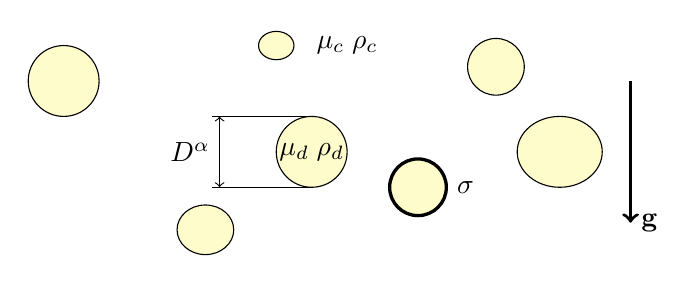
\begin{tikzpicture}[scale = 0.9]
        \draw[fill=yellow!20](3,3) node{$\mu_c\;\rho_c$};
        \foreach \x/\y/\ra/\r in {2/3/0.2/0.25,
        5.1/2.7/0.4/0.4,
        1/0.4/0.35/0.4,
        4/1/0.4/0.4,
        6/1.5/0.5/0.6,
        -1/2.5/0.5/0.5}{
            \draw[fill=yellow!20](\x,\y) ellipse(\r cm and \ra cm);
        }
        \draw[fill=yellow!20](2.5,1.5) circle(0.5)node{$\mu_d\;\rho_d$};
        \draw[thin,-](1.1,2)--++(1.4,0);
        \draw[thin,-](1.1,1)--++(1.4,0);
        \draw[very thick,black!80!black](4,1) ellipse (0.4cm and 0.4cm);
        \draw[very thick,black!80!black](4,1)++(0.4,0)node[right]{$\sigma$};
        \draw[thin,<->](1.2,1)--++(0,1)node[midway,left]{$D^\alpha$};
        \draw[very thick,->](7,2.5)--++(0,-2)node[right]{$\textbf{g}$};
    \end{tikzpicture}
    \caption{Scheme of droplets immersed into a continuous fluid phase.}
    \label{fig:scheme}
\end{figure}

There is a total of $9$ independent physical parameters to this problem (if we consider only the mean of the sizes $D$), they are all constituted by 3 fundamental units, a length, a mass and the time.
Therefore, according to Buckingham $\Pi$ theorem we can define a minimum of $9-3 = 6$ dimensionless numbers to describe the problem. 
Several options are available the selection is somewhat arbitrary, so we choose the following set of dimensionless numbers. 
The $4^{th}$ first parameters are linked to the physical properties of the emulsion, namely, 
\begin{align*}
    & Ga^2 =\frac{\rho_c(\rho_c - \rho_d) g D^3}{\mu^2_c}& 
    & Bo =\frac{(\rho_c - \rho_d) g D^2}{\sigma}&
    & \mu_r = \frac{\mu_c}{\mu_d}& 
    & \rho_r = \frac{\rho_c}{\rho_d}&
\end{align*}
And the two remaining parameters are related to the topology of the flow, 
\begin{align*}
    \phi = \frac{V_d}{V_c} & &
    N_b = \frac{6V_d}{\pi D^3}
\end{align*}
with $N_b$ is the number of droplets in the volume considered and $\phi$ the volume fraction of the dispersed phase.
The \textit{Galileo number} or \textit{Archimedes number}, is the ratio of the buoyancy forces over the viscosity forces, noted $Ga$.
Note that the \textit{Reynolds number}, defined by, $Re = \rho_c L U/\mu$, where $U$ is the characteristic velocity, is equivalent to the \textit{Galileo number} if we take $U = \sqrt{gL(\rho_c-\rho_d)/\rho_c}$ as the velocity scale.
$Bo$ is the \textit{Bond} or \textit{E\"otv\"os number}, it is the ratio between the buoyancy forces and surface tension forces. 
Note that $We = Bo/Ga^2$, with $We$ the \textit{Weber number} compares the viscous forces with capillarity forces.
Thus, $We$ describe the deformation of the droplets, as an example, above a critical value of the \textit{Weber number} a droplet will break due to hydrodynamical forces \citet{deike2022direct}. 
Lastly, $\mu_r$ and $\rho_r$ are respectively the density and viscosity ratios. 

To give a brief idea about the range of interest of those numbers in the industrial context, we take the example of an oil/water emulsion.
In the real processes the diameter of the droplets lies in the range $D = [10 \mu \text{m}, 1 \text{mm}]$.
The density and viscosity of water are approximately $\rho_c = 1000 \text{kg/m}^3$ and $\mu_c = 10^{-3}$.
The density and viscosity of oil are close to $\rho_d = 900 \text{kg/m}^3$ and $\mu_d = 10^{-2}$.
We consider the gravity acceleration on earth, thus it is $g= 9.81 \text{kg.m.s}^{-2}$.
The surface tension of the system oil/water is known to be approximately $\sigma = 50 \text{mJ/m}^2$ \citep{de2015gouttes}. 
We display the values of dimensionless parameters computed with those physical parameters in \ref{tab:parameters}.
\begin{table}[h!]
    \centering
    \caption{Dimensionless parameters for a water/oil emulsion.}
    \begin{tabular}{|c||c|c|c|c|c|}
        \hline&$Ga$&$Bo$&$\phi$&$\mu_r$&$\rho_r$\\ \hline
        \hline Oil/Water&$[0.03,30]$&$[10^{-6};10^{-2}]$&$[0,0.15]$&$0.1$&$1.111$\\ \hline
    \end{tabular}
    \label{tab:parameters}
\end{table}
We can note that the \textit{Galileo number} is rather low therefore can already state that it will be necessary to investigate the stokes flow limit. 
Likewise, The \textit{Bond number} is very low, meaning that the droplets are nearly spherical.
Consequently, in the following models and numerical simulations we must consider some cases with spherical particles. 
The viscosity and density ratio as well as the volume fraction do not permit any additional assumption on the flow. 

\section{Current state of dispersed two phase flow  modeling}

Up to now a lot of investigation have been made on the modelling of bubbly flows.
Indeed, bubbly flows are of a large interest since they appear in plenty application (especially the nuclear industry).
Consequently, researcher have been trying to find closure terms on the specific case of bubbly flows. 
For these reason most of the study cited below investigate bubbles hydrodynamics (and not droplets). 
Also, in the perspective of modeling the reactor scale authors have developed software carrying out Euler-Euler simulations. 
The most famous ones are NEPTUNE-CFD belonging to EDF, and OpenFoam with its collection of multiphase solvers. 
Again, most of the authors carried the computation of the averaged equations of bubbly flows and not emulsion.
Even through in this thesis we solely focus on the closure terms calculation, it is of interest to say a few worlds on the modeling of the upper scale.
i.e. the industrial scale, where we solve the averaged equations derived in \ref{chap:avg}. 

\subsection{Macro scale modeling with CFD-PBM}
Here is a brief review of the authors who attempted to carry out CFD-PBE simulation.
\citet{wang1995simultaneous} study numerically the PBM equations for buoyancy driven setting of spherical drops suspension.
They consider a one dimensional PBE for the axis along the column. 
And solve for the continuous size distribution function $f$.
The source terms $B(n)$ is modeled using the theoretical formulas depicted in the previous chapter, and the probability of coalescence is assumed to be 1 since there is no bouncing in the absence of inertia (therefore a contact results always in coalescence). 
In this context they could  solve the equations, and they show how the coalescence influence the phase separation inside a vessel.
In \cite{KAMP20011363} they solve numerically the averaged PEB considering one dimensional and spherical bubbly flow.
They solve the first and second order equations of the PBE (see \ref{eq:PBM_QBMM3} in \ref{chap:avg}).
They also considered the velocity of the bubbles as independent of the bubble size. 
The coalescence kernel is derived for unequal bubble size interaction in turbulent flows. 
The results are validated with experimental data on pipe flows under microgravity conditions. 
They could show that the coalescence rate diminishes between the inlet and outlet due to the decrease of the rate of collision because the velocities of collision are  higher. 
Next,  \citet{morel2010comparison} performed simulation of Euler-Euler models coupled with PBE for bubbly flow columns. 
They considered 4 different situations with different hypothesis, namely, the single size approach, the moment approach based on the log-normal distribution, the moment approach based on the quadratic law and the multi-fields approach.
The latter method is also called the class method mentioned in the previous chapter (it consists in solving N equation for the mass and momentum for the N class of particles).
They conclude on that from the first to the last method the accuracy increased together with the numerical cost.
Apart from the last method which is completely different from the others and turn out to over predict coalescence. 
Now, in \citet{gemello2018modelling} a full CFD-PBM is modeled for bubbly column on the code \texttt{OpenFoam}. 
The CFD part is modeled with the averaged Navier Stokes equation.
They use classic turbulence model (i.e. $k-\varepsilon$ model, RNG $k-\varepsilon$ and $k-\omega$ model) to account for the velocity fluctuation term, $\left<\bm{u}'\bm{u}'\right>^f$. 
They conclude that $k-\omega$ was the most practical model in terms of accuracy and stability.
\citet{alam2022cfd} conducted CFD-PBM and experimental study on a nano-bubble generator. 
They also compared different turbulence model and found out that the $k-\omega$ model predicted a better prediction for high flows rate.
Note that this modeling of the pseudo turbulent tensor is not physical as pseudo turbulence is different from classic turbulence.
A sightly different work is done by \citet{salehi2017population}, they coupled Large Eddy simulation to PDF-PBM to predict the distribution shape and size of droplets in atomization turbulent flows. 
The dispersed phase is here modeled with a Lagrangian approach, the drag force term use the mean velocity difference between the averaged continuous phase and the dispersed phase.
The additional feature in this work is that they take in account the size and the shape as a variable in the droplet distribution.
The strategy of stokes binding is used here, this method consisting in representing one notional particle for a particle size.

Though, all the processes modeled by these author involve poly disperse two phase flow, none or few of them, considered accurate closure for the velocity fluctuation (they often consider turbulence-like models) and the other the first order closures terms are neglected. 
The reason, is that no accurate closure terms exist yet in the literature. 
Only the drag forces seem to be predicted from robust semi-empirical correlations, for bubbly flow at least.
Besides, of all these authors few of them tried to model gravity induced motion of droplets. 

\subsection{DNS modeling of suspended particles or droplets}

Now, let's focus on the numerical studies providing empirical expression for the closures terms. 
Numerous authors worked on the topic, most of them are already mentioned in \ref{chap:avg} for their theoretical work. 
Note that all the following articles are rather recent since DNS of bubbly flow is quite expensive and is achievable since only a few years. 
\citet{esmaeeli2005direct}carry out  DNS of representative periodic volume of bubbly flow. 
They measure the rising velocity, velocity fluctuation as well as the relative orientation of the pair of bubbles.
Furthermore, they could predict the averaged rising velocity reasonably well, as it is the simplest quantity to predict among all the closure terms.
Indeed, the rising  velocity is the quantity that converge faster than the other thus less sample is needed to predict it.
At the time they were limited by computer performances, thus, the maximum Reynolds number archived is $Re  = 77$, indeed more grid points is needed for higher $Re$. 
They simulated deformable and non-deformable bubbles.
The main difference is that the spherical bubbles form \textit{raft} where the arrangement of the deformable bubbles is pretty random. 
They also found a Gaussian distribution for the velocity fluctuation.
In a more recent work \citet{willen2019resolved} carry out simulation of settling equal spheres in an upward flow.
They also compute the velocity and velocity fluctuation and show that the suspension were anisotropic in the direction of the gravity force.
Besides, they also measure the architecture of the flow and recover the column arrangement and horizontal arrangement, to analyze the structure they used tetrads which allows them to see the evolution of the relative positions.
\citet{du2022analysis} perform DNS calculation of mono disperse bubbly flow and focus on the calculation of pseudo turbulent tensor. 
They separate the pseudo turbulence tensor into two contribution.
The wake induced turbulence and the potential flow and averaged wake fluctuation.
The former is the main focus of the study and a model is proposed.
All these study used DNS and analyze the closure by computing it directly.
But other authors considered wave analysis to get the closure terms. 
We won't go into details, but it is possible to compute several closures by the analysis of the wave speed.
For more information we point the reader to the following articles,  \cite{duru2002constitutive}, \citet{willen2017continuity} and\citet{derksen2007direct}.
On another hands \citet{wang2021numerical} performed DNS of a random array of fixed spherical particle.
About 3000 spheres were modeled to get a representative sample. 
They computed the PFP stress based on the nearest particle statistic reviewed \ref{chap:avg}.
They show that this particle stress can predict the skewing effect along the flow direction and repealing effect on the normal directions of the particular phase. 
This is the only study reporting the calculation of the PFP stress therefore a need is clearly needed on this matter.
\citet{manga1995collective} studied experimentally as well as numerically, with boundary integral methods, the rate of coalescence of interacting pairs of drops.
They investigated the influence of deformation on the rate of coalescence and conclude that greater the drops or bubble deform (for high $Bo$ and  $Ga$) the higher the probability of coalesce will be (might go up to one order of magnitude above than for non-deformable drops).
It also results in a wider distribution of the particles size.
\citet{innocenti2020direct} simulated 3D column of rising bubbles and evaluated velocity fluctuation and energy dissipation for turbulence. 
Interestingly their simulations'  setup is really close to what we wish to accomplish. 


From all those studies presented above it seems that getting the closure terms through DNS seems well achievable.
The most suited set up in our case seems to be the simulation of array of droplets similarly ti \citet{innocenti2020direct}.
Indeed, they could measure the velocity fluctuations properly and other closures like the drag forces (through the averaged velocity) and also terms related to turbulence modeling. 
However, to avoid the modeling of a large domain we will make use of periodic boundary conditions.
This way we will be able to provide closure terms for buoyant driven emulsion.
Besides, all the closure will be calculated simultaneously in one simulation (averaged rise velocity, fluctuation velocity of the fluid and particulate phase\ldots). 
Therefore, in the next section we present the methodology to carry out massive DNS of tri-periodic random array of rising drops.


% \subsubsection{Direct Numerical simulation}
% In order to model film drainage in simulation one has to model all the different length scale from one diameter to $10^{-5}$ diameter. 
% This is technically impossible in a suspension of drops.
% Thus, several technics are available. 
% \citet{thomas2010multiscale} implement theoretically the expression of the flow between the interface of the drop and a wall to avoid refining and solving the layer with DNS.
% This method enable us to the thinning of the film thinner than the length of a cell. 

% \section{Basilisk a suited software to perform massive DNS calculations.}

In view of the previous research (especially the study of \citet{innocenti2020direct}) and the good results obtained in \citet{Naanouh2021numerical}, we thought that the partial differential equation solver, Basilisk (from \url{basilisk.fr}), was the most suited code to carry out tri-periodic simulation of buoyant droplets. 
Originally this code is based on the older code,  \texttt{Gerris}, and was developed primarily by Francesco De Vita, Jose-Maria Fullana, Geoffroy Kirstet-ter, Pierre-Yves Langrée, Emily Lane, Jose Lopez-Herrerra, John MacFarlane, Stéphane Popinet, Clément Robert, and Antoon van Hooft .
Both codes are open source, that is why since then the community contributed to the development of Basilisk and numerous authors published their contribution to the code in scientific reviews.
The open source aspect of Basilisk is somewhat essential for us since it enable us the to develop any desired features.
Besides, a lot of benchmarks demonstrated the good performances and the broad abilities of Basilisk.
All the algorithms are developed in C, if well done this language has the great advantage of optimizing the memory management, resulting in a better computation efficiency. 
Moreover, a lot of physical solvers are already implemented in the code, from wave modeling \citet{mostert2022high} to the simulation of suspended solid particles in a fluid using immersed boundary method \citet{shui2015direct}.
A last feature that has been recently implemented in Basilisk is the multilayer solvers \citep{popinet2020vertically} which will be of great interest in the modeling of film drainage problems. 
We refer the reader to this link \url{http://basilisk.fr/src/README} to see the whole range of possibilities offered by Basilisk.
Nevertheless, the most interesting feature for our use is the capability of modeling two phase flow in Basilisk. 
Indeed, the Volume-Of-Fluid (VOF) method implemented in Basilisk have shown great performance and accuracy, (see \citet{popinet2009accurate}\citet{popinet2018numerical}). 
This point will be developed in a following section since it is of major importance. 
Another practical aspect of Basilisk is that the meshing is included in the workflow of the simulation. 
This enables the possibility of switching between 2D cases and 3D cases automatically, indeed the \textit{dimension} parameter need to be switch from 2 to 3 the rest is automatic. 
In our case it is of a great use since we will start by carrying out 2D simulations and after validation we will switch to 3D mesh.
Speaking of the mesh, Basilisk provide several mesh types that considerably improve the efficiency of the calculation.
The first one is the classic Cartesian mesh, it is fully orthogonal, this is the most for mono-scale problem.
Another interesting grid is the adaptive mesh, as indicate by its name this mesh refines the area where high velocity gradients is observed.
\citet{innocenti2020direct} model a large quantity of bubbles in a container, this was only possible thanks to the adaptive mesh solver, otherwise it would have been too expansive.
The simulation of wave crashes by, \citet{mostert2022high} was made possible also thanks to the adaptive mesh refinement.
Numerous other examples testify of the usefulness of the adaptive mesh refinement solver.   
Then the last meshing technics is a subcase of the adaptive mesh, it is the \texttt{multigrid} mesh, presented in \citet{popinet2003gerris} for the incompressible Euler equations, and more recently in \citet{popinet2015quadtree} for the fully-nonlinear Boussinesq wave equations. 
This meshing technics consist in working with different levels of refined grids simultaneously.
More details will be given about the meshes in this section. 
Finally, the last point on which we would like to emphasize is that Basilisk is a self independent software (i;e. Only the source code of basilisk is needed to compile it) and simulations are launch via C files. 
Which makes it practical for the execution on any machines (cluster or not). 
In the next sections we present the specificity of the VOF methods, needs we speak more specifically about our numerical setup to model rising suspension of droplets. 



\subsection{The Volume Of Fluid Method}

The VOF method is used to model two-phase (or more) flows. 
The governing equations, solved by our solver in the present case, are the one-fluid formulation equation of momentum and mass, presented in \ref{chap:avg}. 
We recall their form here, 
\begin{equation}
    \pddt (\rho \textbf{u})
    = \nablabh \cdot (\textbf{T} -\rho  \textbf{u} \textbf{u})
    + \textbf{b}
    + \textbf{f}_I\delta_I
    \;\;\;\text{and}\;\;\;
    \pddt \rho
    = 
    - \nablabh\cdot(\rho\textbf{u}_k). 
\end{equation}
Note that the material properties (i.e. $\rho$ and $\mu$) takes the value of the phase in presence. 
As seen in \ref{chap:avg}, in two phases flows we define a phase indicator function $\chi$, which is a marker to identify the phases in presence.
When, $\chi = 1$, we are located in the dispersed phase, when $\chi = 0$ in the fluid phase for example, therefore $\chi$ correspond to a Heaviside function. 
However, the Heaviside function is not continuous and derivable everywhere. 
This latter point makes the use of $\chi$ impossible in numerical method.
Therefore, in CFD code, we use an approximation of the Heaviside function, namely the color function $C$. 
Since we want to follow the phases with time,  we need to add the equation of transport of $C$ to complete the system, namely,
\begin{equation}
    \frac{\partial C}{\partial t} + \textbf{u}\cdot\bm{\nabla} C = 0.
    \label{eq:cfunc} 
\end{equation}
At this point several methods are available to define $C$ and to discretize these equations. 

Regardless of the definition of $C$ it is important to say a few words on the discretization of the Navier-Sokes equations which is independent of this choice. 
Basilisk uses the finite volume based method to discretize the governing partial differential equations.
A full review of the finite volume method is made in the book \citet{ferziger2002computational}.
The finite volume method consists in discretizing the whole domain of fluid by finite volume called cells. 
This discretized domain is what we call a mesh. 
In Basilisk we use only orthogonal meshes. 
Which means that the cells of the domain are only squares or cubes.
Nevertheless, as mentioned in introduction there are several specificities among these orthogonal grids.   
\begin{figure}[h!]
    \centering
    \begin{tikzpicture}
        \node (a) at (-0.25\textwidth,0){\includegraphics[height = 0.2575\textwidth]{image/pic/Uniforme.png}};
        \node (b) at (0,0){\includegraphics[height = 0.25\textwidth]{image/pic/non-uniform.png}};
        \node (c) at (0.25\textwidth,0){\includegraphics[height = 0.25\textwidth]{image/pic/adaptativemesh.png}};
        \node (leg) at (a.south){(a)}; 
        \node (leg) at (b.south){(b)}; 
        \node (leg) at (c.south){(c)}; 
    \end{tikzpicture}
    \caption{Different type of orthogonal meshes. (a) uniform mesh, (b) Non-uniform mesh, (c) Adaptive \textit{Quad/Octree} mesh. Reprinted from \citet{mani2021numerical}. }
    \label{fig:meshes}
\end{figure}
The first one is the classic uniform grid depicted \ref{fig:meshes} where all the cells have the same size.
The second one is the non-uniform grid. 
It is useful when the user need to refine a specific area of the mesh, due to high local gradient of the velocity for example.
Then, the last one, is the Adaptive \textit{Quad/Octree} Grids, on which we are to give a bit more details.
It consists in subdividing the cells into $2^2$ cells in two dimension, or in $2^3$ cells in 3 dimension. 
Each cell that have the same size form a group.
All the groups are referred by their respective \textit{levels}. 
The group of level 0 is the one with the larger cells size, actually at this there is only one cell of the size of the domain. 
Then as we look at higher levels the size of the cells decrease. 
Besides, Basilisk offer the possibility of the \textit{Adaptive} option. 
Which means that the cells are subdividing or merging themselves automatically all along the simulation time. 
At the frontier between two levels there is what we called the \textit{resolution boundary}. 
Those boundaries, are somewhat problematic since the cells on each side are not of the same size.
Therefore, the basic operation of the finite volume method are not trivial anymore. 
To avoid this issue Basilisk use \textit{halo cells}.
One \textit{halo cell} is the representation of the cell of the lower level that gather the mean value of the four smaller cells.
The former cell is of the same size of the cell at the other side of the \textit{resolution boundary}, that is why the system is consistent. 
In Basilisk the cells from which the \textit{halo cells} are build are called the children cells, therefore the lower level cells are the parent cells. 
This principle is used for the adaptive mesh, nevertheless, the \textit{Quad/Octree} grid has one subclass, the \textit{multigrid} mesh. 
This meshing technics is no more than a uniform mesh where we make use of the \textit{halo cells}, and parent/children principle. 
Even though there is no \textit{resolution boundary}, this technics allows the user to loop through different levels and through each branch of the mesh. 
This feature is of a great interest to carry out fast operations on vector or scalar fields. 
We refer to the publication of \citet{popinet2015quadtree} for a more detailed explanation.  
Once the mesh is set one need to discretize the governing equations in space and time (see \citet[chapter 3]{tryggvason2011direct}). 

Five main option exist to define the color function $C$ :
the volume of fluid method,
the front taking method,
the level-set method,
the phase-field method
and the CIP method.
As the title of this section is the \textit{volume of fluid method} one could guess which one we use. 
For more details on the other methods we refer the reader to \cite[Chapter 4]{tryggvason2011direct}. 
With the Volume-of-fluid method the color function is now defined by a \textit{VOF tracer}, $f_i$, where $k$ stand for the indices referring to the phase. 
For $N$ VOF tracer $f_k$ is defined for $0\leq k\leq N$.
From $k=0$ for the continuous phase to $k=1$ to $N$ for the dispersed phases (in case we have $N$ dispersed phases). 
In practice the function $f_c$ is not computed since we have the relation, $f_c = 1- \sum_{k=1}^N f_k$. 
The value of the $f_k$ is comprised between $0$ and $1$.
$f_k = 0$ meaning that the concentration of phase $k$ is null, $f_k = 1$ meaning that $100\%$ of the volume is occupied by the phase $k$. 
Note that in every cell the value of $f_k$ is either $0$ or $1$, except in the cells including an interface where the value is the percentage of the phases in presence.
\begin{equation}
    f_k = \left\{\begin{tabular}{cc}
        $1$  &if $\textbf{y}\in V_k$\\
        $0$  &if $\textbf{y}\in V_c$\\
        $0$ to $1$  &if $\textbf{y}\in V_c \cap V_k$\\
    \end{tabular}
    \right.,
\end{equation}
where $V_k$ is the volume occupied by the phase $k$.
The overall condition is that $\sum_k^N f_k \leq 1$.
Next, if we note $\rho_k$ and $\mu_k$ the material property of phase $k$ we can finally compute in each cell the value of the material properties,
\begin{equation*}
    \rho 
    = \sum_k^N \rho_k f_k 
    + (1-\sum_k^Nf_k)\rho_c 
    \;\;\;\text{and}\;\;\;
    \mu 
    = \sum_k^N\mu_k f_k 
    + (1-\sum_k^Nf_k)\mu_c.
\end{equation*} 
In the neighboring cells of the interfaces the calculation of $\rho$ and $\mu$ are slightly different \citep{tryggvason2011direct}. 
Then, once the material properties are calculated, the Navier-Stokes equations solved and the VOF tracers advected, the last step is to reconstruct the interfaces from the $f_k$.
To do so, several methods, more or less accurate, are available  to us.
\ref{fig:VOF} depicts the different reconstruction method, namely, the Simple Line Interface Calculation or SLIC method, the Hirt and Nichols reconstruction method and the Piecewise Linear Interface Calculation or PLIC method. 
As we can clearly see on the scheme the methods goes from coarse (with SLIC) definition of the interface to a more accurate reconstruction (with PLIC).
\begin{figure}
    \centering
    \includegraphics[width = 0.4\textwidth]{image/pic/VOF.png}
    \caption{VOF reconstruction of the solution for advection in two dimensions. 
    (a) The original interface. 
    (b) The original SLIC reconstruction. 
    (c) The Hirt and Nichols reconstruction. 
    (d) PLIC reconstruction. 
    Reprinted from \citet{tryggvason2011direct}.}
    \label{fig:VOF}
\end{figure}
In Basilisk we use PLIC method using height functions (see \citet[Chapter 5]{tryggvason2011direct}). 
Here is a quick summary of how height functions work.
Each segment is parametrized by its normal $\textbf{n}$ and the intercept of a line, $\alpha$. 
Then, in the local reference frame of coordinate $\textbf{z}$, it is possible to define the interface by,
\begin{equation}
    \textbf{n}\cdot\textbf{z} 
    = \alpha,
\end{equation}
where $\alpha$ is computed with the local volume fraction of the phase and the unit normal. 
The overall error is of second order. 
Nevertheless, it must be said that even though the PLIC method is accurate, it still has some draw back sheared with the two other methods. 
Indeed, if we consider 2 tracers the interface is reconstructed considering the tracer $f_c$ and the tracer $f_1$.
Which is equivalent to consider two phases, up to now everything is normal. 
But, consider two interfaces getting closer, then at some point the interfaces will merge together discarding the physical aspect.
Indeed, since we compute height functions from the local volume fraction, if two drops with the same tracer met, then the interfaces are reconstructed regardless of the physical geometry. 
Another problem is that VOF tracers are advected separately so interpenetration of different VOF tracers can happen (this issue will be developed in the next section). 
These two facts mandate the use of a relatively fine mesh so that the film between the droplets is partially resolved.

Once the interface is reconstructed, we can tackle the most challenging problem of VOF simulations.
Which is the modeling of the surface tension forces, i.e. the source term, $\textbf{f}_I\delta_I$, in the one-fluid formulation equations.
Obviously we will not detail the solutions here, to get an overall vision of the problem we refer the reader to \citet{popinet2018numerical} or  \citet[Chapter 7]{tryggvason2011direct}.
However, we can cite the two most basic method.
The first one is the \textit{Continuous surface force method}, in consist in discretizing the expression of the surface force source term. 
Note that the expression of $\delta_S$ make use of the color function, it is in fact equal to the gradient of the color function. 
The approximation of the surface force source term is then,
\begin{equation}
    \sigma \kappa  \textbf{n} \delta_I 
    = \sigma \kappa \nabla f_i,
\end{equation}
where the curvature $\kappa$ is estimated through height function \citep{popinet2018numerical}. 
The other method is the \textit{Continuous surface stress method} which is equivalent, but instead of discretizing the force term, we discretize the divergence of a stress.
It reads, 
\begin{equation}
    \textbf{f}_I \delta_I = \nabla \cdot \left[\sigma (\textbf{I}-\textbf{nn})\delta_I\right],
\end{equation}
\tb{Find were does that came from}
which is valid even with non-constant $\sigma$. 
In Basilisk, we make use of the former method. 

The overall difficulty encountered in the two-phase flows simulations is to manage the singularities at the interfaces.
Indeed, it is a common problem in mathematic when the function is not derivable everywhere.
Hence, from a numerical point of view it is no less of a problem. 
In the conclusion of this chapter we will review some issues arising in  the simulation of emulsion because of this point. 

\subsection{Numerical coalescence}

As briefly mentioned in the preceding section, numerical coalescence can occur during a simulation if two interfaces are one cell mesh apart (assuming there is a solely VOF tracer). 
However, in \ref{chap:avg} we showed that the coalescence of two droplets is a multiscale phenomenon. 
At first, it involves hydrodynamical and lubrication forces.
Once the interfaces are close enough Van deer Waals forces are responsible for the coalescence.
The former forces are well modeled when using a fine enough mesh. 
Indeed, we solve the Navier-Stokes equation together with the transport of the color function, which is the basis of the calculation of the lubrication forces \citep{guazzelli2011}. 
However, the latter contribution involve microscale interaction which are not included in this model.
Even though, it is possible to include Van der Waals forces in Basilisk, it would be too expensive to compute the film drainage problem for several droplets at the same time.
To avoid this problem \citet{thomas2010multiscale} modeled the film drainage by allowing coalescence when the contact time of the droplet is greater than the critical time of contact (computed theoretically).  
However, the closure for the contact time is not well define for our parameters yet.
Moreover, before allowing coalescence after a critical time, we need to prevent it anyway. 
Hence, in any cases we need to prevent coalescence event to happen since DNS of the film drainage is too expansive numerically. 
Besides, to create accurate closures terms seen in \ref{chap:avg}, we need to identify accurately the topology of a given situation.
This way we will be able to give the value of a closure term in terms of the exact number and size of the droplets for example. 
This implies that we must keep a constant number of droplets all along the simulation.

Before avoiding coalescence to happen it is important to identify why it does happen. 
The reason why numerical coalescence occurs is that only one VOF tracer is used. 
Indeed, let's take two drops approaching each other. 
The VOF tracer is advected along the velocity fields. 
We recall that in the interfacial area the VOF tracer has a transitional value between $1$ and $0$. 
Therefore, when the drops eventually get close enough the VOF tracer at the interface of the drops meet each other in the same cells. 
Since the same VOF tracer is used for the two droplet, it results in the addition of the values of the VOF tracer at the interfaces since they gather in the same cells. 
Then, as the VOF tracer merge it is impossible to reconstruct the interface of the respective droplets. 

Using different VOF tracer would prevent the drops to coalesce 
Indeed, during advection the VOF tracer will not sum with the neighboring ones thus the reconstruction of the interface will be possible. 
However, in the literature, we see that we need about hundreds of particles to be able to get a representative volume. 
And since we need to advect each VOF tracers independently, it would be too expensive to have one VOF tracer per drops.    
Luckily, we only need that the adjacent droplets at a given time $t$ have different VOF tracer. 
In 2D the famous \textit{four color map theorems} stipulate that we only need 4 color to color adjacent country with a different color (this is a topological proof).
For our concern, it does mean that we will need no more than four VOF tracer in order for the adjacent droplets to have different VOF tracer. 
In 3D this theorem is not valid anymore. 
Moreover, the droplets move within time thus their neighboring particles changes, and they might need a different VOF tracer.

To tackle this issue \citet{mani2021numerical}, developed an algorithm on Basilisk to carry out the previous task automatically. 
Even though, this algorithm is based on empirical observation and not topological arguments it prevents from using too much VOF tracer. 
The workflow is as follows.
In a first step we identify the VOF tracer having droplets that are close to each other. 
Then for each of these VOF tracers, we identify the pairs of droplets. 
Then we check which of the droplets among one pair have the least neighbors. 
Finally, we switch the VOF tracer of the former droplet to a new tracer that is not in the vicinity of the droplet. 
If no VOF tracer is available then we create a new one. 
In the practical case we indeed notice that 2D simulations do not use more than 4 VOF tracers. 
Therefore, this is a proof of the efficiency of the algorithm. 
This algorithm considers a droplet close to another one only if they have VOF tracers two cells apart.
Consequently, if the drops relative velocity is greater than that this length time the time step then the algorithm will not work.
Nevertheless, in practice the CFL condition is respected which means that the distance traveled by a fluid particle is never superior to one mesh cell. 
This algorithm is launched every time step by default, nevertheless we could call it every 2 time steps (since three would be a bit reckless). 
\tb{more details on this matter }
\subsection{Simulation of periodic rising droplets}
As concluded in the two previous sections, we are going to make DNS of a random array of droplet rising in a continuous Newtonian fluid with the code Basilisk. 
Therefore, in this section we are going to present the 


In Basilisk the computational domain of the simulation must be a square in 2D or a cube in 3D, as depicted on \ref{fig:numscheme}. 
Depending on the desired number of bubbles $N_b$ we divide the domain of size $\mathcal{L}$ in $N$ smaller squares of length $\Delta$.
In each smaller squares we initialize the VOF tracers $f_i$ as a spherical, in 3D, or circular, in 2D, shaped area representing the droplets.
Each droplet of diameter $L$ is centered inside their $\Delta\times \Delta$ square.
Besides, we add a random shift vector for each droplet position so that all the simulations with the same parameters are unique. 
The shift must be limited in order to avoid that the drops touch each other at the initialization time (in which case they would immediately merge).   
Also, another method consist of initializing all droplets randomly, making sure that they are initially far enough so that they do not touch each other at the first step of the simulation.
The latter technics was used in the simulation performed in \ref{chap:mono-disperse} since it has shown faster convergence. 
Indeed, as we initialize with a random state, the suspension takes a shorter amount of time to reach it statistically random steady state. 
\begin{figure}[h!]
    \centering
    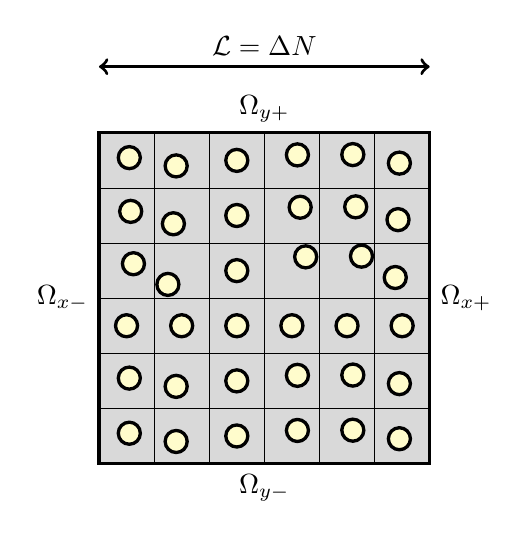
\begin{tikzpicture}[very thick,scale = 0.7]
        \draw[fill=gray!30](0,0) rectangle(6,6);
        \foreach \x/\dx in {0.5/0.1,1.5/-0.2,2.5/0,3.5/0.2,4.5/0.21,5.5/-0.1}{
            \draw[very thin](\x+0.5,0)--(\x+0.5,6);
            \draw[very thin](0,\x+0.5)--(6,\x+0.5);
            \foreach \y/\dy in {0.5/0.1,1.5/+0.1,2.5/0,3.5/0.25,4.5/0.15,5.5/0.1}{
                \draw[fill=yellow!20](\x+\dx*\dy*5,\y+\dy*\dx*5) ellipse(0.2 cm and 0.2 cm);
            }
        }
        \draw[<->](0,7.2)--(6,7.2)node[midway, above]{$\mathcal{L} = \Delta N$};
        \draw(3,6)node[above]{$\Omega_{y+}$};
        \draw(3,0)node[below]{$\Omega_{y-}$};
        \draw(6,3)node[right]{$\Omega_{x+}$};
        \draw(0,3)node[left]{$\Omega_{x-}$};
    \end{tikzpicture}
    \includegraphics[width=0.45\textwidth]{image/3D/PHI01.png}
    \caption{(left) Scheme of the initialization of an array of droplets immersed in a 2D periodic domain.
    (right) Picture of a 3D simulation with $\phi = 0.1$, $N = 5$ the color represent the velocity field.}
    \label{fig:numscheme}
\end{figure}

The dimensionless parameters of this study have been already discussed in \ref{chap:avg}.
Nevertheless, additional dimensionless parameters must be introduced since numerical parameters that weren't on the theoretical problem appear. 
Only six parameters are needed among the existing dimensionless parameters. 
However, the numerical simulations involve an others length parameters among the ones already mentioned in \ref{sec:introavg}, namely the length of a cell in the mesh.
Therefore, we need to define a new dimensionless parameter, namely, the number of cells per diameter refer by $\delta$. 
From those parameters it is possible to recover the physical parameters needed by the simulation. 
But before we fix the following parameters, $\rho_d = L = g = 1$ for convenience.
Then it yields the following relations to recover the remaining parameters,
\begin{align*}
    &\rho_c = \rho_d\rho_r ,&
    &\mu_d  =\frac{\rho_d \sqrt{|1-\rho_r| \rho_r g \bar{L}^3}}{\mu_r Ga},&
    &\mu_c  = \mu_d\mu_r,&
    &\delta  = D/Nc& \\
    &\sigma = \frac{|1-\rho_r|\rho_d g L^2}{Bo},&
    &\Delta = \sqrt{\frac{\pi D^2}{4\phi}},&
    &\mathcal{L} = \Delta \sqrt{N_b}.&
\end{align*}
From those parameters it is possible to define different time, length and velocity scales. 
It will be useful when we will need to make the results dimensionless. 
The different scales in which we will be interested in are the following.
\begin{align*}
    &U_\mu = \frac{g D^2 \Delta \rho}{\mu_c}&
    &U_\rho = \sqrt{\Delta \rho \frac{Dg}{\rho_d}}&
    &U_\sigma = \sqrt{\Delta \rho \frac{Dg}{\rho_d}}& \\
    &T_\mu = \frac{\mu_c}{g\Delta \rho D}&
    &T_\rho = \sqrt{\frac{\rho_dD}{g\Delta\rho}}&
    &T_\sigma = \sqrt{\frac{\rho_{avg} D^3}{\pi \sigma}}&
\end{align*}
Were $U_\mu$, $U_\rho$ and $U_\sigma$ are respectively the viscous inertial and capillary velocity scales. 
Similarly, $T_\mu$, $T_\rho$ and $T_\sigma$ are the corresponding time scales. 
Here is a quick explanation of the physical meaning of those scales :
When $Ga \ll 1$, in one unit of $T_\mu$ a droplet travel a distance of $D$ relatively to the fluid.  
Similarly, When $Ga \gg 1$ a droplet travel a distance of $D$ in one unit of $T_\rho$. 
Lastly, the Capillary time $T_\sigma$ will be the period of one undulation of the surface droplet. 
Of course this scale provide us with an order of magnitude, they aren't exact. 

In Basilisk the set-up of a simulation (solvers and parameters) is made by including or excluding header files.
All the header files can of course be found in the sources of the code (\url{http://basilisk.fr/src/}).   
In the following, we describe the header files used in this simulation. 
The first one has in fact already been mentioned, it is \href{http://basilisk.fr/src/grid/multigrid.h}{multigrid.h} or  \href{http://basilisk.fr/src/grid/multigrid3D.h}{multigrid3D.h} file for 3D simulations. 
It set up a uniform staggered multigrid mesh. 
Then, we add the file \href{http://basilisk.fr/src/navier-stokes/centered.h}{centered.h} to resolve Navier Stokes equation on this mesh with centered formulation.
The \texttt{two-phase.h} header set up the VOF tracers and interfaces for two immiscible fluid.
It also set add transport equation of the VOF tracers coupled with the Navier Stokes solver.
To account for the tension surface forces mentioned in the previous section we include the \href{http://basilisk.fr/src/tension.h}{tension.h} header file. 
This file takes in account the curvature calculation of the interface and the interfacial forces. 
We then add the \href{http://basilisk.fr/sandbox/fintzin/Rising-Suspension/no-coalescence.h}{no-coalescence.h} header which create several VOF tracers depending on the needs in order to avoid coalescence. 
Finally, the \href{http://basilisk.fr/src/view.h}{view.h} and \href{http://basilisk.fr/src/output.h}{output.h} header are included manage the graphical output.  

As mentioned earlier  the boundaries of the domain are periodic. 
It signifies that the velocity field follow the these conditions,
\begin{align}
    \bm{u}(y_i = 0,t) = \bm{u}(y_i = \mathcal{L},t) \;\;\; &\forall \bm{y} \in \Omega_{y_i-} \;\;\;\text{and}\;\;\; \forall i \in \left\{1,2,3\right\}.\\
    \bm{u}(y_i = \mathcal{L},t) = \bm{u}(y_i = 0,t) \;\;\; & \forall \bm{y} \in \Omega_{y_i+} \;\;\;\text{and}\;\;\; \forall i \in \left\{1,2,3\right\}.
\end{align}
And the pressure fields respect similar conditions, 
\begin{align}
    p(y_i = 0,t) = p(y_i = \mathcal{L},t) \;\;\; &\forall \bm{y} \in \Omega_{y_i-} \;\;\;\text{and}\;\;\; \forall i \in \left\{1,2,3\right\}.\\
    p(y_i = \mathcal{L},t) = p(y_i = 0,t) \;\;\; & \forall \bm{y} \in \Omega_{y_i+} \;\;\;\text{and}\;\;\; \forall i \in \left\{1,2,3\right\}.
\end{align}
The advantage of using periodic domain is that we can run the simulations for an arbitrary long times since the droplets loop inside the domain.
Besides, it lets the flow develop freely, which is more physical for representative volume. 
However, it has some drawback.
The first  one is that the physical phenomenons that have a wavelength larger than the domain won't be represented. 
Therefore, the domain still needs to be large enough to represent the desired phenomenons.
And the other one is that, if we were to model the problem as it is, we would see both phases falling though a Cartesian multigrid mesh. 
Indeed, we apply an acceleration $g$ on the whole domain. 
And since our domain is periodic the velocity field will keep accelerating through the infinite domain.
If we discard the numerical issues this is not a problem.
Indeed, we could still measure the relative velocities and fluctuation over the domain. 
But, the thing is that we can not discard the numerical issues. 
Therefore, we set the simulation in the referential of the fluid phase by applying an acceleration $\bm{a}$ on the whole domain equivalent to a null averaged force.
Namely, 
\begin{equation}
    \textbf{a} = - \left[1-\frac{\left<\rho\right>}{\rho}\right]\textbf{g},
\end{equation}
where we use the volume average operator defined in \ref{chap:avg}.
We can notice that the contribution of the force on the whole numerical domain is null.
Indeed, it yields, 
\begin{equation}
   \int \rho\textbf{a} g(\textbf{x,y}) dV 
    = \textbf{g}\int \rho g(\textbf{x,y}) dV -\textbf{g}\left<\rho\right>\int g(\textbf{x,y}) dV 
    =0,
\end{equation}
where we recognized in the last equation the volume average of the density $\rho$.
Now, the net averaged velocity of the domain will be in null in both direction.
Besides, by applying a constant acceleration through the domain we preserved the relative motion.
However, it turns out that this last fact ins't true in practice. 
Indeed, numerical error accumulation of the momentum at the interfaces occurs due to the inconsistency of the numerical schemes (see \citet{popinet2018numerical}).
Besides, due to the discontinuity at the interfaces solvers can either conserve the momentum or the velocity depending on the numerical schemes used.
In our case we conserve the velocity and not the momentum. 
In Basilisk C we could use the \href{http://basilisk.fr/src/navier-stokes/conserving.h}{conserving.h} solver.
Anyhow, as this problem come from different source it is rather difficult to solve it properly.
As an example in the CFD-DEM code \href{https://hal.archives-ouvertes.fr/hal-02170320}{PeliGRIFF}
they directly force a null velocity fields inside the solver steps. 
As this solution is rather sophisticated we choose for another option. 
Indeed, to solve this problem we add an artificial acceleration on the whole domain at each time step. 
If $U_\epsilon$ is the bulk velocity (which should be theoretically null), then the acceleration to cancel this velocity must be equal to $U_\epsilon/\Delta t$ where $\Delta t$ is the current time step. 
In the next pages we will refer this artificial acceleration as the \textit{momentum correction}. 


% 
\section{Validation of the model}

The numerical parameters introduced in the previous section, i.e. the definition of the mesh $\delta$, and the number of droplet per domain $N$ or $N_b$ (see the definition in the previous section) need to be verified. 
Indeed, in view of carrying a numerous amount of simulations it is important to identify the minimum necessary number of droplets per domain and definition of the mesh.
Clearly, if we keep the parameter $\phi$ fixed a larger number of droplets implies a larger domain, therefore a greater numerical cost.  
Besides, the range of physical parameters needed to obtain representative closure need to be investigated to. 
Therefore, in this section we identify the ranges of numerical and physical parameters in order to obtain an efficient framework. 
The validations are all based on parameter independence arguments, meaning that we keep track of a quantity, and validate our model until the quantity is independent of the parameter. 


\tb{\subsection{Comparison with experimental or numerical simulations}
\subsubsection{Comparaison with o rdered array \citet{loisy2017buoyancy} \citep{innocenti2020direct} }
Include and launch simulations with the model of trygvason for buubles 
}
\subsection{Momentum correction}
But firstly, let's validate our last hypothesis, i.e. the \textit{momentum correction}. 
The procedure is the following, we carried out two similar simulations, one with the \textit{momentum correction} referred as the simulation $C1$, and the other without referred as $C0$.
The aim is to compare the values of the closures terms in both simulations and see if there are any differences between $C1$ and $C0$. 
They both have the following dimensionless parameters : 
$Bo = 1$, $Ga = 75$, $\mu_r  =1$, $\rho_r = 1$, $N = 5$ and $\phi = 0.15$. 
In addition, we select a number of cells per diameter $\delta = 15$ so that we intentionally create numerical error (in order to test at the limit of definition our modeling).
Also, both simulations were carried in 3 dimension. 
Of course, we expect no difference between those cases. 
\begin{figure}[h!]
    \centering
    \includegraphics[height= 0.3\textwidth]{image/VALIDATION/C0C1/Ud.pdf}
    \includegraphics[height= 0.3\textwidth]{image/VALIDATION/C0C1/DeltaU.pdf}
    \caption{(left) Absolute averaged velocity of the dispersed phase along the vertical axis.
            (right) Relative velocity between the dispersed and continuous phases.
            (Dashed lines) simulation $C0$,
            (solid lines) simulation $C1$.  }
    \label{fig:VALIDATION_C0C1_1}
\end{figure}
On \ref{fig:VALIDATION_C0C1_1} we can observe the results of the two cases $C0$ and $C1$.
The (left) picture clearly shows that there is a velocity shift when no correction is applied.
Nevertheless, the two cases exhibit the same interphase velocity (see \ref{fig:VALIDATION_C0C1_1} (right)), which results in a same interphase drag force. 
The phase velocity is a term of first order, therefore it is no sensitive to the numerical parameters (e.g, number of drops per domain, number of cells per diameters).
Therefore, it is interesting to observe on \ref{fig:VALIDATION_C0C1_2}, that the similarities still holds on the first order closure terms. 
\begin{figure}[h!]
    \centering
    \includegraphics[height= 0.3\textwidth]{image/VALIDATION/C0C1/UpUpf.pdf}
    \includegraphics[height= 0.3\textwidth]{image/VALIDATION/C0C1/PA_Mh.pdf}
    \caption{(left) Fluids phase averaged fluctuation tensor.
            (right) Particular average of the first moment tensor, where $F_g$ is the buoyancy force applied on one droplet.
            (Dashed lines) simulation $C0$,
            (solid lines) simulation $C1$.  }
    \label{fig:VALIDATION_C0C1_2}
\end{figure}
Indeed, as we can remark the velocity fluctuations and the first moment are quite the same for both simulations.
It is not presented here, but all quantities remain the same thus the \textit{momentum corrector} isn't influencing any of these closures terms. 

\subsection{Number of particles per domain and definition of the mesh}

Now, let's investigate the required number of droplets per domain, $N_b$, and the minimum definition of cells per diameter of droplets $\delta$.  
\tb{Include bibliography and expectation here \ldots}
For this investigation we kept the physical parameters presented in the same section and made a double parametric analysis over $N$ and $\delta$. 
We carried out simulations for $N = 2, 3, 4, 5, 6, 7$, and for a number of cells $10 <\delta < 40$. 
In Basilisk the mesh definition is defined by a power of two, consequently depending on the size of the domain (which is fixed to keep a $\phi$ constant) the $\delta$ parameter is fixed at a power of 2 close. 
\begin{figure}[h!]
    \centering
    \includegraphics[height= 0.3\textwidth]{image/VALIDATION/N_and_delta/DUd.pdf}
    \includegraphics[height= 0.3\textwidth]{image/VALIDATION/N_and_delta/PHI.pdf}
    \caption{(left) Averaged relative velocities for both phases.
            (right) Dispersed phase volume fraction at the end of each simulation.
            The text on the side of the points is $\delta$. }
    \label{fig:VALIDATION_Nd_1}
\end{figure}
\ref{fig:VALIDATION_Nd_1}(left), illustrate clearly that the drift velocity is independent of the parameters $N_b$ and $\delta$, for $N >4$. 
On the other hand, \ref{fig:VALIDATION_Nd_1}(right), show that the volume fraction of the dispersed phase is lower for the low defined grid (red dots), due to a loss of volume during the simulation.
This doesn't mean that the solver isn't volume conservative. 
In fact, it is fund to be due to the \href{http://basilisk.fr/sandbox/fintzin/Rising-Suspension/no-coalescence.h}{no-coalescence.h} which generate fragment into the numerical domain, fragment which are deleted in the long run. 
\begin{figure}[h!]
    \centering
    \includegraphics[height= 0.3\textwidth]{image/VALIDATION/N_and_delta/PA_UpUp.pdf}
    \includegraphics[height= 0.3\textwidth]{image/VALIDATION/N_and_delta/Mh.pdf}
    \caption{(left) Fluids phase averaged fluctuation tensor.
            (right) Particular average of the first moment tensor, where $F_g$ is the buoyancy force applied on one droplet. 
            The numerical values displayed alongside the dots are the number of cells per diameter.}
    \label{fig:VALIDATION_Nd_2}
\end{figure}
Now, let's look at the behavior of more \textit{complicated} closure terms. 
\ref{fig:VALIDATION_Nd_2}(left) demonstrate that the vertical component of the pseudo turbulent tensor is parameter independent rather early, independently of the grid definition. 
This fact is rather surprising but notice that the standard deviation is quite high for small domain. 
On \ref{fig:VALIDATION_Nd_2}(right), we can examine the vertical component of the first moment closure term. 
It is found to be constant for all $N$, but rather inaccurate for coarse grids. 
Which makes sens since the first moment results from a local calculation of the stress over a droplet volume, unlike the other quantities which results from the averaged center of mass velocity of a droplet. 

As we have shown, the quantities presented converge for a number of droplets equivalent to $N = 4$ and $\delta = 25$. 
Thus, we validate our simulation in space, i.e. we made sure that our domain were wide enough to minimize the influence of the periodicity on our results, and in mesh definition. 
Nevertheless, at it is the number of realization that matter when carrying a particular average, it is interesting to look at the duration of the simulation.

\subsection{Time average convergence}

The aim of this study is to be able to identify the minimum required time (or number of time steps) to obtain a representative mean. 
In this set of results we made sure that all the simulations were carried for a time that is more than sufficient. 
Therefore, in this section, we observe the convergence of the mean of a quantity depending on the number of the sample of time taken through the simulation.
More specifically we define the cumulative mean of an already, space averaged quantity, $F$, as, 
$\bar{F}(t) = \int_{T_{start}}^{t} F dt$. 
Where we introduced the start of sampling time $T_{start}$, which correspond to the starting time at which we are gathering data. 
This time is chosen as the time it takes for the simulation to reach a statistically steady state.
In other worlds, it is the time it takes for the droplets to get from an inert ordered state ($t = 0$), to a fully random state, where the droplets reach their mean drifting velocity.
As, we could remark, from its high standard deviation, the most difficult quantity, difficult in the meaning that it doesn't converge rapidly, is the \textit{Reynolds} stress tensor averaged on the particular phase, namely $\pnavg{u'_yu'_y}$.
Thus, we will confirm the representativity of our simulations, by looking at the cumulative time average of this quantity. 
\begin{figure}
    \centering
    % \includegraphics[height = 0.3 \textwidth]{image/VALIDATION/time/Sigma.pdf}
    \includegraphics[height = 0.3 \textwidth]{image/VALIDATION/time/UpUp.pdf}
    \caption{Cumulative mean of the \textit{Reynolds} stress tensor. For $N = 3,4,5$ and $\delta = 25$, with $t/T_{start} = 10$.}
    \label{fig:VALIDATION_cumul_mean}
\end{figure}
From, \ref{fig:VALIDATION_cumul_mean}, it is apparent that the case where, $N=5$, has a faster convergent mean. 
Indeed, if we examine the picture, it is evident that the curve for $N=5$ reach a steady state earlier than the other ones. 
As a matter of fact, it can be perceived that the $N=5$ simulation reaches a steady mean at $t/T_\rho = 25$, while the other converge much latter. 
As a result, this study show, without surprise, that the result of the particular \textit{Reynolds} stress tends toward a steady mean faster for the simulation where $N=5$. 
In view of this it is interesting that for this range of \textit{Galileo} the time required to have significant results it $t/T_{\rho} \approx 110$, where we added the start time and $100$ inertial sampling time. 


\subsection{Asymptotic regime in low \textit{Galileo}}

Ideally we would like to cover a wide range of \textit{Galileo} numbers. 
Meaning that we need to reach both asymptotic regime, at low and high $Ga$ for any closure, if we suppose that such asymptotic regime exist. 
We limit our validation to the drag force or drift velocity closure term. 
In this section we show that in the limited range studied, i.e. $Ge \in [5,100]$, we cover enough \textit{Galileo} number to reach the low and high inertia asymptotic regime. 

First, it is interesting to see that the range of \textit{Galileo} number studied correspond to a wider range of \textit{Reynolds} numbers. 
Indeed, \ref{fig:Ga_Re} we clearly see that the computed \textit{Reynolds} numbers, based on the drift velocity, i.e. $Re = D (\cavg{\textbf{u}} - \davg{\textbf{u}}) \rho_f/\mu_f$, results in a wider range than the input \textit{Galileo} numbers. 
\begin{figure}[h!]
    \centering
    \includegraphics[height= 0.3\textwidth]{image/Dim_3/fCA/Re.pdf}
    \caption{\textit{Reynolds} number computed with the drift velocity, in terms of the \textit{Galileo} numbers.}
    \label{fig:Ga_Re}
\end{figure}
Thus, we cover both regime, inertial for $Re \approx 0.1$ and non-inertial with $Re \approx 100$. 
In order to investigate the different asymptotic regime of the drag force closure term, we plotted, in \ref{fig:f_u_f_rho}, the dimensionless drag force under two different form. 
In the first case (\ref{fig:f_u_f_rho}(left)) it is made dimensionless by the viscous material terms, namely,
\begin{equation*}
    \cavg{\textbf{f}^\mu} = \frac{\textbf{g} D^2\Delta \rho}{\mu_f |\cavg{\textbf{u}} - \davg{\textbf{u}}|}. 
\end{equation*} 
While in the other case it is made dimensionless with the inertial assumption, 
\begin{equation*}
    \cavg{\textbf{f}^\rho} = \frac{\textbf{g} D\Delta \rho}{\rho_f |\cavg{\textbf{u}} - \davg{\textbf{u}}|^2}. 
\end{equation*} 
\begin{figure}[h!]
    \centering
    \includegraphics[height= 0.3\textwidth]{image/Dim_3/fCA/FH_Re_mu.pdf}
    \includegraphics[height= 0.3\textwidth]{image/Dim_3/fCA/FH_rho_Re.pdf}
    \caption{(left) Non-inertial dimensionless vertical drag force term. 
             (right) Inertial dimensionless vertical drag force term. }
    \label{fig:f_u_f_rho}
\end{figure}
In \ref{fig:f_u_f_rho}(left) we can observe that $\cavg{\textbf{f}_\mu^*}$ tend to a constant value for approximately, $Re \le 1$, corresponding to a $Ga \le 5$.
Meaning, that we reach an asymptotic regime at $Ga=5$, and that it will probably tend to this same value at even lower $Re$ or $Ga$. 
However, as demonstrated by \ref{fig:f_u_f_rho} (right) the high inertial regime do not tend to a constant yet. 
Thus, no additional conclusion can be drawn so far for high inertial regime. 

In conclusion, in order to cover a wide enough range of \textit{Galileo}, we do not need to investigate $Ga<5$ since the lower \textit{Galileo} simulations, seems to behave proportionally to the case where $Ga = 5$. 
Regarding the high inertial regime, as we cannot really go above $Ga =100$ (due to the required mesh definition at higher $Ga$), we limit our study to $Ga =100$.  
Consequently, in the following simulation were carried though the range $Ga = [5,100]$, corresponding to $Re \in [1,100]$. 

\subsection{Statistical convergence}

\subsubsection{Pair PDF of presence}

In the next chapter we will see that the radial distribution function has a major importance in the closure problem. 
In order to be representative while reconstructing this function numerically, we need to gather enough sample of relative event of pairs of particles position. 
Thus, when $N$ increase, the number of particles realization of pairs of particles increase, thus we expect that $g(r)$ tends toward a constant function with increasing $N$. 
The question is, how many droplets per domain do we need so that this function is indeed representative (keeping the simulation time and time step constant) ? 
\begin{figure}[h!]
    \centering
    \includegraphics[height= 0.3\textwidth]{image/VALIDATION/fDist/g_r.pdf}
    \includegraphics[height= 0.3\textwidth]{image/VALIDATION/fDist/N_g_1.pdf}
    \caption{(left) Plot of the radial distribution function $g(r)$ for different $N$. 
             (right) Plot of the values of $g$ for $r =1$ in terms of the number of droplets inside the domain for different mesh definition. }
    \label{fig:g_r}
\end{figure}
On \ref{fig:g_r} (left), we see that the radial distribution function $g(r)$, tends to one with increasing $r$, which is exactly what we expect from a radial distribution function, thus it is a first validation. 
Moreover, the value of the radial distribution at $r\approx1$, is of a major importance since it is used in a closure models for the particular phase averaged stress in solid particle suspensions \citep{jackson2000dynamics}, it is also used in kinetic theory for the collision kernel modeling, \citep{fede2015monte}.
Therefore, \ref{fig:g_r} (right) we plotted the value of $g(r=1)$ for different mesh definition and number of particles per domain. 
It is evident that $g(1)$ reach a constant value above $N=4$ for a mesh definition $\delta = 25$. 

We established that the statistical distribution converged radially. 
Nevertheless, we would like to study the angular distribution in addition to the radial distribution.  
Thus, on \ref{fig:VALIDATION_fDrop_3} we show different 2D plots of this 2D distribution function. 
By comparing both plot it clearly indicates that this 2 dimensional distribution converge at $N=5$. 
\begin{figure}[h!]
    \centering
    % \includegraphics[height= 0.35\textwidth]{image/VALIDATION/fDrop/D_nbr_Theta_ndc_10_N_2.pdf}
    \includegraphics[height= 0.3\textwidth]{image/VALIDATION/fDrop/U_Theta_ndc_25_N_4.pdf}
    \includegraphics[height= 0.3\textwidth]{image/VALIDATION/fDrop/U_Theta_ndc_25_N_5.pdf}
    \includegraphics[height= 0.3\textwidth]{image/VALIDATION/fDrop/U_Theta_ndc_10_N_6.pdf}
    % \includegraphics[height= 0.35\textwidth]{image/VALIDATION/fDrop/Dmin_Theta_Ur_uT_75_PHI_0_15.pdf}
    \caption{Radial distribution function of the nearest particle, $P(\theta, D_{nst}/D)$. 
    From $N=4$ (left) to $N=6$ simulations (right).}
    \label{fig:VALIDATION_fDrop_3}
\end{figure}
Indeed, if we look to the color bar of each plot and to the plot itself, we clearly see that the value of the PDF is the same for all $N$. 
Nevertheless, we can distinguish a small difference between $N=4$ and the others, even though it is small it deserves to be notified. 
Therefore, we consider a 2D distribution independence above a number of 64 ($N=4$) droplets per domain. 


\subsubsection{Influence of the mesh definition on nearest statistics}

Now that the required number of sample is fixed need to check out the influence of the mesh definition at the inter particle scale. 

To do so we propose to study the following a case with the following dimensionless numbers. 
We set $Ga = 75$ to be in the most disadvantageous situation. 
\begin{align}
    Ga = 75
    & \phi = 0.1
    & \mu_r =0.1 
    & \rho_r = 1.1
    & Bo = 1 
\end{align}
Finlay we test three number of cells quality, $\delta > 10$, $\delta > 25$, $\delta > 35$. 


\section{Experimental design}

From the previous few sections, we were able to identify and select relevant dimensionless parameters 
to be studied in the next chapters. 
They were deduced from parameters independence depicted in the previous few sections.
They are summaries in \ref{tab:parameters2}.
\begin{table}
    \caption{Ranges of the studied dimensionless parameters.}
    \centering
    \begin{tabular}{|c|c|c|c|c|c|c|} \hline
        $Ga$ &
        $\phi$ & 
        $Bo$ &
        $\rho_r$ &
        $\mu_r$ &
        $T_{max}/T_g$ &
        $\Delta t/T_{\sigma}$\\ \hline
        5-100
        &0.01-0.15
        & 1 
        & 1.1
        & 0.1-10
        & 500
        & 10 \\\hline
    \end{tabular}
    \label{tab:parameters2}
\end{table}
Most of the parameters have been discussed above. 
Regarding, $\phi$ we limited our study below $0.15$ because above this value bubbles or droplets instantaneously coalesce and the flow isn't dispersed anymore. 
Below $\phi =0.01$ the required domain is too wide, thus the simulations would be too expensive to carry, even though lower volume fraction would have been of interest. 
The \textit{Bond} number has been determined based on the shape of the particles. 
Indeed, we know that for extremely low $Bo$ a droplet will remain spherical. 
Thus, as for our application (see introduction of \ref{chap:avg}) we aim for spherical droplets, i.e. \textit{Bond} numbers, we need to seek for convergence toward low $Bo$. 
And as it will be shown in the results, for $Bo =1$, and this range of $Ga$, the particles remain spherical, thus we reach this asymptotic regime for low $Bo$. 
The density ratio $\rho_r = 1.1$ correspond to the ratio of our application. 
Regarding, the viscosity ratio our application (oil /water) is at $\mu_r=0.1$, but we allow our selves to explore a wider range event though we won't be able to describe entirely this dimension. 
The time of the simulation is scaled on the inertial time, $T_\rho$, as the simulations are mostly driven by inertial effect (i.e. $Ga \in [5,100]$). 
The value of $500$ inertial time has been validated empirically as can be shown by the accuracy of the previous results. 
The time step has been scaled with the capillary time in order to sample several time steps in a period of deformation of a droplet. 

In brief, the numerical parameters together with the physical ones are well validated.
Therefore, in the following chapters we carry out simulations in the restricted ranges of the parameters depicted \ref{tab:parameters2}.


\section{Numerical methodology}
\label{sec:methodo}



\subsection{Problem statement}
% Objective of this section :
% \begin{itemize}
    % \item Introduce the dimensionless parameters.
    % \item Present the physical parameters of some industrial processes to locate our problematic. 
    % \item Introduce the dimensionless parameters range investigated in this study.
    % \item Present the tri-periodic box within which we add droplets in vof 
% \end{itemize}
We investigate numerically the dynamic of homogeneous mono-disperse emulsion subject to buoyancy forces in a fully periodic domain. 
Both, the dispersed (resp. continuous) phase is considered as Newtonian fluid defined by viscosity $\mu_d$ (resp. $\mu_f$), and density $\rho_d$ (resp. $\mu_f$).
Throughout this work, the subscript $_d$ and $_f$ indicate properties belonging to the dispersed and continuous phase, respectively. 
The interface between both fluids is considered as infinitely thin and deprived of any impurities, it is described with the surface tension coefficient $\gamma$. 
In this work the density, viscosity, and surface tension coefficient, will be considered constant in each phase.
In dimensionless form this problem is completely characterized by $6$ dimensionless parameters :  the viscosity and density ratio, $\lambda = \mu_d / \mu_f$ and $\zeta = \rho_d / \rho_f$,  
the \textit{Galileo} number, 
\begin{equation*}
    Ga =\sqrt{\rho_f(\rho_f - \rho_d) g d^3} / \mu_f,
\end{equation*}
the \textit{Bond} number, 
\begin{equation*}
    Bo =\frac{(\rho_f - \rho_d) g d^2}{\gamma},
\end{equation*}
the number of droplets per domain $N_b$, and the dispersed phase volume fraction $\phi$. 
Here, $d$ represents the diameter of a sphere with the same volume as the droplets, and $g$ denotes the gravitational acceleration.
The \textit{Galileo} number measure the influence of the buoyancy forces against the viscous forces.
Whereas the \textit{Bond} number evaluate the ratio between buoyancy and capillary forces. 
% These parameters are the input parameters that we set at the beginning of a simulation

To provide a brief overview of the range of interest for these numbers in an industrial context, let's consider the example of a vegetable oil/water system.
In most liquid-liquid system encountered in industrial processes the diameter of the droplets lies in the range $d = [50 \mu \text{m}, 3 \text{mm}]$.
The density and viscosity of water are approximately $\rho_f = 1000 \text{kg/m}^3$ and $\mu_f = 10^{-3} \text{Pa.s}$, respectively.
The density and viscosity of oil are close to $\rho_d = 900 \text{kg/m}^3$ and $\mu_d = 10^{-2} \text{Pa.s}$, respectively.
We consider the gravitational acceleration on earth, thus $g= 9.81 \text{m.s}^{-2}$.
The surface tension of the oil/water system is approximately $\sigma = 0.05 \text{N/m}^2$ \citep{de2015gouttes}. 
% \tb{mettre un fluid arbitraire a la place de lhuile ? je ne vois pas trop comment introduire le pbl dans ce cas}
\begin{table}[h!]
    \centering
    \caption{Dimensionless parameters of a water/oil system.}
    \begin{tabular}{|c||c|c|c|c|c|}
        \hline&$Ga$&$Bo$&$\phi$&$\lambda$&$\zeta$\\ \hline
        \hline Oil/Water&$[0.35,160]$&$[10^{-5};10^{-1}]$&$<0.2$&$10$&$0.9$\\ \hline
    \end{tabular}
    \label{tab:parameters_exp}
\end{table}
In \ref{tab:parameters_exp} we can observe the values of the corresponding dimensionless parameters.  
Notice that the \textit{Bond number} is relatively low, indicating that the droplets are nearly spherical in these processes.
Additionally, the maximum volume fraction is set to $\phi = 0.2$, indeed above such $\phi$ particles highly coalesce and the topology of the flow cannot be considered as dispersed anymore. 


According to \ref{tab:parameters_exp}, to approach real life applications we conducted DNS for four volume fractions, specifically $\phi = 0.01,0.05,0.1,0.2$.
In contrast to most of the previous studies, we choose to keep the number of droplets constant while changing the volume fraction $\phi$. 
Instead, we modify the domain size $\mathcal{L}$ accordingly. 
This introduces another dimensionless parameter of interest : $\mathcal{L}/d$, which is the confinement of the particles within the finite numerical domain. 
This parameter is purely determined by $\phi$ and $N_b$, therefore it will be refereed as a \textit{Secondary parameter}.

As mentioned, the \textit{Bond} numbers of our targeted application is extremely low.
% This threshold value has been fixed empirically at $Bo = 0.2$, below which we observed no modification in the drop dynamic. 
Therefore, and it will stay constant throughout this study, the \textit{Bond} number is set to $Bo = 0.2$.
DNS with lower \textit{Bond} number could not be archived due to the restrictive capillary time step constrain, which becomes excessively small. 
However, we assert that for $Bo \leq 0.2$ the droplet shape essentially remains spherical at least for small \textit{Galileo} numbers. 
Additionally, the ratio between inertia and surface tension forces is given by the \textit{Weber} number, this is,
\begin{equation*}
    We = \frac{Bo \cdot Re^2}{Ga},
\end{equation*}
where $Re = \frac{\rho_f d U}{\mu_f}$ is the Reynolds number based on the phase drift velocity $U$.
Values of \textit{Reynolds} numbers for each DNS are provided in \ref{ap:age} \ref{fig:Reall}. 
Extreme values of $We$ reached in these simulations are displayed in \ref{tab:simulations}. 
It is clear that for at $We=0.6$ we might expect some deformation, nevertheless, for most of the cases $We$ stays below that values. 
Consequently, whether it is in the viscous regime or inertial regime, the droplets are expected to remain spherical according to the values of $Bo$ and $We$.
This statement will be verified in \ref{sec:microstructure}. 

Density and viscosity ratio of droplets in real life applications are reported in \citet[Figure 1.]{balla2020effect}.
As depicted in \citet[Figure 1.]{balla2020effect}, the viscosity and density ratio of fluid-fluid systems range between, $\lambda \in [10^{-4} : 10^4]$ and $\zeta \in [10^{-1} : 10^1]$, respectively. 
In this study we restrict our attention to a single density ratio, $\zeta = 0.9$.
Regarding the viscosity ratio, we accomplished DNS for 2 different values, namely $\lambda = 1,10$.
Lastly, to explore the effect of inertia on the microstructure, the \textit{Galileo} number will vary within the range $Ga \in [5,100]$.

The primary objective of the study is to investigate the microstructure through the nearest particle pair distribution function.
Thus, it is crucial to obtain a sufficient number of DNS samples to ensure representativeness. 
Also, the physical quantities measured in these DNS must remain independent of the domain size. 
Therefore, we use a number of particles per domain of $N_b = 125$, which is roughly what \citet{hidman2023assessing} used for DNS of fully periodic buoyant rising bubbles.
Moreover, each DNS lasts for a time : $t^*_\text{end} = 1500 \sqrt{d/g}$.
% It is shown in \ref{ap:validation} that these parameters  are sufficient to obtain well converged statistics.  
\begin{table}[h!]
    \centering
    \caption{Dimensionless parameter range investigated in this work.}
    \begin{tabular}{|ccccccc|ccc|}\hline
        \multicolumn{7}{|c|}{Primary parameters}&\multicolumn{3}{|c|}{Secondary parameters}\\\hline\hline
        $Ga$&$Bo$&$\phi$&$\lambda$&$\zeta$&$N_b$&$t^*_\text{end}$&$\mathcal{L}/d$&$Re$&$We$\\ \hline
        $5\rightarrow 100$&$0.2$&$1\% \rightarrow 20\%$&$10$ \& $1$&$0.9$&$125$&$1500$&$6.7\to 18.7$&$10^{-1}\to 170$&$10^{-4}\to 0.6$\\ \hline
    \end{tabular}
    \label{tab:simulations}
\end{table}
In this study we present DNS results with dimensionless parameters lying in ranges outlined \ref{tab:simulations}.
In summary, we investigated $5$ \textit{Galileo} number $Ga = 5,10,25,50,100$, $4$ different volume fractions $\phi = 0.01,0.05,0.1,0.2$, and two viscosity ratios $\lambda =1,10$ with $Bo = 0.2$ and $\zeta = 0.9$. 
This makes a total of $40$ representative simulations of $N_b = 125$ droplets which last for $t= 1500 \sqrt{d/g}$. 

\subsection{Numerical method}
The governing equations describe the motion of two immiscible fluids of different densities and viscosities separated by an interface with surface tension. 
We use the so-called ``one fluid'' formulation of the variable density and viscosity Navier-Stokes equations, which can be expressed as \citep{tryggvason2011direct}
\begin{align}
    \pddt \rho+ \div(\rho\textbf{u})
    &= 0,\\
    \label{eq:dt_urho}
    \pddt (\rho \textbf{u})
    + \div (\rho  \textbf{u} \textbf{u} - \bm\sigma)
    &= (\avg{\rho} - \rho)\textbf{g}
    + \textbf{f}_\gamma,\\
    \label{eq:dt_C}
    \pddt C + \textbf{u}\cdot\grad C  
    &= 0,
\end{align}
for the mass, momentum and colors function transport equations, respectively. 
The scalar field, $C$, represents the color function, which ranges between $0$ and $1$ to indicate the volumetric proportion of each phase.
We introduced the fluid velocity vector $\textbf{u}$ and the Newtonian stress tensor $\bm{\sigma} = -p \textbf{I} + \mu (\grad \textbf{u}+ \grad \textbf{u}^\dagger)$ where $p$ is the pressure field and $^\dagger$ represents the transpose operator.
Note that the material properties, $\rho$, and $\mu$, take the values of each phase in presence, using the arithmetic average: $\rho = (1-C)\rho_f + C \rho_d$ and $\mu = (1-C)\mu_f + C \mu_d$. 
In our case, the arithmetic mean performs better than the harmonic mean, which is often used to interpolate the viscosity for bubbly flows \citet{hidman2023assessing,innocenti2020direct}.
More details about this choice are provided in \ref{ap:validation} (\textit{Case 1.}). 
The capillary force is defined as $\textbf{f}_\gamma =\textbf{n} \gamma \div \textbf{n} $, where \textbf{n} is the normal to the interface.
Following  \citep{bunner2002dynamics}, we incorporated the artificial body force term, $\avg{\rho}\textbf{g}$, on the right-hand side of \ref{eq:dt_urho}, to mimic a zero-averaged velocity throughout the entire numerical domain.  

Before solving these equations, we first initialized $125$ spherical droplets within a cubic domain with fully periodic boundary conditions. 
We used the open source code \url{http///basilisk.fr} to discretize the governing equations. 
The Navier-Stokes equations are discretized with a centered scheme.
The two-phase flow solver uses the geometric Volume of Fluid (VoF) method. 
The interfaces between the droplets and the carrier fluid is reconstructed using the Piecewise Linear Inter-face Calculation or PLIC method \citet[Chapter 5.]{tryggvason2011direct}.
Regarding treating the surface tension force term, we refer the reader to \citet{popinet2018numerical} for more details. 
The Basilisk solver has been validated extensively in the framework of bubbly flows. 
Most previous studies \citep{hidman2023assessing,innocenti2020direct} recommend a resolution of $\Delta/d \ge  30$, where $\Delta$ is the grid spacing. 
In \ref{ap:validation}, we carry out a mesh-independence study and demonstrate that a grid spacing of $\Delta/d = 20$ is suitable in our context.
For readers seeking more detailed information about the solvers, we recommend the wiki pages: \href{http://basilisk.fr/src/navier-stokes/centered.h}{centered.h}, \href{http://basilisk.fr/src/tension.h}{tension.h} and \href{http://basilisk.fr/src/poissson.h}{poissson.h} where one can find the source code of the Navier--Stokes, surface tension and multigrid solver used in this work, respectively. 

With the VoF method, droplets and bubbles may experience premature coalescence.
See \citet[Appendix B]{innocenti2020direct} for a detailed discussion on this issue.
However, in this work, it is imperative to conserve a specific (mono-disperse) population of droplets over time to accumulate sufficient statistics about the microstructure.
To tackle this issue, we present in the next section a novel algorithm that prevents coalescence between droplets at a reasonable computational cost. 
Note that the wiki page \href{http://basilisk.fr/sandbox/fintzin/Rising-suspension/RS.c}{RS.c} complements this section, where the reader can access the source code used to conduct these DNS, as well as comments and notes to help comprehension. 





\subsection{The multi-VoF methodology and the no-coalescence algorithm}
% Objectives 
% \begin{itemize}
%     \item Presents the bibliography. 
%     \item Introduce mani's algorithm
%     \item explain step by step the algorithm
%     \item Color map theorm for 3D 
% \end{itemize}


The key feature of numerical simulations is the use of a whole new algorithm which prevent numerical coalesce of droplets to occur.
First, the reader can find the described source code at \href{https://basilisk.fr/sandbox/fintzin/no-coalesce.h}{no-coalesce.h}. 
In the following we describe the global ideas and principles, then we dive into a step by step explanation of the algorithm. 
But first some worlds on the already existing algorithm is in order.

In previous studies several methods have been used to avoid coalescence. 
The first one is to increase artificially the surface tension coefficient locally such as it is done in the recent study of \citet{hidman2023assessing}.
Although, this method seems very efficient, it is unclear if physical behavior of the droplets' interaction dynamic is well represented because of the added artificial forces. 
In  \citet{balcazar2015multiple} they developed a multiple marker level-set method to prevent coalescence. 
In the recent study of \citet{zhang2021direct} they  used one VOF tracer per bubble in his simulation which prevent coalescence and allows tracking bubbles independently. 
However, this approach is quite expensive as it requires solving a transport equation for each VoF tracer, meaning each drop. 
Instead, we adopt the methodology of \citet{karnakov2022computing} which consider a number of VoF tracers not correlated with the number of droplets, such that several non-touching droplets are the same VoF tracer fields.
This last methodology makes the simulation a lot less expensive since it require only a finite number of VoF tracers for an arbitrary umber of non coalescing droplets.  
Therefore, in the following we adopt this methodology within the \texttt{Basilisk} code. 

The challenge here is to color every adjacent droplets with a VoF tracer, so that they do not numerically merges, but with the least number of VoF tracer as possible. 
This recall the famous \textit{Four color map theorem} \citep{kempe1879colours} which basically state that : 
\enquote{every map can be color using only four colors, so that two neighboring region are different colors}. 
In our case, it means that for any 2D configuration only four VoF tracer might be used to avoid coalesce\footnote{Actually on a bi-periodic domain 7 color is needed since the periodic boundary condition makes the domain having torus-like topology, in which case 7 color is required.  }. 
Which is far less than one tracer for each droplet. 
Even if a solution exist in 2D configuration, these problems are theoretically expensive tho solve (NP-complete).  
In the three-dimensional space it is easy to find counter examples to the \textit{Four color map theorem}. 
One of them is shown \ref{fig:colors}, where five 3 dimensional objects all touch each other so that five color is needed. 
This process can be carried out for an infinite number of 3D objects such that they all touch each other requiring an infinite number f colors. 
\begin{figure}
    \centering
    \includegraphics[width=0.5\textwidth]{image/more_than_four.png}
    \caption{
    Proof of the non validity of the \textit{Four color map theorem} in three-dimensional spaces. 
    3 dimensional pictures of five regions all touching each other. 
    Clearly, in this case 5 color is required. 
    }
    \label{fig:colors}
\end{figure}
Consequently, there is no way to find an optimal coloring configuration for spheres in the 3 dimensional space. 
Nevertheless, it is reasonable to believe that the number of tracer required to avoid coalescence is fewer than the number of droplets. 
In case of maps the optimal coloring is applied to a static graph. 
In our case droplets may move around over time changing the graph over time. 
Our problem is thus a time-varying graph coloring problem where the optimal coloring must be recomputed at each time step.
Consequently, since we can not determine the optimal coloring configuration based on theoretical ground, we choose to assign VoF tracers to each droplet following the strategy detailed below.

The development of the \texttt{no-coalesce.h} algorithm within the basilisk framework was initiated in the PhD. thesis of \citet{mani2021numerical}.
Indeed, \citet{mani2021numerical} developed an algorithm to prevents the adjacent droplets to have similar VOF tracers, using the least VOF tracer as possible by allowing different drops to be included within the same VOF tracer.
We now present the methodology of this algorithm extended to 3 dimensional flows.
As the methodology remain the same for 2D and 3D we redirect the reader to \citet{mani2021numerical} PhD for a precise description of the algorithm, we refer the reader to.... 

We define the $i^\text{th}$ VoF tracer as $C_i$ for $i =0,\ldots,N(t)$, where $N(t)$ is the total number of VoF tracer used in a simulation at time $t$.
Notice that $N(t)$ is time dependent since it might increase along the simulaiton time as the droplets get in contact. 
Indeed, the adjacent droplets at a given time $t$ must have different VoF tracer to prevent coalescence. 
\begin{figure}[h!]
    \centering
    % \begin{tikzpicture}[scale=0.1,
    %     node distance = 4mm and 6mm,
    %   start chain = going below,
    %   base/.style = {draw, thick, fill=gray!10, align=center, 
    %                  inner xsep=2mm, inner ysep=2mm},
    %   rect/.style = {base},
    %   elli/.style = {ellipse, base},
    %   circ/.style = {circle, fill=graye!10, minimum size=12pt},
    %   diam/.style = {diamond, base, aspect=1.5},
    %   line/.style = {draw, rounded corners, -Stealth, semithick},
    % ]
    % % Place nodes
    % \begin{scope}[nodes = {on chain, join=by line}]
    % \node [rect, rounded corners=10pt] (step1) {start};
    % \node [rect] (step15) {(1) \texttt{bubbles\_are\_close}($C_i$)};
    % \node [rect] (step2) {(2) Apply tag function \\ on VoF field $C_i$};
    % \node [base] (step3) {(3) Check for any cells adjacent drops \\ that have the same $C_i$};
    % \node [rect] (step5) {(4) Change drops VoF tracers for all\\ adjacent drops.};
    % \node [diam] (step7) {$i < N(t)$};
    % \node [rect, rounded corners=10pt] (step8) {stop};
    % \end{scope}
    % \node [rect, left=of step3] (step9) {$i = i+1$};
    % Draw edges
    % \path[line] (step7) -| (step9);
    % \path[line] (step9) |- (step15);
    % %
    % \path       (step7) -- node [right,near start]{False}    (step8);
    % \path       (step15) -| (step7); % node [right,near start]{False}    (step7);
    % \node [right=of step5] {lala};
    % \end{tikzpicture}
    \begin{tikzpicture}
    \node (img) at (0,0) {\includegraphics[width = 0.4\textwidth]{image/VOF2.png}};
    \node (img) at (0.4\textwidth,-0.01\textwidth) {\includegraphics[width = 0.35\textwidth]{image/HOMOGENEOUS_NEW/CA/NVOF_vs_t_Ga_50_l_1.pdf}};
    \end{tikzpicture}
    \caption{
    (left) Snapshot of a DNS with $\phi = 0.05$ with the interface of the droplets colored by the index of the VOF tracer.
    (right) Number of VOF tracer versus dimensionless time  at $t^*$.
    Four different volume fractions are displayed : (dotted line) $\phi = 0.01$, (dashed line) $\phi = 0.05$ (dash dotted line) $\phi = 0.1$ (solid line) $\phi = 0.2$ at $Ga = 50$ and $\lambda = 1$. 
    }
    \label{fig:diagram}
\end{figure}
The simplified workflow of the algorithm follows these three steps : 
\begin{enumerate}
    \item[Step 1.] We first check if within the tracer $C_i$ VoF fields are close to each other. 
    The distance criterion is defined such that we search for interfaces that are separated by two cells, in which case it is too close. 
    \item[Step 2.] If yes, we identify the different topologies, i.e. the droplets, within a single tracer $C_i$. 
    This is done by using another Basilisk feature which assign to a scalar field a different value to each topological object such as a droplet (see \href{http://basilisk.fr/src/tag.h}{tag.h}) \tb{??}
    \item[Step 3.] Then we identify the droplets/tag which are different among a single VoF field $C_i$ and too close to one another.
    Equally, the distance criterion is fixed to 5 mesh cells length.  
    \item[Step 4.] Lastly we assign a new VoF tracer for each droplet are too close to another droplet. 
    If the droplet is not adjacent to another tracer, let's say the VoF tracer $C_j$ with $j \in [0,N]$, we assign to the droplet the tracer $C_j$. 
    If the droplet is adjacent to every tracer $C_j$ for $j = 1,2\ldots N$, we then create a new VoF tracer $C_j$  with $j = N+1$ and assign it to the droplet. 
\end{enumerate}
This algorithm is executed at each simulation time step. 
Having $N$ VOF tracer require some modifications to the previously mentioned governing equations. 
Especially, instead of solving \ref{eq:dt_alpha}  we solve $N$ transport equation for each $C_i$.
But also, we compute the surface tension force as the sum of the contribution from each VOF tracer independently, namely,
\begin{equation}
    \textbf{f}_\sigma \delta(\textbf{x}-\textbf{x}_I)
    = \sum_{i=0}^{N(t)} \gamma \kappa_i \grad C_i
\end{equation} 
where $\kappa_i$ is the approximate curvature of a single $C_i$. 
That being said 
\ref{fig:diagram} (left) shows a Snapshot of a DNS at an arbitrary time $t^* = 100$ within which we can observe the droplets' interface colored by their VoF tracer. 
It is clear that in this simulation no more than 3 color was needed to avoid coalesce, at that time.
\ref{fig:diagram} (right) display the number of VoF $N(t)$ in terms of the dimensionless simulation time and volume fraction $\phi$. 
We observe that for an entire simulation no more than 3 VoF tracer were used for $\phi = 0.01$ up to $7$ for the denser case $\phi = 0.2$. 
Although our algorithm is far from being theoretically optimal, we believe that it brings sufficient efficiency for our need. 

At this stage one might wounder : is the physics of droplets interaction well captured due to the use of the multi VoF method ?
Indeed, with a grid definition of $\Delta = d/30$ the film between the drops is not accurately solved, so how accurate is are interaction between droplets ?
Answer is  provided in \ref{ap:validation} (\textit{Case 2.}) where we validate our multi-VoF method to \citet{mohamed2003drop} experiments.
In \citet{mohamed2003drop} they study experimentally the impact of a single drop on a flat interface, while recording the position of the interfaces. 
It is found that the mult-VoF method capture well the dynamic of interfaces with a poor description of the liquid film between these interfaces ($\Delta = d/30$). 
However,  \citet{mohamed2003drop} experiment were carried at $Bo = 6$ which is significantly higher than our range of \textit{Bond} number. 
It is possible than at lower \textit{Bond} number we obtain poorer agreements with reality due to a different flow behavior present in the film inducing more viscous dissipation.
The viscous dissipation might require more grid point in the film. 
Nevertheless, we argue that the mesh definition independence study conducted in \ref{ap:validation} substantiates the accuracy of the DNS since dynamic of interaction does converge for a grid definition of $\Delta = d/30$. 
Overall, we used an optimized multi-VOF method which allows us to compute massive DNS with a maximun of $7$ VoF tracers for dense emulsion.
 








\section{Additional details on the algorithms}

\subsubsection{The Einstein summation convention in Basilisk}
\subsubsection{The reduction macos ? }

%%%%%%%%%%%%%%%%%%%%%%%%%%%%%%%%%%%%%%
%%%%%%%%%%%%%%% PART 3 %%%%%%%%%%%%%%%
%%%%%%%%%%%%%%%%%%%%%%%%%%%%%%%%%%%%%%
\part{Buoyancy driven motion of non-coalescing inertial drops}

\chapter{Microstructure modeling with nearest particle statistics}
\localtableofcontents

\section{Introduction}
\section{Introduction}



\begin{enumerate}
    \item[Intro : ]
    Buoyancy-driven droplet flows are encountered in many chemical engineering processes such as gravity separators, liquid-liquid extractors, etc. The usual engineering practice to model such facilities is to make use of the averaged Navier-Stokes equations and population balance equations. 
    \item[Why is it interesting :]
    However, these methods necessitate closure laws and a deep understanding of particle pair statistics.
    Especially, closures laws are in fact microstructure dependent. 
    Therefore, in an objective to understand to physics these terms it is primordial to understand the microstructure and why it is like so. 
    \item[bibliography : ]
    Previous authors investigated the microstructure of bubbly flows. 
    \citet{bunner2002dynamics} reported the creation of horizontal raft for rising  spherical bubbles. 
    \citet{bunner2003effect} demonstrated taht due to wake trapping effect deformable bubbles have a tendency to align horizontally. 
    In a more recent study \citet{zhang2021direct} also found the creation of horizontal layers of particles. 
    Regarding the solid particles other studies have been conducted for the sedimentation of spheres \citet{shajahan2023inertial}, and they found a high probability of particle pair on  the side of the particle of reference.     
    \item[What is still needed :]
    None, of these studies focus on droplets' suspension. 
    So no closure are available. 
    Additionally, none of them proposed an algorithm to avoid coalesce. 
    \item[What good if i new :]
    An algorithm to prevent coalesce would allow us to perform DNS for arbitrary long time with a fixed population of droplets. 
    In addition to providing data for the closure terms appearing in averaged models, the simulations are of great interest to understand and describe the microstructure of suspensions. 
    \item[introduce the plan :]
    Therefore, within a multiscale strategy, we perform tri-periodic Direct Numerical Simulations (DNS) of monodisperse buoyancy driven suspension of drops.
    In this work we present a concise analysis of the microstructure by analyzing the \textit{Nearest Particle Statistics} recently revisited by \citet{zhang2021ensemble}. 
    We start in \ref{sec:methodo} to present the DNS methodology. 
    Then, we introduce quickly the \textit{nearest particle statistics}.
    In \ref{sec:microstructure} we present an analysis of the microstructure geometry and identify structure such as layers and cluster with respect to the dimensionless parameters. 
    Then, in \ref{sec:time} we describe the relevant timescale of the flow. 

\end{enumerate}

\section{Nearest particle statistics}
\label{sec:nearest}
\section{Nearest particle statistics}
\label{sec:nearest}

We adopted the \textit{nearest particle statistics} framework recently revisited by \citet{zhang2021ensemble} to study the emulsion microstructure.
We now recall some definitions of the \textit{nearest particle statistics} averaging procedure. 
For further details, readers are encouraged to refer to \citet{zhang2021ensemble,zhang2023evolution} on which this work mainly relies.

Let $P(\FF)$ be the probability density function that describes the probability of finding the flow in the configuration $\FF$, where $\FF = (\lambda_1,\lambda_2,\lambda_3,\ldots)$ is the set of all parameters describing the flow configuration.
We then define $d\mathscr{P} = P(\FF)d\FF$ as the probable number of realizations in the incremental region of the flow phase space, $d\FF$ around $\FF$.
Additionally,  $\textbf{x}_i(t,\FF)$ and $\textbf{x}_j(\FF,t)$ refer to the Lagrangian position vectors of the droplets $i$ and $j$, respectively. 
Note that the droplet positions are functions of time and of the flow configuration $\FF$. 
% We also introduce the age of the interaction, denoted as $a$, which represents the time elapsed since two droplets became nearest neighbors.
The nearest pair probability density function is given by \citep{zhang2021ensemble,zhang2023evolution}
\begin{equation}
    P_{nst}(\textbf{r}|\textbf{x},t)= \frac{1}{n_p(\textbf{x},t)}
    \int \sum_{i}^{N_b}\delta[\textbf{x}-\textbf{x}_i(t,\FF)]
    \sum_{j\neq i}^{N_b}\delta[\textbf{x}+\textbf{r}-\textbf{x}_j(t,\FF)]
    % \delta(t+a-t_c^{ij}) 
    h_{ij} (t,\FF)
    d\mathscr{P},
    \label{eq:P_nstij}
\end{equation}
where we introduced the function 
\begin{equation*}
    h_{ij}(\FF,t)
    = \left\{
        \begin{tabular}{cc}
            $1/N_i(\FF,t)$ & if $j$ is one of the $N^{th}_i$ nearest neighbors of $i$ \\
            0& otherwise
        \end{tabular}
        \right. ,
\end{equation*}
and the number density, 
\begin{equation}
    n_p(\textbf{x},t)= 
    \int \sum_{i}^{N_b}\delta[\textbf{x}-\textbf{x}_i(t,\FF)] d\mathscr{P}.
    \label{eq:n_p}
\end{equation}
$P_{nst}(\textbf{r}|\textbf{x},t)$ is the probability density of finding the nearest neighbor at $\textbf{x}+\textbf{r}$ given a droplet already in \textbf{x}.
In this definition, we considered the situation where $N_i(\FF,t)$ droplets could be simultaneously nearest neighbors to the droplet $i$. 
In the DNS, having two nearest neighbors to one droplet may never occur; thus, in most cases, $h_{ij}$ is either $1$ or $0$. 
Nevertheless, the coefficient $1/N_i$ must be retained in the definition for theoretical consistency.
Note that $P_\text{nst}(\textbf{r}|\textbf{x},t)$ is a probability density, therefore we have
\begin{equation*}
    \int_{\mathbb{R}^3}
     P_\text{nst}(\textbf{r}|\textbf{x},t) d\textbf{r}  = 1. 
    \label{eq:Pnst}
\end{equation*}



To collect statistics from the DNS, each simulation timestep is treated as an independent flow configuration. 
Data for each Lagrangian quantity were gathered every 10 simulation timesteps. 
The simulation timestep is determined either by the Courant-Friedrichs-Lewy (CFL) condition or by the capillary timestep, depending on the relevant dimensionless numbers.
On average, $200,000$ timesteps are performed during a simulation with $N_b = 125$ droplets. 
This results in a total of $E = 2,500,000$ events.
$P_\text{nst}(\textbf{r}|\textbf{x},t)$ is obtained by averaging over all events $E$. 
Consequently, for our concern, $P_\text{nst}(\textbf{r}|\textbf{x},t)$ is not dependent on $\mathbf{x}$ and $t$, but remains a function of the global flow parameters :  $Ga$, $\phi$, $Bo$, $\zeta$, and $\lambda$.
Therefore, in the following we drop $\mathbf{x}$ and $t$ in our notation. 

To reconstruct $P_\text{nst}(\textbf{r})$ from DNS all the relative positions $\textbf{r}_{ij}  = \textbf{x}_j - \textbf{x}_i$ are measured and stored in $n$ intervals of the form $[\textbf{r}_k; \textbf{r}_k+\Delta \textbf{r}]$ for $k = 1,\ldots, n$ with $n$ being a positive integer.
Then, the nearest-neighbor probability density function can be obtained discretely as follows
\begin{equation}
    P_\text{nst}(\textbf{r}_k)
    =\lim_{\Delta \textbf{r} \to \bm 0} \frac{E_k}{E \Delta \textbf{r}},
    \label{eq:vec_cond}
\end{equation}
with $E_k$ the total number of events where the nearest droplet pair verifies $\textbf{r}_{ij} \in [\textbf{r}_k ; \textbf{r}_k + \Delta \textbf{r}]$.
Note that $P_\text{nst}(\textbf{r}_k)$ takes discrete values as arguments and is equivalent to $P_\text{nst}(\textbf{r})$ only in the limit $\Delta \textbf{r} \to 0$. 
% For small but finite values of $\Delta \textbf{r}$, we are able to recover an approximation of $P_\text{nst}(\textbf{r})$. 
Furthermore, it is convenient to represent the vector \textbf{r} using radial, polar, and azimuthal coordinates,  $r = |\textbf{r}|$,$\beta$ and $\theta$, respectively. 
$\theta$ is the angle between the vector \textbf{r} and the vertical direction and $\beta$ the polar angle defined from $0$ to $2\pi$. 
In particular, due to the symmetries of the problem under consideration, we assume that
\begin{equation}
    P_\text{nst}(r,\theta)
    = P_\text{nst}(r,\theta,\beta). 
\end{equation}
Let us define $[r_k; r_k+\Delta r]$ and $[\theta_k; \theta_k+\Delta \theta]$  as $2k$ intervals of radial and polar coordinates, respectively. 
Then, the probability density $P_\text{nst}(r,\theta)$ is obtained using the following formula
\begin{equation}
    P_\text{nst}(r_k,\theta_k)
    =
    \lim_{\Delta \theta , \Delta r \to 0}
    % \frac{1}{2\pi \sin\theta r^2 }
    % \int_0^\infty 
    \frac{E_k}{E}
    \frac{1}{2\pi  r_k^2 \sin \theta_k \Delta r \Delta \theta}.
    \label{eq:Ptheta_r}
\end{equation}
In this case, $E_k$ is the total number of events where the nearest droplet pair verifies $r_{ij} \in [r_k ; r_k + \Delta r]$, and $\theta_{ij} \in [\theta_k; \theta_k+d\theta]$, and $2\pi  r_k^2 \sin \theta_k$ serves as the normalization factor. 
Now let us define the radial probability density function  $P_\text{r-nst}(r)$ as the average of $P_\text{nst}(\textbf{r})$ over the surface of a sphere centered at $\textbf{r}=\textbf{0}$ with radius $r$, namely
\begin{equation}
    P_\text{r-nst}(r) = \frac{1}{4\pi }\int_{0}^{2\pi}\int_{0}^{\pi} P_{nst}(r,\theta ,\beta) \sin\theta d\theta d\beta.
    \label{eq:P_r}
\end{equation}
Note that if $P_\text{nst}$ is independent of $\theta$ and $\beta$, then $P_\text{nst-r} = P_\text{nst}$. 
The definition of $P_\text{nst-r}$ based on simulation samples is given by 
\begin{equation}
    P_\text{r-nst}(r_k)
    =
    \lim_{\Delta r \to 0}
    \frac{E_k}{E}
    \frac{1}{4\pi  r_k^2  \Delta r }
    \label{eq:P_r2}
\end{equation}
where $E_k$ is the total number of events where the nearest droplet pair verifies $r_{ij} \in [r_k ; r_k + \Delta r]$, and $4\pi  r_k^2  \Delta r$ corresponds to the volume of the spherical shell containing these neighboring droplets. 

\ref{eq:Ptheta_r} and \ref{eq:P_r2} are exact only in the limit $\Delta r,\Delta \theta  \to 0$. 
However, due to limitations in the number of available samples, we must choose small but finite intervals.
In this work, we use $\Delta \theta = \frac{\pi}{150}$ and $\Delta r = \frac{1}{100}d$, as it will be shown to provide satisfactory results. 
For sake of clarity, we omit the distinction between $P_\text{nst}(r_k,\theta_k)$ and $P_\text{nst}(r,\theta)$ in the next sections. 

\section{Microstructure}
\label{sec:microstructure}
In this section only the relative position will be of interest therefore we introduce the reduced p.d.f,
\begin{equation*}
    P_\text{nst}(\textbf{r})
    =\int_0^\infty P_\text{nst}(\textbf{r},a) da,
\end{equation*}
which is the nearest pair probability integrated on all age of interaction. 
Also, the following graphs will be displays assuming an axis symmetry along the vertical axes. 
The horizontal plan will also be considered as a plan of symmetry even if the nearest pair probability density doesn't require that. 

\tb{it will be introduced above}


\paragraph*{Low inertial effects :}
We now present the reconstruction of the probability density function seen in the last section. 
We start by a meticulous analysis of $P_\text{nst}$ at low \textit{Galileo} number to investigate the effect of $\lambda$ and $\phi$ on the microstructure. 
As it will be seen in the next section the function $P_\text{nst}$ is not necessarily fore-after symmetric. 
Nevertheless, it turns out that for this specific case it was rather symmetric, therefore on the following histogram displayed  \label{fig:Pnst_low_Ga} and \label{fig:Pnst_high_Ga} we choose to show only the upper part of the distribution. 
\begin{figure}[h!]
    \centering
    \includegraphics[height=0.2\textwidth]{image/HOMOGENEOUS_NEW/Dist/Pnst_l_10_Ga_10_PHI_0_05.pdf}
    \includegraphics[height=0.2\textwidth]{image/HOMOGENEOUS_NEW/Dist/Pnst_l_1_Ga_10_PHI_0_05.pdf}
    \includegraphics[height=0.2\textwidth]{image/HOMOGENEOUS_NEW/Dist/Pnst_l_10_Ga_10_PHI_0_2.pdf}
    \includegraphics[height=0.2\textwidth]{image/HOMOGENEOUS_NEW/Dist/Pnst_l_1_Ga_10_PHI_0_2.pdf}
    \caption{Histogram of the probability density function $P_\text{nst}$ at low inertial effects $Ga = 10$.
    (left) Low volume fraction cases $\phi=0.05$ for $\lambda = 1,10$.
    (right) High volume fraction cases $\phi=0.1$ for $\lambda = 1,10$ }
    \label{fig:Pnst_low_Ga}
\end{figure}
At $Ga = 10$ we observe from \ref{fig:Pnst_low_Ga} that the probability of finding a nearest neighboring particle is even for all $\theta$. 
This is to say that $P_\text{nst}$ is isotropic for $Ga=10$.
If we compare the low versus high volume fraction case, we can remark that the PDF is more concentrated at $r = 2a$ for the latter case. 
This fact has been observed for solid particles \cite{guazzelli2011}, and we will see that it is even accentuated for higher inertial effects. 
Regarding the impact of the viscosity ratio, the PDF seem quite similar for two different value of $\lambda$. 
For instance, $\lambda$ seem to have no impact on the suspension microstructure. 

% \begin{itemize}
%     \item Regardless of $\phi$ and $\lambda$ the distribution is isotropic. 
%     \item The distribution seem to be more concentrated at $r=1$ for high $\phi$. 
%     \item Clearly the dilute simulation lack of statistical samples, however we can still see the tendency. 
% \end{itemize}
\subsubsection*{High inertial effects }
We now turn our attention to the high inertial regime ($Ga =100$).
In this situation it is expected that the presence of wake change completely the flow behavior. 
\begin{figure}[h!]
    \centering
    \includegraphics[height=0.21\textwidth]{image/HOMOGENEOUS_NEW/Dist/Pnst_l_10_Ga_100_PHI_0_05.pdf}
    \includegraphics[height=0.21\textwidth]{image/HOMOGENEOUS_NEW/Dist/Pnst_l_1_Ga_100_PHI_0_05.pdf}
    \includegraphics[height=0.21\textwidth]{image/HOMOGENEOUS_NEW/Dist/Pnst_l_10_Ga_100_PHI_0_2.pdf}
    \includegraphics[height=0.21\textwidth]{image/HOMOGENEOUS_NEW/Dist/Pnst_l_1_Ga_100_PHI_0_2.pdf}
    \caption{Histogram of the probability density function $P_\text{nst}$ at high inertial effect $Ga = 100$.
    (left) Low volume fraction cases $\phi=0.05$ for $\lambda = 1,10$.
    (right) High volume fraction cases $\phi=0.1$ for $\lambda = 1,10$ }
    \label{fig:Pnst_high_Ga}
\end{figure}
If we compare \ref{fig:Pnst_high_Ga} (right) with their counterparts from \ref{fig:Pnst_low_Ga} (right) we observe that $P^n_\text{nst}$ becomes even more concentrated at contact of the particles for $Ga=100$.
This could witness of the presence of paced region of particles or clusters. 
In general, all $P_\text{nst}^n$ with $Ga = 100$ exhibit differences compared to the cases with $Ga = 10$. 
Particularly striking, is the presence of anisotropy in the former cases, where a higher concentration of particles is identified at $\theta \approx 0$, as seen in \ref{fig:Pnst_high_Ga}.
Within the high inertial cases, we can notice that $P_\text{nst}^n$ is even more concentrated on the sides for the iso-viscous emulsions ($\lambda = 1$). 
In short, it is clear that the concentration on the side of $P_\text{nst}^n$ increase for increasing $Ga$ and for low viscosity ratio. 
Regarding the volume fraction dependence, it is unclear at this stage if it does or not reduce the presence of such anisotropy.
However, at this stage it remains unclear if increasing $\phi$ have a positive or negative impact on the anisotropy of the distribution. 

To illustrate the impact of $\lambda$ on the microstructure, \ref{fig:images} displays snapshots of two DNS at $\phi = 0.05$ and $Ga = 100$. 
As predicted by $P_\text{nst}^n$, we observe strong layers and particles in close contact for $\lambda = 1$, contrasting with the seemingly more evenly dispersed microstructure for $\lambda = 10$.
\begin{figure}[h!]
    \centering
    % \includegraphics[width=0.3\textwidth]{image/HOMOGENEOUS_NEW/P_PHI_5_l_01_Ga_100.png}
    \includegraphics[width=0.4\textwidth]{image/HOMOGENEOUS_NEW/P_PHI_5_l_10_Ga_100.png}
    \includegraphics[width=0.4\textwidth]{image/HOMOGENEOUS_NEW/P_PHI_5_l_1_Ga_100.png}
    \caption{Snapshot of a simulation at $t^* = 150$ for $\phi=0.05$ and $Ga=100$.
    Color map : values of the vertical component of the velocity, field on the vertical plane defined by the equation $z=0$. 
    (left)  $\lambda = 1$.
    (right)  $\lambda = 10$.
    }
    \label{fig:images}
\end{figure}
In fact in \ref{fig:images} (right) we can observe horizontal raft of droplets or droplets rising side-by-side, but this effect is clearly not as pronounce as for $\lambda = 1$. 
Clearly, high viscosity ratio appears to maintain a significant distance between particles, which prevent the creation of structures such as droplets layers.
This might be because of a higher vorticity around the viscous droplets.   
% As discussed in \citet{zhang2021three}, rising pairs of spherical bubbles may reach a stable side-by-side configuration, which tends to generate horizontal clusters.
% They range of dimensionless parameters is consistent with the ones presented in this study, making this hypothesis valuable. 
In \citet{legendre2003hydrodynamic} they study the interaction between a pair of bubbles rising side-by-side. 
They stipulate that for two bubbles at moderate Reynolds number $50-100$, the interaction forces is found to be repulsive, while it is attractive or null for higher Reynolds. 
In our case it is reasonable to think that such pair attraction / repulsion mechanisms might also drive the clustering mechanism for the higher \textit{Galileo} cases at $\lambda = 1$.


On another note, we can observe on \ref{fig:images}(left) that the length between the layers is roughly equal to the length of the numerical domain. 
Indeed, only one layer of droplets is present in the domain. 
Therefore, it is hard to known for sure if the current microstructure is constrained by the size of the numerical domain, or if it is well representative of the real microstructure that we would obtain in an infinite non-periodic domain. 
One might argue that the layers appear due to collective effect constrained by the size of the box, since it is exactly what we observe for small number of bubbles rising in a periodic domain, see \citet{loisy2017}. 
However, we might expect that horizontal layers such as the one observed in \ref{fig:images} (left) still remain for lager boxes since they are more probability the cause of pairwise interactions mechanism as discussed above. 
Therefore, we can be sure that layers appear, but the length between these layers is more likely to be constrained by the size of the numerical domain, despite the consequent number of droplets. 
In all rigor, DNS in a larger domain would be required to evaluate the microstructure dependence on the domain size. 
Nevertheless, due to numerical constrains it has not been performed.  

From the present analysis of $P_\text{nst}$ and the actual microstructure presented in \ref{fig:images} we can infer that the \textit{nearest particle statistics} is able to predict features in the microstructure such as layers and clustering effects. 
Which is notable given that, to the author knowledge, no previous studies ever shown such visual proof, in the context of the nearest neighboring statistics. 


\subsection{Nearest radial distribution function }

Although, \ref{fig:Pnst_high_Ga} and \ref{fig:Pnst_low_Ga} give a good representation of the particle pair azimuthal distribution, it is hard to inspect in details the differences in the radial distribution.
Therefore, in \ref{fig:Pr}  we plotted the radial distribution $P_\text{nst}^n(\textbf{x},t,r)$ averaged on all $\theta$.
We displayed two different viscosity ratios and multiples \textit{Galileo} numbers in terms of the dimensionless distance $(r - d)/d_p$ where $d_p$ is the mean particle distance defined as $d_p = n_p^{-1/3}$.  
For a random isotropic distribution of hard spheres it is possible to derive a theoretical prediction for $P_\text{nst}^n(\textbf{x},t,r)$ obtained in the vanishing volume fraction limit. 
Indeed, it is shown in \citet{zhang2021ensemble} that for a dilute random arrangement of particle the probability density of the nearest PDF reads as, 
\begin{equation}
    P_\text{nst}^\text{th}(\textbf{x},t,r) = \exp[{-4 \pi n_p(\textbf{x},t) (r^3 - d^3)/3}].
    \label{eq:Pnst_dilute}
\end{equation}
It must be understood that this formula is accurate only at $\mathcal{O}(\phi)$ therefore in most of our cases it is not expected to be representative. 
Additionally, the hard sphere model differ considerably form the droplets pair distribution since in the latter case $P_\text{nst}^\text{th} = 0$ for $r<d$ while in our case particles might inter-penetrate. 
However, it remains valuable to utilize this theoretical probability density function for comparative purposes. 

\begin{figure}[h!]
    \centering
    % \includegraphics[height=0.3\textwidth]{image/HOMOGENEOUS_NEW/Dist/Pr_l_1_Ga_100.pdf}
    % \includegraphics[height=0.3\textwidth]{image/HOMOGENEOUS_NEW/Dist/Pr_l_10_Ga_100.pdf}
    \includegraphics[height=0.3\textwidth]{image/HOMOGENEOUS_NEW/Dist/Pr_l_1_Ga_100.pdf}
    \includegraphics[height=0.3\textwidth]{image/HOMOGENEOUS_NEW/Dist/Pr_l_10_Ga_100.pdf}
    \caption{Radial probability density function $P_\text{nst}^n(\textbf{x},t,r)$ divided by the theoretical distribution \ref{eq:Pnst_dilute}, in terms of the dimensionless distance $(r-d)/d_p$ where, $d_p = n_p^{-1/3}$, for  $Ga = 100$.
    (left)  $\lambda = 1$.
    (right) $\lambda = 10$.
    ($\pmb\bigcirc$) $\phi = 0.01$; ($\pmb\triangle$) $ \phi = 0.05$; ($\pmb\square$) $\phi = 0.1$ ($\pmb\lozenge$) $\phi = 0.2$.
    (dashed lines) Theoretical prediction : $P_\text{nst}^n/P_\text{nst}^\text{th} = 1$. 
    For $r<d$ we arbitrarily set $P_\text{nst}^\text{th} = 1$ so that the distribution can be visualized.
    }
    \label{fig:Pr}
\end{figure}
Surprisingly, In the dilute regime $\phi = 0.01$, we can observe on \ref{fig:Pr} (left) that the radial distribution follow the dilute random arrangement of particle predicted by the theory (\ref{eq:Pnst_dilute}). 
Where for the $\lambda = 10$ at same $\phi$, we notice that the particles are in average further apart from each other. 
In general, for all $\phi$ we observe that the distribution more concentrated at the contact of the particle of reference $(r-d)/d_p = 0$, for $\lambda = 1$ than $\lambda = 10$. 
Although, we selected a small \textit{Bond} number ($Bo = 0.2$), it is clear from \ref{fig:Pr} that the particles inter penetrate with each other as witnessed by the non-vanishing value of $P_\text{nst}$ for $r-d<0$.

In short, we observed that both, the radial and azimuthal distribution were affected by the inertial effect measured by the \textit{Galileo} number. 
The major effect coming with high inertia is the generation of strong anisotropy in the particle pair distribution, as well as a more important concentration of neighboring particles at close contact of the particles of reference. 
Regarding the viscosity ratio, it has a strong impact on the emulsion distribution  only at high $Ga$, whereas at low $Ga$ the change in viscosity ratio has no notable impact on $P_\text{nst}$, as seen in \ref{fig:Pnst_low_Ga}. 


\subsection{Macroscopic modeling of the microstructure}
Up to now, we have presented visualizations of the microstructure with 2D or 1D distributions. 
However, for a more quantitative description, we would like to adopt a different approach. 
Following \citet{zhang2023evolution}, we opt to describe the microstructure using the second moment of $P_\text{nst}$ with respect to \textbf{r}, it reads,
\begin{equation}
    \textbf{R}(\textbf{x},t) =\frac{1}{n_p(\textbf{x},t)} 
    \int_0^\infty 
    \int_{\mathbb{R}^3} \textbf{rr} P_\text{nst}(\textbf{x},\textbf{r},t,a) d\textbf{r} da.
    \label{eq:R}
\end{equation}
This second-rank tensor measures the spread of the nearest neighbor distribution in a given direction. 
It's worth noting that such a quantity is computable only because $\lim_{|\textbf{r}|\to \infty} P(\textbf{x},\textbf{r},t,a) = 0$, which enables the integral of \ref{eq:R} to converge. 
This wouldn't be the case for classic pair distributions, which is the primary reason why we use the \textit{nearest particle statistic} framework. 

Since our objective is to measure the anisotropy of the microstructure, we are particularly interested in the deviatoric part of this tensor, namely,
\begin{equation*}
    \textbf{A}(\textbf{x},t) = \textbf{R}(\textbf{x},t) - \frac{1}{3} [\textbf{R}(\textbf{x},t) : \textbf{I}] \textbf{I}.
\end{equation*}
The tensor $\textbf{R}(\textbf{x},t)$ permits us to measure the mean square distance between a particle and its nearest neighbor, in average and in the three dimension of space. 
Therefore, $\textbf{A}(\textbf{x},t)$ represents likelihood of having a particle in a given direction. 
Thus, for an isotropic suspension $A_{xx} = A_{xx} = 0$. 
In a scenario such as the one depicted in \ref{fig:images} (left), it's evident that $A_{yy} < 0 < A_{xx} \approx A_{zz}$, as a particle is more likely to have its nearest neighbor on the sides rather than on the verticals.
For a better interpretation of the following results it is of interest to compute the distance $r_m$, which is the mean distance to the nearest neighboring particle in a random distribution of hard sphere. 
By direct integration of \ref{eq:Pnst_dilute} we find, 
\begin{equation*}
    r_m^2 /d^2
    = \textbf{I}:\textbf{R}(\textbf{x},t)/d^2
    = {{4^{{{2}\over{3}}}\,\Gamma\left({{5}\over{3}} , 8\,\phi\right)
    \,e^{8\,\phi}}\over{2^{{{10}\over{3}}}\,\phi^{{{2}\over{3}}}}}
\end{equation*}
where $\Gamma(z,a) = \int_a^\infty t^{z-1} e^{-t} dt$ is the upper incomplete gamma function. 

\begin{figure}[h!]
    \centering
    \includegraphics[height=0.3\textwidth]{image/HOMOGENEOUS_NEW/PA/trR.pdf}
    \includegraphics[height=0.3\textwidth]{image/HOMOGENEOUS_NEW/PA/Axx.pdf}
    \caption{
        (left) Trace of the second moment of the probability density function $P_\text{nst}(\textbf{r})$ divided by the square diameter of the particles $d^2$. 
        (right) vertical components of the anisotropy tensor divided by the trace of the second moment of the probability density function.
    ($\pmb\bigcirc$) $\phi = 0.01$; ($\pmb\triangle$) $ \phi = 0.05$; ($\pmb\square$) $\phi = 0.1$ ($\pmb\lozenge$) $\phi = 0.2$.
    The hollow symbols correspond to $\lambda = 1$, the filled symbols to $\lambda = 10$.
    For $r<d$ we arbitrarily set $P_\text{nst}^\text{th} = 1$ so that the distribution can be visualized.
    Black symbols represent the results of \citet{zhang2023evolution} for hard sphere suspension with $\phi = 0.016,0.056,0.134,0.262$  %$\phi = 0.0168,0.0565,0.1341,0.2622$ 
    corresponding to $\pmb\times,\pmb +, \pmb\star , \pmb\triangledown$, respectively.
    }
    \label{fig:A}
\end{figure}
\ref{fig:A} (left) displays the value of the mean square distance : $\textbf{I}:\textbf{R}/r_m^2$, between nearest neighbors for all our numerical cases. 
To help comprehension, first notice that the simulation denoted by the symbol \textcolor{col1}{$\pmb\circ$} in \ref{fig:A} (left), corresponding to $\lambda = 1$, $Ga = 100$ and $\phi = 0.01$, has a value of $\textbf{I}:\textbf{R}/r_m^2 = 1$. Which is consistent with the quasi hard sphere distribution reported for this case in \ref{fig:Pr} (left). 
It is clear from the graph that the mean square distance is mainly dependent on the volume fraction. 
We observe that $\textbf{I}:\textbf{R}/r_m^2$  decrease for increasing $\phi$, which means that particles get in average closer to one another compared to a hard sphere random distribution. 
As noted by \citet{zhang2023evolution} this implies the apparition of clusters as the particles get packed. 
The dependence on the \textit{Galileo} number is non-monotonic, indeed, $\textbf{I}:\textbf{R}/r_m^2$ the distance is increasing until $Ga = 25$ and the decreasing until $Ga = 100$.  
At rather high $Ga$ one might notice that the mean square distance for $\lambda = 1$ (hollow symbols) is lower. 
For all our DNS we observe that the distance to the nearest neighbor for iso-viscous emulsions is on average more distant for $\lambda = 10$ which is consistent with the distributions displayed \ref{fig:Pr} and the picture from \ref{fig:images}.  
On \ref{fig:A} (left) the symbols : $\pmb\star, \pmb\times,\pmb +, \pmb\triangledown$, represent the results of \citet{zhang2023evolution} for hard sphere sedimentation. 
As observed, the value of $\textbf{R}:\textbf{I}$ is on average closer to $r_m^2$ than our simulations, but it maintains the same trend, i.e., clusters appear as the volume fraction increases.
 
Regarding the anisotropy measure we can see on \ref{fig:A} (right) that we have $A_{xx} \ge 0$ for nearly all our cases, meaning that globally, the emulsion is either isotropic ($A_{xx} = 0$), or with particles that are in average more aligned horizontally ($A_{xx} >0$). 
Then, we can see that $A_{xx}$ increase until $Ga = 50$ where we reach the maximum $A_{xx}$, and then decrease until $Ga =100$  but still remains consequent. 
Consistently with the cases from \ref{fig:images} where the value of $A_{xx}$ is greater for $\lambda = 1$ lower for  $\lambda = 10$.
Although, it is not quite obvious we observe a non-monotonic trends with the volume fraction, $A_{xx}$ first increase up to a maximum value for $\phi =0.1$ (represented by \textcolor{col3}{$\pmb\square$} on \ref{fig:A} (right)) and then decrease for $\phi=0.2$ (represented by the \textcolor{col4}{$\pmb\lozenge$} symbols). 
This implies that at a certain volume fraction, around $\phi \approx 0.1$, higher volume fractions tend to randomize the emulsion, while at moderate volume fractions, it favors the side-by-side configuration.
This phenomenon of isotropisation at high $\phi$ has been reported in other studies such as in \citet{seyed2021sedimentation} for sedimentation of solid particles. 
However, at high \textit{Galileo} number it seems that this effect is less pronounced. 
In short, we observed that the mean square particle distance compared to a random case were decreasing with the volume fraction, and is higher for viscous particles ($\lambda = 10$) at high $Ga$, meanwhile the likelihood of finding a nearest neighboring particle on the horizontal is greater for $\lambda=1$ than $\lambda = 10$, and it is globally increasing with higher $Ga$ and non-monotonic with $\phi$. 


\paragraph*{Bibliography : } 
Although, previous studies mainly focused on bubbles or solid particles, it is reasonable to compare the $\lambda = 1$ and $\lambda = 10$ DNS, to the former and the latter cases, respectively. 
In \citet{bunner2002dynamics} they performed tri-periodic simulation of buoyant bubbles at $Re \approx 10-30$ depending on $\phi$.
They reported a preference for the bubbles to be aligned in pair. 
Which is consistent with what we observe in \ref{fig:A} (right) since the anisotropy tensor $A_{xx}$ is clearly positive for $Ga = 25$ (which correspond roughly to $Re = 25$) for $\lambda = 1$ cases (represented by hollow symbols). 
Here we argue that for low viscosity ratio $\lambda = 1$ and $Ga = 100$ we recover potential flow limit interactions which makes the side-by-side configuration more stable \citep{legendre2003hydrodynamic}, so that even more side-by-side configuration are observed. 

For solid particles at $Ga = 144$ it is observed in \citet{shajahan2023inertial} that in the dilute regime, $\phi \approx 0.02$, verticals raft of particles are formed. 
In our case we could not observe such a phenomenon, meaning that it might arise at even higher viscosity ratio or \textit{Galileo} number. 
The latter effect is explained by the presence of a more developed wake for dilute solid particles which trap neighboring particles within the wake without repulsing it on the sides. 
In our case we observe more particles in the verticals' directions for $\lambda = 10$ than $\lambda =1$ at $Ga =100$ in \ref{fig:A}(right), since $A_{xx}$ is smaller in the former cases.
Although it is not quite obvious it might be the consequence of the same effects, i.e., the wake of the viscous drop might induce less side-by-side configuration and more vertical nearly stable configuration. 
DNS at higher $Ga$ and $\lambda$ would be necessary to confirm or not the presence of the wake trapping effect.  
In the moderately dense regime,  $0.02 < \phi \le 10$ they identified more configuration of particles situated side-by-side. 
As mentioned above even if it is less pronounce than for the iso-viscous case we indeed observe that on \ref{fig:A} (right) for $\lambda = 10$. 


Ultimately, \ref{fig:A} constitutes a significant result of this work as it quantifies the microstructure using only the second rank tensor $\textbf{R}(\textbf{x},t)$.
For future perspectives, based on the value of $\textbf{R}(\textbf{x},t)$, an approximation of the distribution could be reconstructed by assuming a certain functional form with 2 degrees of freedom, corresponding to the scalars $\textbf{R}:\textbf{I}$ and $A_{xx}$.
This approximated distribution could then be used to better solve certain theoretical problems involving the theoretical pair distribution function (\citet{batchelor1972sedimentation}, \citet{hinch1977averaged}, and \citet{zhang2021ensemble}).
In the following we try to explain the origin of the striking difference between $\lambda = 1$ and $\lambda = 10$ on the particle pair distribution.
With this objective in mind, we present a meticulous analysis of the particle time of interaction as well as the particles relative averaged velocity fields. 


\section{Conclusion}
\label{sec:conclusion}
\section{Conclusion}

% \citet{einstein1905neue,taylor1932viscosity} demonstrated how the first moment of the hydrodynamic forces (Stresslet) applied on a particle immersed in pure linear flow induced an additional viscosity to the mixture. 
% Later~\citet{zhang1994ensemble,lhuillier1996contribution,jackson1997locally,zhang1997momentum} demonstrated that the second moment of forces were also contributing to the stresses inducing a non-newtonian behaviors, even in the Stokes and dilute limit.  

In this work we computed the moments of force on the surface of a test droplet in the situation of uniform relative motions between the droplet and the continuous phase. 
We considered low but finite Reynolds number $Re$. 
The averaged first moment of force is given by~\ref{eq:forces_reformulated2_avg}, scales as $O(\rho_f \phi u_r^2)$, hence contributing to the averaged Stress of the suspension on the same ground as  \citet{einstein1905neue} or \citep{taylor1932viscosity} correction to the viscosity of the mixture. 
In a lesser extend the inertial part of the second moment also contribute to the Rheology. 
This first point constitutes the main result of the paper. 

Others important conclusion reached through this work includes: a general reciprocal formula to derive the forces and moments on droplets, and the explicit appearing of the velocity variance term in the drag force term. 








\chapter{Analysis and modeling of the microstructure kinematic}
\localtableofcontents

\section{Introduction}
\section{Introduction}

In the previous chapter, we conducted an analysis of the microstructure geometry, specifically quantifying the arrangement of the nearest droplet pairs within the flow at steady-state equilibrium. 
We also noted in the introduction that the primary closure terms needed for the averaged Navier-Stokes equations are highly dependent on the microstructure geometry. 
For example, the closure terms developed in the following chapters will only be valid under the assumption that the microstructure has already reached equilibrium, for a given set of dimensionless parameters.
This is because to compute the closures we approximate an ensemble average with a time average which requires that the given microstate (including the microstructure geometry) is statistically steady over time. 

Consequently, for these closures to be valid in an Euler-Euler simulation, the macroscopic simulation timescales must exceed the time required for the microstructure to reach a steady state, as the closure terms are not capable of describing the transient period required to reach this steady microstructure. 
Indeed, if one only has closure terms derived under the steady-state assumption, one can only accurately model timescales longer than the time needed for the microstructure to reach equilibrium. 
This ensures that transitional variations in the closure values (such as the drag force), which fluctuate due to the formation of the microstructure, can be safely disregarded.


Therefore, in this study, we provide a theoretical and numerical analysis of the timescale governing the microstructure. 
In other words, we examine the time it takes for the microstructure to reach equilibrium. 
We demonstrate, that the droplet interaction time is the primary timescale involved in microstructure relaxation. 
From this analysis, we find that the correlation between the position and relative velocity of the nearest pairs of droplets partly governs the formation of the microstructure. 
Consequently, a comprehensive analysis of the relative velocity between the nearest droplets is conducted, notably providing empirical closures for normal approach velocities between nearest pairs. 

This chapter is organized as follows: 
In \ref{sec:Theory} we develop the theoretical framework to describe the evolution of the second moment of the nearest pair distribution, denoted as \textbf{R}.
This study primarily builds upon the analysis of \citet{zhang2023evolution}. 
Then, in \ref{sec:methodo2} we briefly present the numerical methodology, which is similar to that used in \citet{fintzi2024buoyancy}, with additional details on the method for computing Lagrangian quantities. 
Finally, in \ref{sec:results} we present the numerical results, where we quantify and visualize the relative kinematics   between droplets for given values of the viscosity ratio $\lambda$, \textit{Galileo} number $Ga$, and volume fraction $\phi$.



% \subsection{Numerical method}

In this problem, the governing equations consist of the one-fluid formulation of the mass and momentum equation, with an additional transport equation for the dispersed phase indicator function. 
We recall their form here, 
\begin{align}
    \pddt \rho+ \div(\rho\textbf{u})
    &= 0,\\
    \label{eq:dt_urho}
    \pddt (\rho \textbf{u})
    + \div (\rho  \textbf{u} \textbf{u} - \bm\sigma)
    &= (\avg{\rho} - \rho)\textbf{g}
    + \textbf{f}_\gamma,\\
    \label{eq:dt_C}
    \pddt C + \textbf{u}\cdot\grad C  
    &= 0,
\end{align}
% \tb{mettre le link navier stokes solver et faire ca pour le reste }
which are the mass, momentum and colors function transport equation, respectively. 
The scalar fields $C$, represents the color function, which range between $0$ and $1$ to indicate the proportion of fluid and dispersed phase, respectively. 
We introduced the fluid velocity vector $\textbf{u}$ and the Newtonian stress tensor $\bm{\sigma} = -p \textbf{I} + \mu (\grad \textbf{u}+ \grad \textbf{u}^\dagger)$ where $p$ is the pressure fields and $^\dagger$ represents the transpose operator.
Note that the material properties, $\rho$ and $\mu$, take the value of the phases in presence, following the arithmetic average : $\rho = (1-C)\rho_f + C \rho_d$ and $\mu = (1-C)\mu_f + C \mu_d$. 
In our case the arithmetic mean turns out to perform better compared to the harmonic mean, which is often used to interpolate the viscosity for bubbly flows \citet{hidman2023assessing,innocenti2020direct}.
More details about this choice is provided in \ref{ap:validation} (\textit{Case 1.}). 
The capillary force is defined as, $\textbf{f}_\gamma =\textbf{n} \gamma \div \textbf{n} $, where \textbf{n} is the normal at the interface.
Following  \citep{bunner2002dynamics}, we incorporated the artificial body force term, $\avg{\rho}\textbf{g}$, on the right-hand side of \ref{eq:dt_urho}, to maintain a zero-averaged velocity throughout the entire numerical domain.  

To solve these equations we first initialized $125$ spherical droplets within a cubic domain with fully periodic boundary condition. 
We used the open source code \url{http///basilisk.fr} to discretize the governing equations in a multigrid solver. 
The Navier-Stokes equations are discretized with a centered scheme.
The two-phase flow solver uses the Volume of Fluid (VoF) method. 
The interfaces between the droplets and the carrier fluid is reconstructed using the Piecewise Linear Inter-face Calculation or PLIC method \citet[Chapter 5.]{tryggvason2011direct}.
Regarding the treatment of the surface tension force term we refer the reader to \citet{popinet2018numerical} for more details. 
The Basilisk solver has been validated extensively, in the framework of bubbly flow. 
Most of the previous studies \citep{hidman2023assessing,innocenti2020direct} recommend a grid definition of $\Delta/d \ge  30$, where $\Delta$ is the grid spacing. 
In \ref{ap:validation} we carried a mesh independence study and demonstrate that a grid spacing of $\Delta = d/30$ is also suitable in our context.
For readers seeking more detailed information about the solvers, we recommend the wiki pages : \href{http://basilisk.fr/src/navier-stokes/centered.h}{centered.h}, \href{http://basilisk.fr/src/tension.h}{tension.h} and \href{http://basilisk.fr/src/poissson.h}{poissson.h} where he can find the source code of the Navier-Stokes, surface tension and multigrid solver used in this work, respectively. 

With the VoF method droplets and bubbles may experience premature coalesce.
For a detailed discussion on this issue, see  \citet[Appendix B]{innocenti2020direct}.
However, in this work, it is imperative to conserve a specific (mono-disperse) population of droplets over time to accumulate sufficient statistics about the microstructure.
To tackle this issue we present in the next section a novel algorithm which prevent coalescence between droplets, while maintaining a reasonable cost. 







\section{Theoretical framework}
\label{sec:Theory}

To study the emulsions' microstructure, we chose to adopt the \textit{nearest particle statistics} framework recently revisited by \citet{zhang2021ensemble}.
We now recall some definitions of the \textit{nearest particle statistics} averaging procedure. 
For further details, readers are encouraged to refer to \citet{zhang2023evolution} on which this work mostly relies.

\subsubsection*{Theoretical framework}
Let $P(\FF)$ be the probability density function that describes the probability of finding the flow in the configuration $\FF$, where $\FF = (\lambda_1,\lambda_2,\lambda_3,\ldots)$ is a finite set of all the parameters describing the initial flow configuration.
% \footnote{We assume that the flow can be described by a finite number of parameters related to both phase.}. 
Then, we define $d\mathscr{P} = P(\FF)d\FF$ as the probable number of realizations in the incremental region of the flow' phase space, $d\FF$ around $\FF$.
Additionally,  $\textbf{x}_i(t,\FF)$ and $\textbf{x}_j(\FF,t)$ refers to the Lagrangian position vectors of the particles $i$ and $j$, respectively. 
We also introduce the age of the interaction, denoted as $a$, which represents the time elapsed since two particles became nearest neighbors.
Then, the age-included nearest pair probability density function is given by \citep{zhang2021ensemble,zhang2023evolution},
\begin{equation}
    P_{nst}(\textbf{x},\textbf{r},a,t)= 
    \int \sum_{i}^{N_b}\delta(\textbf{x}-\textbf{x}_i)
    \sum_{j\neq i}^{N_b}\delta(\textbf{x}+\textbf{r}-\textbf{x}_j) 
    \delta(t+a-t_c^{ij}) 
    h_{ij} d\mathscr{P},
    \label{eq:P_nstij}
\end{equation}
where we introduced the function $h_{ij}$, which equals $1$ if and only if particle $j$ is one of the nearest neighbors of particle $i$, and $h_{ij} = 0$ otherwise. 
$t_c^{ij}(\FF,t)$ represents the time at which particles $i$ and $j$ became nearest neighbors. 
Formally, we have $a = t - t^{ij}_c(\FF,t)$.
Consequently, $P_{nst}(\textbf{x},\textbf{r},t,a)$ is the probability of having a particle center of mass located at $\textbf{x}$ at time $t$ with it nearest neighbor at $\textbf{x}+\textbf{r}$ given that the pair of particles have been nearest neighbors since $a$ time.
Note that $P_\text{nst}(\textbf{x},\textbf{r},t,a)$ is related to the number density $n_p(\textbf{x},t)$ through the relationship, 
\begin{equation*}
    \int_0^\infty 
    \int_{\mathbb{R}^3}
     P_\text{nst}(\textbf{x},\textbf{r},t,a) d\textbf{r} da = n_p(\textbf{x},t). 
    \label{eq:Pnst}
\end{equation*}
This establishes consistency between the nearest particle statistic and ensemble averaging \citep{zhang2021ensemble}. 
%\subsubsection*{Nearest pair distribution function}
%In this section, only the relative position between pairs will be of interest. 
%Therefore, we introduce the reduced probability distribution,
We also introduce the reduced probability distribution,
\begin{equation*}
    P_\text{r}(\textbf{x},\textbf{r},t)
    = \int_0^\infty P_\text{nst}(\textbf{x},\textbf{r},t,a) da.
\end{equation*}
which is the nearest pair probability density function.
%In the following graphs, we assume than $P_\text{r}$ is axisymmetric with respect to the vertical axis due to the periodic boundaries of the numerical domain.
%Therefore, 


Furthermore, we define $\textbf{w}_{ij}(t,\FF) = \textbf{u}_j(t,\FF) - \textbf{u}_i(t,\FF)$ which represents the relative velocity between the particles $i$ and $j$, at time $t$ in the configuration $\FF$. 
With, $\textbf{u}_i(t,\FF)$ and $\textbf{u}_j(t,\FF)$, the Lagrangian center of mass velocities of the particles $i$ and $j$, respectively. 
The formal expression of the ensemble average of such a quantity is given by,
\begin{equation*}
    \textbf{w}^\text{nst}_p P_{nst}(\textbf{x},\textbf{r},t,a)
    = 
    \int \sum_{i}^{N_b}\delta(\textbf{x}-\textbf{x}_i)
    \sum_{j\neq i}^{N_b}\delta(\textbf{x}+\textbf{r}-\textbf{x}_j) 
    \delta(t+a-t_c^{ij}) 
    \textbf{w}_{ij}
    h_{ij} 
    d\mathscr{P}.
    \label{eq:q_nstij}
\end{equation*}
Following this definition, $\textbf{w}^\text{nst}_p(\textbf{x},\textbf{r},t,a)$ is the averaged relative velocity between the nearest pairs, conditioned on the presence of a particle at $\textbf{x}$ and time $t$, with its nearest neighbor at $\textbf{x}+\textbf{r}$ with age $a$. 
The physical meaning of such a field will be further investigated in \ref{sec:velocity}. 
The superscript $^\text{nst}$ indicates that $\textbf{w}_{ij}(\FF,t)$ is ensemble-averaged conditionally on the presence of the nearest neighbor, and the subscript $_p$ indicates that it is at the origin a Lagrangian property. 
More generally, $\textbf{w}_{ij}(t,\FF)$ can be replaced by any particle properties, an example used in this work is $\textbf{u}_i(\FF,t)$.
In this case, $\textbf{u}^\text{nst}_p(\textbf{x},\textbf{r},t,a)$ represents the conditionally-averaged particle phase velocity, given the presence of a particle at \textbf{x} and time $t$, with its nearest neighbor position at $\textbf{x}+\textbf{r}$ with age $a$. 

It is convenient to represent the vector \textbf{r} with its radial, polar, and azimuthal coordinates,  $r = |\textbf{r}|$,$\beta$ and $\theta$, respectively. $\theta$ is the angle between the vector \textbf{r} and the vertical direction, and $\beta$ the polar angle defined from $0$ to $2\pi$. In particular, due to the symmetries of the problem under consideration we consider the weighted probability density function $P_\text{nst}^n(\textbf{x},t,r,\theta)$, defined as, 
%We then assume than $P_\text{r}$ %is axisymmetric with respect to the vertical axis due to the periodic boundaries of the numerical domain.
%Therefore, 
%By consideration of the axis symmetry of the problem, 

\begin{equation}
    P_\text{r}^n(\textbf{x},t,r,\theta)
    =\frac{1}{2\pi \sin\theta r^2 dr d\theta n_p}
    \int_0^{2\pi}
    \int_0^\infty P_\text{nst}(\textbf{x},t,r,\theta,\beta,a) da d\beta.
\end{equation}


Since, we model a statistically steady state and homogeneous configuration, the values of $P_\text{nst}$ and $\textbf{w}^\text{nst}_p$ are independent of the variables $\mathbf{x}$ and $t$ in a given simulation. 
Nevertheless, in a macroscopic problem the value of the dimensionless parameters are entirely determined by the location and time : $\textbf{x}$ and $t$, respectively. 
Consequently, we argue that through $\mathbf{x}$ and $t$ we indicate the dependence of the averaged quantities on the global flow parameters, $Ga$, $\phi$, $Bo$, $\zeta$, and $\lambda$.
Therefore, it is essential to retain $\mathbf{x}$ and $t$ in our notation since it expresses the dependence of $P_\text{nst}$ and $\textbf{w}^\text{nst}_p$ on the dimensionless parameters. 



\subsubsection*{Numerical sampling}

To reconstruct all these statistics from the DNS, we treat each simulation time step  as an independent flow configuration, denoted as, $\FF$. 
Under this assumption, the ensemble average operators can be rewritten as :
\begin{equation}
    \int  d\PP\ldots
    = \frac{1}{E}\sum_\FF^\text{E} \ldots 
    \label{eq:discrete_ensemble_average}
\end{equation}
where $E$ is the total number of events, which, in our case, corresponds to the total number of time steps simulated.  
When performing conditional average based on the position of the nearest neighboring particle, the methodology is slightly different. 
To reconstruct a quantity such as $\textbf{w}^\text{nst}_p(\textbf{x},\textbf{r},t,a)$ we gather all the relative velocity $\textbf{w}_{ij}(t;\FF)$ from the simulation and store them in $n$ intervals of ages $\Delta a_k$, and relative positions $\Delta \textbf{r}_k$ for $k = 1,\ldots, n$.
Then, we apply the discrete ensemble average on $\textbf{w}_{ij}(t;\FF)$ for each group independently.
Formally, we write, 
\begin{equation}
    \textbf{w}^\text{nst}_p(\textbf{x},t,\Delta\textbf{r}_k,\Delta a_k)
    = \frac{1}{E_k} 
    \sum^{E_k}_{\FF_k} 
    % \sum_i^{N_b}
    % \sum_{j\neq i}^{N_b}
    \textbf{w}_{ij}(t;\FF_k)
    % h_{ij}
    % \text{\;\;  with  \;\;}
    % \FF_k = \{\FF; \textbf{r}(\FF)\in\Delta \textbf{r}_k, a(\FF)\in  \Delta a_k\}
    \label{eq:vec_cond}
\end{equation}
where $\FF_k$ correspond to the events were the nearest particle pair $i$ and $j$ respects $\textbf{r},a \in \Delta \textbf{r}_k ,\Delta a_k$.
$E_k$ is the total number of events fulfilling these constraints. 
Finally, we obtained an approximation of $\textbf{w}^\text{nst}_p(\textbf{x},\textbf{r},t,a)$ which takes the intervals, $(\Delta\textbf{r}_i,\Delta a_i)$ as input.
At some point, it will be useful to study the averaged relative velocity, conditioned on the age or on the radial distance, independently. 
Therefore, in a more general way if $p$ is a scalar property with $\Delta p_k$ its $n$ intervals, we can define the $p$-conditionally averaged relative velocity as, 
\begin{equation}
    \textbf{w}^\text{nst}_p(\textbf{x},t,\Delta p_k)
    = \frac{1}{E_{k}} 
    \sum^{E_{k}}_{\FF_{k}}  
    % \sum_i^{N_b} 
    % \sum_{j\neq i}^{N_b}
    \textbf{w}_{ij}(t;\FF_k)
    % h_{ij}
    % \text{\;\;  with  \;\;}
    % \FF_k = \{\FF; p(\FF)\in\Delta p_k\}
    \label{eq:scalar_cond}
\end{equation}
In this definition, $\FF_{k}$ corresponds to all the events where the nearest pair $i$ and $j$ respect the condition, $p \in \Delta p_k$, and $E_{k}$ represents the total number of events where $p\in\Delta p_k$. 

It is clear that to obtain representative averaged quantities, the number of events $E_k$ per intervals must be consequent. 
For 2D-conditioned quantity such as \ref{eq:vec_cond}, we estimated that $100$ samples per bins were sufficient to obtain qualitative results. 
Consequently, the plots exposed in \ref{sec:velocity} have been generated by averaging the quantity of interest (velocity fields, age of interaction) with a minimum threshold of $E_k = 100$ samples for each bin.
Regarding the scalar-conditioned fields such as in \ref{eq:scalar_cond}, we gathered $E_k = 1000$ sample per bins to obtain an accurate and quantitative results. 
Lastly, regarding the sampling, we collected data for each Lagrangian quantity every $10$ simulation time steps. 
The simulation time step is determined either by a Courant Friedrichs Lewy (CFL) condition or by the capillary time step, depending on the dimensionless numbers involved.
On average, $200,000$ time steps are performed during a simulation with $N_b = 125$ droplets. This results in a total number of $E = 2,500,000$ samples. In \ref{ap:validation} (\textit{Case 3}), we demonstrate that our statistics are well-converged.


\subsection{Equation of the mean square distance to the nearest neighbor}

We now derive an equation for the scalar $R = \bm\delta : \textbf{R}$ which is the ensemble-averaged square distance to the nearest neighbor. 
This is done by applying the double contracted product of \ref{eq:dt_R} with $\bm\delta$, this leads directly to 
\begin{equation}
    \pddt (n_pR)
    + \pddx \cdot [n_p(\textbf{u}_pR
    + \bm\delta :\textbf{R}^\text{Re})]
    = 
    - \frac{n_pR}{\tau_p}
    +n_p  \bm\delta : (\textbf{B}+\textbf{D}+\textbf{W})
    \label{eq:dt_deltaR}
\end{equation}
% With,
% \begin{align*}
%     % R^\text{Re}(\textbf{x},t)
%     % =\bm\delta:\textbf{R}^\text{Re}(\textbf{x},t)\\
%     % B(\textbf{x},t)=\bm\delta : \textbf{B}(\textbf{x},t) \\
%     % D(\textbf{x},t) = \bm\delta: \textbf{D}(\textbf{x},t) \\
%     W(\textbf{x},t) = \frac{2}{n_p(\textbf{x},t)}
%     \int_{0}^\infty
%     \int_{\mathbb{R}^3} 
%         \textbf{r} \cdot \textbf{w}^\text{nst}_p
%     P_\text{nst}
%     d\textbf{r}
%     da.
% \end{align*}
Although this equation seems similar to \ref{eq:dt_R}, a major simplification makes it fundamentally different. 
Indeed, note that in spherical coordinates the three terms on the right-hand side of \ref{eq:dt_deltaR} may be written
\begin{equation*}
    - \frac{n_pR}{\tau_p}
    + n_p  \bm\delta : (\textbf{B}+\textbf{D})
    = 
    \int_0^\infty r^2 \int_{0}^{\infty}\oint_{\mathbb{R}^2}\left[
        \delta(a)P(\textbf{x},\textbf{r},0,t)
    - \frac{P_\text{nst}(\textbf{x},\textbf{r},t,a)}{\tau^\text{nst}(\textbf{x},\textbf{r},t,a)}
    \right]dS(r) da dr.
\end{equation*}
Taking \ref{eq:int_dt_h} into account leads directly to $- \frac{n_pR}{\tau_p} + n_p  \bm\delta : (\textbf{B}+\textbf{D}) = 0$. 
In other worlds, the transport equation of $R(\textbf{x},t)$ reads 
\begin{equation}
    \pddt (n_pR)
    + \pddx \cdot [n_p(\textbf{u}_pR
    + \bm\delta : \textbf{R}^\text{Re})]
    = 
    n_p\bm\delta : \textbf{W}. 
    \label{eq:dt_deltaR2}
\end{equation}
Which simply states that the mean square distance to the nearest neighbor $R$, evolves according to the relative velocity-position correlation.
Therefore, in opposition to $\textbf{R}(\textbf{x},t)$, the evolution of $R(\textbf{x},t)$ is completely determined by the unknown scalar $W(\textbf{x},t)$. 


In a homogeneous and steady-state regime all averaged quantities are constant with the \textbf{x} and $t$.   
Thus, from \ref{eq:dt_R} and \ref{eq:dt_deltaR2} we deduce that in this situation the following relation holds, 
\begin{align}
    W = \frac{2}{n_p(\textbf{x},t)}
    \int_{0}^\infty
    \int_{\mathbb{R}^3} 
        \textbf{r} \cdot \textbf{w}^\text{nst}_p
    P_\text{nst}
    d\textbf{r}
    da = 0. 
    \label{eq:cdt_for_W}
\end{align}
The latter equation states that the resultant of the normal approach velocity between nearest neighbors is null. 
This can be seen as a constraint to be respected for the normal approach velocity field $\textbf{r}\cdot \textbf{w}_p^\text{nst}$. 



\subsection{Nearest neighbor interaction time}

Let us define the first moment of the age distribution,
\begin{equation}
    a_p(\textbf{x},t) 
    = \int_{0}^{\infty} a P_a(a|\textbf{x},t) da. 
    = \frac{1}{n_p(\textbf{x},t)}
    \int_{\mathbb{R}^3}
    \int_{0}^{\infty} 
    a P_\text{nst}(\textbf{x},\textbf{r},a,t) da d\textbf{r}. 
    \label{eq:a_p}
\end{equation}
Based on the definition of the \textit{age}, we can state that the mean \textit{age} $a_p$ is the definition of the mean particle interaction time between nearest neighbors.  
In the aim to show the relation between the particle mean interaction time and the rate of destruction or birth of particles let us derive an equation for $a_p$. 
This is done by multiplying \ref{eq:dt_Pnst} with $a$ and integrating overall age and relative position, this yields
\begin{equation}
    \pddt (n_p a_p)
    + \pddx \cdot  (n_p a_p \textbf{u}_p + n_p a_p^{Re})
    = 
    n_p\left(1
    - \frac{a_p}{\tau_p}\right)
    - \int_{\mathbb{R}} a \left[
        \frac{1}{\tau_p}
        - \frac{1}{\tau_p^a}
    \right]P_a(a|\textbf{x},t) da,
    \label{eq:dt_a_p}
\end{equation}
where we have defined, the mean rate of destruction for pairs of age a, 
\begin{equation*}
    1/\tau_p^a(\textbf{x},t,a) 
    = \frac{1}{n_p(\textbf{x},t)}\int_{\mathbb{R}^3} \frac{P_\text{nst}(\textbf{x},\textbf{r},t,a)}{\tau^\text{nst}(\textbf{x},\textbf{r},t,a)} d\textbf{r}.
\end{equation*}
and the covariance term : $a^{Re}_p = \int_{0}^\infty\int_{\mathbb{R}^3} a (\textbf{u}^\text{nst}_p - \textbf{u}_p) P(\textbf{x},\textbf{r},t,a) d\textbf{r}da$. 
This equation describes the evolution of the particle mean interaction time within time and space. 

In steady state and homogeneous regime, this equation gives us the relation between the mean age of interaction $a_p$ and the mean rate of destruction $\tau_p$. 
Indeed, when the LHS of \ref{eq:dt_a_p} vanish we obtain the relation,
\begin{equation}
    a_p
    = \tau_p \left[
        1
        + 
        \int_{\mathbb{R}} a\left(
            \frac{1}{\tau_p(\textbf{x},t)} 
            - \frac{1}{\tau_p^a(\textbf{x},t,a)} 
        \right) P_a(a|\textbf{x},t) da
    \right]. 
    \label{eq:a_p2}
\end{equation}
The first term is simply the inverse of the rate of destruction and the section is the covariance term between the age and the rate of destruction. 

Following \citep{zhang2023evolution} we assume that the probability of particle pairs destruction averaged on all positions, i.e. $1/\tau_p^a(\textbf{x},t,a)$, is uncorrelated with the age of interaction. 
In other words, we consider that any pairs of nearest neighbors can be broken apart equally likely regardless of their current age of interaction, or that $\tau^a_p(\textbf{x},t,a) = \tau_p(\textbf{x},t)$.
Under this assumption, the second term of \ref{eq:a_p2} vanishes. 
We are left with
\begin{equation}
    a_p = \tau_p. 
    \label{eq:a_p_eq_tau_p}
\end{equation}
Consequently, within the random destruction assumption $\textbf{R}(\textbf{x},t)$ has a relaxation time equal to the first moment of the age distribution $P_a(a|\textbf{x},t)$. 
Thus, from \ref{eq:dt_R} and \ref{eq:Pa} we can state that the microstructure reaches a statistically steady-state equilibrium after a time of the order of the mean particle interaction time $\tau_p$. 
Additionally,  under this assumption, which will be shown to be valid in our parameters' range, we can derive an analytical formula for the age distribution \citep{zhang2023evolution}. 
It is done simply by integrating \ref{eq:dt_Pnst} over all age, making use of \ref{eq:norm} and using $\tau_p^a = \tau_p = a_p$ yields
\begin{align}
    P_a(a|\textbf{x},t)  
    =\frac{e^{-a/a_p(\textbf{x},t)}}{a_p(\textbf{x},t)}.
    \label{eq:Pa}
\end{align} 
We can see that the age distribution decrease monotonically with age. 
This means that the probability of finding nearest neighbors of an \textit{age} superior to $a_{max}$ can be arbitrarily low for an arbitrarily large $a_{max}$. 

In summary, $a_p$ is an interesting quantity by itself since it quantifies the mean time of interaction between two nearest particle pairs.
On the other side, $\tau_p$ quantifies the rate of destruction (or rate of birth) within the suspension, as discussed earlier this is also part of the microstructure relaxation time. 
Finally, under the random destruction assumption \citep{zhang2023evolution}, which will be shown to be true in our DNS, $a_p  =\tau_p$, therefore by measuring the mean age $a_p$ we directly obtain the microstructure relaxation time. 
 


\section{Numerical methodology}
\label{sec:methodo}


% Objective of this section :
% \begin{itemize}
    % \item Introduce the dimensionless parameters.
    % \item Present the physical parameters of some industrial processes to locate our problematic. 
    % \item Introduce the dimensionless parameters range investigated in this study.
    % \item Present the tri-periodic box within which we add droplets in vof 
% \end{itemize}
\tb{re-écrire ou mettre la partie corrigé}
We investigate numerically the dynamic of homogeneous mono-disperse emulsion subject to buoyancy forces in a fully periodic domain. 
Both, the dispersed (resp. continuous) phase is considered as Newtonian fluid defined by viscosity $\mu_d$ (resp. $\mu_f$), and density $\rho_d$ (resp. $\mu_f$).
Throughout this work, the subscript $_d$ and $_f$ indicate properties belonging to the dispersed and continuous phase, respectively. 
The interface between both fluids is considered as infinitely thin and deprived of any impurities, it is described with the surface tension coefficient $\gamma$. 
In this work the density, viscosity, and surface tension coefficient, will be considered constant in each phase.
In dimensionless form this problem is completely characterized by $6$ dimensionless parameters :  the viscosity and density ratio, $\lambda = \mu_d / \mu_f$ and $\zeta = \rho_d / \rho_f$,  
the \textit{Galileo} number, 
\begin{equation*}
    Ga =\sqrt{\rho_f(\rho_f - \rho_d) g d^3} / \mu_f,
\end{equation*}
the \textit{Bond} number, 
\begin{equation*}
    Bo =\frac{(\rho_f - \rho_d) g d^2}{\gamma},
\end{equation*}
the number of droplets per domain $N_b$, and the dispersed phase volume fraction $\phi$. 
Here, $d$ represents the diameter of a sphere with the same volume as the droplets, and $g$ denotes the gravitational acceleration.
The \textit{Galileo} number measure the influence of the buoyancy forces against the viscous forces.
Whereas the \textit{Bond} number evaluate the ratio between buoyancy and capillary forces. 
% These parameters are the input parameters that we set at the beginning of a simulation


The primary objective of the study is to investigate the microstructure through the nearest particle pair distribution function.
Thus, it is crucial to obtain a sufficient number of DNS samples to ensure representativeness. 
Additionally, the physical quantities measured in these DNS must remain independent of the domain size. 
Therefore, we use a number of particles per domain of $N_b = 125$, which is roughly what \citet{hidman2023assessing} used for DNS of fully periodic buoyant rising bubbles.
Additionally, each DNS lasts for a time : $t^*_\text{end} = 1500 \sqrt{d/g}$.
It is shown in \ref{ap:validation} that these parameters  are sufficient to obtain well converged statistics.  
\begin{table}[h!]
    \centering
    \caption{Dimensionless parameter range investigated in this work.}
    \begin{tabular}{|ccccccc|ccc|}\hline
        \multicolumn{7}{|c|}{Primary parameters}&\multicolumn{3}{|c|}{Secondary parameters}\\\hline\hline
        $Ga$&$Bo$&$\phi$&$\lambda$&$\zeta$&$N_b$&$t^*_\text{end}$&$\mathcal{L}/d$&$Re$&$We$\\ \hline
        $5\rightarrow 100$&$0.2$&$1\% \rightarrow 20\%$&$10$ \& $1$&$0.9$&$125$&$1500$&$6.7\to 18.7$&$10^{-1}\to 170$&$10^{-4}\to 0.6$\\ \hline
    \end{tabular}
    \label{tab:simulations}
\end{table}
In this study we present DNS results with dimensionless parameters lying in ranges outlined \ref{tab:simulations}.
In summary, we investigated $5$ \textit{Galileo} number $Ga = 5,10,25,50,100$, $4$ different volume fractions $\phi = 0.01,0.05,0.1,0.2$, and two viscosity ratios $\lambda =1,10$ with $Bo = 0.2$ and $\zeta = 0.9$. 
This makes a total of $40$ representative simulations of $N_b = 125$ droplets for $t= 1500 \sqrt{d/g}$ time. 


\section{Results}

\label{sec:results}

\section{Results}
\label{sec:results}

We now provide a comprehensive view of the timescales that drive the interactions between nearest neighbors, as well as an analysis of the relative velocity, $\textbf{w}_p^\text{nst}$, measured in the DNS.

\subsection{The relative velocity}

As it will be useful for scaling purposes we display on \ref{fig:Reall} the ensemble-averaged \textit{Reynolds} numbers for all the DNS presented in this study.
Formally, we define this \textit{Reynolds} number as
\begin{align*}
    Re = \frac{\rho_f U d}{\mu_f} && \text{with} && U = \textbf{u}_p - \textbf{u}_f
\end{align*}
where $\textbf{u}_f$ is the continuous phase velocity, averaged over the volume occupied by this phase and over all simulation time. 
\begin{figure}[h!]
    \centering
    \includegraphics[height = 0.25\textwidth]{image/HOMOGENEOUS_final/CA/Re_l_1.pdf}
    \includegraphics[height = 0.25\textwidth]{image/HOMOGENEOUS_final/CA/Re_l_10.pdf}
    \caption{
        Averaged Reynolds number based on the averaged drift velocity, $Re = \rho_f U d /\mu_f$, with $U = |\textbf{u}_p - \textbf{u}_f|$.
        $\textbf{u}_p$ and $\textbf{u}_f$ are the particle and fluid phase volume and time-averaged velocity.
        (dashed line) $Re \sim Ga^2$ (dot dashed line) $Re \sim Ga$. 
    }
    \label{fig:Reall}
\end{figure}
It is observed that for low $Ga$ the relative velocity scales approximately as $\sim Ga^2$, regardless of the volume fraction $\phi$ and viscosity ratio $\lambda$. 
Note that the \textit{Reynolds} number is globally higher for $\lambda  =1$ and $\lambda = 10$ at $Ga$ and $\phi$ fixed. 
Also, the \textit{Reynolds} number increases with decreasing volume fraction. 
Now that the global absolute kinematics are stated we can analyze pair kinematics. 

% Additionally, let us define the particle phase granular temperature or velocity fluctuation tensor as,
% \begin{equation*}
%     \avg{\delta_i \textbf{u}_i'\textbf{u}_i'}(\textbf{x},t)=
%     \frac{1}{n_p(\textbf{x},t)} 
%     \int \sum_{i}^{N_b}\delta[\textbf{x}-\textbf{x}_i(t,\FF)]  
%     \textbf{u}_i\textbf{u}_i(t,\FF)
%     d\mathscr{P}
%     - n_p \textbf{u}_p \textbf{u}_p,
% \end{equation*}
% The trace of this tensor gives us the granular temperature, namely, 
% \begin{equation*}
%     k_p = \frac{1}{2} \avg{\delta_i\textbf{u}_i'\cdot \textbf{u}_i'}-n_p\textbf{u}_p\cdot \textbf{u}_p
% \end{equation*}
% \begin{figure}[h!]
%     \centering
%     \includegraphics[height = 0.3\textwidth]{image/HOMOGENEOUS_NEW/PA/Talpha.pdf}
%     % \includegraphics[height = 0.3\textwidth]{image/HOMOGENEOUS_NEW/PA/Talpha_l_10.pdf}
%     \caption{
%         Ensemble averaged granular temperature divided by the mean relative phase velocity,  $k_p = \frac{1}{2}\avg{\delta_i \textbf{u}'_i \textbf{u}_i'}/U^2$ as a function of the Galileo number.  
%         ($\pmb\bigcirc$) $\phi = 0.01$; ($\pmb\triangle$) $ \phi = 0.05$; ($\pmb\square$) $\phi = 0.1$ ($\pmb\lozenge$) $\phi = 0.2$. 
%         The hollow symbols correspond to $\lambda = 1$, the filled symbols to $\lambda = 10$.
%     }
%     \label{fig:Reall}
% \end{figure}
% We display on \ref{fig:Reall} the values of the granular temperature for all our DNS. 
% It is shown that the dimensionless granular temperature increase with $\phi$ at $\lambda$ fixed and is non-monotonic with $Ga$. 
% Additionally, one can note that The value of $k_p/U^2$ globally increase with $\lambda$. 
% The relative velocity and the granular temperature both represent an averaged representation of the particle phase kinematics. 
% The granular temperature measure indirectly the relative motion between particles however it is hard to 

\subsection{Mean age of interaction}

Now, we propose to evaluate the age distribution $P_a$ and to verify the \textit{random destruction assumption} stated in \ref{sec:Theory}. 

In \ref{fig:age_picture} we display the dimensionless age distribution $P_a(a)$, measured in our DNS. 
The age is made dimensionless using the timescale, $U/d_p$ with $d_p = n_p^{-1/3}$.
It is shown in the next few paragraphs that $d_p$ is a representative inter-droplet length scale. 
The theoretical prediction for the age distributions, $P_a(a)$, are obtained by computing the mean \textit{age} $a_p$ from our DNS and using \ref{eq:Pa}. 
The values of $a_p$ are displayed in \ref{fig:tau_p} and will be discussed hereafter. 

It is seen on \ref{fig:age_picture} (right) that the age distributions of the inertial cases are rather well represented by the theoretical age distributions from \ref{eq:Pa}.
Consequently, the \textit{random destruction assumption} holds for the inertial cases. 
Additionally, we see that the distributions spread as the volume fraction decreases.
\begin{figure}[h!]
    \centering
    % \includegraphics[height = 0.3\textwidth]{image/HOMOGENEOUS_NEW/tau_Ga.pdf}
    % \includegraphics[height = 0.3\textwidth]{image/HOMOGENEOUS_NEW/Dist/Pa_l_10_Ga_10.pdf}
    % \includegraphics[height = 0.3\textwidth]{image/HOMOGENEOUS_NEW/Dist/Pa_l_10_Ga_100.pdf}
    \includegraphics[height = 0.3\textwidth]{image/HOMOGENEOUS_NEW/Dist/Pa_l_1_Ga_10.pdf}
    \includegraphics[height = 0.3\textwidth]{image/HOMOGENEOUS_NEW/Dist/Pa_l_1_Ga_100.pdf}
    \caption{
    Age distribution function $P_a(a)$ in terms of the dimensionless age, for $\lambda = 1$.
    (dashed lines) Theoretical age distributions, computed based on the mean age, see \ref{eq:Pa}. 
    The ages are made dimensionless using the relative velocity $U$ and the droplet length scale $d_p = n_p^{-1/3}$.  
    (right) High inertia effects ($Ga = 100$),
    (left) Low inertia effects ($Ga = 10$),
    }
    \label{fig:age_picture}
\end{figure}
In \ref{fig:age_picture} (left)  we provide the age distributions for $Ga = 10$. 
It is seen that the age distribution is well described by \ref{eq:Pa} for $\phi \le 0.05$.
However, for $\phi = 0.01$ we observe that the predicted values of $P_a$ are higher than the DNS results for small ages and smaller for high ages. 
Therefore, at low \textit{Galileo} and low $\phi$ the \textit{random destruction assumption} doesn't seem to remain valid. 
As mentioned earlier the \textit{random destruction assumption} must hold for flows with high droplet velocity fluctuations, since it induces randomness among the droplet interactions \citep{zhang2023evolution} and the interaction history is not important.  
It is clear that for $\phi \to 0$ and $Re \to 0$, the dispersed phase fluctuation also tends to $0$, making this condition harder to meet. 
No differences on $P_a$ are observed when $\lambda = 10 $ therefore we do not display the graphs. 
Anyhow, apart from the dilute and low inertia cases, it is reasonable to say that \ref{eq:Pa} is representative of the age distribution function obtained by DNS.
Consequently, according to \ref{eq:Pa} and \ref{eq:a_p2} the averaged duration of interaction is equivalent to the inverse of the mean destruction rate, that is $\tau_p = a_p$. 

Now let's investigate the value of $a_p$ for all our DNS cases. 
In \ref{fig:tau_p} we display the dimensionless mean age for all our numerical experiments. 
\begin{figure}[h!]
    \centering
    \includegraphics[height = 0.3\textwidth]{image/HOMOGENEOUS_NEW/PA/age.pdf}
    % \includegraphics[height = 0.3\textwidth]{image/HOMOGENEOUS_NEW/PA/Corr.pdf}
    % \includegraphics[height = 0.3\textwidth]{image/HOMOGENEOUS_NEW/Dist/Pa_l_1_Ga_10.pdf}
    % \includegraphics[height = 0.3\textwidth]{image/HOMOGENEOUS_NEW/Dist/Pa_l_1_Ga_100.pdf}
    \caption{
    (left) Mean dimensionless age $\tau_a =  \int_0^\infty aP_a(\textbf{x},t,a)da$ in terms of the \textit{Galileo} number for different volume fraction :   
    ($\pmb\bigcirc$) $\phi = 0.01$; ($\pmb\triangle$) $ \phi = 0.05$; ($\pmb\square$) $\phi = 0.1$ ($\pmb\lozenge$) $\phi = 0.2$.
    The hollow symbols correspond to $\lambda = 1$, the filled symbols to $\lambda = 10$.
    Black symbols represent the DNS results of \citet{zhang2023evolution} for hard sphere suspensions with $\phi = 0.0168,0.0565,0.1341,0.2622$, corresponding to the symbols : $\pmb\times, \pmb +, \pmb\star , \pmb\triangledown$, respectively.
    }
    \label{fig:tau_p}
\end{figure}
Let us first comment on the non-dilute cases $\phi\geq 0.05$. 
It seems that $a_p$ scales well with $U/d_p$ for this range of volume fractions since its values range between $2$ and $0.5$, which is reasonably close to $1$. 
At low volume fraction, it is observed that $a_p$ is constant with $Ga$ until $Ga = 50$ where the mean age starts to decrease. 


At low volume fraction, however, $a_p$ is higher and reaches a peak at $\phi=0.01$, $Ga=50$, $\lambda=1$.
This may be correlated with the values of $A_{xx}$ on \ref{fig:A} which also reach a maximum for these parameters. 
Indeed, since $A_{xx}$ is rather high for these simulations, we know that droplets are, on average, in a side-by-side configuration.
The information that $a_p$ is large too indicated that these sides-by-side configuration seems stable for $\lambda = 1$. 
In opposition to $\lambda = 10$ we observe smaller $a_p$ and also smaller $A_{xx}$ at $\phi = 0.01$ and $Ga = 50$, indicating that, on average, the interactions are not as long, while the microstructure is more isotropic. 

The $\pmb\times$ symbol represents DNS conducted by \citet{zhang2023evolution} on the sedimentation of solid spheres in a liquid. 
The mean age measured in their DNS seems to possess even lower $a_p$ at equivalent $\phi$ and $Ga$. 
This suggests that the duration of interaction of solid particles is shorter than the one of viscous droplets ($\lambda = 10$).
Note that the duration of interaction is even shorter for $\lambda = 1$. 
Pair interaction mechanisms have been investigated by \citet{yin2008lattice} when studying spherical bubbles and solid particle suspensions.
They reach the conclusion that the weaker wake generated by bubbles tends to make them spend more time in close horizontal orientations, in opposition to solid spherical particles. 
Thus, this finding strongly supports the previous observation since the mean age for solid particles is lower than for $\lambda = 1$ indicating that the interactions are less stable for the former. 
In summary, the mean age of interaction seems to be a good way to measure the droplet pairs stability since it provides a way to measure their interaction time. 
This time is shorter for increasing $\phi$, and non-monotonic with $\lambda$ and $Ga$. 
And, in the dilute regime ($\phi = 0.01$) $a_p$ seems to decrease with increasing $\lambda$. 

\subsection{Droplets normal approach velocity}

In the next section we will be interested in the velocity fields $\textbf{w}_p^\text{nst}(\textbf{x},\textbf{r},t,a)$ since it appears in the source term $\textbf{W}(\textbf{x},t)$, which is at the origin of the modifications of the microstructure, see \ref{eq:dt_R}. 
To give a simpler representation of $\textbf{w}_p^\text{nst}(\textbf{x},\textbf{r},t,a)$, we first study the normal approach velocity averaged on all relative positions $\textbf{r}$, that is,  
\begin{equation*}
    w_{pn}^aP_a(\textbf{x},t,a)
    = \frac{1}{n_p(\textbf{x},t)}
    \int_{\mathbb{R}^3}
    \frac{\textbf{r}}{r} \cdot \textbf{w}^\text{nst}_p
    P_\text{nst}(\textbf{x},\textbf{r},t,a) d\textbf{r}.
\end{equation*}
In this way, $w^\text{a}_{pn}(\textbf{x},t,a)$ is the average relative normal approach velocity between the nearest pair of droplets of age $a$. 
The superscript $^a$ indicates that $w_{pn}^a$ is conditioned only on the age $a$. 
It represents the average approach velocity from one droplet to its nearest neighbor, measured from the time when the droplets became nearest neighbors, $a=0$.
A sketch of what we mean by ``normal approach relative velocity'' is given \ref{fig:normal_vel_picture} (right). 
\begin{figure}[h!]
    \centering
    % \includegraphics[height = 0.4\textwidth]{image/HOMOGENEOUS_NEW/Age_cond/uR_rel.pdf}
    % \includegraphics[height = 0.3\textwidth]{image/HOMOGENEOUS_NEW/Age_cond/r_l_10_PHI_10.pdf}
    \begin{tikzpicture}[ scale = 0.6]
        \node (img) at (-0.7\textwidth,0){\includegraphics[height = 0.4\textwidth]{image/HOMOGENEOUS_NEW/Age_cond/uR_rel.pdf}};
        \filldraw[ gray!50!white](0,0) circle (0.5);
        \filldraw[ gray!50!white](1,3)circle (0.5);
        % \draw[fill=gray,opacity=0.2](5,-0.2)circle (0.5);
        % \draw[fill=gray,opacity=0.2](-3,2)circle (0.5);
        % \draw[fill=gray,opacity=0.2](-5,0.2)circle (0.5);
        \draw(0,0)node[right]{$\textbf{x}_i$};
        \draw[dashed](0,0)--(1,3)node[right]{$\textbf{x}_j$};
        % \draw[very thick,<-,blue](-1,0)--++(0,1)node[right]{$\bm{b}$};
        \draw[very thick,->](1,3)--++(0.9,-1.8)node[above right]{$\textbf{w}^\text{nst}(a)$};
        \draw[very thick,->,red](1,3)--++(-0.5,-1.5)node[left]{$w_{ij,n}(a)$};
        \draw[dashed](1,3)++(0.9,-1.8) -- (1,3)++(-0.5,-1.5);
        \node (ii) at (1,-1){$\textbf{w}_{ij} = \textbf{u}_j - \textbf{u}_i$};
        \node (ii) at (1,-1.6){$w_{ij,n} = \textbf{w}_{ij}\cdot \textbf{r}/|\textbf{r}|$};
        % \draw[very thick,->](0,0)--++(1,0)node[below right]{$\bm{e_x}$};
        % \draw[very thick,->](0,0)--++(0,1)node[left]{$\bm{e_y}$};
        % \draw(3,1)++(199:1)node[above left]{$\beta$} arc(199:159:1);
        % \draw(0,0)++(0:1)node[above right]{$\theta$} arc(0:20:1);
    \end{tikzpicture} 
    \caption{(left) Relative normal approach velocity between two nearest neighbors, averaged conditionally on the age of interaction.  
    The age $a$, as well as the velocity are made dimensionless  with the mean age $\tau_a$ and the length scale $d_p = n_p^{-1/3}$. 
    % The symbols represent the different \textit{Galileo} numbers, the colors the different 
    % ($\pmb\bigcirc$) $Ga=10$; ($\pmb\triangle$) $ Ga = 25$; ($\pmb\square$) $Ga = 50$ ($\pmb\lozenge$) $Ga =100$.
    % The colors represent the different volume fractions, (blue) $\phi =0.01$, (green) $\phi = 0.05$ (organ) $\phi=0.1$ (red) $\phi = 0.2$. 
    % The white symbols correspond to $\lambda = 1$, and black symbols to $\lambda = 10$. 
    (right)
    Sketch of two nearest neighbors with their position $\textbf{x}_i$ and $\textbf{x}_j$, velocities $\textbf{u}_{i}$ and $\textbf{u}_j$, relative velocity $\textbf{w}_{ij}$ and normal relative velocity $w^{ij,n}$. 
    (black lines) Semi-empirical formulation \eqref{eq:semi-emprical_fits}.
    }
    \label{fig:normal_vel_picture}
\end{figure}
The approach velocity $w_{pn}^a(\textbf{x},t,a)$ for all the DNS carried in this work is displayed \ref{fig:normal_vel_picture} (left). 
The x-axis is made dimensionless with the averaged duration of interaction, $\tau_p$, and the y-axis is scaled with the velocity scale $d_p /\tau_p$. 
At early ages, we observe that $w_{pn}^a<0$.
Then it eventually reaches zero for  $a \approx 0.5\tau_p$.
After this time $w_{pn}^a>0$ and remains constant with respect to $a$. 
Hence, on average, droplets approach each other at early ages ($w_{pn}^a<0$), and then they move apart for $a > \tau_p$ with a constant average velocity.

Two important features are identified from \ref{fig:normal_vel_picture} (left).
First, all curves are roughly similar, even if we can see slight differences in magnitude for the different $\phi$. 
Thus, regardless of the flow parameters, $w_{pn}^a(\textbf{x},t,a)$ scale roughly as $d_p /\tau_p$. 
Second,  $w_{pn}^a(\textbf{x},t,a)$ seems to relax for age, $a > \tau_p$, to reache a constant positive value. 
Consequently, we demonstrated that $\tau_p$ and $d_p$ were the correct time and length scales which govern the inter-droplet scale kinematics, and that $\tau_p$ is also the relaxation time of $w_{pn}^a(\textbf{x},t,a)$. 
In general, we believe that $w_{pn}^a(\textbf{x},t,a)$ may be useful for future studies aiming to construct models based on the relative velocity between droplets \citep{rao2008introduction}. 


We would now like to build a kinetic model for the normal approach velocity of droplets. 
This is of particular interest since closure terms such as collision kernel are directly related to the normal approach velocity between droplets \citep{sundaram1997collision}.
Looking at \ref{fig:normal_vel_picture} we can propose that the normal approach velocity has the form:
\begin{equation}
    w_{pn}^a(\textbf{x},t,a) = \frac{d_p}{\tau_p} \left(
        - C_1 e^{- 2 a/\tau_p }
        + C_2
    \right)
\end{equation}
The theoretical observations made in \ref{sec:Theory} suggest that in a statistically steady-state regime, the normal approach velocity must respect the condition :
\begin{equation}
\int_\mathbb{R} w_{pn}^aP_a(\textbf{x},t,a) da = 0 
\end{equation}
which means that both constants must respect $C_2 = C_1 /3$. 
% Let consider that the maximum value of $w_{pn}^a$ is reached for the lowest volume fraction $\phi = 0.01$ at $a \to \infty$ (see \ref{fig:normal_vel_picture}).     
% Besides approaching the packing volume fraction limit $\phi_\text{max}$ the relative velocity must approach zero. 
Additionally, suppose that $w_{pn}^a(\textbf{x},t,a\to\infty,\phi)$ varies linearly with $\phi$ from $w_{pn}^a(\textbf{x},t,a\to\infty,\phi = 0.01) \approx 0.15$ to $w_{pn}^a(\textbf{x},t,a\to\infty,\phi = 0.2) \approx 0.05$. 
This leads us to $C_2 \approx -1/2 (\phi - 0.01) + 0.01$. 
Note that the dependency of $w_{pn}$ on $Ga$ and $\lambda$ is implicitly included in the mean age.
Making use of all these remarks a consistent model for the relative normal approach velocity is, 
\begin{equation}
    w_{pn}^a(\textbf{x},t,a) = \frac{d_p}{\tau_p} 
    \left(
        0.15
        -\frac{\phi}{2}
    \right)\left(
        1 - 3e^{-2a/\tau_p}
    \right).
   \label{eq:semi-emprical_fits}
\end{equation}
On \ref{fig:normal_vel_picture}, we can observe that the black lines, representing \ref{eq:semi-emprical_fits} for various values of $\phi$, describe relatively well the mean normal approach velocity measured in the DNS. 
Thus, we obtained a reasonable model for $w_{pn}$ in terms of the volume fraction and the mean age of interaction $\tau_p$.
The remaining thing to do would be to create a closed model for $\tau_p$ in terms of $Ga$, $\phi$ and $\lambda$. 



\subsection{Relative droplets kinematics  }

In the previous sections we have seen that the timescale governing both the microstructure evolution and the droplet pair relative velocity is $\tau_p$.   
We now give a visual representation of the nearest-pair relative velocity in space to better understand how the relative kinematics   behave.  
To that end we compute the nearest relative velocity and age, averaged on all ages, that is,
\begin{align*}
    \textbf{w}^\text{r}_pP_r(\textbf{x},\textbf{r},t)
    =\int_0^\infty \textbf{w}^\text{nst}_pP_\text{nst}(\textbf{x},\textbf{r},t,a) da,\\
    a^rP_r(\textbf{x},\textbf{r},t)
    =\int_0^\infty a P_\text{nst}(\textbf{x},\textbf{r},t,a) da.
\end{align*}
The superscript $^\text{r}$ indicates that the quantity $\textbf{w}^\text{r}_p$ and $a^r$ is conditioned on the relative position \textbf{r} only.
As will be demonstrated, having a good estimation of these velocities and ages mean fields allows one to reconstruct the history and kinematics   of the droplets interactions. 
To be able to visualize
$\textbf{w}^\text{r}_p(\textbf{x},\textbf{r},t)$
and 
$a^r(\textbf{x},\textbf{r},t)$
on 2D plots, we consider an axis of symmetry along the vertical axis and average the values of 
$\textbf{w}^\text{r}_p(\textbf{x},\textbf{r},t)$
and $a^r(\textbf{x},\textbf{r},t)$
on the polar coordinate, as has been done for $P_\text{nst}$ in \ref{sec:microstructure}. 
However, unlike in \ref{sec:microstructure} we do not assume symmetry with respect to the horizontal plane. 

\subsubsection{Impact of the inertial effects}

The first effect that we study is the impact of inertia on the droplets' relative kinematics.    
In \ref{fig:Why_Ga_matter} we display the velocity fields $\textbf{w}_p^r$ represented by the arrows that are colored by the mean dimensionless age $a^r$.  
On the left panel, we display a low inertia case ($Ga = 10$), while on the right panel, we display a high inertia case ($Ga=100$), both for $\lambda =1$ and $\phi=0.05$.
\begin{figure}[h!]
    \centering
    \includegraphics[height=0.35\textwidth]{image/HOMOGENEOUS_NEW/Dist/U_rel_l_1_Ga_10_PHI_5.pdf}
    \includegraphics[height=0.35\textwidth]{image/HOMOGENEOUS_NEW/Dist/U_rel_l_1_Ga_100_PHI_5.pdf}
    % \begin{tikzpicture}[scale=0.8]
    %     \filldraw[ gray!50!white](0,0) circle (0.5);
    %     \filldraw[ gray!50!white](1,3)circle (0.5);
    %     \filldraw[ gray!50!white](-0.2,3.5)circle (0.5);
    %     % \draw[fill=gray,opacity=0.2](5,-0.2)circle (0.5);
    %     % \draw[fill=gray,opacity=0.2](-3,2)circle (0.5);
    %     % \draw[fill=gray,opacity=0.2](-5,0.2)circle (0.5);
    %     \draw(0,0)node[right]{$p_1, \; \textbf{x} = 0 $};
    %     \draw[dashed](0,0)--(1,3)node[right]{$p_2, \;\textbf{x}+\textbf{r}$};
    %     \draw[dashed](-0.2,3.5)node[right]{$p_3$};
    % \end{tikzpicture} 
    % \includegraphics[height=0.35\textwidth]{image/HOMOGENEOUS_NEW/Dist/U_rel_l_10_Ga_10_PHI_5.pdf}
    % \includegraphics[height=0.35\textwidth]{image/HOMOGENEOUS_NEW/Dist/U_rel_l_10_Ga_100_PHI_5.pdf}
    \caption{
         Quiver plots of the relative averaged velocity field $\textbf{w}^\text{r}(\textbf{x},\textbf{r},t)$ colored by the averaged dimensionless age $a^r(\textbf{x},\textbf{r},t)$ for $\phi = 0.05$ and $\lambda +1$.
         (left) $Ga = 10$ (right) $Ga =100$. }
    \label{fig:Why_Ga_matter}
\end{figure}

The first aspect that we would like to clarify is the non-fore-aft symmetry of the velocity fields $\textbf{w}_p^\text{nst}$ with respect to the horizontal plane. 
% Indeed, in plots displayed on \ref{fig:Why_Ga_matter} we remark that the $\textbf{w}_p^\text{nst}$ exhibit a clear asymmetry with respect to the horizontal plane.
This is explained by the non commutativity of the function $h_{ij}$ in the indices $i$ and $j$ in \ref{eq:q_nstij}, as a result $\textbf{w}_p^r(\textbf{x},t,r,\theta) \neq \textbf{w}_p^r(\textbf{x},t,r,-\theta)$. 
Indeed, as it is depicted on \ref{fig:diagram_asym}, in the cases where the neighboring nearest droplet is far from the test droplet, the chance for this droplet to have another nearest neighbor which is closer is high. 
Thus, the nearest neighbor of the nearest neighbor of the test droplet, is not necessarily the test droplet. 
This induces an asymmetry in the nearest neighbor statistics. 
That explains why the plots on \ref{fig:Why_Ga_matter} are not symmetric when we observe the fields at sufficiently large distance $|\textbf{r}|$. 
Note that this asymmetry would not be present if we had considered classical particle pair average as done in \cite{shajahan2023inertial}. 

To summarize, in the situation where we observe $\textbf{w}_p^r$ for large $|\textbf{r}|$ the test droplet can be considered as being \textit{isolated}, as its nearest neighbor is at a large distance $|\textbf{r}|$ from the test droplet. 
Additionally, the nearest neighboring droplet, if located far enough, has 
potentially a nearest neighbor that is closer than the test sphere, as explained on \ref{fig:diagram_asym}. 
Consequently, provided that the nearest neighbor of the test sphere is far enough, we can be sure that on average it approaches a pair of droplets or more, that are packed together. 

\begin{figure}[h!]
    \centering
    \hfill
    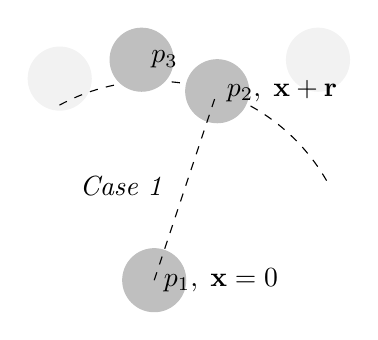
\begin{tikzpicture}[scale=0.8]
        \filldraw[ gray!10!white](+2.6,3.5)circle (0.5);
        \filldraw[ gray!10!white](-1.5,3.2)circle (0.5);
        \draw[dashed](30:3.16) arc (30:120:3.16);
        \filldraw[ gray!50!white](0,0) circle (0.5);
        \filldraw[ gray!50!white](1,3)circle (0.5);
        \filldraw[ gray!50!white](-0.2,3.5)circle (0.5);
        \draw(0,0)node[right]{$p_1, \; \textbf{x} = 0 $};
        \draw[dashed](0,0)--(1,3)node[right]{$p_2, \;\textbf{x}+\textbf{r}$};
        \draw[dashed](-0.2,3.5)node[right]{$p_3$};
        \node[ultra thick] (title) at (-0.5,1.5) {\textit{Case 1}};
    \end{tikzpicture} 
    \hfill
    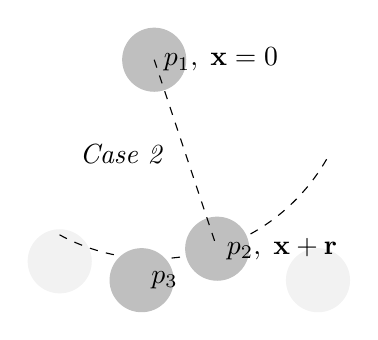
\begin{tikzpicture}[rotate=180, xscale=-0.8,yscale=0.8]
        \filldraw[ gray!10!white](+2.6,3.5)circle (0.5);
        \filldraw[ gray!10!white](-1.5,3.2)circle (0.5);
        \draw[dashed](30:3.16) arc (30:120:3.16);
        \filldraw[ gray!50!white](0,0) circle (0.5);
        \filldraw[ gray!50!white](1,3)circle (0.5);
        \filldraw[ gray!50!white](-0.2,3.5)circle (0.5);
        \draw(0,0)node[right]{$p_1, \; \textbf{x} = 0 $};
        \draw[dashed](0,0)--(1,3)node[right]{$p_2, \;\textbf{x}+\textbf{r}$};
        \draw[dashed](-0.2,3.5)node[right]{$p_3$};
        \node[ultra thick] (title) at (-0.5,1.5) {\textit{Case 2}};
    \end{tikzpicture} 
    \hfill
    % \begin{tikzpicture}[scale=0.8]
    %     \filldraw[ gray!10!white](+2.6,3.5)circle (0.5);
    %     \filldraw[ gray!10!white](-1.5,3.2)circle (0.5);
    %     \draw[dashed](-30:3.16) arc (-30:-120:3.16);
    %     \filldraw[ gray!50!white](0,0) circle (0.5);
    %     \filldraw[ gray!50!white](1,-3)circle (0.5);
    %     % \filldraw[ gray!20!white](-1.4,-3.3)circle (0.5);
    %     \filldraw[ gray!50!white](-0.2,-3.5)circle (0.5);
    %     % \draw[fill=gray,opacity=0.2](5,-0.2)circle (0.5);
    %     % \draw[fill=gray,opacity=0.2](-3,2)circle (0.5);
    %     % \draw[fill=gray,opacity=0.2](-5,0.2)circle (0.5);
    %     \draw(0,0)node[right]{$p_1, \; \textbf{x} = 0 $};
    %     \draw[dashed](0,0)--(1,-3)node[right]{$p_2, \;\textbf{x}+\textbf{r}$};
    %     \draw[dashed](-0.2,-3.5)node[right]{$p_3$};
    %     \node[ultra thick] (title) at (-0.5,-1.5) {$Case\; 2$};
    % \end{tikzpicture} 
    \caption{
        Diagram that highlights the asymmetry of the nearest pair statistics when the nearest neighbor is relatively far from the test particle.
        (\textit{Case 1}) droplet $p_1$ with  its nearest neighbor, $p_2$, located at the \underline{top} of it. 
        (\textit{Case 2}) droplet $p_1$ with  its nearest neighbor, $p_2$, located at the \underline{bottom} of it. 
        (\textit{Case 1} and \textit{2})
        In these situations, the droplet $p_2$ located at $\textbf{x} + \textbf{r}$, is the nearest neighbor of the droplet $p_1$ located at $\textbf{x}$. 
        Since $|\textbf{r}|/d$ is assumed to be large, the nearest neighbor of the droplet $p_2$ is more likely to be another nearest neighbor than $p_1$ such as the droplet $p_3$, which is closer.
        This is due to the rapid decay of $P_\text{nst}$ for large $|\textbf{r}|/d$, see \ref{fig:Pnst_high_Ga}. 
        In these cases, the nearest neighbor of $p_1$ is $p_2$, but the contrary is not true, inducing asymmetry in the statistics.  
    }
    \label{fig:diagram_asym}
\end{figure}

Now that this issue has been clarified, we can proceed to interpret the plots in \ref{fig:Why_Ga_matter}.
The beginning of the interactions happens at the early ages, meaning in the dark blue areas in  \ref{fig:Why_Ga_matter}, which are located on the top or bottom of the droplet of reference.
The ending of the interactions corresponds to the greater ages, which are represented by the red areas. 
As shown by \ref{fig:Why_Ga_matter} (left), at low \textit{Galileo} number the nearest droplet has a tendency to come from the top or bottom and leave through the sides. 
If the nearest droplet is at a reasonable distance $|\textbf{r}| < 1.5d$ on the sides of the test droplet, we can see that the vertical relative velocity is on average zero, but positive in the radial component.
In this area, the age is at its maximum (dark red zone), therefore the interactions come to an end, meaning that the nearest droplets get replaced by another. 
Note that the droplets at a larger distance of the test droplet, say $|\textbf{r}|>2$, have an averaged positive vertical relative velocity. 
As discussed above, in this situation the neighbor on the side is more likely to be closer to another droplet. 
Consequently, if the test droplet is isolated, with neighboring droplets sufficiently far on the side, it will rise on average with a lower velocity than the latter droplets.
Thus, droplets at contact seem to get apart because of the non-zero radial velocity, and droplets at a distance seem to get apart because of the non-zero vertical velocity.  
Consequently, on average the side-by-side configuration is not stable in this case, which partly explains why the droplet distribution doesn't form any layer or such oriented microstructure at these $Ga$.   

% A plausible explanation for this phenomenon is that the leading droplet accelerate the trailing droplet with its wake on a first stage. 
% Then, the trailing droplet arise to the same altitude as the leading droplet, but still goes faster than the leading droplet due to the acceleration provided by the wake of the latter droplet.
% If the droplets get in contact then the interaction duration seem to last longer, and the droplets might even get trap in a small stagnation zone on the side of the droplets.


For high \textit{Galileo} numbers, see \ref{fig:Why_Ga_matter} (right), the relative averaged velocity is nearly zero on the sides and below the test droplet. 
It is a statistical representation, meaning that, $\textbf{w}_p^r = 0$, indicates that the droplets relative  velocities are not correlated with the relative position in this area. 
Thus, it is hard to say if the area where $\textbf{w}_p^r = 0$ corresponds to actual stagnation zones where both droplets are in equilibrium, or if the relative velocity is just not correlated. 

The droplets at a large distance on the top of the test droplet have a downward velocity. 
This means that if the test sphere is isolated and approaches one or several  droplets on top of it (see \ref{fig:diagram_asym} (\textit{Case 1})), it will eventually catch up the latter droplets. 
On the contrary, if the droplet is isolated and the nearest neighbor is at the bottom (see \ref{fig:diagram_asym} (\textit{Case 2})), the velocity is either pointing downward, or it is not correlated with the position, as indicated by the magnitude of $\textbf{w}_p^r$. 
A plausible explanation for this phenomenon is that the reference droplet, when being isolated, goes faster than the potentially packed nearest neighbor.
Therefore, the test sphere can either catch up with the nearest droplet if it is above, or move further away from it if it is below.
Also, it is interesting to note that in this case the droplets at near contact on the bottom of the test droplet result from early interaction, denoted by the dark blue zone. 
It can be interpreted as follows: since 
initial duration of interaction is on average low in this zone, it does mean that droplets replace an old nearest neighbor that were at near contact with the test droplets. 
Thus, in this case, the nearest neighbor reaches the test sphere which was rising slowly because of a potentially closer neighbor. 

Ultimately, the fields $\textbf{w}^r_p(\textbf{x},\textbf{r}, a)$ provide a quantitative averaged representation of what is known as the \textit{Drafting Kissing Tumbling} \citep{fortes1987nonlinear} mechanism. 
Indeed, in both cases droplets eventually approach vertically (\textit{Drafting}), nearly touch each other (\textit{Kissing}), and leave through the sides (\textit{Tumbling}). 
Statistically, the \textit{Tumbling} part is not present in the high inertia case, which explains the creation of anisotropic structures or more stable side-by-side configurations. 
For bubble pair interactions \citet{zhang2021three} observed such DKT behavior.
They also reported side-by-side stable configurations of pairs. 
However, at the same \textit{Galileo} as \citet{zhang2021three} ($Ga = 10$) we were not able to identify this mechanism. 


To support the observations made above, we displayed in \ref{fig:unst_ga} the absolute conditioned averaged center of mass velocity of the test sphere, defined as,
\begin{equation*}
    \textbf{u}^\text{r}_p(\textbf{x},\textbf{r},t)  
    =
    \frac{1}{P_r(\textbf{x},\textbf{r},t)}
    \int_0^\infty \textbf{u}^\text{nst}_pP_\text{nst}(\textbf{x},\textbf{r},t,a) da
\end{equation*}
In \ref{fig:unst_ga} (left) we see that the magnitude of the test droplet's vertical velocity is higher than the droplet phase vertical velocity $\textbf{u}_p$ when the nearest neighbor is at near contact to the test droplet, either above or below.
\begin{figure}[h!]
    \centering
    \includegraphics[height=0.35\textwidth]{image/HOMOGENEOUS_NEW/Dist/U_l_1_Ga_10_PHI_5.pdf}
    \includegraphics[height=0.35\textwidth]{image/HOMOGENEOUS_NEW/Dist/U_l_1_Ga_100_PHI_5.pdf}
    \caption{
         Quiver plots of the conditioned droplet velocity field $\textbf{u}^\text{r}(\textbf{x},\textbf{r},t)$ colored by the averaged dimensionless vertical velocity difference : $(\textbf{u}^\text{r} - \textbf{u}_p )/ \textbf{u}_p$, for $\lambda = 1$ and $\phi = 0.05$. 
         (left) Low \textit{Galileo} number $Ga = 10$.
        (right) High \textit{Galileo} number $Ga = 100$.
         }
    \label{fig:unst_ga}
\end{figure}
When the nearest neighbor is at a large distance from the test droplet, its average velocity is lower than $\textbf{u}_p$. 
When inertia is high, however, the test droplet velocity is higher when being isolated than with its neighbor at near contact. 
Additionally, we can see that when the droplet is on the side at near contact or below, the test sphere's velocity  is lower than the mean. 
In brief in the case of $Ga = 10$ it seems that isolated droplets rise slower than close neighbors packed together. 
While at higher \textit{Galileo} number it is the opposite, we observe that isolated droplets go faster than packed neighbors. 


\subsubsection{The volume fraction dependency}
As observed in \ref{fig:A} the effect of increasing $\phi$ is that it makes the droplet distribution slightly more isotropic for $\phi >0.1$. 
\begin{figure}[h!]
    \centering
    \includegraphics[height=0.35\textwidth]{image/HOMOGENEOUS_NEW/Dist/U_rel_l_1_Ga_100_PHI_5.pdf}
    \includegraphics[height=0.35\textwidth]{image/HOMOGENEOUS_NEW/Dist/U_rel_l_1_Ga_100_PHI_20.pdf}
    % \includegraphics[height=0.35\textwidth]{image/HOMOGENEOUS_NEW/Dist/U_rel_l_10_Ga_100_PHI_10.pdf}
    % \includegraphics[height=0.35\textwidth]{image/HOMOGENEOUS_NEW/Dist/U_rel_l_1_Ga_100_PHI_10.pdf}
    \caption{Quiver plots of the relative averaged velocity field $\textbf{w}^\text{r}(\textbf{x},\textbf{r},t)$ colored by the averaged dimensionless age $a^r(\textbf{x},\textbf{r},t)$, for $Ga = 100$ and $\lambda = 1$. 
    (left) Low \textit{Galileo} number $\phi = 0.05$.
    (right) High \textit{Galileo} number $\phi = 0.2$. }
    \label{fig:Why_Phi_matter}
\end{figure}
In \ref{fig:Why_Phi_matter} we expose two situations with various volume fractions. 
In both graphs, we observe the same trend, despite the changes in length scales, which are due to the variations in volume fraction. 
Indeed, the stagnation zones with dark red color and the droplet having short ages, dark blue color, are located approximately at the same location. 
We still observe the fore-aft asymmetry with respect to the horizontal plane, as was discussed above. 
For other $\lambda$ and $Ga$ no particular differences can be observed with varying $\phi$. 
Overall, even if small differences may be present, the change in volume fraction doesn't seem to affect the relative kinematics   of interaction between droplets. 

\subsubsection{Influence of the viscosity ratio}

Lastly, we turn our attention to the effect of the viscosity ratio on pair relative kinematics. 
The question that we are trying to answer is : why does a smaller viscosity ratio increase the anisotropy of the tensor $\textbf{R}(\textbf{x},t)$ as shown in \ref{fig:A}. 
With this objective in mind, we compare two cases at $Ga = 100$ and $\phi =0.05$, where we observe a clear difference between the distributions (see \ref{fig:Pnst_high_Ga}) between $\lambda = 1$ and $\lambda = 10$.
\begin{figure}[h!]
    \centering
    \includegraphics[height=0.35\textwidth]{image/HOMOGENEOUS_NEW/Dist/U_rel_l_10_Ga_100_PHI_5.pdf}
    \includegraphics[height=0.35\textwidth]{image/HOMOGENEOUS_NEW/Dist/U_rel_l_1_Ga_100_PHI_5.pdf}
    % \includegraphics[height=0.35\textwidth]{image/HOMOGENEOUS_NEW/Dist/U_rel_l_1_Ga_100_PHI_1.pdf}
    % \includegraphics[height=0.35\textwidth]{image/HOMOGENEOUS_NEW/Dist/U_rel_l_10_Ga_100_PHI_1.pdf}
    \caption{Quiver plots of the relative averaged velocity field $\textbf{w}^\text{r}(\textbf{x},\textbf{r},t)$ colored by the averaged dimensionless age $a^r(\textbf{x},\textbf{r},t)$, for $\phi = 0.05$ and $Ga = 100$. 
    (left) High viscosity ratio $\lambda = 10$.
    (right) Low viscosity ratio, $\lambda = 1$. }
    \label{fig:Why_l_matter}
\end{figure}
As in the previous cases, it is clear that, for both cases in \ref{fig:Why_l_matter}, the neighboring droplet approaches on the vertical direction and ends its course on the sides.
As discussed previously, the case on \ref{fig:Why_l_matter} (right) exhibits a clear stagnation zone and asymmetry on a vertical plane. 
On the other hand for $\lambda =10$ the relative velocity in the vicinity of the droplet seems to be on average positive in the radial direction. 
In addition, The asymmetry aforementioned is not present in this case. 
As discussed in the previous paragraph, and explained by \ref{fig:diagram_asym}, the presence of the skew-asymmetry in the fields $\textbf{w}_p^\text{r}$ about the horizontal plane, is a sign of interactions of the isolated droplets with clusters of droplets.
The absence of such asymmetry implies the absence of such interactions, indicating that the droplets are more evenly spread. 

As before, it is interesting to investigate the value of the conditional velocity $\textbf{u}^r_p$ to better understand the droplets' collective interactions. 
Thus, \ref{fig:unst_l} display the fields  $\textbf{u}_p^\text{r}$ for both cases. 
\begin{figure}[h!]
    \centering
    \includegraphics[height=0.35\textwidth]{image/HOMOGENEOUS_NEW/Dist/U_l_10_Ga_100_PHI_5.pdf}
    \includegraphics[height=0.35\textwidth]{image/HOMOGENEOUS_NEW/Dist/U_l_1_Ga_100_PHI_5.pdf}
    \caption{
         Quiver plots of the conditioned droplet velocity field $\textbf{u}^\text{r}(\textbf{x},\textbf{r},t)$ colored by the averaged dimensionless vertical velocity difference : $(\textbf{u}^\text{r}_p - \textbf{u}_p )/ \textbf{u}_p$, for $\phi = 0.05$ and $Ga = 100$. 
         (left) High viscosity ratio $\lambda = 10$.
         (right) Low viscosity ratio, $\lambda = 1$.
         }
    \label{fig:unst_l}
\end{figure}
On \ref{fig:unst_l} (left) we first note that $\textbf{u}^\text{r}(\textbf{x},\textbf{r},t)$ behave similarly to the low inertia case displayed on \ref{fig:unst_ga} (left).
However, for $\lambda = 10$, the isolated droplets' velocity is roughly equal to $\textbf{u}_p$. 
Note that the trace of \textbf{R} is rather high in this case, (see \ref{fig:A}). 
Thus, the majority of the droplets are rather isolated. 
Consequently, if the isolated droplets rise at the average velocity of the dispersed phase it is because most of them are isolated droplets.
Therefore, this fact is not particularly relevant as it is just a statistical bias. 
Nevertheless, we can still conclude that for $\lambda = 10$ droplets go faster with a nearest neighbor on top or bottom, while for  $\lambda = 1$ droplets go faster when the nearest neighbor is at a large distance. 

\subsubsection{Relation with the dispersed phase velocity fluctuation tensor}

In addition to providing physical explanations, the field $\textbf{u}_p^d = \textbf{u}^r_p - \textbf{u}_p$ is of great importance to study the droplet phase fluctuation tensor $\pavg{\textbf{u}_i' \textbf{u}_i'}$ which is of crucial importance in multiphase flow modeling. 
Indeed, it can be shown that 
\begin{equation}
    \frac{\pavg{ \textbf{u}_i' \textbf{u}_i'}}{n_p}(\textbf{x},t)
    =  
    \int_{\mathbb{R}^3 }
    \textbf{u}_p^d
    \textbf{u}_p^d
    P_{nst}(\textbf{r}|\textbf{x},t)
    d\textbf{r}
    + \int_{\mathbb{R}^3 }
    \textbf{F}(\textbf{r},\textbf{x},t)
    d\textbf{r}
    \label{eq:particle_center_of_mass_velocities}
\end{equation}
where, $\textbf{F} = \avg{\sum_i\sum_{j\neq i}\delta_j\delta_i h_{ij}(\textbf{u}_i - \textbf{u}_p^{nst})(\textbf{u}_i - \textbf{u}_p^{nst})}$. 
Thus, the ensemble-averaged dispersed phase Reynolds stress is the sum of the fluctuation given by $\textbf{u}_p^r$ plus an additional contribution from the other droplet velocity fluctuations around the average field $\textbf{u}_p^d$. 
At low volume fraction, it is reasonable to think that the former term represents the majority of the droplet phase fluctuation.\footnote{
    However, note that it is note true in Stokes regime as the contribution from the second, third \ldots nearest droplets will become non-negligible even in the dilute regime. 
} 
Therefore, \ref{fig:unst_l} constitutes a visual representation of the droplet phase agitation tensor $\avg{\delta_i \textbf{u}_i' \textbf{u}_i'}$. 
Notably, we can remark on \ref{fig:unst_l}  that the droplet phase fluctuations tensor seems to be anisotropic. 
Indeed, more vertical velocity fluctuations than horizontal one is observed. 
This implies that the ``granular temperature'' $k_p = \pavg{ \textbf{u}_i' \cdot \textbf{u}_i'}/(2n_p)$ is probably not sufficient to model $\avg{\delta_i \textbf{u}_i' \textbf{u}_i'}$ in buoyant emulsions. 

Based on \ref{eq:particle_center_of_mass_velocities} we can compute the variance of the velocity of sedimenting suspensions of spherical droplets in Stokes and dilute regimes.
The method is quite similar than what is done in \citet{zhang2021ensemble} and \ref{chap:pseudoturbulence}. 
This idea will be pursued in a future study. 


\subsubsection{Discussion}
% \tb{
%     The field $\textbf{w}_p^r$ is useful for several reasons. 
%     As discussed it might serve to close equations such as \ref{eq:dt_R}. 
%     Or simply it provides us with clear physical explanation of what particles interaction look like. 
%     Also, we believe that it might be useful for coalesce kernels modeling. 

    
% }

From \ref{sec:Theory} we demonstrated that $\textbf{R}(\textbf{x},t)$ follows a transport equation where the tensor $\textbf{W}(\textbf{x},t)$ acts as a source term. 
This tensor might be expressed as the symmetric part of $\int_0^\infty \textbf{r} \textbf{w}_p^\text{r} P(\textbf{x},\textbf{r},t) da$. 
Thus, the trends of the $\textbf{w}_p^\text{r}(\textbf{x},\textbf{r},t) $ in terms of the position determine the value of $\textbf{W}(\textbf{x},t)$ and partly determine the final value of $\textbf{R}(\textbf{x},t)$. 
In many of the graphs, we observed that the vertical components of $\textbf{w}_p^\text{r}$ were negative when the vertical component of \textbf{r} was positive and vice versa. 
Consequently, $W_{yy}$ must be on average negative and $W_{xx}$ positive,this et  which ultimately contributes to the value of $\textbf{R}(\textbf{x},t)$ and $\textbf{A}(\textbf{x},t)$ through \ref{eq:dt_R} and justifies the sign of $A_{xx}$ in \ref{fig:A}. 

In \ref{fig:phase} we display the values of $W_{xx}$ in terms of $Ga$ and $\phi$. 
These graphs provide us with a concise description of the relative kinematics. 
We recall that $\textbf{W}:\bm\delta = 0$ as we demonstrated in \ref{sec:Theory}, thus the value  $W_{xx}$ entirely determines $W_{yy}$ since the problem is symmetric. 
For example, we see that the highest dimensionless relative velocity position is reached for $Ga = 10$ and $\phi = 0.01$. 
This implies that, it is in the dilute regime and with relatively small inertial effects, that the particles have the fastest relative motions. 
\begin{figure}[h!]
    \centering
    % \begin{tikzpicture}[scale=0.8]
    %     \node (img) at (0,0) {\includegraphics[height=5.5cm]{image/HOMOGENEOUS_NEW/PA/phase_Wxx_l_1.pdf}};
    %     \node (img) at (11,0) {\includegraphics[height=5.5cm]{image/HOMOGENEOUS_NEW/PA/phase_Wxx_l_10.pdf}};
    % \end{tikzpicture}
    \includegraphics[height=5.5cm]{image/HOMOGENEOUS_NEW/PA/phase_Wxx_l_1.pdf}
    \includegraphics[height=5.5cm]{image/HOMOGENEOUS_NEW/PA/phase_Wxx_l_10.pdf}
    \caption{Phase diagram of the horizontal components of the dimensionless correlation tensor $W_{xx}/(Ud)$. 
        (left) Iso-viscous emulsion $\lambda = 1$.
        (right) Viscous droplets $\lambda = 10$ }
    \label{fig:phase}
\end{figure}
Is the relative velocity fields $\textbf{w}_p^r$ the cause of the microstructure shape as is suggested by \ref{eq:dt_R}. 
Or does $\textbf{w}_p^r$ the consequence of microstructure shape? 
As suggested by the previous graphs \eqref{fig:Why_Ga_matter,fig:Why_l_matter,fig:Why_Phi_matter}. 
Indeed, on \ref{fig:Why_l_matter} (right), the clear asymmetry with respect to the horizontal plane can be explained as the consequence of clusters in the flows. 
Although it is a complicated question, we believe that both are true, even if physical parameters also impact $\textbf{w}_p^r$, which makes the microstructure case dependent.  
Nevertheless, this makes $\textbf{W}(\textbf{x},t)$ potentially a function of $\textbf{R}(\textbf{x},t)$.
Depending on its relationship with $\textbf{R}(\textbf{x},t)$ this may modify the relaxation time.  
Thus, a more efficient way to close \textbf{W} in an objective manner would be to study the dynamic of interactions. 
In this work, we only provided kinematics   arguments to explain the microstructure shape. 
Of course to fully understand the physics of interaction one has to study the dynamics of interactions. 
It is in fact possible in our framework to include such dynamics variable by deriving an equation for \textbf{W} the same way we derived \ref{eq:dt_R} for \textbf{R}.
Thus work is still needed to fully understand interaction dynamics within this ``nearest-particle statistics'' framework. 




% \subsection{Carrier phase velocity fields}

In the previous section we explained the microstructure formation with kinematic arguments.
Although we indeed provided an explanation the question that arise now id :
Why does the relative velocity behave as such.
The answer might be obtained based on dynamical arguments as it is done often, in such a way we could explain the relative kinematic.
Nevertheless, the dynamical aspect of the interaction is out of the scope of this study and will be treated in a future work. 

Instead, we propose to study the particles averaged wakes to explain the possible difference in interaction between the iso-viscous and viscous droplets cases. 
Again we make use of the nearest particle averaged statistic to compute the carrier fluid phase velocity conditionally on the presence of a particle at \textbf{x}, it reads,
\begin{equation*}
    \textbf{u}^\text{nst}_f P_{nst}(\textbf{x},\textbf{r},t)= 
    \int \sum_{i}^{N_b} \delta(\textbf{x}-\textbf{x}_i(\FF,t))
    h_{i} 
    \textbf{u}_f^0(\textbf{x}+\textbf{r},t,\FF)
    d\mathscr{P} 
\end{equation*}
where $h_{i} = 1$ if the particle $i$ center of mass is the nearest point to the eularian coordinate \textbf{x}+\textbf{r}. 
This velocity fields can be reconstructed as well with our DNS. 
On \ref{fig:stream} we display the reconstructed velocity field $\textbf{u}^\text{nst}_f$ for (left) the iso-viscous case $\lambda =1$ and (right) the viscous droplets' case $\lambda = 10$, for different value of the volume fraction. 
\begin{figure}[h!]
    \centering
    \includegraphics[height=0.4\textwidth]{image/HOMOGENEOUS_NEW/Stream/Stream_PHI_1_Ga_100_l_100}
    \includegraphics[height=0.4\textwidth]{image/HOMOGENEOUS_NEW/Stream/Stream_PHI_1_Ga_100_l_10}
    \includegraphics[height=0.4\textwidth]{image/HOMOGENEOUS_NEW/Stream/Stream_PHI_5_Ga_5_l_100}
    \includegraphics[height=0.4\textwidth]{image/HOMOGENEOUS_NEW/Stream/Stream_PHI_5_Ga_5_l_10}
    \includegraphics[height=0.4\textwidth]{image/HOMOGENEOUS_NEW/Stream/Stream_PHI_20_Ga_100_l_100}
    \includegraphics[height=0.4\textwidth]{image/HOMOGENEOUS_NEW/Stream/Stream_PHI_20_Ga_100_l_10}
    % \includegraphics{image/HOMOGENEOUS_NEW/Stream/Stream_PHI_5_Ga_100_l_1.pdf}
    \caption{Nearest averaged carrier phase velocity fields. }
    \label{fig:stream}
\end{figure}
This velocity field is evaluated at $\textbf{x}+\textbf{r}$ conditioned on the presence of the nearest particle at $\textbf{x}$. 


\tb{compare with \citet{shajahan2023inertial} for explaination }

\section{Conclusion}
\section{Conclusion}

% \citet{einstein1905neue,taylor1932viscosity} demonstrated how the first moment of the hydrodynamic forces (Stresslet) applied on a particle immersed in pure linear flow induced an additional viscosity to the mixture. 
% Later~\citet{zhang1994ensemble,lhuillier1996contribution,jackson1997locally,zhang1997momentum} demonstrated that the second moment of forces were also contributing to the stresses inducing a non-newtonian behaviors, even in the Stokes and dilute limit.  

In this work we computed the moments of force on the surface of a test droplet in the situation of uniform relative motions between the droplet and the continuous phase. 
We considered low but finite Reynolds number $Re$. 
The averaged first moment of force is given by~\ref{eq:forces_reformulated2_avg}, scales as $O(\rho_f \phi u_r^2)$, hence contributing to the averaged Stress of the suspension on the same ground as  \citet{einstein1905neue} or \citep{taylor1932viscosity} correction to the viscosity of the mixture. 
In a lesser extend the inertial part of the second moment also contribute to the Rheology. 
This first point constitutes the main result of the paper. 

Others important conclusion reached through this work includes: a general reciprocal formula to derive the forces and moments on droplets, and the explicit appearing of the velocity variance term in the drag force term. 








\chapter{Closure modeling}
\label{chap:mono-disperse}
\localtableofcontents


\section{Average drag force}

%Objectives : 
%\begin{itemize}
%    \item Present the rising velocity Vs. phi to demonstrate the relation with $\phi^{1/3}$ \citep{loisy2017buoyancy}
%    \item Discus the common points and differences with bubbles and solid particles. 
%    \item Present a proper definition of the drag force terms such as in \citet{wang2021numerical}. 
%    \item Discus the possible correlation between the shape /arrangement of the particles/flow lines with the rising velocity. \tb{Je ne sais pas trop quoi dire la dessus}
%    \item Show that \citet{rusche2000effect}'s fit for the drag force is not adapted for our case and propose a new one
%    \item All the references for teh Drag force terms are in \citet[chap 8]{morel2015mathematical} or in \citet{ishii2010thermo}
%\end{itemize}
%\todo[inline]{include fits of bubbly flow}

\subsection{Terminal velocity of an isolated spherical drop}
%First of all we want to investigate the dependency of the drift velocity with the volume fraction $\phi$. 
%It is known from several studies on the litterature, especially in \citep[chapter 8]{morel2015mathematical} and \citet[chapter 12]{ishii2010thermo} the the viscosity model for various system can be written generally, as,
%\begin{equation*}
%    \frac{\mu_m}{\mu_c}
%    = \left(
%        1 - \frac{\phi}{\phi_\text{max}}
%    \right)^{-2.5 \phi_\text{max}\mu_\text{eq}}
%\end{equation*}  
%with, $\mu_\text{eq} = \frac{\mu_d + 0.4 \mu_c}{\mu_d+\mu_c}$ and $\phi_\text{max}$ being the volume fraction corresponding to the \textit{maximum packing}. 
%\JL{la viscosite d'une suspension n'a rien a voir avec sa vitesse de chute meme si cela semble etre un argument donne dans la litterature... j'ai enleve tout cela pr l'instant}

In this part, we briefly review the various formulas used to calculate the drag force on a spherical droplet embedded in a steady uniform flow. As demonstrated in Appendix \ref{app:shape} the droplet remains approximatively spherical. This assumption remains valid for the whole range of parameters investigated even in high inertial regime where the maximum deviation from the spherical shape is around $10$ \%. Theoretical predictions for the force on a spherical droplet embedded in a steady uniform flow are limited to the limit of very small and very high Reynolds numbers. We define the drag coefficient, denoted as $C_D$ by the equation $F = \pi / 8 C_D \rho U_0^2 d^2$, where $F$ is the force on the drop, $U_0$ is the imposed velocity. The drag coefficient is a function of the Reynolds number $Re = \rho U_0 d /\mu $ and of is the viscosity ratio$\lambda = \mu _d /\mu _c$. % is the  as $F = C_D$ 
In the Stokes regime ($Re=0$)the drag coeficient is given by the Hadamard-Ribczynski formula


%In this section, we briefly survey the diverse formulas applied to calculate the drag force acting on a spherical droplet within a steady, uniform flow. As corroborated in Appendix \ref{app:shape}, the droplet maintains an approximate spherical shape, a validity sustained across the entire spectrum of investigated parameters, even in the high inertial regime. Theoretical predictions for the force acting on a spherical droplet in a steady uniform flow are confined to scenarios of extremely low and exceptionally high Reynolds numbers.

%We define the drag coefficient, denoted as $C_D$, by the equation F=π8CDρU02d2F = \frac{\pi}{8} C_D \rho U_0^2 d^2F=8π​CD​ρU02​d2, where FFF signifies the force on the droplet, and U0U_0U0​ is the imposed velocity. This coefficient varies with the Reynolds number Re=ρU0dμRe = \frac{\rho U_0 d}{\mu}Re=μρU0​d​ and the viscosity ratio λ=μdμc\lambda = \frac{\mu_d}{\mu_c}λ=μc​μd​​. In the Stokes regime, the drag coefficient adheres to the Hadamard-Ribczynski formula.

%In the Stokes flow regime, the drag coefficient defined as $F = $

%drag force on a spherical drop embedded in a steady uniform flow is given by the Hadamard-Ribczynski formula
%\JL{il faut choisir ton echelle caractersitique de longueur. Soit $a$ le rayon soit le diametre des particules.}
%\begin{equation}
%F_0 = -\pi \mu d U \frac{2+3\lambda}{1+\lambda}
%\end{equation}

\begin{equation}
C_D = \frac{8}{Re} \left( \frac{2+3\lambda}{1+\lambda} \right)
\end{equation}
%\ref{fig:U} shows the drift velocity $U$ divided by the stokes rising velocity of a spherical droplet $U_\text{stokes}$ defined in our notation as \citep{kim2013microhydrodynamics}, 
Balancing the drag force obtained using the previous formula with the buoyancy force one obtained the settling velocity in the Stokes regime
\begin{equation}
    U_0
    = (\rho_c - \rho_d)\frac{g d^2}{6\mu_c}\left(\frac{1+\lambda}{2 + 3\lambda}\right),
\end{equation}
or in dimensionless form 
\begin{equation}
    Re_0
    = \frac{Ar^2}{6}\left(\frac{1+\lambda}{2 + 3\lambda}\right).
\end{equation}
where $Re_0 = \rho_c U_0 d/\mu_c$ is the Reynolds number based on the terminal velocity.
In the opposite regime of very high Reynolds numbers ($Re\gg 1$), the flow outside the droplet can be considered as potential except in a thin boundary layer developing on the bubble surface. \citet{harper1968} have shown that the drag coefficient on a spherical drop is given by 

\begin{equation}
C_D = \frac{48}{Re}\left(1 + \frac{3\lambda}{2}\right).
\label{eq:harper}
\end{equation}
Equation \ref{eq:harper} is the leading order in the expansion performed by \citet{harper1968} in the limit $Re\gg 1$. This equation tends toward Levich formula for the drag on a clean bubble in the limit $\lambda \ll 1$. A detailed investigation perfomed by Dandy et Leal have shown that the oroginal formulation by Harper and mmore became accurate for $Re\geq 200$. The above review show that in the intermediate Reynolds number regimes of the pressent study $ 1 \leq ...$

\begin{equation}
C_D = \frac{24}{Re}(1+0.15Re^{0.687})
\end{equation}

\begin{equation}
C_D = \frac{16}{Re}\left(1+\left[\frac{8}{Re}+\frac{1}{2}\left(1+3.315Re^{-1/2}\right)\right]^{-1}\right)
\end{equation}


\begin{equation}
C_D(Re)Re^2=\frac{4}{3}Ga ^2
\label{}
\end{equation}


%where higher order terms can be found in the original publication of \citet{harper1968}. 

%to leading order as $Re = \rho U_0 d /\mu$ 


In practice the above formula are very limited randge of validity and empirical formulation have to be used for intermediate Reynolds numbers. Prendre la correlation de Rykind et Ryskin



\subsection{Hindered settling velocity}
As an exemple for a suspenison of homogeneous solid spherical particle $\phi_\text{max} = 0.62$ and for deformable particles system it can be approximated to $\phi_\text{max} = 1$. 
From this consideration we can deduce that the drift velocity $U$ is related to the volume fraction with, 
\begin{equation*}
    \frac{U(\phi)}{U_\text{stokes}} = \left\{\begin{tabular}{cc}
        $(1-\phi)^{1.5}$   & bubbles in liquid \\
        $(1-\phi)^{2.25}$   & drops in liquid \\
        $(1-\phi)^{3}$   & drops in gas \\
    \end{tabular}\right.
\end{equation*} 
Additionally, \citet{bunner2003effect} propose a scaling of $\sim (1 - \phi^{1/3})$ for spherical bubbles.
While \citet{ishii1979drag} proposed a $\sim (1 - \phi)^3$ for deformable bubbles. 

In our case, i.e. quasi spherical droplets, we reach a $\sim (1 - \phi^{1/3})$ scaling for $\lambda = 10$ and approximately a $\sim (1 - \phi^{1/2})$ scalings for $\lambda = 1$ .
\begin{figure}[h!]
    \centering
    \includegraphics[height = 0.35\textwidth]{image/HOMOGENEOUS/fCA/UstokesGa_mu_r_1-0.pdf}
    \includegraphics[height = 0.35\textwidth]{image/HOMOGENEOUS/fCA/UstokesGa_mu_r_0-1.pdf}
    \caption{Rising velocity divided by the rising velocity of an equivalent spherical drop in Stokes regime.($\bullet$) $Ga = 5$, ($\blacktriangle$) $Ga = 10$, ($\blacksquare$) $Ga = 25$ , ($\blacklozenge$) $Ga = 50$, ($\blacktriangleright$) $Ga = 75$ and ($\blacktriangleleft$) $Ga = 100$ . 
    The dashed lines are the empirical funtions (left)  
    $U/U_\text{stokes} = 2.72(Ga^{-2.77} - Ga\;10^{-3}) (1 - \phi^{0.45})$
    (right)  $U/U_\text{stokes} = 2.74(Ga^{-2.85} - Ga \;10^{-3}) (1 - \phi^{0.34})$ }
    \label{fig:U}
\end{figure}

The case for which $\lambda = 1$ have a tendency to processes more deformation, as caracterised by their averaged aspect ratio $\chi$ slightly higher than those for which $\lambda = 10$. 
The differences in the volume fraction dependency can be partially explain by this fact. 
Indeed, a  $\sim (1 - \phi^{2/3})$ power law were observed for slightly deformable bubbly flow \cite{zhang2021direct}. 
Thus it is not surprising that at low but finite deformation we found a scalings between $1/3$ and $2/3$. 

A last interesting fact is that at low $Ga$ and $\phi$ we observe a rising velocity $U / U_\text{stokes} > 1$ meaning that the rising velocity is higher than in the stokes isolated case. 
This phenomena has already been observe in \citet{loisy2017buoyancy}. 
This fact was explained to be due to the cumulative effect of the wakes in orderred array of bubbles  which tends to increases their colective velocity. 
Anyhow, since the the limit $Ga \rightarrow 0$ and $\phi \rightarrow 0$ we must recover $U/U_\text{stokes} = 1$ we can be sure that the $\phi$ scaling won't behaves like so.
Therefore it is crucial to point out that these scalings are surely not valid in the limit  $Ga \rightarrow 0$ and $\phi \rightarrow 0$ .

%\subsection{Interphase drag force}




Now we present our results for the drag force term in terms of the Reynolds number. 
\begin{figure}[h!]
    \centering
    
    \includegraphics[height = 0.35\textwidth]{image/HOMOGENEOUS/fCA/Re_mu_r_1-0.pdf}
    \includegraphics[height = 0.35\textwidth]{image/HOMOGENEOUS/fCA/Re_mu_r_0-1.pdf}
    
    \includegraphics[height = 0.35\textwidth]{image/HOMOGENEOUS/fCA/Fstokes_N_5_l_1.pdf}
    \includegraphics[height = 0.35\textwidth]{image/HOMOGENEOUS/fCA/Fstokes_N_5_l_10.pdf}
    \caption{
        (middle) Reynolds number based on the averaged rising velocity.
    (bottom) Ensemble averaged drag force divided by the stokes drag force on spherical droplet of equivalent size.
    The symbols correspond to different volume fraction ($\bullet$) $\phi = 1\%$, ($\blacktriangle$) $\phi = 5\%$, ($\blacksquare$) $\phi = 10\%$, ($\blacklozenge$) $\phi = 15\%$ and ($\blacktriangleright$) $\phi = 20\%$.
    (dashed lines) empirical formulas : extrapolation of  \citet{tenneti2011drag} for solid particles. }
    \label{fig:drag_force}
\end{figure}
\tb{As discussed in previous study that
for spherical bubbles, as the gas fraction increases and the in-
teractions become more important, the bubbles tend to align
themselves in horizontal pairs, whose average rising velocity
is lower than that of an isolated bubbl}

The interphase drag forces applied on the droplets is the buoyancy force $(\rho_d-\rho_c)v_\alpha \textbf{g}$.
The relevant quantity is therefore the dimensionless drag force, that is what is presented in the following \ref{fig:drag_force}. 


In the stokes regime the drag force on a spherical droplet is, 
\begin{equation*}
    \textbf{F}_s
    =\pi \mu_f d (\textbf{u}_p - \textbf{u}_c) \left(\frac{2+3\lambda}{1+\lambda}\right)
\end{equation*}
Let the dimensionless drag force be a function of $\lambda$ $Re$ and $\phi$, expressed such that, 
\begin{equation}
    \textbf{f}_p(Re,\phi,\lambda)
    = 
    f_1^*(Re)
    f_2^*(\phi)
    \textbf{f}_s(\lambda)
\end{equation}
where $f_{1,2}$ are coefficient which limit tends to $1$ at low $\phi$ and low $Re$. 
To determine the $\phi$ dependency we base our study on the following analysis. 
In \cite[chapter 4]{ashgriz2011handbook} they stipulate that the last droplets empirical fit was made in the study of \citet{rusche2000effect} where they performed empirical fits on experimental datas of emulsion. 
Some of which concerned droplets' sedimentation, were they stipulate that, 
\begin{align*}
    f_1^*(\phi) 
    &=1  + C_1 Re^{C_2}\\
    f_2^*(\phi) 
    &= e^{\phi K_1} + \phi K_2
    \label{eq:drag_fit}
\end{align*}
Nevertheless, the coefficients for the droplets doesn't agree with our numerical calculation. 
Instead we remark that the solid particles fit from \citet{rusche2000effect} well fits our results at $\lambda = 1$. 
Therefore, we propose to keep the shape of teh fits and adjuste our coefficient. 

\tb{Dans cette partie je ne sais pas trop quoi faire pour avoir un bon point de départ pour cree une formule empirique, je manque d'idée, notament pour ce qui est de la dépendence en $\lambda$ et pour l'explication physique des tendence observe. }

%\subsection{Interphase drag force}
%\subsection{Droplets configurations flowlines and deformations }

\section{The Reynolds stress}

Objectives : 
\begin{itemize}
    \item Present the decomposition of the fluid reynolds stress according to isotropic and deviatoric part.
    \item Show the relation between the flowlines graphs and the actual values of the fluid velocity fluctuation.
    \item Compare our case with the fits of  \citet{almeras2019fluctuations} 
    \item Compare the fluctuation with theoretical dev \citet{lance1991turbulence,zhang1994ensemble}. 
    \item Find out that the potential flow solution 
    \item Conclusion : " In low inertia regime $B_{xx} = - 0.2$ and $B_{yy} = 0.4$ for all simulations, find out why" (This is also true for the theoretical solution\citep{lance1991turbulence} this is thus due to the form of teh wake)
\end{itemize}


In this section we analyze the velocity fluctuation within the suspension for both phases. 
We decompose both Reynolds stresses into an isotropic part and deviatoric part such that, 
\begin{align}
    \bm{\sigma}^{\text{Re}}_p &=  \rho_d \phi_d K^*_p(\textbf{u}_p - \textbf{u}_c)\cdot (\textbf{u}_p - \textbf{u}_c) 
    \left(
        \textbf{I}
        +\textbf{B}_p 
    \right)\\
    \bm{\sigma}^{\text{Re}}_c &=  \rho_c \phi_d K_c^*(\textbf{u}_p - \textbf{u}_c)\cdot (\textbf{u}_p - \textbf{u}_c) 
    \left(
        \textbf{I}
        +\textbf{B}_c
    \right)
\end{align}
where the $K^*$ is the dimensionless pseudo-turbulent  kinetic energy, $\textbf{I}$ a unit tensor and $\textbf{B}$ a tensor accounting for the deviation of the Reynolds stress left to determine. 
In the following subsection we present our numerical results for $K^*$ and $\textbf{B}$ for the dispersed and continuous phase. 
\tb{In this section the results are presenetd in terms of Ga because it is easier to show the tendency}

Alternatively we can use the decomposition,
\begin{align}
    \phi_c\bm{\sigma}^{\text{Re}}_c &=  \rho_c \phi_d 
    \left[
        B_1\textbf{I}(\textbf{u}_p - \textbf{u}_c)\cdot (\textbf{u}_p - \textbf{u}_c) 
        +B_2 (\textbf{u}_p - \textbf{u}_c) (\textbf{u}_p - \textbf{u}_c) 
    \right]\\
\end{align}
for which $B_1$ and $B_2$ are scalar coefficient. 
This decomposition has the advantage that in the potential flow limit theoretical solution are known such that  $B_1 = -0.15$ and  $B_2 = 0.05$ \citet{zhang1994averaged,wang2021numerical}. 
Lastly, \citet{lance1991turbulence} give also a theoretical solution for $\bm{\sigma}^{Re}_c$ based on the potential flow solution around a spherical particle in translation. 


\subsection{Continuous phase}
\todo{try \citet{almeras2021statistics} fits}
\todo{also check \citet{almeras2019fluctuations} results}
\tb{might be good to plot the velocity field to examine where does the fluctuation arise (pseudo-turbe or turbe)}
Look at \citep{wang2021numerical} and Mahra.. 2015 



The fluid averaged kinetic energy can be easily scaled on the numerical results shown \ref{fig:Tf_Bf}(left).
It is shown that for $\lambda= 1$ we observe non monotonic behavior while at $\lambda= 10$ it is decreasing.
Except for the cases $\phi = 0.01$ where we cannot be sure if it is due to statistical error or real physics. 
\begin{figure}[h!]
    \centering
    \includegraphics[height=0.3\textwidth]{image/HOMOGENEOUS/fCA/Tf_l_1.pdf}
    \includegraphics[height=0.3\textwidth]{image/HOMOGENEOUS/fCA/Bf_l_1.pdf}

    \includegraphics[height=0.3\textwidth]{image/HOMOGENEOUS/fCA/Tf_l_10.pdf}
    \includegraphics[height=0.3\textwidth]{image/HOMOGENEOUS/fCA/Bf_l_10.pdf}
    \caption{(left) Dimensionless turbulent kinetic energy in terms of the \textit{Galileo} number for different $\phi$. (dots) Numerical simulations, (dashed line) empirical formula \ref{eq:Tf_scaling}.
    The symbols correspond to different volume fraction ($\bullet$) $\phi = 1\%$, ($\blacktriangle$) $\phi = 5\%$, ($\blacksquare$) $\phi = 10\%$, ($\blacklozenge$) $\phi = 15\%$ and ($\blacktriangleright$) $\phi = 20\%$.
    (right) deviatoric part of the Reynolds stress, ($- \cdot -$)  vertical components, $B_{yy}$, ($- -$)  horizontal components, $B_{xx} = B_{zz}$.}
    \label{fig:Tf_Bf}
\end{figure}
\subsection{Dispersed phase}

\tb{Maybe include velocity fluctuation and compare to : Lingxin2021 }

\tb{Include Gaussian distribution of bubbles !!! ! ! ! }

Now let's focus on the particular averaged Reynolds stress tensor.
\ref{fig:Talpha_Balpha} shows that the granular temperature behavior is quite similar from the continuous averaged turbulent kinetic energy.
\begin{figure}[h!]
    \centering
    \includegraphics[height=0.3\textwidth]{image/HOMOGENEOUS/fPA/Talpha_l_1.pdf}
    \includegraphics[height=0.3\textwidth]{image/HOMOGENEOUS/fPA/Balpha_l_1.pdf}

    \includegraphics[height=0.3\textwidth]{image/HOMOGENEOUS/fPA/Talpha_l_10.pdf}
    \includegraphics[height=0.3\textwidth]{image/HOMOGENEOUS/fPA/Balpha_l_10.pdf}
    \caption{(left) Dimensionless turbulent kinetic energy $K_p$ in terms of the \textit{Galileo} number for different $\phi$. 
    The symbols correspond to different volume fraction ($\bullet$) $\phi = 1\%$, ($\blacktriangle$) $\phi = 5\%$, ($\blacksquare$) $\phi = 10\%$, ($\blacklozenge$) $\phi = 15\%$ and ($\blacktriangleright$) $\phi = 20\%$.
    (right) deviatoric part of the Reynolds stress, ($- \cdot -$)  vertical components, $B_{yy}$, ($- -$)  horizontal components, $B_{xx} = B_{zz}$.}
    \label{fig:Talpha_Balpha}
\end{figure}


% \chapter{Mono-disperse buoyant water/oil emulsion.}
\label{chap:mono-disperse}

In this chapter we present the results related to the mono-disperse buoyant rising  emulsion of droplets.
All the simulations files can be found here \url{http://basilisk.fr/sandbox/fintzin/Rising-Suspenion/}
This chapter will cover the different closure terms that we brought to light in \ref{chap:avg}, such as the mean slip velocities or drag force, the Reynolds stress tensor and the particle stress tensor.
Even through we forced non coalesce in these simulations we will still discuss the possibility to close the collision kernel of PBE or Lagrangian equations. 
Also in this chapter we will solely focus on the momentum equations closure, and neglect mass transfer terms. 
\begin{figure*}
    \centering
    \includegraphics[width = 0.8 \textwidth]{image/PHI_01_Ga_75.png}
    \caption{Snapshot of a simulation at $T_g = 300$ for $\phi = 0.1$, $Ga = 75$ $\mu_r = 0.1$ and $N_b = 125$. In white : the interfaces, The background color map correspond to the pressure field. The grid represents the different core.}
    \label{fig:pic_sim}
\end{figure*}
As a consequence of the mono-disperse assumption it is evident that the mass balance and number density balance are similar. 
However, the surface balance (\ref{eq:A_avg_p}) remains relevant as the surface of all particles is not constant since it is a function of the deformation. 
However, as it will be shown in the low \textit{Bond} numbers limit the droplets remain spherical allowing us o discard this equation too. 
Therefore, In this context we be interested in the momentum balance's (\ref{eq:classic_hybrid_momentum_p} and \ref{eq:classic_hybrid_momentum_c}) closures. 
Neglecting the mass transfer terms and considering the mass as a constant yields the following particular and continuous averaged momentum equations, 
\begin{multline}
    \rho_c\pddt (\phi_c\cavg{\textbf{u}}) 
    + \rho_c\nablab \cdot ( \phi_c \cavg{\textbf{u}}\cavg{\textbf{u}})
    = \pavg{\int_{S_\alpha} \textbf{T}_c  \cdot \textbf{n}_c d S}
    +\phi_c\cavg{\textbf{b}}\\
    + \nablab\cdot\left[
    \phi_c \cavg{\textbf{T}}
    - \pavg{\int_{S_\alpha} \textbf{r} \textbf{T}_c  \cdot \textbf{n}_c dS}
    - \rho \cavg{\textbf{u}'\textbf{u}'}
    \right],
    \label{eq:homo_momentum_c}
\end{multline}
\begin{multline}
    \pddt   \left(\pavg{\textbf{u}_\alpha}\right)
    + \nablab \cdot \left(\pavg{\textbf{u}_\alpha}\pnavg{\textbf{u}_\alpha}\right)
    = \frac{n}{m_\alpha}\pnavg{\int_{V_\alpha} \textbf{b} dV}\\
    + \frac{n}{m_\alpha}\pnavg{\int_{S_\alpha} \textbf{T}_c  \cdot \textbf{n}_c dS}
    - \nablab \cdot \left(\pavg{\textbf{u}_\alpha' \textbf{u}_\alpha'}\right). 
    \label{eq:homo_momentum_p}
\end{multline}
From these simplified equations we can start to complete the closure problem.

Since all simulations reach as quasi static regime we can stipulate that the averaged velocities vector are constants and vertical. 
Therefore, all along this chapter we note the drift velocity such as $U = \pnavg{\textbf{u}} - \cavg{\textbf{u}}$. 
Besides, in this chapter we fix the following dimensionless parameters to $\rho_r =1.11 $, $\mu_r =0.1$, $Bo =1$ and $N_b = 125$. 
As a consequence of the small \textit{Bond} number in presence, the droplets are nearly spherical. 
A picture of a typical simulation is shown \ref{fig:pic_sim}
% \section{The drag force term}
We start by the drag force term. 
Our simulations reach a quasi steady regime meaning that we can consider the velocities of the particular phase and fluid phase as constant.
Now lat's place our selves in the reference frame moving at the averaged velocity of the particles. 
In this frame of reference the particles are thus fixed and see the fluid flowing through, experiencing a drag force due to the stress on the droplets surface. 
Therefore, in this referential considering $\pavg{\textbf{u}} = \textbf{0}$, the momentum equation \ref{eq:homo_momentum_p} yields, 
\begin{equation*}
    m_\alpha \nablab \cdot \left(\pavg{\textbf{u}_\alpha' \textbf{u}_\alpha'}\right). 
    = \pavg{\int_{V_\alpha} \textbf{b} dS}
    + \pavg{\int_{S_\alpha} \textbf{T}_c  \cdot \textbf{n}_c dS}
\end{equation*}
\tb{to be disscused}
We can observe that the divergence of the fluctuation is balanced by the two contributions to the RHS.  
Besides, the body force term has the simple expression, $\pavg{\int_{V_\alpha} \textbf{b} dV} = - nV_\alpha (\rho_d-\rho_c) \textbf{g}$. 
Therefore, the drag force term must be expressed as the sum of a pure drag force which balance the body force and a divergence of a stress which balance in this can the Reynolds stress \citep{zhang2021ensemble,wang2021numerical,nott2011suspension}. 
In this section we focus on the pure drag component and expresses it in the dimensionless form such as, 
\begin{align*}
    \pnavg{F_\mu}
    = \frac
    {\pnavg{\int_{V_\alpha} \textbf{T}\cdot \textbf{n}dV}}
    {\mu_c U D}
    = \frac
    {\left(\rho_d -\rho_c\right) \textbf{g}}
    {\mu_c U}D^2
\end{align*}
Where $\pnavg{F_\mu}$ is the pure dimensionless drag force along the direction of the velocity. 

\ref{fig:f_mu} displays the interphase drag force for different \textit{Galileo} number and volume fraction. 
\begin{figure}[h!]
    \centering
    \includegraphics[height=0.3\textwidth]{image/HOMOGENEOUS/fCA/FH_mu_Ga.pdf}
    \includegraphics[height=0.3\textwidth]{image/HOMOGENEOUS/fCA/UstokesGa.pdf}
    \caption{(left) Dimensionless drag forces in terms of the \textit{Galileo} number for different volume fraction $\phi$. The other parameters are fixed at $\rho_r = 1.11$, $\mu_r = 0.1$ and $Bo = 1$.
    (dots) Numerical simulations, 
    (dashed line) empirical formula \ref{eq:f_mu_scaling}.
    (right) Dimensionless drift velocity.}
    \label{fig:f_mu}
\end{figure}
Based on the numerical results we could find simple scaling for the drag force at moderate inertial regime. 
Indeed, it yields,
\begin{equation}
    \cavg{F^\mu} = e^{5.66 \phi^{1/3}}  Ga^{0.33} 0.59 + Ga^{0.92} +18.29
    \label{eq:f_mu_scaling}
\end{equation}
From \ref{fig:f_mu} and \ref{eq:f_mu_scaling} it is evident  that in low inertial regime, the drag force scales as $f \sim Ga^{0.33}$ regardless of the volume fraction. 
Regarding the dependency of the force with $\phi$, we observe that the logarithms of the force is proportional $\phi^{1/3}$. 
This reminds the scaling of \cite{sangani1987sedimentation} which found the same $\phi$'s dependency, but on the drift velocity of arranged bubbles arrays.
This scaling is illustrated \ref{fig:f_mu} (right) where we can see that the drift velocity is indeed proportional to $\phi^{1/3}$ regardless of the \textit{Galileo} number.  
% \section{Reynolds stress closure}
Now let's investigate the Reynolds stress sensor, for both the continuous and the particular phase.
We first decompose the stress tensor by a sum of a spherical and deviatoric part \citep[chapter 6]{morel2015mathematical}, such as, 
\begin{equation*}
    \cavg{\textbf{u'u'}}
    = \frac{2}{3}\cavg{T}\left(
        \textbf{I}
        + \cavg{\textbf{B}}
    \right),
\end{equation*}
where we introduced the turbulent kinetic energy, $\cavg{T} = \frac{1}{2}\cavg{\textbf{u'u'}}:\textbf{I}$ and the deviatoric part of the Reynolds stress as, 
$\cavg{\textbf{B}} = \cavg{\textbf{u'u'}}/(2\cavg{T}) - \frac{1}{3}$.
A similar logic can be applied to the particular averaged Reynolds stress yielding, 
$
\pnavg{\textbf{u}'_\alpha \textbf{u}_\alpha'}
    = \frac{2}{3}\pnavg{T_\alpha}\left(
        \textbf{I}
        + \pnavg{\textbf{B}_\alpha}
    \right)
$.
In this case $\pnavg{T_\alpha}$ is the granular temperature from kinetic theory \citep{rao2008introduction}. 
Notice that the non-diagonal components of $\cavg{\textbf{B}}$ and  $\pnavg{\textbf{B}_\alpha}$ are all null due to the symmetry of the model. 
Therefore, they will not be shown here. 
\subsection{The continuous phase Reynolds stress}
The fluid averaged kinetic energy can be easily scaled on the numerical results shown \ref{fig:Tf_Bf}(left).
Indeed, we found out that 
\begin{equation}
    \frac{\cavg{T}}{U^2} \approx \frac{\phi}{Ga^2}5.98\cdot10^{4} ,
    \label{eq:Tf_scaling}
\end{equation}
where we use the drift velocity $U$ to make $T$ dimensionless. 
\begin{figure}[h!]
    \centering
    \includegraphics[height=0.3\textwidth]{image/HOMOGENEOUS/fCA/Tf.pdf}
    \includegraphics[height=0.3\textwidth]{image/HOMOGENEOUS/fCA/Bf.pdf}
    \caption{(left) Dimensionless turbulent kinetic energy in terms of the \textit{Galileo} number for different $\phi$. (dots) Numerical simulations, (dashed line) empirical formula \ref{eq:Tf_scaling}.
    (right) deviatoric part of the Reynolds stress, ($\bullet$) are the vertical components, $B_{yy}$, ($\blacktriangle$) are the horizontal components, $B_{xx} = B_{zz}$.}
    \label{fig:Tf_Bf}
\end{figure}
In opposition to the drift velocity, the dimensionless turbulent kinetic energy scale as $\sim \phi$ regardless of the \textit{Galileo} number. 
As shown previously $U \sim \phi^{1/3}$, consequently the turbulent kinetic energy scale as $\cavg{T} \sim \phi^{5/3}$. 
Besides, $\cavg{T}$ is a monotonic function of $Ga$ with a growth rate of $0.91$. 
Regarding the deviatoric part of the Reynolds stress tensor, namely, $\cavg{\textbf{B}}$, it can be approximated by, roughly, $\cavg{\textbf{B}_{yy}} \approx 0.4$ and $\cavg{\textbf{B}_{zz}} = \cavg{\textbf{B}_{xx}}  \approx - 0.2$.
Therefore, the \textit{Reynolds} stress is clearly oriented, indeed the stress is greater in the direction of the flow. 
Also, as depicted by \ref{fig:Tf_Bf} (right), at high $Ga$ and $\phi$ those components slightly tend to lower values, whether it is for the horizontal or vertical components. 
This means that the global Reynolds stress tends to be isotropic with for high $Ga$ and $\phi$. 
In \citet{jackson2000dynamics} they stipulate that at high rate of collision the \textit{Reynolds} stress tends to be isotropic. 
Which is in accordance with our findings since, $Ga$ and $\phi$ are directly correlated to the rate of collision. 
For now a good approximation of $\cavg{\textbf{B}}$ is 
\begin{equation}
    \cavg{\textbf{B}} 
    \approx 0.4 \textbf{dd} + 0.2 (\textbf{I} - \textbf{dd}),
    \label{eq:Bf_scaling}
\end{equation}
where $\textbf{d}$ is the unit vector following the direction of the flow, in our case, $\textbf{d} = \textbf{g}/g$ or more generally, $\textbf{d} = U/|U|$. 

\subsection{The particular phase Reynolds stress}
Now let's focus on the particular averaged Reynolds stress tensor.
\ref{fig:Talpha_Balpha} shows that the granular temperature behavior is quite similar from the continuous averaged turbulent kinetic energy.
\begin{figure}[h!]
    \centering
    \includegraphics[height=0.3\textwidth]{image/HOMOGENEOUS/fPA/Talpha.pdf}
    \includegraphics[height=0.3\textwidth]{image/HOMOGENEOUS/fPA/Bf.pdf}
    \caption{(left) Dimensionless turbulent kinetic energy in terms of the \textit{Galileo} number for different $\phi$. (dots) Numerical simulations, (dashed line) empirical formula \ref{eq:Talpha_scaling}.
    (right) deviatoric part of the Reynolds stress, ($\bullet$) are the vertical components, $B_{yy}$, ($\blacktriangle$) are the horizontal components, $B_{xx} = B_{zz}$.}
    \label{fig:Talpha_Balpha}
\end{figure}
We can also provide a scaling for the granular temperature, it reads as,  
\begin{equation}
    \frac{\pnavg{T_\alpha}}{U^2}  \approx \frac{\phi}{Ga^2} 2.86\cdot10^{4} 
    \label{eq:Talpha_scaling}
\end{equation}
From \ref{fig:Talpha_Balpha} we observe that this scaling is valid for the lowest \textit{Galileo}. 
The deviatoric part of $\pnavg{T_\alpha}$ is displayed on \ref{fig:Talpha_Balpha}.
It tells us that the Reynolds stress for the particular phase tends to be isotropic in the same way as $\cavg{T}$. 
Indeed, the components of $\pnavg{\textbf{B}}$ go to zero with increasing $Ga$ and $\phi$. 
This behavior is explained by the higher rate of collision present for higher volume fraction and inertia \citep[chapter 1]{jackson2000dynamics}
% \section{The first moment}
In this section we will be interested into the first moment tensor appearing in \ref{eq:homo_momentum_c}, namely the average of the tensor $\textbf{D}_\alpha = \int_{S_\alpha} \textbf{r}\textbf{T}_c\cdot \textbf{n}_c dS = \int_{S_\alpha} \textbf{rf}_c dS$, where we introduced the microscopic hydrodynamical force vector $\textbf{f}_c = \textbf{T}_c\cdot \textbf{n}_c$.
Following the same approach as the analysis of \citet[chapter 2]{kim2013microhydrodynamics} we decompose the first moment tensor into two distinct tensors and remove the isotropic part of $\textbf{D}_\alpha$, yieldings
\begin{equation*}
    \textbf{D}_\alpha - \frac{1}{3}(\textbf{I}:\textbf{D}_\alpha)\textbf{I}
    = \textbf{S}_\alpha+\textbf{T}_\alpha,
\end{equation*}
where $\textbf{S}_\alpha$ is the stresslet tensor and $\textbf{T}_\alpha$ the hydrodynamical torque acting on the particle. 
Besides, because of numerical limitations, we prefer to use the force defined inside the dispersed phase $\textbf{f}_d$ instead of original force, $\textbf{f}_c$. 
It is possible to switch from a force to another by making use of the jumps condition (\ref{eq:stressjump}) defined in \ref{chap:avg}, i.e. $\textbf{f}_c = \textbf{f}_I - \textbf{f}_d$. 
Consequently, we can write that $\textbf{D}_\alpha = \textbf{D}_\alpha^I + \textbf{D}_\alpha^h$, where $\textbf{D}_\alpha^h$ is the hydrodynamical contribution to the first moment and $\textbf{D}_\alpha^I$ the surface tension force contribution. 
Applying the same decomposition for the torque and stresslet tensors yields,
\begin{align*}
    \textbf{S}_\alpha^h &= 
    \frac{1}{2}\int_{S_\alpha}
    \left(
        \textbf{r} \textbf{f}_d + \textbf{f}_d \textbf{r}
    \right)dS
    - \frac{1}{3}\int_{S_\alpha}
        (\textbf{r} \cdot \textbf{f}_d )\textbf{I}
        dS,\\
        \textbf{T}_\alpha^h &= 
    \frac{1}{2}\int_{S_\alpha}
    \left(
        \textbf{r} \textbf{f}_d - \textbf{f}_d \textbf{r}
    \right)dS,
\end{align*}
where we defined $\textbf{S}_\alpha^I$ and $\textbf{T}_\alpha^I$ as the contribution of the surface tension force and $\textbf{S}_\alpha^h$ and $\textbf{T}_\alpha^h$ as the hydrodynamical contribution.

The surface tension part of the first moment, $\pnavg{\textbf{D}_\alpha^I}$, can be obtained theoretically. 
Indeed, in the limit of low \textit{Bond} numbers the droplets are in average spherical.
Therefore, it is possible to compute the integral, $\int_{S_\alpha} \textbf{r} \textbf{f}_I dS$, analytically since $\textbf{f}_I $ is solely a function of the shape.
Then, the first moment of the surface tension force turns out to have the simple expression, 
\begin{align*}
    &\pnavg{\textbf{D}_\alpha^I}
    = \frac{2V_\alpha\sigma}{D_\alpha}  \textbf{I}
    &
    \text{and} 
    &&
    \pnavg{\textbf{S}_\alpha^I}
    =\pnavg{\textbf{T}_\alpha^I}
    = 0&
\end{align*}
For a detailed derivation we refer the reader to \ref{ap:cinematic}. 
It is also possible to consider other shapes than spherical, such as oblate and spheroid particles. 
These shapes might be considered for high $Bo$ and $Ga$ flows, since the droplets' shape can be approximated as a spheroid.
Again, we encourage the reader to look at \ref{ap:cinematic} for a detailed derivation of $\textbf{D}_\alpha^I$.  

Regarding the first moment generated by hydrodynamic forces theoretical investigation are not in order for the range of parameters studied here, therefore we expose our numerical results. 
First, note that due to the symmetry of the numerical simulations all the non-diagonal components of $\textbf{D}_\alpha$ are null.
Consequently, the only non-zero components in homogeneous rising suspensions flows are the three diagonal components of $\textbf{S}_\alpha^h$.
\begin{figure}[h!]
    \centering
    \includegraphics[height=0.3\textwidth]{image/HOMOGENEOUS/fPA/Sxx.pdf}
    \includegraphics[height=0.3\textwidth]{image/HOMOGENEOUS/fPA/Syy.pdf}
    \caption{(left) Dimensionless trace of the first moment in terms of the \textit{Galileo} number for different $\phi$. (dots) Numerical simulations, (dashed line) empirical formula \ref{eq:trD_scaling}.
    (right) Dimensionless diagonal components of the stresslet tensor, ($\bullet$) are the vertical components, $S^\alpha_{yy}$, ($\blacktriangle$) are the horizontal components, $S^\alpha_{xx} = S^\alpha_{zz}$. (dashed line) empirical formula \ref{eq:B_scaling}.}
    \label{fig:trD_Sx_Sy}
\end{figure}
On \ref{fig:trD_Sx_Sy} we can observe that the dimensionless first moment's trace or spherical part has a quite simple tendency with the Galileo number.
Indeed, as depicted by the black dashed line in \ref{fig:trD_Sx_Sy} (left) the first moment behave in the dilute limit as a linear function with the \textit{Galileo} number, 
\begin{equation}
    \frac
    {\pnavg{\textbf{I}:\textbf{D}_\alpha^h}}
    {3V_\alpha D_\alpha g (\rho_f - \rho_d)}
    \sim  -1.44\cdot 10^{-03} Ga.
    \label{eq:trD_scaling}
\end{equation}
However, it possesses a non-monotonic behavior with respect to $\phi$. 
Determining whether the observed effect is a result of a numerical artifact or due to physical phenomenon is difficult to figure out.

On \ref{fig:trD_Sx_Sy} (right) we observe the proportion of each component of $\textbf{S}_\alpha^h$. 
Thus, we remark that the first moment gets isotropic for low $Ga$ and high $\phi$.
Then, the first moment decrease in the direction of the flow and increase on the direction perpendicular to the flow, as indicated by the ratios on the \ref{fig:trD_Sx_Sy} (right).
In conclusion, we suggest the following empirical formula for the first moment valid in the dilute regime, namely
\begin{equation}
    \pnavg{\textbf{S}^h_\alpha}
    =\frac{1}{3} \pnavg{\textbf{I}:\textbf{D}_\alpha}
    \left(
        \textbf{I} 
        + \pnavg{\textbf{B}}
    \right),
\end{equation}
where $\pnavg{\textbf{I}:\textbf{D}_\alpha}$ is defined by \ref{eq:trD_scaling} and $\pnavg{\textbf{B}}$, by,
\begin{equation}
    \pnavg{\textbf{B}} = 3.93 \cdot 10^{-04} ((\textbf{I}-\textbf{dd})-2\textbf{dd}).
    \label{eq:B_scaling}
\end{equation}
Based on this last empirical formula we observe that the stresslet is twice larger and with opposite sign in the direction of the flow than on the plan normal to the flow direction. 
In other words the mean force traction on the surface of the particle is in traction in the direction of the flow and in compression in the plan normal to the flow, besides the force traction is twice larger in the direction of the flow. 
% \section{Statistical closure}

Consider doing machine learning to predict the collision normal velocity used in coalescence model

This way you can predict knowing the angle of attack the relative velocity or foces. 

INPUT, pos angle and Ga Phi. 
input learned through statisticla arguments. 

OUT, Rel vel and forces. 


% \tb{
% \chapter{Mono-disperse buoyant water/oil emulsion}

% \section{Description of internal and external flow around a particle}
% \subsection{Averaged stream flow around the particles}
% \subsection{Comparison with Stokes regime (singularity method)}    
% \subsection{Comparison with Ossen solution for inertial sedimentation}    


% \section{Inter particles dynamics}
% \subsection{PDF of the nearest particle presence}
% \subsection{Relative velocity between particles}
% \subsection{Relative forces between particles}

% \section{Description of the interaction within time.}
% \subsection{Orientation and duration of a collision}
% \subsection{Damping model}
% \subsection{Time of interaction}

% \section{The consequence on coalescence modeling}

% \section{Averaged closure terms}
% \subsection{Drag force terms}
% \subsection{Reynolds Stress}
% \subsection{First moments}
% \subsection{Particle-fluid-particle stress}


% \chapter{The influence of polydispersity on the interaction}

% \chapter{Bubbly flows }



% }
\chapter{Conclusion and perspective}


The original issue addressed in this work is to find an appropriate method to represent emulsion or any ploy disperse multiphase flow within an averaging framework.
Indeed, due to the multiscale physical phenomenon present in those flows it is rather difficult to model the classical governing equations of fluids mechanics.  
Therefore, in this manuscript we presented a clear workflow providing accurate tools for the modeling of multiphase flows. 

We started our presentation by a detailed derivation of the continuous averaged mass, momentum and energy equations, for two arbitrary phases, i.e. no assumption on the topology was made.
Following this, we delved into the statistical approach such as the PBE and kinetics theories.
They were used to model the distribution of particle sizes in disperse multiphase flows
In this context the dispersed phase is modeled as Lagrangian point of mass particles. 
As the latter set of equations was not explicitly linked with the former continuous approach we investigated other ways to model the topology of the dispersed phase. 
Therefore, we first derived a complete Lagrangian framework based on the volume average method. 
Afterward, we demonstrated the equivalence between the continuous and particular averaged equations.
This equivalence principle demonstrated here stipulates that any particular and continuous averaged equations were rigorously equivalent except for the kinematic equations. 
As a result we presented the \textit{no-assumption Hybrid} model, with which it is possible to model the physical and the topology of both phases. 
In conclusion of this first chapter we presented the closure terms of this hybrid model and express the need of numerical simulation to find expression for these closures. 
After a comprehensive review of the numerical studies performed in the literature, we decided to use the open source code \url{http://basilisk.fr} to carry out our own DNS.
In the aim of crafting empirical expression for the closure we set up a mono-disperse rising suspension case in a tri periodic box.
The mesh discretization and statistical convergence were then validated through independence studies. 
A lot of effort have been put on numerical development of these simulations. 
Any user can visit the page \url{http://basilisk.fr/sandbox/fintzin/} to see and use the scripts provided during this PhD. 
Lastly, in \ref{chap:mono-disperse} we present a first glimpse of our results.
We presented all the numerical results together with empirical formula needed to model an oil-water emulsion. 
We limited our study to the closure of the momentum  equation and disregarded the closure related to the changes in topology and poly disperse cases. 

Also, it must be said that extensive researches have been devoted to the study of pairwise collision between the nearest pairs of droplets.
Indeed, we analyzed the DNS results by a Lagrangian tracking of the particles, and we could reconstruct the mean forces and velocity fields around a particle a reference. 
The representation of the velocity and force fields could provide us with some insight on the mean behavior of the particles' interaction. 
By describing with accuracy the behavior of the interactions we are then able to predict if the droplets will coalesce or not depending on the relative initial condition of the droplets and dimensionless parameters. 
Afterward we can derive macroscopic models for the coalescence kernel. 
Although very interesting, it has not been presented in this manuscript yet but only as an oral presentation. 

\section*{Future investigations}

Up to now we carried out solely mono disperse DNS. 
Even through these are useful to develop coalesce kernel, they cannot inform us on the effect of the poly dispersion of the flow on the closure quantities. 
So in an additional chapter we will carry out poly disperse simulations of droplets in order to understand how the closure terms behave as a function of the size distribution. 
It turns out that we already have a good idea of which closure term is impacted or not by the topology of the dispersed phase. 
On a second treatment it will be interesting to study the difference between the interaction of different sized droplets. 

On a last point we aim to model three-phase flows, implying that we will perform DNS of emulsion including bubbles within the emulsion. 
In addition to provide additional closure terms, these simulations will help us understand how droplets behave, on average, while interacting with bubbles. 
The industrial benefit is then obvious as we will be able to compute the rate of encapsulation in a water treatment process. 





\appendix
% \appendix
\renewcommand{\thesection}{\Alph{section}}
\renewcommand{\thesubsection}{\Alph{section}.\arabic{subsection}}
\addcontentsline{toc}{chapter}{Appendix }

\section{Proof of the generalized form of the interfacial balance law}
\label{ap:interface_proof}
% In \citet[Appendix 2]{marle1982macroscopic} they demonstrated how to obtain \ref{eq:dt_delta_I_f_I} in the specific context of the mass, momentum and energy equations. 
For completeness and ease of understanding we give in this appendix the detailed derivation of \ref{eq:dt_delta_I_f_I}. 
Let us first introduce some important relations regarding surface properties. 
Consider the arbitrary tensor $ \textbf{F}_{I}$ defined on $\Gamma(t)$.
Let us take the surface divergence of $\textbf{F}_{I||} = \textbf{F}_I \cdot (\bm\delta -\textbf{nn})$, it yields,
\begin{align}
    \delta_I \divI \textbf{F}_{I||}
    &= 
    \div (\delta_I \textbf{F}_{I||})
    - \textbf{n}(\textbf{n}\cdot\grad)\cdot (\delta_I \textbf{F}_{I||})
    - \textbf{F}_{I}\cdot\gradI\delta_I \nonumber\\
    &= 
    \div (\delta_I \textbf{F}_{I||})
    - \textbf{n}(\textbf{n}\cdot\grad)\cdot (\delta_I \textbf{F}_{I||})
    - \textbf{F}_{I} \delta_I (\textbf{n}\cdot\grad)\textbf{n}
    % &= 
    % \div (\delta_I \textbf{F}_{I||})
    \label{eq:step1}
\end{align}
were we used the chain rule and the relation $\divI(\ldots) = \div(\ldots) - \textbf{n}(\textbf{n}\cdot \grad)\cdot(\ldots)$ for the first equality. 
The second equality is derived using \ref{eq:grad_delta_I} dotted with $(\bm\delta -\textbf{nn})$, which gives the relation 
\begin{equation*}
    (\bm\delta - \textbf{nn}) \cdot \grad\delta_I
    = \gradI \delta_I
    = 
    \delta_I (\textbf{n}\cdot \grad)\textbf{n}.
\end{equation*}
Expanding the second term of \ref{eq:step1} by noticing that $\textbf{F}_{I||} = (\bm\delta - \textbf{nn})\cdot \textbf{F}_I$, and using the expression $\textbf{n}(\textbf{n}\cdot\grad)\cdot (\bm\delta - \textbf{nn}) =  (\textbf{n}\cdot\grad)\textbf{n}$
% \begin{equation*}
%     - \textbf{n}(\textbf{n}\cdot\grad)\cdot (\delta_I \textbf{F}_{I||})
%     = 
%     - \delta_I \textbf{F}_{I}\textbf{n}(\textbf{n}\cdot\grad)\cdot (\bm\delta - \textbf{nn})
%     + (\bm\delta - \textbf{nn}) \cdot \textbf{n}(\textbf{n}\cdot\grad)(\delta_I \textbf{F}_{I})
%     = \textbf{F}_{I} \delta_I (\textbf{n}\cdot\grad)\textbf{n},
% \end{equation*}
 leads us to the useful relation :
\begin{equation}
    \delta_I \divI \textbf{F}_{I||}
    = 
    \div (\delta_I \textbf{F}_{I||}). 
    \label{eq:proof_1}
\end{equation}
% Making use of the same principles one can show the already common expression  
% \begin{equation}
%     \divI
%     \textbf{F}_{I}
%     = 
%     \divI
%     \textbf{F}_{I||}
%     +(\textbf{F}_I \cdot \textbf{n})  \div \textbf{n},
% \end{equation}
% which, multiplied with $\delta_I$ gives 
% \begin{equation}
%     \delta_I \divI
%     \textbf{F}_{I}
%     = 
%     \div
%     (\delta_I \textbf{F}_{I||})
%     +\delta_I (\textbf{F}_I \cdot \textbf{n})  \div \textbf{n}. 
%     \label{eq:proof_1}
% \end{equation}


To demonstrate that \ref{eq:dt_delta_I} and \ref{eq:dt_delta_I_f_I} are consistent we must prove the equality 
\begin{equation}
    \delta_I
    \left[ \pddt f_I^0 
    + f_I^0 (\textbf{u}_{I}^0\cdot \textbf{n})  (\div \textbf{n})
    +\divI
    (f_I^0 \textbf{u}_{I||}^0
    - \mathbf{\Phi}_{I||}^0 )
    \right]
    =
    \pddt (\delta_If_I^0) 
    +\div
    (\delta_If_I^0 \textbf{u}_I^0
        - \delta_I\mathbf{\Phi}_{I||}^0 ).
    \label{eq:to_prove}
\end{equation}
This is easily done  using \ref{eq:dt_f_I} on the two first terms on the left-hand side of \ref{eq:to_prove} which gives
\begin{equation*}
    \delta_I \pddt f_I^0 
    + f_I^0 \delta_I (\textbf{u}_I\cdot\textbf{n})(\div \textbf{n})
    = 
     \pddt (f_I^0 \delta_I)
    + \div(f_I^0  \delta_I \textbf{n}(\textbf{n}\cdot\textbf{u}_I^0)). 
    % - \delta_I (\textbf{n}\cdot\textbf{u}_I^0) (\textbf{n}\cdot \grad)f_I^0. 
\end{equation*}
Where it is assumed that $\delta_I (\textbf{n}\cdot\textbf{u}_I^0)(\textbf{n}\cdot\grad) f_I^0 = 0$ for reasons discussed in detailed in \citet{orlando2023evolution,estrada1985distributional}. 
Then, using the relation \ref{eq:proof_1} on the remaining terms on the left-hand side of \ref{eq:to_prove} directly proves \ref{eq:to_prove} and by extension \ref{eq:dt_delta_I_f_I}. 





\section{Arbitrary order moments equation}
\label{ap:Moments_equations}

Let's define the arbitrary moment of the tensor $f$, by, 
\begin{equation*}
    Q_{i_1\ldots i_n}
    = \int_{V_\alpha} 
    \pri{1}{n} f dV
\end{equation*}
Then,
\begin{multline*}
    \ddt Q_{i_1\ldots i_n}
    =\int_{V_\alpha} \left[ \partial_t \left(\pri{1}{n}f\right) 
    + \partial_k \left(u_k \pri{1}{n}f\right) \right]dV\\
    +\int_{S_\alpha} \pri{1}{n} f \left(u^I_k - u_k\right) n_k dS.
\end{multline*}
Using the product rule on the derivatives yields, 
\begin{multline*}
    \ddt Q_{i_1\ldots i_n}
    =\int_{V_\alpha} f \left[ \partial_t \left(\pri{1}{n}\right) 
    + u_k \partial_k \left( \pri{1}{n}\right) \right]dV\\
    +\int_{V_\alpha} \pri{1}{n} \left[ \partial_t \left(f\right) 
    +  \partial_k \left(u_k f \right) \right]dV\\
    +\int_{S_\alpha} \pri{1}{n} f \left(u^I_k - u_k\right) n_k dS.
\end{multline*}
From similar arguments as before one can easily show that, 
\begin{multline*}
    \ddt Q_{i_1\ldots i_n}
    = \sum_{e=1}^{n} \int_{V_\alpha} f  \prod^{n}_{\substack{ m=1 \\   m \neq e}} r_{i_m} w_{i_e}dV
    +\int_{V_\alpha} \pri{1}{n} \nablabh\cdot\mathbf{\Phi} dV\\
    + \int_{V_\alpha} \pri{1}{n} \textbf{S} dV
    +\int_{S_\alpha} \pri{1}{n} f \left(u^I_k - u_k\right) n_k dS.
\end{multline*}
The second term can be reformulated such as,
\begin{align*}
    \int_{V_\alpha} \pri{1}{n} \nablabh\cdot\mathbf{\Phi} dV
    &= \int_{S_\alpha} \nablabh \cdot \left(\pri{1}{n} \mathbf{\Phi} \right)dV
    - \int_{V_\alpha} \mathbf{\Phi} \cdot \nablabh \left(\pri{1}{n} \right)dV\\
    &= \int_{S_\alpha} \pri{1}{n} \mathbf{\Phi} \cdot \textbf{n}dS
    -\sum_{e=1}^{n} \int_{V_\alpha} \mathbf{\Phi}  \prod^{n}_{\substack{ m=1 \\m \neq e}} r_{i_m}  dV
\end{align*}
Including this relation into the former equation yields, 
\begin{multline*}
    \ddt Q_{i_1\ldots i_n}
    = \sum_{e=1}^{n} \int_{V_\alpha} \prod^{n}_{\substack{ m=1 \\   m \neq e}} r_{i_m} (w_{i_e}f  - \Phi)dV
    +\int_{S_\alpha} \pri{1}{n} \mathbf{\Phi} \cdot \textbf{n}dS\\
    + \int_{V_\alpha} \pri{1}{n} \textbf{S} dV
    +\int_{S_\alpha} \pri{1}{n} f \left(u^I_k - u_k\right) n_k dS.
\end{multline*}
Then it is possible from this equation to carry out a particular average but also to get the local scale equations. 
Indeed, if we consider $V_\alpha$ as being a fixed control volume the above equality can be rewritten such as, 
\begin{multline}
    \pddt \left(\pri{1}{n}f\right)
    + \nablabh \cdot \left(\pri{1}{n}f \textbf{u}\right)
    = n  \pri{1}{n-1}  (w_{i_n}f  - \Phi)\\
    + \pri{1}{n} \textbf{S} 
    + \nablabh \cdot \left( \pri{1}{n} \mathbf{\Phi} \right)
    \label{ap:eq:dt_Q_alpha_n}
\end{multline}


% \input{The_hybride_model/conditional_eq_notes.tex}
\section{Introduction to the closure problem}
\label{ap:Closure_problem}

The closure terms in the above equation are the results of the ensemble average operator $\avg{\ldots}$. 
In all rigor, we cannot compute theoretically such an average since it necessitates knowing the distribution $P(\FF)$ and the exact expression of the local terms indicated by the notation $(\ldots)^0$. 
In the same spirit as in \citet{batchelor1972sedimentation,hinch1977averaged} and \citet{zhang1994averaged} we demonstrate here that it is therefore necessary to reformulate the closure term to remove the ensemble average procedure. 
We demonstrated in \ref{ap:Closure_problem} that any ensemble-averaged quantities can be reformulated as an integral of what we call \textit{conditionally-averaged quantities}. 
The expressions obtained are  consistent with \citet{batchelor1972sedimentation,hinch1977averaged} and \citet{zhang1994averaged} which also proposed conditional averages, but somewhat more general. 
In a second step, we demonstrate how to derive what we call the \textit{conditionally-averaged equations} that are needed to obtain the \textit{conditionally-averaged quantities}. 
For example, in \citet{kim1985modelling} they use the \textit{conditionally-averaged equations} to consider the effect of finite volume fraction on the drag force closure term, in fixed beds of spherical solid spheres. 
Again our derivation is directly inspired by the cited author, but the approach is generalized in many ways. 
For instance, in dilute and low Reynolds number assumption these equations correspond to the classic problem of the disturbance field generated by a translating droplet in an otherwise quiescent liquid flow. 
The real interest behind this demonstration is that it is kept general and offers many possibilities for model extension.
While more complicated considerations cannot be usually solved theoretically, these general formulations extend our current understanding of the closure problem. 


In \ref{sec:reformulation} and \ref{sec:the_disturbance_eq} we discuss the general approach to derive the closure problem, while in \ref{sec:application} we derive the closures terms of the momentum and energy equations. 
Since the derivation of the closure terms can be understood through physical arguments, readers who are less interested in the rigorous mathematical formulation of the closure problem, which can be quite involved, may skip directly to \ref{sec:application}.


\section{Reformulation of the closure terms}
\label{sec:reformulation}

Our final objective will be to compute our closures within the dilute Stokes flow regime for spherical particles of radius $a$. 
In this regime we expect that the closure terms will only be determined by the center of mass velocity of the droplets ($\textbf{u}_p$), their position in space, and the macroscopic properties of the continuous phase ($\textbf{u}_f, \grad \textbf{u}_f \ldots$). 
Indeed, as we will demonstrate in the following section, only these properties define the boundaries of the \textit{single-particle} conditionally-averaged equations, and are therefore sufficient to achieve closure of the problem  in the Stokes flow regime. 

Therefore, in the following, we express our closures in terms of averaged quantities, conditioned on the position of the center of mass of a \textit{test-particle} and its center of mass velocity. 
Note that for shape-dependent closure terms it would also be necessary to obtain the \textit{shape-conditioned} averaged fields, but this is out of the scope of this work.
  
\subsection{Interfacial terms}

In the equations presented in \ref{sec:application} certain closures, such as surface traction forces and surface heat fluxes, are expressed in the form of particle-averaged surface integrals. 
Here, we focus on reformulating these terms in terms of \textit{single-particle} conditionally-averaged quantities, which will be defined in the subsequent sections.

As the procedure is similar for all surface particle-averaged terms, let us take the example of the drag force term appearing in both averaged momentum equations (\ref{eq:dt_hybrid_rhou_f} and \ref{eq:dt_hybrid_up}). 
From the definition of the particle average we write,
\begin{align}
    \pSavg{\bm\sigma_f^0\cdot\textbf{n}}[\textbf{x},t]
    &= \avg{ \sum_{\alpha=1}^N \delta(\textbf{x}-\textbf{x}_\alpha[t; \FF])
    \int_{\Gamma_\alpha(t,\FF)}
    (\bm\sigma_f^0\cdot\textbf{n})[\textbf{y},t;\FF]
    d\Gamma[\textbf{y}] }
    \label{eq:first_step_reallay}
\end{align}
By writing this integral explicitly, we emphasize that the particle-averaged quantity (left-hand side of \ref{eq:first_step_reallay}) is evaluated at the point \textbf{x}, while the parameter $\textbf{y}$ is used for the integration over the particle's surface, which has its center of mass at \textbf{x} due to the presence of the Dirac delta. 
Thus, the notation $(\bm\sigma_f^0\cdot\textbf{n})[\textbf{y},t;\FF]$ means that we evaluate the local stress as well as the local normal $\textbf{n}$ to the particle, at \textbf{y}. 
We now enlarge the domain of integration from $\Gamma_\alpha$ (the surface of the particle $\alpha$) to $\mathbb{R}^3$ with the introduction of the interface indicator function of the particle $\alpha$, namely $\delta(|\textbf{y} - \textbf{x}_\alpha[t,\FF]| - a)$. 
It reads,
\begin{multline}
    \pSavg{\bm\sigma_f^0\cdot\textbf{n}}[\textbf{x},t]
    = \\
    \int_{\mathbb{R}^3}
    \avg{
     \sum_{\alpha=1}^N 
     \delta(\textbf{x}-\textbf{x}_\alpha[t \FF])
    \delta(|\textbf{y} - \textbf{x}_{\alpha}[t;\FF]|-a)
    (\bm\sigma_f^0\cdot\textbf{n})[\textbf{y},t;\FF]
    }
    d\textbf{y}. 
    \label{eq:first_step_drag}
\end{multline} 
Since the domain of integration $\mathbb{R}^3$ is now independent of $\FF$, we could substitute the integral and ensemble average operator. 
As mentioned above, we assume that our closure terms are entirely determined by the center of mass velocity of the particles and their position in space. 
Therefore, to include the condition on the particle velocity we introduce the relation 
\begin{equation}
    \int_{\mathbb{R}^3} \delta(\textbf{w} - \textbf{u}_\alpha[\FF,t]) d\textbf{w} = 1,
    \label{eq:Pw_normed}
\end{equation}
where $\textbf{w}$ is the test-particle center of mass velocity in the Eulerian space and $\textbf{u}_\alpha$ in the Lagrangian framework. 

Moreover, since the expression within the ensemble average in \ref{eq:first_step_drag} is identically zero when, $\textbf{x}_\alpha \neq \textbf{x}$, we may replace the interface indicator function such as   
\begin{equation}
    \delta(\textbf{x}-\textbf{x}_\alpha[t,\FF])\delta(|\textbf{y} - \textbf{x}_{\alpha}[t,\FF]|-a) = \delta(\textbf{x}-\textbf{x}_\alpha[t,\FF])\delta(|\textbf{y} - \textbf{x}|-a). 
    \label{eq:from_R3_to_S}
\end{equation}
Since the function $\delta(|\textbf{y} - \textbf{x}|-a)$ is not dependent on $\FF$ it can be taken out of the ensemble average operator, hence reducing the domain of integration from $\mathbb{R}^3$ to $|\textbf{y}-\textbf{x}| = a$ in \ref{eq:first_step_drag}. 
For deformable or non-spherical particles, this function may take a more complicated form, since the interface of a deformable or anisotropic particle is not entirely determinate by its center of mass position. 
It is clear that if the position of the interface is conditioned by the exact shape of the interface, then we can always express the interface indicator function as $\delta(f(\textbf{x}))$ where $f$ is a distance function of the shape that may depend on the particle's orientation (for anisotropic particles) or aspect ratio (for slightly deformable ones). 
Anyhow, this approach is generalizable to other kinds of particles, but in this work, we consider only spherical droplets. 

Injecting \ref{eq:Pw_normed} and \ref{eq:from_R3_to_S} in \ref{eq:first_step_drag} and using the last remark leads us to the relation 
\begin{equation}
    \pSavg{\bm\sigma_f^0\cdot\textbf{n}}[\textbf{x},t]
    =
    \int_{\mathbb{R}^3}
    P_1[\textbf{x},\textbf{w},t]
    \int_{|\textbf{x}-\textbf{y}|=a}
    (\bm\sigma_f^1 \cdot \textbf{n})[\textbf{y},\textbf{x},\textbf{w},t]
    d\textbf{y}
    d\textbf{w}
    \label{eq:conditionally_averaged}
\end{equation}
where we introduced the definitions, 
\begin{align}
    \bm\sigma^1_f[\textbf{y},\textbf{x},\textbf{w},t]
    % \phi_I^1[\textbf{y}|\textbf{x},\textbf{w},t] 
    % P_1[\textbf{x},\textbf{w},t]
    &= 
    \frac{1}{P_1}
    \avg{
    \sum_\alpha^N 
    \delta(\textbf{x} - \textbf{x}_\alpha[t,\FF])
    \delta(\textbf{w} - \textbf{u}_\alpha[t,\FF])
    % \delta(|\textbf{y} - \textbf{x}_{\alpha}[t,\FF]|-a)
    \bm\sigma_f^0[\textbf{y},t,\FF]
    },
    \label{eq:sigma_f_1}
    \\
    % \phi_I^1[\textbf{y}|\textbf{x},\textbf{w},t] 
    % P_1[\textbf{x},\textbf{w},t]\nonumber\\
    % = 
    % \avg{
    % \sum_\alpha^N 
    % \delta(\textbf{x} - \textbf{x}_\alpha[t,\FF])
    % \delta(\textbf{w} - \textbf{u}_\alpha[t,\FF])
    % \delta(|\textbf{y} - \textbf{x}_{\alpha}[t,\FF]|-a)
    % }\\
    P_1[\textbf{x},\textbf{w},t]
    &= 
    \avg{
    \sum_\alpha^N 
    \delta(\textbf{x} - \textbf{x}_\alpha[t,\FF])
    \delta(\textbf{w} - \textbf{u}_\alpha[t,\FF])
    }. 
\end{align}
% \tb{Since we reduced the surface int the stress isn't any more conditioned by the surface }
% Here $\bm\sigmais the \textit{single-particle} conditionally-averaged local stress of the continuous phase knowing that interface of the particle at $\textbf{x}$ is  present in \textbf{y} and that there is a particle at \textbf{x} with velocity \textbf{w}. 
With this definition, $\bm\sigma^1_f$ is the continuous phase stress, evaluated at $\textbf{y}$ and time $t$, averaged on every configuration where a particle is present at $\textbf{x}$ with velocity \textbf{w}, and that the point \textbf{y} is occupied by the surface of the test-particle.
% $\phi_I^1[\textbf{y}|\textbf{x},\textbf{w},t] $ is the probability of finding the interface of the particle at the location \textbf{y} knowing its center of mass is located at \textbf{x}. 
% For identical spherical particles we can write $\phi_I^1[\textbf{y}|\textbf{x},\textbf{w},t] = \delta(|\textbf{x} - \textbf{y}| -a)$.
% That is why the domain of integration over \textbf{y} in \ref{eq:conditionally_averaged} is reduced to $|\textbf{x} - \textbf{y}| < a$. 
$P_1[\textbf{x},\textbf{w},t]$ is the probability of finding a particle center of mass at \textbf{x} with velocity \textbf{w} at time $t$.
This distribution can be decomposed such that $P_1[\textbf{x},\textbf{w},t] = n_p[\textbf{x},t] P_1[\textbf{w}|\textbf{x},t]$ where $n_p$ is the number density evaluated at \textbf{x}, and $P_1$ the probability density of having a particle with velocity \textbf{w} knowing its center of mass location is \textbf{x}. 
Note that this distribution is normed 
\begin{equation*}
    \int_{\mathbb{R}^3} P_1[\textbf{w}|\textbf{x},t] d \textbf{w} = 1. 
\end{equation*}
Finally, note that in \ref{eq:conditionally_averaged} the droplet's shape and the position of its center of mass fully determine the normal vector $\textbf{n}$, allowing it to be taken outside the ensemble average. 

All quantities denoted with the superscript $^1$ refer to \textit{single-particle} conditionally-averaged quantities. 
These quantities are conditionally averaged based on the presence of a particle located at \textbf{x} with velocity \textbf{w}.
Additionally, in the following, we will use the shorthand,
\begin{equation}
    \delta_1[\textbf{x},\textbf{w},t,\FF]  \text{ for } \sum_\alpha \delta(\textbf{x} - \textbf{x}_\alpha[t,\FF]) \delta(\textbf{w} - \textbf{u}_\alpha[t,\FF]). 
\end{equation}  
Thus, we can define the \textit{single-particle} conditional-average of a local quantity $f^0$, as 
\begin{equation*}
    f^1[\textbf{y}|\textbf{x},\textbf{w},t] P_1[\textbf{x},\textbf{w},t] = \avg{\delta_1 f^0[\textbf{y},\FF,t]}.
\end{equation*}
Such that $f^1$ is the averaged value of $f^0$ at \textbf{y} over all configurations where a particle is present at \textbf{x} with velocity \textbf{w}. 
If $f_k$ is a quantity defined in the phase $k$ we may write 
\begin{equation*}
    f^1_k[\textbf{y}|\textbf{x},\textbf{w},t] \phi_k^1[\textbf{y}|\textbf{x},\textbf{w},t]  P_1 = \avg{\delta_1 \chi_k f^0_k [\textbf{y},\FF,t]}.
\end{equation*}
Such that $\phi_k^1$ is the probability of finding the phase $k$ at \textbf{y} knowing a particle is located at \textbf{w} with velocity \textbf{w}, and $f_k^1$ the conditional average of $f_k^0$. 
For example, we define the \textit{single-particle conditioned average} of the continuous phase velocity fields by, 
\begin{equation*}
    \textbf{u}_f^1 \phi_f^1 P_1
    = \avg{\delta_1 \chi_f \textbf{u}_f^0}
\end{equation*} 
where $\phi_f^1$ is the probability of finding the continuous phase at \textbf{y} knowing a particle is present at \textbf{x} with velocity \textbf{w}. 
$\textbf{u}_f^1$ is the averaged local velocity evaluated at \textbf{y} knowing the continuous phase is present at \textbf{y} with a particle at \textbf{x} having velocity \textbf{w}. 

The stress present in \ref{eq:conditionally_averaged} can now be expressed in terms of conditionally-averaged velocity and pressure fields. 
We use the constitutive law of Newtonian fluids, $\bm\sigma_f^0 = -p_f^0 \bm\delta + \mu_f [\pddy \textbf{u}_f^0+ (\pddy \textbf{u}_f^0)^\dagger]$, with $\pddy$ the gradient over the \textbf{y} coordinate.
Injecting this law into \ref{eq:sigma_f_1} we obtain directly 
\begin{equation}
    \bm\sigma_f^1
    = - p_f^1 \bm\delta
    +\mu_f [\pddy \textbf{u}_f^1+(\pddy \textbf{u}_f^1)^\dagger], 
    \label{eq:sigma_f_surf}
\end{equation}
where, we observed that $\delta_1$ is independent of \textbf{y}, meaning that it could be permuted with the gradient operator in \ref{eq:sigma_f_surf}. 
In conclusion, the ensemble averaged interphase drag force term can be expressed as the surface integral of the Newtonian stress defined based on the \textit{single-particle} conditional-averaged fields: $\textbf{u}_f^1$, and $p_f^1$. 

It must be understood that this definition \eqref{eq:sigma_f_surf} is only true because the stress is evaluated at the surface of the droplet, in the general case we have, 
\begin{equation}
    P_1 \phi_f^1 \bm\sigma_f^1
    =
    P_1 \phi_f^1 p_f^1
    +  \avg{\delta_1\chi_f \{ - p_f^0 \bm\delta + \mu_f [\pddy \textbf{u}_f^0+  (\pddy \textbf{u}_f^0)^\dagger]\}}. 
\end{equation}
From this expression, we can propose two formulations for the continuous phase stress,   
\begin{align}    
    \bm\sigma_f^1
    &= 
    - p_f^1 \bm\delta 
    + \mu_f [\pddy \textbf{u}_f^1+ (\pddy \textbf{u}_f^1)^\dagger ]
    - \frac{\mu_f }{P_1 \phi_f^1}\avg{\delta_1 \delta_\Gamma (\textbf{n}_d \textbf{u}_f''+  \textbf{u}_f'' \textbf{n}_d)},
    \label{eq:sigma_f_surf15}
    \\
    \bm\sigma_f^1
    &= 
    - p_f^1 \bm\delta 
    + \frac{\mu_f }{\phi_f^1} [\pddy \textbf{u}^1+ (\pddy \textbf{u}^1)^\dagger ]
    - \frac{\mu_f }{\phi_f^1} \phi_d^1 \textbf{e}_d^1. 
    \label{eq:sigma_f_surf2}
\end{align}
Where we have defined $\textbf{u}_f'' = \textbf{u}_f^0 - \textbf{u}_f^1$. 
Notice that the second term on the right-hand side of \ref{eq:sigma_f_surf2} vanishes for solid particles, because there are no shearing motions inside solid particles.
While the second term of \ref{eq:sigma_f_surf15} does not necessarily vanish. 
That is why the second expression is preferred for solid particles. 

% Additionally, multiplying \ref{eq:sigma_f_surf15} and \ref{eq:sigma_f_surf2} by $\phi_f^1$ and subtracting both expressions gives, 
% \begin{equation} 
%     \frac{1}{P_1}\avg{\delta_1 \delta_\Gamma (\textbf{n}_d \textbf{u}_f''+  \textbf{u}_f'' \textbf{n}_d)}
%     -  \phi_d^1 \textbf{e}_d^1
%     = 
%     [(\textbf{u}_f^1 - \textbf{u}_d^1)\pddy\phi_d^1+ \pddy \phi_d^1(\textbf{u}_f^1 - \textbf{u}_d^1) ]
%     - \phi_d^1 [\pddy\textbf{u}_d^1+  (\pddy \textbf{u}_d^1)^\dagger ]. 
% \end{equation}
% For ensemble averaged (not conditionally-averaged) quantities we can equally show that
% \begin{multline} 
%     \avg{\delta_\Gamma (\textbf{n}_d \textbf{u}_f'+  \textbf{u}_f' \textbf{n}_d)}
%     - \phi_d \textbf{e}_d
%     = 
%     +  [(\textbf{u}_f - \textbf{u}_d)\pddy\phi_d+ \pddy \phi_d(\textbf{u}_f - \textbf{u}_d) ]
%     - \phi_d [\pddy\textbf{u}_d+  (\pddy \textbf{u}_d)^\dagger ]
% \end{multline}
% Note that for solid particles this relation can directly lead us to a closure for the surface term on the left-hand side, namely
% \begin{multline} 
%     \avg{\delta_\Gamma (\textbf{n}_d \textbf{u}_f'+  \textbf{u}_f' \textbf{n}_d)}
%     = 
%     [(\textbf{u}_f - \textbf{u}_d)\pddy\phi_d+ \pddy \phi_d(\textbf{u}_f - \textbf{u}_d) ]
%     - \phi_d [\pddy\textbf{u}_d+  (\pddy \textbf{u}_d)^\dagger ]. 
%     \label{eq:closure_un_nu}
% \end{multline}


At the surface of the test-particle, the probability of finding the dispersed phase, i.e. finding another particle in contact with the reference particle, is identically null. 
Indeed, a thin film of continuous phase always separates the droplet's surface from its neighbors.
Therefore, we may write $\phi_d^1 = 0$ at $|\textbf{x}- \textbf{y}| =a$. 
Thus, when evaluated at the subsurface of the particle, we can use the relation $\textbf{u}_f^1 = \textbf{u}^1$ and $p_f^1 = p^1$. 
Consequently, to compute the surface stress of a particle, either the conditionally-averaged quantities of the continuous phase ($\textbf{u}_f^1, p_f^1$) or the bulk quantities ($\textbf{u}^1$, $p^1$) are required. 
Another consequence of this is that, the definitions given by, \ref{eq:sigma_f_surf15}, \ref{eq:sigma_f_surf2}, or \ref{eq:sigma_f_surf} are all consistent when evaluated at the points located on the surface of the droplet at \textbf{x}. 

\subsection{Mean fields and disturbance fields contribution}

As it is often done in the literature \citep{zhang1994ensemble,jackson2000,wang2021numerical,wang2024effect}, we would like to separate the contribution of the drag force into a contribution from the mean flow and pressure fields, and the one arising due to the disturbance velocity and pressure fields.  

\subsubsection{Definitions}

In the first place, we need to define what is a disturbance field.
Let us take the example of the conditioned velocity field, $\textbf{u}_f^1$, and its corresponding disturbance velocity field.
We first remark that,   
\begin{equation}
    \lim_{|\textbf{y}-\textbf{x}|\to\infty} 
    \textbf{u}_f^1[\textbf{y},\textbf{x},\textbf{w},t]
    =
    \textbf{u}_f[\textbf{y},t]. 
    \label{eq:lim_u_1}
\end{equation} 
This, relation means that the conditioned field, $\textbf{u}_f^1$, is equivalent to the semble-averaged velocity field $\textbf{u}_f$ when the particle at \textbf{x} is sufficiently far from the point where the velocity $\textbf{u}_f^1$ is evaluated (the point \textbf{y}). 
Note that this definition requires an infinitely large domain. 
This implies that the solutions obtained in the subsequent sections are restricted to infinitely large domains, devoid of boundary conditions.
Note that, since the particle-size scale $a$ is much smaller than the boundary length scale $L$, the boundaries can be considered as infinitely far from the point \textbf{x}, in which case \ref{eq:lim_u_1} is valid.
However, it is interesting to note that this will no longer be the case for other problems such as sediment transport for examples.
In this case, the boundary condition, i.e. the top of the particle bed and the ground, are at a distance of the same length scale as the particle-size. 

In light of \ref{eq:lim_u_1}, we define the disturbance velocity field as 
\begin{equation}
    \textbf{u}_f^{1d}
    =
    \textbf{u}_f^1 
    - 
    \textbf{u}_f. 
    \label{eq:def_u_1d}
\end{equation}
because it satisfies the definition, 
\begin{equation}
    \lim_{|\textbf{y}-\textbf{x}|\to\infty} 
    \textbf{u}_f^{1d}[\textbf{y},\textbf{x},\textbf{w},t]
    =
    \lim_{|\textbf{y}-\textbf{x}|\to\infty} 
    \{\textbf{u}_f^1[\textbf{y},\textbf{x},\textbf{w},t]
    - \textbf{u}_f[\textbf{y},t]\}
    = 0.
    \label{eq:lim_u_1d}
\end{equation} 
Thus, $\textbf{u}_f^{1d}$ tends to zero at large distances from the particle, this is thus consistent with the terminology used here, i.e. with the word ``disturbance''.
The definition \ref{eq:def_u_1d} can apply to any \textit{conditional-averaged} quantities $f^1$, we define
\begin{equation}
    \lim_{|\textbf{y}-\textbf{x}|\to\infty} 
    \{f_f^1[\textbf{y},\textbf{x},\textbf{w},t]
    - f_f[\textbf{y},t]\}
    =
    f_f^{\Delta}[\textbf{y},\textbf{x},\textbf{w},t]
    = 0.
\end{equation} 

\subsubsection{The force traction decomposition}

Using the decomposition $\bm\sigma_f^1 = \bm\sigma_f^{1d} + \bm\sigma_f$ in \ref{eq:conditionally_averaged} we finally introduce the decomposition of the drag force term as:  
\begin{align}
    \pSavg{\bm\sigma_f^0\cdot\textbf{n}}[\textbf{x},t]
    =
    n_p[\textbf{x},t]
    \int_{|\textbf{x}-\textbf{y}|=a}
    \bm\sigma_f[\textbf{y},t]
    \cdot \textbf{n}
    d\textbf{y}\\
    + 
    \int_{\mathbb{R}^3}
    P_1[\textbf{x},\textbf{w},t]
    \int_{|\textbf{x}-\textbf{y}|=a}
    \bm\sigma_f^{1d}[\textbf{y},\textbf{x},\textbf{w},t]
    \cdot \textbf{n}
    d\textbf{y}
    d\textbf{w}
    \label{eq:general_partition}
\end{align}
where the first term represents the contribution from the mean continuous phase stress, $\bm\sigma_f$, and the second term is the contribution from the disturbance fields stress $\bm\sigma_f^{1d}$. 
While this decomposition is arbitrary since $\bm\sigma_f^1$ could be partitioned into two other arbitrary tensors, it enables by definition, the separation of the mean flow contribution, $\bm\sigma_f$, from the drag induced by the local-scale disturbance fields, $\bm\sigma_f^{1d}$.
This decomposition is utilized by \citet[Chapter 2]{jackson2000} and \citet{zhang1997momentum,wang2021numerical,wang2024effect} for suspensions of solid spheres, although these authors do not explicitly provide the expression for the tensor $\bm\sigma_f^1$, which we aim to derive in the following sections. 

Note that $\bm\sigma_f$ is evaluated at $\textbf{y}$. 
Although $\bm\sigma_f$ is ensemble-averaged, we emphasize that it may still depend on the position in inhomogeneous flows. 
Consequently, to extract it from the integral, we recognize that $\bm\sigma_f[\textbf{y},t] = \bm\sigma_f[\textbf{x},t] + \textbf{r}\cdot \nabla\bm\sigma_f[\textbf{x},t] + \ldots$, where $\textbf{r} = \textbf{y} - \textbf{x}$. 
By retaining only the first three terms in the expansion, we can demonstrate that
\begin{equation}
    \pSavg{\bm\sigma_f^0\cdot\textbf{n}}
    =
    n_p v_p 
    \div\bm\sigma_f
    +
    \int_{\mathbb{R}^3}
    P_1
    \int_{|\textbf{x}-\textbf{y}|=a}
    \bm\sigma_f^{1d} \cdot \textbf{n}
    d\textbf{y}d\textbf{w}
    \label{eq:drag_final}
\end{equation}
Therefore, it is evident that the drag force term contains a component related to the divergence of the mean fluid-phase stress, in addition to the contribution from the disturbance fields. 
Similar arguments can be extended to the first two moments of the hydrodynamic force traction. 
This expression can be written as:
\begin{align}
    \pSavg{\textbf{r}\bm\sigma_f^0\cdot\textbf{n}}
    &=
    n_p v_p \bm\sigma_f
    +
    \int_{\mathbb{R}^3}
    P_1
    \int_{|\textbf{x}-\textbf{y}|=a}
    \textbf{r}\bm\sigma_f^{1d} \cdot \textbf{n}
    d\textbf{y}
    d\textbf{w}
    \label{eq:first_mom_general}
    \\
    \pSavg{\textbf{rr}\bm\sigma_f^0\cdot\textbf{n}}
    &=
    n_pv_p  \frac{a^2}{5} 3 [(\div \bm\sigma_f)\bm\delta]^\text{sym}
    +
    \int_{\mathbb{R}^3}
    P_1
    \int_{|\textbf{x}-\textbf{y}|=a}
    \textbf{rr}\bm\sigma_f^{1d} \cdot \textbf{n}
    d\textbf{y}
    d\textbf{w}
    \label{eq:second_mom_general}
\end{align}
where the operator $[\ldots]^\text{sym}$ returns the symmetric part of the arguments. 
It is important to note that the contribution from the mean stress in the second moment of the hydrodynamic force may become negligible for small $\phi_d$, as the term $a^2$ appears in this expression. 

According to the expressions \ref{eq:drag_final}, \ref{eq:first_mom_general}, and \ref{eq:second_mom_general}, we will need to compute the term $\bm\sigma^{1d}_f = \bm\sigma_f^1 + \bm\sigma_f$ where $\bm\sigma_f^1$ is given by \ref{eq:sigma_f_surf}. 
Regarding the mean continuous phase stress we recall that it can be written in two ways, namely 
\begin{align}
    \label{eq:mean_continuous_phase_stress}
    \bm\sigma_f
    &= - p_f \bm\delta 
    + \mu_f [\pddy \textbf{u}_f+ (\pddy \textbf{u}_f)^\dagger ]
    - \frac{\mu_f}{\phi_f}\avg{\delta_\Gamma (\textbf{n}_d \textbf{u}_f'+  \textbf{u}_f' \textbf{n}_d)}, \\
    \bm\sigma_f
    &= - p_f \bm\delta 
    + \frac{\mu_f}{\phi_f} [\pddy \textbf{u}+ (\pddy \textbf{u})^\dagger ]
    - \frac{\mu_f \phi_d}{\phi_f} \textbf{e}_d
    \label{eq:mean_continuous_phase_stress2}
\end{align}
Thus using \ref{eq:sigma_f_surf} and \ref{eq:mean_continuous_phase_stress} we find for the points on the particle's surface ($|\textbf{y}-\textbf{x}| = a$) that,
\begin{align}
    \bm\sigma_f^{1d}
    =
    - p_f^{1d} \bm\delta 
    + \mu_f [\pddy \textbf{u}_f^{1d}+ (\pddy \textbf{u}_f^{1d})^\dagger ]
    + \frac{\mu_f }{\phi_f}\avg{\delta_\Gamma (\textbf{n}_d \textbf{u}_f'+  \textbf{u}_f' \textbf{n}_d)}. 
    \label{eq:sigma_explict}
\end{align}
Thus, according to \ref{eq:sigma_explict}, the disturbance stress that is integrated over the particle surface in \ref{eq:drag_final} to \ref{eq:second_mom_general}, is not only the Newtonian stress-like contribution of the disturbance fields ($\textbf{u}_f^1$ and $p_f^1$), but also includes the contribution of the term $\avg{\delta_\Gamma (\textbf{n}_d \textbf{u}_f'+  \textbf{u}_f' \textbf{n}_d)}$. 
Thus, in the force traction closures: \ref{eq:drag_final} and \ref{eq:first_mom_general}, we will observe the appearance of the terms involving the divergence of $\avg{\delta_\Gamma (\textbf{n}_d \textbf{u}_f'+  \textbf{u}_f' \textbf{n}_d)}$ times $n_pv_p$, and  $n_pv_p \avg{\delta_\Gamma (\textbf{n}_d \textbf{u}_f'+  \textbf{u}_f' \textbf{n}_d)}$, respectively. 
These terms will ultimately cancel out their corresponding contributions in $\bm\sigma_f$ that appear on the left-hand side of \ref{eq:drag_final} and \ref{eq:first_mom_general}. 

To provide a better understanding for the following discussion we remark that for solid particles $\textbf{e}_d = 0$. 
Therefore, subtracting \ref{eq:mean_continuous_phase_stress} from \ref{eq:mean_continuous_phase_stress2}, gives directly, 
\begin{equation}
    \avg{\delta_\Gamma (\textbf{n}_d \textbf{u}_f'+  \textbf{u}_f' \textbf{n}_d)}
    = 
    (\textbf{u}_f - \textbf{u}_d)\pddy \phi_d + \pddy \phi_d (\textbf{u}_f - \textbf{u}_d)
    -  \phi_d [\pddy \textbf{u}_d+ (\pddy \textbf{u}_d)^\dagger ]. 
    \label{eq:closure_un_nu}
\end{equation} 
Therefore, at least for solid spheres, this term is non-zero as soon as there are non-negligible gradients of volume fraction and mean gradients of particle velocities. 


Thus, we conclude that the commonly used partition of the drag force, given by \ref{eq:general_partition}, does not constitute the best decomposition for this term since it requires adding the term  $\avg{\delta_\Gamma (\textbf{n}_d \textbf{u}_f'+  \textbf{u}_f' \textbf{n}_d)}$ to the classical Newtonian stresses in the second term of \ref{eq:general_partition} and subtracting it in the mean drag force term (first term of \ref{eq:general_partition}). 
This finding implies that, in the recent work of \citet{wang2021numerical, wang2024effect}, where this decomposition is employed for the drag force, we assert that they have actually computed the integral of the first two terms of \ref{eq:sigma_explict}, while neglecting the final term. 
Interestingly, \citet{wang2024effect} specifically investigates the effect of the volume fraction gradient ($\grad \phi_d$) on the drag force. 
In this context, it is clear from \eqref{eq:closure_un_nu} that the term $\avg{\delta_\Gamma (\textbf{n}_d \textbf{u}_f'+  \textbf{u}_f' \textbf{n}_d)}$ cannot be neglected. 
Only when the analysis is accurate to $\mathcal{O}(\phi_d)$ does this term vanish in \ref{eq:drag_final}, reducing \ref{eq:sigma_explict} to the Newtonian stress expression. 
Thus, the drag force computed in the DNS of \citet{wang2024effect} may not be the one defined in their momentum equations. 

Note that using \ref{eq:mean_continuous_phase_stress2} instead of \ref{eq:mean_continuous_phase_stress} in \ref{eq:sigma_explict} and switching $\textbf{u}_f^1$ and $\textbf{u}^1$ in \ref{eq:sigma_f_surf}, does not solve this inconsistency. 

\subsubsection{A better and simpler forces decomposition}

As the previous decomposition requires adding and subtracting $\avg{\delta_\Gamma (\textbf{n}_d \textbf{u}_f'+  \textbf{u}_f' \textbf{n}_d)}$ in each term of \ref{eq:general_partition}, we decide to avoid this overcomplicated operation and introduce, the partitioning 
\begin{equation}
    \bm\sigma_f^1 =
    \bm\Sigma_f + 
    \bm\Sigma_f^{1d}. 
    \label{eq:mean_Newtonian}
\end{equation}
Where the mean stress and disturbance stresses are defined as, 
\begin{align}
    \bm\Sigma_f^{1d}
    &=-p_f^{1d}\bm\delta + \mu_f^1 [\grad \textbf{u}^{1d}_f + (\grad \textbf{u}^{1d}_f)^\dagger], \\
    \bm\Sigma_f
    &=-p_f\bm\delta + \mu_f^1 [\grad \textbf{u}_f + (\grad \textbf{u}_f)^\dagger], 
\end{align}
respectively. 

Using the same methodology as in the previous manipulations we re-write the force traction closures such that, 
\begin{align}
    \pSavg{\bm\sigma_f^0\cdot\textbf{n}}
    &=
    n_p v_p 
    \div\bm\Sigma_f
    +
    \int_{\mathbb{R}^3}
    P_1
    \int_{|\textbf{x}-\textbf{y}|=a}
    \bm\Sigma_f^{1d} \cdot \textbf{n}
    d\textbf{y}d\textbf{w}
    \label{eq:drag_final2}\\
    \pSavg{\textbf{r}\bm\sigma_f^0\cdot\textbf{n}}
    &=
    n_p v_p \bm\Sigma_f
    +
    \int_{\mathbb{R}^3}
    P_1
    \int_{|\textbf{x}-\textbf{y}|=a}
    \textbf{r}\bm\Sigma_f^{1d} \cdot \textbf{n}
    d\textbf{y}
    d\textbf{w}
    \\
    \pSavg{\textbf{rr}\bm\sigma_f^0\cdot\textbf{n}}
    &=
    n_pv_p  \frac{a^2}{5} 3 [(\div \bm\Sigma_f)\bm\delta]^\text{sym}
    +
    \int_{\mathbb{R}^3}
    P_1
    \int_{|\textbf{x}-\textbf{y}|=a}
    \textbf{rr}\bm\Sigma_f^{1d} \cdot \textbf{n}
    d\textbf{y}
    d\textbf{w}
    \label{eq:second_mom_general2}
\end{align}
This decomposition, though perhaps less elegant, appears to be more physically meaningful. 
Indeed, unlike the previous approach, the mean contribution no longer depends on the mean relative motion through the term $\avg{\delta_\Gamma (\textbf{n}_d \textbf{u}_f'+  \textbf{u}_f' \textbf{n}_d)}$ in $\bm\sigma_f$ (see \ref{eq:closure_un_nu}), but solely on the mean fluid phase properties $p_f$ and $\textbf{u}_f$, while the local stress is a Newtonian-like stress.  

The main take-away of this section is that: (1)  the particle-averaged force traction terms can be computed based on the knowledge of $p_f^{1d}$ and $\textbf{u}_f^{1d}$. 
These fields can be obtained by solving the corresponding disturbance field equations. 
Notice that one may also compute the mixture properties $p^{1d}$ and $\textbf{u}^{1d}$ and then use the relation $p_f^{1d} = p^{1d} + \phi_d (p_f - p_d)$ or $\textbf{u}_f^{1d} = \textbf{u}^{1d} + \phi_d (\textbf{u}_f - \textbf{u}_d)$. 
And (2) the force decomposition often used \citep{jackson2000,zhang1997momentum,wang2021numerical,wang2024effect} seems inconsistent compared to the one computed in the cited studies.
This inconsistency is settled by re-defining the forces partition.  

\subsection{Particle phase volume terms}

Some closure terms such as the particle internal stress $\pOavg{\bm{\sigma}_2^0}$ or the particle internal dissipation term $\pOavg{\bm{\sigma}_2^0:\grad \textbf{u}_d^0}$ are particle-averaged volume integral of locals quantities. 
In this situation the reformulation is slightly different since we must consider volume and not surfaces of the particle nevertheless the approach is similar. 
For the particle internal stress we can write, 
\begin{equation}
    \pOavg{\bm\sigma_d^0}[\textbf{x},t]
    =
    \int_{\mathbb{R}^3}
    P_1[\textbf{x},\textbf{w}]
    \int_{|\textbf{x}-\textbf{y}|<a}
    \bm\sigma_d^1[\textbf{y},t;\textbf{x},\textbf{w}] 
    d\textbf{y}
    d\textbf{w}. 
    \label{eq:conditionally_averaged_vol}
\end{equation}
Assuming a Newtonian fluid for the particles, $\bm\sigma_d^0 = -p_d^0 \bm\delta + \mu_d [\nabla \textbf{u}_d^0 + (\nabla \textbf{u}_d^0)^\dagger]$, and given that within the region $|\textbf{x} - \textbf{y}| < a$, only the dispersed phase is present, allowing for the permutation between ensemble averages and derivatives, we can express this as:
\begin{equation}
    \bm\sigma_d^1  
    = 
    -p_d^1   \bm\delta
    + \mu_d  [\pddy \textbf{u}^1_d+(\pddy  \textbf{u}^1_d)^\dagger],
    \label{eq:dispersed_phase_stress}
\end{equation}
which is simply the expression of the Newtonian stress within the particle centered at \textbf{x}, based on the mean fields $p_d^1$ and $\textbf{u}_d^1$. 


\subsection{Continuous phase closures}

The closure terms of the form $\avg{\chi_f f_f^0}$ differ in their mathematical structure, as they represent an average over the continuous phase rather than the dispersed phase. 
Consequently, the reformulation method is slightly different and requires additional assumptions. Two examples of such terms are the Reynolds stress $\avg{\chi_f \textbf{u}_f'\textbf{u}_f'}$ and the fluid-phase dissipation $\avg{\chi_f \bm\sigma_f^0 : \nabla \textbf{u}_f^0}$, which appear in \ref{eq:dt_hybrid_rhou_f} and \ref{eq:dt_hybrid_k1}, respectively.  

We first notice that, 
\begin{equation}
    \frac{1}{N}\sum_\alpha^N
    \int_{\mathbb{R}^3}
    \int_{\mathbb{R}^3}
    \delta(\textbf{y}-\textbf{x}_\alpha[\FF,t])
    \delta(\textbf{w}-\textbf{u}_\alpha[\FF,t])
    d\textbf{x}
    d\textbf{w}
    = 1,
\end{equation}
where $N$ is the total number of particles in the flow. 
Using this relation one may re-formulate the ensemble average of a continuous phase quantity as 
\begin{equation}
    \phi_f f_f[\textbf{x},t]
    = 
    \frac{1}{N}
    \int_{\mathbb{R}^3}
    \int_{\mathbb{R}^3}
    f_f^1[\textbf{x},\textbf{y},\textbf{w},t] \phi_f^1[\textbf{x}|\textbf{y},\textbf{w},t]  P_1[\textbf{y},\textbf{w}] 
    d\textbf{y} 
    d\textbf{w}
    \label{eq:conditional_averaged_fluid}
\end{equation}
where,
\begin{equation*}
    f_f^1[\textbf{x},\textbf{y},\textbf{w},t] \phi_f^1[\textbf{x}|\textbf{y},\textbf{w},t]  P_1[\textbf{y},\textbf{w}]
    =     
    \avg{
    \sum_\alpha^N 
    \delta(\textbf{y}-\textbf{x}_\alpha[\FF,t])
     \delta(\textbf{w}-\textbf{u}_\alpha[\FF,t])
    (\chi_f
    f^0_f)[\textbf{x},t;\FF]
    }.
\end{equation*}
In this expression $f_f^1[\textbf{x},t;\textbf{y},\textbf{w}]$ is the average of the local quantity $f_f^0$ evaluated at $\textbf{x}$ and time $t$ conditionally on, the presence of the continuous phase at \textbf{x}, and a particle center of mass at $\textbf{y}$ with center of mass velocity $\textbf{w}$. 
Similarly, $\phi_f^1[\textbf{x},t;\textbf{y},\textbf{w}]$ is the fluid phase volume fraction at \textbf{x} and time $t$, conditionally on the presence of a particle at $\textbf{y}$ with center of mass velocity \textbf{w}. 
Notice that for $|\textbf{x} - \textbf{y}| < a$, $\phi_f^1[\textbf{y}|t,\textbf{x},\textbf{w}] = 0$ however at, 
$\lim_{|\textbf{x} - \textbf{y}| \to \infty} \phi_f^1 = \phi_f$. 
Notice that this derivation is consistent with (2.21) and (2.22) of \citet{zhang1994ensemble} with $K = 1$. 

This, formulation remains quite general and is valid regardless of the flow regime, however, the presence of the term $N$ makes this formulation unpractical. 
Indeed, $P_1 = n_p[\textbf{y},t] P_1[\textbf{w}|\textbf{y},t]$ and $n_p[\textbf{y},t] /N = V_\Omega$, where $V_\Omega$ is the volume of the whole domain. 
Remark that substituting this relation into \ref{eq:conditional_averaged_fluid} transforms the right-hand side of this relation to a volume average over $V_\Omega$ of a property evaluated at \textbf{x} on all possible particles positions in $V_\Omega$.  
Anyhow, \ref{eq:conditional_averaged_fluid} requires macroscopic information such as $N$ and $V_\Omega$, which we do not necessarily have if our goal is to compute general closure formulation. 
This is because, contrary to particle-averaged quantities, we could not consider a contribution per particle that is holds fixed at \textbf{x}, but the action of all particles on a given property of the fluid at \textbf{x}.
In other words, the integration variable is on the particle center of mass position in \ref{eq:conditional_averaged_fluid}, while in \ref{eq:conditionally_averaged} it is on the local non-averaged properties while the particle position remains fixed. 

Consequently, we adopt the approach proposed by \citet{batchelor1972sedimentation} and reformulate \ref{eq:conditional_averaged_fluid} based on the additivity assumption. 
Thus, we postulate that $f_f^0[\textbf{x},t;\FF]$ can be subdivided into $N$ contributions, namely:  
\begin{equation}
    f_f^0[\textbf{x},t;\FF]
    = 
    \sum_i^N
    f_{f_i}^0[\textbf{x},t;\FF]
    + f_{f_0}^0[\textbf{x},t;\FF]
\end{equation}
where $f_{f_i}^0$ is the disturbance fields produced by the particle $i$ on $f_f^0$ and $f_{f_0}^0$ is the undisturbed background flow. 
This implies that $f_{f}^0 = f_{f_0}^0$ in the absence of particle in the flow. 
Under this assumption, we can write, 
\begin{equation}
    \avg{\chi_f f_f^0}[\textbf{x},t]
    = 
    \int_{\mathbb{R}^3} 
    \avg{
        \sum_i^N 
    (\chi_f f_{f_i}^0)[\textbf{x}_i + \textbf{r},t,\FF] \delta(\textbf{x} - \textbf{x}_i[\FF,t] - \textbf{r})}d\textbf{r}
    +( \phi_f f_{f_0})[\textbf{x},t]
    \label{eq:first_step_additivity}
\end{equation}
Where $\phi_f f_{f_0}[\textbf{x},t]$ is the mean background flow, and were we have used a relation similar to \ref{eq:taylor_f_d}, to reformulate the first term of \ref{eq:first_step_additivity}. 
Then, we use the Taylor expansion, $\delta(\textbf{x} - \textbf{x}_i - \textbf{r}) =\delta(\textbf{x} - \textbf{x}_i) - \textbf{r}\cdot \grad\delta(\textbf{x} - \textbf{x}_i)+ \ldots$, on the first term on the right-hand side of \ref{eq:first_step_additivity} which gives,  
\begin{align}
    \avg{\chi_f f_f^0}[\textbf{x},t]
    = 
    \phi_f f_{f_0}[\textbf{x},t]
    + 
    \int_{\mathbb{R}^6} 
    (f_{f_p}^1\phi_f^1) [\textbf{y}|\textbf{x},\textbf{w},t] P_1[\textbf{w},\textbf{x}]
    d\textbf{r}
    d\textbf{w}\\
    + 
    \div 
    \int_{\mathbb{R}^6} 
    \textbf{r}
    (f_{f_p}^1\phi_f^1) [\textbf{y}|\textbf{x},\textbf{w},t] P_1[\textbf{w},\textbf{x}]
    d\textbf{r}
    d\textbf{w}
    + \ldots
    % + \grad^n 
    % \int_{\mathbb{R}^6} 
    % \mathcal{O}(\textbf{r}^n)
    % (f_{f_p}^1\phi_f^1) [\textbf{y}|\textbf{x},\textbf{w},t] P_1[\textbf{w},\textbf{x}]
    % d\textbf{r}
    % d\textbf{w}
    \label{eq:f_f_1_def}
\end{align}
with, 
\begin{equation}
    (f_{f_p}^1 \phi_f^1) [\textbf{y}|\textbf{x},\textbf{w},t] P_1[\textbf{w},\textbf{x}]
    = 
    \avg{
    \sum_i
    \chi_f f_{f_i}^0[\textbf{x}_i + \textbf{r},t;\FF] 
    \delta(\textbf{x} - \textbf{x}_i[\FF,t])
    \delta(\textbf{w} - \textbf{u}_i[\FF,t])
    }. 
\end{equation}
In this definition $f_{f_p}^1$ is the averaged value of the disturbance fields at $\textbf{x}+\textbf{r}$, produced by the particle at $\textbf{x}$, in opposition to $f_f^1$ \eqref{eq:conditional_averaged_fluid} which is the averaged value of $f_f^0$ evaluated at \textbf{x}, conditionally on the presence of an arbitrary particle at \textbf{y}.
Assuming a situation where there is no background flow (such as in the case of segmenting particle in an otherwise inert flow), a homogeneous situation, and in the dilute limit, such that $\phi_f^1 = \phi_f$ when $|\textbf{x}-\textbf{y}|>a$ and $\phi_f^1 =0$ when $|\textbf{x}-\textbf{y}|<a$, we obtain, 
\begin{equation}
    f_f[\textbf{x},t]
    = 
    \int_{\mathbb{R}^3} 
    P_1[\textbf{x},\textbf{w}] 
    \int_{|\textbf{x}-\textbf{y}| >a} 
    f_{f_p}^1[\textbf{x}+ \textbf{r}| \textbf{x}]
    d\textbf{r}
    d\textbf{w}
    + 
    \text{Error}
    \label{eq:Batchelor2}
\end{equation}
\begin{equation}
    \text{Error}
    = 
    \int{
    \mathcal{O}(|\textbf{r}| f_{f_p}^1  n_p / L)
    } d\textbf{r}. 
    \label{eq:error0}
\end{equation}
Note that in \ref{eq:error0} we have expressed explicitly the error generated due to the Taylor expansion of the Dirac delta: $\delta(\textbf{x} - \textbf{x}_i - \textbf{r})$. 
Indeed, at the leading order we find, $\delta(\textbf{x} - \textbf{x}_i - \textbf{r}) =\delta(\textbf{x} - \textbf{x}_i) +  \mathcal{O}(|\textbf{r}|/L)$, where $L$ is the typical length of the macroscopic flow variation.
Assuming that $\text{Error}= \mathcal(\phi_d^2)$ rather than \ref{eq:error0} in \ref{eq:Batchelor2}, we find that \ref{eq:Batchelor2} is exaclty equation (2.10) of \citet{batchelor1972sedimentation}. 
\citet{batchelor1972sedimentation} uses such a formula to compute the mean fluid phase velocity at a given point in the fluid, conditionally on the presence of a particle at a certain distance from this point. 
Consequently, \ref{eq:Batchelor2} is a generalization of Eq (2.10) of \citet{batchelor1972sedimentation}, in the sense that we give an explicit expression of the``Error'' term \eqref{eq:error0} based on mathematical arguments, rather than Batchelor's physical arguments. 
Additionally, \ref{eq:f_f_1_def} is a generalization of \ref{eq:Batchelor2} when the homogeneous hypothesis, as well as the dilute hypothesis, are not assumed. 



As discussed in \citet{batchelor1972sedimentation}, the first integral in \ref{eq:f_f_1_def} may diverge if the disturbance field $f_{f_p}^1$ is unbounded, and if it does not decay rapidly enough as $|\textbf{r}|$ approaches infinity. 
We think that, in cases where $f_{f_p}^1$ does not decay sufficiently fast as $|\textbf{r}|$ increases, the ``Error'' in \ref{eq:Batchelor2} also tends to infinity since we are integrating a term proportional to $f_{f_p}^1 |\textbf{r}|$ which is even more divergent for large $|\textbf{r}|$. 
Thus, we argue that Batchelor's original formula is not accurate at $\mathcal{O}(\phi_d^2)$, but rather at $\mathcal{O}(|\textbf{r}| f_{f_p}^1  n_p / L)$, making \ref{eq:Batchelor2} unable to produce physical results when $f_{f_p}^1$ does not decay rapidly since the ``Error'' also tends to infinity in these cases. 
In cases where the first integral on the right-hand side converges, but the "Error" does not, the results must still be considered unphysical, even though it is finite. 

Note that the wake of a spherical particle in an unbounded fluid in Stokes flow, yields a velocity field $\textbf{u}_{f_p}$ proportional to  $\sim 1/|\textbf{r}|$. 
Thus, such a velocity field is a good example of a situation where: the continuous phase properties $f_{f_p}^1$ is unbounded, the first integral and the ``Error'' in \ref{eq:Batchelor2} diverge. 
In such cases, Batchelor used the famous renormalization method to circumvent these difficulties. 
Note that these problems of divergent integral could be guessed well in advance since the Taylor expansion of $\delta(\textbf{x} - \textbf{x}_i - \textbf{r})$ for a vector $\textbf{r}$ that is arbitrarily large is not convergent. 
Nevertheless, such manipulation is required to demonstrate Batchelor's original formula and its generalization given by \eqref{eq:Batchelor2}. 


Additionally, we believe that in the general case, where $f_f$ is given by \ref{eq:f_f_1_def}, it is impossible to obtain meaningfull results with the latter formula. 
Indeed, \ref{eq:f_f_1_def} requires the use of the Taylor expansion, $\delta(\textbf{x} - \textbf{x}_i - \textbf{r}) =\delta(\textbf{x} - \textbf{x}_i) - \textbf{r}\cdot \grad\delta(\textbf{x} - \textbf{x}_i)+ \ldots + \mathcal{O}(\textbf{r}^n/L^n)$. 
Additionally, in the integrals of \ref{eq:f_f_1_def}, \textbf{r} is evaluated from the particle center to an infinitely large distance from it.
Thus, it is evident that for any unbounded $f_{f_p}^1$, when $|\textbf{r}| \to \infty$, there is always an arbitrary integer $n$ for which, $\int f_{f_p}^1 \phi^1_f \textbf{r}^n d\textbf{r} \to \infty$.
Thus, if one considers a sufficiently high order moment in \ref{eq:f_f_1_def}, he will end up including a divergent integral. 
Following the same argument we can show that the  ``Error'' term included due to the Taylor expansion, proportional to $\mathcal{O}(f_{f_p}^1 r^n /L^n)$ might diverge as well since $r$ goes to infinity and $L$ stays constants. 
Consequently, in the inhomogeneous situations, and for unbounded functions $f_{f_p}^1$, we state that \ref{eq:f_f_1_def} is nonphysical as it produces divergent integral and an infinite ``Error'' as well. 
 
In conclusion, \ref{eq:Batchelor2}  is meaningful only for fields that respect the following conditions: 
(1) The influence of the particles on the field $f_f^0$ must be additive, this is the case when ${f_f^0}$ follows the Stokes equations; 
(2) The closures must be derived in a homogeneous flow, such that the higher moments in \ref{eq:f_f_1_def} cancel exactly. 
And (3), the integral over $\mathbb{R}^3$ of the term $|\textbf{r}| f_{f_p}^1$ must be finite, such that \ref{eq:Batchelor2} remains finite. 
Even if \ref{eq:Batchelor2} is not ideal, we will be using this relation to compute the continuous phase closures since for instance, this is the only tool that we have. 
Note that a new method will be presented in \ref{chap:pseudoturbulence} where we use \textit{The Nearest particle statistics} \citep{zhang2021ensemble} to compute these kinds of ensemble-averaged terms, but without the need for such approximations.


\section{The single-particle ensemble averaged problem}
\label{sec:the_disturbance_eq}

Now that we linked the ensemble-averaged closures and the conditional averaged quantities, it is time to derive these conditional averaged quantities. 
Specifically, we want to find $\textbf{u}^1$ and $p^1$ or $\textbf{u}^{1d}$ and $p^{1d}$. 
To that end, we follow \citep{zhang1994averaged} and derive the \textit{single-particle} conditioned Navier-Stokes equations. 

We first recall the \textit{single-fluid} formulation of the mass and momentum at the local scale, it yields
\begin{align}
    \div \textbf{u}^0 = 0 \\
    \pddt (\rho^0\textbf{u}^0)
    + \div (\rho^0\textbf{u}^0\textbf{u}^0 - \bm\sigma^0)
    &= \rho^0 \textbf{g}
    \label{eq:dt_local}
\end{align}
where we recall that $\rho^0 = \chi_d \rho^d + \chi_f \rho^f$, $\textbf{u}^0 = \chi_f \textbf{u}_f + \chi_d \textbf{u}_d$ and that $\bm\sigma^0 = \bm\sigma_d + \bm\sigma_f + \bm\sigma_\Gamma$, with $\bm\sigma_{f,d}$ Newtonian stresses and $\bm\sigma_\Gamma = \gamma ( \bm\delta - \textbf{nn})$ is the surface tension contribution. 
Note that the boundary conditions at the surface of the droplets are implicitly included in the \textit{single-fluid} formulation \eqref{eq:dt_local}, however it will be useful later to recall them here, 
\begin{align}
    \label{eq:dt_rho_I3}
    \textbf{u}_f^0 = \textbf{u}_d^0 = \textbf{u}_\Gamma^0, \\
    \Jump{\bm{\sigma}_k^0} 
    =
    -\gamma\textbf{n}(\div \textbf{n}). 
    \label{eq:dt_rho_I2}
\end{align}

To obtain an equation for the disturbance velocity fields $\textbf{u}^{1d}$ we first notice that this field can be defined by the operation, 
\begin{equation}
    \avg{(\delta_1 - P_1) \textbf{u}^0}
    =
    P_1 \textbf{u}^1
    - P_1 \textbf{u}
    = P_1 \textbf{u}^{1d}. 
    \label{eq:first_step_u0}
\end{equation}
Note that $\textbf{u}^0$ and \ref{eq:dt_local} are evaluated at the point \textbf{x} while the Dirac function, $\delta_1(\textbf{y},\textbf{w},t,\FF) = \sum_i^N \delta(\textbf{x}_i-\textbf{y})\delta(\textbf{u}_i - \textbf{w})$ express the condition of having a particle at \textbf{y} with velocity \textbf{w}, and is therefore independent of \textbf{x}. 
From \ref{eq:first_step_u0}, we deduce that the momentum conservation equation for $\textbf{u}^{1d}$ is obtained by multiplying \ref{eq:dt_local} by $\delta_1 - P_1$ and averaging over all configurations. 
However, since $\delta_1$ is a function of time $t$, this operation will require a conservation equation for $\delta_1$ and $P_1$ as well.  

Taking the partial time derivative of $\delta_1$ yields directly, 
\begin{equation}
    \pddt\delta_1 
    + \pddy\cdot(\textbf{w}\delta_1)
    + \pddw\cdot(\textbf{a}_i\delta_1)
    = 0 
    \label{eq:dt_delta_1}
\end{equation}
where $\textbf{a}_i[\FF,t] = \pddt \textbf{u}_i[\FF,t]$ is the acceleration of the particle $i$ in the configuration $\FF$. 
Averaging this equation yields an equation for  $P_1[\textbf{x},\textbf{w},t]$ it gives, 
\begin{equation}
    \pddt P_1
    + \pddy\cdot[\textbf{w} (\delta_1 - P_1)]
    + \pddw\cdot[\delta_1 \textbf{a}_i - \textbf{a}_p P_1]
    = 0.
    \label{eq:dt_P_1}
\end{equation}
These two equations must be regarded as conservation equations of the one point statistics: $P_1$,  along its phase space formed by $\textbf{y},\textbf{w},t$. 
Note that integrating \ref{eq:dt_P_1} over $\textbf{w}$ yields a conservation equation for the number density $n_p[\textbf{y},t]$, because of \ref{eq:Pw_normed}.  

\subsection{The single-particle ensemble-averaged Navier-Stokes equations}

Multiplying \ref{eq:dt_local} by $(\delta_1 - P_1)$ and using \ref{eq:dt_delta_1},  \ref{eq:dt_P_1} yields the general form of the \textit{single-particle} conditionally-averaged \textit{single-fluid} formulation of the Navier-Stokes equations, namely,  
\begin{align}
    \div \avg{(\delta_1 - P_1) \textbf{u}^0}
    = 0 
    \label{eq:conditional_eqs_mass}
    \\
    \pddt \avg{(\delta_1 - P_1)\rho^0 \textbf{u}^0}
    + \div \avg{(\rho^0 \textbf{u}^0 \textbf{u}^0 - \bm\sigma^0 )(\delta_1 - P_1)} \nonumber \\ 
    + \pddy\cdot \avg{(\delta_1 - P_1)\rho^0 \textbf{u}^0 \textbf{w}}
    + \pddw\cdot \avg{(\delta_1\textbf{a}_i - P_1\textbf{a}_p)\rho^0 \textbf{u}^0}
    = \avg{(\delta_1 - P_1 ) \rho^0 \textbf{g}}
    \label{eq:conditional_eqs}
\end{align}
We can observe that the only differences with \ref{eq:conditional_eqs} and \ref{eq:conditional_eqs_mass} and their local counterpart is the presence of the factor $(\delta_1 - P_1)$ in front of all the terms and the additional advecting terms on the left-hand side of \ref{eq:conditional_eqs}. 
For purpose of understanding it is useful to reformulate the terms present in \ref{eq:conditional_eqs} and \ref{eq:conditional_eqs_mass}, they read
\begin{align}
    \label{eq:examples1}
    \avg{(\delta_1 - P_1) \textbf{u}^0}
    &= P_1 \textbf{u}^{1d},\\ 
    \avg{(\delta_1 - P_1)\rho^0 \textbf{g}}
    &= P_1 \rho^{1d} \textbf{g}\\
    \avg{(\delta_1 - P_1)\rho^0 \textbf{u}^0}
    &= P_1 (\rho^1 \textbf{u}_m^1 -\rho \textbf{u}_m)
    = P_1 (\rho^{1d} \textbf{u}_m^{1d} +\rho^{1d} \textbf{u}_m+\rho \textbf{u}_m^{1d}),\\
    \avg{(\delta_1 - P_1) \bm\sigma^0} 
    &= 
    P_1 \bm\sigma^{1d} 
    \label{eq:examples}
\end{align}
Where we have introduced $\rho^{1d} = \rho^1 - \rho$, which is the mean density of the mixture at \textbf{x} averaged on every configuration where a particle is present at \textbf{y}, minus the density of the whole mixture $\rho$ at \textbf{x}.  
We recall that $\textbf{u}_m = \avg{\textbf{u}^0\rho^0} / \rho$ is the Favre average of the velocity, and therefore $\textbf{u}^1_m = \avg{\textbf{u}^0\rho^0\delta_1} / (\rho^1P_1)$ is the Favre conditional average of the velocity conditioned by the presence of a particle at \textbf{y}. 
This represents the likelihood of finding the density of the mixture at \textbf{x} given that  a particle is at \textbf{y} minus the ensemble averaged mixture density.
For example, for all $|\textbf{x}- \textbf{y}| <a$  we obtain $\rho^{1d} = \rho_d - \rho_d\phi_d - \rho_f \phi_f = \phi_f (\rho_d - \rho_f)$ which when multiplied by \textbf{g} is the buoyancy.  

Although we did not explicitly write all the terms of \ref{eq:conditional_eqs} and \ref{eq:conditional_eqs_mass} we can already notice some interesting features. 
First, using \ref{eq:examples1},  \ref{eq:conditional_eqs_mass} can be written, $P_1 \div \textbf{u}^{1d} =0$, indicating that the averaged disturbance field around the partcile is divergence free.  
In \ref{eq:examples} we can observe the presence of the $\textbf{u}^{1d}$ and $\textbf{u}_m$. 
This, implies that there is a coupling between the disturbance fields $\textbf{u}^{1d}_m$, which is the local fields describing the flow around a particle (at \textbf{y}) and the mean flow variables such as the mean mixture velocity $\textbf{u}_m$.
Particularly, we can see that the total advective flux: $\avg{(\delta_1 - P_1)\rho^0 \textbf{u}^0}$,contains the product $\phi_f^{1d} \textbf{u}_m$, meaning that the ensemble averaged velocity fields $\textbf{u}_m$ will induces an additional momentum fluxes in the momentum equation of the disturbance velocity. 
As we will see in the following section, \ref{eq:conditional_eqs} is just a multiphase flow generalization of the Navier-Stokes equations written in the reference frame of an isolated particle.
Such equations are given in \citep{maxey1983equation}, where we indeed observe that the mean background ``undisturbed'' fluid velocity, is present in the advective term of the momentum equation. 

\subsection{The single-particle ensemble-averaged boundary conditions}


\ref{eq:conditional_eqs} and \ref{eq:conditional_eqs_mass} are completed by the following boundaries conditions far from the particle, 
\begin{align}
    \lim_{|\textbf{x}-\textbf{y}|\to\infty} 
    \textbf{u}^{1d}[\textbf{x},\textbf{w},\textbf{y},t] 
    = 
    \lim_{|\textbf{x}-\textbf{y}|\to\infty} 
    \textbf{u}^{1}[\textbf{x},\textbf{w},\textbf{y},t] 
    - \textbf{u}[\textbf{y},t] 
    = 0 \\
    \lim_{|\textbf{x}-\textbf{y}|\to\infty} 
    \phi_d^{1d}[\textbf{x},\textbf{w},\textbf{y},t] 
    = 
    \lim_{|\textbf{x}-\textbf{y}|\to\infty} 
    \phi_d^{1}[\textbf{x},\textbf{w},\textbf{y},t] 
    - \phi_d[\textbf{y},t] 
    = 0 \\
    \lim_{|\textbf{x}-\textbf{y}|\to\infty} 
    p^{1d}[\textbf{x},\textbf{w},\textbf{y},t] 
    = 
    \lim_{|\textbf{x}-\textbf{y}|\to\infty} 
    p^{1}[\textbf{x},\textbf{w},\textbf{y},t] 
    - p[\textbf{x},t] 
    = 0 
    \label{eq:boundary_at_infinity}
\end{align}
which basically state that the particle at \textbf{y} has no influence on the conditioned averaged field which is evaluated at \textbf{x} when $|\textbf{x}-\textbf{y}|$ is large enough. 

Note that the mean fields in \ref{eq:boundary_at_infinity} are evaluated at \textbf{x} not at the particle center \textbf{y}.
However, in the momentum equation \eqref{eq:conditional_eqs} and the boundary conditions \ref{eq:boundary_at_infinity} it will be more practical to consider these fields as constants as a function of \textbf{x}, so that they can be considered as input to our problem. 
Thus, one may replace these ensembles averaged terms by their expression at \textbf{x} using a Taylor expansion. 
At first order this yields the following boundaries condition for the conditional fields, 
\begin{align}
    % \lim_{|\textbf{x}-\textbf{y}|\to\infty} 
    \textbf{u}[\textbf{x},t] 
    &\approx \textbf{u}[\textbf{y},t] 
    + \textbf{r}\cdot \grad\textbf{u}[\textbf{y},t] 
    \label{eq:boundary_at_infinity23}
    + \ldots\\
    % \lim_{|\textbf{x}-\textbf{y}|\to\infty} 
    \phi_d[\textbf{x},t] 
    &\approx \phi_d[\textbf{y},t] 
    \label{eq:boundary_at_infinity22}
    + \textbf{r}\cdot \grad \phi_d[\textbf{y},t]  
    + \ldots\\
    % \lim_{|\textbf{x}-\textbf{y}|\to\infty} 
    p[\textbf{x},t] 
    &\approx p[\textbf{y},t] 
    + \textbf{r}\cdot  \grad p[\textbf{y},t] 
    + \ldots
    \label{eq:boundary_at_infinity2}
\end{align}
where $\textbf{r} = \textbf{x} - \textbf{y}$. 
Using \ref{eq:boundary_at_infinity2} in the boundary conditions \eqref{eq:boundary_at_infinity} we remark that they yield similar boundaries than the ones used in the problem of a moving particle immersed in an unbounded linear flow \citep{jackson1997locally,zhang1997momentum}. 
Nontheless,  \ref{eq:boundary_at_infinity} yield more general as they include a possible non-zero value for $\phi_d$. 
Thus, in non-dilute limit the particle-test cannot be considered as isolated, but immersed in an equivalent medium which has a particle volume fraction $\phi_d$ at infinity. 
Additionally, in \ref{eq:conditional_eqs}, $\phi_d[\textbf{x},t]$ appears within the expression of the mean density $\rho[\textbf{y},t]$. 
Thus, as witnessed by \ref{eq:boundary_at_infinity22}, we could also include the influence of $\phi_d$ and the mean gradient of particles concentration, $\grad \phi_d$, as input of our problem described by \eqref{eq:conditional_eqs} and \ref{eq:boundary_at_infinity}.


Additionally, the \textit{single-particle} conditionally averaged fields are all ensemble averaged on configuration where a spherical particle of radius $a$ is present at \textbf{y} with velocity \textbf{w}.
Therefore, the conditional velocity fields $\textbf{u}^1$ evaluated at any point on the surface of the particle, is given by 
\begin{equation}
    \textbf{n}\cdot \textbf{u}^1= \textbf{n} \cdot \textbf{w} \;\;\;\forall |\textbf{x} - \textbf{y}| = a. 
\end{equation}
Subtracting both side by $\textbf{u}[\textbf{x},t]$ and using \ref{eq:boundary_at_infinity2} yields
\begin{align}
    \textbf{n}\cdot\textbf{u}^{1d}
    = \textbf{n}\cdot(
    \textbf{w} 
    - \textbf{u}
    -\textbf{r} \cdot \grad\textbf{u} 
    + \ldots
    )\\
\end{align}
We recognize the classical velocity field boundary condition of a spherical droplet immersed in an arbitrary linear flow \citep{nadim}. 

The averaged stress and velocity jump conditions at the surface of the test-particle are obtained by conditionally ensemble averaging \ref{eq:dt_rho_I2} and \ref{eq:dt_rho_I3} and evaluating the resulting expressions at the points $|\textbf{x}-\textbf{y}| =a$. 
The conditional ensemble averaged stress at $|\textbf{x}-\textbf{y}| < a$ is given by \eqref{eq:stress}, and at the surface exterior of the test-particle by \ref{eq:sigma_f_surf}. 
Thus, applying the operation $\avg{\delta_1 \ldots}$ on \ref{eq:dt_rho_I2} and \ref{eq:dt_rho_I3}, and evaluating the expression at $|\textbf{x}-\textbf{y}| =a$, givesdirectly:  
\begin{align}
    \label{eq:dt_rho_I3}
    \textbf{u}_f^1 = \textbf{u}_d^1\\
    \Jump{\bm{\Sigma}_k^1} 
    =
    - \gamma\textbf{n}(\div \textbf{n}). 
    \label{eq:dt_rho_I2}
\end{align}
where we recall that $\bm{\Sigma}_k^1 = -p_k^1\bm\delta + \mu_k (\grad \textbf{u}_k^1 + (\grad \textbf{u}_k^1)^\dagger)$. 
Note that inside and at the surface exterior of the particle $\phi_d^1 = 1$ and $\phi_d^1 =0$, respectively, thus one may replace $p_k^1$ and $\textbf{u}_k^1$ by $p^1$ and $\textbf{u}^1$. 

At this stage the physical significance of the terms in \ref{eq:conditional_eqs} is not explicit. 
Nevertheless, we state that \ref{eq:conditional_eqs} corresponds to an equation for the fluid phase velocity disturbance fields, $\textbf{u}_f^{1d}$, and that \ref{eq:conditional_eqs_mass} is an equation for the disturbance fields of the fluid phase volume fraction, $\phi_f^{1d}$. 
In all generality these equations needs to be completed by a set of equations for the dispersed phases, which will be coupled with \ref{eq:conditional_eqs} and \ref{eq:conditional_eqs_mass} through the exchange term $\avg{(\delta_1 - P_1)\delta_\Gamma \bm\sigma_f \cdot \textbf{n}_d}$. 
However, as we see now, the restricted assumption made in this work allows us to neglect completely the particle phases conditionally-averaged equations. 

\tb{Does $\textbf{u}'$ depends on relative motion as suggest the BC ?? ? ?? }

\subsection{The finite particle Reynolds number dilute regime}
In the first place we consider the situation where the particle volume fraction is relatively small. 
More precisely we neglect all terms proportional to $\sim \phi_d^2$. 
To better understand what this implies notice that inside the volume of the particle, that is when $|\textbf{x}-\textbf{y}| < a$ we have $\phi_f^1 = 0$ since only the dispersed phase is presents in that area. 
However, when $|\textbf{y} - \textbf{x}| >a$ we are in the mixture phase and $\phi_f^1 \approx \phi_f$.
Therefore, neglecting the $\mathcal{O}(\phi_d^2)$ terms  implies assuming that $P_1 \phi_f \approx P_1$ and that $P_1^2 = 0$. 
Notice that $\phi_f^{1d} = -\phi_d^1 + \phi_d$ which means that $\phi_f^{1d} \sim \phi_d$ when $|\textbf{y} -\textbf{y}| > a$ therefore at  $\mathcal{O}(\phi_d^2)$ we have also $\phi_f^{1d} P_1= 0$. 
Additionally, since $\avg{\delta_\Gamma}\sim \phi_d$, we have $\avg{\delta_\Gamma(\delta_1-P_1)}\sim \phi_d^2$ if we exclude the point $\textbf{y}\in \{|\textbf{y}-\textbf{x}| = a\}$. 
Applying these considerations, we may rewrite the conditionally-averaged terms in \ref{eq:conditional_eqs} and \ref{eq:conditional_eqs_mass}  $\forall \textbf{y}\in \{|\textbf{y}-\textbf{x}| = a\}$ as, 
\begin{align*}
    \avg{(\delta_1 - P_1)\rho_f\chi_f}
    &=0 \\ 
    \avg{(\delta_1 - P_1)\rho_f\chi_f\textbf{u}^0_f}
    &= P_1 \rho_f \textbf{u}_f^{1d},\\
    % + \phi_f^{1d} \bm\sigma_f
    % + \phi_f^{1d} \bm\sigma_f^{1d} ]. 
    \avg{(\delta_1 - P_1)\rho^0\textbf{u}^0_f\textbf{u}^0_f}
    &=
    P_1\rho_f[
        \textbf{u}^{1d}_f\textbf{u}_f
        + \textbf{u}_f\textbf{u}_f^{1d}
        + \textbf{u}^{1d}_f\textbf{u}_f^{1d}
    ]
    + \avg{\delta_1\rho_f\chi_f\textbf{u}_f''\textbf{u}_f''}
    - P_1 \avg{\rho_f\chi_f\textbf{u}_f'\textbf{u}_f'}\\
    \avg{\chi_f \bm\sigma^0_f(\delta_1 - P_1)} 
    &= 
    P_1 \bm\sigma^{1d}_f 
    = 
    -P_1  p_f^{1d} 
    +P_1 \mu_f [\pddy \textbf{u}_f^{1d}+(\pddy \textbf{u}_f^{1d})^\dagger ]
\end{align*}

Using these approximations we can re-write \ref{eq:conditional_eqs} still for $|\textbf{y}-\textbf{x}| > a$, this reads,  
\begin{align}
    P_1 \pddy \cdot \textbf{u}^{1d}_f &= 0 \\
    \pddt (P_1 \rho_f \textbf{u}_f^{1d})
    + P_1 \pddy\cdot (
    \rho_f \textbf{u}^{1d}_f\textbf{u}_f^{1d} 
    + \textbf{u}_f\textbf{u}_f^{1d}
    + \textbf{u}^{1d}_f\textbf{u}_f
    + \bm\sigma^\text{Re}_f)\nonumber\\
    + \pddx\cdot (P_1 \textbf{u}_f^{1d}\rho_f\textbf{w}) 
    + \pddw\cdot \avg{(\delta_1 \textbf{a}_i- P_1 \textbf{a}_p)\rho^0\textbf{u}^0 }
    &= P_1 (
        \mu_f \pddy^2 \textbf{u}^{1d}_f  
        - \pddy p_f^{1d} 
    )
\end{align}
with, 
\begin{equation*}
    P_1\bm\sigma^{Re}_f
    = 
    % + \textbf{u}_f\textbf{u}_f^{1d}
    % + \textbf{u}^{1d}_f\textbf{u}_f^{1d}
    + \avg{\delta_1\rho_f\chi_f\textbf{u}_f''\textbf{u}_f''}
    - P_1 \avg{\rho_f\chi_f\textbf{u}_f'\textbf{u}_f'}
\end{equation*}
This is the conservative form of the dilute conditioned averaged Navier stokes equations. 
For reason that will be clear latter we would like to write the conservative form of this equation.
To do so we first notice that the averaged volume conservation equation of $\phi_f$ multiplied by $P_1$ gives, 
\begin{equation*}
    P_1\pddy \cdot \textbf{u}_f = 0.
\end{equation*}
Therefore, at $\mathcal{O}(\phi_d)$ the field $P_1\textbf{u}_f$ is divergence free, it does not imply that $\textbf{u}_f$. 
Additionally, in the dilute regime is it reasonable to assume that $\pddt P_1$ and $\pddx P_1$ are completely negligible compared to the other contributions. 
Alternatively, we may assume a complete homogeneous system such that $P_1(\textbf{x},\textbf{w},t) = P_1(\textbf{w})$. 
Under these assumptions one can write based on physical arguments that $\pddx \textbf{u}_f^{1d}[\textbf{y},\textbf{x},\textbf{w},t] = - \pddy \textbf{u}^{1d}[\textbf{y},\textbf{x},\textbf{w},t]$.
In that case, we reach the final form of the conditionally-averaged Navier-Stokes equations in the dilute regime  namely, 
\begin{align}
    \pddy \cdot \textbf{u}^{1d}_f &= 0 \\
    \rho_f \left[
        \pddt \textbf{u}_f^{1d}
        +  \textbf{u}^{1d}_f\cdot \pddy\textbf{u}_f^{1d} 
        +  \textbf{u}^{1d}_f\cdot \pddy\textbf{u}_f 
        +  (\textbf{u}_f - \textbf{w})\cdot \pddy\textbf{u}_f^{1d}
    \right]
    + \pddy \cdot \bm\sigma^\text{Re}_f
    &=
        \mu_f \pddy^2 \textbf{u}^{1d}_f  
        - \pddy p_f^{1d} 
    % + \pddw\cdot \avg{(\delta_1 - P_1)\rho^0\textbf{u}^0\textbf{a}_i}
    \label{eq:conditional_avg_eq_final}
\end{align}
with, 
\begin{equation*}
    \bm\sigma^{Re}_f
    =
    % + \textbf{u}_f\textbf{u}_f^{1d}
    % + \textbf{u}^{1d}_f\textbf{u}_f^{1d}
    + \frac{1}{P_1}\avg{\delta_1\rho_f\chi_f\textbf{u}_f''\textbf{u}_f''}
    - \avg{\rho_f\chi_f\textbf{u}_f'\textbf{u}_f'}
\end{equation*}
% and the boundary condition, 
% \begin{align*}
%     \lim_{|\textbf{y}-\textbf{x}|\to\infty} \textbf{u}_f^{1d}[\textbf{y}|\textbf{w},\textbf{x},t] = 0 \\
%     \textbf{u}_f^{1d} = \textbf{w} - \textbf{u}_f[\textbf{y},t]
%     = 
%     \textbf{w} 
%     - \textbf{u}_f|_{\textbf{y}=\textbf{x}}
%     -\textbf{r} \cdot \pddy\textbf{u}_f|_{\textbf{y}=\textbf{x}}
%     - \ldots
%     \;\;\; \forall \textbf{y} \in \{ |\textbf{y}-\textbf{x}| = a \}
%      \\
% \end{align*}
Notice that these equations are quite similar to the disturbance field equation produced by a translating particle (see for exemple equation (15) of \citet{maxey1983equation}). 
One might immediately recognize the equation (15) of \citep{maxey1983equation} which correspond to the equation for the disturbance field of an isolated translating droplets in an inertial frame. 
The only difference between equation (15) of \citep{maxey1983equation} and \ref{eq:conditional_avg_eq_final} is that we introduced the presence of an equivalent stress $\bm\sigma_f^{eq}$ related to local velocity fluctuation. 

\subsection{The stokes equation}

Noticing that the right-hand side of \ref{eq:conditional_avg_eq_final} is negligible in the Stokes flow regime. 
Thus, we finally obtain the well known system of equations describing the disturbance fields induced by an isolated particle translating in an arbitrary linear flow, that reads 
\begin{align}
    \pddy \cdot \textbf{u}^{1d}_f &= 0,  \\
    % \rho_f \left[
    %     \pddt \textbf{u}_f^{1d}
    %     +  \textbf{u}^{1d}_f\cdot \pddy\textbf{u}_f^{1d} 
    %     +  \textbf{u}^{1d}_f\cdot \pddy\textbf{u}_f 
    %     +  (\textbf{u}_f - \textbf{w})\cdot \pddy\textbf{u}_f^{1d}
    % \right]
    % + \pddy \cdot \bm\sigma^\text{Re}_f
    - \pddy p_f^{1d} 
    + \mu_f \pddy^2 \textbf{u}^{1d}_f  
    &= 0, 
    % + \pddw\cdot \avg{(\delta_1 - P_1)\rho^0\textbf{u}^0\textbf{a}_i}
    \label{eq:conditional_avg_eq_final_stokes}
\end{align}
with the boundary conditions, 
\begin{align*}
    \textbf{n}\cdot\textbf{u}^{1d}_f
    % = \textbf{n}\cdot\{\textbf{w} - \textbf{u}_f[\textbf{y},t]\}
    &= \textbf{n}\cdot\{
    \textbf{w} 
    - \textbf{u}_f[\textbf{x},t]
    -\textbf{r} \cdot \pddy\textbf{u}_f[\textbf{x},t] 
    % + \mathcal{O}(|\textbf{r}|^2)
    -\frac{1}{2}\textbf{rr} \cdot \pddy\pddy\textbf{u}_f[\textbf{x},t] + \ldots
    \},\\
    % \;\;\; \forall \textbf{y} \in \{ |\textbf{y}-\textbf{x}| = a \}. \\
    \textbf{u}^{1}_f
    &=\textbf{u}^{1}_d,\\
    [\bm\sigma^{1}_f - \bm\sigma^{1}_d ]\cdot\bm\delta_{||}
    &= 0, 
    % \;\;\; \forall \textbf{y} \in \{ |\textbf{y}-\textbf{x}| = a \}. 
\end{align*}
at on the surface of the particle, and \ref{eq:boundary_at_infinity}, at far distance from the particle. 
\tb{

\subsection{The finite volume fraction with no inertial effects}

Now we would like to study the effect of finite volume fraction on the conditionally-averaged equations. 
For purpose of simplicity we neglect all inertial terms as well as the acceleration of the particle. 
When considering the effect of non-negligible volume fraction it is easier to deal with the \textit{single-fluid} formulation of the equations. 
In this situation it can be shown that, 
\begin{align}
    P_1 \pddy \cdot \textbf{u}^{1d}
    % + \pddx\cdot (P_1 \rho_f \phi_f^{1d} \textbf{w})
    % + \pddw\cdot \avg{(\delta_1\textbf{a}_i - P_1\textbf{a}_p)\rho_f \chi_f }
    = 0 
    \label{eq:single_fluid_conditional_eqs_mass}
    \\
    % \pddt \avg{(\delta_1 - P_1)\rho_f \chi_f \textbf{u}^0_f}
     \pddy\cdot \avg{\bm\sigma^0 (\delta_1 - P_1)}
    % + \pddx\cdot \avg{(\delta_1 - P_1)\rho_f \chi_f \textbf{u}^0_f\textbf{w}}
    % + \pddw\cdot \avg{(\delta_1\textbf{a}_i - P_1\textbf{a}_p)\rho_f \chi_f \textbf{u}^0_f}
    = 0 
    \label{eq:single_fluid_conditional_eqs}
\end{align}
Notice that in this situation the disturbance velocity field $\textbf{u}_f^{1d}$ is not incompressible and follows a non-trivial transport equation.
In opposition to the bulk velocity fluid $\textbf{u}^{1d}$ which is divergence free according to \ref{eq:single_fluid_conditional_eqs_mass}.  

The  conditionally-averaged stress $\avg{\chi_f \bm\sigma^0_f (\delta_1 - P_1)}$ can be further written as, 
\begin{align*}
    \avg{\bm\sigma^0 (\delta_1 - P_1)}
    &= \avg{\chi_f \bm\sigma^0_f (\delta_1 - P_1)}
    + \avg{\chi_\Gamma \bm\sigma^0_\Gamma (\delta_1 - P_1)}
    + \avg{\chi_d \bm\sigma^0_d (\delta_1 - P_1)}\\
    &= 
    - P_1 [
        \phi_f p_f^{1d} 
        +\phi_f^{1d} p_f^{1d}
        +\phi_f^{1d} p_f 
    ]\bm\delta
    + P_1 \mu_f [\pddy \textbf{u}^{1d}+(\pddy \textbf{u}^{1d})^\dagger] \\
    &+ \avg{[\chi_d (\bm\sigma_d^0 - 2 \mu_f \textbf{e}^0_d ) + \chi_\Gamma \bm\sigma_\Gamma ]  (\delta_1 - P_1)}
\end{align*}
Additionally, the exchange term can be written such that,
\begin{multline*}
    \avg{[\chi_d (\bm\sigma_d^0) + \chi_\Gamma \bm\sigma_\Gamma ]  (\delta_1 - P_1)}\\
    \approx \avg{(\delta_1 - P_1)\delta(\textbf{x}_j - \textbf{y})\intS[j]{\textbf{r}\bm\sigma_f^0\cdot \textbf{n}}}
    -\pddy \cdot \avg{(\delta_1 - P_1)\delta(\textbf{x}_j - \textbf{y})\intS[j]{ \textbf{rr} \bm\sigma_f^0\cdot \textbf{n}}}
    + \ldots
\end{multline*}
where the summation over all the $j$ is implicit. 
Theoretically if we consider the point sufficiently far from $\textbf{x}$ we have $j\neq i$.
Thus it is the stresslet terms. 

It is clear that the above quantities shear the boundary condition, 
\begin{align*}
    \lim_{|\textbf{y}-\textbf{x}|\to\infty} 
    \textbf{u}^{1d}
    % [\textbf{y},\textbf{w},\textbf{x},t] 
    &= 
    \lim_{|\textbf{y}-\textbf{x}|\to\infty} 
    \textbf{u}^{1}
    % [\textbf{y},\textbf{w},\textbf{x},t] 
    - \textbf{u}
    = 0 
    \approx 
    \textbf{u}^{1}
    % [\textbf{y},\textbf{w},\textbf{x},t] 
    - \textbf{u} 
    -\textbf{r}\cdot\grad \textbf{u} 
    \\
    \lim_{|\textbf{y}-\textbf{x}|\to\infty} 
    \phi_f^{1d}
    % [\textbf{y},\textbf{w},\textbf{x},t] 
    &= 
    \lim_{|\textbf{y}-\textbf{x}|\to\infty} 
    \phi_f^{1}
    % [\textbf{y},\textbf{w},\textbf{x},t] 
    - \phi_f
    = 0
    \approx \phi_f^{1}
    % [\textbf{y},\textbf{w},\textbf{x},t] 
    - \phi_f
    - \textbf{r} \cdot \grad \phi_f
     \\
    \lim_{|\textbf{y}-\textbf{x}|\to\infty} 
    p^{1d}_f
    % [\textbf{y},\textbf{w},\textbf{x},t] 
    &= 
    \lim_{|\textbf{y}-\textbf{x}|\to\infty} 
    p^{1}_f
    % [\textbf{y},\textbf{w},\textbf{x},t] 
    - p_f
    = 0 \approx
    p^{1}_f
    % [\textbf{y},\textbf{w},\textbf{x},t] 
    - p_f 
    - \textbf{r}\cdot \grad p_f
    \label{eq:boundary_at_infinity}
\end{align*}
Where we have kept only the first-order  fields of the disturbance fields. 

The momentum equations is therefore, 
\begin{equation*}
    - P_1 \pddy(\phi_f p_f^{1d} + \phi_f^{1d} p_f^{1d} + \phi_f^{1d} p_f^{1d})
    + \mu_f P_1 \grad^2  \textbf{u}^{1d}
    % + \pddw\cdot \avg{(\delta_1\textbf{a}_i - P_1\textbf{a}_p)\rho_f \chi_f \textbf{u}^0_f}
    = - \avg{(\delta_1 - P_1)\delta_\Gamma \bm\sigma_f \cdot \textbf{n}_d}
\end{equation*}


}
\section{The conditionally averaged Navier Stokes equations}
\label{ap:conditionally_navier_stokes}

In this appendix we revisit the method to derive the closure term of a stoke stain spherical droplets. 
Following \citet{zhang1994ensemble} we first demonstrate that in order to be closed the particle-averaged  fields need to be expressed in terms of \textit{single-particle} conditionally-averaged field. 
Then we demonstrate how to obtain these \textit{single-particle} conditionally-averaged field from what we call here the \textit{single-particle} conditionally-averaged equations. 

\subsection{The conditional average}
The first step is to introduce the relation between particle averaged field and \textit{single-particle} conditionally-averaged field.
For instance, let us take the example of the drag force term. 
Form the definition of the particle-average \ref{eq:p_avg} we write,
\begin{align}
    \pSavg{\bm\sigma_f^0\cdot\textbf{n}}[\textbf{x},t]
    &= \int \sum_{\alpha=1}^N \delta(\textbf{x}-\textbf{x}_\alpha[t; \FF])
    \int_{\Gamma_\alpha(t,\FF)}
    \bm\sigma_f^0\cdot\textbf{n}[\textbf{y},t;\FF]
    d\Gamma(\textbf{y}) d\PP
\end{align}
By writing this integral explicitly, we want to emphasize that the particle-averaged quantity is evaluated at the point \textbf{x}, while the integration over the surface of the particles $\alpha$ is carried out over the surface with the integration parameter $\textbf{y}$.
Therefore, we may enlarge the domain of integration from $\Gamma_\alpha$ to $\mathbb{R}^3$ by multiplying $\bm\sigma_f^0\cdot\textbf{n}(\textbf{r},t;\FF)$ with $\delta(|\textbf{y} - \textbf{x}_\alpha(t,\FF)| - a)$. 
It reads, 
\begin{equation}
    \pSavg{\bm\sigma_f^0\cdot\textbf{n}}[\textbf{x},t]
    = 
    \int_{\mathbb{R}^3}
    \int
     \sum_{\alpha=1}^N 
     \delta(\textbf{x}-\textbf{x}_\alpha(t; \FF))
    \delta(|\textbf{y} - \textbf{x}_{\alpha}(t;\FF)|-a)
    (\bm\sigma_f^0\cdot\textbf{n})[\textbf{y},t;\FF]
    d\PP
    d\textbf{y}
\end{equation}
Note that this definition is only valid for identical spherical particles of radius $a$. 
Due to the presence of $\delta(\textbf{x}-\textbf{x}_\alpha(t; \FF))$, this expression is non-zero only when $\textbf{x} = \textbf{x}_\alpha(\FF,t)$. 
Also, we can introduce the conditional average on the velocity of the particle by noticing that, 
\begin{equation*}
    \int_{\mathbb{R}^3} \delta(\textbf{c} - \textbf{u}_\alpha(\FF,t)) d\textbf{c} = 1. 
\end{equation*}
Taking in account the preceding remarks we are able to write
\begin{equation}
    \pSavg{\bm\sigma_f^0\cdot\textbf{n}}[\textbf{x},t]
    =
    n_p(\textbf{x})
    \int_{\mathbb{R}^3}
    \int_{|\textbf{x}-\textbf{y}|=a}
    \bm\sigma_f^1[\textbf{y},t;\textbf{x},\textbf{c}] \cdot \textbf{n}
    d\textbf{y}
    d\textbf{c}
    \label{eq:conditionally_averaged}
\end{equation}
where, 
\begin{equation*}
    \bm\sigma^1_f[\textbf{y},t;\textbf{x},\textbf{c}] n_p(\textbf{x},\textbf{c})
    =
    \avg{\delta_\alpha \bm\sigma^0_f}[\textbf{y},t;\textbf{x},\textbf{c}]
    = 
    \int 
    \sum_\alpha^N 
    \delta(\textbf{x} - \textbf{x}_\alpha(\FF,t))
    \delta(\textbf{c} - \textbf{u}_\alpha(\FF,t))
    \bm\sigma_f^0[\textbf{y},t;\FF]
    d\PP
\end{equation*}
is the \textit{single-particle} conditionally-averaged local stress of the continuous phase knowing that interface of the particle at $\textbf{x}$ is  present in \textbf{y}. 
In other world $\bm\sigma^1_f$ is the mean fluid phase stress evaluated at $\textbf{y}$ and time $t$ on every configuration where a particle is present at $\textbf{x}$. 
And $n_p(\textbf{x})$ is the number density but evaluated at $\textbf{x}$.
In light of \ref{eq:conditionally_averaged} we made the link between particle-average and the integral of a \textit{single-particle} conditionally-averaged quantity. 
Note that all quantities denoted with the superscript $^1$ refer to \textit{single-particle} conditionally-averaged  quantities.  
Therefore, it is implicit that these quantities are evaluated at $\textbf{y}$ and $t$ and conditionally on $\textbf{x}$. 

At some point it will also be useful to express continuous phase averaged quantities, i.e. $\avg{\chi_k f_k^0}$  in terms of one  \textit{single-particle} conditionally-averaged fields. 
Two examples are the Reynolds stress $\avg{\chi_f \textbf{u}_f'\textbf{u}_f'}$ and the fluid phase dissipation $\avg{\chi_f\sigma_f^0:\grad \textbf{u}_f^0}$ that appear in \ref{eq:dt_hybrid_rhou_f} and \ref{eq:dt_hybrid_k1}, respectively.  
To proceed one must first notice that, 
\begin{equation}
    \frac{1}{N}\sum_\alpha 
    \int_{\mathbb{R}^3}
    \int_{\mathbb{R}^3}
    \delta(\textbf{y}-\textbf{x}_\alpha)
    \delta(\textbf{c}-\textbf{u}_\alpha)
    d\textbf{x}
    d\textbf{c}
    = 1
\end{equation}
where $N$ is the total number of particle in the flow. 
Using this relation one may re-formulate the ensemble average of a continuous phase quantity as 
\begin{equation}
    f_f[\textbf{x},t]
    = 
    \frac{1}{N}
    \int_{\mathbb{R}^3}
    \int_{\mathbb{R}^3}
    f_k^1[\textbf{x},t|\textbf{y},\textbf{c}]  P_1[\textbf{y},\textbf{c}|\textbf{x},t] 
    d\textbf{y} 
    d\textbf{c}
    \label{eq:conditional_averaged_fluid}
\end{equation}
where,
\begin{equation*}
    f_k^1[\textbf{x},t|\textbf{y},\textbf{c}] P_1[\textbf{y},\textbf{c}|\textbf{x},t] \phi_k[\textbf{x},t]
    =     
    \int
    \sum_\alpha^N 
    \delta(\textbf{y}-\textbf{x}_\alpha)
     \delta(\textbf{c}-\textbf{u}_\alpha)
    \chi_k
    f^0_k[\textbf{x},t;\FF]
    d\PP.
\end{equation*}
In this expression $f_f^1[\textbf{x},t;\textbf{y},\textbf{c}]$ is the average of the local quantity $f_f^0$ evaluated at $\textbf{x}$ and time $t$ conditionally on the presence of a particle center of mass at $\textbf{y}$ with center of mass velocity $\textbf{c}$. 
% Similarly, $\phi_f^1[\textbf{x},t;\textbf{y},\textbf{c}]$ is the fluid phase volume fraction at \textbf{x} and time $t$, conditionally on the presence of a particle at $\textbf{y}$ with velocity \textbf{c}. 
Similarly, $P_1[\textbf{y},\textbf{c};\textbf{x},t]$ is the probability density of finding a particle center of mass within the infinitesimal volume $d\textbf{y}$ around $\textbf{y}$ with a center of mass velocity ranging between the interval $d\textbf{c}$ around $\textbf{c}$, knowing that the point \textbf{x} is occupied by the continuous phase. 
Notice that this derivation is consistent with (2.21) and (2.22) of \citet{zhang1994ensemble} with $K = 1$. 

In practice \ref{eq:conditional_averaged_fluid} cannot be used since $N$ is unknown. 
Instead, we use the assumption of \citet{batchelor1972sedimentation} and assume linearity of the local scale equations. 
Therefore, we stipulate that $f_f^0(\textbf{x},t;\FF)$ can be subdivided such that  
\begin{equation}
    f_f^0(\textbf{x},t;\FF)
    = 
    \sum_i
    f_{f_i}^0(\textbf{x},t;\FF)
\end{equation}
where $f_{f_i}^0(\textbf{x},t;\FF)$ is the disturbance fields produce by the particle $\alpha$ on $f_f^0$. 
This of course implies that $f_f^0 = 0$ in the absence of particle in the flow. 
Under this very restrictive hypothesis we can write, 
\begin{equation}
    \avg{\chi_ff_f^0}[\textbf{x},t]
    = 
    \sum_i
    \avg{\chi_f f_{f_i}^0(\textbf{x},t;\FF)}
    = 
    \int_{\mathbb{R}^3} 
    \avg{
        \sum_i
    \chi_f f_{f_i}^0(\textbf{x}_\alpha + \textbf{r},t;\FF) \delta(\textbf{x} - \textbf{x}_\alpha - \textbf{r})}d\textbf{r}
\end{equation}
assuming that \textbf{r} is relatively small compared to the macroscale we may write $\delta(\textbf{x} - \textbf{x}_\alpha - \textbf{r}) =\delta(\textbf{x} - \textbf{x}_\alpha) - \textbf{r}\cdot \grad\delta(\textbf{x} - \textbf{x}_\alpha)+ \ldots$
\begin{equation}
    \avg{\chi_ff_f^0}[\textbf{x},t]
    = 
    \int_{\mathbb{R}^3} 
    \phi_f^1
    f_{f_i}^1(\textbf{x}+ \textbf{r}| \textbf{x})
    n_p(\textbf{x}) 
    d\textbf{r}
\end{equation}
with, 
\begin{equation*}
    \phi_f^1 f_{f_i}^1[\textbf{x}+ \textbf{r}| \textbf{x}]n_p(\textbf{x}) 
    = 
    \int{
    \sum_i
    \chi_f f_{f_i}^0(\textbf{x}_\alpha + \textbf{r},t;\FF) \delta(\textbf{x} - \textbf{x}_\alpha)
    }d\PP
\end{equation*}
\tb{where is teh fluid phase fraction ? ? correct after }
$f_{f_i}^1[\textbf{x}+ \textbf{r}| \textbf{x}]$ is the averaged value of $f_{f_i}^0$ at $\textbf{x}+\textbf{r}$ knowing a particle is at \textbf{x} and that the point $\textbf{x}+\textbf{r}$ is occupied by the continuous phase. 
And $f_{f_i}$ is the contribution from one particle to $f_f^0$. 

At order one in the particle volume fraction 
\begin{equation}
    \avg{\chi_f f_f^0}[\textbf{x},t]
    = 
    \int_{\mathbb{R}^3} 
    % \phi_f^1
    f_{f_i}^1(\textbf{x}+ \textbf{r}| \textbf{x})
    n_p(\textbf{x}) 
    d\textbf{r}
    + \mathcal{O}({\phi^2})
\end{equation}

\subsection{The force traction term}

Let $f^1_f$ be an arbitrary \textit{single-particle} conditionally-averaged quantity. 
Notice that when $f^1_f$ is evaluated infinitely far from the particle we have the relation, 
\begin{equation*}
    \lim_{|\textbf{x} - \textbf{y}| \to \infty}  f^1_f [\textbf{y},t;\textbf{x},\textbf{c}] = f_f [\textbf{y},t]
\end{equation*}
Indeed, at large distance from a particle the \textit{single-particle} conditionally-averaged quantities are not influenced by the particles and therefore reduce to the classic averaged fields. 
Therefore, we define the distance field of a particle as $f^{1d}_f = f^1_f [\textbf{y},t;\textbf{x},\textbf{c}]  - f_f[\textbf{y},t]$ such that any disturbance field satisfy, 
\begin{equation*}
    \lim_{|\textbf{x} - \textbf{y}| \to \infty}  f^{1d}_f [\textbf{y},t;\textbf{x},\textbf{c}] = 0 
\end{equation*}
Using  $\bm\sigma_f^1 = \bm\sigma_f + \bm\sigma_f^{1d}$ these definitions we may write, 
\begin{equation}
    \pSavg{\bm\sigma_f^0\cdot\textbf{n}}[\textbf{x},t]
    =
    n_p(\textbf{x})
    \int_{\mathbb{R}^3}
    \int_{|\textbf{x}-\textbf{y}|=a}
    \bm\sigma_f
    \cdot \textbf{n}
    d\textbf{y}
    d\textbf{c}
    + n_p(\textbf{x})
    \int_{\mathbb{R}^3}
    \int_{|\textbf{x}-\textbf{y}|=a}
    \bm\sigma_f^{1d}
    \cdot \textbf{n}
    d\textbf{y}
    d\textbf{c}
    \label{eq:drag}
\end{equation}
Notice that $\bm\sigma_f$ is evaluated at $\textbf{y}$ therefore to get it out of the integration one can notice that $\bm\sigma_f(\textbf{y},t) = \bm\sigma_f(\textbf{x},t) + \textbf{r}\cdot \grad\bm\sigma_f(\textbf{x},t)+ \ldots$
where we have introduced $\textbf{r} = \textbf{y} - \textbf{x}$. 
Substituting the first two terms of this Taylor series into \ref{eq:drag} yields
\begin{equation}
    \pSavg{\bm\sigma_f^0\cdot\textbf{n}}[\textbf{x},t]
    =
    n_p v_p 
    \div\bm\sigma_f
    +
    n_p 
    \int_{|\textbf{x}-\textbf{y}|=a}
    \bm\sigma_f^{1d} \cdot \textbf{n}
    d\textbf{y}
    \label{eq:drag_final}
\end{equation}
Therefore, notice that drag force term has a component related to the mean fluid phase stress plus the contribution from the disturbance fields. 
Additionally, similar consideration can be made for the first two moments of the hydrodynamic force traction. 
This gives, 
\begin{align}
    \pSavg{\textbf{r}\bm\sigma_f^0\cdot\textbf{n}}[\textbf{x},t]
    =
    n_p v_p \bm\sigma_f
    +
    n_p 
    \int_{\mathbb{R}^3}
    \int_{|\textbf{x}-\textbf{y}|=a}
    \textbf{r}\bm\sigma_f^{1d} \cdot \textbf{n}
    d\textbf{y}
    d\textbf{c}
    \\
    \pSavg{\textbf{rr}\bm\sigma_f^0\cdot\textbf{n}}[\textbf{x},t]
    =
    n_pv_p  \frac{a^2}{5} 3 [(\div \bm\sigma_f)\bm\delta]^\text{sym}
    +
    n_p 
    \int_{\mathbb{R}^3}
    \int_{|\textbf{x}-\textbf{y}|=a}
    \textbf{rr}\bm\sigma_f^{1d} \cdot \textbf{n}
    d\textbf{y}
    d\textbf{c}
    \\
\end{align}
where the operator $[\ldots]^\text{sym}$ returns the symmetric part of the arguments.
Notice that the contribution from the mean stress in the second moment of the hydrodynamic force might become negligible for small $\phi_d$. 
In these expressions no hypothesis have been made. 


The fluid phase is a Newtonian thus, $\bm\sigma_f^0 = - p_f^0\bm\delta + 2\mu_f [\grad \textbf{u}_f^0 + (\grad \textbf{u}_f^0)^\dagger]$.
Therefore, the fluid phase stress averaged conditionally on the presence of a particle at \textbf{x} with the fluid phase at \textbf{y} might be written
\begin{align*}
    n_p \phi_f^1 \bm\sigma_f^{1d} = 
    n_p \phi_f^1 \bm\sigma_f^{1d} 
    - n_p \phi_f^1 \bm\sigma_f \\
    = - \phi_f^1 p_f^{1d}\bm\delta 
    + \mu_f \avg{\chi_f \delta_1 [\grad \textbf{u}_f^0 + (\grad \textbf{u}_f^0)^\dagger] }
    - \mu_f n_p \avg{\chi_f [\grad \textbf{u}_f^0 + (\grad \textbf{u}_f^0)^\dagger] }\\
    =- p_f^{1d}\bm\delta 
    + \mu_f \avg{(\delta_1 - n_p) [\grad \textbf{u}_f^0 + (\grad \textbf{u}_f^0)^\dagger] }
    - \mu_f \avg{\chi_d (\delta_1 - n_p) [\grad \textbf{u}_f^0 + (\grad \textbf{u}_f^0)^\dagger] }
\end{align*}
By noticing that both $\delta_1$ and $n_p$ commute with the derivatives and by noticing that  
\begin{equation*}
    \avg{(\delta_1 - n_p)  \textbf{u}^0}
    = 
    n_p \textbf{u}^{1d}
\end{equation*}
is the disturbance field of the bulk velocity conditionally on a particle present at $\textbf{y}$ we arrive at the relation 
\begin{align*}
    n_p \phi_f^1 \bm\sigma_f^{1d} = 
    - \phi_f^1 p_f^{1d} \bm\delta 
    + \mu_f n_p \left[\grad \textbf{u}^1 + (\grad \textbf{u}^1)^\dagger\right]
    - 2 \mu_f n_p \phi_d^1 \textbf{e}_d^{1d}
\end{align*}
where the second term is the contribution from the particle to the fluid phase stress, conditionally on the presence of the dispersed phase at \textbf{x} with a particle already present at \textbf{y}. 
Due to the simultaneous presence of $\phi_d$ and $n_p$ this term is negligible at first order in $\phi$. 

\subsection*{The consitional averaged Navier stokes equaiton}
As shown above $\bm\Sigma_f$ is function of the unknown of the problem so it is closed. 
The remaining term to compute is $\bm\Sigma_f^{1d}$ which is a function of $\textbf{u}_f^{1d}$ and $p_1^{1d}$. 
To obtain these fields one must solve the \textit{single-particle} conditionally-averaged equations for the disturbance fields  $\textbf{u}_f^{1d}$ and $p_1^{1d}$. 
Notice that we assume that the equation for  $\textbf{u}_f^{1d}$ and $p_1^{1d}$ follow the stokes hypothesis. 
However, in light of \ref{eq:dt_hybrid_rhou_f} the fields $\textbf{u}_f^{1}$ has no reason to follow the stokes limit hypothesis. 
For this reason we believe that (5.1) and (5.2) of \citet{zhang1997momentum} is not well posed. 

In all rigor to obtain the equations for the $\textbf{u}^{1d}$ one multiply the single-fluid formulation of the momentum \eqref{eq:dt_f} evaluated at \textbf{r} by $\sum_\alpha \delta(\textbf{x}-\textbf{x}_\alpha)$ and then average over all configuration,  and use $\textbf{u}^1 = \textbf{u}^{1d} - \textbf{u}$ to obtain an equation for the averaged fields only. 
This, yields
\begin{equation*}
    \pddt (n_p \rho^1 \textbf{u}^1)
    + \pddr  (
        n_p \rho^1 \textbf{u}^1  \textbf{u}^1 
        - n_p \bm\sigma^1
        )
    + \div (\rho^1 \textbf{u}^1 \textbf{u}_p^1  n_p )
    = 0. 
\end{equation*}
Where we have neglected covariance terms generated due to the product of the velocities.
At the zeroth order in $\div \textbf{u}^1[\textbf{r},t|\textbf{x}]$ ? $\div \textbf{u}_p[\textbf{x}]$ ? 

Then using the averaged Navier Stokes equations for $\textbf{u}_1$ one arrive to the stokes equations for $\textbf{u}_f^{1d}$, they read, 
\begin{align*}
    \div \textbf{u}_f^{1d} = 0 &&
    \div \bm\Sigma_f^{1d} = 0 
\end{align*}
Wit boundary condition 
\begin{align*}
    \textbf{u}_f^{1d}[\textbf{y},t|\textbf{x}] = 0 \text{  for  } |\textbf{r}| \to \infty\\
    \textbf{u}_f^{1d}\cdot \textbf{n}[\textbf{y},t|\textbf{x}] = (\textbf{v} - \textbf{u}_f)\cdot \textbf{n}[\textbf{y},t]\text{  on  } S_p
\end{align*}
According to the definition $\textbf{u}_f^{1d}$ the mean fluid velocity $\textbf{u}_f$ is evaluated at $\textbf{y}$, thus we might rewrite the second boundary condition as, 
\begin{align*}
    % \textbf{u}_f^{1d} = 0 \text{  for  } |\textbf{r}| \to \infty\\
    \textbf{u}_f^{1d} = \textbf{v} - \textbf{u}_f(\textbf{x},t)
    -\textbf{r}\cdot\grad\textbf{u}_f(\textbf{x},t)
    -\frac{1}{2}\textbf{rr}:\grad^2\textbf{u}_f(\textbf{x},t)
    \ldots
    \text{  on  } S_p
\end{align*}

These equations might be evaluated for two senarios

\subsubsection*{Computation of the fluid phase term}

For suspension of spherical particles in the dilute limit the fluid phase averaged fields may be simplyfied by noticing that $\phi_f^1[\textbf{x},t;\textbf{y},\textbf{c}] P_1[\textbf{y},\textbf{c},t] = P_1[\textbf{y},\textbf{c},t]$ when $|\textbf{x} - \textbf{y}| > a$. 
\begin{equation}
    \avg{\chi_f f_f^0}[\textbf{x},t]
    = 
    \int_{\mathbb{R}^3}
    \int_{\mathbb{R}^3}
    f_f^1 \phi_f^1[\textbf{x},t;\textbf{y},\textbf{c}] P_1[\textbf{y},\textbf{c},t]
    d\textbf{y} 
    d\textbf{c}
\end{equation}
where,
\begin{equation*}
    f_f^1 \phi_f^1[\textbf{x},t;\textbf{y},\textbf{c}] P_1[\textbf{y},\textbf{c},t]
    =     
    \int
    \frac{1}{N}
    \sum_\alpha \delta(\textbf{y}-\textbf{x}_\alpha)
     \delta(\textbf{c}-\textbf{u}_\alpha)
    \chi_f
    f^0_f[\textbf{x},t;\FF]
    d\PP.
\end{equation*}

\section{Singularity solution for spherical droplets}

\subsubsection*{A droplet in an arbitrary linear flows}

It is known that the velocity field around and inside a droplet immersed in an arbitrary linear flow is written,
\begin{equation}
    \textbf{u}_f^1(\textbf{r})
    = 
    \mathcal{U}_f\cdot \textbf{u}_{fp}
    + \mathcal{E}_f: \textbf{E}_{f}
\end{equation}
\begin{equation}
    \textbf{u}_d^1(\textbf{r})
    = 
    \mathcal{U}_d\cdot \textbf{u}_{fp}
    + \mathcal{E}_d: \textbf{E}_{f}
\end{equation}
where the second and third order tensor $\mathcal{U}$ and $\mathcal{E}$ read as, 
\begin{align}
    \mathcal{U}_{ik,f} = 
    \frac{1}{4}\left(\frac{3\lambda + 2}{\lambda +1}\right)
    \left(\frac{\delta_{ik}}{r} + \frac{r_ir_k}{r^3}\right) 
    + 
    \frac{1}{4}\left(\frac{\lambda}{\lambda +1}\right)
    \left(\frac{\delta_{ik}}{r^3} - \frac{3r_ir_k}{r^5}\right)  \\
    \mathcal{E}_{ijk,f}
    =
    %  \bm\delta\textbf{r}
    -\frac{\lambda}{(\lambda + 1)r^5} \bm\delta\textbf{r}
    -\left(\frac{5\lambda +2}{2(\lambda +1 )r^5} - \frac{5\lambda}{2(\lambda+1)r^7}\right) \textbf{rrr}
\end{align}
\begin{align}
    \mathcal{U}_{ik,d} = 
    \frac{1}{2}\left(\frac{2\lambda +3}{\lambda +1}\right)\bm\delta
    -\frac{1}{2} (2r^2 \bm\delta - \textbf{rr})
    \left(\frac{1}{\lambda +1}\right)\\
    \mathcal{E}_{ijk,d}
    =
    \frac{5r^2 -3}{2(\lambda +1)} \textbf{r}\bm\delta
    - \frac{1}{\lambda+1}\textbf{rrr}
\end{align}
where the \textbf{r} are made dimensionless with the particle radius. 
When evaluating these expressions at the particle surface yields, 
\begin{align}
    \mathcal{U}_{ik} = 
    % \frac{1}{4}\left(\frac{3\lambda + 2}{\lambda +1}\right)
    % \left(\delta_{ik} + r_ir_k\right) 
    % + 
    % \frac{1}{4}\left(\frac{\lambda}{\lambda +1}\right)
    % \left(\delta_{ik} - 3r_ir_k\right)  \\
    \frac{1}{2}\left(\frac{2\lambda + 1}{\lambda +1}\right)
    \delta_{ik} 
    + 
    \frac{1}{2}\left(\frac{1}{\lambda +1}\right)
    r_ir_k  \\
    \mathcal{E}_{ijk}
    = 
    % \left[1-
    \frac{\lambda}{(\lambda + 1)}
    % \right]
    \bm\delta\textbf{r}
    -\left(\frac{2}{2(\lambda +1 )} \right) \textbf{rrr}
\end{align}
Remember that these was the expression of the disturbance flow we therefore must add the velocity of the fluid plus its gradient. 
Thus in the reference attached to the particle we have, 
\begin{equation*}
    \textbf{w}_d^0 
    = \left(\frac{\lambda + \frac{1}{2}}{\lambda +1} - 1\right)
    \textbf{u}_{pf} 
    + 
    \frac{1}{2}\left(\frac{1}{\lambda +1}\right)
    \textbf{rr} \cdot \textbf{u}_{pf} 
    + \left[1-\frac{\lambda}{(\lambda + 1)}\right]\textbf{E}_f\cdot\textbf{r}
    -\left(\frac{2}{2(\lambda +1 )} \right) \textbf{r} \textbf{E}_f:\textbf{rr}
\end{equation*}


\subsection*{A translating droplets}
\label{ap:Translating_sphere}

\tb{Consider using the famous reciprocal theorem  ?  ? ? ? }

\tb{This is usefull to derive the faxen contribution }

\tb{this is not usefull to derive the spetical contribution . . .}


In this appendix we expose the velocity fields solution for the stokes flow past a spherical drop. 
In a second step, we compute the form of the moment of momentum closure mentioned in \ref{sec:Lagrangian} in terms of the fluid properties and the drop fluid relative velocity.

We consider a drop of radius $a$ translating with the velocity $\textbf{u}_\alpha$ in a stokes flow with undisturbed velocity $\textbf{u}_1$.
The relative velocity between the droplet and the fluid is defined as $\textbf{u}_{\alpha 1}= \textbf{u}_\alpha - \textbf{u}_1(\textbf{x}_\alpha)$ where $\textbf{u}_1(\textbf{x}_\alpha)$ is the undisturbed averaged fluid velocity at the position $\textbf{x}_\alpha$. 
In these conditions, the local fluid phase velocity $\textbf{u}_1^0$, the local particle interior velocity $\textbf{u}_2^1$ and the local stress fields $\bm\sigma_2^0$ within the particle phase, might be written as\citet{pozrikidis1992boundary}\footnote{The solution of this problem is derived in the above cited book p .207.  However, the author made a slight mistakes on the constant $\textbf{c}$ which we corrected here. }, 
\begin{align*}
    u_{1,i}^0
    = \left(\frac{\delta_{ik}}{r} + \frac{r_ir_k}{r^3}\right)  g_k
    + \left(-\frac{\delta_{ik}}{r^3} + \frac{3r_ir_k}{r^5}\right)  d_k\\
    u_{2,i}^0
    = c_i
    + \left(2 r^2 \delta_{ik} - r_ir_k\right) e_k\\
    % e_{2,ik}^0
    % = \mu(
    %     3 \delta_{ij} r_k 
    %     + 3 \delta_{kj} r_i
    %     -2 r_j \delta_{ki}
    % )e_j 
    \sigma_{2,ik}^0
    = \mu 3(
        - 4 \delta_{ik} r_j
        + \delta_{ij} r_k
        + r_i \delta_{kj}
    )e_j 
\end{align*}
with, 
\begin{align*}
    &\textbf{g} = a\frac{1}{4}\left(\frac{3\lambda + 2}{\lambda +1}\right) \textbf{u}_{\alpha 1},
    &\textbf{d} = -a^3\frac{1}{4}\left(\frac{\lambda}{\lambda +1}\right) \textbf{u}_{\alpha 1},\\
    &\textbf{c} = \frac{1}{2}\left(\frac{2\lambda + 3}{\lambda +1}\right) \textbf{u}_{\alpha 1},
    &\textbf{e} = -\frac{1}{a^2}\frac{1}{2}\left(\frac{1}{\lambda +1}\right)  \textbf{u}_{\alpha 1}.\\
\end{align*}

Now that we have an explicit solution for the internal flow and stress one can compute the terms appearing in the energy and moment of momentum balance equations. 
The integral involving the particle internal motion in the equation exposed in \ref{sec:Lagrangian} are evaluated exhaustively and yield, 
\begin{equation*}
    \intO{\rho_2(\textbf{w}_2^0)_i (\textbf{w}_2^0)_j}
    = \frac{m_\alpha}{140 (\lambda +1)^2}
    (7 (\textbf{u}_{\alpha 1})_i(\textbf{u}_{\alpha 1})_j + (\textbf{u}_{\alpha 1}\cdot \textbf{u}_{\alpha 1})\delta_{ij})
\end{equation*} 
\begin{equation*}
    \intO{\rho_2(\textbf{w}_2^0)_k (\textbf{w}_2^0)_k}
    = \frac{m_\alpha}{14 (\lambda +1)^2}
     (\textbf{u}_{\alpha 1})_k(\textbf{u}_{\alpha 1})_k
\end{equation*} 
\begin{equation*}
    \intO{\rho_2(\textbf{w}_2^0)_i (\textbf{w}_2^0)_j}^\text{dev}
    = \frac{m_\alpha}{20 (\lambda +1)^2}
    ((\textbf{u}_{\alpha 1})_i(\textbf{u}_{\alpha 1})_j + (\textbf{u}_{\alpha 1}\cdot \textbf{u}_{\alpha 1})\delta_{ij})
\end{equation*} 
\begin{equation*}
    \intO{\bm\sigma_2^0}
    = 0 
\end{equation*}
\begin{equation*}
    \intO{\bm{\sigma}_2^0:\grad \textbf{u}_2^0}
    = 2\mu_2 \intO{\textbf{e}_2^0: \textbf{e}_2^0 }
    = 
    \frac{6 \mu_2 v_p}{a^2(1+\lambda)^2}
    (\textbf{u}_{\alpha 1}\cdot \textbf{u}_{\alpha 1})
\end{equation*}
\begin{align*}
    \intO{\textbf{r}\textbf{u}_2^0}
    = 0 
\end{align*}
\begin{equation*}
    \intS{\bm\sigma_1^0\cdot \textbf{n}_2}
    = - \frac{3v_\alpha\mu_1}{2 a^2} 
    \left(\frac{3\lambda+2}{\lambda+1}\right) 
    \textbf{u}_{\alpha 1}
\end{equation*}
\begin{equation*}
    \intS{\textbf{r}\bm\sigma_2^0\cdot \textbf{n}_2}
    = 0 
\end{equation*}
\begin{equation*}
    \intS{(\bm\sigma_2^0\cdot \textbf{n}_2)_i r_kr_l}
    = \frac{3\mu_1\phi_2}{10}\left(\frac{5\lambda+2}{\lambda+1}\right)u_{1 \alpha,i}\delta_{kl}
    + \frac{3\mu_1\phi_2}{5}\left(\frac{1}{\lambda+1}\right)(u_{1 \alpha,k}\delta_{il}+u_{1 \alpha,l}\delta_{ki})
\end{equation*}
\begin{equation*}
    \intO{\mu(\textbf{e}_2^0)_{ik} r_l} =
    \frac{\phi_2\mu_1}{10}\left(\frac{1}{\lambda+1}\right)
    \left(
        2\delta_{ik}u_{1 \alpha , l}
        -3\delta_{kl}u_{1 \alpha , i}
        -3\delta_{il}u_{1 \alpha , k}
    \right)
\end{equation*}
\begin{equation*}
    \int_{r>a} \mu_f \bm\sigma^0_f:\grad \textbf{u}_f  d\textbf{r}
    = 
    \frac{3\mu_f \phi_d}{2a^2}
    \frac{(3\lambda^2 + 4\lambda +2)}{(\lambda + 1)^2}
    (\textbf{u}_{fp}\cdot \textbf{u}_{fp})
\end{equation*}
We can notice that now all these quantities are determined by the relative velocity.  
While the hill vortex is a solution valid in potential and stokes flow, the solution for the exterior flow is limited to stoke flow. 
Consequently, the zero, first and second moment of surface force are limited to stokes flow. 

\subsection{A droplet in shear flow}

We consider an infinite linear flow $\textbf{u}^\infty = \bm\Gamma\cdot \textbf{r} =(\bm\Omega + \textbf{E})\cdot \textbf{r} $ such that the undisturbed flow around the sphere is $\textbf{u}^\infty = \bm\Gamma\cdot\textbf{r}$.
The disturbance flow in this case might be determined following the method outlined in \citep{leal2007advanced}, we obtain  :
\begin{align*}
    \textbf{u}^0_1
    = \bm\Gamma\cdot\textbf{r}
    -\frac{\lambda}{(\lambda + 1)r^5} \textbf{E}\cdot\textbf{r}
    - \left(\frac{5\lambda +2}{2(\lambda +1 )r^5} - \frac{5\lambda}{2(\lambda+1)r^7}\right) \textbf{r}(\textbf{E}:\textbf{rr})\\
    p_1^0 
    = -\frac{(5\lambda+2)}{(\lambda+1)r^5}\textbf{E}:\textbf{rr}\\
% \end{align*}
% \begin{align*}
    \textbf{u}^0_2
    = \bm\Omega\cdot\textbf{r}
    + \frac{5r^2- 3}{2(\lambda + 1)} 
    \textbf{E}\cdot\textbf{r}
    -\frac{1}{\lambda+1} \textbf{r}(\textbf{E}:\textbf{rr})\\
    p_2^0 
    = \frac{21\lambda}{2(\lambda+1)}
    \textbf{E}:\textbf{rr}
\end{align*}

With that we are able to compute the following integrals,
\begin{equation*}
    \intO{\rho_2(\textbf{w}_2^0)_i (\textbf{w}_2^0)_j}
    = \frac{4\pi}{15}\bm\Omega\cdot\bm\Omega
    + \frac{4\pi}{945(\lambda+1)^2}
    (2\textbf{E}:\textbf{EI} + 15 \textbf{E}\cdot \textbf{E})
\end{equation*}
\begin{equation*}
    \intO{\rho_2(\textbf{w}_2^0)_k (\textbf{w}_2^0)_k}
    = \frac{4\pi}{15}\bm\Omega:\bm\Omega
    + \frac{4\pi}{45(\lambda+1)^2}
    \textbf{E}:\textbf{E} 
\end{equation*} 
\begin{equation*}
    \intO{\bm\sigma_2^0}
    = \frac{8\pi}{5(\lambda+1)}
    \textbf{E}
\end{equation*}
\begin{equation*}
    \intO{\textbf{e}_2^0}
    = \frac{4\pi}{5(\lambda+1)}
    \textbf{E}
\end{equation*}
\begin{equation*}
    \intO{\bm{\sigma}_2^0:\grad \textbf{u}_2^0}
    = 2\mu_2 \intO{\textbf{e}_2^0: \textbf{e}_2^0 }
    = 
    \frac{4\pi}{(\lambda+1)^2}\textbf{E}:\textbf{E}
\end{equation*}
\begin{align*}
    \intO{\textbf{r}\textbf{u}_2^0}
    = 0 
\end{align*}
\begin{equation*}
    \intS{\bm\sigma_1^0\cdot \textbf{n}_2}
    = 0
\end{equation*}
\begin{equation*}
    \intS{\textbf{r}\bm\sigma_1^0\cdot \textbf{n}_2}
    = \frac{4\pi}{5}\frac{5\lambda+2}{\lambda+1}\textbf{E} 
\end{equation*}
\begin{equation*}
    \intS{(\bm\sigma_2^0\cdot \textbf{n}_2)_i r_kr_l}
    = 0
\end{equation*}
\begin{equation*}
    \intO{\mu(\textbf{e}_2^0)_{ik} r_l} =
    0
\end{equation*}
\begin{equation*}
    \int_{r>a} \mu_f \bm\sigma^0_f:\grad \textbf{u}_f  d\textbf{r}
    = 
    \frac{3\mu_f \phi_d}{5}
    \frac{(5\lambda^2 + 4\lambda +4)}{(\lambda + 1)^2}
    \textbf{E}:\textbf{E}
\end{equation*}
\begin{equation*}
    \int_{r>a} \rho_f \textbf{u}_f' \textbf{u}_f'  d\textbf{r}
    = 
    \frac{\phi_d a^2 \rho_f}{105 (\lambda +1)^2 }\left[
        (129\lambda^2+108\lambda+24)\textbf{E}_f\cdot \textbf{E}_f
        + (20\lambda^2 +20\lambda + 6)
        (\textbf{E}_f : \textbf{E}_f)\bm\delta
    \right]
\end{equation*}
% \chapter{A detailed derivation of the \textit{one-fluid}, \textit{two-fluid} and volume averaged formulation of a generalized balance equations.}
\label{ap:average}

\section{General balance equations}

\begin{figure}[h]
    \centering
    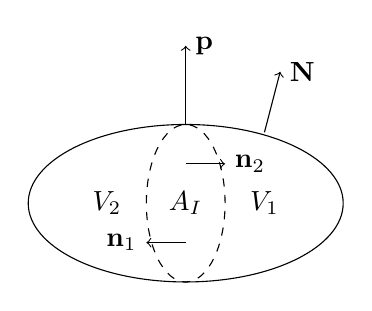
\begin{tikzpicture}
        \draw (0,0) ellipse (2 and 1);
        \draw[dashed] (0,0) ellipse (0.5 and 1)node{$A_I$};
        \draw[->](0,1)--++(0,1)node[right]{\textbf{p}}; 
        \draw[->](1,0.9)--++(0.2,0.77)node[right]{\textbf{N}}; 
        \draw[->](0,-0.5)--++(-0.5,0)node[left]{$\textbf{n}_1$}; 
        \draw[->](0,0.5)--++(0.5,0)node[right]{$\textbf{n}_2$}; 
        \draw (1,0)node{$V_1$};
        \draw (-1,0)node{$V_2$};
    \end{tikzpicture}
    \caption{Scheme of an arbitrary material control volume.   }
\end{figure}

Let $f^0$  be an arbitrary quantity to be conserved inside the non-material volume $\omega$. 
Then $\bm\Phi^0$ refer to the non-convective flux of $f^0$. 
Then $s^0$ refer to source term  related to  $f^0$. 
Then, for an arbitrary control volume we have, 
\begin{equation*}
    \ddt \int_{V} f^0 dV 
    = 
    \int_{V} s^0 dV 
    + \int_{\partial V} \mathbf{\Phi}^0 \cdot \textbf{N} dS,
\end{equation*}
where $\textbf{N}$ is the normal of the control volume. 
Any quantities defined in $V_k$ will be noted with a subscript $_k$ and those who are defined at the interface with $_I$. 
Therefore, if we decompose any quantity such as $f^0 = \sum_k f_k^0 \chi_k + f_I^0 \delta_I$ we obtain, 
\begin{multline*}
    \sum_k\left[\ddt \int_{V_k} f_k^0 dV 
    - \int_{V_k} s_k^0 dV 
    - \int_{A_k} \mathbf{\Phi}_k^0 \cdot \textbf{N} dS
    \right]
    + \ddt \int_{A_I} f_I^0 dS 
    - \int_{A_I} s_I^0 dS 
    - \int_{C} \mathbf{\Phi}_I^0 \cdot \textbf{p} dC 
    = 0
\end{multline*}
Using the Reynolds transport theorem on volume integral yields,
\begin{align*}
    \ddt \int_{V_k} f_k^0 dV 
    &= \int_{V_k} \pddt f_k^0 dV 
    + \int_{A_I \cup A_k} f_k^0 \textbf{u} \cdot \textbf{n}_k dS\\
    &= \int_{V_k} \left[
        \pddt f_k^0  + \div (f_k^0 \textbf{u}_k^0) 
    \right]dV 
    + \int_{A_I} f_k^0 (\textbf{u}_I^0 - \textbf{u}_k^0) \cdot \textbf{n}_k dS\\
\end{align*}
where $\textbf{n}_k$ is the normal of the interface $A_I$ on the outward direction of the $k$ phase. 

The second term is integrated only over $A_I$ as it is the interface between both phase and not the one of the control volume. 
Using the Ledbiz rule for integration on surface yields, 
\begin{align*}
    \ddt \int_{A_I} f_I^0 dS 
    &= \int_{A_I} \left[
        \pddt f_I^0  + \divI (f_I^0 \textbf{u}_I^0) 
    \right]dS
\end{align*}

Regarding the non-convective integrals, by using the divergence theorem we can write\citep{nadim1996concise}, 
\begin{align*}
    \int_{A_k} \mathbf{\Phi}_k^0\cdot \textbf{n}_k dS
    = \int_{V_k} \div\mathbf{\Phi}_k^0 dV
    - \int_{A_I} \mathbf{\Phi}_k^0\cdot \textbf{n}_k dS. 
\end{align*}
The last term can also be re-written with the divergence theorem \citet{nadim1996concise},
\begin{align*}
    \int_{C} \mathbf{\Phi}_I^0\cdot \textbf{p} dC 
    = \int_{A_I} \divI \mathbf{\Phi}_I^0 dS
    - \int_{A_I} \mathbf{\Phi}_I^0 \cdot \textbf{n} \div \textbf{n} dS
\end{align*}
Note that whether it is $\textbf{n}_1$ or $\textbf{n}_2$ the second term on the left conserve the same sign. 

Taking in account these reformulations, we can re-write the integral balance previously exposed by, 
\begin{align*}
    \sum_k \int_{V_k}{\left[
        \pddt f_k^0
        + \div (f_k^0\textbf{u}_k^0 - \bm\Phi_k^0)
        - s_k^0
    \right]}\\
    + \sum_k\int_{A_I}{\left[
        f_k^0(\textbf{u}_I^0 - \textbf{u}_k^0)
        + \bm\Phi_k^0
    \right]\cdot \textbf{n}_k}
    + \int_{A_I}{\left[
        \pddt f_I^0 
        + \divI (f_I^0 \textbf{u}_I - \bm\Phi_I^0)
        + \bm\Phi_I^0 \cdot \textbf{n} \div \textbf{n}
    \right]} =0 
\end{align*}

Every integral of volume must be balanced independently of the surface integral. 
This means that we can separate this equation into two, 
\begin{equation*}
    \pddt f_k  
    + \div (f_k \textbf{u}_k - \mathbf{\Phi}_k) 
    =s_k. 
\end{equation*}
\begin{equation}
    \pddt f_I  
    + \divI (f_I \textbf{u}_I -\mathbf{\Phi}_I)
    + \mathbf{\Phi}_I \cdot \textbf{n} \div \textbf{n}
    = 
    + s_I
    - \sum_k \left[
    f_k (\textbf{u}_I - \textbf{u}_k)
    + \mathbf{\Phi}_k
    \right] \cdot \textbf{n}_k. 
    \label{ap:eq:dt_f_I}
\end{equation}
These equations are valid in $\Omega_k(t)$ and $\Sigma(t)$ for volume and surface quantity, respectively. 

Now let's reformulate the third term of the surface balance equation. 
Let $\textbf{F}$ be an arbitrary surface quantity. 
It can be split into two part such as, 
\begin{equation*}
    \textbf{F} 
    = \textbf{F} \cdot \textbf{n}\textbf{n}
    + (\textbf{I} - \textbf{nn})  \cdot \textbf{F}
    = \textbf{F}_\bot + \textbf{F}_{||}.
\end{equation*}
Injecting this decomposition inside the Gauss theorem on an arbitrary control volume it can be shown that, 
\begin{equation*}
    \int_{S} \divI \textbf{F}dS
    = 
    \int_{S} \left[\divI \textbf{F}_{||} 
    + \textbf{F} \cdot \textbf{n} \div\textbf{n}
    \right]dS
\end{equation*}
Consequently, we have the following relation,
\begin{equation*}
    \int_{A_I} \divI \bm\Phi_I^0dS
    = 
    \int_{A_I} \left[\divI \bm\Phi_{I||}^0
    + \bm\Phi_I^0 \cdot \textbf{n} \div\textbf{n}
    \right]dS
\end{equation*}

By taking in account this relation it is easy to take or not the normal components of a vector to the interface within the balance equaitons. 
For example, we can write either, 
\begin{equation}
    \pddt f_I  
    + \divI (f_I \textbf{u}^I_{||} -\mathbf{\Phi}^I_{||})
    + f_I \textbf{u}_I \cdot \textbf{n} \div \textbf{n}
    - s_I
    = 
    - \sum_k \left[
    f_k (\textbf{u}_I - \textbf{u}_k)
    + \mathbf{\Phi}_k
    \right] \cdot \textbf{n}_k 
    \label{ap:eq:dt_f_I2}
\end{equation}
Or 
\begin{equation}
    \pddt f_I  
    + \divI (f_I \textbf{u}^I -\mathbf{\Phi}^I_{||})
    - s_I
    = 
    - \sum_k \left[
    f_k (\textbf{u}_I - \textbf{u}_k)
    + \mathbf{\Phi}_k
    \right] \cdot \textbf{n}_k 
    \label{ap:eq:dt_f_I2}
\end{equation}
where we have changed the flux term formulation. 



\section{Topological equations}
There is two Topological equaitons one for $\chi_k$ and an other for $\delta_I$.
First, we recall the relations related to the phase indicator function, 
\begin{equation}
    \frac{\partial}{\partial t} \chi_k
    + \textbf{u}_I  \grad \chi_k 
    = 0, \;\;\;\;\text{and}\;\;\;\; 
    \grad \chi_k 
    = - \delta_I \textbf{n}_k.
    \label{ap:eq:phase_properties}
\end{equation}
Now the surface indicator function transport equation can be obtained using the Leibniz rule for differentiation,  
\begin{equation*}
    \ddt \int_{A_I} dS
    = \int_{A_I} \grad_I \cdot \textbf{u}_I dS,
\end{equation*}
Those integrals can be re rewritten as, 
\begin{equation*}
    \ddt \int_{V} \delta_I dV
    = \int_{V} \delta_I \grad_I \cdot \textbf{u}_I dV.
\end{equation*}
Then using the Reynolds transport term for fixed material volume yields,
\begin{equation*}
    \pddt \delta_I
    + \grad \cdot (\delta_I \textbf{u}_I)
    = \delta_I \grad_I \cdot \textbf{u}_I. 
\end{equation*}
This equation can also be takes the form 
\begin{equation}
    \pddt \delta_I
    + \grad \cdot (\delta_I \textbf{u}_I\cdot \textbf{n}\textbf{n})
    = \delta_I \textbf{u}_I \cdot \textbf{n}\grad \cdot \textbf{n}. 
    \label{ap:eq:dt_delta_I}
\end{equation}
Also, it can be useful to derive an expression for the gradient of the $\delta_I$ function. 
To do so we take the gradient of \ref{ap:eq:phase_properties} yielding, 
\begin{equation*}
    \grad\delta_I 
    = \grad( - \textbf{n}_k \cdot \grad \chi_k)
    = \grad\textbf{n}_k \cdot \textbf{n}_k \delta_I
    + \grad(\textbf{n}_k \delta_I) \cdot \textbf{n}_k 
\end{equation*}
Note that the first term on the LHS vanish

\section{\textit{One-fluid} and \textit{two-fluid} formulations}
In this appendix we derive the \textit{two-fluid} and \textit{one-fluid} formulation of a generalized conservation equation, namely,
\begin{equation}
    \frac{\partial}{\partial t} f_k
    = \grad \cdot (\bm{\Phi}_k - f_k\textbf{u}_k)
    + \textbf{S}_k.
    \label{ap:eq:global_balance}
\end{equation}
Then we derive the phase averaged and global averaged equation of this general equation of conservation. 

We can derive the \textit{two-fluid} formulation by multiplying \ref{ap:eq:global_balance} by the phase indicator function \ref{eq:phase_indicator}. 
It yields, 
\begin{equation*}
    \frac{\partial}{\partial t} (\chi_k f_k)
    = \grad \cdot (\chi_k \bm{\Phi}_k - \chi_k f_k \textbf{u}_k)
    + \chi_k \textbf{S}_k.
    + f_k \frac{\partial}{\partial t} \chi_k
    + \left(
        f_k \textbf{u}_k 
        - \bm{\Phi}_k
    \right) \cdot \grad \chi_k
    % \label{ap:eq:global_balance}
\end{equation*}
where we have included the phase function $\chi_k$ into the derivative operators. 
Now, using the \ref{ap:eq:phase_properties} we get, 
\begin{equation}
    \frac{\partial}{\partial t} (\chi_k f_k)
    = \grad \cdot (\chi_k \bm{\Phi}_k - \chi_k f_k \textbf{u}_k)
    + \chi_k \textbf{S}_k
    + \left[
        \bm{\Phi}_k 
        + f_k 
        \left(
            \textbf{u}_I
            - \textbf{u}_k
        \right) 
    \right]
    \cdot \textbf{n}_k \delta_I 
    \label{ap:eq:two-fluid_global}
\end{equation}
where the last term is the interfacial source term, such as the drag force if $f_k$ is the momentum or the mass transfer if $f_k$ is the density. 
In this equation note that all quantities are factor of the phase indicator function $\chi_k$. 
So we transport $\chi_k f_k$ which is field quantity defined over the whole domain. 
Thus, \ref{ap:eq:two-fluid_global} is valid over the entire domain.   

Now, we define the jump condition across the interface or the surface transport equation as the sum of the interfacial term on each phase $k$. 
It can be obtained using  the transport of surface \ref{ap:eq:dt_f_I2}.
Indeed, multiplying \ref{ap:eq:dt_f_I2} by $\delta_I$ gives, 
\begin{equation}
    \pddt (f_I\delta_I)  
    = 
    + \grad \cdot (\delta_I \mathbf{\Phi}^I_{||} - \delta_I f_I \textbf{u}^I)
    +\textbf{S}_I \delta_I
    - \sum_k \left[
    f_k (\textbf{u}_I - \textbf{u}_k)
    + \mathbf{\Phi}_k
    \right] \cdot \textbf{n}_k \delta_I
    \label{ap:eq:general_jump}
\end{equation}
\tb{
    Note that the first term on the RHS is the parallele component of $\mathbf{\Phi}$ thus it must be reformulated as, 
    
}

Now, let's derive the \textit{one-fluid} formulation of the general conservation law.
To do so we sum on all phases \ref{ap:eq:two-fluid_global} plus the interface. 
Besides, we define any quantities $q$ such as, $q = \sum_k \chi_k q_k + \delta_I q_I$.
Then it is trivial to show that, 
\begin{equation}
    \frac{\partial}{\partial t} f
    = \grad \cdot (\bm{\Phi} - f \textbf{u})
    + \textbf{S}
    \label{ap:eq:one-fluid_global}
\end{equation}
which is the \textit{one-fluid} formulation. 

The volume average of \ref{ap:eq:two-fluid_global} is then straight forward, by using the definition of the averaged operator, we get, 
\begin{equation*}
    \frac{\partial}{\partial t} (\phi_k\kavg{f})
    = \grad \cdot \left(
        \phi_k \kavg{\bm{\Phi} - f \textbf{u}}
    \right)
    + \phi_k \kavg{\textbf{S}}
    + a_I \Iavg{
        \bm{\Phi}_k \cdot \textbf{n}_k
        + f_k 
        \left(
            \textbf{u}_I
            - \textbf{u}_k
        \right) \cdot \textbf{n}_k
    } 
\end{equation*}
Similarly, the bulk average can be obtained by averaging \ref{ap:eq:one-fluid_global} yielding, 
\begin{equation*}
    \frac{\partial}{\partial t} \avg{f}
    = \grad \cdot \avg{\bm{\Phi} - f \textbf{u}}
    + \avg{\textbf{S}}
    % + a_I\avg{\textbf{J}_I},
    \label{ap:eq:avg_global}
\end{equation*}
\section{Derivation of the point velocity}
Consider a particle of center of mass $\textbf{y}_\alpha$ defined such as
\begin{equation*}
    m_\alpha \textbf{y}_\alpha
    = \int_{V_\alpha} \rho_k \textbf{y}_k dV,
\end{equation*}
its velocity can be solely the derivation of $\textbf{y}_\alpha$ whitin time.
Yielding, 
\begin{align*}
    \ddt \textbf{y}_\alpha (t)
    &=
    \ddt \left(
        \frac{1}{m_\alpha} \int_{V_\alpha} \rho_k \textbf{y}_k dV
    \right)\\
    &= \frac{1}{m_\alpha}
    \ddt 
    \left(
        \int_{V_\alpha} \rho_k \textbf{y} dV
    \right)
    - \frac{1}{m_\alpha^2} \ddt \int_{V_\alpha} \rho_k dV \int_{V_\alpha} \rho_k \textbf{y}_k dV
    \\
    &= \frac{1}{m_\alpha}\int_{V_\alpha} \left[
        \pddt (\rho_k \textbf{y}) + \grad \cdot\left(\rho_k \textbf{y}\textbf{u}_k\right) dV 
    \right]\\
    &+ \frac{1}{m_\alpha}\int_{S_\alpha} \textbf{y} M_k d S
    -  \frac{1}{m_\alpha^2} \int_{S_\alpha} M_k dS  \int_{V_\alpha} \rho_k \textbf{y}_k dV
    \\
    &= \frac{1}{m_\alpha}\int_{V_\alpha} \textbf{y} \left[
    \pddt (\rho_k) + \grad \cdot\left(\rho_k \textbf{u}_k\right) dV 
    \right]dV
    + \frac{1}{m_\alpha}\int_{V_\alpha} \rho_k  \textbf{u}_k  \cdot \grad \textbf{y} dV \\
    &+ \frac{1}{m_\alpha}\int_{S_\alpha} \textbf{y}_k M_k d S
    - \frac{1}{m_\alpha}  \textbf{y}_\alpha \int_{S_\alpha} M_k dS
\end{align*}
By considering the mass conservation \ref{eq:single-fluid_mass} for the first term,  noticing that $\grad \textbf{y} = \textbf{I}$ where $\textbf{I}$ is the identity tensor for the second term and introducing \textbf{r} in the third term gives, we get the following relation,
\begin{equation*}
    \textbf{u}_\alpha
    = \frac{1}{m_\alpha} \left(
        \textbf{p}_\alpha
        +  \int_{S_\alpha} \textbf{r} M_k dS
    \right)
    % = \frac{1}{m_\alpha}  \left(
    %     \textbf{p}_\alpha
    % - \int_{V_\alpha} \rho_k \textbf{w} dV
    % \right)
\end{equation*}

\section{Derivation of the surface transport equations for Lagrangian particles}

By making use of the Leibniz rule together with \ref{ap:eq:dt_f_I} it can be shown that for any surface quantity $f_I$ we have, 
\begin{align*}
    \ddt \int_{S_\alpha} f_I dS
    &= \int_{S_\alpha} \pddt f_I 
    + \grad_I \cdot (\textbf{u}_If_I) dS\\
    &= \int_{S_\alpha} \left(
        \grad_I \cdot \mathbf{\Phi}_{||}^I
        + \textbf{S}_I
    \right) dS\\
    & - \sum_k \int_{S_\alpha} \left[
        f_k (\textbf{u}_I - \textbf{u}_k)
        + \mathbf{\Phi}_k
    \right] \cdot \textbf{n}_k
    dS
\end{align*}
Then remark that if $\mathbf{\Phi} = \sigma (\textbf{I}-\textbf{nn})$.
Then, 
\begin{equation*}
    \int_S \grad_I \cdot \left[\sigma (\textbf{I} - \textbf{nn})\right]dS 
    =
    \int_S  \grad_I \sigma dS 
    + \int_S \sigma \kappa \textbf{n}dS 
    = 0
\end{equation*}

Using the Gauss theorem for closed surface it can be shown easily that the first term on the RHS can be reformulated, leaving with, 
\begin{align}
    \ddt \int_{S_\alpha} f_I dS
    = \int_{S_\alpha} \left[
        \textbf{S}_I 
        - \kappa \mathbf{\Phi}_{||}^I\cdot \textbf{n} 
    \right]dS
    - \sum_k \int_{S_\alpha} \left[
        f_k (\textbf{u}_I - \textbf{u}_k)
        + \mathbf{\Phi}_k
    \right] \cdot \textbf{n}_k
    dS
\end{align}
In this equation we can see that $\mathbf{\Phi}_I$ plays no role at all. 

Now let's derive the first moment of a surface quantity, namely $f_I \textbf{r}$. 
\begin{align*}
    \ddt \int_{S_\alpha} f_I \textbf{r} dS
    &= \int_{S_\alpha} \textbf{r}\left[
        \pddt f_I 
        + \grad_I \cdot (\textbf{u}_If_I) 
    \right]dS
    + \int_{S_\alpha}
    f_I \left[
        \pddt \textbf{r} + \textbf{u}_I \cdot \grad_I \textbf{r}
    \right]
    dS\\
\end{align*}
Using \ref{ap:eq:dt_f_I} on the first term of the RHS and the relation $\grad_I \textbf{r} = (\textbf{I} - \textbf{nn})$ gives, 
\begin{align*}
    \ddt \int_{S_\alpha} f_I \textbf{r} dS
    &= \int_{S_\alpha} \textbf{r}\left[
        \grad_I \cdot \mathbf{\Phi}_I
        - \Phi_I\cdot\textbf{n}\grad\textbf{n}
        + \textbf{S}_I
    \right] dS\\
    & - \sum_k \int_{S_\alpha}\textbf{r} \left[
        f_k (\textbf{u}_I - \textbf{u}_k)
        + \mathbf{\Phi}_k
    \right] \cdot \textbf{n}_k
    dS\\
    &+ \int_{S_\alpha}
    f_I (\textbf{u}^I_{||} - \textbf{u}_\alpha)
    dS\\
\end{align*}
Using the Gauss theorem for closed surface on the first term on the RHS, this equation can be simplified to, 
\begin{align}
    \ddt \int_{S_\alpha} f_I \textbf{r} dS
    &= \int_{S_\alpha} \left(
        \textbf{S}_I\textbf{r}
        - \mathbf{\Phi}_{||}^I
    \right) dS
    + \int_{S_\alpha}
    f_I \textbf{w}_I
    dS\nonumber\\
    & - \sum_k \int_{S_\alpha}\textbf{r} \left[
        f_k (\textbf{u}_I - \textbf{u}_k)
        + \mathbf{\Phi}_k
    \right] \cdot \textbf{n}_k
    dS
    \label{ap:eq:dt_r_f_I}
\end{align}
where $\textbf{w}_{I||} = \textbf{u}_{I||} - \textbf{u}_\alpha$. 
In the jump condition of the first moment it is now evident that $\mathbf{\Phi}^I_{||}$ is relevant. 

As an example, if $f_I$ were to be the momentum of the surface, then $\mathbf{\Phi}_{||}^I = \sigma (\textbf{I} - \textbf{nn})$. 
Thus, we can express the integrals as, 
\begin{equation*}
    \int_{S_\alpha}\mathbf{\Phi}_{||}^IdS
    =\int_{S_\alpha} \sigma (\textbf{I} - \textbf{nn}) dS
    =\int_{S_\alpha} \grad_I \cdot (\sigma \textbf{r}) dS
    =\int_{S_\alpha} \sigma \textbf{r} (\grad\cdot\textbf{n}) \textbf{n} dS
\end{equation*} 
where we used the Gauss theorem on closed surface for the first term. 
In this last expression we recognize the last term as begin the first moment of the surface tension force. 




\section{Decomposition of the particular energy balance.}
This section is a detailed derivation of the energy equation for a whole fluid particle, namely,
\begin{equation*}
    \label{ap:eq:E_alpha_dt}
    \ddt E_\alpha 
    % = \ddt \int_{V_\alpha} \rho_k E_k dV
    = \int_{V_\alpha} \textbf{b}_k \cdot \textbf{u}_k dV
    + \int_{S_\alpha} \left[
        (\textbf{T}\cdot \textbf{u} 
    - \textbf{q})\cdot\textbf{n}_k 
    + M_k E_k 
    + \textbf{f}_I \cdot \textbf{u}_I 
    \right]dS, 
\end{equation*}
Since we can decompose the velocity fields of a particle following $\textbf{u}_k = \textbf{u}_\alpha + \textbf{w}$ it is then possible to rewrite the total energy, 
Yielding, 
\begin{multline*}
    \int_{V_\alpha} \rho_k E_k dV
    = \int_{V_\alpha} \rho_k e_k dV
    + \frac{1}{2} \int_{V_\alpha} \rho_k \textbf{u}_\alpha\cdot\textbf{u}_\alpha dV\\
    + \int_{V_\alpha} \rho_k \textbf{u}_\alpha\cdot\textbf{w} dV
    + \frac{1}{2} \int_{V_\alpha} \rho_k \textbf{w}\cdot\textbf{w} dV
\end{multline*}
by applying the relation \ref{eq:M_alpha_dt} on the second term, it is possible to show that,
\begin{equation*}
    E_\alpha
    = \int_{V_\alpha} \rho_k e_k dV
    + \frac{1}{2} \textbf{u}_\alpha\cdot\textbf{u}_\alpha  m_\alpha
    + \textbf{u}_\alpha\cdot \int_{V_\alpha} \rho_k \textbf{w} dV
    + \frac{1}{2} \int_{V_\alpha} \rho_k \textbf{w}\cdot\textbf{w} dV.
\end{equation*}
We clearly see that the energy can be decomposed into internal and kinetic energy. 
We define the integrated internal energy of the particle by $e_\alpha = \int_{V_\alpha} = \rho_k e_k dV$.
It is the straight forward (using \ref{eq:one-fuild_internal_energy}) to show that, 
\begin{equation*}
    \ddt e_\alpha
    = \int_{V_\alpha} \textbf{T}:\grad\textbf{u}_k dV
    + \int_{S_\alpha} \left(
        e_k M_k
        - \textbf{q}_k \cdot \textbf{n}_k
    \right) dS.
\end{equation*}
Similarly, the kinetic energy equation for a whole fluid particle can be obtained deriving the local kinetic energy ,namely,
\begin{equation*}
    \ddt \int_{V_\alpha} \rho_k \frac{u_k^2}{2} dV
    = \int_{V_\alpha}\textbf{u}_k \cdot  \left(
        \textbf{b}_k
        + \grad \cdot \textbf{T}_k
    \right)dV
    + \int_{S_\alpha} \frac{u_k^2}{2} M_k dS.
\end{equation*}
Using the velocity decomposition one can deduce, 
\begin{multline}
    \frac{1}{2} \ddt \left(
        m_\alpha \textbf{u}_\alpha \cdot \textbf{u}_\alpha
        + 2\textbf{u}_\alpha \cdot \int_{V_\alpha}  \rho_k \textbf{w}_k dV
        + \int_{V_\alpha} \rho_k \textbf{w}_k \cdot \textbf{w}_k dV
    \right)\\
    =  \textbf{u}_\alpha \left[
        \cdot\int_{V_\alpha} \textbf{b}_k dV
        +  \int_{S_\alpha} \left(
            \textbf{T}_k \cdot \textbf{n}_k
            + \frac{1}{2} \textbf{u}_\alpha M_k 
            + \textbf{w}_k M_k 
        \right)dS
    \right]\\
    + \int_{V_\alpha} \left(
        \textbf{w}_k\cdot\textbf{b}_k
        -\textbf{T}_k : \grad \textbf{w}_k
    \right)dV
    + \int_{S_\alpha} 
        \textbf{w}_k\cdot(\textbf{T}_k\cdot \textbf{n}_k)
    dS\\
    + \int_{S_\alpha} \frac{1}{2} \textbf{w}_k \cdot \textbf{w}_k M_k dS.
    \label{ap:eq:u_2_dt}
\end{multline}
Besides, taking the dot product of the centered velocity $\textbf{u}_\alpha$, with the momentum equation \ref{eq:dt_p_alpha}, gives, 
\begin{multline*}
    \frac{1}{2}\ddt (m_\alpha \textbf{u}_\alpha \cdot \textbf{u}_\alpha)
    + \textbf{u}_\alpha \cdot \ddt \int_{V_\alpha} \rho_k \textbf{w}_k dV \\
    = \textbf{u}_\alpha \cdot \int_{V_\alpha} \textbf{b}_k dV
    + \textbf{u}_\alpha \cdot \int_{S_\alpha} \left(
    \textbf{T}_k \cdot\textbf{n}_k
    +\frac{\textbf{u}_\alpha}{2} M_k
    +\textbf{w}_k M_k
    \right)dS,
\end{multline*}
We can note that the RHS of this equation correspond rigorously to the second line of \ref{ap:eq:u_2_dt}.
Therefore, taking the difference between those equations, yields the internal motion equation of an arbitrary particle, namely, 
\begin{multline*}
    \frac{1}{2}\ddt \int_{V_\alpha} \frac{\rho_k}{2} \textbf{w}_k \cdot \textbf{w}_k dV
    = \int_{V_\alpha} \left(
        \textbf{w}_k\cdot\textbf{b}_k
        -\textbf{T}_k : \grad \textbf{w}_k
    \right)dV\\
    + \int_{S_\alpha} 
        \textbf{w}_k\cdot(\textbf{T}_k\cdot \textbf{n}_k)
    dS
    + \int_{S_\alpha} \frac{1}{2} \textbf{w}_k \cdot \textbf{w}_k M_k dS.
\end{multline*}

\section{Derivation of kinetic Turbulence Evolution Equations}

The aim of this section is to derive the transport equation for the granular temperature scalar. 
Let's define the grain temperature, $T$ as such, $T =\frac{1}{2} \textbf{u}'\cdot\textbf{u}'$, where $\textbf{u}'$ is the fluctuation velocity of a given average procedure. 

\subsection{For a continuous phase}
We start this derivation for the continuous phase $k$, so that $\textbf{u}'_k = \textbf{u}_k - \kavg{\textbf{u}}$.
We start from the averaged kinetic energy equation over the $k$ phase, namely : 
\begin{multline*}
    \frac{\rho_k}{2}\frac{\partial }{\partial t}\left(
        \phi_k
        \kavg{u^2}
    \right)
    +\frac{\rho_k}{2}\grad\cdot \left(
        \phi_k
        \kavg{u^2\textbf{u}}
    \right)
    =
    \grad\cdot\left(
        \phi_k
        \kavg{\textbf{u}\cdot \textbf{T}}
    \right)
    +\phi_k\kavg{\textbf{u}\cdot\textbf{b} - \textbf{T}: \grad\textbf{u}}\\
    +a_I \Iavg{
        (\textbf{T}_k\cdot\textbf{u}_k)\cdot\textbf{n}_k
        + \frac{u^2_k}{2} M_k}.
\end{multline*}
Breaking down the LHS of this equation times $\frac{2}{\rho_k}$, yields,
\begin{align*}
    &\frac{\partial }{\partial t}\left(
        \phi_k
        \kavg{u^2}
    \right)
    +
    \grad\cdot \left(
        \phi_k
        \kavg{u^2\textbf{u}}
    \right)\\
    &=
    \phi_k\frac{\partial }{\partial t}\kavg{u^2}
    +\kavg{u^2}\frac{\partial }{\partial t}\phi_k
    +\grad\cdot \left(
        \phi_k
        \kavg{u^2}\kavg{\textbf{u}}
        +\phi_k
        \kavg{u^2\textbf{u}'}
    \right)\\
    &=
    \phi_k
    \left[
        \frac{\partial }{\partial t}\kavg{u^2}
        + 
        \kavg{\textbf{u}}
        \cdot\grad 
        \kavg{u^2}
    \right]
    +\kavg{u^2} \left[
        \frac{\partial }{\partial t}\phi_k
        + \grad\cdot \left(
            \phi_k
            \kavg{\textbf{u}}
        \right)
    \right]\\
    &+ \grad\cdot \left(
        2\phi_k
        \kavg{\textbf{u}}\cdot\kavg{\textbf{u'}\textbf{u'}} + \phi_k \kavg{T \textbf{u'}}
    \right)
\end{align*}
where we used $\kavg{u^2} = (\kavg{u})^2 + T$. 
By using the averaged mass conservation \ref{eq:avg_k_mass} times $\frac{1}{2}\kavg{u^2}$, namely, 
\begin{equation*}
    \frac{\rho_k}{2} \kavg{u^2} \pddt \phi_k 
    + \frac{\rho_k}{2} \kavg{u^2} \grad \cdot\left(\phi_k\kavg{\textbf{u}}\right)
    = \frac{a_I}{2}\kavg{u^2}\Iavg{M_k},
\end{equation*}
we can rewrite the energy balance in conservative form. 
It reads as, 
\begin{multline}
    \phi_k\frac{\rho_k}{2}  \left[
        \frac{\partial }{\partial t}
        \kavg{u^2}
        +\kavg{\textbf{u}}\cdot\grad 
        \kavg{u^2}
    \right]
    =
    \grad\cdot\left(
        \phi_k
        \kavg{\textbf{u}\cdot \textbf{T}
        - \rho_k\kavg{\textbf{u}}\cdot\textbf{u'u'}
        - \frac{\rho_k}{2}T\textbf{u'}}
    \right)\\
    +\phi_k\kavg{\textbf{u}\cdot\textbf{b} - \textbf{T}: \grad\textbf{u}}
    +a_I \Iavg{
        (\textbf{T}_k\cdot\textbf{u}_k)\cdot\textbf{n}_k
        + \frac{u^2_k - \kavg{u^2}}{2} M_k}.
    \label{ap:eq:avg_k_u_2}
\end{multline}
On the other hand the momentum equation reads as, 
\begin{multline*}
    \rho_k\pddt (\phi_k\kavg{\textbf{u}}) 
    + \rho_k\grad\cdot(\phi_k\kavg{\textbf{u}}\kavg{\textbf{u}})\\
    = \grad\cdot\left[
        \phi_k \kavg{\textbf{T}
        - \rho_k \textbf{u'u'}}
    \right]
    +\phi_k\kavg{\textbf{b}}
    + a_I\Iavg{M_k \textbf{u}_k +\textbf{n}_k\cdot\textbf{T}_k},
\end{multline*}
using the mass balance times $\kavg{\textbf{u}}$, we can write the momentum equation as, 
\begin{multline*}
    \rho_k \phi_k \left[
        \pddt \kavg{\textbf{u}}
        + \kavg{\textbf{u}}\cdot\grad\kavg{\textbf{u}}
    \right]\\
    = \grad\cdot\left[
        \phi_k \kavg{\textbf{T}
        - \rho_k \textbf{u'u'}}
    \right]
    +\phi_k\kavg{\textbf{b}}
    + a_I\Iavg{M_k \left(\textbf{u}_k - \kavg{\textbf{u}}\right) +\textbf{n}_k\cdot\textbf{T}_k}.
\end{multline*}
Then taking the dot product of this equation with $\kavg{\textbf{u}}$ gives, 
\begin{multline}
    \phi_k\frac{\rho_k}{2}  \left[
        \pddt (\kavg{u})^2
        + \kavg{\textbf{u}}\cdot\grad(\kavg{u})^2
    \right]\\
    = \grad\cdot\left[
        \phi_k \kavg{\textbf{u}}\cdot\kavg{\textbf{T}
        - \rho_k  \textbf{u'u'}}
    \right]
    +\phi_k\kavg{\rho_k \textbf{u'u'} - \textbf{T}}:\grad
         \kavg{\textbf{u}}\\
    +\phi_k\kavg{\textbf{u}}\cdot\kavg{\textbf{b}}
    + a_I\Iavg{M_k \left(\textbf{u}_k\cdot\kavg{\textbf{u}} 
    - (\kavg{u})^2\right) +\textbf{n}_k\cdot(\kavg{\textbf{u}}\cdot\textbf{T}_k)}.
    \label{ap:eq:avg_k_u_u}
\end{multline}
Finally, we can obtain the transport equation of $T$ by subtracting \ref{ap:eq:avg_k_u_2} with \ref{ap:eq:avg_k_u_u}. 
Yielding the following equation, 
\begin{multline}
    \phi_k\rho_k  \left[
        \frac{\partial }{\partial t}
        \kavg{T}
        +\kavg{\textbf{u}}\cdot\grad 
        \kavg{T}
    \right]\\
    =
    \grad\cdot\left(
        \phi_k
        \kavg{\textbf{u'}\cdot \textbf{T'}
        - \rho_k T\textbf{u'}}
    \right)
    +\phi_k\kavg{\rho_k \textbf{u'u'}}:\grad
         \kavg{\textbf{u}}\\
    +\phi_k\kavg{\textbf{u'}\cdot\textbf{b'} + \textbf{T'}: (\grad\textbf{u})'}
    +a_I \Iavg{
        (\textbf{T}_k'\cdot\textbf{u}'_k)\cdot\textbf{n}_k
        + T M_k}.
    \label{ap:eq:avg_k_T}
\end{multline}


\subsection*{Dispersed phase}

In the same spirit as the previous section we carry out the derivation for the transport of the kinetic turbulence evolution $T$. 
The only difference is that $T$ is now defined relative to the mean velocity of the particular phase $\pavg{u}$.  
From the previous section we know that we can write the energy equation under the following form, 
\begin{multline*}
    \frac{1}{2}\ddt (m_\alpha u^2_\alpha)
    + \textbf{u}_\alpha \cdot \ddt \int_{V_\alpha} \rho_k \textbf{w}_k dV 
    = \textbf{u}_\alpha \cdot \int_{V_\alpha} \textbf{b}_k dV\\
    + \textbf{u}_\alpha \cdot \int_{S_\alpha} \left[
    \textbf{T}_k \cdot\textbf{n}_k
    +\frac{\textbf{u}_\alpha}{2} M_k
    +\textbf{w}_k M_k
    \right]dS.
\end{multline*}
Applying the particular average operator yields the averaged point of mass kinetic energy equation, 
\begin{multline*}
    \frac{1}{2}\pddt   \left(\pavg{m_\alpha} \pnavg{u^2_\alpha}\right)
    + \frac{1}{2}\grad \cdot \left(\pavg{m_\alpha} \pnavg{u^2_\alpha \textbf{u}_\alpha}\right) 
    = \pavg{\textbf{u}_\alpha \cdot \int_{V_\alpha} \textbf{b}_k dV}\\
    - \frac{1}{2}\pddt \left(\pavg{m_\alpha'(u_\alpha^2)'}\right)
    - \frac{1}{2}\grad\cdot\left(\pavg{m_\alpha' (u_\alpha^2 \textbf{u}_\alpha)'}\right)\\
    - \pavg{\textbf{u}_\alpha \cdot \ddt \int_{V_\alpha} \rho_k \textbf{w}_k dV} 
    + \pavg{\textbf{u}_\alpha \cdot \int_{S_\alpha} \left[
    \textbf{T}_k \cdot\textbf{n}_k
    +\frac{\textbf{u}_\alpha}{2} M_k
    +\textbf{w}_k M_k
    \right]dS}.
\end{multline*}
From this step, we can carry out the same decomposition as the previous section for the RHS/2. 
Namely, 
\begin{multline*}
    \frac{\partial }{\partial t}\left(
        \pavg{m_\alpha}
        \pnavg{u^2_\alpha}
    \right)+
    \grad\cdot \left(
        \pavg{m_\alpha}
        \pnavg{u^2_\alpha\textbf{u}_\alpha}
    \right) \\
    =
    \pavg{m_\alpha}
    \left[
        \frac{\partial }{\partial t}\pnavg{u^2_\alpha}
        + 
        \pnavg{\textbf{u}_\alpha}
        \cdot\grad 
        \pnavg{u^2_\alpha}
    \right]
    +\pnavg{u^2_\alpha} \left[
        \frac{\partial }{\partial t}\pavg{m_\alpha}
        + \grad\cdot \left(
            \pavg{m_\alpha}
            \pnavg{\textbf{u}_\alpha}
        \right)
    \right]\\
    + \grad\cdot \left(
        2\pavg{m_\alpha}
        \pnavg{\textbf{u}_\alpha}\cdot\pnavg{\textbf{u'}\textbf{u'}} 
        + \pavg{m_\alpha} \pnavg{T \textbf{u'}}
    \right)
\end{multline*}
As we can observe the possible polydispersity of the flow, add supplementary terms linked to the fluctuation of the mass, $m_\alpha'$.
The energy equations in the conservative form then reads as, 
\begin{multline*}
    \frac{\pavg{m_\alpha}}{2}
    \left[
        \frac{\partial }{\partial t}\pnavg{u^2_\alpha}
        + 
        \pnavg{\textbf{u}_\alpha}
        \cdot\grad 
        \pnavg{u^2_\alpha}
    \right]
    = \pavg{\textbf{u}_\alpha \cdot \int_{V_\alpha} \textbf{b}_k dV} + \grad \cdot \textbf{L}\\
    - \pavg{\textbf{u}_\alpha \cdot \ddt \int_{V_\alpha} \rho_k \textbf{w}_k dV} 
    - \pavg{u_\alpha^2}\pnavg{\int_{S_\alpha} M_k d S}\\
    + \pavg{\textbf{u}_\alpha \cdot \int_{S_\alpha} \left[
    \textbf{T}_k \cdot\textbf{n}_k
    +\frac{\textbf{u}_\alpha}{2} M_k
    +\textbf{w}_k M_k
    \right]dS},
\end{multline*}
where \textbf{L} represent all the fluctuation terms derived in the two previous equations. 

Now let's look at the particular averaged momentum equation. 
Using similar decomposition as in the previous part,
and by using the decomposition of the momentum, $\textbf{p}_\alpha = m_\alpha \textbf{u}_\alpha + \int_{V_\alpha} \textbf{w}_k dV$, the equation aforesaid reads as, 
\begin{multline*}
    \pavg{m_\alpha} \left[
        \pddt \pnavg{\textbf{u}_\alpha}
        + \pnavg{\textbf{u}_\alpha}\cdot\grad\pnavg{\textbf{u}_\alpha}
    \right]
    = \pavg{\int_{V_\alpha} \textbf{b}_k dV}
    + \grad \cdot \textbf{R}\\
    - \pavg{\ddt \int_{V_\alpha} \rho_k \textbf{w}_k dV} 
    + \pavg{\int_{S_\alpha} \left[\textbf{T}_k + \rho_k \textbf{u}_k (\textbf{u}_I-\textbf{u}_k) \right] \cdot \textbf{n}_k d S}
\end{multline*}
where \textbf{R} is the term that gather all the fluctuation terms. 
Multiplying, this equation by $\pnavg{\textbf{u}_\alpha}$ and taking the difference with the energy equation yielding, 
\begin{multline*}
    \frac{\pavg{m_\alpha}}{2}
    \left[
        \frac{\partial }{\partial t}\pnavg{T_\alpha}
        + 
        \pnavg{\textbf{u}_\alpha}
        \cdot\grad 
        \pnavg{T_\alpha}
    \right]
    = \pavg{\textbf{u}_\alpha' \cdot \left(\int_{V_\alpha} \textbf{b}_k dV\right)'} 
    + \grad \cdot \left(\textbf{L}-\textbf{R}\right)\\
    - \pavg{\textbf{u}_\alpha' \cdot \left(\ddt \int_{V_\alpha} \rho_k \textbf{w}_k dV\right)'} \\
    - \pavg{T_\alpha}\pnavg{\int_{S_\alpha} M_k d S}
    + \pavg{\textbf{u}_\alpha \cdot \int_{S_\alpha} \left[
    \textbf{T}_k \cdot\textbf{n}_k
    +\frac{\textbf{u}_\alpha}{2} M_k
    +\textbf{w}_k M_k
    \right]dS},
\end{multline*}
% \chapter{Equivalence between volume average and weighted average for Lagrangian poly-disperse particles}
\label{ap:equivalence}
As mentioned in \ref{chap:avg} the velocity fields $\left<\bm{u}\right>^L_\gamma$ is needed in \ref{eq:PBM_QBMM}.
While, with the particular-average, \ref{eq:classic_hybrid_momentum_c}, we solve for $\left<\bm{u}\right>^p$.
Also, in \ref{eq:classic_hybrid_momentum_c} we have assumed an even distribution of particles size where this is clearly not the case. 
In the following we show the equivalence between the two averaged quantities and the correctness of the uniformity assumption. 
This appendix aim to prove rigorously the link between the population balance model and the particular-average equation.
The strategy is to derive \ref{eq:classic_hybrid_momentum_p} from Liouville equation following the method of \citet{curtiss1956kinetic} and \citet[chapter~7]{rao2008introduction}.
This way we show an equivalence by identification between the quantities mentioned above.

Let's consider the Boltzmann equation for a distribution $P(\textbf{x},\mathscr{C})$.
The distribution must remain physical, thus it must respect $\lim_{\mathscr{C} \rightarrow \partial\mathscr{C}} = 0$, where $\partial \mathscr{C}$ correspond to the boundary of the domain of definition of each component of $\mathscr{C}$. 
It yields, 
\begin{equation}
    \label{eq:Liouville}
    \pddt P(\textbf{x},\mathscr{C})
    + \bm{\nabla} \cdot \left(\textbf{u} P(\textbf{x},\mathscr{C})\right)
    + \nablab_\mathscr{C} \cdot \left(\frac{d\mathscr{C}}{dt} P(\textbf{x},\mathscr{C})\right) 
    = \Psi
\end{equation}
Now let's consider a function $f(\mathscr{C},t)$ which represent any physical quantity function of the internal coordinate and the time. 
Multiplying \ref{eq:Liouville} by the function, $q_\alpha$, and integrating over all the internal coordinates yields Maxwell equation,
\begin{equation}
    \int q_\alpha \pddt P d\mathscr{C}
    + \int q_\alpha \nablab \cdot \left(\textbf{u} P\right)d\mathscr{C}
    + \int q_\alpha \nablab_\mathscr{C} \cdot \left(\frac{d\mathscr{C}}{dt} P\right) d\mathscr{C} = \int q_\alpha \Psi d\mathscr{C}.
\end{equation}
The first two terms derivative can be swapped with the integral since they are not function of $\mathscr{C}$.
Then, we make use of the divergence theorem on the third term, 
yielding,
\begin{multline}
    \pddt \int q_\alpha  P d\mathscr{C}
    + \nablab \cdot\int q_\alpha \left(\textbf{u} P\right)d\mathscr{C} 
    % + \int_{\partial \lambda} \nablab_\mathscr{C} \cdot \left(f \textbf{u}_\lambda P\right) d\partial\mathscr{C} 
    = \int q_\alpha \Psi d\mathscr{C},
    +\int \left(\frac{d\mathscr{C}}{dt} P\right) \cdot \nablab_\mathscr{C} f  d\mathscr{C} 
    \label{eq:inttt}
\end{multline}
The second integral on RHS has been derived using the divergence theorem and considering that the distributions $P$ vanish near its boundaries. 
After applying the average operator \ref{eq:inttt} reads as,
\begin{equation}
    \pddt \left( n \avg{q_\alpha}\right)
    + \bm{\nabla} \cdot \left(n \avg{\textbf{u} q_\alpha}\right)
    = n \avg{\Psi q_\alpha}
    + n  \avg{\frac{d\mathscr{C}}{dt} \cdot \nablab_\mathscr{C} q_\alpha}
    \label{ap:eq:maxwell}
\end{equation}
Note that up to now we have made no assumption on the shape of $P$ and on the nature of the internal coordinates $\mathscr{C}$. 
Nevertheless, only the number of particles  $n$, appear in \ref{ap:eq:maxwell}.
At this point of the development we must specify the nature of the internal coordinates.
Thus, in the next section we investigate different situation. 
In this context the scalar $\Psi$ represent the source term due to 3 things. 
The coalescence and break-up phenomena, and the inter particular collision. 
The source term can be thus expressed under this form \citep{rao2008introduction,curtiss1956kinetic},  
\begin{equation*}
    \Psi(\mathscr{C}) = B(\mathscr{C}) + D(\mathscr{C}) + \Pi(\mathscr{C}) + \nabla \cdot \Theta(\mathscr{C})
\end{equation*}
where $B$ is the birth term, $D$ the death term, $\Pi$ the collision source term, and $\Theta$ the collision flux. 

\section{Point mass particles}
We start by considering only point of mass particles. 
Therefore, we consider only the momentum of the particles $\textbf{p}_\alpha$ and the volume $V_\alpha$ as an internal coordinate.
Thus, \ref{ap:eq:maxwell} yields,
\begin{equation}
    \pddt \left( n \avg{q_\alpha}\right)
    + \bm{\nabla} \cdot \left(n \avg{q_\alpha \textbf{u}_\alpha}\right)
    - n  \avg{\frac{\partial V_\alpha}{\partial t} \cdot \frac{\partial q_\alpha}{\partial V_\alpha}}
    - n  \avg{\frac{\partial \textbf{p}_\alpha}{\partial t} \cdot \frac{\partial q_\alpha}{\partial \textbf{p}_\alpha}}
    = n \avg{\Psi q_\alpha},
\end{equation}
From this equation we can recover the conservation equations of the particular phase by replacing $q_\alpha$ by the right quantity. 
Consider, $f = 1$, for example, we get, 
\begin{equation}
    \pddt n
    + \nablab \cdot \left(n \avg{\textbf{u}_\alpha}\right)
    = n\avg{\Psi}
\end{equation}
which is the conservation of the number density of the particles. 
Where the right-hand side is to coalesce and break up kernel.
Similarly, the mass balance equation can be obtained with $f = V_\alpha \rho_d$, yielding,
\begin{equation}
    \pddt (n\avg{m_\alpha})
    + \bm{\nabla} \cdot \left(n \avg{\textbf{u}_\alpha m_\alpha}\right)
    =
    n  \avg{\int_{S_\alpha} M_d dS},
\end{equation}
where we have use \ref{eq:dt_m_alpha} to make appear the mass transfer term. 
Notice that the source term is null since coalescence and break-up conserve the mass. 
Again, for the momentum conservation equation we set $f = \textbf{p}_\alpha$.
\begin{equation}
    \pddt \left( n \avg{\textbf{p}_\alpha}\right)
    + \nablab \cdot \left(n \avg{\textbf{u}_\alpha \textbf{p}_\alpha}\right)
    =  \nabla \cdot \Theta
    + n  \avg{\frac{\partial \textbf{p}_\alpha}{\partial t}}
\end{equation}
where $B$, $D$ and $\Pi$ cancel out since they doesn't change the momentum of the phase. 
Nevertheless, notice that the collision flux term stay \citep{rao2008introduction}.
Using, the momentum balance for a single particle \ref{eq:dt_p_alpha}, we can simplify the last term yielding, 
\begin{multline*}
    \pddt \left( n \avg{\textbf{p}_\alpha}\right)
    + \bm{\nabla} \cdot \left(n \avg{\textbf{u}_\alpha \textbf{p}_\alpha }\right)\\
    = 
    \nabla \cdot \Theta
    + n\avg{\int_{V_\alpha} \textbf{b}_k dV}
    + \avg{\int_{S_\alpha} \left(
    \textbf{T}_k\cdot\textbf{n}_k
    - M_k \textbf{u}_k
    \right)dS},
\end{multline*}
The system of equation obtained here is equivalent to \ref{eq:avg_p_momentum}, but with an additional source $\Theta$ terms representing the particle stress.

We can also set $f = \textbf{u}_\alpha$ instead of $\textbf{p}_\alpha$ and consider only $\textbf{u}_\alpha$ as an internal coordinate.
Then by using \ref{eq:u_alpha_dt} we directly have, 
\begin{multline*}
    \pddt \left( n \avg{\textbf{u}_\alpha}\right)
    + \bm{\nabla} \cdot \left(n \avg{\textbf{u}_\alpha \textbf{u}_\alpha }\right)
    = 
    \nabla \cdot \Theta
    + n\avg{\frac{1}{m_\alpha}\int_{V_\alpha} \textbf{b}_k dV} \\
    + \avg{\frac{1}{m_\alpha}\int_{S_\alpha} \left(
    \textbf{T}_k\cdot\textbf{n}_k
    - M_k \textbf{w}_k
    \right)dS}
    + \avg{\frac{1}{m_\alpha} \ddt \int_{S_\alpha} 
        \textbf{r} M_k dS},
\end{multline*}

% \section{Higher order description of the particles}
% In the previous section we only considered the center of mass velocity.
% Here we consider also the first order moment of inertia and momentum.
% Therefore, we consider the following quantities as internal coordinate,
% the momentum $\textbf{p}_\alpha$, the moment of momentum $\mathcal{P}_\alpha$ and the moment of inertia $\mathcal{G}$.
% In the following we will adopt indices notation to be more rigorous. 
% Besides, we will neglect all terms related to the mass transfer.
% \ref{ap:eq:maxwell} now reads as, 
% \begin{multline*}
%     \pddt \left( n \avg{q_\alpha}\right)
%     + \frac{\partial}{\partial x_i} \left(n \avg{\textbf{u}_\alpha q_\alpha}\right) 
%     = n \left<Jf\right>^\lambda.\\
%     + n  \left<\frac{d p^\alpha_i}{dt} \frac{\partial q_\alpha}{\partial p_i} \right>^{\lambda} 
%     + n  \left<\frac{d\mathcal{G}^\alpha_{ij}}{dt} \frac{\partial q_\alpha}{\partial\mathcal{G}_{ij}}\right>^{\lambda} 
%     + n  \left<\frac{d\mathcal{P}^\alpha_{ij}}{dt} \frac{\partial q_\alpha}{\partial\mathcal{P}_{ij}}\right>^{\lambda} 
% \end{multline*}
% Now, we can apply the same process as earlier to get the conservation equations.
% For $f = \mathcal{G}_{ij}^\alpha$ we get,
% \begin{equation*}
%     \pddt \left( n \left<\mathcal{G}_{ij}\right>^\lambda\right)
%     + \frac{\partial}{\partial x_k} \cdot \left(n \left<\mathcal{G}_{ij} u_k^\alpha \right>^\lambda\right)
%     = n \left<J \mathcal{G}_{ij}\right>^\lambda.
%     + n  \left<\mathcal{S}_\alpha\right>^{\lambda} 
% \end{equation*}
% where we have use \ref{eq:Gorderl}, with $\mathcal{S} = \mathcal{P} + \mathcal{P}^T$ ($^T$ being the transpose operator). 
% As one can notice we recover the particular averaged equation for the transport of $\mathcal{G}$.
% Besides, we assumed that $J$ does not cancel since it might not conserve the shape of particle. 
% Now, setting $f = \mathcal{P}_{ij}$ and using \ref{eq:momentMumdeq_\alpha} yields the moment of momentum equation,
% \begin{multline*}
%     \pddt \left( n \left<\mathcal{P}\right>^\lambda\right)
%     + \frac{\partial}{\partial x_i} \left(n \left<\mathcal{P} u_i^\alpha\right>^\lambda\right) 
%     = n \left<J\mathcal{P}\right>^\lambda \\
%     + \lavg{M_{ij}^\alpha}
%     - \lavg{\int_{V_\alpha} \sigma_{ij}dV}
%     + \lavg{\int_{V_\alpha} \rho_d u_i w_j dV}.
% \end{multline*}
% Again we kept the source term $J$, as we have no information on its nature while considering the moment of momentum and shape tensor. 
% As proven in \ref{ap:cinematic} we could derive additional equations for the higher order of inertia and momentum. 

% \section{Alternative derivation of the momentum equation}

% In this section we consider the following internal coordinate, the center of mass velocity $\bm{u}^\alpha$, the moment of inertia $\mathcal{G}$ and the volume $V_\alpha$.
% We would like to empathize that the center of mass velocity isn't rigorously equivalent to the moment $\textbf{p}_\alpha$ (see \ref{ap:cinematic}). 
% Indeed, the latter can be expressed as a Taylor expansion at the center of the particle. 
% Therefore, it is interesting to consider the derivation of the momentum equation using those internal coordinates.
% The global conservation equation now reads as,
% \begin{equation*}
%     \pddt \left( n \avg{q_\alpha}\right)
%     + \frac{\partial}{\partial x_i} \left(n \avg{\textbf{u}_\alpha q_\alpha}\right) 
%     - n  \left<\frac{d u^\alpha_i}{dt} \frac{\partial q_\alpha}{\partial u_i} \right>^{\lambda} 
%     - n  \left<\frac{d V_\alpha}{dt} \frac{\partial q_\alpha}{\partial V}\right>^{\lambda} 
%     - n  \left<\frac{d \mathcal{G}^\alpha_{ij}}{dt} \frac{\partial q_\alpha}{\partial \mathcal{G}_{ij}} \right>^{\lambda} 
%     = n \left<Jf\right>^\lambda.
% \end{equation*}
% According to \ref{ap:cinematic} we can express the linear momentum as $p^\alpha_j = V_\alpha u_j^\alpha + \frac{1}{2} \mathcal{G}_{kl}  K^\alpha_{jkl}+\ldots$, with $K^\alpha_{jkl} = \frac{\partial u_j^\alpha}{\partial y_k\partial y_l}|_\alpha$, where we neglected the third or above order terms. 
% Then, setting $f = p^\alpha_i$ gives, 
% \begin{multline*}
%     \pddt \left( n \left<V_\alpha u_j^\alpha + \frac{1}{2} \mathcal{G}_{kl}  K^\alpha_{jkl}\right>^\lambda\right)
%     + \frac{\partial}{\partial x_i} \left(n \left<
%         \left(V_\alpha u_j^\alpha 
%         + \frac{1}{2} \mathcal{G}_{kl}  K^\alpha_{jkl}\right) u_i^\alpha
%     \right>^\lambda\right) \\
%     + \frac{1}{2} n  \left<\frac{d\mathcal{G}_{kl}  K^\alpha_{jkl}}{dt}\right>^{\lambda} 
%     - \frac{1}{2} n  \left<\frac{d \mathcal{G}^\alpha_{kl}}{dt} K^\alpha_{jkl} \right>^{\lambda} 
%     = n \left<Jf\right>^\lambda
%     + \lavg{\bm{q_\alpha}_\alpha}
%     +\lavg{\bm{b}_{ext}}.
% \end{multline*}
% Since the averaging operator is linear, we can group the derivative yielding, 
% \begin{multline*}
%     \pddt \left( n \left<V_\alpha u_j^\alpha + \frac{1}{2} \mathcal{G}_{kl}  K^\alpha_{jkl}\right>^\lambda\right)
%     + \frac{\partial}{\partial x_i} \left(n \left<
%         \left(V_\alpha u_j^\alpha 
%         + \frac{1}{2} \mathcal{G}_{kl}  K^\alpha_{jkl}\right) u_i^\alpha
%     \right>^\lambda\right) \\
%     + \frac{1}{2} n  \left<\frac{d K^\alpha_{jkl}}{dt}\mathcal{G}_{kl}\right>^{\lambda} 
%     = n \left<Jf\right>^\lambda
%     + \lavg{\bm{q_\alpha}_\alpha}
%     +\lavg{\bm{b}_{ext}}.
% \end{multline*}


% \chapter{Proof on kinematic, shape, external forces and moments relations on deformable particle.}
\label{ap:cinematic}

    % \begin{align}
%     \phi\left<\bm{u}\right>^d 
%     &= n/\rho_d\left<\bm{p}_\alpha\right>^p
%     + \sum_{q=1}^\infty \left[\frac{(-1)^q}{q!} \prod^q_{i=1}\bm{\nabla} (n\left< \bm{Q}_\alpha^q\right>^p)\right]\\
%     \label{eq:exp}
% \end{align}
\tb{
\section{On the particles shape tensors for general to specific cases.}

All along the derivation of the averaged equations for the hybrid model we see appear this tensor : $\bm{\mathcal{G}_\alpha}^n = \int_{V_\alpha} \left(\bm{\bm{r}_\alpha}\right)^n dV$. 
In this Appendix we wish to give more physical sense to this tensor by taking the example of simple cases.
First, let's start with some basics.
For any shape the $0^{th}$ order of this tensor is the volume of the particle, it reads, $\bm{\mathcal{G}_\alpha}^0 = \int_{V_\alpha} dV = V_\alpha$.
For any particles the first order tensor $\bm{\mathcal{G}_\alpha}^0$ is always null, indeed by using the definition of  $\bm{r}_\alpha$ and $\bm{y}_\alpha$  it yields the following relation,
\begin{equation}
    \bm{\mathcal{G}_\alpha}^l
    = \int_{V_\alpha} \bm{r}_\alpha^n dV 
    = \int_{V_\alpha} \bm{y} dV - \bm{y}_\alpha \int  dV .
    = V_\alpha \bm{y}_\alpha - \bm{y}_\alpha V_\alpha 
    = 0.
\end{equation}
Then, in order to understand the meaning of the higher order tensor it is useful to think in terms of central moments and probability density function used in statistical theories. 
Therefore, the integral : $\int_{V_\alpha} \bm{r}_\alpha dV$, is equivalent to, 
\begin{equation}
    \mathcal{G}^n 
    = V_\alpha\int \bm{r}_\alpha^n f_\alpha(\bm{y}) d\bm{y},
\end{equation}
where $\bm{r}_\alpha = \bm{y}_\alpha -\bm{y}$, and $f_\alpha$ is a probability density function defined as such,
\begin{equation}
    f_\alpha(\bm{y}) = \left\{
        \begin{tabular}{cc}
        $1/V_\alpha \text{  if  }$ &$\bm{y}  \in V_\alpha$\\
        $0 \text{  if  }$ &$\bm{y} \notin  V_\alpha$
    \end{tabular}
    \right..
\end{equation}
Now we see clearly that $\mathcal{G}^n$ is the $n^{th}$ centered moment of the distribution of $f_\alpha$. 
Therefore, it follows that,
the first moment is the mean, i.e $\bm{y}_\alpha$. 
The second moment is variance, i.e. the spreading of the distribution computed by $\mathcal{G}^2$. 
The third moment is the skewness, it measures the asymmetry of the distribution, i.e. $\mathcal{G}^3$. 
The fourth moment is the Kurtosis, it measures the heaviness of the tail of the distribution, i.e. the shape. 

Some comment of the second order shape tensor are of interest. 
Indeed, it must respect some property, 

$\frac{d}{dt}\text{det}(\mathcal{G}) = 0$

to respect the pass conservation.
\subsection{2D disc shape tensor}

\tdplotsetmaincoords{70}{110}
%
\pgfmathsetmacro{\thetavec}{48.17}
\pgfmathsetmacro{\phivec}{63.5}
%
\begin{figure}[h!]
    \centering
    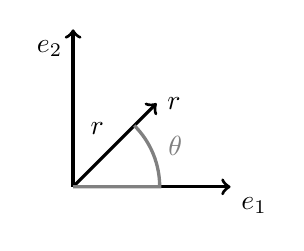
\begin{tikzpicture}[very thick]
        % \draw[fill=gray!30] (0,0)circle(1);
        \draw[->](0,0) --++ (2,0)node[below right ]{$\bm{e}_1$};
        \draw[->](0,0) --++ (0,2)node[below left ]{$\bm{e}_2$};
        \draw[->](0,0) --++ (45:1.5)node[right]{$r$}node[midway, above left]{$r$};
        \draw[gray](0,0) --++ (0:1.1)arc(0:45:1.1)node[below right]{$\;\;\;\theta$};
    \end{tikzpicture}   
	\begin{tikzpicture}[tdplot_main_coords,scale = 0.3]
		\draw[->,thick] (0,0,0) -- (6.5,0,0) node [pos=1.1] {$\bm{e}_1$};
		\draw[->,thick] (0,0,0) -- (0,6,0) node [pos=1.05] {$\bm{e}_2$};
		\draw[->,thick] (0,0,0) -- (0,0,5.5)  node [pos=1.05] {$\bm{e}_3$};   
		\tdplotsetcoord{P'}{7}{\thetavec}{\phivec}
    	\tdplotsetcoord{P''}{1}{90}{90+\phivec}
    	\tdplotsetcoord{P'''}{1}{90+\thetavec}{\phivec}
		\tdplotsetcoord{P}{6}{\thetavec}{\phivec}
		\draw[->] (0,0,0) -- (P) node [midway, above] {$r$};
		\draw[thick] (0,0,0) -- (2,4,0);
		\draw[dashed] (2,4,4) -- (2,4,0);
		\draw[dashed] (2,0,0) -- (2,4,0) node [pos=-0.1] {$x$};
		\draw[dashed] (0,4,0) -- (2,4,0) node [pos=-0.3] {$y$};
		\draw[dashed] (0,0,4) -- (2,4,4) node [pos=-0.1] {$z$};
		\draw[dashed, tdplot_main_coords] (4.47,0,0) arc (0:90:4.47);
		\node[fill=black, circle, inner sep=0.8pt] at (2,4,4) {};
		\tdplotdrawarc{(0,0,0)}{0.7}{0}{\phivec}{below}{$\phi$}
	    \tdplotsetthetaplanecoords{\phivec}
	    \tdplotdrawarc[tdplot_rotated_coords]{(0,0,0)}{0.5}{0}{\thetavec}{}{}
	    \node at (0,0.25,0.67) {$\theta$};
	\end{tikzpicture}

    \caption{Parametrization of the problem for 2D and 3D case.}
    \label{fig:schemeshpere}
\end{figure}
Now let's derive the first 4 moments for a 2D spherical particle. 
The zeroth moment reads as,
\begin{equation}
    \mathcal{G}^0 
    = \int_V  d\bm{y} 
    = \int_0^{2\pi}\int_0^{R}  d\bm{y} 
    = [\theta]_0^{2\pi}[r]_0^{R} 
    = 2\pi R
\end{equation}
where we used the notation depicted on the scheme \ref{fig:schemeshpere}.
The first moment as already mentioned is, $\mathcal{G}^1 = \int \bm{r}_\alpha dV = 0$.
Next, the second moment yields,
\begin{equation}
    (\mathcal{G}^2)_{ij}
    = \int_V r_ir_j d\bm{y} 
    = \int_0^{2\pi}\int_0^{R} r_ir_j d r dr d\theta 
    = \int_0^{R} r^3 dr \int_0^{2\pi} r_ir_j d\theta  
    = \frac{R^4}{4} \int_0^{2\pi} r_ir_j d\theta 
\end{equation}
where $\bm{r} = (\cos{\theta}, \sin{\theta})$. 
Then, 
\begin{equation}
    \mathcal{G}^2 = \frac{R^4}{4}\left[\begin{tabular}{cc}
        $\pi$&$0$\\
        $0$&$\pi$\\
    \end{tabular}
    \right].
\end{equation}
More generally the $l^{th}$ moment reads as, 
\begin{equation}
    (\mathcal{G}^l)_{i_1i_2\ldots i_l}
    = \frac{R^{l+2}}{l+2} \int_0^{2\pi} r_{i_1}r_{i_2}\ldots r_{i_l} d\theta 
\end{equation}
Then, two things can be shown. 
The first one, is that the components off-diagonal of $\mathcal{G}^l$ are null. 
The second, is that the values on the diagonal are the same. 
If we consider the sum on all indices, the product $r_{i_1}r_{i_2}\ldots r_{i_l}$ can be written $(\cos\theta+\sin\theta)^l$.
Moreover, 
\begin{equation}
    (\cos\theta+\sin\theta)^l  = \sum_{k=0}^l\binom{l}{k}\cos^k\theta\sin^{l-k}\theta
\end{equation}
Thus, the integral $\int_0^{2\pi} r_{i_1}r_{i_2}\ldots r_{i_l} d\theta$ always follows this form,
\begin{equation}
    \int_0^{2\pi} \cos^k\theta\sin^{l-k}\theta d\theta \;\;\;\forall k\leq l. 
    \label{eq:cossin}
\end{equation}
Now, we can notice that the diagonal components $I$ and $II$ (i.e. the diagonal in the sense that all the indices are the same) are equal to,
\begin{equation}
    (\mathcal{G}^l)_{I}
    = \int_0^{2\pi} \cos^l d\theta\;\;\;
    (\mathcal{G}^l)_{II}
    = \int_0^{2\pi} \sin^l d\theta  
\end{equation}
Let's develop the first term, 
\begin{align*}
    (\mathcal{G}^l)_{I}
    &= \int_0^{2\pi} \cos^l d\theta\\
    &= \frac{1}{l} \left[\cos^{l-1}\theta\sin\theta \right]_0^{2\pi} + \frac{l-1}{l} \int_0^{2\pi} \cos^{l-2} d\theta.\\
\end{align*}
The first term on the right hands side is always null. 
Indeed, $\cos$ is pair at any power of, $l-1$, and $\sin$ is odd, thus the product of the two terms is an odd function. 
Moreover, the product between $\sin$ or $\cos$ are at least $2\pi$ periodic. 
Therefore, the integral taken between $0$ and $\pi$ is null, and the relation reduce to, 
\begin{equation*}
    (\mathcal{G}^l)_{I}
    = \int_0^{2\pi} \cos^l d\theta
    =  \frac{l-1}{l} \int_0^{2\pi} \cos^{l-2} d\theta\\
    =  \frac{l-1}{l}\frac{l-3}{l-2} \int_0^{2\pi} \cos^{l-4} d\theta\\
\end{equation*}
If we keep repeating the process we eventually arrive to the smallest power. 
Which is either $0$ or $1$ if we start by, respectively a number $l$ pair and a number $l$ odd.
Therefore, we pose $l = 2q$ in the first case and $l = 2q+1$ in the second, 
\begin{equation*}
    (\mathcal{G}^{2q})_{I}
    =  \frac{2q-1}{2q}\frac{2q-3}{2q-2} \int_0^{2\pi} \cos^{2q-4}\theta d\theta\\
    =  \prod^{q-1}_{k= 0}\frac{2q-2k-1}{2q-2k} \int_0^{2\pi}  d\theta\\
    =  \prod^{q-1}_{k= 0}\frac{2q-2k-1}{2q-2k} 2\pi\\,
\end{equation*}
and,
\begin{equation*}
    (\mathcal{G}^{2q+1})_{I}
    =  \prod^{q}_{k= 0}\frac{2q-2k}{2q-2k+1} \int_0^{2\pi} \cos \theta d\theta\\
    = 0.
\end{equation*}
Similar calculation can be done for the powers of $\sin$, and it yields the same results. 
Therefore, the diagonal components of the $l^{th}$ order tensor of a disk are, 
\begin{equation}
    \mathcal{G}_{I}^l=\mathcal{G}_{II}^l = \left\{\begin{tabular}{cc}
        $\prod^{q-1}_{k= 0}\frac{2q-2k-1}{2q-2k} 2\pi $& if $l = 2q$     \\
        $0 $        & if $l = 2q+1$
    \end{tabular}\right.
    \label{eq:cosl}
\end{equation}
In fact, if we can carry out similar calculations for the integral, \ref{eq:cossin}, we find that, 
\begin{equation}
    \int_0^{2\pi} \sin^k \cos^{l-k} dV = \frac{1}{2}\frac{k-1}{l-k-1} \int_0^{2\pi} \sin^{l-2}\theta \cos^{l-k+2}\theta d\theta.
\end{equation}
Notice that taking $l = 2q$ or $l=2q+1$ leads to either $\sin^0\theta^{l-k+2q} $ or $\sin \theta^{l-k+2q+1}$ in the integral. 
Therefore, the integral of  $\sin \theta^{l-k+2q+1}$ between $0$ and $2\pi$ will ultimately cancel out. 
Therefore, we obtain the following relation in the non-null cases,
\begin{equation}
    \int_0^{2\pi} \sin^k \cos^{l-k} d\theta = \left\{\begin{tabular}{cc}
        $\prod^{q-1}_{n=0}\frac{2q-2n-1}{l-2q+2n+1} \int_0^{2\pi} \cos^{l} d\theta$& if $k = 2q$     \\
        $0 $        & if $l = 2q+1$
    \end{tabular}\right.
\end{equation}
Using \ref{eq:cosl} yields,
\begin{equation}
    \int_0^{2\pi} \sin^k \cos^{l-k} d\theta = \left\{\begin{tabular}{cc}
        $\prod^{q-1}_{n=0}\frac{2q-2n-1}{2r-2q+2n+1} \prod^{r-1}_{n= 0}\frac{2r-2n-1}{2r-2n} 2\pi $& if $k = 2q$ and $l = 2r$    \\
        $0$        & if $k = 2q  $ and $l = 2r +1$\\
        $0$        & if $k = 2q+1$ and $l = 2r$\\
        $0$        & if $k = 2q+1$ and $l = 2r +1$
    \end{tabular}\right.
\end{equation}
The remaining question is now, how to link the indexes of the tensor to the value of $k$.
If we consider a tensor of order $2$ it is easy to say that, 
\begin{equation}
    \mathcal{G}_{ij} = \delta_{ij} \frac{R^4}{4}\pi. 
\end{equation} 
For a $4^{th}$ order tensor it is given by, 
\begin{equation}
    \mathcal{G}_{ijkl} = (\delta_{ij}\delta_{kl} + \delta_{ik}\delta_{lj}) \frac{R^6}{8} \pi
\end{equation} 
we can deduce the pattern for the higher order tensor. 
Indeed, the non-null terms can be defined by the sum of all the possible product of $\delta$.
It can be shown that for a tensor of order $l$ the number of combination of $\delta$ is $n= 1+(l/2-1)l/2$.
}
\section{3D sphere shape tensor}
For spherical particles, it is possible to carry out similar calculation using spherical coordinate. 
Nevertheless, it is more convenient to use tensor calculation for this matter. 
Using spherical coordinates it follows,
\begin{align*}
    \mathcal{G}_{i_1i_2\ldots i_l}^l 
    &= \rho_d \int_{V_\alpha} \prod^l_{m=1}r^\alpha_{i_m} dV\\
    &= \rho_d \int_0^R r^{l+2} dr  
      \int_{S_\alpha} \prod^l_{m=1}r^\alpha_{i_m} dS\\
    &=\rho_d \frac{R^{l+3}}{l+3}
      \int_{S_\alpha}  n_{i_l} \prod^{l-1}_{m=1} r^\alpha_{i_m} dS\\
    &=\rho_d \frac{R^{l+3}}{l+3}
      \int_{V_\alpha}  \partial_{i_l} \left(\prod^{l-1}_{m=1} r^\alpha_{i_m}\right) dV\\
    &=\rho_d \frac{R^{l+3}}{l+3}\sum_{k=1}^{l-1} \delta_{i_l i_k}
      \int_{V_\alpha}  \prod^{l-1}_{\substack{m=1\\ m\neq k}} r^\alpha_{i_m} dV\\
\end{align*}
where we recognize the $l-2$ order shape tensor in the last expression. 
By carrying the same calculation for this tensor we can compute the original $l^{th}$ order shape tensor in a recursive manner. 
We notice that all odds order shape tensor will reduce to a sum of $\int r^\alpha dV$ which is null. 
To conclude, the  $l^{th}$ shape tensor of any spherical particles is null for any odd order. 
Moreover, for even order tensor we can notice that the components non-null are carried by Kronecker symbols which is the expression of isotropy of the particle. 
Indeed, repeating the previous formula leads to this expression,
\begin{align*}
    \mathcal{G}_{i_1i_2\ldots i_l}^l 
    &=\rho_d \frac{R^{l+3}}{l+3}\sum_{a=1}^{l-1} \delta_{i_l i_a}
      \int_{V_\alpha}  \prod^{l-1}_{\substack{m=1\\ m\neq a}} r^\alpha_{i_m} dV\\
    &=\rho_d \frac{R^{l+3}}{l+3}
    \frac{R^{l+1}}{l+1}\sum_{a=1}^{l-1} \delta_{i_l i_a}
    \sum_{\substack{b=1\\ b\neq a}}^{l-2} \delta_{i_{l-1} i_b}
      \int_{V_\alpha}  \prod^{l-2}_{\substack{m=1\\ m\neq a\\ m\neq b}} r^\alpha_{i_m} dV\\
    &=\rho_d \frac{R^{l+3}}{l+3}
    \frac{R^{l+1}}{l+1} 
    \ldots
    \frac{R^3}{3}
    V_\alpha
    \delta_{i_l i_a}
    \delta_{i_{l-1} i_b}
    \delta_{i_{l-2} i_c}
    \ldots
    \delta_{i_2i_1},
\end{align*}
In further developments we will refer to the product of all the scalar values with the letter $A^l$. 
Therefore, 
\begin{equation}
    \mathcal{G}_{i_1i_2\ldots i_l}^l 
    = A^l V_\alpha
    \delta_{i_l i_a}
    \delta_{i_{l-1} i_b}
    \delta_{i_{l-2} i_c}
    \ldots
    \delta_{i_2i_1},
    \label{eq:shapeT}
\end{equation}
where it is implies that we sum the expression on $a$, $b$, $c\ldots$ in their respective range. 

From this formula we can derive the theoretical expression of the second order shape tensor. 
\begin{equation*}
    \mathcal{G}_{ij} 
    = \rho \int_{V_\alpha} \textbf{r} \textbf{r} dV 
    = \rho \int_0^R r^2 dr \int_{S_\alpha} \textbf{n} \textbf{n}  dS 
    = \rho \frac{R^3}{3} \int_{V_\alpha} \grad \textbf{n} dV
    = \rho \frac{R^2}{3} V_\alpha \delta_{ij}
\end{equation*}
where we have used the relation $\frac{\partial}{\partial y_i}n_j = R^{-1} \delta_{ij}$, notice that this is equivalent to the regular calculation, i.e. 
\begin{equation*}
    \mathcal{G}_{zz} 
    = \int_{V_\alpha} r^2 \cos^2{\theta} dV 
    = \int_{0}^R \int_{\phi = 0}^{2\pi} \int_{\theta = 0}^{\pi} r^4 \cos^2{\theta} \sin{\theta} drd\theta d\phi
    = \frac{4R^5}{15}\pi
\end{equation*}

POZRIKIDIS P 217 

\tb{
\subsection{Second order shape tensor for elongated particles}

Now let's consider any particles oriented along its axis of revolution $\bm{p}$. 
Any shape tensor can be expressed as $\mathcal{G}^2_{ij} = p_ip_j G_{||} + (\delta_{ij} - p_ip_j) G_{\bot}$ where $G_\bot$ and $G_{||}$ are constants value corresponding to Eigenvalues values of the shape tensor. 
For antisymmetric particles the Eigenvectors are aligned with the axis of revolution. 
Therefore, using a polar coordinates frame $(r, \theta, z)$ aligned with $\bm{p}$ yields the following formulas for the Eigenvalues of the shape tensor :
\begin{equation}
    G_{||} = \int_V z z dV \;\;\;\;\;\;
    G_{\bot} = \int_V r^2 \cos^2\theta dV.
\end{equation}
As an example let's now consider cylindrical particles of radius $R$ and aspect ratio $\chi$.
Then,
\begin{equation}
    G_{||} = \int_0^R\int_{-\chi R}^{\chi R} \int_0^{2\pi} z z r dr d\theta dz
    = \frac{2}{3}\pi R^5 \chi^3
\end{equation}
\begin{equation}
    G_{\bot} = \int_0^R\int_{-\chi R}^{\chi R} \int_0^{2\pi} r^3 \cos^2\theta dr d\theta dz
    = \frac{1}{2} \pi R^5 \chi.
\end{equation}
If we consider a 2D ellipse where the main axis are of length $a$ and $b$ we can express the shape tensor as,
\begin{equation}
    \mathcal{G}_{11}
    = \frac{\pi}{4}a^3b,
    \;\;\;\; 
    \mathcal{G}_{22}
    = \frac{\pi}{4}b^3a. 
    \label{eq:shapeellipse}
\end{equation}

}
\section{Kinematic equations for the $l^{th}$ order surface tensor.}

Here is the proof of the surface tensor derivations,
\begin{equation*}
    \ddt \int_{S_\alpha} dS 
    = \int_{S_\alpha} \grad_I \cdot \textbf{u}_I dS
\end{equation*}
\begin{equation*}
    \ddt \int_{S_\alpha} \textbf{r} dS 
    = \int_{S_\alpha} \textbf{r} \grad_I \cdot \textbf{u}_I dS
    + \int_{S_\alpha} \textbf{u}_I  \cdot (\textbf{I}-\textbf{nn}) dS
    - \textbf{u}_\alpha \int_{S_\alpha} dS
\end{equation*}
\begin{equation*}
    \ddt \int_{S_\alpha} \textbf{rr} dS 
    = \int_{S_\alpha} \textbf{rr} \grad_I \cdot \textbf{u}_I dS
    + 2 \int_{S_\alpha}\textbf{r} \textbf{u}_I  \cdot (\textbf{I}-\textbf{nn}) dS
    - \int_{S_\alpha} \textbf{u}_\alpha \textbf{r} + \textbf{r}  \textbf{u}_\alpha dS
\end{equation*}
Now we can write the derivation for an arbitrary tensor orders, using the Reynolds transport theorem it reads, 
\begin{align*}
    \ddt \int_{S_\alpha} \pri{1}{n}dS
    &= \int_{S_\alpha} \pddt \left(
        \pri{1}{n}
    \right) dS
    + \int_{S_\alpha} 
    \partial_k^I  \left(
        u^I_k \pri{1}{n}
    \right)dS \\
    &= - \sum_{e=1}^n u^\alpha_{i_e} \int_{S_\alpha} 
        \prod_{\substack{m = 1 \\m \neq e}}^{n} r_{i_m}
     dS
    + \int_{S_\alpha} u^I_k
    \partial_k^I  \left(
         \prod_{m=1}^{n} r_{i_m}
    \right)dS \\
    &+ \int_{S_\alpha} 
    \prod_{m=1}^{n} r_{i_m}
    \partial_k^I u^I_k 
    dS \\
\end{align*}
Using the definition of the surface derivative
\begin{align*}
    \ddt \int_{S_\alpha} \pri{1}{n}dS
    &= \int_{S_\alpha} 
    \prod_{\substack{m = 1 \\m \neq e}}^{n} r_{i_m}
    \partial_k^I u^I_k 
    dS 
    - \sum_{e=1}^n u^\alpha_{i_e} \int_{S_\alpha} 
    \prod_{\substack{m = 1 \\m \neq e}}^{n} r_{i_m}dS \\
    &+ \sum_{e=1}^n \int_{S_\alpha} u^I_k
    \prod_{\substack{m = 1 \\m \neq e}}^{n} r_{i_m}
    (\delta_{ki_e} - n_kn_{i_e}) dS \\
    &= \int_{S_\alpha} 
    \prod_{\substack{m = 1 \\m \neq e}}^{n} r_{i_m}
    \partial_k^I u^I_k dS 
    + \sum_{e=1}^n  \int_{S_\alpha} (w^I_{i_e} - u^I_kn_kn_{i_e}) 
    \prod_{\substack{m = 1 \\m \neq e}}^{n} r_{i_m}dS \\
\end{align*}
Thus, 
\begin{align*}
    \int_{S_\alpha} 
    \prod_{\substack{m = 1 \\m \neq e}}^{n} r_{i_m}
    \partial_k^I u^I_k dS 
    &=
    \ddt \int_{S_\alpha} \pri{1}{n}dS
    + \sum_{e=1}^n u^\alpha_{i_e} \int_{S_\alpha} 
    \prod_{\substack{m = 1 \\m \neq e}}^{n} r_{i_m}dS \\
    &+ \sum_{e=1}^n \int_{S_\alpha} u^I_k
    \prod_{\substack{m = 1 \\m \neq e}}^{n} r_{i_m}
    (n_kn_{i_e} - \delta_{ki_e}) dS \\
\end{align*}


\section{Equations for arbitrary moment of mass.}
Let consider the $l^{th}$ order shape tensor $\mathcal{G}^l_\alpha$ of a given particle $\alpha$. 
In this section we demonstrate how to take the time derivative of any tensor $\mathcal{G}^l_\alpha$. 
In this section we are going to make use of Einstein summation convention to represent the arbitrary order tensors. 
Besides, for a better understanding of the equations we use the notation $\bm{r}^\alpha$ for $\bm{r}_\alpha$ (which is the distance between the center of mass and a given point). 
The shape tensor of any order $l$ is defined by,
\begin{equation}
    \mathcal{G}_{i_1i_2\ldots i_l}^l = \rho_d \int_{V_\alpha} \prod^l_{m=1}r^\alpha_{i_m} dV,
\end{equation}
where each $i_m$ represent different indices. 
Then taking the time derivative and using \ref{eq:timetransport} gives the following relation,
\begin{multline}
    \frac{d}{dt}\mathcal{G}_{i_1i_2\ldots i_l}^l 
    = \rho_d \int_{V_\alpha} \left[ \frac{\partial}{\partial t} \left(\prod^l_{m=1}r^\alpha_{i_m}\right) 
    + \frac{\partial}{\partial y_k} \left(u_k\prod^l_{m=1}r^\alpha_{i_m}\right) \right]dV\\
    +\int_{S_\alpha} \prod^l_{m=1}r^\alpha_{i_m} \rho_d \left((u_I)_k - u_k\right) n_k^\alpha dS,
\end{multline}
where we recall that the second term is due to mass transfer and will be noted $T^l_\alpha$ for compactness. 
Using, the product rule on the derivative yields the following relation :
\begin{multline}
    \frac{d}{dt}\mathcal{G}_{i_1i_2\ldots i_l}^l 
    = \rho_d \int_{V_\alpha} \sum_{e=1}^l \left[ \prod^l_{\substack{ m=1 \\   m \neq e}}r^\alpha_{i_m} \frac{\partial}{\partial t} \left(r_{i_e}\right) 
    + \prod^l_{m=1}r^\alpha_{i_m} \frac{\partial}{\partial y_k} \left(u_k\right) 
    \right.\\
    \left.
    + u_k \frac{\partial}{\partial y_k} \left(\prod^l_{m=1}r^\alpha_{i_m}\right) \right]dV
    +T^\alpha_{i_1i_2\ldots i_l},
\end{multline}
where we can recognize the second term as the divergence of the velocity, which is null since the fluid is incompressible. 
Now, by making use of the product rule on the third term it yields,
\begin{equation}
    \frac{d}{dt}\mathcal{G}_{i_1i_2\ldots i_l}^l 
    = \rho_d \int_{V_\alpha} \sum_{e=1}^l \prod^l_{\substack{ m=1 \\   m \neq e}} r^\alpha_{i_m}\left[ \frac{\partial}{\partial t} \left(r_{i_e}\right) 
    + u_k \frac{\partial}{\partial y_k} \left(r_{i_e}\right) \right]dV
    +T^\alpha_{i_1i_2\ldots i_l},
\end{equation}
The term within the brackets can be simplified thanks to \ref{eq:momentofmomentumDev} as the fluctuation of the velocity around the center of mass noted $\bm{w}^\alpha$.
\begin{equation}
    \frac{d}{dt}\mathcal{G}_{i_1i_2\ldots i_l}^l 
    = \rho_d \sum_{e=1}^l \int_{V_\alpha}  \prod^l_{\substack{ m=1 \\   m \neq e}} r^\alpha_{i_m} w_{i_e}dV
    +T^\alpha_{i_1i_2\ldots i_l}.
\end{equation}
In the summation sign we can recognize the $(l-1)^{th}$ moment of momentum tensor. 
\begin{equation}
    \frac{d}{dt}\mathcal{G}_{i_1i_2\ldots i_l}^l 
    = \sum_{e=1}^l P^\alpha_{i_1\ldots i_e\ldots i_l}
    +T^\alpha_{i_1i_2\ldots i_l}.
\end{equation}
Each terms in the sum is just the same tensor where we have permuted the indices. 
All the possible permutations are in the sum since there is only two different vectors, i.e. $\bm{r}^\alpha$ and $\bm{w}^\alpha$, and $\bm{w}^\alpha$ takes all the places among the $\bm{r}^\alpha$.
Furthermore, the sum of all the permutations of a tensor is proportional to its symmetric part \citep{itin2022decomposition}. 
Thus, we define the $^\text{Sym}$ operator which return the symmetric part of any $l^{th}$ order tensor. 
In tensor form the previous relation is then,
\begin{equation}
    \frac{d}{dt}\mathcal{G}^l 
    = l (\bm{P}_\alpha^l)^{\text{Sym}}
    +\bm{T}^\alpha.
    \label{eq:dt_G_alpha_l}
\end{equation}
The rate of change of the shape of the particle is therefore linked directly to its own moment of momentum. 
But it does not depend on the antisymmetric part. 
Which mean that the angular momentum do not play any role in the change of the shape. 
Next, we apply the particular average to this set of equations using \ref{eq:partia}.
It yields a $l$ order equation, 
\begin{equation}
    \partial_t\left(n\left<\mathcal{G}_{i_1i_2\ldots i_l}^l\right>^p\right) 
    +\partial_k\left(n\left<u_k\mathcal{G}_{i_1i_2\ldots i_l}^l\right>^p\right) 
    = n\;l\left<(P^\alpha_{i_1\ldots i_e\ldots i_l})^\text{Sym}\right>
    +n\left<T^\alpha_{i_1i_2\ldots i_l}\right>.
\end{equation}
Then, we obtained a set of $l$ equations which describe the evolution and the transport of the averaged shape properties. 
In the following we review the meaning for each of the first orders equations. 
Besides, we neglect the mass transfer term as it is not useful for our application. 
\tb{In those equations we must add the conservation of volume condition.
Look into \citet{maffettone1998equation}}

\tb{
\subsection{Equation at the first order}
At the first order we have the following relation, 
\begin{equation}
    \frac{d}{dt}\mathcal{G}^1 
    =  \frac{\partial}{\partial t} \rho_d \int_{V_\alpha} \bm{r}_\alpha dV 
    = \rho_d \int_{V_\alpha} \bm{w}_\alpha dV
    = 0. 
\end{equation}
We recall that $\bm{r}_\alpha$ is defined such that $\int_{V_\alpha} \bm{r}_\alpha dV$ is null. 
Therefore, this relation leads to a null term. 

\subsection{Second order relation}
At the second order the relation is, 
\begin{equation}
    \frac{d}{dt}\mathcal{G}^2
    = 2 (\bm{P}_\alpha^2)^{\text{Sym}}. 
    \label{eq:dGdt}
\end{equation}
Therefore the following calculation might not make sense
Thus, the rate of change of the shape of the particle is equal to the symmetric part of the moment of momentum. 
Let's study this equation in the linear displacement hypothesis to get a more physical conclusion of the matter. 
From the previous section (\ref{eq:linear2}), and by keeping only the symmetric part of $\bm{P_\alpha}$ one can deduce, 
\begin{equation}
    \frac{d}{dt}\mathcal{G}^2
    = 2 \bm{E}_\alpha \cdot \mathcal{G}^2. 
\end{equation}
Which gives us a set of $d^2$ (where $d$ is the dimension) linear differential equations for the shape tensor, namely
\begin{equation}
    \frac{d}{dt}\mathcal{G}^2_{ij}
    = 2 E^\alpha_{ik}  \mathcal{G}^2_{kj}. 
\end{equation}


}
\section{Dynamical equations for the $l^{th}$ order momentum tensor.}
Let consider the $l^{th}$ order momentum tensor $\bm{P}^l_\alpha$ of a given particle $\alpha$. 
In this section we demonstrate how to take the time derivative of any tensor $\bm{P}^l_\alpha$. 
We are going to make use of Einstein summation convention to represent the arbitrary order tensors. 
The momentum tensor of any order $l$ is defined by,
\begin{equation}
    P_{i_1i_2\ldots i_l}^{l} = \rho_d \int_{V_\alpha} \prod^{l-1}_{m=1}r^\alpha_{i_m} u_{i_l} dV,
\end{equation}
Then taking the time derivative and using \ref{eq:timetransport} gives the following relation,
\begin{multline*}
    \frac{d}{dt}P_{i_1i_2\ldots i_l}^l 
    = \rho_d \int_{V_\alpha} \left[ \frac{\partial}{\partial t} \left(\prod^{l-1}_{m=1}r^\alpha_{i_m} u_{i_l}\right) 
    + \frac{\partial}{\partial y_k} \left(u_k\prod^{l-1}_{m=1}r^\alpha_{i_m} u_{i_l}\right) \right]dV\\
    +\int_{S_\alpha} \prod^{l-1}_{m=1}r^\alpha_{i_m} u_{i_l} \left((u_I)_k - u_k\right) n_k^\alpha dS.
\end{multline*}
The last term is the moment of momentum of mass transfer and will be referred as $(T_u^\alpha)_{i_1i_2\ldots i_l}$ 
using the product rule for the derivation of the terms inside the first integral gives, 
\begin{multline*}
    \frac{d}{dt}P_{i_1i_2\ldots i_l}^l 
    = 
    \rho_d \int_{V_\alpha} u_{i_l}\left[  \frac{\partial}{\partial t} \left(\prod^{l-1}_{m=1}r^\alpha_{i_m} \right) 
    + u_k \frac{\partial}{\partial y_k} \left(\prod^{l-1}_{m=1}r^\alpha_{i_m}\right) \right]dV\\
    +\rho_d \int_{V_\alpha}  \prod^{l-1}_{m=1}r^\alpha_{i_m} \left[ 
    \frac{\partial}{\partial t} \left(u_{i_l}\right) 
    + \frac{\partial}{\partial y_k} \left(u_k u_{i_l}\right) 
    \right]dV
    +(T_u^\alpha)_{i_1i_2\ldots i_l},
\end{multline*}
Using the same calculation as in the previous section for the first term, and using,  the development carried in \ref{chap:avg} for the second leads to, 
\begin{multline*}
    \frac{d}{dt}P_{i_1i_2\ldots i_l}^l 
    = 
    \rho_d \sum_{e=1}^{l-1} \int_{V_\alpha} u_{i_l}  \prod^{l-1}_{\substack{ m=1 \\   m \neq e}} r^\alpha_{i_m} w_{i_e}dV\\
    +\rho_d \int_{V_\alpha}  \prod^{l-1}_{m=1}r^\alpha_{i_m} \left[ 
    \partial_k \sigma_{ki_l} + b_{i_l} + f^\sigma_{i_l}   
    \right]dV
    +(T_u^\alpha)_{i_1i_2\ldots i_l}.
    \label{eq:B68}
\end{multline*}
Besides, we can derive the following relation,
\begin{multline*}
    \partial_k\left(\prod^{l-1}_{m=1}r^\alpha_{i_m}  \sigma_{ki_l}\right)
    = \prod^{l-1}_{m=1}r^\alpha_{i_m} \partial_k \sigma_{ki_l} 
    + \sigma_{ki_l} \partial_k \prod^{l-1}_{m=1}r^\alpha_{i_m}\\
    = \prod^{l-1}_{m=1}r^\alpha_{i_m} \partial_k \sigma_{ki_l} 
    + \sum^{l-1}_{e =1} \sigma_{i_ei_l} \prod^{l-1}_{\substack{m=1\\ m\neq e}}r^\alpha_{i_m}  
\end{multline*}
Therefore, term involving the divergence of the stress in \ref{eq:B68} can be rewritten as so, 
\begin{equation}
    \int_{V_\alpha} \prod^{l-1}_{m=1}r^\alpha_{i_m} \partial_k \sigma_{ki_l} dV
    =
    \int_{V_\alpha} \partial_k\left(\prod^{l-1}_{m=1}r^\alpha_{i_m}  \sigma_{ki_l}\right) dV 
    -\int_{V_\alpha} \sum^{l-1}_{e=1} \sigma_{i_ei_l}  \prod^{l-1}_{\substack{m=1\\ m\neq e}}r^\alpha_{i_m}  dV
\end{equation}
Using the divergence theorem on the first term yields,  
\begin{equation}
    \int_{V_\alpha} \prod^{l-1}_{m=1}r^\alpha_{i_m} \partial_k \sigma_{ki_l} dV
    =
    \int_{S_\alpha} \prod^{l-1}_{m=1}r^\alpha_{i_m}  \sigma_{ki_l}^fn_k dS 
    -\int_{V_\alpha} \sum^{l-1}_{e=1} \prod^{l-1}_{\substack{m=1\\ m\neq e}}r^\alpha_{i_m}  \sigma_{i_ei_l}^d dV,
\end{equation}
noticing that the first term represent the $l^h$ order of the hydrodynamic moment and the terms in brackets in \ref{eq:B68} represent the $l^{th}$ moment of the body forces and surface tension force,
\begin{multline}
    \frac{d}{dt}P_{i_1i_2\ldots i_l}^\alpha
    = 
    (M^h_\alpha)_{i_1\ldots i_l}
    +(M^\sigma_\alpha)_{i_1\ldots i_l}
    +(M^b_\alpha)_{i_1\ldots i_l}\\
    +\rho_d  \int_{V_\alpha} \sum_{e=1}^{l-1}  \prod^{l-1}_{\substack{ m=1 \\   m \neq e}} r^\alpha_{i_m} w_{i_e} u_{i_l}dV
    -\rho_d\int_{V_\alpha} \sum^{l-1}_{e=1} \prod^{l-1}_{\substack{m=1\\ m\neq e}}r^\alpha_{i_m}  \sigma_{i_ei_l}^d dV
    +(T_u^\alpha)_{i_1i_2\ldots i_l}.
    \label{eq:dt_P_order_l}
\end{multline}
Furthermore, as a consequence of the summation, the $5^{th}$ term on the right hands side is symmetric on all indices from $1$ to $l-1$.
Besides, the stress tensor is by definition symmetric on its own indices, i.e. $i_e$ and $i_l$. Therefore, this term is symmetric on all its indices and will vanish if one takes the antisymmetric part of the equation. 
By applying the decomposition of the velocity $u_i = u^\alpha_i + w_i$ we obtain a fully symmetric tensor plus the moments of the fluctuations times the mean velocity.
Knowing that it is possible to derive two distinct equations, one for the antisymmetric part and symmetric part. 
Using \ref{eq:Gorderl} the equation for the symmetric part reads as,
\begin{multline*}
    \frac{d^2}{dt^2}G_{i_1i_2\ldots i_l}^\alpha
    = 
    (S^h_\alpha)_{i_1\ldots i_l}
    +(S^\sigma_\alpha)_{i_1\ldots i_l}
    +(S^b_\alpha)_{i_1\ldots i_l}\\
    +\rho_d  \int_{V_\alpha} \sum_{e=1}^{l-1}  \prod^{l-1}_{\substack{ m=1 \\   m \neq e}} r^\alpha_{i_m} w_{i_e} u_{i_l}dV
    -\rho_d\int_{V_\alpha} \sum^{l-1}_{e=1} \prod^{l-1}_{\substack{m=1\\ m\neq e}}r^\alpha_{i_m}  \sigma_{i_ei_l}^d dV
    +(T_u^\alpha)_{i_1i_2\ldots i_l}.
\end{multline*}
Which is the equation of state of the particle shape tensor. 
And the antisymmetric part yields, 
\begin{multline*}
    \frac{d^2}{dt^2}G_{i_1i_2\ldots i_l}^\alpha
    = 
    (S^h_\alpha)_{i_1\ldots i_l}
    +(S^\sigma_\alpha)_{i_1\ldots i_l}
    +(S^b_\alpha)_{i_1\ldots i_l}\\
    +\rho_d  \int_{V_\alpha} \sum_{e=1}^{l-1}  \prod^{l-1}_{\substack{ m=1 \\   m \neq e}} r^\alpha_{i_m} w_{i_e} u_{i_l}dV
    -\rho_d\int_{V_\alpha} \sum^{l-1}_{e=1} \prod^{l-1}_{\substack{m=1\\ m\neq e}}r^\alpha_{i_m}  \sigma_{i_ei_l}^d dV
    +(T_u^\alpha)_{i_1i_2\ldots i_l}.
\end{multline*}

Anyhow, it is now possible ti apply the particular average the transport of momentum equation yielding, 
\begin{multline*}
    \partial_t\left(n\left<\mathcal{P}_{i_1i_2\ldots i_l}^\alpha\right>^p\right)
    +\partial_k\left(n\left<u_k\mathcal{P}_{i_1i_2\ldots i_l}^\alpha\right>^p\right)
    =
    \pavg{M^\alpha_{i_1\ldots i_l}}\\
    +\rho_d \pavg{ \int_{V_\alpha} \sum_{e=1}^{l-1}  \prod^{l-1}_{\substack{ m=1 \\   m \neq e}} r^\alpha_{i_m} w_{i_e} u_{i_l}dV}
    -\rho_d \pavg{\int_{V_\alpha} \sum^{l-1}_{e=1} \prod^{l-1}_{\substack{m=1\\ m\neq e}}r^\alpha_{i_m}  \sigma_{i_ei_l}^d dV}\\
    + \pavg{T^\alpha_{i_1i_2\ldots i_l}},
\end{multline*}
for the moment of momentum, were
$M^\alpha_{i_1\ldots i_l}$ is the sum of the moments due to the hydrodynamic forces, the surface tension forces and the body forces.

\subsection*{Arbitrary order moments equation}

Let's define the arbitrary moment of the tensor $f$, by, 
\begin{equation*}
    Q_{i_1\ldots i_n}
    = \int_{V_\alpha} 
    \pri{1}{n} f dV
\end{equation*}
Then,
\begin{multline*}
    \ddt Q_{i_1\ldots i_n}
    =\int_{V_\alpha} \left[ \partial_t \left(\pri{1}{n}f\right) 
    + \partial_k \left(u_k \pri{1}{n}f\right) \right]dV\\
    +\int_{S_\alpha} \pri{1}{n} f \left(u^I_k - u_k\right) n_k dS.
\end{multline*}
Using the product rule on the derivatives yields, 
\begin{multline*}
    \ddt Q_{i_1\ldots i_n}
    =\int_{V_\alpha} f \left[ \partial_t \left(\pri{1}{n}\right) 
    + u_k \partial_k \left( \pri{1}{n}\right) \right]dV\\
    +\int_{V_\alpha} \pri{1}{n} \left[ \partial_t \left(f\right) 
    +  \partial_k \left(u_k f \right) \right]dV\\
    +\int_{S_\alpha} \pri{1}{n} f \left(u^I_k - u_k\right) n_k dS.
\end{multline*}
From similar arguments as before one can easily show that, 
\begin{multline*}
    \ddt Q_{i_1\ldots i_n}
    = \sum_{e=1}^{n} \int_{V_\alpha} f  \prod^{n}_{\substack{ m=1 \\   m \neq e}} r_{i_m} w_{i_e}dV
    +\int_{V_\alpha} \pri{1}{n} \grad\cdot\mathbf{\Phi} dV\\
    + \int_{V_\alpha} \pri{1}{n} \textbf{S} dV
    +\int_{S_\alpha} \pri{1}{n} f \left(u^I_k - u_k\right) n_k dS.
\end{multline*}
The second term can be reformulated such as,
\begin{align*}
    \int_{V_\alpha} \pri{1}{n} \grad\cdot\mathbf{\Phi} dV
    &= \int_{S_\alpha} \grad \cdot \left(\pri{1}{n} \mathbf{\Phi} \right)dV
    - \int_{V_\alpha} \mathbf{\Phi} \cdot \grad \left(\pri{1}{n} \right)dV\\
    &= \int_{S_\alpha} \pri{1}{n} \mathbf{\Phi} \cdot \textbf{n}dS
    -\sum_{e=1}^{n} \int_{V_\alpha} \mathbf{\Phi}  \prod^{n}_{\substack{ m=1 \\m \neq e}} r_{i_m}  dV
\end{align*}
Including this relation into the former equation yields, 
\begin{multline*}
    \ddt Q_{i_1\ldots i_n}
    = \sum_{e=1}^{n} \int_{V_\alpha} \prod^{n}_{\substack{ m=1 \\   m \neq e}} r_{i_m} (w_{i_e}f  - \Phi)dV
    +\int_{S_\alpha} \pri{1}{n} \mathbf{\Phi} \cdot \textbf{n}dS\\
    + \int_{V_\alpha} \pri{1}{n} \textbf{S} dV
    +\int_{S_\alpha} \pri{1}{n} f \left(u^I_k - u_k\right) n_k dS.
\end{multline*}
Then it is possible from this equation to carry out a particular average but also to get the local scale equations. 
Indeed, if we consider $V_\alpha$ as being a fixed control volume the above equality can be rewritten such as, 
\begin{multline*}
    \pddt \left(\pri{1}{n}f\right)
    + \grad \cdot \left(\pri{1}{n}f \textbf{u}\right)
    = n  \pri{1}{n-1}  (w_{i_n}f  - \Phi)\\
    + \pri{1}{n} \textbf{S} 
    + \grad \cdot \left( \pri{1}{n} \mathbf{\Phi} \right)
    \label{ap:eq:dt_rrf}
\end{multline*}


\subsection{On the first hydrodynamic moment and its contribution.}

While providing closure term for the first moment the user must know which part is function of the local pressure since it is absolute. 
We recall that the first hydrodynamic moment of a particle reads as,
\begin{equation}
    (M^h_\alpha)_{ij} 
    = \int_{S_\alpha} r^\alpha_i \sigma_{jk} n_k dS.
\end{equation}
In this section we discuss the different contribution from the viscous and pressure stress to the first moment tensor by investigating the specific case of a particle in a uniform flow. 
We consider a flow where pressure can be express as the sum of a constant pressure $p_0$, a constant gradient along the $z$ coordinate, and a fluctuation part $p'$, thus $p =p_0 + f_b z + p'$ where $p'$ is the fluctuation and $f_b$ the constant gradient ($f_b = \rho_f g$ is the case of buoyant flows). 
Therefore, the stress tensor reads as, $\sigma_{jk} = -p \delta_{jk} + \mu_f (\partial_j u_k+\partial_k u_j)$.
Besides, the particles are assumed spherical, thus $r_i = n_i R$ over the surface $S_\alpha$, where $R$ is the radius. 
Injecting the previous facts in the first moment expression gives,
\begin{equation}
    (M^h_\alpha)_{ij} 
    = - p_0 \int_{S_\alpha} r_i n_j dS
    - f_b \int_{S_\alpha} r_i n_j z dS
    - \int_{S_\alpha} r_i n_j p' dS
    + \int_{S_\alpha} r_i n_k \mu_f (\partial_j u_k+\partial_k u_j) dS
    \label{eq:Fistmomentdec}
\end{equation}
The viscous and pressure fluctuation part are function of local property of the flow, 
consequently they cannot be computed theoretically. 
So, let's focus on the first and second terms in the case of spherical particles. 
Using spherical coordinate, any point, $\bm{r} = (r\sin\theta \cos\phi,\; r\sin\theta \sin\phi,\; r\cos\theta )$,
Therefore the first term can be written, 
\begin{equation}
    p_0 \int_{S_\alpha} r_i n_j dS
    = p_0 R^3 \int_{0}^{2\pi}\int_{0}^\pi n_i n_j \sin\theta d\theta d\phi.
\end{equation}
Then, we have to compute the integral of each member of the following matrix,
\begin{multline}
    p_0 R^3 \int_{0}^{2\pi}\int_{0}^\pi n_i n_j \sin\theta d\theta d\phi
    =\\
     p_0 R^3 \int_{0}^{2\pi}\int_{0}^\pi
    \left[
        \begin{matrix}
            \sin^3\theta \cos^2\phi & \sin^3\theta  \cos\phi \sin\phi
            &\cos\theta\sin^2\theta \cos\phi\\
            \sim& \sin^3\theta \sin^2\phi & \sin^2\theta \cos\theta\sin\phi \\
            \sim& \sim & \sin\theta \cos^2\theta \\
        \end{matrix}
    \right]
    d\theta d\phi,
\end{multline}
by using the separation of variable method one can compute any of these integrals and find that only the diagonal components remain, and we find that, 
\begin{equation}
    p_0 R^3 \int_{0}^{2\pi}\int_{0}^\pi n_i n_j \sin\theta d\theta d\phi
    = \frac{4}{3}  p_0 R^3 \pi \delta_{ij}.
\end{equation}
Likewise, the second term of \ref{eq:Fistmomentdec} reads as,
\begin{multline}
    f_b \int_{S_\alpha} r_i n_j z dS
    =\\
     f_b R^3 \int_{0}^{2\pi}\int_{0}^\pi
    \left[
        \begin{matrix}
            \sin^3\theta \cos\theta \cos^2\phi & \sin^3\theta \cos\theta \cos\phi \sin\phi
            &\cos^2\theta\sin^2\theta \cos\phi\\
            \sim& \sin^3\theta \cos\theta \sin^2\phi & \sin^2\theta \cos^2\theta\sin\phi \\
            \sim& \sim & \sin\theta \cos^3\theta \\
        \end{matrix}
    \right]
    d\theta d\phi,
\end{multline}
Since the function depending on $\theta$ are antisymmetric around $\pi/2$ the integrals of the diagonal term are null.
In addition, the anti-diagonal components must be null due to the anisotropy of the geometry, and they are.  
In conclusion, the absolute pressure contribute to the first moment as $ \frac{4}{3}  p_0 R^4 \pi \delta_{ij}$, and the pressure gradient do not. 
Consequently, care must be taken while computing the stresslet on DNS software since we do not want the absolute pressure to appear in the results. 


\subsection{On the first moment of the surface tension}
The aim of this part is to express the link between the first order moment of the surface tension, i.e. $\bm{M}^\sigma_\alpha$ to the shape of the particle, i.e. the shape tensor $\mathcal{G}_\alpha$.
In the moment of momentum equation we see appear the unique contribution to the surface tension on the averaged equation though the first moment of the surface tension defined as,
\begin{equation}
    (M^\sigma_\alpha)_{ij}=\int_{S_\alpha}r^\alpha_i f^\sigma_j dS
\end{equation}
using the definition of the surface forces with a constant surface tension $\sigma$ gives, 
\begin{equation}
    (M^\sigma_\alpha)_{ij}=\int_{S_\alpha}r^\alpha_i \sigma \kappa n_j dS
\end{equation}
where $\kappa = -\nabla \cdot \bm{n}$ is the curvature of the surface. 
For spherical particles $\kappa = 1/R$ where $R$ is the radius of the sphere.
Therefore, the moment over the surface of the particle reads,
\begin{align}
    (M^\sigma_\alpha)_{ij}
    &= \frac{\sigma}{R}\int_{S_\alpha}r^\alpha_i n_j dS
    = \frac{\sigma}{R}\int_{V_\alpha} \partial_j r^\alpha_i dV
    = V_\alpha \frac{\sigma}{R}  \delta_{ij}\\
    &
    = \frac{4}{3} \pi R^2 \sigma  \delta_{ij} 
    \text{ for sphere, and  } 
    \pi R \sigma  \delta_{ij} 
    \text{ for circle.} 
    )
    \label{eq:MtensionCric}
\end{align}
The moment is fully isotropic, and in the static isolated case, it clearly expresses the hydrostatic pressure due to surface force applied on a spherical particle. 

For arbitrary shaped particles it gives we need to decompose the problem in two sub-problems. 
Any geometry can be decomposed by a static sphere of radius $R_m(t)$ plus a perturbed shape which can be described with a $2\pi$ periodic function $f(t,\theta,\phi)$. 
Similarly, we can define the curvature $\kappa$ as the sum of $\kappa_1$, which is the mean curvature and $\kappa_2$ is the fluctuations from the surface of the spherical geometry. Then,
\begin{equation}
    (M^\sigma_\alpha)_{ij}
    =\int_{S_\alpha}r^\alpha_i \sigma \kappa_1 n_j dS
    +\int_{S_\alpha}r^\alpha_i \sigma \kappa_2 n_j dS\\
    = \underbrace{\frac{4}{3} \pi \sigma R_m^2(t)  \delta_{ij}}_{\text{Spherical}}
    +
    \underbrace{\int_{S_\alpha(t)}r^\alpha_i \sigma \kappa_2 n_j dS}_{\text{Deviatoric}},
\end{equation}
where we can clearly identify the spherical and deviatoric part of the moment due to surface forces,
and we empathize the dependency of the surface $S_\alpha(t)$ with time. 
Before going further it is important to notice that the deviatoric part of this tensor isn't necessarily symmetric, consequently it must appear in the torque equation.
Now we let's consider a 2D deformable ellipsoid of volume, $\pi R_m^2$, and as semi-minor axis $a(t)$ and $b(t)$. 
By exploiting the conservation of volume property we obtain the following relation, 
$a(t) = R^2_m/b(t)$. 
The coordinates an ellipse can be represented by $\bm{r} = (a(t) \cos\theta, b(t)\sin\theta)$. 
Besides, in 2D it can be shown (see \citet{tryggvason2011direct}) that the normal and curvature of the surface, respectively $\bm{n}$ and $\kappa$ can be express as,
\begin{equation}
    \bm{n} 
    = \frac{\left(b(t) \cos\theta, a(t)\sin\theta\right)}{(a^2(t)\sin^2\theta+b^2(t)\cos^2\theta)^{1/2}},
    \;\;\;\;
    \kappa
    = \frac{- R_m^2}{(a^2(t)\sin^2\theta+b^2(t)\cos^2\theta)^{3/2}}.
\end{equation}

Subsequently, we can formulate $\bm{r}$ as 
$r_i = A_{ik} n_k (a^2(t)\sin^2\theta+b^2(t)\cos^2\theta)^{1/2}$, 
where $A_{ik} =b(t)/a(t) e^1_ie^1_k+a(t)/b(t)e^2_ie^2_k$,
as well, the norm of $|\bm{r}| = (a^2(t)\cos^2\theta+b^2(t)\sin^2\theta)^{1/2}$.
We can now express the first moment of the surface tension in polar coordinate, using the relation 
$dS = (a^2(t)\sin^2\theta+b^2(t)\cos^2\theta)^{1/2}d\theta$.
\begin{equation*}
    (M_{\alpha}^\sigma)_{ij} 
    = - \sigma R_m^2 A_{ik} b(t)^{-3}\int_{0}^{2\pi}
    e_k  e_j 
    (c(t)\sin^2\theta+\cos^2\theta)^{-3/2} 
    d\theta,
\end{equation*}
where $c = b^2/a^2$, $\bm{e}$ is $\bm{n}$ times its own norm, so it can be expressed in terms of $c(t) $ as well. 
It can be demonstrated that the anti-diagonal components are antisymmetric functions, thereby, they vanish under the integration operator $\int_0^{2\pi}$. 
Nonetheless, the integral of the diagonal components are not trivial, indeed they involve elliptical integral of the first and second kind, namely $K(x)$ and $E(x)$. It reads,
\begin{equation*}
    \bm{M}_{\alpha}^\sigma
    = - \sigma R_m^2 A_{ik} \left[    
        \begin{matrix}
            b^{-1} \frac{(E(1 - c^2) - K(1 - c^2))}{c^2-1} & 0\\
            0 & a^{-1} c\frac{cK(1 - c^2) - E(1 - c^2)}{c^2-1}\\
        \end{matrix}
    \right].
\end{equation*}
In the limit of small $(c-1)$ and discarding the terms above $\mathcal{O}(c-1)^2$, the elliptic integral reads,
\begin{align*}
    (\bm{M}_{\alpha}^\sigma)_{22}
    &= - \sigma \pi R_m^2 
            a^{-1} (1 -\frac{3}{4}   (c-1)+\frac{9}{16}   (c-1)^2 )
    +O\left((c-1)^3\right)\\
    (\bm{M}_{\alpha}^\sigma)_{22}
    &= - \sigma \pi R_m^2 
            b^{-1} (1 +\frac{3}{4}   (c-1)-\frac{3}{16}   (c-1)^2)
    +O\left((c-1)^3\right)\\
    \label{eq:momentSigma}
\end{align*}
One can notice that for $a(t) = R_m$ we recover the expression for circular drop \ref{eq:MtensionCric}.
\tb{make appear the shape tensor inside}

\subsubsection*{Ellipsoid}

In indices notation,  
\begin{equation*}
    \sigma_{I,ij}^0 =\gamma\left[
    \delta_{ij} - \frac{ H_{ik} H_{jl} :  r_kr_l}{  H_{ab}  H_{ac} r_br_c} \right]
\end{equation*}
Integrating this over a surface will eventually leads to an elliptic integral due to the elliptical surface. 

If the spheroid is aligned with the principal axes $\textbf{H} = \textbf{e}_1\textbf{e}_1 / a^2(t) + (\textbf{e}_2\textbf{e}_2+ \textbf{e}_3\textbf{e}_3)/b^2(t)$.
Thus, $\textbf{H}\cdot \textbf{r} = H_{ij} r_j = {e}_{1,i}{e}_{1,j}r_j / a^2(t) + ({e}_{2,i}{e}_{2,j} + {e}_{3,i}{e}_{3,j})r_j/b^2(t) $ which gives, the vector, 
$\textbf{H}\cdot \textbf{r} = \textbf{e}_{1} x/ a^2(t) + (\textbf{e}_{2}y + \textbf{e}_{3}z)/b^2(t)  = \textbf{e}_i r_i /a_i^2$
Consequently, the second term of the last equality reads in a main axis as, 
\begin{equation*}
    \frac{ H_{ik} H_{jl} :  r_kr_l}{  H_{ab}  H_{ac} r_br_c} 
    = \textbf{e}_i \textbf{e}_j \frac{ r_i r_j /(a_i a_j)^2 }
    {\frac{z^2}{a^4}+\frac{y^2+x^2}{b^4}}
\end{equation*}
To dealt with this ellipsoid integral we may employ the following change of variable :
\begin{align*}
    x = b \sin \theta \cos \phi\\
    y = b \sin \theta \sin \phi\\
    z = a \cos \theta 
\end{align*}
with $\theta \in [0,\pi]$ and $\phi \in [0,2\pi]$. 
The point on the ellipsoid surface can then be written as $\textbf{v} = [x(\theta,\phi),y(\theta,\phi),z(\theta,\phi)]$. 
Now let's first consider the surface calculation, in our coordinate system we have, 
\begin{equation*}
    \iint_S dS
    = 
    \int_{0}^{2\pi}
    \int_{0}^{\pi}
    \left|\frac{\partial \textbf{v}}{\partial \theta} 
    \times 
    \frac{\partial \textbf{v}}{\partial \phi} \right|
    d\theta
    d\phi
\end{equation*}
The partial derivative reads, 
\begin{align*}
    \frac{\partial \textbf{v}}{\partial \theta}
    = 
    b \cos \theta \cos \phi \textbf{e}_x
    + b \cos \theta \sin \phi\textbf{e}_y
    - a \sin \theta \textbf{e}_z
    \\
    \frac{\partial \textbf{v}}{\partial \phi}
    = 
    - b \sin \theta \sin \phi \textbf{e}_x
    + b \sin \theta \cos \phi\textbf{e}_y
\end{align*}
Taking the norm of the above vector cross product yields the relation : 
$dS = \left|\frac{\partial \textbf{v}}{\partial \theta} 
\times 
\frac{\partial \textbf{v}}{\partial \phi} \right| d\theta d\phi = b \sin\theta (a^2\sin^2\theta+ b^2 \cos^2\theta)^{1/2}d\theta d\phi$. 

Injecting these coordinate into the previous integrand formula for the dyadic normal reads, 
\begin{equation*}
    \frac{ H_{ik} H_{jl} :  r_kr_l}{  H_{ab}  H_{ac} r_br_c} 
    = \textbf{e}_i \textbf{e}_j \frac{ r_i r_j /(a_i a_j)^2 }
    {\frac{1}{a^2}\cos^2 \theta+\frac{1}{b^2}\sin^2 \theta (\cos^2 \phi+ \sin^2 \phi)}
    = \textbf{e}_i \textbf{e}_j \frac{ r_i r_j}
    {\frac{(a_i a_j)^2}{a^2}\cos^2 \theta+\frac{(a_i a_j)^2}{b^2}\sin^2 \theta }
\end{equation*}
Due to symmetry consideration the crossed terms are all null thus the remaining terms to evaluate are just the diagonal terms. 
The first term of the surface stress, that we call $S_1$ is the surface energy, i.e. the surface of the ellipsoid times the surface tension coefficient $\gamma$. 
\begin{equation*}
    (S_1)_{ij} 
    = \delta_{ij} 2\pi 
    \int_0^\pi 
    b \sin\theta (a^2\sin^2\theta+ b^2 \cos^2\theta)^{1/2} d\theta 
    = 2\pi b \left[\frac{a^2}{\sqrt{b^2-a^2}} \text{asinh}\left(\frac{\sqrt{b^2-a^2}}{a}\right)+b\right]
\end{equation*} 
where $\text{asinh}$ is the Hyperbolic Arc Sine function.
Note that the surface can be reformulated as,  
\begin{equation*}
    s_\alpha
    = 2\pi b \left[\frac{a^2}{\sqrt{b^2-a^2}} \text{ln}\left(\frac{b + \sqrt{b^2-a^2}}{a}\right)+b\right]
\end{equation*} 
which is more convenient. 
This expression is consistent with the classic ex pression of an ellipsoid surface. 
Now let's compute the integral $S_{2,zz}$ it reads, 
\begin{align*}
    S_{||}
    = 
    \gamma\int_0^{2\pi}\int_0^{\pi}\left[
        \frac{\cos^2\theta}{\cos^2 \theta+\frac{a^2}{b^2}\sin^2 \theta }
    \right]
    b \sin\theta (a^2\sin^2\theta+ b^2 \cos^2\theta)^{1/2} d\theta d\phi\\
    = 
    \gamma\int_0^{2\pi}\int_0^{\pi}\left[
        \frac{\cos^2\theta}{b^2\cos^2 \theta+a^2\sin^2 \theta }
    \right]
    b^3 \sin\theta (a^2\sin^2\theta+  b^2\cos^2\theta)^{1/2} d\theta d\phi\\
    = 
    \gamma 2\pi \int_0^{\pi}
    b^3 \cos^2\theta\sin\theta (a^2\sin^2+  b^2\cos^2\theta)^{-1/2} d\theta\\
    = \gamma 2\pi  b^3\,\left({{2\,b}\over{2\,b^2-2\,a^2}}-{{a^2\,{\rm asinh}\; \left(
    {{\sqrt{b^2-a^2}}\over{a}}\right)}\over{\left(b^2-a^2\right)^{{{3
    }\over{2}}}}}\right)
\end{align*}
Now let's see for the perpendicular components, namely, 
\begin{align*}
    S_{\bot}
    = 
    b a^2\gamma\int_0^{2\pi}\sin^2\phi d\phi 
    \int_0^{\pi}
        \sin^2\theta
    \sin\theta (a^2\sin^2\theta+ b^2 \cos^2\theta)^{-1/2} d\theta \\
    = 
    b a^2\gamma \pi
    \int_0^{\pi}
    \sin^3\theta (a^2\sin^2\theta+ b^2 \cos^2\theta)^{-1/2} d\theta \\
\end{align*}

The final results is the following, 
The surface tension stress can be written in terms of the two principal axis of the ellipsoid in the laboratory reference frame with, 
\begin{equation*}
    \intS{\bm{\sigma}_I^0}
    = \frac{2}{3} s_\alpha \gamma \textbf{I} + \textbf{pp} (-2 S)  + (\textbf{I} - \textbf{pp}){S}
\end{equation*}
where the first term is the isotropic part consisting into the surface energy and the second and third terms correspond to the components of anisotropy of the surface stress, namely, 
\begin{align*}
    S
    = 
    {{\left(\pi\,a^4\,b-4\,\pi\,a^2\,b^3\right)\,\log \left({{\sqrt{b^2
    -a^2}+b}\over{a}}\right)+\sqrt{b^2-a^2}\,\left(2\,\pi\,b^4+\pi\,a^2
    \,b^2\right)}\over{\sqrt{b^2-a^2}\,\left(3\,b^2-3\,a^2\right)}}
\end{align*}
We recall that this quantity drives the stress jump at the interface. 
As it is expected this stress jump is axis symmetric around the particle main axis. 
Besides, it is maximum at the poles and minimum at the equator of the particle. 
It is then possible to compute the integral of the stress by direct integration in the reference frame of the ellipsoid principal axes. 
The exact result yields, 
\begin{equation*}
    \gamma\pSavg{\textbf{I}-\textbf{nn}}
    = \gamma \left[
        \frac{2}{3} s_\alpha \textbf{I}
        + S (\textbf{I}-\textbf{pp}) -2S\textbf{pp}
        \right]
\end{equation*}
where the first component correspond to the isotropic part of the surface stress, and the second component to the deviatoric part of the surface stress. 
Notice that the deviatoric part of this tensor is function of one unique coefficient, $S$ due to the axis symmetrical nature of the droplets. 
Exact solution can be given in terms of the small deformation parameter $e_\bot = b/r$. 
Then an approximation can be deduced for the $e -1 \ll 1$, it gives,
\begin{align*}
    s_\alpha 
    = 4\pi r^2 \left[\frac{e_\bot^2}{2} + \frac{\ln\left(\sqrt{{e_\bot^6}-1}+{e_\bot^3}\right)}{2e_\bot\sqrt{e_\bot^6-1}}\right]
    = 4 \pi r^2 + \frac{24 v }{5 r} (e_\bot-1)^2\\
    S = \frac{4}{3} \pi r^2 \left[
    \frac{\left( \frac{1}{4} - e_\bot^6\right)  \log{\left( \sqrt{e_\bot^6-1}+{e_\bot^3}\right) } }
    { e_\bot  \left( e_\bot^6- 1\right)^{3/2} }
    +  \frac{e_\bot^2\left( e_\bot^6+  \frac{1}{2}\right)}{2\left( e_\bot^6- 1\right)}  \right]
    \approx 
    \frac{8 v}{5 r}(e_\bot-1) + \frac{12 v }{35r}(e_\bot-1)^2 \ldots
\end{align*}
Regarding the expression of the surface of the spheroid, it can be noticed that the function within bracket tends to $1$ for $e=1$ leaving us with $s_\alpha = 4\pi r^2$ which is the surface of the sphere. 
Then, it slowly increases when $e$ is either superior or inferior to $1$. 

Equally, the results can be expressed in terms of the deformation parameter $e_{||} = a/r$ in which case the previous results give at the second order in $e_\bot-1$ the following expression, 
\begin{align*}
    s_\alpha 
    \approx 4 \pi r^2 + \frac{6 v }{5 r} (e_{||}-1)^2 \ldots\\
    S 
    \approx 
    - \frac{4 v}{5 r}(e_{||}-1) + \frac{24 v }{35r}(e_{||}-1)^2 \ldots
\end{align*}
Noticing that the strain tensor $\textbf{C} = (e_{||}-1) \textbf{pp} + (e_\bot-1)(\textbf{I}- \textbf{pp})$ one can finally write,
\begin{align*}
    \gamma\pSavg{\textbf{I}-\textbf{nn}}
    = \frac{\gamma v}{r} \left[
        2  + \frac{6 }{10 } (\textbf{C}:\textbf{pp})^2 + \frac{6 }{10 } [\textbf{C}:(\textbf{I}-\textbf{pp})]^2\right] \textbf{I}\\
        + \frac{\gamma v}{r} \left[ \frac{8}{5} \textbf{C}
        + \frac{12}{35}[\textbf{C}\cdot \textbf{C}- 6 (\textbf{C}:\textbf{pp})^2\textbf{pp}]
        \right]
\end{align*}
This gives the surface stress tensor up to the second order terms in accuracy. 
To our knowledge this has never been proposed. 
\subsection{Discussion on the moment of momentum equation and specific case} 
\ref{eq:momentMumdef} can be split into a symmetric part, and an antisymmetric part, the former is linked to the momentum of the rate of strain and the latter correspond to the angular momentum balance.
In the angular momentum balance equation we can notice that all the symmetric quantities vanish, i.e. $\bm{\sigma}^{\text{Anti}} = 0$ and $(\bm{uw_\alpha})^{\text{Anti}} =0$, 
Thus, it has the form, 
\begin{equation}
    \frac{d\bm{P}_\alpha^{\text{Anti}}}{dt} 
    = \bm{T}_\alpha^{h}
    + \bm{T}_\alpha^{b}
    + \bm{T}_\alpha^\sigma,
\end{equation} 
where $\bm{T}$ is the torque tensor defined as $\bm{T} = \epsilon\cdot\bm{\tau}$.
In the symmetric part of the equation none of the terms vanish, while the moment over the surface traction becomes stresslets of hydrodynamic, body and surface forces referred as respectively, $\bm{S}_\alpha^h$, $\bm{S}_\alpha^b$ and $\bm{S}_\alpha^\sigma$. 
Is, reads as, 
\begin{equation}
    \frac{d\bm{P}_\alpha^{\text{Sym}}}{dt} 
    + \int_{V_\alpha} \bm{\sigma} dV
    = \bm{S}_\alpha^{h}
    + \bm{S}_\alpha^{b}
    + \bm{S}_\alpha^\sigma
    + \rho_d\int_{V_\alpha} (\bm{u}\bm{w}_\alpha+\bm{w}_\alpha\bm{u}) dV.
\end{equation} 
Now let's consider the specific case of an isolated droplet $\alpha$ immersed in an inert fluid ($\bm{u} = 0$).
Thus, all the terms cancel, except the stress in the fluid phase which reduce to $\sigma_{ij}^f = -p^f_0\delta_{ij}$,
the stress in the dispersed phase $\sigma_{ij}^d = -p^d_0 \delta_{ij}$,
and the first moment of the surface tension $(M^\sigma_\alpha)_{ij} =\sigma \int_{S_\alpha} \kappa r^\alpha_i n_j dS$.
Consequently, we can write the following equality, 
\begin{equation}
    \bm{M}^\sigma_\alpha 
    + \bm{M}^h_\alpha 
    - \int \sigma^d dV
    = 0,
\end{equation}
after expanding each term we get, 
\begin{equation}
    \sigma \int_{S_\alpha} \kappa r^\alpha_i  n_j  dS
    + \int_{S_\alpha}  r_i^\alpha \sigma_{jk}^f n_k dS
    - \int \sigma_{ij}^d dV
    = 0,
\end{equation}
\begin{equation}
    \sigma \int_{S_\alpha} n_i  n_j  dS
    - R p^f_0 \int_{S_\alpha} n_i n_j dS
    + p^d_0 \int\delta_{ij} dV
    = 0.
\end{equation}
Considering spherical coordinate and particle geometry, noticing that $\kappa$ is constant,   
and applying the expression computed in the previous section for the integral of $n_in_j$ we can show that : 
\begin{equation}
    \kappa \sigma \delta_{ij}= \Delta P \delta_{ij},
\end{equation}
where $\Delta P = p^f_0 - p^d_0$. 
Consequently, the moment of momentum equation is equivalent to the Laplace equation in this case. 

Now let's consider the case of a 2D deformable ellipse with constant volume. 
Besides, we consider non-viscous flow, so that $\mu_d = \mu_f = 0$.  
Thus, the droplets will be subject to pressure forces and surface tension forces only.  
In this specific case, the geometry is not in its state of equilibrium, i.e. a sphere, so the moment of momentum will not cancel.  
Since we do not know the velocity fields a priori, we make use of \ref{eq:dGdt} to express the moment of momentum as the derivative of the shape tensor.
Hence, we must discard the antisymmetric part of the equation. 
Accordingly, the moment of momentum equilibrium reads as, 
\begin{equation}
    \frac{d^2}{dt^2}\int_{V_\alpha} r_ir_j dV
    =
    \sigma \int_{S_\alpha} \kappa (r_i  n_j+n_ir_j)   dS
    - p^f_0\int_{S_\alpha}  (r_i n_j+r_j n_i) dS
    + p^d_0\delta_{ij}\int_{V_\alpha} dV. 
\end{equation}
Each terms of this equation have been demonstrated in the previous part, see \ref{eq:shapeellipse} and \ref{eq:momentSigma} for respectively the shape tensor and the moment of the surface tension (e.i. the first term of the right-hand side). 
The second term on the right-hand side can be solved in the same way as the moment of the surface tension and the last one is trivial. 
After carrying out the algebra the equation on the $e^1_i e^2_j$ axis, yields, 
\begin{equation}
    \frac{d^2}{dt^2}(\frac{\pi}{8}a(t)^3b(t))
    =
    \sigma \int_{S_\alpha} \kappa (r_i  n_j+n_ir_j)   dS
    - p^f_0 \pi \frac{b(t)^3}{a(t)}
    + p^d_0 \pi a(t)b(t). 
\end{equation}
\section{Proof of the contribution on the surface moments}
\tb{make appeear the jump cond in the moment Balance
and find that the hydrodinac and surface force moment ar ein fact the same things}



\section{A detailed derivation of the moment derivative}

The first moment or dipoles of any property $q_\alpha$ can be defined as,
\begin{equation*}
    \textbf{Q}_\alpha 
    = \int_{V_\alpha} \textbf{r} f_k dV
\end{equation*}
As, before we use the Reynolds transport theorem to describe the evolution of any $\textbf{Q}_\alpha$ within time. 
Yielding,
\begin{align}
    \ddt \textbf{Q}_\alpha
    & = \ddt \int_{V_\alpha} \textbf{r} f_k dV  
    =  \int_{V_\alpha} \left[
        \pddt(\textbf{r}  f_k)
        + \grad \cdot \left(f \textbf{r} \textbf{u}_k\right)
    \right]dV \nonumber \\
    &+ \int_{S_\alpha} \textbf{r}  f_k  (\textbf{u}_I-\textbf{u}_k)\cdot \textbf{n}_k  dS  \nonumber \\
    &=  \int_{V_\alpha} \textbf{r}\left[
        \pddt f_k
        + \grad \cdot \left(f_k \textbf{u}_k\right)
    \right] dV
    + \int_{V_\alpha} f_k \left[
        \pddt \textbf{r}
        +\textbf{u}_k \grad \textbf{r}
    \right]dV\\
    &+ \int_{S_\alpha} \textbf{r}  f_k (\textbf{u}_I-\textbf{u}_k)\cdot \textbf{n}_k  dS,
\end{align}
Using \ref{eq:general_conservation} for the first term, and considering the relation,
$  \pddt \textbf{r}
+ \textbf{u}_k \cdot \grad \textbf{r}
= - \frac{d}{dt} \textbf{y}_\alpha  + \textbf{u}_k \cdot \textbf{I}
= \textbf{w}_k$,
where $\textbf{I}$ is the identity tensor. 
Applying this relation for the second term, we get, 
\begin{align}
    \ddt \textbf{Q}_\alpha
    &= \int_{V_\alpha} \textbf{r} \left[
         \textbf{S}_k +  \grad \cdot \bm{\Phi}_k
    \right]dV
    +\int_{V_\alpha} f_k  \textbf{w}_k dV
    + \int_{S_\alpha} \textbf{r}  f_k (\textbf{u}_I-\textbf{u}_k)\cdot \textbf{n}_k  dS,\\
    &= \int_{V_\alpha} \left( 
        \textbf{r} \textbf{S}_k 
        - \bm{\Phi}_k
        + f_k  \textbf{w}_k 
    \right) dV
    + \int_{S_\alpha} \textbf{r} \left[
        \bm{\Phi}_k
        + f_k (\textbf{u}_I-\textbf{u}_k)
    \right]\cdot \textbf{n}_k  dS.
\end{align}
% \input{Appendix/Shape}
% % \chapter{Equivalence between the momentum dispersed averaged and particular averaged equations.}
\chapter{Complete development of the particular averaged equations for the moments of inertia and momentum of the dispersed phase.}
\label{ap:exp}

This appendix aim to prove the Equivalence between the continuous and particular averaged momentum equations derived in \ref{sec:introavg} and \ref{sec:Lagrange_to_Euler} but for arbitrary order of the expansion.
We start by the derivation of the mass related equations, i.e. the expansion of the continuous mass balance and the transport of the moment of inertia of the particles for arbitrary order.
Then we carry out the same process for the momentum equations, and we show that the equivalence of \citet{nott2011suspension} is false.
Finally, we explore specific cases, as the solid spherical particle assumption, the axisymmetric shaped particles, and the case of viscous spherical droplets.

\tb{
\section{Generalized formula for the Taylor expansion of a dispersed averaged quantity.}
\label{sec:expansion_generalized}
In the following parts we will make use of specific notations to express expansion at arbitrary order.
Therefore, in this section we introduce the above named notation.
Let, $f$ be a physical quantity inside the dispersed phase.
Note that $\bm{f}$ could be a vector $f_i$, a tensor $f_{ij}$, it really doesn't matter at this point.
By carrying out an expansion of $g$ at a particle center $\alpha$ (see \ref{eq:expansion}), we show that for any tensor $f$,
\begin{equation*}
    \int_{V_\alpha} g \bm{f} dV
    = g_\alpha \int_{V_\alpha} \bm{f} dV
    - \partial_i g|_\alpha \int_{V_\alpha} r_i\bm{f}  dV
    % + \partial_i\partial_j g|_\alpha \frac{1}{2} \int_{V_\alpha} \bm{f} r_irj dV
    + \ldots,
    + \frac{(-1)^q}{q!}\partialp{1}{q} g|_\alpha \int_{V_\alpha} \pri{1}{q}\bm{f}  dV
\end{equation*}
where we have use $\frac{\partial}{\partial\bm{y}} g(\bm{x},\bm{y}) = - \frac{\partial}{\partial \bm{x}} g(\bm{y},\bm{x})$.
We recall that $\bm{y}$ is the local position vector and $\bm{x}$ the global one, thus any function of $\bm{x}$ can go out the integration by $dV$.
The $|_\alpha$ notation indicate that we take the value of the receding variable at $\bm{y}_\alpha$, e.g. $g|_\alpha = g(\bm{x},\bm{y}_\alpha)$.
Then it follows,
\begin{align}
    \phi\left<\bm{f}\right>^d
    &= \sum_\alpha g_\alpha \int_{V_\alpha} \bm{f} dV
    - \partial_i \cdot \sum_\alpha g_\alpha \int_{V_\alpha} r_i \bm{f} dV
    % + \frac{1}{2}\bm{\nabla\nabla} : \sum_\alpha g_\alpha \int_{V_\alpha} f \bm{r} \bm{r} dV
    \ldots
    + \frac{(-1)^q}{q!}\partialp{1}{q} \sum_\alpha g_\alpha \int_{V_\alpha} \pri{1}{q} \bm{f}  dV
    \nonumber\\
    % &= \sum_\alpha g_\alpha \bm{Q}_\alpha^0
    % - \bm{\nabla} \cdot \sum_\alpha g_\alpha \bm{Q}_\alpha^1
    % % + \frac{1}{2}\bm{\nabla\nabla} : \sum_\alpha g_\alpha  \bm{Q}_\alpha^2
    % \ldots
    % + \frac{(-1)^q}{q!}\partialp{1}{q} \sum_\alpha g_\alpha \bm{Q}_\alpha^q\\
    % \\
    &= \sum_{q=0}^\infty \left[\frac{(-1)^q}{q!} \partialp{1}{q} \sum_{\alpha} g_\alpha \int_{V_\alpha} \pri{1}{q} \bm{f}  dV\right]
    \nonumber\\
    \label{eq:monoexp}
    &= \sum_{q=0}^\infty \frac{(-1)^q}{q!} \partialp{1}{q} 
        \pavg{\int_{V_\alpha} \pri{1}{q} \bm{f}  dV}
\end{align}
where we can note that the integral is the volume moment of order $q$ of the quantity $\bm{f}$ of each particle $\alpha$.
One can note that all the terms in the sum over the $\alpha$ index correspond to particles phase average.
Certainly, we can even go further in the development, if we consider the expansion of the quantity $\bm{f}$ at the $n^{th}$ order around the center of mass of each particle.
Indeed, by doing so, it yields,
\begin{align*}
    \phi\left<\bm{f}\right>^d &= \sum_{q=0}^\infty \left[\frac{(-1)^q}{q!} \partialp{1}{q} \sum_{\alpha} g_\alpha \int_{V_\alpha} \pri{1}{q} \sum_{n=0}^\infty \left(
        \frac{1}{n!} \hatpartialp{1}{n}\bm{f}|_\alpha \prj{1}{n}
    \right) dV\right]\\
    &= \sum_{q=0}^\infty \sum_{n=0}^\infty\left[\frac{(-1)^q}{n!q!} \partialp{1}{q} \sum_{\alpha} g_\alpha 
    \hatpartialp{1}{n}\bm{f}|_\alpha 
    \int_{V_\alpha} \pri{1}{q}  
        \prj{1}{n}
    dV\right] 
\end{align*}
where we recall that $\hat{\partial}$ is the derivative over the local variable $\bm{y}$ thus it cannot go out the particular average.  
In the integral we recognize the definition of the moment of inertia $\mathcal{G}$, of order $q+n$. 
This series is a double infinite sum on $n$ and $q$, which is not very convenient when one want to keep only the term below a given order. 
Therefore, we introduce a new index $l$ which correspond to the maximum order of the series. 
% \begin{align}
    %     \rho_d \phi\left<\bm{f}\right>^d
    %     = \sum_{q=0}^\infty\sum^\infty_{n=1}\bm{\nabla}^q \sum_{\alpha} g_\alpha  \left[\frac{(-1)^q}{q!n!}   \bm{\hat{\nabla}^n u}|_{y_\alpha}\bm{\mathcal{G}_\alpha}^{q+n}\right]\\
    % \end{align}
So, we rearrange this equation in terms of the index $l = n + q$, and manipulate the product limits to keep only the $i_m$ index and remove the $j_m$.
By doing so we can group the product inside the integral such that, 
\begin{equation*}
    \phi\left<\bm{f}\right>^d 
    = \sum_{l=0}^\infty \sum_{q}^l\left[\frac{(-1)^{q}}{q!(l-q)!} \partialp{1}{q} \sum_{\alpha} g_\alpha 
    \hatpartialpi{q+1}{l}\bm{f}|_\alpha 
    \int_{V_\alpha} 
        \pri{1}{l}  
    dV\right] 
\end{equation*}
% \begin{align}
%     \rho_d \phi\left<\bm{f}\right>^d
%     =\sum_{\alpha} g_\alpha \sum_{l=0}^\infty\sum^l_{q=1} \left[\frac{(-1)^q}{q!(l-q)!}\bm{\nabla^q} \bm{\hat{\nabla}^{l-q} f}|_{y_\alpha}\bm{\mathcal{G}_\alpha}^{l}\right]\\
%     \label{eq:final}
% \end{align}
which is the results given by the application of the general Leibniz's rule when applying the $l^{th}$ order derivative over the product $g\bm{f}$.
In terms of particular average this expression yields,
\begin{equation}
    \davg{f}
    = \sum_{l=0}^\infty
    \sum_{q=0}^l \partialp{1}{q} \frac{(-1)^q}{q!(l-q)!}
    \pavg{\hatpartialpi{q+1}{l}\bm{f}|_\alpha \mathcal{G}^\alpha_{i_1i_2\ldots i_l}}
    \label{eq:doubleexpansion}
\end{equation}
where we used the expression for the $l^{th}$ order moment of inertia tensor. 
}

\section{General equivalence for an arbitrary conservation law}

A general conservation equation over the $k$ phase is written as, 
\begin{multline}
    \frac{\partial}{\partial t} (\phi_k\kavg{f})
    + \grad \cdot \left(
        \phi_k \kavg{f \textbf{u}}
    \right)\\
    = \grad \cdot \left(
        \phi_k \kavg{\bm{\Phi}}
    \right)
    + \phi_k \kavg{\textbf{S}}
    + a_I \Iavg{
        \bm{\Phi}_k \cdot \textbf{n}_k
        + f_k 
        \left(
            \textbf{u}_I
            - \textbf{u}_k
        \right) \cdot \textbf{n}_k
    } 
\label{ap:eq:avg_k_global}
\end{multline}
besides the local balance available inside the volume of the $k$ phase,
\begin{equation}
    \pddt f_k
    = \grad \cdot \left(
        \bm{\Phi}_k
        - f_k\textbf{u}_k
        \right)
    + \textbf{S}_k
\end{equation}
In the particular average formalism the same balance can be written as, 
\begin{equation}
    \pddt   \left(\pavg{q_\alpha}\right)
    + \grad \cdot \left(\pavg{q_\alpha \textbf{u}_\alpha}\right)
    = \pavg{\int_{V_\alpha} \textbf{S}_k dV }
    + \pavg{\int_{S_\alpha} \left[\bm{\Phi}_k + f (\textbf{u}_I-\textbf{u}_k) \right] \cdot \textbf{n}_k d S}
\end{equation}
where $q_\alpha = \int_{V_\alpha} f_k dV$.
The expansion of all the terms inside the phase average equation are rather straight forward.
Nevertheless, the divergence of the averaged non-convective flux is of a particular interest. 
Indeed, it is the only term that doesn't appear inside the particular average balance, which is normal since we transport integrated quantities.
It can be show that, 
\begin{equation}
    \partial_{i_{l+1}}
    (\phi_k \kavg{\bm{\Phi}_{i_{l+1}}})=
    \sum_l^\infty
    \left[
        \frac{(-1)^{l}}{l!}
        \prod^{l+1}_{m=1}
        \partial_{i_m}
        \sum_{\alpha}
        g_{\alpha}
        \int_{V_\alpha}
        \prod^{l}_{m=1}
        r_{i_m} \bm{\Phi}_{i_{l+1}}dV
    \right],
\end{equation}
By decomposition into symmetric and antisymmetric part we arrive to the expression, 
\begin{equation}
    \prod^{l}_{m=1} r_{i_m} \bm{\Phi}_{i_{l+1}}
    = \frac{1}{l+1}
    \underbrace{\left[
    \sum_{n=1}^{l+1} \bm{\Phi}_{i_{n}}\prod^{l+1}_{\substack{m=1 \\ m \neq n}} r_{i_m} \right.}_{\text{Symmetric part}}
    +\underbrace{\left.\sum_{n=1}^{l} (r_{i_n}\bm{\Phi}_{i_{l+1}} - r_{i_{l+1}}\bm{\Phi}_{i_{n}}) \prod^{l}_{\substack{m=1 \\ m \neq n}} r_{i_m} \right]}_{\text{Antisymmetric part}}.
\end{equation}
Taking the divergence of the same product yields, 
\begin{align*}
    \grad \cdot \left(\prod^{l+1}_{m=1} r_{i_m} \bm{\Phi}\right)
    &= \prod^{l+1}_{m=1} r_{i_m} \grad \cdot \bm{\Phi}
    + \bm{\Phi} \cdot \grad \prod^{l+1}_{m=1} r_{i_m}\\
    &= \prod^{l+1}_{m=1} r_{i_m} \grad \cdot \bm{\Phi}
    + \bm{\Phi}  \cdot\sum_{m=1}^l \grad r_{i_m}  \prod^{l}_{\substack{n=1 \\ n \neq m}} r_{i_m}\\,
    &= \prod^{l+1}_{m=1} r_{i_m} \grad \cdot \bm{\Phi}
    + \sum_{m=1}^l \bm{\Phi}_{i_m}  \prod^{l}_{\substack{n=1 \\ n \neq m}} r_{i_m}\\,
\end{align*}
Which, by considering the previous relation and the fact that the anti symmetric part is null under derivation, gives, 
\begin{equation}
    \prod^{l}_{m=1} r_{i_m} \bm{\Phi}_{i_{l+1}}
    =\frac{1}{l+1}\sum_{m=1}^{l+1} \bm{\Phi}_{i_m}  \prod^{l+1}_{\substack{n=1 \\ n \neq m}} r_{i_m}
    =\frac{1}{l+1}\grad\cdot \left(\prod^{l+1}_{m=1} r_{i_m} \bm{\Phi}\right)
    - \frac{1}{l+1}\prod^{l+1}_{m=1} r_{i_m} \grad\cdot \bm{\Phi}.
\end{equation}
Using the micro scale conservation equation for the second term it reads, 
\begin{equation}
    (l+1) \prod^{l}_{m=1} r_{i_m} \bm{\Phi}_{i_{l+1}}
    =\grad \cdot \left(\prod^{l+1}_{m=1} r_{i_m} \bm{\Phi}\right)
    - \prod^{l+1}_{m=1} r_{i_m} \left(
        \pddt f 
        + \grad \cdot (f \textbf{u})
        - \textbf{S}
    \right).
\end{equation}
Injecting this term into the initial expansion and using Gauss theorem on the first term gives,
\begin{align*}
    \partial_{i_{l+1}}
    (\phi_k \kavg{\bm{\Phi}_{i_{l+1}}})
    & =\sum_l^\infty
    \left[
        \frac{(-1)^{l}}{(l+1)!}
        \prod^{l+1}_{m=1}
        \partial_{i_m}
        \sum_{\alpha}
        g_{\alpha}
        \int_{S_\alpha}
        \prod^{l+1}_{m=1}
        r_{i_m} \bm{\Phi}_k \cdot \textbf{n}_k dS
    \right],\\
    & +\sum_l^\infty
    \left[
        \frac{(-1)^{l}}{(l+1)!}
        \prod^{l+1}_{m=1}
        \partial_{i_m}
        \sum_{\alpha}
        g_{\alpha}
        \int_{V_\alpha}
        \prod^{l+1}_{m=1}
        r_{i_m} \textbf{S} dV
    \right],\\
    & +\sum_l^\infty
    \left[
        \frac{(-1)^{l+1}}{(l+1)!}
        \prod^{l+1}_{m=1}
        \partial_{i_m}
        \sum_{\alpha}
        g_{\alpha}
        \int_{V_\alpha}
        \prod^{l+1}_{m=1}
        r_{i_m} \pddt f dV
    \right],\\
    & +\sum_l^\infty
    \left[
        \frac{(-1)^{l+1}}{(l+1)!}
        \prod^{l+1}_{m=1}
        \partial_{i_m}
        \sum_{\alpha}
        g_{\alpha}
        \int_{V_\alpha}
        \prod^{l+1}_{m=1}
        r_{i_m} \grad \cdot (f \textbf{u}) dV
    \right],\\
\end{align*}
where we recognize the expansion of the source term \textbf{S} and the one of the non-convective flux dotted with the normal, i.e. $\bm{\Phi}\cdot\textbf{n}$.
Therefore, those series cancel directly with the expansion of the terms in the general phase averaged conservation equation, only the zeroth moments remain, yielding the particular average of the zeroth moment of \textbf{S} and $\bm{\Phi}\cdot \textbf{n}_k$. 
Now let's focus on the third and fourth term. Namely, 
\begin{align*}
    \int_{V_\alpha}\pri{1}{l+1}\left[
        \pddt f 
        + 
        \grad \cdot (f \textbf{u}) 
    \right]dV
    &= \int_{V_\alpha} \left[
    \pddt \left(\pri{1}{l+1}  f \right)
    + 
    \grad \cdot \left(
    \prod^{l+1}_{m=1}
    r_{i_m} f \textbf{u}
    \right) \right]dV   \\ 
    &- \int_{V_\alpha}f\left[
        \pddt \left(\prod^{l+1}_{m=1}
        r_{i_m} \right)
        +
        \textbf{u} \cdot
        \grad \pri{1}{l+1}  
    \right]
    dV.\\
\end{align*}
Noticing that $\pddt \textbf{r} = - \textbf{u}_\alpha$, $\grad \textbf{r} = \textbf{I}$, and using the Reynolds transport theorem on the first term on the RHS (\ref{eq:q_alpha_dt}), gives, 
\begin{align*}
    \int_{V_\alpha}\pri{1}{l+1}\left[
        \pddt f 
        + 
        \grad \cdot (f \textbf{u}) 
    \right]dV
    &= \ddt \int_{V_\alpha} 
    \pri{1}{l+1}  f dV   \\
    &- \int_{S_\alpha} 
    \pri{1}{l+1}  f (\textbf{u}_I - \textbf{u})\cdot \textbf{n} dV \\
    &- \int_{V_\alpha}f \sum_{e=1}^{m=1} 
    \prod^{l+1}_{\substack{m=1\\ m\neq e}} 
    r_{i_m} 
    w_{i_e}
    dV.\\
\end{align*}
The second term on the RHS, i.e. the moments of the phase transfer term, cancels directly with the expansion of the interfacial average term in the phase average balance \ref{ap:eq:avg_k_global}.
In the end, the expansion of the non-convective flux reads as,
\begin{align*}
    \partial_{i_{l+1}}
    (\phi_k \kavg{\bm{\Phi}_{i_{l+1}}})
    & =\sum_l^\infty
    \left[
        \frac{(-1)^{l+1}}{(l+1)!}
        \prod^{l+1}_{m=1}
        \partial_{i_m}
        \sum_{\alpha}
        g_{\alpha}\ddt \int_{V_\alpha}
        \left(\pri{1}{l+1}  f \right)dV
    \right]\\
    &+\sum_l^\infty
    \left[
        \frac{(-1)^{l}}{(l+1)!}
        \prod^{l+1}_{m=1}
        \partial_{i_m}
        \sum_{\alpha}
        g_{\alpha}\int_{V_\alpha}
        f\sum_{e=1}^{m=1} 
        \prod^{l+1}_{\substack{m=1\\ m\neq e}} 
        r_{i_m} 
        w_{i_e}
         dV
    \right].\\
\end{align*}
Note that the time derivative doesn't commute with the particular average operator, instead one must use \ref{eq:q_alpha_dt_avg}, giving the following expression, 
\begin{align}
    \partial_{i_{l+1}}
    (\phi_k \kavg{\bm{\Phi}_{i_{l+1}}})
    & =\sum_l^\infty
    \left[
        \frac{(-1)^{l+1}}{(l+1)!}
        \prod^{l+1}_{m=1}
        \partial_{i_m}
        \pddt
        \sum_{\alpha}
        g_{\alpha} \int_{V_\alpha}
        \pri{1}{l+1}  f dV
    \right]
    \\
    & + \sum_l^\infty
    \left[
        \frac{(-1)^{l+1}}{(l+1)!}
        \prod^{l+1}_{m=1}
        \partial_{i_m}
        \grad \cdot
        \sum_{\alpha}
        g_{\alpha} \textbf{u}_\alpha 
        \int_{V_\alpha}
        \pri{1}{l+1}  f  dV
        \right]\\
    % & - \sum_l^\infty
    % \left[
    %     \frac{(-1)^{l+1}}{(l+1)!}
    %     \prod^{l+1}_{m=1}
    %     \partial_{i_m}
    %     \sum_{\alpha}
    %     g_{\alpha} \psi
    %     \int_{V_\alpha}
    %     \pri{1}{l+1}  f  dV
    %     \right]\\
        &+\sum_l^\infty
    \left[
        \frac{(-1)^{l}}{(l+1)!}
        \prod^{l+1}_{m=1}
        \partial_{i_m}
        \sum_{\alpha}
        g_{\alpha}\int_{V_\alpha}
        f\sum_{e=1}^{m=1} 
        \prod^{l+1}_{\substack{m=1\\ m\neq e}} 
        r_{i_m} 
        w_{i_e}
        dV
    \right].
    \label{ap:eq:partial_Phi}
\end{align}
In this expression we clearly recognize the time derivative of the moments of $\pri{1}{l+1}f$, which will obviously cancel with the first term on the LHS of \ref{ap:eq:avg_k_global}.
Now let's compare the two remaining term to the expansion of the advection term in \ref{ap:eq:avg_k_global}, which reads as, 
\begin{equation}
    \grad \cdot \phi_k \kavg{\textbf{u} f}
    = \sum_{l=0}^\infty  
    \left[
        \frac{(-1)^l}{l!} \prod^{l}_{m=1}\partial_{i_m}
        \grad \cdot
        \sum_\alpha  g_\alpha \int_{V_\alpha} \prod^l_{m=1}r_{i_m} \textbf{u} f dV
    \right],
\end{equation}
using the decomposition of the velocity, $\textbf{u} = \textbf{u}_\alpha + \textbf{w}$, 
\begin{align}
    \grad \cdot \phi_k \kavg{\textbf{u} f}
    &= \sum_{l=0}^\infty  
    \left[
        \frac{(-1)^l}{l!} \prod^{l}_{m=1}\partial_{i_m}
        \grad \cdot
        \sum_\alpha  g_\alpha \textbf{u}_\alpha  \int_{V_\alpha} \prod^l_{m=1}r_{i_m} f dV
    \right]\\
    &+ \sum_{l=0}^\infty  
    \left[
        \frac{(-1)^l}{l!} \prod^{l}_{m=1}\partial_{i_m}
        \grad \cdot
        \sum_\alpha  g_\alpha \int_{V_\alpha} \prod^l_{m=1}r_{i_m} \textbf{w} f dV
    \right]
    \label{ap:eq:partial_uf}
\end{align}
It is now clear that the first term of this equation will cancel out with the second term on the RHS of \ref{ap:eq:partial_Phi} except for the zeroth order moments that are not present in the latter equation.
Besides, the difference of second term of \ref{ap:eq:partial_uf} with \ref{ap:eq:partial_Phi} can be written as follows, 
\begin{equation}    
    \sum_{l=0}^\infty  
    \left[
        \frac{(-1)^l}{l!} \prod^{l+1}_{m=1}\partial_{i_m}
        \sum_\alpha  g_\alpha 
        \int_{V_\alpha} f_k\left(
            \prod^l_{m=1}r_{i_m} w_{i_{l+1}} 
            -
            \frac{1}{l+1}
            \sum_{e=1}^{m=1} 
            \prod^{l+1}_{\substack{m=1\\ m\neq e}} 
            r_{i_m} 
            w_{i_e}
        \right)
        dV
    \right]
    \label{ap:eq:diff_rw_term}
\end{equation}
Note that the integral of \ref{ap:eq:diff_rw_term} is the difference of the tensor $\pri{1}{l}w_{l_{l+1}}$ and its own antisymmetric part, i.e. $\frac{1}{l+1} \sum_{e=1}^{m=1} \prod^{l+1}_{\substack{m=1\\ m\neq e}} r_{i_m} w_{i_e}$.
Consequently, the remaining term will be an antisymmetric tensor, in the indices $i_1i_2\ldots i_{l+1}$, which will ultimately cancel upon the operator $\partialp{1}{l+1}$.

At last, the only terms remaining in \ref{ap:eq:avg_k_global} are the following,
\begin{multline*}
    \pddt   \left(\pavg{\int_{V_\alpha} f_k dV}\right)
    + \grad \cdot \left(\pavg{\textbf{u}_\alpha \int_{V_\alpha} f_k  dV  }\right)\\
    = \pavg{\int_{V_\alpha} \textbf{S}_k dV }
    + \pavg{\int_{S_\alpha} \left[\bm{\Phi}_k 
    + f (\textbf{u}_I-\textbf{u}_k) \right] \cdot \textbf{n}_k d S},
\end{multline*}
If we note, $q_\alpha = \int_{V_\alpha} f_k dV$ it yields the particular averaged equation, i.e. 
\begin{equation}
    \pddt   \left(\pavg{q_\alpha}\right)
    + \grad \cdot \left(\pavg{\textbf{u}_\alpha q_\alpha  }\right)
    = \pavg{\int_{V_\alpha} \textbf{S}_k dV }
    + \pavg{\int_{S_\alpha} \left[\bm{\Phi}_k 
    + f (\textbf{u}_I-\textbf{u}_k) \right] \cdot \textbf{n}_k d S},
\end{equation}
Thus, the phase average on the $k$ phase is equivalent to the particular average on the same phase. 




\section{Particular surface averaged equation}
\begin{equation}
    \pddt a_I
    + \grad \cdot \left(
        a_I
        \Iavg{\textbf{u}}
    \right)
    = a_I \Iavg{\grad \cdot \textbf{u}}
\end{equation}

Each term give,
also, 
\begin{align*}
    \pddt a_I &= \frac{(-1)^{n}}{n!}
        \pddt
        \prod^{n}_{m=1}
        \partial_{i_m}
        \sum_{\alpha}
        g_{\alpha}
        \int_{S_\alpha}
        \pri{1}{n}dS \\
    \grad \cdot (a_I \Iavg{\textbf{u}^I}) &= \frac{(-1)^{n}}{n!}
        \grad\cdot\prod^{n}_{m=1}
        \partial_{i_m}
        \sum_{\alpha}
        g_{\alpha}
        \int_{S_\alpha}
        \pri{1}{n} \textbf{u}_IdS\\
    a_I \Iavg{\grad \cdot \textbf{u}^I} &= \frac{(-1)^{n}}{n!}
        \prod^{n}_{m=1}
        \partial_{i_m}
        \sum_{\alpha}
        g_{\alpha}
        \int_{S_\alpha}
        \pri{1}{n} (\grad \cdot \textbf{u}_I)dS\\
\end{align*}
Using the relation derived in \ref{ap:cinematic}, 
\begin{align*}
    \int_{S_\alpha} 
    \prod_{\substack{m = 1 \\m \neq e}}^{n} r_{i_m}
    \partial_k^I u^I_k dS 
    &=
    \ddt \int_{S_\alpha} \pri{1}{n}dS
    + \sum_{e=1}^n u^\alpha_{i_e} \int_{S_\alpha} 
    \prod_{\substack{m = 1 \\m \neq e}}^{n} r_{i_m}dS \\
    &+ \sum_{e=1}^n \int_{S_\alpha} u^I_k
    \prod_{\substack{m = 1 \\m \neq e}}^{n} r_{i_m}
    (n_kn_{i_e} - \delta_{ki_e}) dS \\
\end{align*}
we have,
\begin{align*}
    a_I \Iavg{\grad \cdot \textbf{u}^I} 
    &= \frac{(-1)^{n}}{n!}
    \pddt 
    \prod^{n}_{m=1}
    \partial_{i_m}
    \sum_{\alpha}
    g_{\alpha} 
    \int_{S_\alpha} \pri{1}{n}dS \\
    &+ \frac{(-1)^{n}}{n!}
    \grad \cdot
    \prod^{n}_{m=1}
    \partial_{i_m}
    \sum_{\alpha}
    g_{\alpha} 
     \textbf{u}_\alpha \int_{S_\alpha} \pri{1}{n}dS \\
    & + \frac{(-1)^{n}}{n!}
    \prod^{n}_{m=1}
    \partial_{i_m}
    \sum_{\alpha}
    g_{\alpha} 
    \sum_{e=1}^n u^\alpha_{i_e} \int_{S_\alpha} 
    \prod_{\substack{m = 1 \\m \neq e}}^{n} r_{i_m}dS \\
    & +  \frac{(-1)^{n}}{n!}
    \prod^{n}_{m=1}
    \partial_{i_m}
    \sum_{\alpha}
    g_{\alpha} 
    \sum_{e=1}^n \int_{S_\alpha} u^I_k
    \prod_{\substack{m = 1 \\m \neq e}}^{n} r_{i_m}
    (n_kn_{i_e} - \delta_{ki_e}) dS
\end{align*}
We can see that the time derivatives cancels out, therefore it reads, 
\begin{align*}
    &\pddt \pavg{\int_{S_\alpha} dS}
     + \grad \cdot \left(
         \pavg{\textbf{u}_\alpha \int_{S_\alpha} dS} 
    \right)
    = \pavg{\int_{S_\alpha} \grad \cdot \textbf{u}_I dS} \\
    &+ \frac{(-1)^{n+1}}{n!}
    \grad\cdot\prod^{n}_{m=1}
    \partial_{i_m}
    \pavg{
    \int_{S_\alpha}
    \pri{1}{n} \textbf{u}_IdS}\\
    &+ \frac{(-1)^{n}}{n!}
    \grad \cdot
    \prod^{n}_{m=1}
    \partial_{i_m}
    \pavg{
     \textbf{u}_\alpha \int_{S_\alpha} \pri{1}{n}dS }\\
    & + \frac{(-1)^{n}}{n!}
    \prod^{n}_{m=1}
    \partial_{i_m}
    \pavg{
    \sum_{e=1}^n u^\alpha_{i_e} \int_{S_\alpha} 
    \prod_{\substack{m = 1 \\m \neq e}}^{n} r_{i_m}dS} \\
    & +  \frac{(-1)^{n}}{n!}
    \prod^{n}_{m=1}
    \partial_{i_m}
    \pavg{
    \sum_{e=1}^n \int_{S_\alpha} u^I_k
    \prod_{\substack{m = 1 \\m \neq e}}^{n} r_{i_m}
    (n_kn_{i_e} - \delta_{ki_e}) dS}
\end{align*}
It is evident that the $3^{th}$ and fourth line simplify, 
\begin{align*}
    &\pddt \pavg{\int_{S_\alpha} dS}
     + \grad \cdot \left(
         \pavg{\textbf{u}_\alpha \int_{S_\alpha} dS} 
    \right)
    = \pavg{\int_{S_\alpha} \grad \cdot \textbf{u}_I dS} \\
    &+ \frac{(-1)^{n+1}}{n!}
    \grad\cdot\prod^{n}_{m=1}
    \partial_{i_m}
    \pavg{
    \int_{S_\alpha}
    \pri{1}{n} \textbf{u}_IdS - 
    \left(
        \int_{S_\alpha}
        \pri{1}{n} \textbf{u}_IdS
    \right)^S}\\
    &+ \frac{(-1)^{n}}{n!}
    \grad \cdot
    \prod^{n}_{m=1}
    \partial_{i_m}
    \pavg{
     \textbf{u}_\alpha \int_{S_\alpha} \pri{1}{n}dS 
     - \left(\textbf{u}_\alpha \int_{S_\alpha} \pri{1}{n} dS\right)^S }\\\\
    & +  \frac{(-1)^{n+1}}{n!}
    \prod^{n+1}_{m=1}
    \partial_{i_m}
    \pavg{\left(\int_{S_\alpha} u^I_k
    \pri{1}{n} n_kn_{i_{n+1}}  dS\right)^S}
\end{align*}
where $(...)^S$ is the symmetric part of the argument. 
Both terms are thus antisymmetric and vanish under the divergence operators. 
\begin{align*}
    &\pddt \pavg{\int_{S_\alpha} dS}
     + \grad \cdot \left(
         \pavg{\textbf{u}_\alpha \int_{S_\alpha} dS} 
    \right)
    = \pavg{\int_{S_\alpha} \grad_I \cdot \textbf{u}_I dS} \\
    & +  \frac{(-1)^{n+1}}{n!}
    \prod^{n+1}_{m=1}
    \partial_{i_m}
    \pavg{\int_{S_\alpha} u^I_k n_kn_{i_{n+1}} \pri{1}{n} dS}^S
\end{align*}

\section{Particular mass averaged equation}
Now that we have defined a formalism to carry out Taylor expansion of any dispersed averaged quantity $\bm{f}$, it is rather easy to express dispersed average mass balance equation in terms of particular average quantities. 
First, we recall the dispersed averaged mass conservation equation.
\begin{equation*}
    \partial_t \phi + \partial_k (\davg{u_k} \phi)
    = 0
\end{equation*}
As stated before, we start by taking the expansion of each continuous averaged terms independently.
So, we make use of \ref{eq:doubleexpansion} to carry out this expansion, it gives the following relations,
\begin{equation*}
    \phi
    = \sum^\infty_l \frac{(-1)^l}{l!} \partialp{0}{l} \pavg{\mathcal{G}^\alpha_{i_1i_2\ldots i_l}},
\end{equation*}
for the expansion of the volume fraction, and,
\begin{equation*}
    \phi \davg{u_k}
    = \sum^\infty_l
    \sum_{q=0}^l
    \frac{(-1)^q}{q!(l-q)!}
    \partialp{1}{q} 
        \pavg{
        \mathcal{G}^\alpha_{i_1i_2\ldots i_l}
        \hatpartialp{q}{l} u_k
    },
\end{equation*}
Therefore, we can rewrite the continuous mass balance equation as,
\begin{multline*}
    \partial_t \sum_l^\infty
    \left[
        \frac{(-1)^l}{l!} \partialp{0}{l} \pavg{\mathcal{G}^\alpha_{i_1i_2\ldots i_l}}
    \right]\\
    + \partial_k
    \sum_l^\infty \sum_{q=0}^l
    \left[
        \frac{(-1)^q}{q!(l-q)!}
        \partialp{1}{q} \pavg{
            \mathcal{G}^\alpha_{i_1i_2\ldots i_l}
            \hatpartialp{q}{l} u_k
        }
    \right]
    = 0.
\end{multline*}
This equation depicts the contribution of the $l^{th}$ order moment of inertia times the derivative of the velocity of order $l$.
Alternatively, the second term of this equation can be written using \ref{eq:monoexp}, yielding,
\begin{equation}
    \partial_t
    \sum_l^\infty
    \left[
        \frac{(-1)^l}{l!} \partialp{1}{l} \pavg{\mathcal{G}^\alpha_{i_1i_2\ldots i_l}}
    \right]
    + \partial_k
    \sum_{q=0}^\infty
    \left[
        \frac{(-1)^q}{q!}
        \partialp{1}{q}
        \pavg{
            \mathcal{P}^\alpha_{i_1i_2\ldots i_l k}
        }
    \right]
    = 0.
    \label{eq:mass_order_l}
\end{equation}
In this form we make appear the $q^{th}$ moment of momentum which isn't necessarily a term of order $l$, since it contain higher order contribution within itself (see expansion in the previous section).
Nevertheless, some simplifications are in order. 
Indeed, using 









The reader must keep in mind that this equation remain a scalar equation, therefore, in order to be solvable it needs, an additional set of equations.
That is why in the following sections we will present additional equations to complete the system.


\tb{
\section{Particular average of the momentum equation}
Now let's apply the same process for the momentum averaged equation. 
We recall the dispersed averaged equation of the momentum,
\begin{equation}
    \rho_d\phi \left<\frac{D \bm{u}}{D t}\right>^d
    =
    \rho_d\frac{\partial}{\partial t} (\phi \left<\bm{u}\right>^d)
    + \rho_d\bm{\nabla}\cdot(\phi \left<\bm{uu}\right>^d)
    = \bm{\nabla}\cdot(\phi \left<\bm{\sigma}\right>^d)
    +\sum_\alpha\int_{S_\alpha}\bm{n}\cdot\bm{\sigma} g dS
    +\phi\left<\bm{b}\right>^d,
    \label{eq:momentumd}
\end{equation}
where we explicitly show the two possible formulation for the left-hand side term. 
Each term can be expressed with the series expansion of $g$ around the center of the particle, thus using \ref{eq:monoexp} we have,
\begin{equation}
    \phi\left<b\right>^d_q
    % = \sum_{l=0}^\infty \sum_\alpha \left[\frac{(-1)^l}{l!} \bm{\nabla}^l g|_\alpha \int (\r_\alpha)^l\bm{b} dV\right],
    = \sum_{l=0}^\infty \left[\frac{(-1)^l}{l!} \prod^l_{m=1}\partial_{i_m} \sum_\alpha g_\alpha \int_{V_\alpha} \prod^l_{m=1}r_{i_m}b_q dV\right],
    \label{eq:C1}
\end{equation}
% \begin{equation}
%     \rho_d\phi \left<\hat{D} u_q\right>^d
%     % = \sum_{l=0}^\infty \sum_\alpha \left[\frac{(-1)^l}{l!} \bm{\nabla}^l g|_\alpha \int (\r_\alpha)^l\bm{u} dV\right],
%     = \sum_{l=0}^\infty  \left[\frac{(-1)^l}{l!} \prod^l_{m=1} \partial_{i_m}  \sum_\alpha  g_\alpha \int_{V_\alpha} \rho_d \prod^l_{m=1}r_{i_m}  \hat{D} u_q dV\right],
%     % \label{eq:C3}
% \end{equation}
\begin{equation}
    \partial_t \phi \left< u\right>^d_q
    % = \sum_{l=0}^\infty \sum_\alpha \left[\frac{(-1)^l}{l!} \bm{\nabla}^l g|_\alpha \int (\r_\alpha)^l\bm{u} dV\right],
    = \sum_{l=0}^\infty  \left[\frac{(-1)^l}{l!} \prod^l_{m=1} \partial_{i_m} \partial_t \sum_\alpha  g_\alpha \int_{V_\alpha} \prod^l_{m=1}r_{i_m}  u_qdV\right],
    \label{eq:dt}
\end{equation}
\begin{equation}
    \partial_{i_{l+1}} \phi \left< u_{{i_{l+1}}} u_q\right>^d
    % = \sum_{l=0}^\infty \sum_\alpha \left[\frac{(-1)^l}{l!} \bm{\nabla}^l g|_\alpha \int (\r_\alpha)^l\bm{u} dV\right],
    = \sum_{l=0}^\infty  \left[\frac{(-1)^l}{l!} \prod^{l+1}_{m=1}\partial_{i_m}\sum_\alpha  g_\alpha \int_{V_\alpha} \prod^l_{m=1}r_{i_m} u_{i_{l+1}} u_q dV\right],
    \label{eq:u_pu_q1}
\end{equation}
\begin{equation}
    \sum_\alpha\int_{S_\alpha}n_p\sigma_{pq} g dS
    = \sum_{l=0}^\infty  \left[\frac{(-1)^l}{l!} \prod^l_{m=1}\partial_{i_m} \sum_\alpha g_\alpha\int_{S_\alpha} \prod^l_{m=1}r_{i_m} n_p\sigma_{pq} dS\right].
    \label{eq:C4}
\end{equation}
\begin{equation}
    \partial_{i_{l+1}}
    \phi\left<\sigma_{i_{l+1}q}\right>^d=
    \sum_l^\infty
    \left[
        \frac{(-1)^{l}}{(l)!}
        \prod^{l+1}_{m=1}
        \partial_{i_m}
        \sum_{\alpha}
        g_{\alpha}
        \int_{V_\alpha}
        \prod^{l}_{m=1}
        r_{i_m} \sigma_{i_{l+1} q}dV
    \right],
    \label{eq:expsig}
\end{equation}
where $\hat{D} u_q$ is the total derivative defined as $\hat{D} u_q = \partial_t u_q + u_k \hat{\partial}_k u_q$.
The $(l+2)^{th}$ order tensor in the latter equation $\prod^{l}_{m=1} r_{i_m} \sigma_{qp}$ can be rewritten as the sum of its symmetric part and antisymmetric part \citep{nott2011suspension}.
We recall that the symmetric part of a tensor of arbitrary order is just the sum of all its permutation divided by the number of permutation, and the antisymmetric part is the sum of the differences of all opposite permutations.
\begin{equation}
    \prod^{l}_{m=1} r_{i_m} \sigma_{i_{l+1}q}
    = \frac{1}{l+1}
    \underbrace{\left[\sum_{n=1}^{l+1} \sigma_{i_{n}q}\prod^{l+1}_{\substack{m=1 \\ m \neq n}} r_{i_m} \right.}_{\text{Symmetric part}}
    +\underbrace{\left.\sum_{n=1}^{l} (r_{i_n}\sigma_{i_{l+1}q} - r_{i_{l+1}}\sigma_{i_{n}q}) \prod^{l}_{\substack{m=1 \\ m \neq n}} r_{i_m} \right]}_{\text{Antisymmetric part}}.
    \label{eq:symanisym}
\end{equation}
The antisymmetric part of this tensor will cancel upon the operation $\partial_{i_n}\partial_{i_l}$ since it is antisymmetric on these indices, therefore only the symmetric part matter \citep{nott2011suspension}.
Besides, if we consider the divergence of this same product we can derive the following relation,
\begin{align*}
    \hat{\partial_p} \left(\prod^{l+1}_{m=1} r_{i_m} \sigma_{pq}\right)
    &= \prod^{l+1}_{m=1} r_{i_m} \hat{\partial_p} \sigma_{pq}
    + \sigma_{pq} \hat{\partial_p} \prod^{l+1}_{m=1} r_{i_m}\\
    &= \prod^{l+1}_{m=1} r_{i_m} \hat{\partial_p} \sigma_{pq}
    + \sigma_{pq}  \sum_{m=1}^l \hat{\partial_p}  r_{i_m}  \prod^{l}_{\substack{n=1 \\ n \neq m}} r_{i_m}\\,
\end{align*}
noticing that the gradient of $\bm{r}$ is the identity matrix, and reversing the equation yields,
\begin{equation}
    \sum_{m=1}^{l+1} \sigma_{i_mp}  \prod^{l+1}_{\substack{n=1 \\ n \neq m}} r_{i_m}
    =\hat{\partial_p} \left(\prod^{l+1}_{m=1} r_{i_m} \sigma_{pq}\right)
    - \prod^{l+1}_{m=1} r_{i_m} \hat{\partial_p} \sigma_{pq}.
    \label{eq:prod}
\end{equation}
Injecting \ref{eq:prod} and \ref{eq:symanisym} into \ref{eq:expsig} gives,
\begin{equation*}
    \partial_{i_{l+1}}
    \phi\left<\sigma\right>_{i_{l+1}q}^d=
    \sum_l^\infty
    \left\{
        \frac{(-1)^{l}}{(l+1)!}
        \prod^{l+1}_{m=1}
        \partial_{i_m}
        \sum_{\alpha}
        g_{\alpha}
        \int_{V_\alpha}
        \left[
            \hat{\partial_p} \left(\prod^{l+1}_{m=1} r_{i_m} \sigma_{pq}\right)
            - \prod^{l+1}_{m=1} r_{i_m} \hat{\partial_p} \sigma_{pq}.
        \right]
        dV
    \right\},
\end{equation*}
by making use of the divergence theorem for the first term in the integral, and using the momentum balance \ref{eq:CmomentumOnefluide} for the second term,  gives,
\begin{align}
    \label{eq:S}
    \partial_{i_{l+1}}
    \phi\left<\sigma\right>_{i_{l+1}q}^d
    &=
    \sum_l^\infty
    \frac{(-1)^{l}}{(l+1)!}
    \prod^{l+1}_{m=1}
    \partial_{i_m}
    \sum_{\alpha}
    g_{\alpha}
    \int_{S_\alpha}
    \prod^{l+1}_{m=1} r_{i_m} n_p \sigma_{pq}
    dS\\
    \label{eq:Dt}
    &+\sum_l^\infty
    \frac{(-1)^{l+1}}{(l+1)!}
    \prod^{l+1}_{m=1}
    \partial_{i_m}
    \sum_{\alpha}
    g_{\alpha}
    \int_{V_\alpha}
    \rho_d
    \prod^{l+1}_{m=1} r_{i_m} 
    \hat{D}u_q
    dV \\  
    % &+\sum_l^\infty
    % \frac{(-1)^{l+1}}{(l+1)!}
    % \prod^{l+1}_{m=1}
    % \partial_{i_m}
    % \partial_t
    % \sum_{\alpha}
    % g_{\alpha}
    %         \int_{V_\alpha}
    %         \rho_d
    %         \prod^{l+1}_{m=1} r_{i_m} u_q
    %     dV \\  
    % \label{eq:dt2}
    % &+\sum_l^\infty
    % \frac{(-1)^{l+1}}{(l+1)!}
    % \prod^{l+1}_{m=1}
    % \partial_{i_m}
    % \sum_{\alpha}
    % g_{\alpha}
    % \sum_{f=1}^{l+1}
    % u^\alpha_{i_f}
    %         \int_{V_\alpha}
    %         \rho_d
    %         \prod^{l+1}_{\substack{m=1\\ m\neq f}} r_{i_m} u_q
    %     dV \\  
    % \label{eq:u_pu_q}
    % &+ \sum_l^\infty
    % \frac{(-1)^{l+1}}{(l+1)!}
    % \prod^{l+1}_{m=1}
    % \partial_{i_m}
    % \sum_{\alpha}
    % g_{\alpha}
    %         \int_{V_\alpha}
    %         \rho_d
    %         \prod^{l+1}_{m=1} r_{i_m}  \hat{\partial}_p (u_pu_q)
    %     dV \\
    \label{eq:b}
    &+
    \sum_l^\infty
    \frac{(-1)^{l}}{(l+1)!}
    \prod^{l+1}_{m=1}
    \partial_{i_m}
    \sum_{\alpha}
    g_{\alpha}
            \int_{V_\alpha}
            \prod^{l+1}_{m=1} r_{i_m} b_q
        dV,
\end{align}
where we have used the notation $\hat{D}$ for the total derivative.
We observe that each terms of order $l$ in this expansion correspond to the terms of order $l+1$ in \ref{eq:S}, \ref{eq:Dt} and \ref{eq:b}.
Consequently, they all cancel out except the zeroth order terms of the latter equations (as already demonstrated by \citet{prosperetti2004average}).
Therefore, keeping only the first order terms in \ref{eq:momentumd} gives the simplified form,
\begin{equation*}
    \rho_d \sum_\alpha g_\alpha \int_{V_\alpha} \hat{D} \bm{u}  dV
    =  \sum_\alpha g_\alpha \int_{V_\alpha} \bm{b} dV
    +\sum_\alpha g_\alpha\int_{S_\alpha}  \bm{n}\cdot\bm{\sigma} dS.
\end{equation*}
At this point if we want to recover the particular average equation, we need to carry out some modifications.
Indeed, the right hands side correspond rigorously to the particular averaged quantities.
However, at the left hands side we recover the particular average of the total derivative while we should obtain the total derivative of the particular averaged quantities.

Another way to express the left hands side ($\textbf{LHS}$) term is to carry out the difference of the expansion while keeping the time derivative and divergence terms separated.  
This term can be derived by carrying out the difference between \ref{eq:Dt}, \ref{eq:dt}.
For conciseness, we will remove the summation sign over $l$ and $\alpha$ and treat them as implicit.   
Besides, remarks that in the following expression we incremented the order of the temporal term (\ref{eq:dt}), thus we added the zeroth order term at the beginning. 
It yields,
\begin{multline*}
    \textbf{LHS}
    = \partial_t \pavg{\int_{V_\alpha} u_q dV}
    + \frac{(-1)^l}{l!} \partialp{1}{l+1}
    \left[
        + \int_{V_\alpha} \pri{1}{l}
        \left(
            u_{i_{l+1}}u_q 
            +\frac{r_{i_{l+1}}}{l+1}  
            u_p \hat{\partial}_p u_q 
        \right) dV
    \right]\\
    + \frac{(-1)^{l+1}}{l!} \partialp{1}{l}
    \left[
        \sum_{e=1}^{l}
        u_{i_e}^\alpha \int_{V_\alpha}  
        \prod_{\substack{m=1 \\ m \neq e}}^{l} r_{i_m} u_q dV
    \right]
\end{multline*}
Considering the symmetry of the last term we can introduce the following simplification,
\begin{multline*}
    \textbf{LHS}
    = \partial_t \pavg{\int_{V_\alpha} u_q dV}
    + \frac{(-1)^l}{l!} \partialp{1}{l+1}
    \left[
        \int_{V_\alpha} \pri{1}{l}
        \left(
            u_{i_{l+1}}u_q 
            +\frac{r_{i_{l+1}}}{l+1}  
            u_p \hat{\partial}_p u_q 
        \right) dV
    \right]\\
    + \frac{(-1)^{l+1}}{(l-1)!} \partialp{1}{l}
    \left[
        u_{i_l}^\alpha \int_{V_\alpha}  
        \prod_{m=1}^{l-1} r_{i_m} u_q dV
    \right]
\end{multline*}
So, under that form we can clearly see that the first term is the transport of the moment of momentum of order $l$.
The additional term are source terms due to the internal motion of the particles.
The idea now, is to express $u_q$ as a Taylor expansion and let the other velocity as an Eulerian field so that we can introduce the different moment of momentum into this expression.
After carrying out the algebra it yields,
% \begin{multline*}
%     \int_{V_\alpha} \pri{1}{l}
%         \left(
%             u_{i_{l+1}}u_q 
%             +\frac{r_{i_{l+1}}}{l+1}  
%             u_p \hat{\partial}_p u_q 
%         \right) dV
%     \\= \sum_{n=0}^\infty  \sum_{l=0}^n \frac{1}{(n-l)!} 
%     \hatpartialpi{l+2}{n+1} u_q|_\alpha
%     \int_{V_\alpha} 
%     \left(
%         \prod_{\substack{m=1 \\ m \neq l+1}}^{n+1} r_{i_m}
%         u_{i_{l+1}} 
%         +\frac{n-l}{l+1}  
%         \prod_{m=1}^{n}
%         r_{i_m} u_{i_{n+1}}
%     \right) dV
% \end{multline*}
\begin{multline*}
    \textbf{LHS}
    = \partial_t \pavg{\int_{V_\alpha} u_q dV}\\
    + 
    \sum_{l=0}^n
    \frac{(-1)^l}{l!(n-l)!} \partialp{1}{l+1}
    \left[
    \hatpartialpi{l+2}{n+1} u_q|_\alpha
    \int_{V_\alpha} 
    \left(
        \prod_{\substack{m=1 \\ m \neq l+1}}^{n+1} r_{i_m}
        u_{i_{l+1}} 
        +\frac{n-l}{l+1}  
        \prod_{m=1}^{n}
        r_{i_m} u_{i_{n+1}}
    \right) dV
    \right]\\
    + \frac{(-1)^{n+1}}{(n-1)!} \partialp{1}{n}
    \left[
        u_{i_n}^\alpha \int_{V_\alpha}  
        \prod_{m=1}^{n-1} r_{i_m} u_q dV
    \right]
\end{multline*}
After averaging and expressing the integrals terms with moment of momentum expression, this equation reads,
\begin{multline*}
    \textbf{LHS}
    = \partial_t \pavg{\int_{V_\alpha} u_q dV}
    + \frac{(-1)^{n+1}}{(n-1)!} \partialp{1}{n}
    \left[
        u_{i_n}^\alpha   
        \mathcal{P}_{i_1 \ldots i_q}
    \right]\\
    + 
    \sum_{l=0}^n
    \frac{(-1)^l}{l!(n-l)!} \partialp{1}{l+1}
    \left[
    \hatpartialpi{l+2}{n+1} u_q|_\alpha
    \left(
        \mathcal{P}_{i_1 \ldots i_n i_{l+1}}
        +\frac{n-l}{l+1}  
        \mathcal{P}_{i_1 \ldots i_n i_{n+1}}
    \right) 
    \right]
\end{multline*}
note that the last index of $\mathcal{P}$ correspond to the index of the velocity vector.
The moment of momentum tensor $\mathcal{P}$ can be decomposed into a symmetric part $\mathcal{S}$ and an antisymmetric part $\mathcal{A}$.
The former represents at the second order the \textit{stretching momentum} of the particle, the latter the rate of rotation.
Considering the index of the derivative operator and the symmetry property of the tensor, the previous equation yields, 
\begin{multline*}
    \textbf{LHS}
    = \partial_t \pavg{\int_{V_\alpha} u_q dV}
    + \frac{(-1)^{n+1}}{(n-1)!} \partialp{1}{n}
    \left[
        u_{i_n}^\alpha   
        \left(
            \mathcal{S}_{i_1 \ldots i_q}
            +\mathcal{A}_{i_1 \ldots i_q}
        \right)
    \right]\\
    + 
    \sum_{l=0}^n
    \frac{(-1)^l}{l!(n-l)!} \partialp{1}{l+1}
    \left[
    \hatpartialpi{l+2}{n+1} u_q|_\alpha
    \left(
        \mathcal{S}_{i_1 \ldots i_n i_{l+1}}
        +\frac{n-l}{l+1}  
        \mathcal{S}_{i_1 \ldots i_n i_{n+1}}
    \right) 
    \right]
\end{multline*}

Likewise, instead of expressing the expansion with moment of momentum we could introduce the expansion of the second velocity vector.
In this case, we obtain only derivative of the velocity of arbitrary order.
Below, is the global expression, were we have used the index $k$ for the expansion of the second velocity component.
After manipulating the indices we get,
\begin{multline*}
    \sum_\alpha g_\alpha \int_{V_\alpha} \hat{\partial}_p(u_pu_q)  dV
    =
    \sum_{k=0}^\infty
    \sum_{n=0}^k
    \sum_{l=0}^n
    \frac{(-1)^l}{l!(n-l)!(k-n)!}
    \prod^{l+1}_{m=1}
    \partial_{i_m}
    \sum_{\alpha}
    g_{\alpha}\\
    \hatpartialpi{l+2}{n+1}u_q|_\alpha
    \left[
    \hatpartialpi{n+2}{k+1}  
    u_{i_{l+1}}|_\alpha
    \int_{V_\alpha}
        \prod_{\substack{m=1\\ m\neq l+1}}^{k+1} r_{i_m}
    dV
    -
    \sum_{e=l+2}^{n+1}
    \hatpartialpi{n+2}{k+1}
    u_{i_e}|_\alpha
    \int_{V_\alpha}
        \prod_{\substack{m=1\\ m\neq e}}^{k+1} r_{i_m}
    dV
    \right]
\end{multline*}
Also, we need to expand the first term of \ref{eq:first_order},
\begin{equation*}
    \partial_t (n\pavg{p^\alpha_i})
    = \partial_t \sum_\alpha g_\alpha 
    \sum_{k=0}^\infty \hatpartialpi{1}{k} u_i|_\alpha \int_{V_\alpha} \pri{1}{k} dV, 
\end{equation*}
then we obtain the complete expansion of the momentum equation of the dispersed phase.  


\section{Transport of the moment of inertia and momentum.}

As demonstrated by \ref{eq:first_order} and \ref{eq:mass_order_l}, the particular averaged moment of inertia and momentum both appear in the expansion of the dispersed averaged equation of mass and momentum.
While, we bought two unknown tensor at each order of the expansion, i.e. $\mathcal{G}$ and  $\mathcal{P}$ (the moments of momentum can be replaced by derivative of the velocity at $\bm{y}_\alpha$), the equation stays a scalar for the mass conservation and a vector for the momentum conservation.
Thus, to complete the system of equation we need the particular averaged transport equation introduced in \ref{ap:cinematic}.
Namely,
\begin{equation*}
    \partial_t\left(n\left<\mathcal{G}_{i_1i_2\ldots i_l}^\alpha\right>^p\right)
    +\partial_k\left(n\left<u_k\mathcal{G}_{i_1i_2\ldots i_l}^\alpha\right>^p\right)
    = n\;l\left<(\mathcal{P}^\alpha_{i_1i_2\ldots i_l})^\text{Sym}\right>
    +n\left<T^\alpha_{i_1i_2\ldots i_l}\right>,
\end{equation*}
for the moments of inertia of order $l$ and,
\begin{multline*}
    \partial_t\left(n\left<\mathcal{P}_{i_1i_2\ldots i_l}^\alpha\right>^p\right)
    +\partial_k\left(n\left<u_k\mathcal{P}_{i_1i_2\ldots i_l}^\alpha\right>^p\right)
    =
    n\pavg{M^\alpha_{i_1\ldots i_l}}
    +\rho_d n \pavg{ \int_{V_\alpha} \sum_{e=1}^{l-1}  \prod^{l-1}_{\substack{ m=1 \\   m \neq e}} r_{i_m} w_{i_e} u_{i_l}dV}\\
    -\rho_d n \pavg{\int_{V_\alpha} \sum^{l-1}_{e=1} \prod^{l-1}_{\substack{m=1\\ m\neq e}}r_{i_m}  \sigma_{i_ei_l}^d dV}
    + n \pavg{T^\alpha_{i_1i_2\ldots i_l}}.
\end{multline*}
To synthesize, in any dispersed two phases flow were no assumption is possible on the dispersed phase we have as unknown (excluding the closure terms), the particular averaged $l^th$ first moment of inertia, $l^th$ first moment of momentum, the number density of particles  $n$ and the averaged velocity of particles $\bm{u}_\alpha$. 
Which makes us $1+3+2\sum_{n=0}^l n^2 = 4+\frac{l(l+1)(2l+1)}{3}$ unknown. 
The above system of equation, provides $2\sum_{n=0}^l n^2 = \frac{l(l+1)(2l+1)}{3}$ equations. 
Then the $4$ remaining equations must be the \textit{linking equations}, i.e. the balance of the momentum \ref{eq:first_order} and the mass expanded mass balance \ref{eq:mass_order_l}.
Although one can note that the gradient of the velocity also appear into the latter equation 


This set of equation, is only needed completely if we ignore everything about the dispersed phase.
In practical cases we usually know if the dispersed phase is solid or the kind of inner flow of t isn't.  
Therefore, in the next section we investigate the form of the equations assuming specific cases. 
\section{Application to specific cases.}

In the first place we derive the $^n$ order system of equation for spherical particles. 
It has been done possible by knowing by advance the form of the inertial tensor at arbitrary order. 
Then we investigate the first term of the expansion when considering axisymmetric particles. 
And finally we consider droplet by describing the inner flow as hill vortex. 

\subsection{The case of solid particles}
The velocity inside a solid particle can express as, $\bm{u} = \bm{u}^\alpha + \bm{\Omega}_\alpha\cdot\bm{r} = \bm{u}^\alpha + \bm{\omega}_\alpha\times\bm{r}$, or in indices notation $u_p = u^\alpha_p + \Omega_{pj}^\alpha r_j = \epsilon_{pjk} \omega_k^\alpha r_j$.
Then, we seek the expression of, 
\begin{align*}
    u_pu_q &= (u^\alpha_p + \Omega_{pj}^\alpha r_j)(u^\alpha_q + \Omega_{qe}^\alpha r_e)\\
           &= u^\alpha_pu^\alpha_q
           + u^\alpha_p\Omega_{qe}^\alpha r_e
           + u^\alpha_q\Omega_{pj}^\alpha r_j
           +\Omega_{pj}^\alpha \Omega_{qe}^\alpha r_e r_j\\
           &= u^\alpha_p u^\alpha_q
           + u^\alpha_p \epsilon_{qea}\omega^\alpha_a r_e
           + u^\alpha_q \epsilon_{pia} \omega^\alpha_a r_e
           -\epsilon_{pja} \omega^\alpha_a \epsilon_{qeb}\omega^\alpha_b   r_e r_j,
\end{align*}
Keep in mind that $\bm{u}_\alpha$ and $\bm{\Omega}_\alpha$ are solely function of time, since it is a purely Lagrangian quantity.
The term in the integral of the second term of \ref{eq:sigmaexp} is the advection of the velocity $u_q$ along $u_p$.
Therefore, $u_p = u_p + \Omega_{pj}^\alpha r_j$ is the velocity fields, and $u_q = u^\alpha_q + \Omega_{qe}^\alpha r_e$ the Lagrangian velocity presented above.
\begin{align*}
    u_p\hat{\partial}_p(u_q)
    &= (u_p^\alpha + \Omega_{pj}^\alpha r_j) \hat{\partial}_p(u^\alpha_q + \Omega_{qe}^\alpha r_e)\\
    &= u_p^\alpha \Omega^\alpha_{qp} 
    + \Omega_{pj}^\alpha  \Omega_{qp}^\alpha r_j \\
    &= u_p^\alpha \Omega^\alpha_{qp} \epsilon_{pqb} \omega^\alpha_b 
    - \epsilon_{pja}  \epsilon_{pqb} \omega^\alpha_a\omega^\alpha_b r_j,
\end{align*}
Therefore, it yields,
\begin{align}
    &\partial_{i_{l+1}} \phi \left< u_{i_{l+1}} u_q\right>^d
    % = \sum_{l=0}^\infty \sum_\alpha \left[\frac{(-1)^l}{l!} \bm{\nabla}^l g|_\alpha \int (\r_\alpha)^l\bm{u} dV\right],
    =\\
    & \sum_{l=0}^\infty
        \frac{(-1)^l}{l!}
        \prod^{l+1}_{m=1} \partial_{i_m}
        \sum_\alpha  g_\alpha
        \int_{V_\alpha}
        \prod^l_{m=1}r_{i_m}
        \left(
            u^\alpha_{i_{l+1}} u^\alpha_q
            + u^\alpha_{i_{l+1}}\Omega_{qe}^\alpha r_e
            + u^\alpha_q\Omega_{i_{l+1}j}^\alpha r_j
            +\Omega_{qe}^\alpha \Omega_{i_{l+1}j}^\alpha  r_e r_j
        \right) dV
    \\
    =& \sum_{l=0}^\infty
        \frac{(-1)^l}{l!}
        \prod^{l+1}_{m=1} \partial_{i_m}
        \sum_\alpha  g_\alpha
        \left(
            \mathcal{G}_{i_1\ldots i_l}^l u^\alpha_{i_{l+1}} u^\alpha_q
            +\mathcal{G}_{i_1\ldots i_l e}^{l+1} u^\alpha_{i_{l+1}}\Omega_{qe}^\alpha
            +\mathcal{G}_{i_1\ldots i_l j}^{l+1} u^\alpha_q\Omega_{i_{l+1}j}^\alpha
            +\mathcal{G}_{i_1\ldots i_l ej}^{l+2}\Omega_{qe}^\alpha \Omega_{i_{l+1}j}^\alpha
        \right),
    \label{eq:C17}
\end{align}
and the third and fourth term of \ref{eq:sigmaexp} reads,
\begin{align}
    &-\sum_l^\infty
    \frac{(-1)^{l+1}}{(l+1)!}
    \prod^{l+1}_{m=1}
    \partial_{i_m}
    \sum_{\alpha}
    g_{\alpha}
    \sum_{f=1}^{l+1}
    u^\alpha_{i_f}
        \int_{V_\alpha}
        \rho_d
        \prod^{l+1}_{\substack{m=1\\ m\neq f}} r_{i_m} (u_q^\alpha + \Omega_{qe} r_e)
    dV \\  
    &+\sum_l^\infty
    \frac{(-1)^{l+1}}{(l+1)!}
    \prod^{l+1}_{m=1}
    \partial_{i_m}
    \sum_{\alpha}
    g_{\alpha}
            \int_{V_\alpha}
            \rho_d
            \prod^{l+1}_{m=1} r_{i_m}  \left(
                u_p^\alpha \Omega^\alpha_{qp} 
                +\Omega_{qp}^\alpha \Omega_{pj}^\alpha   r_j
            \right)
        dV \\
    &=
    \sum_l^\infty
    \frac{(-1)^{l+1}}{(l+1)!}
    \prod^{l+1}_{m=1}
    \partial_{i_m}
    \sum_{\alpha}
    g_{\alpha}\left(
        \mathcal{G}_{i_1\ldots i_{l+1}}^{l+1}u_p^\alpha \Omega^\alpha_{qp}     
        +\mathcal{G}_{i_1\ldots i_{l+1}j}^{l+2}\Omega_{qp}^\alpha \Omega_{pj}^\alpha
    \right)\\
    &-\sum_l^\infty
    \frac{(-1)^{l+1}}{(l+1)!}
    \prod^{l+1}_{m=1}
    \partial_{i_m}
    \sum_{\alpha}
    g_{\alpha}
    \sum_{f=1}^{l+1}
    \left(
        u^\alpha_{i_f}
        u_q^\alpha 
        \mathcal{G}_{i_1\ldots i_{l+1}}^l
        +u_{i_f}^\alpha \Omega_{qe} 
        \mathcal{G}_{i_1\ldots i_{l+1}e}^{l+1}
    \right).\\
    \label{eq:C19}
\end{align}
As one can note, the terms of the two above equations do not directly cancel with the terms of the latter one.  
Considering the symmetry of the terms 
Indeed, if we gather all the terms together taking care of the sign of each term we find, 
\begin{multline*}
    \sum_{l=0}^\infty
        \frac{(-1)^l}{l!}
        \prod^{l+1}_{m=1} \partial_{i_m}
        \sum_\alpha  g_\alpha
        \left[
            \mathcal{G}_{i_1\ldots i_l}^l u^\alpha_{i_{l+1}} u^\alpha_q
            +\mathcal{G}_{i_1\ldots i_l e}^{l+1} u^\alpha_{i_{l+1}}\Omega_{qe}^\alpha
            +\mathcal{G}_{i_1\ldots i_l j}^{l+1} u^\alpha_q\Omega_{i_{l+1}j}^\alpha
            +\mathcal{G}_{i_1\ldots i_l ej}^{l+2}\Omega_{qe}^\alpha \Omega_{i_{l+1}j}^\alpha
            \phantom{\sum^{l+1}_l}
        \right.\\
            +\frac{1}{l+1}
            \left(
                \mathcal{G}_{i_1\ldots i_{l+1}}^{l+1}u_p^\alpha \Omega^\alpha_{qp}     
                +\mathcal{G}_{i_1\ldots i_{l+1}j}^{l+2}\Omega_{qp}^\alpha \Omega_{pj}^\alpha
            \right)
        \\
        \left.
            +\frac{1}{l+1}
            \sum_{f=1}^{l+1}
            \left(
                u^\alpha_{i_f}
                u_q^\alpha 
                \mathcal{G}_{i_1\ldots i_{l+1}}^l
                +u_{i_f}^\alpha \Omega_{qe} 
                \mathcal{G}_{i_1\ldots i_{l+1}e}^{l+1}
            \right)
        \right].
\end{multline*}
The two term on the third line end up being symmetrical on all indices, from $i_1$ to $i_{l+1}$, moreover, we apply the operator $\prod^{l+1}_{m=1} \partial_{i_m}$ on those same terms.
Considering those facts the terms on the third line are the same than the two first terms on the first line. 
At this point the equation reduce to :
\begin{multline*}
    \sum_{l=0}^\infty
        \frac{(-1)^l}{l!}
        \prod^{l+1}_{m=1} \partial_{i_m}
        \sum_\alpha  g_\alpha
        \left[
            2\mathcal{G}_{i_1\ldots i_l}^l u^\alpha_{i_{l+1}} u^\alpha_q
            +2\mathcal{G}_{i_1\ldots i_l e}^{l+1} u^\alpha_{i_{l+1}}\Omega_{qe}^\alpha
            +\mathcal{G}_{i_1\ldots i_l j}^{l+1} u^\alpha_q\Omega_{i_{l+1}j}^\alpha
            +\mathcal{G}_{i_1\ldots i_l ej}^{l+2}\Omega_{qe}^\alpha \Omega_{i_{l+1}j}^\alpha
        \right.\\
        \left.
            +\frac{1}{l+1}
            \left(
                \mathcal{G}_{i_1\ldots i_{l+1}}^{l+1}u_p^\alpha \Omega^\alpha_{qp}     
                +\mathcal{G}_{i_1\ldots i_{l+1}j}^{l+2}\Omega_{qp}^\alpha \Omega_{pj}^\alpha
            \right)
        \right].
\end{multline*}
No more simplification can be made. 

\subsection{Spherical particles}
Up to now we didn't consider the shape of the particles, we just considered arbitrary solid particles. 
Now, if we consider spherical particles the we can express the shape tensor as such,
\begin{equation}
    \mathcal{G}_{i_1\ldots i_{l+1}j}^{l+2}
    =\rho_d \frac{R^{l+3}}{l+3}\sum_{k=1}^{l+1} \delta_{j i_k}
    \int_{V_\alpha}  \prod^{l+1}_{\substack{m=1\\ m\neq k}} r_{i_m} dV
    = \sum_{k=1}^{l+1} \delta_{j i_k} \mathcal{G}^l,
\end{equation}
where $\mathcal{G}^l$ is an $l^{th}$ order tensor containing all indices except the ones already contained in the Kronecker symbol (see \ref{ap:cinematic}).
For the other shape tensor appearing in \ref{eq:C17} and \ref{eq:C19} we can derive similar relations with different indices.
Then, if we make use of this expression, we get for each terms of order $l$ in \ref{eq:C17} the following expression,
\begin{equation}
    \mathcal{G}_{i_1\ldots i_l j}^{l+1} u^\alpha_q\Omega_{ji_{l+1}}^\alpha
    = \sum_{k=1}^{l}
    u^\alpha_q\Omega_{i_{l+1}i_k}^\alpha \mathcal{G}^{l-1}_{i_1\ldots i_l},
    \label{eq:C23}
\end{equation}
\begin{equation}
    \mathcal{G}_{i_1\ldots i_l ej}^{l+2}\Omega_{qe}^\alpha \Omega_{i_{l+1}j}^\alpha =
    -\Omega_{qe}^\alpha \Omega_{ei_{l+1}}^\alpha \mathcal{G}^l_{i_1 \ldots i_l}
    +\sum_{k=1}^{l}
    \Omega_{qe}^\alpha \Omega_{i_{l+1}i_k}^\alpha \mathcal{G}^l_{i_1\ldots i_le}
    \label{eq:C24}
\end{equation}
and for \ref{eq:C19},
\begin{equation}
    \frac{1}{l+1}\mathcal{G}_{i_1\ldots i_l i_{l+1}j}^{l+2}\Omega_{qp}^\alpha \Omega_{pj}^\alpha
    =
    \frac{1}{l+1}
    \sum_{k=1}^{l+1}
    \Omega_{qp}^\alpha \Omega_{p i_k}^\alpha \mathcal{G}^l
    =
    \Omega_{qp}^\alpha \Omega_{p i_{l+1}}^\alpha \mathcal{G}^l_{i_1 \ldots i_l},
    \label{eq:C21}
\end{equation}
for the second equality, we have used the fact that the tensor inside the sum is symmetric over all $i_k$ indices, besides, by applying the operator $\prod_{m=1}^{l+1}\partial_{i_e}$ which is also symmetric, all the terms in the sum are the exact same.  
Then, note that $i_k \in \left\{ i_1, \dots, i_{l+1}\right\}$ for \ref{eq:C21},  and $i_k \in \left\{ i_1, \dots, i_{l}\right\}$ for the other terms.
Therefore, the antisymmetric tensor $\Omega_{i_ki_{l+1}}^\alpha$ vanish under the operator $\prod^{l+1}_{m=1} \partial_{i_m}$ since it contain partial derivative of both indices.
The first term of equation \ref{eq:C24} is the scalar product of the rotation tensors.
In equation \ref{eq:C21} we recover the same term, thus the two series cancel out.
Therefore, for solid spherical particles the equation \ref{eq:first_order} reduce to,
\begin{equation*}
    \rho_d \frac{\partial}{\partial t} \left(n\left<V^\alpha u_q\right>^p\right)
    +\sum_{l=0}^\infty \left[
        \left(n
        \left<
            \mathcal{G}_{i_1\ldots i_l e}^{l+1} u^\alpha_{i_{l+1}}\Omega_{qp}^\alpha
        \right>^p\right)
    \right]
    = n \left<V^\alpha b^{ext}_q\right>^p
    + n\left<f_q^\alpha\right>^p,
\end{equation*}
If we make use of the general expression of the moment of inertia tensor (see \ref{eq:shapeT}), we can write the following infinite sum expression for the first and second terms inside the average, 
\begin{equation*}
    \mathcal{G}_{i_1\ldots i_l}^l u^\alpha_{i_{l+1}} u^\alpha_q
    = A^l V_\alpha
    \delta_{i_l i_a}
    \delta_{i_{l-1} i_b}
    \delta_{i_{l-2} i_c}
    \ldots
    \delta_{i_2i_1}
    u^\alpha_{i_{l+1}} u^\alpha_q,
\end{equation*}
\begin{equation*}
    \mathcal{G}_{i_1\ldots i_l e}^{l+1} u^\alpha_{i_{l+1}}\Omega_{qe}^\alpha
    = A^{l+1} V_\alpha
    \delta_{i_l i_a}
    \delta_{i_{l-1} i_b}
    \delta_{i_{l-2} i_c}
    \ldots
    \delta_{i_1e}
    u^\alpha_{i_{l+1}}\Omega_{qe}^\alpha.
\end{equation*}
First, note that for any even order $l$ the second term cancel, and for any odd order the first term cancel (see \ref{ap:cinematic}). 
Since, any $\partial_{i_e} \partial_{i_m} \delta_{i_ei_m} = \partial_{i_e}\partial_{i_e}$ which is a scalar quantity (i.e. the Laplacian sign), the expression simplify to,
\begin{multline*}
    \rho_d \frac{\partial}{\partial t} \left(n\left<V^\alpha u_q^\alpha\right>^p\right)
    +\rho_d\partial_{i_{l+1}} \sum_{l=0}^\infty 
    \left[
        \frac{A^l(-1)^l}{l!}
        (\partial_i\partial_i)^{l/2}
        \left(n 
        \left<V_\alpha u^\alpha_{i_{l+1}} u^\alpha_q \right>^p
        \right)
     \right.\\
     \left.
        +
        \frac{A^{l+1}(-1)^l}{l!}
        (\partial_i\partial_i)^{(l-1)/2}\partial_e 
        \left(n 
        \left<V_\alpha u^\alpha_{i_{l+1}}\Omega_{qe}^\alpha \right>^p
        \right)
    \right]
    = n \left<V^\alpha b^{ext}_q\right>^p
    + n\left<f_q^\alpha\right>^p
\end{multline*}
The $A^l$ and $A^{l+1}$ are coefficient solely function of the shape of the particle and not of the volume, therefore since it is all spherical particles they can be removed. 

\subsection{Case of axisymmetric particles}

For axisymmetric particles the only change is the shape tensor.
As developed in the previous appendix at second order $\mathcal{G}^2_{ij} = p_ip_j G_{||} + (\delta_{ij} - p_ip_j) G_{\bot}$.
Therefore, at the zeroth order the kinematics   part of the expansions read as,
\begin{align}
    \partial_{i} \phi \left< u_{i} u_q\right>^d
    % = \sum_{l=0}^\infty \sum_\alpha \left[\frac{(-1)^l}{l!} \bm{\nabla}^l g|_\alpha \int (\r_\alpha)^l\bm{u} dV\right],
    &=
    \partial_{i}
    \sum_\alpha  g_\alpha
    \left(
        V_\alpha u^\alpha_{i} u^\alpha_q
        -\mathcal{G}_{ej}^{2}\Omega_{qe}^\alpha \Omega_{ji}^\alpha
    \right)
    = \ldots
    (p_ep_j G_{||} + (\delta_{ej} - p_ep_j)G_{\bot})\Omega_{qe}^\alpha \Omega_{ji}^\alpha)
\end{align}
and the kinematics   term inside the divergence of the stress reads as,
\begin{align}
    \partial_i \left<\sigma_{iq}\right>^d =
    -\partial_{i}
    \sum_{\alpha}
    g_{\alpha}
    (\mathcal{G}_{ij}^{2}\Omega_{qp}^\alpha \Omega_{pj}^\alpha )
    =\ldots
    (p_ip_j G_{||} + (\delta_{ij} - p_ip_j) G_{\bot})\Omega_{qp}^\alpha \Omega_{pj}^\alpha)
\end{align}
If we subtract both equations and keep only rotation terms for conciseness we get,
\begin{align}
    \Delta \Omega
    &= - (p_ip_j G_{||} + (\delta_{ij} - p_ip_j) G_{\bot})\Omega_{qp}^\alpha \Omega_{pj}^\alpha
    + (p_ep_j G_{||} + (\delta_{ej} - p_ep_j)G_{\bot})\Omega_{qe}^\alpha \Omega_{ji}^\alpha\\
    &=- (p_ip_j G_{||} - p_ip_j  G_{\bot})\Omega_{qp}^\alpha \Omega_{pj}^\alpha
    + (p_ep_j G_{||} - p_ep_j G_{\bot})\Omega_{qe}^\alpha \Omega_{ji}^\alpha\\
    &= (G_{||} - G_{\bot})
    (p_ep_j\Omega_{qe}^\alpha \Omega_{ji}^\alpha
    - p_ip_j \Omega_{qp}^\alpha \Omega_{pj}^\alpha)\\
    &= (G_{||} - G_{\bot}) p_j \Omega_{qe}^\alpha
    (p_e \Omega_{ji}^\alpha
    - p_i \Omega_{ej}^\alpha)\\
    % &= (G_{||} - G_{\bot})
    % (p_ep_j\epsilon_{qea} \omega_a^\alpha \epsilon_{jib}\omega_b^\alpha
    % - p_ip_j \epsilon_{qpa}\epsilon_{pjb}\omega_a^\alpha \omega_b^\alpha) \\
    % &= (G_{||} - G_{\bot})
    % (p_ep_j\epsilon_{qea}  \epsilon_{jib} \omega_b^\alpha \omega_a^\alpha
    % + p_ip_j (\delta_{qj}\delta_{ab} - \delta_{qb}\delta_{aj})\omega_a^\alpha \omega_b^\alpha)\\
    % &= (G_{||} - G_{\bot})
    % (p_ep_j\epsilon_{qea}  \epsilon_{jib} \omega_b^\alpha \omega_a^\alpha
    % + p_ip_q\omega_a^\alpha \omega_a^\alpha
    % -p_i p_a \omega_a^\alpha \omega_q^\alpha)\\
\end{align}
Now, if we derive the form of the first order terms it reads,
\begin{align}
    \partial_{i_2} \phi \left< u_{i_2} u_q\right>^d
    &=
    -
    \partial_{i_1}\partial_{i_2}
        \sum_\alpha  g_\alpha
        \left(
            \mathcal{G}_{i_1 e}^{2} u^\alpha_{i_2}\Omega_{qe}^\alpha
            +\mathcal{G}_{i_1 j}^{2} u^\alpha_q\Omega_{i_{2}j}^\alpha
        \right)\\
    &=
    -
    \partial_{i_1}\partial_{i_2}
        \sum_\alpha  g_\alpha
        \left(
            (p_{i_1}p_e G_{||} + (\delta_{{i_1}e} - p_{i_1}p_e) G_{\bot}) u^\alpha_{i_2}\Omega_{qe}^\alpha
            +(p_{i_1}p_j G_{||} + (\delta_{{i_1}j} - p_{i_1}p_j) G_{\bot}) u^\alpha_q\Omega_{i_{2}j}^\alpha
        \right)
\end{align}

Then to solve the averaged equations at zeroth order accuracy, one has to solve the following system of equation,
The mass and shape conservation :
\begin{equation}
    \frac{\partial }{\partial t}(n\left<V_\alpha\right>^p)
    + \bm{\nabla}\cdot(n\left<\bm{u_\alpha}V_\alpha\right>^p)
    = 0,
\end{equation}
\begin{equation}
    \frac{\partial }{\partial t}\left(
        n\left<(G_{||}^\alpha-G_{\bot}^\alpha)\bm{p}\bm{p}+G_\bot^\alpha\bm{I}\right>^p
    \right)
    +\bm{\nabla}\cdot\left(
    n\left<(G_{||}^\alpha-G_{\bot}^\alpha)\bm{u}_\alpha\bm{p}\bm{p}+G_\bot^\alpha\bm{u}_\alpha\bm{I}\right>^p
    \right)
    = 0.
\end{equation}
The transport equation of the momentum equation,
\begin{equation}
    \rho_d\left[
        \frac{\partial }{\partial t}(n\left<V_\alpha\bm{u}_\alpha\right>^p)
        + \bm{\nabla}\cdot(n\left<V_\alpha\bm{u_\alpha}\bm{u}_\alpha\right>^p)
    \right]
    = n \left<V_\alpha\bm{b_{ext}}\right>^p
    + n\left<\bm{f_\alpha}\right>^p,
\end{equation}
The moment of momentum transport equation,
\begin{equation}
    \rho_d\frac{\partial }{\partial t}\left(n\left<(G_{||}^\alpha-G_{\bot}^\alpha)\bm{\Omega}_{\alpha} \cdot\bm{p}\bm{p}+G_\bot^\alpha\bm{\Omega}_{\alpha}\right>^p\right)
    + \rho_d\bm{\nabla}\cdot\left(n\left<(G_{||}^\alpha-G_{\bot}^\alpha)\bm{u_\alpha}\bm{\Omega}_{\alpha} \cdot\bm{p}\bm{p}+G_\bot^\alpha\bm{u_\alpha}\bm{\Omega}_{\alpha}\right>^p\right)
    = \left<\bm{T}_\alpha^{h}\right>^p
    + \left< \bm{T}_\alpha^{b}\right>^p
\end{equation}
Up to now we have 1 equation for the volume conservation, 9 for the shape conservation, 3 and 9 for the momentum and angular momentum equations, which gives us a total of 22 equations.
Regarding the unknown we have the 3 components of the velocity, the averaged volume, the 9 component of the shape tensor, the number density, and the 9 component of the rotation tensor, which makes a total of 23 unknown.
Therefore, to solve the complete system we need to add the scalar equation for the number density, which at the second order reads,
\begin{multline}
    \frac{\partial }{\partial t}\left[n\left<V_\alpha\right>^p
    +\frac{1}{2}\bm{\nabla}^2  n \left<(G_{||}^\alpha-G_{\bot}^\alpha)\bm{p}\bm{p}+G_\bot^\alpha\bm{I}\right>^p
    \right]
    + \bm{\nabla}\cdot\left[
        \frac{1}{2} \bm{\nabla}^{2} : \left(n \left<(G_{||}^\alpha-G_{\bot}^\alpha)\bm{p}\bm{p}\bm{u}_\alpha +G_\bot^\alpha\bm{I} \bm{u}_\alpha \right>^p\right)
    \right.\\\left.
        - \bm{\nabla} \cdot \left(n \left<(G_{||}^\alpha-G_{\bot}^\alpha)\bm{p}\bm{p}\cdot \bm{\Omega}_\alpha+G_\bot^\alpha\bm{\Omega}_\alpha \right>^p\right)
        +n\left<\bm{u_\alpha}V_\alpha\right>^p
    \right]
    =0,
\end{multline}
If we add the momentum conservation equation of the continuous phases at the zeroth order, namely,
\begin{equation}
    \rho_d
    \frac{\partial }{\partial t}(n\left<V_\alpha\bm{u}_\alpha\right>^p)
    + \rho_d\bm{\nabla}\cdot\left[n\left<V_\alpha\bm{u}_\alpha\bm{u}_\alpha\right>^p
    +\left<
    (G_{||}^\alpha - G_{\bot}^\alpha)
    \bm{\Omega}^\alpha\cdot
    (\bm{p}\bm{p}\cdot\bm{\Omega}^\alpha
    - \bm{\Omega}^\alpha\cdot \bm{p}  \bm{p})
    \right>^p
    \right]
    = n \left<V_\alpha\bm{b_{ext}}\right>^p
    + n\left<\bm{f_\alpha}\right>^p,
\end{equation}
which lead to the following equation (considering the identity \ref{eq:comutativity}),
\begin{equation}
    \bm{\nabla}\cdot\left<
    (G_{||}^\alpha - G_{\bot}^\alpha)
    \bm{\Omega}^\alpha\cdot
    (\bm{p}\bm{p}\cdot\bm{\Omega}^\alpha
    - \bm{\Omega}^\alpha\cdot \bm{p}  \bm{p})
    \right>^p
    = 0,
\end{equation}
where we have omitted the higher order terms
}
% \chapter{Plots of the distributions functions for the phenomenology of particles interaction.}
\label{ap:dist}

\subsection*{2D distribution of $P_{\theta,\beta}$, $P_{\beta,u_{rel}}$ and  $P_{d_{nbr},u_{rel}}$}
\label{sec:dist_beta_theta}

\begin{figure}[h!]
    \centering
    \includegraphics[height =\size]{image/N_10/beta/2DMAP_beta_theta_dmin_10_Bo0_5PHI0_05mu_r0_042Ga10.pdf}
    \includegraphics[height =\size]{image/N_10/beta/2DMAP_beta_theta_dmin_10_Bo0_5PHI0_05mu_r0_042Ga50.pdf}
    \includegraphics[height =\size]{image/N_10/beta/2DMAP_beta_theta_dmin_10_Bo0_5PHI0_05mu_r0_042Ga100.pdf}
    \includegraphics[height =\size]{image/N_10/beta/2DMAP_beta_theta_dmin_10_Bo0_5PHI0_15mu_r0_042Ga10.pdf}
    \includegraphics[height =\size]{image/N_10/beta/2DMAP_beta_theta_dmin_10_Bo0_5PHI0_15mu_r0_042Ga50.pdf}
    \includegraphics[height =\size]{image/N_10/beta/2DMAP_beta_theta_dmin_10_Bo0_5PHI0_15mu_r0_042Ga100.pdf}
    \includegraphics[height =\size]{image/N_10/beta/2DMAP_beta_theta_dmin_10_Bo0_5PHI0_25mu_r0_042Ga10.pdf}
    \includegraphics[height =\size]{image/N_10/beta/2DMAP_beta_theta_dmin_10_Bo0_5PHI0_25mu_r0_042Ga50.pdf}
    \includegraphics[height =\size]{image/N_10/beta/2DMAP_beta_theta_dmin_10_Bo0_5PHI0_25mu_r0_042Ga100.pdf}
    \caption{2 plots of $P_{\beta\theta}(\beta,\theta)$ for different $\phi$ and $Ga$ at $Bo = 0.5$ and $\mu_r = 0.042$. The color represents the density, it goes from blue meaning $P_{\beta\theta}(\beta,\theta)= P_{min}$, to red meaning $P_{\beta\theta}(\beta,\theta) = P_{max}$. The different plots are label from left to right and from top to bottom with the letters (a) to (i).} 
\end{figure} 
\begin{figure}[h!]
    \centering
    \includegraphics[height =\size]{image/N_10/beta/2DMAP_beta_theta_dmin_10_Bo0_5PHI0_05mu_r0_42Ga10.pdf}
    \includegraphics[height =\size]{image/N_10/beta/2DMAP_beta_theta_dmin_10_Bo0_5PHI0_05mu_r0_42Ga50.pdf}
    \includegraphics[height =\size]{image/N_10/beta/2DMAP_beta_theta_dmin_10_Bo0_5PHI0_05mu_r0_42Ga100.pdf}
    \includegraphics[height =\size]{image/N_10/beta/2DMAP_beta_theta_dmin_10_Bo0_5PHI0_15mu_r0_42Ga10.pdf}
    \includegraphics[height =\size]{image/N_10/beta/2DMAP_beta_theta_dmin_10_Bo0_5PHI0_15mu_r0_42Ga50.pdf}
    \includegraphics[height =\size]{image/N_10/beta/2DMAP_beta_theta_dmin_10_Bo0_5PHI0_15mu_r0_42Ga100.pdf}
    \includegraphics[height =\size]{image/N_10/beta/2DMAP_beta_theta_dmin_10_Bo0_5PHI0_25mu_r0_42Ga10.pdf}
    \includegraphics[height =\size]{image/N_10/beta/2DMAP_beta_theta_dmin_10_Bo0_5PHI0_25mu_r0_42Ga50.pdf}
    \includegraphics[height =\size]{image/N_10/beta/2DMAP_beta_theta_dmin_10_Bo0_5PHI0_25mu_r0_42Ga100.pdf}
    \caption{2 plots of $P_{\beta\theta}(\beta,\theta)$ for different $\phi$ and $Ga$ at $Bo = 0.5$ and $\mu_r = 0.42$. The color represents the density, it goes from blue meaning $P_{\beta\theta}(\beta,\theta)= P_{min}$, to red meaning $P_{\beta\theta}(\beta,\theta) = P_{max}$. The different plots are label from left to right and from top to bottom with the letters (a) to (i).} 
\end{figure} 
\begin{figure}[h!]
    \centering
    \includegraphics[height =\size]{image/N_10/beta/2DMAP_theta_distmin_dmin_10_Bo1PHI0_05mu_r0_42Ga10.pdf}
    \includegraphics[height =\size]{image/N_10/beta/2DMAP_theta_distmin_dmin_10_Bo1PHI0_05mu_r0_42Ga50.pdf}
    \includegraphics[height =\size]{image/N_10/beta/2DMAP_theta_distmin_dmin_10_Bo1PHI0_05mu_r0_42Ga100.pdf}
    \includegraphics[height =\size]{image/N_10/beta/2DMAP_theta_distmin_dmin_10_Bo1PHI0_15mu_r0_42Ga10.pdf}
    \includegraphics[height =\size]{image/N_10/beta/2DMAP_theta_distmin_dmin_10_Bo1PHI0_15mu_r0_42Ga50.pdf}
    \includegraphics[height =\size]{image/N_10/beta/2DMAP_theta_distmin_dmin_10_Bo1PHI0_15mu_r0_42Ga100.pdf}
    \includegraphics[height =\size]{image/N_10/beta/2DMAP_theta_distmin_dmin_10_Bo1PHI0_25mu_r0_42Ga10.pdf}
    \includegraphics[height =\size]{image/N_10/beta/2DMAP_theta_distmin_dmin_10_Bo1PHI0_25mu_r0_42Ga50.pdf}
    \includegraphics[height =\size]{image/N_10/beta/2DMAP_theta_distmin_dmin_10_Bo1PHI0_25mu_r0_42Ga100.pdf}
    \includegraphics[height =\size]{image/N_10/beta/2DMAP_theta_distmin_dmin_10_Bo1PHI0_05mu_r0_042Ga10.pdf}
    \includegraphics[height =\size]{image/N_10/beta/2DMAP_theta_distmin_dmin_10_Bo1PHI0_05mu_r0_042Ga50.pdf}
    \includegraphics[height =\size]{image/N_10/beta/2DMAP_theta_distmin_dmin_10_Bo1PHI0_05mu_r0_042Ga100.pdf}
    \caption{2 plots of $P_{d_{nbr}\theta}(d_{nbr},\theta)$ for different $\phi$ and $Ga$ at $Bo = 1$ and $\mu_r = 0.42$. The color represents the density, it goes from blue meaning $P_{d_{nbr}\theta}(d_{nbr},\theta)= P_{min}$, to red meaning $P_{d_{nbr}\theta}(d_{nbr},\theta) = P_{max}$. The different plots are label from left to right and from top to bottom with the letters (a) to (i).} 
\end{figure} 

\begin{figure}[h!]
    \centering
    \includegraphics[scale = 0.9,height = \size]{image/N_10/beta/2DMAP_beta_v_rel_dmin_10_Bo1PHI0_05mu_r0_42Ga10.pdf}
    \includegraphics[scale = 0.9,height = \size]{image/N_10/beta/2DMAP_beta_v_rel_dmin_10_Bo1PHI0_05mu_r0_42Ga50.pdf}
    \includegraphics[scale = 0.9,height = \size]{image/N_10/beta/2DMAP_beta_v_rel_dmin_10_Bo1PHI0_05mu_r0_42Ga100.pdf}
    \includegraphics[scale = 0.9,height = \size]{image/N_10/beta/2DMAP_beta_v_rel_dmin_10_Bo1PHI0_15mu_r0_42Ga10.pdf}
    \includegraphics[scale = 0.9,height = \size]{image/N_10/beta/2DMAP_beta_v_rel_dmin_10_Bo1PHI0_15mu_r0_42Ga50.pdf}
    \includegraphics[scale = 0.9,height = \size]{image/N_10/beta/2DMAP_beta_v_rel_dmin_10_Bo1PHI0_15mu_r0_42Ga100.pdf}
    \includegraphics[scale = 0.9,height = \size]{image/N_10/beta/2DMAP_beta_v_rel_dmin_10_Bo1PHI0_25mu_r0_42Ga10.pdf}
    \includegraphics[scale = 0.9,height = \size]{image/N_10/beta/2DMAP_beta_v_rel_dmin_10_Bo1PHI0_25mu_r0_42Ga50.pdf}
    \includegraphics[scale = 0.9,height = \size]{image/N_10/beta/2DMAP_beta_v_rel_dmin_10_Bo1PHI0_25mu_r0_42Ga100.pdf}
    \caption{2 plots of $P_{\beta\theta}(\beta,\theta)$ for different $\phi$ and $Ga$ at $Bo = 0.5$ and $\mu_r = 0.042$. The color represents the density, it goes from blue meaning $P_{\beta\theta}(\beta,\theta)= P_{min}$, to red meaning $P_{\beta\theta}(\beta,\theta) = P_{max}$. The different plots are label from left to right and from top to bottom with the letters (a) to (i).} 
    \label{fig:beta_u_rel_2D}
\end{figure} 

\begin{figure}[h!]
    \centering
    \includegraphics[height = \size]{image/N_10/beta/2DMAP_distmin_v_rel_dmax_10_Bo1PHI0_05mu_r0_42Ga10.pdf}
    \includegraphics[height = \size]{image/N_10/beta/2DMAP_distmin_v_rel_dmax_10_Bo1PHI0_05mu_r0_42Ga50.pdf}
    \includegraphics[height = \size]{image/N_10/beta/2DMAP_distmin_v_rel_dmax_10_Bo1PHI0_05mu_r0_42Ga100.pdf}
    \includegraphics[height = \size]{image/N_10/beta/2DMAP_distmin_v_rel_dmax_10_Bo1PHI0_15mu_r0_42Ga10.pdf}
    \includegraphics[height = \size]{image/N_10/beta/2DMAP_distmin_v_rel_dmax_10_Bo1PHI0_15mu_r0_42Ga50.pdf}
    \includegraphics[height = \size]{image/N_10/beta/2DMAP_distmin_v_rel_dmax_10_Bo1PHI0_15mu_r0_42Ga100.pdf}
    \includegraphics[height = \size]{image/N_10/beta/2DMAP_distmin_v_rel_dmax_10_Bo1PHI0_25mu_r0_42Ga10.pdf}
    \includegraphics[height = \size]{image/N_10/beta/2DMAP_distmin_v_rel_dmax_10_Bo1PHI0_25mu_r0_42Ga50.pdf}
    \includegraphics[height = \size]{image/N_10/beta/2DMAP_distmin_v_rel_dmax_10_Bo1PHI0_25mu_r0_42Ga100.pdf}
    \caption{2 plots of $P_{\beta\theta}(\beta,\theta)$ for different $\phi$ and $Ga$ at $Bo = 0.5$ and $\mu_r = 0.042$. The color represents the density, it goes from blue meaning $P_{\beta\theta}(\beta,\theta)= P_{min}$, to red meaning $P_{\beta\theta}(\beta,\theta) = P_{max}$. The different plots are label from left to right and from top to bottom with the letters (a) to (i).} 
    \label{fig:beta_u_rel_2D}
\end{figure} 

\subsection*{Distribution of $P_{\theta}$ and $P_{\beta}$}
\label{sec:dist_theta}
\begin{figure}[h!]
    \centering
    \includegraphics[height =\size]{image/N_10/beta/2DMAP_theta_dmin_10_Bo1PHI0_05mu_r0_042Ga10.pdf}
    \includegraphics[height =\size]{image/N_10/beta/2DMAP_theta_dmin_10_Bo1PHI0_05mu_r0_042Ga50.pdf}
    \includegraphics[height =\size]{image/N_10/beta/2DMAP_theta_dmin_10_Bo1PHI0_05mu_r0_042Ga100.pdf}
    \includegraphics[height =\size]{image/N_10/beta/2DMAP_theta_dmin_10_Bo1PHI0_15mu_r0_042Ga10.pdf}
    \includegraphics[height =\size]{image/N_10/beta/2DMAP_theta_dmin_10_Bo1PHI0_15mu_r0_042Ga50.pdf}
    \includegraphics[height =\size]{image/N_10/beta/2DMAP_theta_dmin_10_Bo1PHI0_15mu_r0_042Ga100.pdf}
    \includegraphics[height =\size]{image/N_10/beta/2DMAP_theta_dmin_10_Bo1PHI0_25mu_r0_042Ga10.pdf}
    \includegraphics[height =\size]{image/N_10/beta/2DMAP_theta_dmin_10_Bo1PHI0_25mu_r0_042Ga50.pdf}
    \includegraphics[height =\size]{image/N_10/beta/2DMAP_theta_dmin_10_Bo1PHI0_25mu_r0_042Ga100.pdf}
    \caption{2 plots of $P_{\theta}(\theta)$ for different $\phi$ and $Ga$ at $Bo = 0.5$ and $\mu_r = 0.042$. The color represents the density, it goes from blue meaning $P_{\theta}(\theta)= P_{min}$, to red meaning $P_{\theta}(\theta) = P_{max}$. The different plots are label from left to right and from top to bottom with the letters (a) to (i).} 
\end{figure} 
\begin{figure}[h!]
    \centering
    \includegraphics[height =\size]{image/N_10/beta/2DMAP_beta_dmin_10_Bo1PHI0_05mu_r0_042Ga10.pdf}
    \includegraphics[height =\size]{image/N_10/beta/2DMAP_beta_dmin_10_Bo1PHI0_05mu_r0_042Ga50.pdf}
    \includegraphics[height =\size]{image/N_10/beta/2DMAP_beta_dmin_10_Bo1PHI0_05mu_r0_042Ga100.pdf}
    \includegraphics[height =\size]{image/N_10/beta/2DMAP_beta_dmin_10_Bo1PHI0_15mu_r0_042Ga10.pdf}
    \includegraphics[height =\size]{image/N_10/beta/2DMAP_beta_dmin_10_Bo1PHI0_15mu_r0_042Ga50.pdf}
    \includegraphics[height =\size]{image/N_10/beta/2DMAP_beta_dmin_10_Bo1PHI0_15mu_r0_042Ga100.pdf}
    \includegraphics[height =\size]{image/N_10/beta/2DMAP_beta_dmin_10_Bo1PHI0_25mu_r0_042Ga10.pdf}
    \includegraphics[height =\size]{image/N_10/beta/2DMAP_beta_dmin_10_Bo1PHI0_25mu_r0_042Ga50.pdf}
    \includegraphics[height =\size]{image/N_10/beta/2DMAP_beta_dmin_10_Bo1PHI0_25mu_r0_042Ga100.pdf}
    \caption{2 plots of $P_{\beta}(\beta)$ for different $\phi$ and $Ga$ at $Bo = 0.5$ and $\mu_r = 0.042$. The color represents the density, it goes from blue meaning $P_{\beta}(\beta)= P_{min}$, to red meaning $P_{\beta}(\beta) = P_{max}$. The different plots are label from left to right and from top to bottom with the letters (a) to (i).} 
\end{figure} 
\begin{figure}[h!]
    \centering
    \includegraphics[height =\size]{image/N_10/beta/2DMAP_beta_dmin_10_Bo0_5PHI0_15mu_r0_042Ga10.pdf}
    \includegraphics[height =\size]{image/N_10/beta/2DMAP_beta_dmin_10_Bo1PHI0_15mu_r0_042Ga10.pdf}

    \includegraphics[height =\size]{image/N_10/beta/2DMAP_beta_dmin_10_Bo0_5PHI0_15mu_r0_42Ga10.pdf}
    \includegraphics[height =\size]{image/N_10/beta/2DMAP_beta_dmin_10_Bo1PHI0_15mu_r0_42Ga10.pdf}
    \caption{2 plots of $P_{\beta}(\beta)$ for different $\phi$ and $Ga$ at $Bo = 0.5$ and $\mu_r = 0.042$. The color represents the density, it goes from blue meaning $P_{\beta}(\beta)= P_{min}$, to red meaning $P_{\beta}(\beta) = P_{max}$. The different plots are label from left to right and from top to bottom with the letters (a) to (i).} 
    \label{fig:beta_bomu}
\end{figure} 

\section{Age distribution at low \textit{Galileo} numbers}
\label{ap:age}

We provide additional age distribution for low \textit{Galileo} number to support the argumentation in the body of the text. 
\begin{figure}[h!]
    \centering
    \includegraphics[height = 0.3\textwidth]{image/HOMOGENEOUS_NEW/Dist/Pa_l_1_Ga_10.pdf}
    \includegraphics[height = 0.3\textwidth]{image/HOMOGENEOUS_NEW/Dist/Pa_l_10_Ga_10.pdf}
    \caption{(left) Age distribution at $\lambda = 10$ and $Ga = 10$ for : (solid line) $\phi = 0.2$; (dash dotted line) $\phi = 0.1$; (dashed line) $\phi =0.05$; (dotted line) $\phi = 0.01$. 
    (right) Mean dimensionless age in terms of the volume fraction $\phi$ for : 
    ($\bullet$) $Ga=1$; ($\blacktriangle$) $ Ga = 10$; ($\blacksquare$) $Ga = 50$ ($\blacklozenge$) $Ga =100$.
    The age and $\tau_a$ are made dimensionless with $U/d$ where $U$ is the drift-velocity between the dispersed and continuous phase.  }
    \label{fig:age_picture}
\end{figure}
\section{Numerical validations}
\label{ap:validation}
The \texttt{Basilisk} code has been validated numerous times in previous numerical studies. 
Especially, we can cite the recent studies of \citet{innocenti2020direct} and \citet{hidman2023assessing} which both performed DNS of rising suspensions of bubbles. 
Nevertheless, in this work we investigate specific statistical distributions,
and we make use of a multi-VoF method to avoid droplets coalescence, therefore a meticulous validation of the DNS is in order. 
We start by presenting a brief comparison with the reference DNS of \citet{esmaeeli1999direct}. 
Afterward we present a study focusing on the interface kinematics where we compare our DNS with the experimental results of \citet{mohamed2003drop} to show that the multi-VoF method indeed captures the physics of two colliding interfaces without resolving the flow within the separating film. 
Once the mesh and the physics are validated, a study on the convergence of the statistics is presented. 

\subsection{Ordered array of buoyant bubbles}

From our knowledge, no simulations nor experimental results have been carried out for rising buoyant viscous droplets. 
Therefore, we reproduced instead the ordered array simulation of \citet{esmaeeli1999direct} with \texttt{Basilisk} to validate the mesh resolution of our DNS.  
It consists in a 3-D buoyant ordered rising array of bubbles. 
In our notation the flow parameters of the simulation read 
\begin{align*}
    \lambda = 10,
    && \zeta = 10,
    && Bo = 1.8,
    && Ga = 28.37,
    && \phi = 0.125.
\end{align*}
\begin{figure}[h!]
    \centering
    \includegraphics[height = 0.3\textwidth]{image/VALIDATION2.0/Loisy/Re.pdf}
    \caption{Time evolution of the Reynolds number based on the instantaneous volume averaged drift velocity, $Re_d(t) = \rho_fU _dd /\mu_f$, with $U_d(t)$ the drift velocity defined as $U_d = |\textbf{u}_d - \textbf{u}|$ with $\phi = 0.1256$, $\zeta =\mu_r =10$ and $Ga = 29.9$. $\textbf{u}_d$ and $\textbf{u}$ represent the volume-averaged velocities of the dispersed phase and the bulk, respectively, at time $t$.}
    %$\textbf{u}_d$ and $\textbf{u}$ are the average of the dispersed phase velocity and bulk velocity at time $t$ respectively.}
    \label{fig:ordered_array}
\end{figure}
\ref{fig:ordered_array} displays our numerical simulation against the original result of \citet{esmaeeli1999direct}.
We observe very good agreements between both studies for all mesh resolutions.
Additionally, we displayed the results of \citet{innocenti2020direct} for $d/\Delta = 20$ to point out a divergence with our results at the same mesh resolution.  
Both our simulations and the one of \citet{innocenti2020direct} have been carried out with the  \texttt{Basilisk} code. 
The cause of this difference is in fact due to a different method of interpolation used for the viscosity coefficient $\mu$. 
We used an arithmetic mean whereas \citet{innocenti2020direct} used an 
harmonic mean.
As a matter of fact in this regime the arithmetic mean, which will be used in this work, permits us to reach a faster convergence. 
Overall these results indicate that the criterion $d/\Delta = 20$ seems sufficient.%, which is consistent with the aforementioned studies.


\subsection{Drop impact on a liquid-liquid interface}

In this section we investigate in more detail the physics behind the multi-VoF method. 
We need to verify if we accurately capture the physics of the droplets interfaces despite the fact that we do not resolve accurately the film between two droplets. 
Following \citet{balcazar2015multiple} we reproduced the experiment of drop impact on a liquid–liquid interface carried by \citet{mohamed2003drop} but with the \texttt{Basilisk} code. 
This experiment consists in letting a drop fall into a pool of the same fluid as the drop. 
All along the experiment the interfaces of the droplets and the pool are tracked. 
In our notation the dimensionless parameters read 
\begin{align*}
    Ga = 71.02 
    && Bo = 6.40
    && \lambda = 0.33
    && \zeta = 1.189
\end{align*}
Following \citet{mohamed2003drop} we defined the dimensionless time $t / t_i = t U_i(t) /d$ where $U_i(t)$ is droplet velocity at $t<0$ and where $t=0$ is the time of impact. 
Regarding the geometry of the problem we sketched in \ref{fig:schemeLong} the initial position of the droplet in the computational domain.
Additionally, we display on \ref{fig:schemeLong} a snapshot of the numerical domain were we see the drop colliding the pool interface.
The drop and the pool do not merge since we use the multi-VoF method. 
Note that in the experiment the drop does not merge with the pool either.
This enables us to represent with the DNS a physical situation where the interfaces do not coalesce, but where we use a grid resolution of $d/\Delta = 20$ which is of course not sufficient to resolve the flow inside the film. 
\begin{figure}[h!]
    \centering
    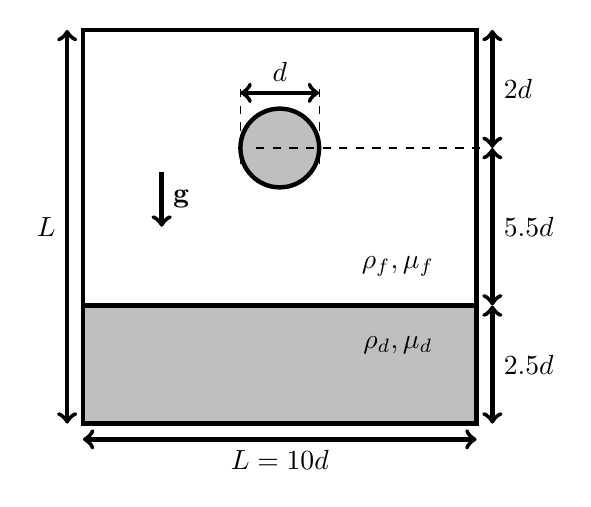
\begin{tikzpicture}[ultra thick]
        \draw (0,0) rectangle (5,5);
        \draw[fill=gray!50] (0,0) rectangle (5,1.5);
        \draw[fill=gray!50] (2.5,3.5) circle (0.5);
        \draw[<->](0,-0.2) --++ (5,0)node[midway,below]{$L  = 10 d$};
        \draw[<->](-0.2,0) --++ (0,5)node[midway,left]{$L$};
        \draw[<->](5.2,0) --++ (0,1.5)node[midway,right]{$2.5 d$};
        \draw[<->](5.2,1.5) --++ (0,2)node[midway,right]{$5.5 d$};
        \draw[<->](5.2,3.5) --++ (0,1.5)node[midway,right]{$ 2d$};
        \draw[dashed,thin](2.2,3.5) --++ (2.9,0);
        \draw[dashed,thin](2.2,3.5) --++ (2.9,0);
        \draw[->](1,3.2) --++ (0,-0.7)node[midway,right]{$\textbf{g}$};
        \draw[<->](2,4.2) --++ (1,0)node[midway,above]{$d$};
        \draw[thin,dashed](2,3.3) --++ (0,1);
        \draw[thin,dashed](3,3.3) --++ (0,1);
        \node (a) at (4,2){$\rho_f, \mu_f$};
        \node (a) at (4,1){$\rho_d, \mu_d$};
    \end{tikzpicture}
    \includegraphics[height = 0.4\textwidth]{image/VALIDATION2.0/Longmire/IMG/image-079.png}
    \caption{(left) Sketch of the computational set up at the initial time. 
    (right) Snapshot of the computational domain after the collision, with the pool interface represented in gray.
    The background color represents the velocity field magnitude, which is undisturbed, indicating a large enough domain. }
    \label{fig:schemeLong}
\end{figure}
\begin{figure}[h!]
    \centering
    \includegraphics[height = 0.3\textwidth]{image/VALIDATION2.0/Longmire/Re.pdf}
    \includegraphics[height = 0.3\textwidth]{image/VALIDATION2.0/Longmire/Dist.pdf}
    \caption{(left) Time evolution of the Reynolds number based on the droplet velocity, $Re(t) = \rho_fU d /\mu_f$ as a function of the dimensionless time, (+) numerical results of  \citet{balcazar2015multiple} (right)  position of the interfaces, ($\bullet$) top droplet surface, ($+$) bottom droplet surface, (x) pool surface. (Symbols) Experimental results of \citet{mohamed2003drop} (solid line) present numerical simulations with $d/\Delta = 20$. }
    \label{fig:resultslong}
\end{figure}
\ref{fig:resultslong} represents the comparison between our results and the experiment of \citet{mohamed2003drop} (right) and the numerical simulation of \citet{balcazar2015multiple} (left). 
The time-dependent Reynolds number as well as the interfaces positions are shown to closely match both the numerical and experiential results. 
From the very good agreement we conclude that the kinematics are well-represented even during contact for a mesh resolution of $d/\Delta = 20$.

\subsection{Mesh independence and statistical convergence for random arrays of drops}

Even though the aforementioned studies carried validations of the \texttt{Basilisk} code for rising droplets or bubbles, almost all of them considered isolated droplets or bubbles as the only validation case. 
To the author's knowledge, to this date no published study has presented a mesh independence study for random arrays of droplets or bubbles of this scale. 
As particle interactions and higher \textit{Galileo} numbers may be more challenging to model, it is primordial to investigate the mesh independence of the DNS that are carried in this work. 
In this objective we performed a DNS of a random array of $N_b=125$ droplets, with the following parameters
\begin{align*}
    \lambda = 10,
    && \zeta = 1.11,
    && Bo = 0.2,
    && Ga = 100,
    && \phi = 0.1,
    && N_b =125,
\end{align*}
with mesh resolutions of $d/\Delta = 5,\; 10,\; 18,\; 37$. 
This set of parameters have been selected following these arguments :
A viscosity ratio $\lambda = 10$ induces more vorticity at the droplets interfaces in contrast with the $\lambda = 1$ cases. 
For high inertia regimes ($Ga = 100$) the boundary layers at the droplet interfaces require the fine grid to be resolved compared to the low inertia cases. 
At $\phi = 0.1$, numerous interactions of droplets are present, implying that the good modeling of the liquid films between interfaces becomes predominant on the overall hydrodynamic, this also requires a good mesh resolution. 
% Additionally, the lower \textit{Bond} number employed here ($Bo=0.2$ instead of $Bo =0.5$) requires a higher mesh quality as well. 
For these reasons, we suppose that this case might require the finest grid among all other cases presented in this study. 
Based on this remark we can assume that if this case is mesh independent, then all cases from \ref{tab:simulations} are equally validated. 

Let us first verify the independence of the drift velocity on the mesh resolution. 
\begin{figure}[h!]
    \centering
    \includegraphics[height = 0.3\textwidth]{image/HOMOGENEOUS_NEW/VAL/tr.pdf}
    \includegraphics[height = 0.3\textwidth]{image/HOMOGENEOUS_NEW/VAL/Re.pdf}
    \caption{
        (left) Running average of the trace of $\textbf{R}$ as a function of the dimensionless time $t \sqrt{d/g}$. 
        (right) Running average of the Reynolds number based on the instantaneous volume-averaged relative velocity, $Re(t) = \rho_f U d /\mu_f$, with $U(t) = |\textbf{u}_d - \textbf{u}_c|$ for $\phi = 0.1$, $Ga=100$ and $\lambda =10$. 
        $\textbf{u}_d$ and $\textbf{u}_c$ represent the volume-averaged velocities of the dispersed phase and the continuous phase, respectively, at the dimensionless time $t \sqrt{d/g}$.
        %$\textbf{u}_p$ and $\textbf{u}_f$ are the particle and fluid phase volume averaged velocity at time $t$.
        In the legend we display the value of the mesh resolution. 
    }
    \label{fig:Re}
\end{figure}
In \ref{fig:Re} we display the running-averaged drift velocity as a function of time, for four mesh resolutions. 
The results are not as independent of the mesh resolution as the ordered array validation presented above. 
Indeed, we observe a difference of the rising Reynolds number of about $5\%$ between the $d/\Delta = 18$ and $d/\Delta = 37$ cases which is notable.
We recall that this $5\%$ error will eventually be lower for all other cases. 
The good agreement between the case  $d/\Delta = 10$ and $d/\Delta = 18$ is partially fortuitous.


% In \ref{fig:Re} (right) we display the running-averaged drift velocity as a function of time, for five mesh resolutions. 
% The results are not as independent of the mesh resolution as the ordered array validation presented above. 
% Indeed, we observe a difference of the rising Reynolds number of about $ 3\%$ between the $d/\Delta = 25$ and $d/\Delta = 60$ cases which is notable.
% We recall that this $3\%$ error will eventually be lower for all other cases. 

Now, let us turn our attention to \ref{fig:Re} (left), where we display the running average of $\text tr(\textbf{R})/r_m^2$ for different mesh resolutions.  
This figure validates two important points. 
First, we notice that the average of $\text tr(\textbf{R})/r_m^2$ appears well-converged at large $t\sqrt{d/g}$. 
This indicates that we have gathered a sufficient number of statistics to obtain accurate results. 
Secondly, it is found that the four cases converge approximately to the same value at large  $t\sqrt{d/g}$, implying that this quantity is also mesh-independent. 

\subsection{ Domain size independence study}

As discussed in the main text, the length scale of the distance between the particle layers is of the same order as the domain size. 
This raises an important question: Is the observed microstructure a physical phenomenon, or merely an artifact of the domain's size?
To address this, we conducted a DNS of a random array of $N_b=800$ droplets with a domain size of $\mathcal{L}/d = 20$. With the following dimensionless parameters:
\begin{align*}
    \lambda = 1,
    && \zeta = 1.11,
    && Bo = 0.5,
    && Ga = 80,
    && \phi = 0.05. 
\end{align*}
Note that the \textit{Galileo} number and the \textit{Bond} number are slightly different than in the original set of DNS due to numerical constraints.
We expect that these changes are not significant, so that the comparison remains valuable.


In \ref{fig:Pnst_large_domain} we compare the distribution $P_\text{nst}$ from the current case with $N_b =800$ droplets to the dataset used in this study with $N_b = 125$ droplets.
A good agreement is observed between the two distributions, although slight differences are noticeable.
These differences could be due to the different \textit{Galileo} numbers used in the larger simulation.
Nevertheless, the anisotropic behavior of $P_\text{nst}$ appears to be preserved between these two DNS.   
\begin{figure}[h!]
    \centering
    \includegraphics[height=0.205\textwidth]{image/HOMOGENEOUS_NEW/Dist/Pnst_l_1_Ga_100_PHI_0_05.pdf}
    \includegraphics[height=0.205\textwidth]{image/HOMOGENEOUS_final/Dist/Pnst_l_1_Ga_80_PHI_0_05.pdf}
    \caption{Histogram of the normalized function $P_\text{nst}$ at high inertia $Ga = 100$.
    The color map represents the values of the nearest pair distribution function. %of $P_\text{nst}$.
    The origin corresponds to the position of the \textit{\textit{test particle}}.
    The dimensionless radial and azimuthal coordinates, $|\textbf{r}|/d$ and $\theta$, correspond to the nearest neighbor position.
    The vertical direction corresponds to the flow direction, which is also the axis of symmetry for $P_\text{nst}$.
    (left) Original DNS with $N_b =125$ droplets.
    (right) Reference DNS with $N_b = 800$ droplets.}
    \label{fig:Pnst_large_domain}
\end{figure}
To provide a qualitative visualization of the system behavior, we displayed in \ref{fig:images_deux} a snapshot from both DNS. 
\begin{figure}[h!]
    \centering
    \includegraphics[width=0.45\textwidth]{image/HOMOGENEOUS_NEW/P_PHI_5_l_10_Ga_100.png}
    \includegraphics[width=0.45\textwidth]{image/HOMOGENEOUS_final/Ga_80_phi_005_l_1.png}
 %    \includegraphics[width=0.45\textwidth]{image/HOMOGENEOUS_NEW/Ga_100_phi_005_l_10.png}
    \caption{Snapshot of a simulation at $t^* = 150$ for $\phi=0.05$.
    Color map : values of the vertical component of the velocity, field on the vertical plane defined by the equation $z=0$. 
    (left)  Tipical DNS used in this study  with $\lambda = 1$ and $N_b = 125$ droplets.
    (right) A larger DNS with same $\phi$ and  $\lambda$ but with $N_b = 800$ droplets.
    }
    \label{fig:images_deux}
\end{figure}
We can observe that the DNS with $N_b = 800$ droplets also exhibits layers and clusters of droplets, similar to the original simulation. 
At this stage, we have not delved into quantitative analysis to verify if the distance between layers is consistent across both sets of simulations. 

Overall, we conclude that the domain size used in this work, $\mathcal{L}/d = 10$, is sufficient. 
Indeed, The distribution $P_\text{nst}$ remains similar in the larger domain (with $\mathcal{L}/d = 20$), and the microstructure displays the same types of particle layers and clusters.

The \texttt{Basilisk} code has been validated numerous time in previous numerical studies. 
Especially, we can cite the recent studies of \citet{innocenti2020direct} and \citet{hidman2023assessing} which both performed DNS of rising suspension of bubbles. 
Nevertheless, in this work we investigate specific statistical distribution,
and we make use of a multi-VoF method to avoid droplets coalescence, therefore a meticulous validation of the DNS is in order. 
We start by presenting a brief comparison with the reference DNS \citet{esmaeeli1999direct}. 
Afterward we present a study focusing on the interfaces' kinematic, we compare our DNS with the experimental results of \citet{mohamed2003drop} in the objective to show that the Multi-VoF method indeed capture the physics of two colliding interfaces without solving the flows in the film. 
Once the mesh and the physics are validated, a study on the convergence of the statistics is presented. 

\subsection*{Ordered array of buoyant bubbles}

From our knowledge, no simulations nor experimental results have been carried out for rising buoyant viscous drop. 
Therefore, instead we reproduced the ordered array simulation of \citet{esmaeeli1999direct} with \texttt{Basilisk} to validate the mesh definition of our DNS.  
It consists in a 3-D buoyant ordered rising array of bubbles. 
In our notation the flow parameters of the simulation reads, 
\begin{align*}
    \lambda = 10,
    && \zeta = 10,
    && Bo = 1.8,
    && Ga = 28.37,
    && \phi = 0.125.
\end{align*}
\begin{figure}[h!]
    \centering
    \includegraphics[height = 0.3\textwidth]{image/VALIDATION2.0/Loisy/Re.pdf}
    \caption{Time evolution of the Reynolds number based on the instantaneous volume averaged drift velocity, $Re(t) = \rho_fU d /\mu_f$, with $U(t) = |\textbf{u}_p - \textbf{u}_f|$ with $\phi = 0.1256$, $\zeta =\mu_r =10$ and $Ga = 29.9$.
    $\textbf{u}_p$ and $\textbf{u}_f$ are the particle and fluid phase volume averaged velocity at time $t$.}
    \label{fig:ordered_array}
\end{figure}
\ref{fig:ordered_array} display our numerical simulation against the original result of \citet{esmaeeli1999direct}.
We observe very good agreements between both studies for all mesh definition.
Additionally, we displayed the results of \citet{innocenti2020direct} for $d/\Delta = 20$ to point out a divergence with our results at the same mesh definition.  
Both our simulations and the one of \citet{innocenti2020direct} have been carried out with the  \texttt{Basilisk} code. 
The cause of this difference is in fact due to a different method of interpolation used for the viscosity coefficient $\mu$. 
We used an arithmetic mean, whereas \citet{innocenti2020direct} used a 
harmonic mean.
As a matter of fact in this regime the arithmetic mean, which will be used in this work, permit us to reach a faster convergence. 
Overall these results indicate that the criterion $d/\Delta = 30$ seems sufficient, which is consistent with the aforementioned studies.


\subsection*{Drop impact on a liquid-liquid interface}

In section, we investigate in more detail the physics behind the Multi-VoF method. 
We need to verify if we accurately capture the physics of the droplets interfaces despite the fact that we do not model accurately  the film between two droplets. 
Following \citet{balcazar2015multiple} we reproduced the experiment of drop impact on a liquid–liquid interface carried by \citet{mohamed2003drop} but with the \texttt{Basilisk} code. 
This experiment consist in letting a drop fall into a pool of the same fluid as the drop, all along the experiment the interfaces of the droplets and the pool are tracked. 
In our notation the dimensionless parameters of latter study reads, 
\begin{align*}
    Ga = 71.02 
    && Bo = 6.40
    && \lambda = 0.33
    && \zeta = 1.189
\end{align*}
Following \citet{mohamed2003drop} we defined the dimensionless time $t / t_i = t U_i(t) /d$ where $U_i(t)$ is droplet velocity at $t<0$ and where $t=0$ is the time of impact. 
Regarding the geometry of the problem we sketched in \ref{fig:schemeLong} a scheme of the initial position of the droplet in the computational domain.
Additionally, we displayed on \ref{fig:schemeLong} a snapshot of the numerical domain were we see the drop colliding the pool's interface.
Both, the drop and the pool does not merge since we use the Multi-VoF method, note that in the experiment the drop does not merge with the pool either.
This enables us to represent with DNS a physical situation where the interfaces do not coalesce, but where we use a grid definition of $d/\Delta = 30$ which is of course not sufficient to model the flow inside the film. 
\begin{figure}[h!]
    \centering
    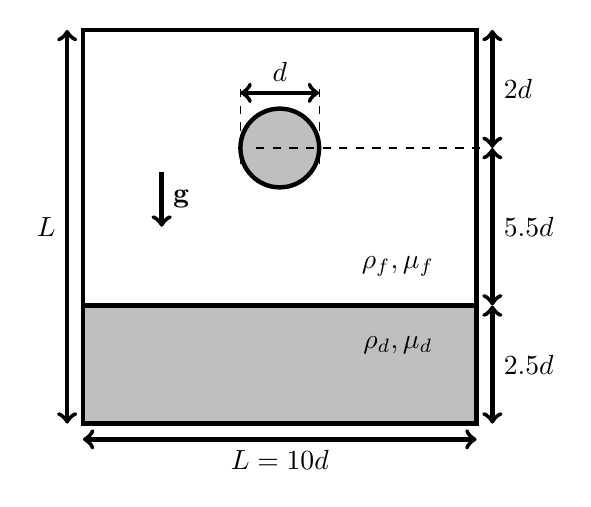
\begin{tikzpicture}[ultra thick]
        \draw (0,0) rectangle (5,5);
        \draw[fill=gray!50] (0,0) rectangle (5,1.5);
        \draw[fill=gray!50] (2.5,3.5) circle (0.5);
        \draw[<->](0,-0.2) --++ (5,0)node[midway,below]{$L  = 10 d$};
        \draw[<->](-0.2,0) --++ (0,5)node[midway,left]{$L$};
        \draw[<->](5.2,0) --++ (0,1.5)node[midway,right]{$2.5 d$};
        \draw[<->](5.2,1.5) --++ (0,2)node[midway,right]{$5.5 d$};
        \draw[<->](5.2,3.5) --++ (0,1.5)node[midway,right]{$ 2d$};
        \draw[dashed,thin](2.2,3.5) --++ (2.9,0);
        \draw[dashed,thin](2.2,3.5) --++ (2.9,0);
        \draw[->](1,3.2) --++ (0,-0.7)node[midway,right]{$\textbf{g}$};
        \draw[<->](2,4.2) --++ (1,0)node[midway,above]{$d$};
        \draw[thin,dashed](2,3.3) --++ (0,1);
        \draw[thin,dashed](3,3.3) --++ (0,1);
        \node (a) at (4,2){$\rho_f, \mu_f$};
        \node (a) at (4,1){$\rho_d, \mu_d$};
    \end{tikzpicture}
    \includegraphics[height = 0.4\textwidth]{image/VALIDATION2.0/Longmire/IMG/image-079.png}
    \caption{(left) Scheme of the computational set up at the initial time. 
    (right) Snapshot of the computational domain after the collision time, with the pool interfaces represented in gray.
    The background color represents the velocity field magnitude, which is undisturbed, indicating a large enough domain. }
    \label{fig:schemeLong}
\end{figure}
\begin{figure}[h!]
    \centering
    \includegraphics[height = 0.3\textwidth]{image/VALIDATION2.0/Longmire/Re.pdf}
    \includegraphics[height = 0.3\textwidth]{image/VALIDATION2.0/Longmire/Dist.pdf}
    \caption{(left) Time evolution of the Reynolds number based on the droplet velocity, $Re(t) = \rho_fU d /\mu_f$ in terms of the dimensionless time, (+) numerical results of  \citet{balcazar2015multiple} (right)  position of the interfaces, ($\bullet$) top droplets surface, ($+$) bot droplet surface, (x) pool surface. (Symbols) experimental result of \citet{mohamed2003drop} (solid line) present numerical simulations with $d/\Delta = 30$. }
    \label{fig:resultslong}
\end{figure}
\ref{fig:resultslong} represent the comparison between our results against the experiment of \citet{mohamed2003drop} (right) and the numerical simulation of \citet{balcazar2015multiple} (left). 
The time dependent Reynolds number as well as the interfaces positions are shown to match exactly both, the numerical and experiential results of \citet{balcazar2015multiple} and \citet{mohamed2003drop}, respectively. 
From the very good agreement obtained with the numerical and experimental results we conclude that the kinematic is preserved during the contact time for a mesh definition of $d/\Delta = 30$. 

\subsection*{Mesh independence and statistical convergence for random array of drops}

Even through aforementioned studies carried validation of the \texttt{Basilisk} code for rising droplets or bubbles, almost all of them considered isolated droplets or bubbles as the only validation case. 
As far as the author's knowledge, to this date no published study presented a mesh independence study for random array of droplets nor bubbles of this scale. 
Nevertheless, as particles interaction and higher \textit{Galileo} numbers may be more challenging to model, it is primordial to investigate the mesh independence of the exact same DNS that are carried in this work. 
In this objective we performed DNS of random array of $N_b=125$ droplets, with the following parameters,
\begin{align*}
    \lambda = 10,
    && \zeta = 1.11,
    && Bo = 1,
    && Ga = 100,
    && \phi = 0.1,
    && N_b =125,
\end{align*}
and the mesh definition is, $d/\Delta = 7.37, 14.74, 29.9 58.97$. 
We expect that the most challenging DNS simulated in this work is for the case, $\lambda = 10$ and $Ga = 100$, since it is in this range of parameters that we induce the most vorticity, which ultimately require good mesh definition. 
Additionally, in opposition to the ordered array case, this case includes droplets interaction, which ultimately induce more numerical complexities to tackles. 
Based on this remark we can assume that if this case is mesh independent, then all cases from \ref{tab:simulations} must be since this is the most challenging scenario.   

Let's first verify the independence of the drift velocity on the mesh definition. 
\begin{figure}[h!]
    \centering
    \includegraphics[height = 0.3\textwidth]{image/HOMOGENEOUS_NEW/VAL/Re.pdf}
    \caption{
        Running average of the Reynolds number based on the instantaneous volume averaged drift velocity, $Re(t) = \rho_fU d /\mu_f$, with $U(t) = |\textbf{u}_p - \textbf{u}_f|$ for $\phi = 0.1$, $Ga=100$ and $\lambda =10$.
        $\textbf{u}_p$ and $\textbf{u}_f$ are the particle and fluid phase volume averaged velocity at time $t$.
        In the legend we display the value of the mesh definition. 
    }
    \label{fig:Re}
\end{figure}
In \ref{fig:Re} we display the running averaged drift velocity in terms of time, for four mesh definition. 
The results are not as independent of the mesh definition as the order array validation presented above. 
Indeed, we observe a difference of the rising Reynolds number of about $5\%$ between the $d/\Delta = 29.49$ and $d/\Delta = 58.97$ cases which is notable.
We recall that this $5\%$ error will eventually be lower for all other cases. 
The good agreement between the case  $d/\Delta = 14.74$ and $d/\Delta = 29.49$ is partially fortuitous.

Now let's study the mesh influence on the statistics. 
It is clear from \ref{fig:apstat} (left) that both mesh definition produce nearly the same radial distribution, no notable difference is identified. 
In \ref{fig:apstat} (middle) we can observe the age distribution for both mesh definition. 
It is clear that refining the mesh induce a difference in the age distribution. 
As, a matter of fact it has a small impact on the mean age, $\tau_p = 6.96$ for the lower definition, and $\tau_p = 6.14$ for the finest grid.
This makes a $10\%$ error, but as mentioned above this is probably the highest error that we could encounter among all cases. 
\begin{figure}
    \centering
    \includegraphics[height = 0.24\textwidth]{image/HOMOGENEOUS_NEW/VAL/Pr.pdf}
    \includegraphics[height = 0.24\textwidth]{image/HOMOGENEOUS_NEW/VAL/Pa.pdf}
    \includegraphics[height = 0.24\textwidth]{image/HOMOGENEOUS_NEW/VAL/w.pdf}
    \caption{
        Statistical averaged functions for two mesh definition. 
        (left) Radial normalized probability density function  $P_r(\textbf{x},|\textbf{r}|,t)/P_\text{th}$, in terms of the dimensionless radial position. 
        (middle) Probability density function of the age distribution $P_a(\textbf{x},t,a)$. 
        (right) Nearest averaged dimensionless approach velocity for both mesh definition, in terms of the dimensionless age. 
    }
    \label{fig:apstat}
\end{figure}
Even through an error is identified on the mean age of interaction we still notice that both nearest averaged dimensionless approach velocity on \ref{fig:apstat} (right) match perfectly. 
\begin{figure}[h!]
    \centering
    \includegraphics[height = 0.3\textwidth]{image/HOMOGENEOUS_NEW/VAL/U_rel_ndc_25.pdf}
    \includegraphics[height = 0.3\textwidth]{image/HOMOGENEOUS_NEW/VAL/U_rel_ndc_35.pdf}
    \caption{Quiver plots of the relative averaged velocity field $\textbf{w}^\text{r}(\textbf{x},\textbf{r},t)$ colored by the averaged dimensionless age $a^r(\textbf{x},\textbf{r},t)$, for $\phi = 0.05$ and $Ga = 100$. 
    (left) Low mesh definition.
    (right) High mesh definition. 
    }
    \label{fig:velap}
\end{figure}
Regarding, the 2D fields  $\textbf{w}^\text{r}(\textbf{x},\textbf{r},t)$ we can see that no notable difference can be identified, if it is not the slight difference in the value of the age scale. 


Overall, the one dimensional and two-dimensional conditioned statistics are almost independent of the mesh definition. 
By obtaining the same statistics with two independent DNS makes us confident on the fact that our numerical samples is large enough.
Indeed, if the samples were not sufficient we would have obtained two different distribution functions, thus we can be sure that the statistics have well converged. 
The slight difference in rising velocity and age distribution found for these Reynolds number must be acknowledged.
As mentioned at the beginning, this case is in fact very challenging as the volume fraction of droplets is consequent which induce numerous inertial interactions. 
Nevertheless, we can be sure that our final results is accurate at most with a $5\%$ error for this case, and probably less for the others cases. 
These, error testify for the very challenging  aspect of these simulations. 
Overall, we have great confidence in the statistical and physical representativity of our DNS results. 
\section{Age distribution at low \textit{Galileo} numbers}
\label{ap:age}

We provide additional age distribution for low \textit{Galileo} number to support the argumentation in the body of the text. 
\begin{figure}[h!]
    \centering
    \includegraphics[height = 0.3\textwidth]{image/HOMOGENEOUS_NEW/Dist/Pa_l_1_Ga_10.pdf}
    \includegraphics[height = 0.3\textwidth]{image/HOMOGENEOUS_NEW/Dist/Pa_l_10_Ga_10.pdf}
    \caption{(left) Age distribution at $\lambda = 10$ and $Ga = 10$ for : (solid line) $\phi = 0.2$; (dash dotted line) $\phi = 0.1$; (dashed line) $\phi =0.05$; (dotted line) $\phi = 0.01$. 
    (right) Mean dimensionless age in terms of the volume fraction $\phi$ for : 
    ($\bullet$) $Ga=1$; ($\blacktriangle$) $ Ga = 10$; ($\blacksquare$) $Ga = 50$ ($\blacklozenge$) $Ga =100$.
    The age and $\tau_a$ are made dimensionless with $U/d$ where $U$ is the drift-velocity between the dispersed and continuous phase.  }
    \label{fig:age_picture}
\end{figure}


\addcontentsline{toc}{chapter}{Bibliography}
\bibliography{Bib/bib_bulles.bib}


\end{document}
